\section{Results} \label{appendix:results}

\noindent In this appendix we first explain our method for selecting the background variables that we control for when estimating treatment effects.\footnote{This is a separate discussion from the election of variables to forecast life-cycle profiles of labor income and other outcomes. For that discussion see Appendix~\ref{appendix:methodology}.} Then, we present the treatment effects of the center-based treatment in ABC/CARE estimates for the 95 main outcomes we consider. For each set of estimates, we first present a summary of the effect of the program using a combining function counting the number of socially positive treatment effects. We then present tables of treatment effect estimates for each outcome. Finally, we present the treatment effect estimates using the step-down procedure to test multiple hypotheses.\\

\subsection{Background Variables} \label{appendix:bvariables}

\noindent We select three out of fourteen potential variables that best predict the relevant outcomes of interest, i.e. the outcomes we test treatment effects for. We list the fourteen variables in Table~\ref{tab:pselectvars} and bold the three we choose.

\singlespacing
\begin{table}[H]
\centering
\begin{threeparttable}
\caption{Background Variables}
\label{tab:pselectvars}
\begin{tabular}{C{5cm} C{5cm} C{5cm}}
\toprule
\textbf{Maternal IQ}			& \textbf{Maternal education}		& Mother's age at birth \\
High Risk Index		& Parent income			& Premature birth \\
1 minute Apgar score	& 5 minute Apgar score	& Mother married \\
Teen pregnancy		& \textbf{Father at home}			& Number of siblings \\
Cohort 				& Mother is employed		& \\
\bottomrule
\end{tabular}
\begin{tablenotes}
\footnotesize
\item Note: This table lists the variables we permute over when selecting the background variables we control for in our estimations. We bold the variables we choose based on the procedure explained in this section.
\end{tablenotes}
\end{threeparttable}
\end{table} 
\doublespacing

\noindent We briefly formalize the choice of the control sets based on most predictive models in the next lines.\\ 

\noindent Let $\mathcal{M}$ be the set of all the models we consider. In our application, $\mathcal{M}$ consists of all linear regressions of an outcome of interest on the different combinations of background variables. $m \in \mathcal{M}$ is one of such models. We choose the model minimizing the Bayesian Information Criterion (BIC) by ranking them according to their likelihood. That is, according to their posterior probability given the data. The data, in this case, are the dependent variable being predicted together with the background variables in each combination. We denote this by $\Pr( m | \text{Data} )$.\\

\noindent Using Bayes Rule and the law of total probability, 

\begin{eqnarray}
\Pr( m | \text{Data} ) &=& \frac{\Pr(\text{Data} | m)\times \Pr(m)}{ \Pr(\text{Data})}\\ \nonumber
&=& \frac{\Pr(\text{Data} | m)\times \Pr(m)}{\sum \limits _{m' \in M} \Pr (\text{Data} | m') \Pr(m')} \\ \nonumber
&\propto& \Pr (\text{Data} | m) \times \Pr(m),
\end{eqnarray}

\noindent where $\Pr(m)$ is the prior probability of model $m$ and $\Pr(\text{Data} | m)$ is the probability of observing $\text{Data}$ under model $m$.\\

\noindent There are various approaches to rank the the likelihood of each model. Examples include rankings based on Bayesian Information Criterion (Schwarz), the Hannan-Quinn Information Criterion (HWIC), and the Akaike Information Criterion (AIC). We use the first approach because it has appealing consistency properties \citep{Diebold_2007_Forecasting}. This criterion minimizes the following loss function: $2 \log [\Pr( \text{Data} | m)]$. We follow an specific approximation developed by \citet{Claeskens-Hjort_2008_Model-Selection}, which assumes uniform priors and simplifies the computation of the loss function.\\

\noindent This procedure allows us to choose one control set per outcomes of interest. To gain consistency across all specifications, we sum the BIC across all outcomes and choose the background variables with lower average across models. These background variables form our control set across all estimations and appear bold in Table~\ref{tab:pselectvars}. 

\subsubsection{Sensitivity Analysis}

\noindent An immediate route of inquiry has to do with the sensitivity of our estimates to the choice of background variables. Especially in the context of our small sample, in which estimates can be volatile to different model specifications. To investigate this, we estimate treatment effects for the three counterfactuals we consider under all possible control sets of the three variables we can form with the background variables in Table~\ref{tab:pselectvars}. We also consider all possible control sets of one and two variables in Table~\ref{tab:pselectvars}. For brevity, we present this exercise for two outcomes, employment and education. Similar exercises for the 95 main outcomes we consider are available upon request.\\

\noindent Figure~\ref{fig:senstnb} to Figure~\ref{fig:senstap} display the results from this exercise. In any case, the support of the distributions is very compressed leading us to conclude that there is little sensitivity to the choice of controls sets.

\begin{sidewaysfigure}[!htbp]
\centering
\caption{Sensitiviy to Choice of Control Set, Treatment vs. Next Best}\label{fig:senstnb}
\begin{subfigure}[h]{0.4\textwidth}
		\centering
		\caption{Years of Education, Males}
		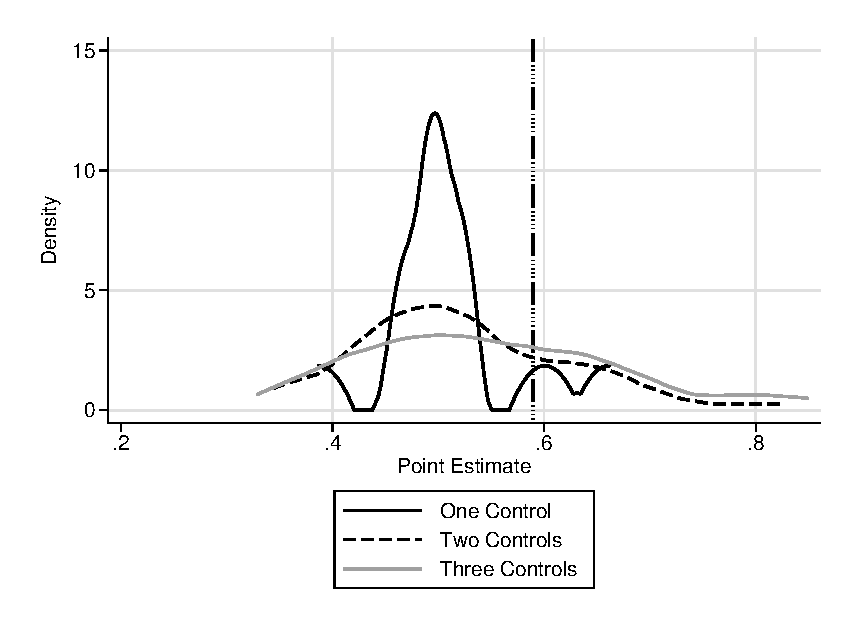
\includegraphics[width=\textwidth]{output/sencontrols_male_years_30y_itt_wctrl.eps}
\end{subfigure}%
\begin{subfigure}[h]{0.4\textwidth}
	\centering
	\caption{Employment, Males}
		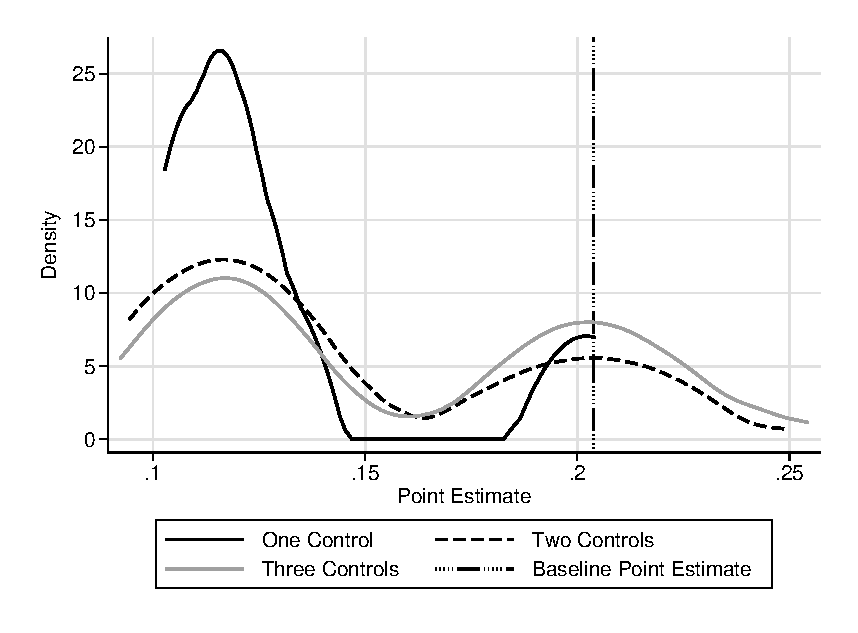
\includegraphics[width=\textwidth]{output/sencontrols_male_si30y_works_itt_wctrl.eps}
\end{subfigure}
\begin{subfigure}[h]{0.4\textwidth}
		\centering
		\caption{Years of Education, Females}
		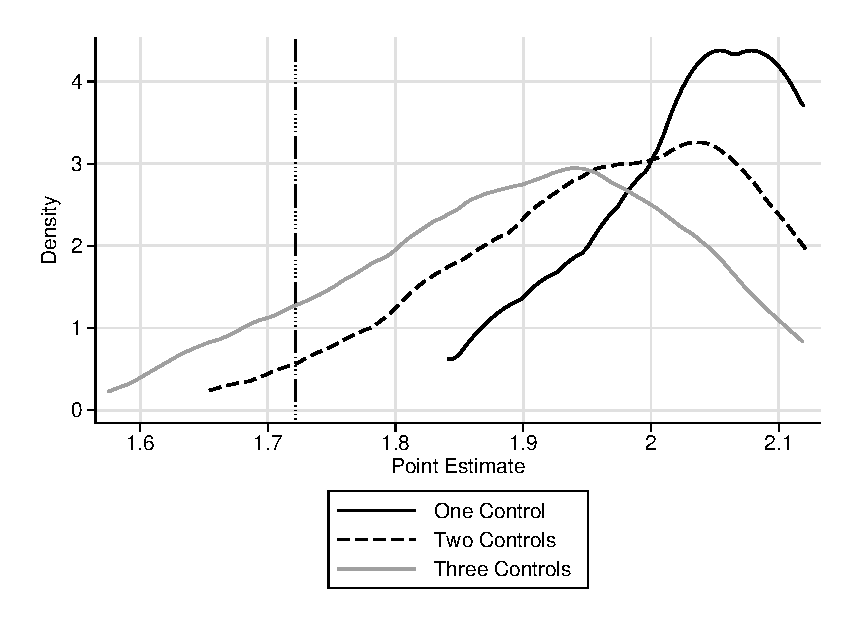
\includegraphics[width=\textwidth]{output/sencontrols_female_years_30y_itt_wctrl.eps}
\end{subfigure}%
\begin{subfigure}[h]{0.4\textwidth}
	\centering
	\caption{Employment, Females}
		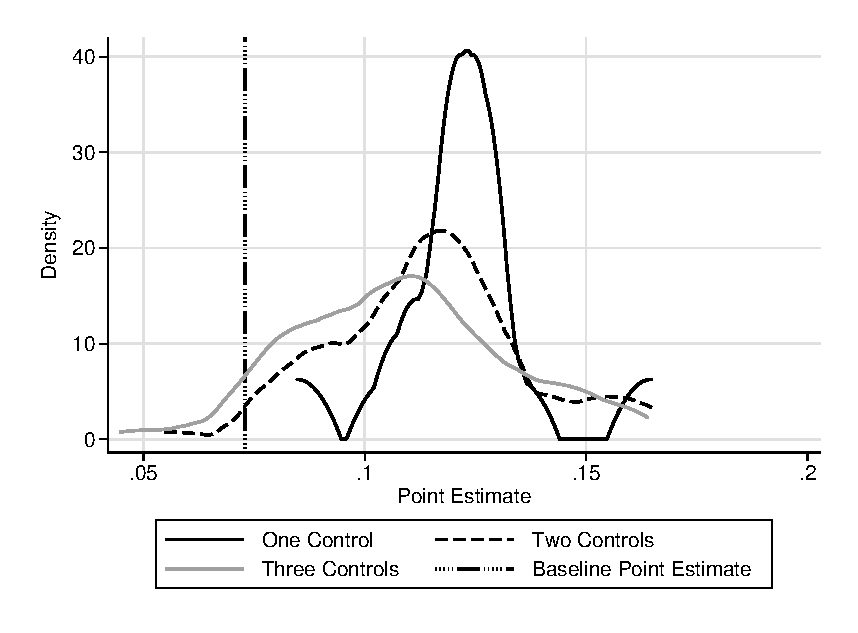
\includegraphics[width=\textwidth]{output/sencontrols_female_si30y_works_itt_wctrl.eps}
\end{subfigure}
\footnotesize \justify
Note: Panel (a) displays the distribution of the treatment effect estimate of the treatment compared to next best counterfactual for males years of education. The distribution is obtained by using all possible combinations of one, two, and three background variables listed in Table~\ref{tab:pselectvars}. The horizontal line marks the baseline estimate we use. The reminder panels present analogous distributions for the outcomes and genders indicated in the title.\\
\end{sidewaysfigure}

\begin{sidewaysfigure}[!htbp]
\centering
\caption{Sensitiviy to Choice of Control Set, Treatment vs. Stay at Home}
\begin{subfigure}[h]{0.4\textwidth}
		\centering
		\caption{Years of Education, Males}
		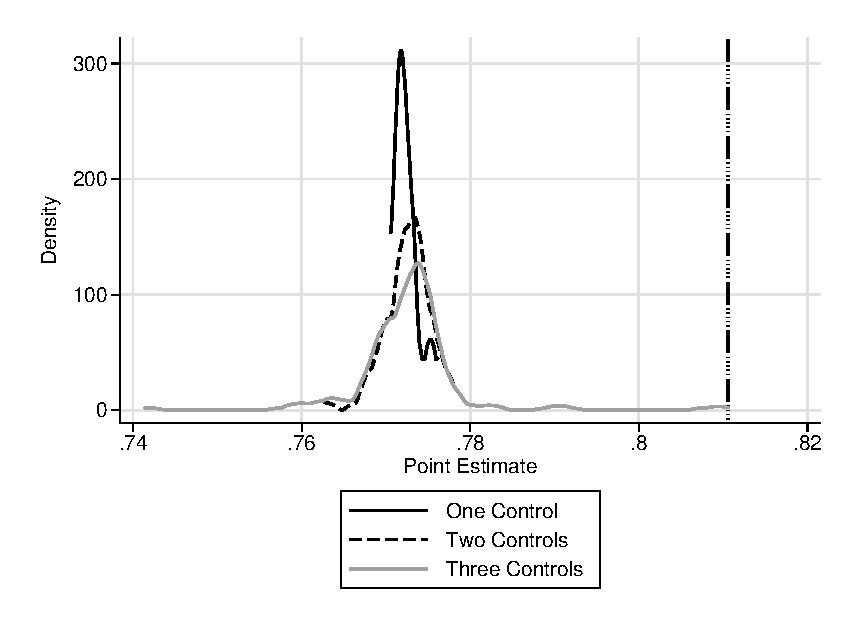
\includegraphics[width=\textwidth]{output/sencontrols_male_years_30y_epan_ipw_P0.eps}
\end{subfigure}%
\begin{subfigure}[h]{0.4\textwidth}
	\centering
	\caption{Employment, Males}
		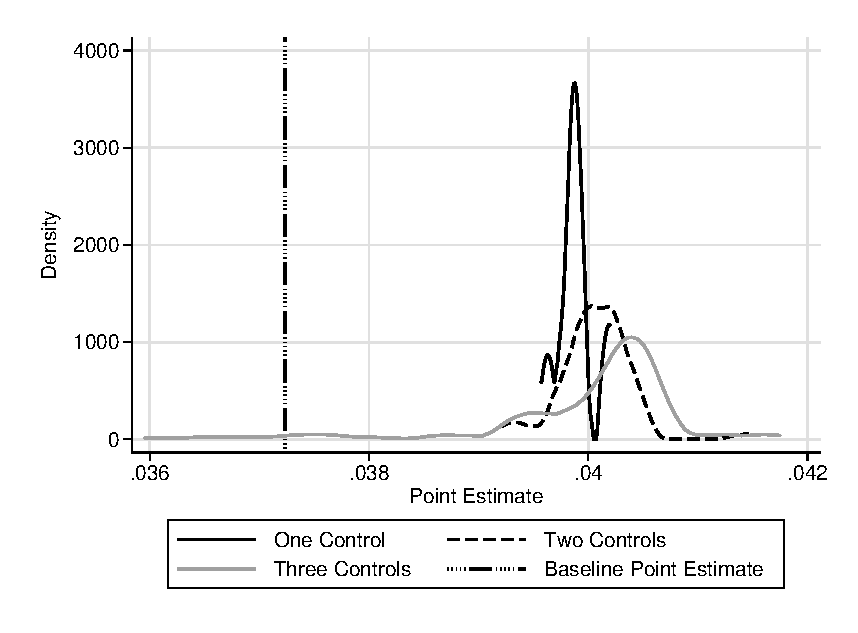
\includegraphics[width=\textwidth]{output/sencontrols_male_si30y_works_epan_ipw_P0.eps}
\end{subfigure}
\begin{subfigure}[h]{0.4\textwidth}
		\centering
		\caption{Years of Education, Females}
		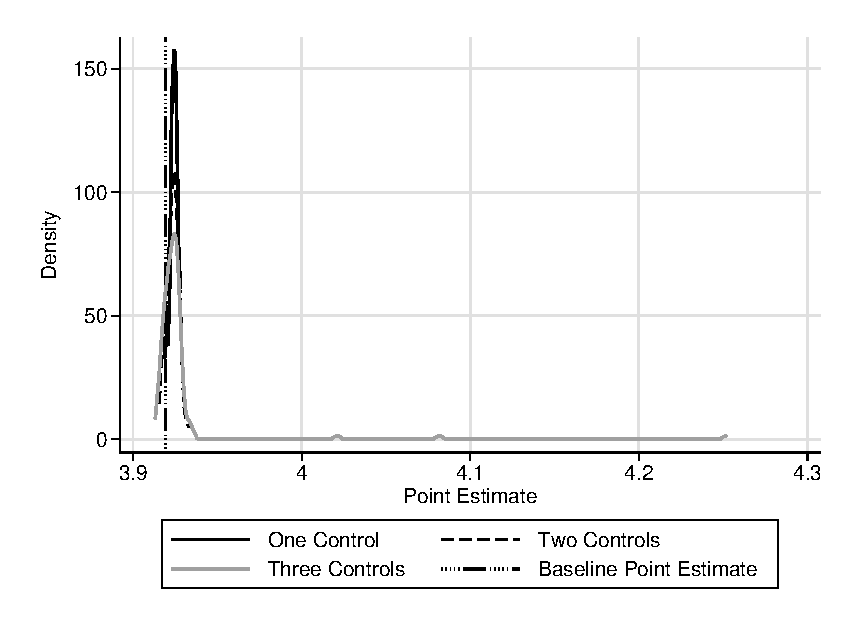
\includegraphics[width=\textwidth]{output/sencontrols_female_years_30y_epan_ipw_P0.eps}
\end{subfigure}%
\begin{subfigure}[h]{0.4\textwidth}
	\centering
	\caption{Employment, Females}
		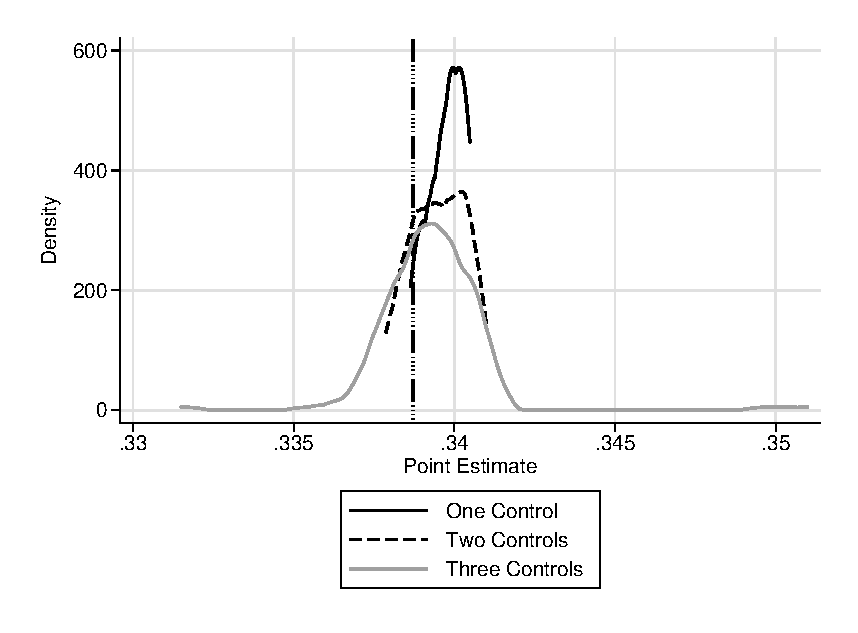
\includegraphics[width=\textwidth]{output/sencontrols_female_si30y_works_epan_ipw_P0.eps}
\end{subfigure}
\footnotesize \justify
Note: Panel (a) displays the distribution of the treatment effect estimate of the treatment compared to stay at home counterfactual for males years of education. The distribution is obtained by using all possible combinations of one, two, and three background variables listed in Table~\ref{tab:pselectvars}. The horizontal line marks the baseline estimate we use. The reminder panels present analogous distributions for the outcomes and genders indicated in the title.\\
\end{sidewaysfigure}

\begin{sidewaysfigure}[!htbp]
\centering
\caption{Sensitiviy to Choice of Control Set, Treatment vs. Alternative Preschool}\label{fig:senstap}
\begin{subfigure}[h]{0.4\textwidth}
		\centering
		\caption{Years of Education, Males}
		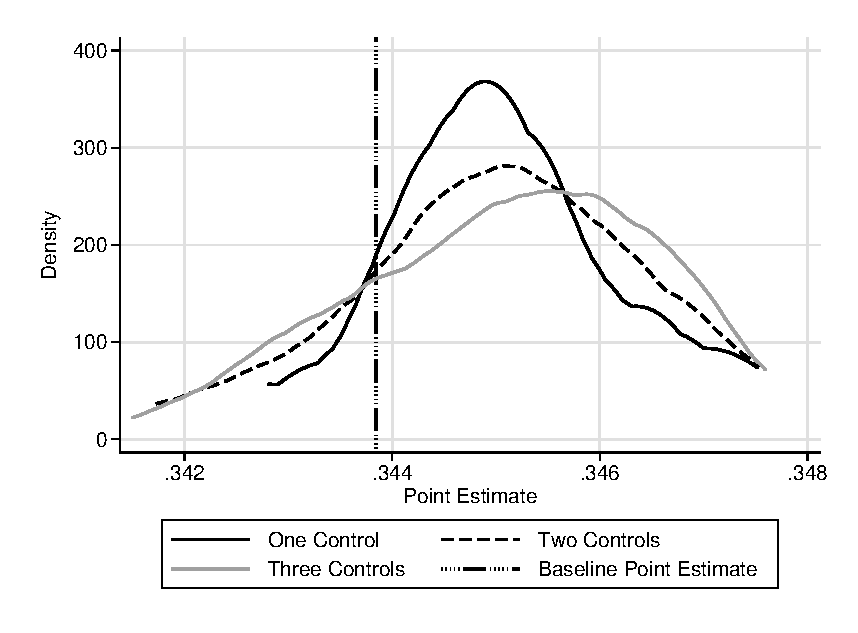
\includegraphics[width=\textwidth]{output/sencontrols_male_years_30y_epan_ipw_P1.eps}
\end{subfigure}%
\begin{subfigure}[h]{0.4\textwidth}
	\centering
	\caption{Employment, Males}
		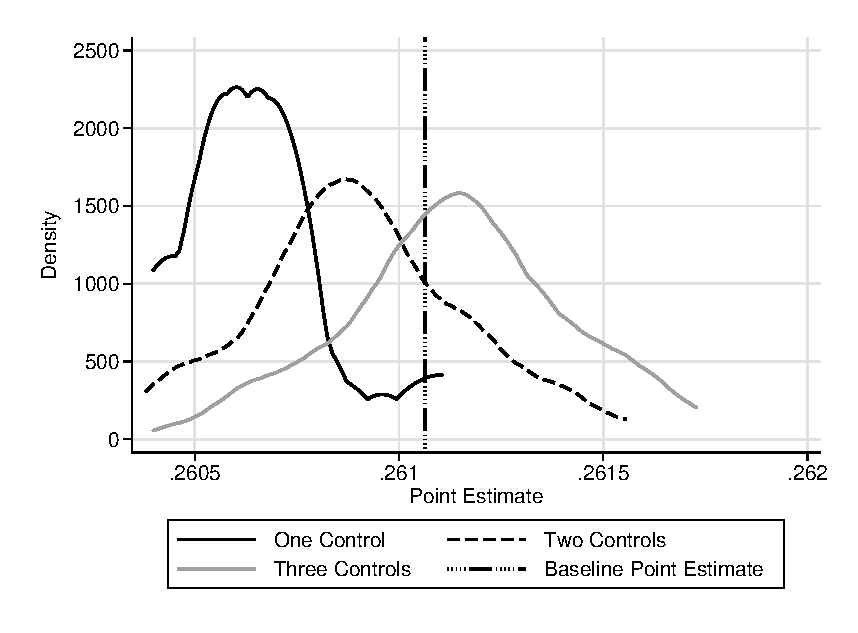
\includegraphics[width=\textwidth]{output/sencontrols_male_si30y_works_epan_ipw_P1.eps}
\end{subfigure}
\begin{subfigure}[h]{0.4\textwidth}
		\centering
		\caption{Years of Education, Females}
		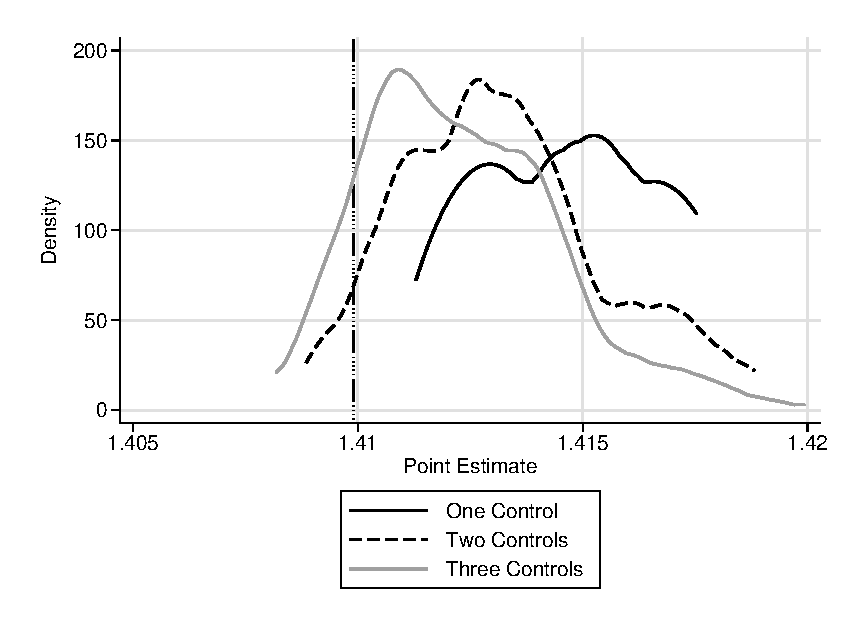
\includegraphics[width=\textwidth]{output/sencontrols_female_years_30y_epan_ipw_P1.eps}
\end{subfigure}%
\begin{subfigure}[h]{0.4\textwidth}
	\centering
	\caption{Employment, Females}
		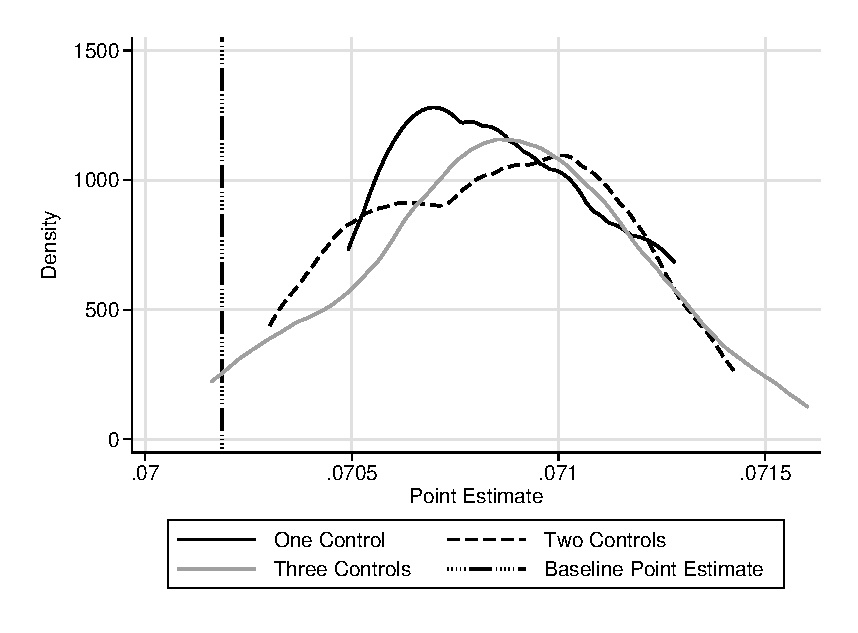
\includegraphics[width=\textwidth]{output/sencontrols_female_si30y_works_epan_ipw_P1.eps}
\end{subfigure}
\footnotesize \justify
Note: Panel (a) displays the distribution of the treatment effect estimate of the treatment compared to alternative preschool counterfactual for males years of education. The distribution is obtained by using all possible combinations of one, two, and three background variables listed in Table~\ref{tab:pselectvars}. The horizontal line marks the baseline estimate we use. The reminder panels present analogous distributions for the outcomes and genders indicated in the title.\\
\end{sidewaysfigure}

\subsection{Outcomes of Interest}

\noindent Table \ref{tab:main-outcomes} lists the 95 main outcomes that we test in our main analysis. We reverse the outcomes for which we consider a negative treatment effect socially positive. \\

\singlespacing
\begin{center}
\begin{ThreePartTable}

\begin{TableNotes}[para,flushleft]
Note: This table lists the outcomes that we test treatment effects for. We reverse the outcomes for which we consider a negative treatment effect socially positive.
\end{TableNotes}


\begin{longtable}{L{4cm} L{5cm} C{1cm} C{1cm} C{1.2cm} C{1.5cm}}

\caption{Outcome Variables} \\

\toprule
Category	&	Variable	&	Age	&	ABC	&	CARE	&	Reversed	\\ \midrule
\endfirsthead

\toprule
Category	&	Variable	&	Age	&	ABC	&	CARE	&	Reversed	\\ \midrule
\endhead

\midrule
\endfoot

%\bottomrule
\endlastfoot

IQ Scores	&	Std. IQ Test	&	2	&	\checkmark	&	\checkmark	&		\\
	&		&	2.5	&		&	\checkmark	&		\\
	&		&	3	&	\checkmark	&	\checkmark	&		\\
	&		&	3.5	&	\checkmark	&	\checkmark	&		\\
	&		&	4	&	\checkmark	&	\checkmark	&		\\
	&		&	4.5	&	\checkmark	&	\checkmark	&		\\
	&		&	5	&	\checkmark	&	\checkmark	&		\\
	&		&	6.6	&	\checkmark	&	\checkmark	&		\\
	&		&	7	&	\checkmark	&	\checkmark	&		\\
	&		&	8	&	\checkmark	&	\checkmark	&		\\
	&		&	12	&	\checkmark	&	\checkmark	&		\\
	&		&	15	&	\checkmark	&		&		\\
	&		&	21	&	\checkmark	&		&		\\
	&	IQ Factor	&	2 to 5	&	\checkmark	&	\checkmark	&		\\
	&		&	6 to 12	&	\checkmark	&	\checkmark	&		\\
	&		&	15 to 21	&	\checkmark	&		&		\\     
\\[0.1cm]
Achievement Scores	&	Std. Achv.  Test	&	5.5	&	\checkmark	&	\checkmark	&		\\
	&		&	6	&	\checkmark	&	\checkmark	&		\\
	&		&	6.5	&	\checkmark	&		&		\\
	&		&	7	&	\checkmark	&		&		\\
	&		&	7.5	&	\checkmark	&	\checkmark	&		\\
	&		&	8	&	\checkmark	&	\checkmark	&		\\
	&		&	8.5	&	\checkmark	&	\checkmark	&		\\
	&		&	12	&		&	\checkmark	&		\\
	&		&	15	&	\checkmark	&		&		\\
	&		&	21	&	\checkmark	&		&		\\
	&	PIAT Math Std. Score	&	7	&	\checkmark	&	\checkmark	&		\\
	&	Achievement Factor	&	5.5 to 12	&	\checkmark	&	\checkmark	&		\\
	&		&	15 to 21	&	\checkmark	&		&		\\
\\[0.1cm]
HOME Scores	&	HOME Score	&	0.5	&	\checkmark	&	\checkmark	&		\\
	&		&	1.5	&	\checkmark	&	\checkmark	&		\\
	&		&	2.5	&	\checkmark	&	\checkmark	&		\\
	&		&	3.5	&	\checkmark	&	\checkmark	&		\\
	&		&	4.5	&	\checkmark	&	\checkmark	&		\\
	&		&	8	&	\checkmark	&	\checkmark	&		\\
	&	HOME Factor	&	0.5 to 8	&	\checkmark	&	\checkmark	&		\\
\\[0.1cm]
Parent Income	&	Parental income	&	1.5	&	\checkmark	&	\checkmark	&		\\
	&		&	2.5	&	\checkmark	&	\checkmark	&		\\
	&		&	3.5	&	\checkmark	&	\checkmark	&		\\
	&		&	4.5	&	\checkmark	&	\checkmark	&		\\
	&		&	8	&	\checkmark	&		&		\\
	&		&	12	&	\checkmark	&		&		\\
	&		&	15	&	\checkmark	&		&		\\
	&	Parental Income Factor	&	1.5 to 15	&	\checkmark	&	\checkmark	&		\\
\\[0.1cm]
Mother's Employment	&	Mother Works	&	2	&	\checkmark	&	\checkmark	&		\\
	&		&	3	&	\checkmark	&	\checkmark	&		\\
	&		&	4	&	\checkmark	&	\checkmark	&		\\
	&		&	5	&	\checkmark	&	\checkmark	&		\\
	&		&	21	&	\checkmark	&		&		\\
	&	Mother Works Factor	&	2 to 21	&	\checkmark	&	\checkmark	&		\\
\\[0.1cm]
Mother's Education	&	Mother's Years of Edu.	&	2	&	\checkmark	&		&		\\
	&		&	3	&	\checkmark	&		&		\\
	&		&	4	&	\checkmark	&		&		\\
	&		&	5	&	\checkmark	&		&		\\
	&		&	9	&	\checkmark	&		&		\\
	&	Mother's Edu. Factor	&	2 to 9	&	\checkmark	&		&		\\
\\[0.1cm]
Father at Home	&	Father at Home	&	2	&	\checkmark	&	\checkmark	&		\\
	&		&	3	&	\checkmark	&	\checkmark	&		\\
	&		&	4	&	\checkmark	&	\checkmark	&		\\
	&		&	5	&	\checkmark	&	\checkmark	&		\\
	&		&	8	&	\checkmark	&	\checkmark	&		\\
	&	Father at Home Factor	&	2 to 8	&	\checkmark	&	\checkmark	&		\\
\\[0.1cm]
Adoption	&	Ever Adopted	&	       	&	\checkmark	&		&		\\
\\[0.1cm]
Education	&	Graduated High School	&	30	&	\checkmark	&	\checkmark	&		\\
	&	Attended Voc./Tech./Com. College	&	30	&	\checkmark	&	\checkmark	&		\\
	&	Graduated 4-year College	&	30	&	\checkmark	&	\checkmark	&		\\
	&	Years of Edu.	&	30	&	\checkmark	&	\checkmark	&		\\
	&	Education Factor	&	30	&	\checkmark	&	\checkmark	&		\\
\\[0.1cm]
Employment and Income	&	Employed	&	30	&	\checkmark	&	\checkmark	&		\\
	&	Labor Income	&	21	&	\checkmark	&	\checkmark	&		\\
	&		&	30	&	\checkmark	&	\checkmark	&		\\
	&	Public-Transfer Income	&	21	&	\checkmark	&	\checkmark	&	\checkmark	\\
	&		&	30	&	\checkmark	&	\checkmark	&	\checkmark	\\
	&	Employment Factor	&	21 to 30	&	\checkmark	&	\checkmark	&		\\
\\[0.1cm]
Crime	&	Total Felony Arrests	&	Mid-30s	&	\checkmark	&	\checkmark	&	\checkmark	\\
	&	Total Misdemeanor Arrests	&	Mid-30s	&	\checkmark	&	\checkmark	&	\checkmark	\\
	&	Total Years Incarcerated	&	30	&	\checkmark	&	\checkmark	&	\checkmark	\\
	&	Crime Factor	&	30 to Mid-30s	&	\checkmark	&	\checkmark	&	\checkmark	\\
\\[0.1cm]
Tobacco, Drugs, Alcohol	&	Cig. Smoked per day last month	&	30	&	\checkmark	&	\checkmark	&	\checkmark	\\
	&	Days drank alcohol last month	&	30	&	\checkmark	&	\checkmark	&	\checkmark	\\
	&	Days binge drank alcohol last month	&	30	&	\checkmark	&	\checkmark	&	\checkmark	\\
	&	Self-reported drug user	&	Mid-30s	&	\checkmark	&	\checkmark	&	\checkmark	\\
	&	Substance Use Factor	&	30 to Mid-30s	&	\checkmark	&	\checkmark	&	\checkmark	\\
\\[0.1cm]
Self-Reported Health	&	Self-reported Health	&	30	&	\checkmark	&	\checkmark	&	\checkmark	\\
	&		&	Mid-30s	&	\checkmark	&	\checkmark	&	\checkmark	\\
	&	Self-reported Health Factor	&	30 to Mid-30s	&	\checkmark	&	\checkmark	&	\checkmark	\\
\\[0.1cm]
Hypertension	&	Systolic Blood Pressure (mm Hg)	&	Mid-30s	&	\checkmark	&	\checkmark	&	\checkmark	\\
	&	Diastolic Blood Pressure (mm Hg)	&	Mid-30s	&	\checkmark	&	\checkmark	&	\checkmark	\\
	&	Prehypertension	&	Mid-30s	&	\checkmark	&	\checkmark	&	\checkmark	\\
	&	Hypertension	&	Mid-30s	&	\checkmark	&	\checkmark	&	\checkmark	\\
	&	Hypertension Factor	&	Mid-30s	&	\checkmark	&	\checkmark	&	\checkmark	\\
\\[0.1cm]
Cholesterol	&	High-Density Lipoprotein Chol. (mg/dL)	&	Mid-30s	&	\checkmark	&	\checkmark	&		\\
	&	Dyslipidemia	&	Mid-30s	&	\checkmark	&	\checkmark	&	\checkmark	\\
	&	Cholesterol Factor	&	Mid-30s	&	\checkmark	&	\checkmark	&	\checkmark	\\
\\[0.1cm]
Diabetes	&	Hemoglobin Level (\%)	&	Mid-30s	&	\checkmark	&	\checkmark	&	\checkmark	\\
	&	Prediabetes	&	Mid-30s	&	\checkmark	&	\checkmark	&	\checkmark	\\
	&	Diabetes	&	Mid-30s	&	\checkmark	&	\checkmark	&	\checkmark	\\
	&	Diabetes Factor	&	Mid-30s	&	\checkmark	&	\checkmark	&	\checkmark	\\
\\[0.1cm]
Vitamin D Deficiency	&	Vitamin D Deficiency	&	Mid-30s	&	\checkmark	&	\checkmark	&	\checkmark	\\
\\[0.1cm]
Obesity	&	Measured BMI	&	Mid-30s	&	\checkmark	&	\checkmark	&	\checkmark	\\
	&	Obesity	&	Mid-30s	&	\checkmark	&	\checkmark	&	\checkmark	\\
	&	Severe Obesity	&	Mid-30s	&	\checkmark	&	\checkmark	&	\checkmark	\\
	&	Waist-hip Ratio	&	Mid-30s	&	\checkmark	&	\checkmark	&	\checkmark	\\
	&	Abdominal Obesity	&	Mid-30s	&	\checkmark	&	\checkmark	&	\checkmark	\\
	&	Framingham Risk Score	&	Mid-30s	&	\checkmark	&	\checkmark	&	\checkmark	\\
	&	Obesity Factor	&	Mid-30s	&	\checkmark	&	\checkmark	&	\checkmark	\\
\\[0.1cm]
Mental Health (BSI)	&	Somatization	&	21	&	\checkmark	&	\checkmark	&	\checkmark	\\
	&		&	34	&	\checkmark	&	\checkmark	&	\checkmark	\\
	&	Depression	&	21	&	\checkmark	&	\checkmark	&	\checkmark	\\
	&		&	34	&	\checkmark	&	\checkmark	&	\checkmark	\\
	&	Anxiety	&	21	&	\checkmark	&	\checkmark	&	\checkmark	\\
	&		&	34	&	\checkmark	&	\checkmark	&	\checkmark	\\
	&	Hostility	&	21	&	\checkmark	&	\checkmark	&	\checkmark	\\
	&		&	34	&	\checkmark	&	\checkmark	&	\checkmark	\\
	&	Global Severity Index	&	21	&	\checkmark	&	\checkmark	&	\checkmark	\\
	&		&	34	&	\checkmark	&	\checkmark	&	\checkmark	\\
	&	Mental Health Factor	&	21 and 34	&	\checkmark	&	\checkmark	&	\checkmark	\\
\\[0.1cm]
Child Behavior (CAS)	&	Participates in Activity	&	12	&	\checkmark	&		&		\\
	&	Time Spent Reading	&	12	&	\checkmark	&		&		\\
	&	Good Description of Self	&	12	&	\checkmark	&		&		\\
	&	Views Self as Dumb	&	12	&	\checkmark	&		&	\checkmark	\\
	&	Views Self as Clumsy	&	12	&	\checkmark	&		&	\checkmark	\\
	&	Views Self as Not Liked	&	12	&	\checkmark	&		&	\checkmark	\\
	&	Proud About Self	&	12	&	\checkmark	&		&		\\
	&	Family Proud of You	&	12	&	\checkmark	&		&		\\
	&	Feels Inadequate, Inferior	&	12	&	\checkmark	&		&	\checkmark	\\
	&	Withdraws Excessively	&	12	&	\checkmark	&		&	\checkmark	\\
	&	Ignores Situation	&	12	&	\checkmark	&		&	\checkmark	\\
	&	Not Cope with Prob.	&	12	&	\checkmark	&		&	\checkmark	\\
	&	Often Mad of Angry	&	12	&	\checkmark	&		&	\checkmark	\\
	&	Impulsivity	&	12	&	\checkmark	&		&	\checkmark	\\
	&	Significant Fears	&	12	&	\checkmark	&		&	\checkmark	\\
	&	Denies Any Worries	&	12	&	\checkmark	&		&	\checkmark	\\

\bottomrule
	
\insertTableNotes
\end{longtable}
\end{ThreePartTable}
\end{center}




\doublespacing

\subsection{Estimates}

\noindent Table~\ref{table:abccare_rslt_pooled_counts} shows that across all methods of estimation, pooling males and females, over 70\% of the treatment effect estimates are socially positive. When conditioning on 10\% statistical significance, almost 40\% of all estimates are socially positive. These statistics allow us to reject the hypothesis that the treatment and control groups have the same marginal distributions in outcomes. \\

\noindent For both males and females, we find positive effects in IQ test scores, achievement test scores, as well as educational attainment. Males also enjoy additional benefits in the areas of employment, labor earnings, and hypertension. \\

\noindent In each of the tables for combining functions and treatment effect estimates, we present 8 different estimates. Column (1) corresponds to the mean difference between the groups randomly assigned to receive center-based childcare and the groups randomly assigned not to. Column (2) adjusts the estimates in (1) for attrition and controls for a set of covariates. Column (3) corresponds to the mean difference between the groups randomly assigned to receive center-based childcare and the groups randomly assigned not to, restricting the latter to subjects who did not receive preschool alternatives. Column (4) adjusts the estimates in (3) for attrition and controls for a set of covariates. Column (5) corresponds to the mean difference between the groups randomly assigned to receive center-based childcare and the groups randomly assigned not to, placing a relatively high weight on the subjects who are likely not to be enrolled in alternative preschools. Column (6) corresponds to the mean difference between the groups randomly assigned to receive center-based childcare and the groups randomly assigned not to, restricting the latter to subjects who received preschool alternatives. Column (7) adjusts the estimates in (6) for attrition and controls for a set of covariates. Column (8) corresponds to the mean difference between the groups randomly assigned to receive center-based childcare and the groups randomly assigned not to, placing a relatively high weight on the children who are likely to be enrolled in alternative preschools. The results in bold are significant at the 10\% level in a single-sided, non-parametric, bootstrapped test \footnote{For the tables that present categorical combining function statistics that count the number of positive treatment effects that are significant at the 10\% level, two bootstrap tests are conducted. The first bootstrap test is used to determine significance at the 10\% level for each treatment effect. The second bootstrap test is used to determine whether the combined function statistic is significantly different from 10\% at the  10\% level.}. \\

\def\arraystretch{0.6}

\setlength\tabcolsep{0.3em}

\subsection{{Combining Functions, Aggregated}}


	\begin{table}[H]
     \caption{Combining Functions, Pooled Sample} 
     \label{table:abccare_rslt_pooled_counts}
	  \begin{tabular}{ccccccccc}
  \toprule

     & \scriptsize{(1)} & \scriptsize{(2)} & \scriptsize{(3)} & \scriptsize{(4)} & \scriptsize{(5)} & \scriptsize{(6)} & \scriptsize{(7)} & \scriptsize{(8)} \\ 
    \midrule  

    \mc{1}{l}{\scriptsize{\% Pos. TE}} & \mc{1}{c}{\scriptsize{80}} & \mc{1}{c}{\scriptsize{78}} & \mc{1}{c}{\scriptsize{81}} & \mc{1}{c}{\scriptsize{80}} & \mc{1}{c}{\scriptsize{78}} & \mc{1}{c}{\scriptsize{80}} & \mc{1}{c}{\scriptsize{74}} & \mc{1}{c}{\scriptsize{81}} \\  

     & \mc{1}{c}{\scriptsize{\textbf{(0.000)}}} & \mc{1}{c}{\scriptsize{\textbf{(0.000)}}} & \mc{1}{c}{\scriptsize{\textbf{(0.000)}}} & \mc{1}{c}{\scriptsize{\textbf{(0.000)}}} & \mc{1}{c}{\scriptsize{\textbf{(0.000)}}} & \mc{1}{c}{\scriptsize{\textbf{(0.000)}}} & \mc{1}{c}{\scriptsize{\textbf{(0.000)}}} & \mc{1}{c}{\scriptsize{\textbf{(0.000)}}} \\  

    \mc{1}{l}{\scriptsize{\% Pos. TE $|$ 10\% Significance}} & \mc{1}{c}{\scriptsize{49}} & \mc{1}{c}{\scriptsize{41}} & \mc{1}{c}{\scriptsize{40}} & \mc{1}{c}{\scriptsize{37}} & \mc{1}{c}{\scriptsize{41}} & \mc{1}{c}{\scriptsize{37}} & \mc{1}{c}{\scriptsize{36}} & \mc{1}{c}{\scriptsize{42}} \\  

     & \mc{1}{c}{\scriptsize{\textbf{(0.000)}}} & \mc{1}{c}{\scriptsize{\textbf{(0.000)}}} & \mc{1}{c}{\scriptsize{\textbf{(0.000)}}} & \mc{1}{c}{\scriptsize{\textbf{(0.000)}}} & \mc{1}{c}{\scriptsize{\textbf{(0.000)}}} & \mc{1}{c}{\scriptsize{\textbf{(0.000)}}} & \mc{1}{c}{\scriptsize{\textbf{(0.000)}}} & \mc{1}{c}{\scriptsize{\textbf{(0.000)}}} \\  

  \bottomrule
  \end{tabular}
	\end{table}  

	\begin{table}[H]
     \caption{Combining Functions, Male Sample} 
     \label{table:abccare_rslt_male_counts}
	  \begin{tabular}{ccccccccc}
  \toprule

     & \scriptsize{(1)} & \scriptsize{(2)} & \scriptsize{(3)} & \scriptsize{(4)} & \scriptsize{(5)} & \scriptsize{(6)} & \scriptsize{(7)} & \scriptsize{(8)} \\ 
    \midrule  

    \mc{1}{l}{\scriptsize{\% Pos. TE}} & \mc{1}{c}{\scriptsize{73}} & \mc{1}{c}{\scriptsize{78}} & \mc{1}{c}{\scriptsize{51}} & \mc{1}{c}{\scriptsize{55}} & \mc{1}{c}{\scriptsize{47}} & \mc{1}{c}{\scriptsize{74}} & \mc{1}{c}{\scriptsize{78}} & \mc{1}{c}{\scriptsize{79}} \\  

     & \mc{1}{c}{\scriptsize{\textbf{(0.000)}}} & \mc{1}{c}{\scriptsize{\textbf{(0.000)}}} & \mc{1}{c}{\scriptsize{(0.539)}} & \mc{1}{c}{\scriptsize{(0.342)}} & \mc{1}{c}{\scriptsize{(0.658)}} & \mc{1}{c}{\scriptsize{\textbf{(0.000)}}} & \mc{1}{c}{\scriptsize{\textbf{(0.000)}}} & \mc{1}{c}{\scriptsize{\textbf{(0.000)}}} \\  

    \mc{1}{l}{\scriptsize{\% Pos. TE $|$ 10\% Significance}} & \mc{1}{c}{\scriptsize{28}} & \mc{1}{c}{\scriptsize{29}} & \mc{1}{c}{\scriptsize{15}} & \mc{1}{c}{\scriptsize{13}} & \mc{1}{c}{\scriptsize{15}} & \mc{1}{c}{\scriptsize{29}} & \mc{1}{c}{\scriptsize{25}} & \mc{1}{c}{\scriptsize{29}} \\  

     & \mc{1}{c}{\scriptsize{\textbf{(0.026)}}} & \mc{1}{c}{\scriptsize{\textbf{(0.000)}}} & \mc{1}{c}{\scriptsize{(0.289)}} & \mc{1}{c}{\scriptsize{(0.263)}} & \mc{1}{c}{\scriptsize{(0.276)}} & \mc{1}{c}{\scriptsize{\textbf{(0.013)}}} & \mc{1}{c}{\scriptsize{\textbf{(0.013)}}} & \mc{1}{c}{\scriptsize{\textbf{(0.013)}}} \\  

  \bottomrule
  \end{tabular}
	\end{table}  

	\begin{table}[H]
     \caption{Combining Functions, Female Sample} 
     \label{table:abccare_rslt_female_counts}
	  \begin{tabular}{ccccccccc}
  \toprule

     & \scriptsize{(1)} & \scriptsize{(2)} & \scriptsize{(3)} & \scriptsize{(4)} & \scriptsize{(5)} & \scriptsize{(6)} & \scriptsize{(7)} & \scriptsize{(8)} \\ 
    \midrule  

    \mc{1}{l}{\scriptsize{\% Pos. TE}} & \mc{1}{c}{\scriptsize{84}} & \mc{1}{c}{\scriptsize{78}} & \mc{1}{c}{\scriptsize{82}} & \mc{1}{c}{\scriptsize{82}} & \mc{1}{c}{\scriptsize{84}} & \mc{1}{c}{\scriptsize{78}} & \mc{1}{c}{\scriptsize{71}} & \mc{1}{c}{\scriptsize{79}} \\  

     & \mc{1}{c}{\scriptsize{\textbf{(0.000)}}} & \mc{1}{c}{\scriptsize{\textbf{(0.000)}}} & \mc{1}{c}{\scriptsize{\textbf{(0.000)}}} & \mc{1}{c}{\scriptsize{\textbf{(0.000)}}} & \mc{1}{c}{\scriptsize{\textbf{(0.000)}}} & \mc{1}{c}{\scriptsize{\textbf{(0.000)}}} & \mc{1}{c}{\scriptsize{\textbf{(0.013)}}} & \mc{1}{c}{\scriptsize{\textbf{(0.000)}}} \\  

    \mc{1}{l}{\scriptsize{\% Pos. TE $|$ 10\% Significance}} & \mc{1}{c}{\scriptsize{46}} & \mc{1}{c}{\scriptsize{31}} & \mc{1}{c}{\scriptsize{53}} & \mc{1}{c}{\scriptsize{41}} & \mc{1}{c}{\scriptsize{55}} & \mc{1}{c}{\scriptsize{33}} & \mc{1}{c}{\scriptsize{15}} & \mc{1}{c}{\scriptsize{33}} \\  

     & \mc{1}{c}{\scriptsize{\textbf{(0.000)}}} & \mc{1}{c}{\scriptsize{\textbf{(0.026)}}} & \mc{1}{c}{\scriptsize{\textbf{(0.000)}}} & \mc{1}{c}{\scriptsize{\textbf{(0.000)}}} & \mc{1}{c}{\scriptsize{\textbf{(0.000)}}} & \mc{1}{c}{\scriptsize{\textbf{(0.026)}}} & \mc{1}{c}{\scriptsize{(0.237)}} & \mc{1}{c}{\scriptsize{\textbf{(0.013)}}} \\  

  \bottomrule
  \end{tabular}
	\end{table}  
\clearpage

\subsection{{Combining Functions, by Category}}


	\begin{table}[H]
     \caption{Combining Functions by Category, Pooled Sample} 
     \label{table:abccare_rslt_pooled_counts_n50a100}
	  \begin{tabular}{cccccccccc}
  \toprule

    \scriptsize{Category} & \scriptsize{(1)} & \scriptsize{(2)} & \scriptsize{(3)} & \scriptsize{(4)} & \scriptsize{(5)} & \scriptsize{(6)} & \scriptsize{(7)} & \scriptsize{(8)} &  \\ 
    \midrule  

    \mc{1}{l}{\scriptsize{IQ Scores}} & \mc{1}{c}{\scriptsize{100}} & \mc{1}{c}{\scriptsize{100}} & \mc{1}{c}{\scriptsize{100}} & \mc{1}{c}{\scriptsize{100}} & \mc{1}{c}{\scriptsize{100}} & \mc{1}{c}{\scriptsize{100}} & \mc{1}{c}{\scriptsize{100}} & \mc{1}{c}{\scriptsize{100}} & \mc{1}{c}{\scriptsize{12}} \\  

     & \mc{1}{c}{\scriptsize{\textbf{(0.000)}}} & \mc{1}{c}{\scriptsize{\textbf{(0.000)}}} & \mc{1}{c}{\scriptsize{\textbf{(0.000)}}} & \mc{1}{c}{\scriptsize{\textbf{(0.000)}}} & \mc{1}{c}{\scriptsize{\textbf{(0.000)}}} & \mc{1}{c}{\scriptsize{\textbf{(0.000)}}} & \mc{1}{c}{\scriptsize{\textbf{(0.000)}}} & \mc{1}{c}{\scriptsize{\textbf{(0.000)}}} &  \\  

    \mc{1}{l}{\scriptsize{Achievement Scores}} & \mc{1}{c}{\scriptsize{100}} & \mc{1}{c}{\scriptsize{100}} & \mc{1}{c}{\scriptsize{100}} & \mc{1}{c}{\scriptsize{100}} & \mc{1}{c}{\scriptsize{100}} & \mc{1}{c}{\scriptsize{100}} & \mc{1}{c}{\scriptsize{100}} & \mc{1}{c}{\scriptsize{100}} & \mc{1}{c}{\scriptsize{6}} \\  

     & \mc{1}{c}{\scriptsize{\textbf{(0.000)}}} & \mc{1}{c}{\scriptsize{\textbf{(0.000)}}} & \mc{1}{c}{\scriptsize{\textbf{(0.000)}}} & \mc{1}{c}{\scriptsize{\textbf{(0.000)}}} & \mc{1}{c}{\scriptsize{\textbf{(0.000)}}} & \mc{1}{c}{\scriptsize{\textbf{(0.000)}}} & \mc{1}{c}{\scriptsize{\textbf{(0.000)}}} & \mc{1}{c}{\scriptsize{\textbf{(0.000)}}} &  \\  

    \mc{1}{l}{\scriptsize{HOME Scores}} & \mc{1}{c}{\scriptsize{100}} & \mc{1}{c}{\scriptsize{100}} & \mc{1}{c}{\scriptsize{100}} & \mc{1}{c}{\scriptsize{100}} & \mc{1}{c}{\scriptsize{100}} & \mc{1}{c}{\scriptsize{86}} & \mc{1}{c}{\scriptsize{29}} & \mc{1}{c}{\scriptsize{86}} & \mc{1}{c}{\scriptsize{7}} \\  

     & \mc{1}{c}{\scriptsize{\textbf{(0.000)}}} & \mc{1}{c}{\scriptsize{\textbf{(0.000)}}} & \mc{1}{c}{\scriptsize{\textbf{(0.000)}}} & \mc{1}{c}{\scriptsize{\textbf{(0.000)}}} & \mc{1}{c}{\scriptsize{\textbf{(0.000)}}} & \mc{1}{c}{\scriptsize{(0.118)}} & \mc{1}{c}{\scriptsize{(0.618)}} & \mc{1}{c}{\scriptsize{(0.184)}} &  \\  

    \mc{1}{l}{\scriptsize{Parent Income}} & \mc{1}{c}{\scriptsize{100}} & \mc{1}{c}{\scriptsize{100}} & \mc{1}{c}{\scriptsize{80}} & \mc{1}{c}{\scriptsize{80}} & \mc{1}{c}{\scriptsize{100}} & \mc{1}{c}{\scriptsize{100}} & \mc{1}{c}{\scriptsize{100}} & \mc{1}{c}{\scriptsize{100}} & \mc{1}{c}{\scriptsize{5}} \\  

     & \mc{1}{c}{\scriptsize{\textbf{(0.000)}}} & \mc{1}{c}{\scriptsize{\textbf{(0.000)}}} & \mc{1}{c}{\scriptsize{\textbf{(0.000)}}} & \mc{1}{c}{\scriptsize{\textbf{(0.000)}}} & \mc{1}{c}{\scriptsize{\textbf{(0.000)}}} & \mc{1}{c}{\scriptsize{\textbf{(0.000)}}} & \mc{1}{c}{\scriptsize{\textbf{(0.000)}}} & \mc{1}{c}{\scriptsize{\textbf{(0.000)}}} &  \\  

    \mc{1}{l}{\scriptsize{Mother's Employment}} & \mc{1}{c}{\scriptsize{100}} & \mc{1}{c}{\scriptsize{100}} & \mc{1}{c}{\scriptsize{100}} & \mc{1}{c}{\scriptsize{100}} & \mc{1}{c}{\scriptsize{100}} & \mc{1}{c}{\scriptsize{100}} & \mc{1}{c}{\scriptsize{80}} & \mc{1}{c}{\scriptsize{100}} & \mc{1}{c}{\scriptsize{5}} \\  

     & \mc{1}{c}{\scriptsize{\textbf{(0.000)}}} & \mc{1}{c}{\scriptsize{\textbf{(0.000)}}} & \mc{1}{c}{\scriptsize{\textbf{(0.000)}}} & \mc{1}{c}{\scriptsize{\textbf{(0.000)}}} & \mc{1}{c}{\scriptsize{\textbf{(0.000)}}} & \mc{1}{c}{\scriptsize{\textbf{(0.000)}}} & \mc{1}{c}{\scriptsize{(0.224)}} & \mc{1}{c}{\scriptsize{\textbf{(0.000)}}} &  \\  

    \mc{1}{l}{\scriptsize{Father at Home}} & \mc{1}{c}{\scriptsize{17}} & \mc{1}{c}{\scriptsize{33}} & \mc{1}{c}{\scriptsize{0}} & \mc{1}{c}{\scriptsize{0}} & \mc{1}{c}{\scriptsize{0}} & \mc{1}{c}{\scriptsize{83}} & \mc{1}{c}{\scriptsize{100}} & \mc{1}{c}{\scriptsize{100}} & \mc{1}{c}{\scriptsize{6}} \\  

     & \mc{1}{c}{\scriptsize{(1.000)}} & \mc{1}{c}{\scriptsize{(0.618)}} & \mc{1}{c}{\scriptsize{(1.000)}} & \mc{1}{c}{\scriptsize{(1.000)}} & \mc{1}{c}{\scriptsize{(1.000)}} & \mc{1}{c}{\scriptsize{(0.382)}} & \mc{1}{c}{\scriptsize{\textbf{(0.000)}}} & \mc{1}{c}{\scriptsize{\textbf{(0.000)}}} &  \\  

    \mc{1}{l}{\scriptsize{Education}} & \mc{1}{c}{\scriptsize{80}} & \mc{1}{c}{\scriptsize{80}} & \mc{1}{c}{\scriptsize{100}} & \mc{1}{c}{\scriptsize{100}} & \mc{1}{c}{\scriptsize{80}} & \mc{1}{c}{\scriptsize{80}} & \mc{1}{c}{\scriptsize{80}} & \mc{1}{c}{\scriptsize{80}} & \mc{1}{c}{\scriptsize{5}} \\  

     & \mc{1}{c}{\scriptsize{\textbf{(0.000)}}} & \mc{1}{c}{\scriptsize{\textbf{(0.000)}}} & \mc{1}{c}{\scriptsize{\textbf{(0.000)}}} & \mc{1}{c}{\scriptsize{\textbf{(0.000)}}} & \mc{1}{c}{\scriptsize{\textbf{(0.000)}}} & \mc{1}{c}{\scriptsize{\textbf{(0.000)}}} & \mc{1}{c}{\scriptsize{\textbf{(0.000)}}} & \mc{1}{c}{\scriptsize{\textbf{(0.000)}}} &  \\  

    \mc{1}{l}{\scriptsize{Employment and Income}} & \mc{1}{c}{\scriptsize{100}} & \mc{1}{c}{\scriptsize{83}} & \mc{1}{c}{\scriptsize{100}} & \mc{1}{c}{\scriptsize{100}} & \mc{1}{c}{\scriptsize{100}} & \mc{1}{c}{\scriptsize{83}} & \mc{1}{c}{\scriptsize{83}} & \mc{1}{c}{\scriptsize{83}} & \mc{1}{c}{\scriptsize{6}} \\  

     & \mc{1}{c}{\scriptsize{\textbf{(0.000)}}} & \mc{1}{c}{\scriptsize{\textbf{(0.000)}}} & \mc{1}{c}{\scriptsize{\textbf{(0.000)}}} & \mc{1}{c}{\scriptsize{\textbf{(0.000)}}} & \mc{1}{c}{\scriptsize{\textbf{(0.000)}}} & \mc{1}{c}{\scriptsize{\textbf{(0.000)}}} & \mc{1}{c}{\scriptsize{\textbf{(0.000)}}} & \mc{1}{c}{\scriptsize{\textbf{(0.000)}}} &  \\  

    \mc{1}{l}{\scriptsize{Crime}} & \mc{1}{c}{\scriptsize{25}} & \mc{1}{c}{\scriptsize{25}} & \mc{1}{c}{\scriptsize{50}} & \mc{1}{c}{\scriptsize{25}} & \mc{1}{c}{\scriptsize{25}} & \mc{1}{c}{\scriptsize{25}} & \mc{1}{c}{\scriptsize{25}} & \mc{1}{c}{\scriptsize{25}} & \mc{1}{c}{\scriptsize{4}} \\  

     & \mc{1}{c}{\scriptsize{(0.987)}} & \mc{1}{c}{\scriptsize{(0.882)}} & \mc{1}{c}{\scriptsize{(0.526)}} & \mc{1}{c}{\scriptsize{(0.908)}} & \mc{1}{c}{\scriptsize{(0.921)}} & \mc{1}{c}{\scriptsize{(0.961)}} & \mc{1}{c}{\scriptsize{(0.855)}} & \mc{1}{c}{\scriptsize{(0.842)}} &  \\  

    \mc{1}{l}{\scriptsize{Tobacco, Drugs, Alcohol}} & \mc{1}{c}{\scriptsize{20}} & \mc{1}{c}{\scriptsize{20}} & \mc{1}{c}{\scriptsize{80}} & \mc{1}{c}{\scriptsize{80}} & \mc{1}{c}{\scriptsize{60}} & \mc{1}{c}{\scriptsize{20}} & \mc{1}{c}{\scriptsize{20}} & \mc{1}{c}{\scriptsize{20}} & \mc{1}{c}{\scriptsize{5}} \\  

     & \mc{1}{c}{\scriptsize{(0.961)}} & \mc{1}{c}{\scriptsize{(0.987)}} & \mc{1}{c}{\scriptsize{\textbf{(0.026)}}} & \mc{1}{c}{\scriptsize{\textbf{(0.053)}}} & \mc{1}{c}{\scriptsize{(0.250)}} & \mc{1}{c}{\scriptsize{(0.868)}} & \mc{1}{c}{\scriptsize{(0.908)}} & \mc{1}{c}{\scriptsize{(0.908)}} &  \\  

    \mc{1}{l}{\scriptsize{Self-Reported Health}} & \mc{1}{c}{\scriptsize{67}} & \mc{1}{c}{\scriptsize{67}} & \mc{1}{c}{\scriptsize{100}} & \mc{1}{c}{\scriptsize{100}} & \mc{1}{c}{\scriptsize{100}} & \mc{1}{c}{\scriptsize{67}} & \mc{1}{c}{\scriptsize{33}} & \mc{1}{c}{\scriptsize{33}} & \mc{1}{c}{\scriptsize{3}} \\  

     & \mc{1}{c}{\scriptsize{(0.171)}} & \mc{1}{c}{\scriptsize{(0.145)}} & \mc{1}{c}{\scriptsize{\textbf{(0.000)}}} & \mc{1}{c}{\scriptsize{\textbf{(0.000)}}} & \mc{1}{c}{\scriptsize{\textbf{(0.000)}}} & \mc{1}{c}{\scriptsize{(0.329)}} & \mc{1}{c}{\scriptsize{(0.882)}} & \mc{1}{c}{\scriptsize{(0.921)}} &  \\  

    \mc{1}{l}{\scriptsize{Hypertension}} & \mc{1}{c}{\scriptsize{100}} & \mc{1}{c}{\scriptsize{100}} & \mc{1}{c}{\scriptsize{40}} & \mc{1}{c}{\scriptsize{20}} & \mc{1}{c}{\scriptsize{40}} & \mc{1}{c}{\scriptsize{100}} & \mc{1}{c}{\scriptsize{100}} & \mc{1}{c}{\scriptsize{100}} & \mc{1}{c}{\scriptsize{5}} \\  

     & \mc{1}{c}{\scriptsize{\textbf{(0.000)}}} & \mc{1}{c}{\scriptsize{\textbf{(0.000)}}} & \mc{1}{c}{\scriptsize{(0.526)}} & \mc{1}{c}{\scriptsize{(0.737)}} & \mc{1}{c}{\scriptsize{(0.566)}} & \mc{1}{c}{\scriptsize{\textbf{(0.000)}}} & \mc{1}{c}{\scriptsize{\textbf{(0.000)}}} & \mc{1}{c}{\scriptsize{\textbf{(0.000)}}} &  \\  

    \mc{1}{l}{\scriptsize{Cholesterol}} & \mc{1}{c}{\scriptsize{67}} & \mc{1}{c}{\scriptsize{100}} & \mc{1}{c}{\scriptsize{67}} & \mc{1}{c}{\scriptsize{67}} & \mc{1}{c}{\scriptsize{67}} & \mc{1}{c}{\scriptsize{67}} & \mc{1}{c}{\scriptsize{100}} & \mc{1}{c}{\scriptsize{67}} & \mc{1}{c}{\scriptsize{3}} \\  

     & \mc{1}{c}{\scriptsize{(0.487)}} & \mc{1}{c}{\scriptsize{\textbf{(0.000)}}} & \mc{1}{c}{\scriptsize{(0.329)}} & \mc{1}{c}{\scriptsize{(0.329)}} & \mc{1}{c}{\scriptsize{(0.316)}} & \mc{1}{c}{\scriptsize{(0.382)}} & \mc{1}{c}{\scriptsize{\textbf{(0.000)}}} & \mc{1}{c}{\scriptsize{(0.434)}} &  \\  

    \mc{1}{l}{\scriptsize{Diabetes}} & \mc{1}{c}{\scriptsize{50}} & \mc{1}{c}{\scriptsize{25}} & \mc{1}{c}{\scriptsize{25}} & \mc{1}{c}{\scriptsize{100}} & \mc{1}{c}{\scriptsize{25}} & \mc{1}{c}{\scriptsize{75}} & \mc{1}{c}{\scriptsize{25}} & \mc{1}{c}{\scriptsize{100}} & \mc{1}{c}{\scriptsize{4}} \\  

     & \mc{1}{c}{\scriptsize{(0.474)}} & \mc{1}{c}{\scriptsize{(0.711)}} & \mc{1}{c}{\scriptsize{(0.684)}} & \mc{1}{c}{\scriptsize{\textbf{(0.000)}}} & \mc{1}{c}{\scriptsize{(0.737)}} & \mc{1}{c}{\scriptsize{(0.250)}} & \mc{1}{c}{\scriptsize{(0.671)}} & \mc{1}{c}{\scriptsize{\textbf{(0.000)}}} &  \\  

    \mc{1}{l}{\scriptsize{Vitamin D Deficiency}} & \mc{1}{c}{\scriptsize{100}} & \mc{1}{c}{\scriptsize{100}} & \mc{1}{c}{\scriptsize{100}} & \mc{1}{c}{\scriptsize{100}} & \mc{1}{c}{\scriptsize{100}} & \mc{1}{c}{\scriptsize{100}} & \mc{1}{c}{\scriptsize{100}} & \mc{1}{c}{\scriptsize{100}} & \mc{1}{c}{\scriptsize{1}} \\  

     & \mc{1}{c}{\scriptsize{\textbf{(0.000)}}} & \mc{1}{c}{\scriptsize{\textbf{(0.000)}}} & \mc{1}{c}{\scriptsize{\textbf{(0.000)}}} & \mc{1}{c}{\scriptsize{\textbf{(0.000)}}} & \mc{1}{c}{\scriptsize{\textbf{(0.000)}}} & \mc{1}{c}{\scriptsize{\textbf{(0.000)}}} & \mc{1}{c}{\scriptsize{\textbf{(0.000)}}} & \mc{1}{c}{\scriptsize{\textbf{(0.000)}}} &  \\  

    \mc{1}{l}{\scriptsize{Obesity}} & \mc{1}{c}{\scriptsize{71}} & \mc{1}{c}{\scriptsize{43}} & \mc{1}{c}{\scriptsize{86}} & \mc{1}{c}{\scriptsize{71}} & \mc{1}{c}{\scriptsize{71}} & \mc{1}{c}{\scriptsize{43}} & \mc{1}{c}{\scriptsize{29}} & \mc{1}{c}{\scriptsize{29}} & \mc{1}{c}{\scriptsize{7}} \\  

     & \mc{1}{c}{\scriptsize{\textbf{(0.079)}}} & \mc{1}{c}{\scriptsize{(0.632)}} & \mc{1}{c}{\scriptsize{\textbf{(0.000)}}} & \mc{1}{c}{\scriptsize{\textbf{(0.092)}}} & \mc{1}{c}{\scriptsize{\textbf{(0.039)}}} & \mc{1}{c}{\scriptsize{(0.579)}} & \mc{1}{c}{\scriptsize{(0.750)}} & \mc{1}{c}{\scriptsize{(0.776)}} &  \\  

    \mc{1}{l}{\scriptsize{Mental Health}} & \mc{1}{c}{\scriptsize{100}} & \mc{1}{c}{\scriptsize{100}} & \mc{1}{c}{\scriptsize{100}} & \mc{1}{c}{\scriptsize{91}} & \mc{1}{c}{\scriptsize{100}} & \mc{1}{c}{\scriptsize{91}} & \mc{1}{c}{\scriptsize{100}} & \mc{1}{c}{\scriptsize{100}} & \mc{1}{c}{\scriptsize{11}} \\  

     & \mc{1}{c}{\scriptsize{\textbf{(0.000)}}} & \mc{1}{c}{\scriptsize{\textbf{(0.000)}}} & \mc{1}{c}{\scriptsize{\textbf{(0.000)}}} & \mc{1}{c}{\scriptsize{\textbf{(0.000)}}} & \mc{1}{c}{\scriptsize{\textbf{(0.000)}}} & \mc{1}{c}{\scriptsize{\textbf{(0.000)}}} & \mc{1}{c}{\scriptsize{\textbf{(0.000)}}} & \mc{1}{c}{\scriptsize{\textbf{(0.000)}}} &  \\  

  \bottomrule
  \end{tabular}
	\end{table}   

	\begin{table}[H]
     \caption{Combining Functions by Category $|$ 10\% Significance, Pooled Sample} 
     \label{table:abccare_rslt_pooled_counts_n10a10}
	  \begin{tabular}{cccccccccc}
  \toprule

    \scriptsize{Category} & \scriptsize{(1)} & \scriptsize{(2)} & \scriptsize{(3)} & \scriptsize{(4)} & \scriptsize{(5)} & \scriptsize{(6)} & \scriptsize{(7)} & \scriptsize{(8)} &  \\ 
    \midrule  

    \mc{1}{l}{\scriptsize{IQ Scores}} & \mc{1}{c}{\scriptsize{100}} & \mc{1}{c}{\scriptsize{100}} & \mc{1}{c}{\scriptsize{75}} & \mc{1}{c}{\scriptsize{75}} & \mc{1}{c}{\scriptsize{75}} & \mc{1}{c}{\scriptsize{100}} & \mc{1}{c}{\scriptsize{100}} & \mc{1}{c}{\scriptsize{100}} & \mc{1}{c}{\scriptsize{12}} \\  

     & \mc{1}{c}{\scriptsize{\textbf{(0.000)}}} & \mc{1}{c}{\scriptsize{\textbf{(0.000)}}} & \mc{1}{c}{\scriptsize{\textbf{(0.000)}}} & \mc{1}{c}{\scriptsize{\textbf{(0.000)}}} & \mc{1}{c}{\scriptsize{\textbf{(0.000)}}} & \mc{1}{c}{\scriptsize{\textbf{(0.000)}}} & \mc{1}{c}{\scriptsize{\textbf{(0.000)}}} & \mc{1}{c}{\scriptsize{\textbf{(0.000)}}} &  \\  

    \mc{1}{l}{\scriptsize{Achievement Scores}} & \mc{1}{c}{\scriptsize{83}} & \mc{1}{c}{\scriptsize{100}} & \mc{1}{c}{\scriptsize{50}} & \mc{1}{c}{\scriptsize{83}} & \mc{1}{c}{\scriptsize{50}} & \mc{1}{c}{\scriptsize{100}} & \mc{1}{c}{\scriptsize{83}} & \mc{1}{c}{\scriptsize{83}} & \mc{1}{c}{\scriptsize{6}} \\  

     & \mc{1}{c}{\scriptsize{\textbf{(0.000)}}} & \mc{1}{c}{\scriptsize{\textbf{(0.000)}}} & \mc{1}{c}{\scriptsize{(0.132)}} & \mc{1}{c}{\scriptsize{\textbf{(0.000)}}} & \mc{1}{c}{\scriptsize{(0.118)}} & \mc{1}{c}{\scriptsize{\textbf{(0.000)}}} & \mc{1}{c}{\scriptsize{\textbf{(0.000)}}} & \mc{1}{c}{\scriptsize{\textbf{(0.000)}}} &  \\  

    \mc{1}{l}{\scriptsize{HOME Scores}} & \mc{1}{c}{\scriptsize{71}} & \mc{1}{c}{\scriptsize{0}} & \mc{1}{c}{\scriptsize{71}} & \mc{1}{c}{\scriptsize{57}} & \mc{1}{c}{\scriptsize{86}} & \mc{1}{c}{\scriptsize{0}} & \mc{1}{c}{\scriptsize{0}} & \mc{1}{c}{\scriptsize{0}} & \mc{1}{c}{\scriptsize{7}} \\  

     & \mc{1}{c}{\scriptsize{\textbf{(0.013)}}} & \mc{1}{c}{\scriptsize{(1.000)}} & \mc{1}{c}{\scriptsize{\textbf{(0.000)}}} & \mc{1}{c}{\scriptsize{\textbf{(0.026)}}} & \mc{1}{c}{\scriptsize{\textbf{(0.000)}}} & \mc{1}{c}{\scriptsize{(1.000)}} & \mc{1}{c}{\scriptsize{(1.000)}} & \mc{1}{c}{\scriptsize{(1.000)}} &  \\  

    \mc{1}{l}{\scriptsize{Parent Income}} & \mc{1}{c}{\scriptsize{0}} & \mc{1}{c}{\scriptsize{20}} & \mc{1}{c}{\scriptsize{0}} & \mc{1}{c}{\scriptsize{60}} & \mc{1}{c}{\scriptsize{40}} & \mc{1}{c}{\scriptsize{0}} & \mc{1}{c}{\scriptsize{0}} & \mc{1}{c}{\scriptsize{20}} & \mc{1}{c}{\scriptsize{5}} \\  

     & \mc{1}{c}{\scriptsize{(0.447)}} & \mc{1}{c}{\scriptsize{(0.250)}} & \mc{1}{c}{\scriptsize{(0.553)}} & \mc{1}{c}{\scriptsize{\textbf{(0.092)}}} & \mc{1}{c}{\scriptsize{(0.263)}} & \mc{1}{c}{\scriptsize{(0.329)}} & \mc{1}{c}{\scriptsize{(0.355)}} & \mc{1}{c}{\scriptsize{(0.276)}} &  \\  

    \mc{1}{l}{\scriptsize{Mother's Employment}} & \mc{1}{c}{\scriptsize{100}} & \mc{1}{c}{\scriptsize{40}} & \mc{1}{c}{\scriptsize{100}} & \mc{1}{c}{\scriptsize{80}} & \mc{1}{c}{\scriptsize{100}} & \mc{1}{c}{\scriptsize{0}} & \mc{1}{c}{\scriptsize{0}} & \mc{1}{c}{\scriptsize{0}} & \mc{1}{c}{\scriptsize{5}} \\  

     & \mc{1}{c}{\scriptsize{\textbf{(0.000)}}} & \mc{1}{c}{\scriptsize{(0.224)}} & \mc{1}{c}{\scriptsize{\textbf{(0.000)}}} & \mc{1}{c}{\scriptsize{\textbf{(0.000)}}} & \mc{1}{c}{\scriptsize{\textbf{(0.000)}}} & \mc{1}{c}{\scriptsize{(0.408)}} & \mc{1}{c}{\scriptsize{(0.342)}} & \mc{1}{c}{\scriptsize{(0.342)}} &  \\  

    \mc{1}{l}{\scriptsize{Father at Home}} & \mc{1}{c}{\scriptsize{0}} & \mc{1}{c}{\scriptsize{0}} & \mc{1}{c}{\scriptsize{0}} & \mc{1}{c}{\scriptsize{0}} & \mc{1}{c}{\scriptsize{0}} & \mc{1}{c}{\scriptsize{17}} & \mc{1}{c}{\scriptsize{33}} & \mc{1}{c}{\scriptsize{67}} & \mc{1}{c}{\scriptsize{6}} \\  

     & \mc{1}{c}{\scriptsize{(1.000)}} & \mc{1}{c}{\scriptsize{(1.000)}} & \mc{1}{c}{\scriptsize{(1.000)}} & \mc{1}{c}{\scriptsize{(1.000)}} & \mc{1}{c}{\scriptsize{(1.000)}} & \mc{1}{c}{\scriptsize{(0.105)}} & \mc{1}{c}{\scriptsize{(0.211)}} & \mc{1}{c}{\scriptsize{(0.105)}} &  \\  

    \mc{1}{l}{\scriptsize{Education}} & \mc{1}{c}{\scriptsize{80}} & \mc{1}{c}{\scriptsize{60}} & \mc{1}{c}{\scriptsize{100}} & \mc{1}{c}{\scriptsize{80}} & \mc{1}{c}{\scriptsize{80}} & \mc{1}{c}{\scriptsize{60}} & \mc{1}{c}{\scriptsize{40}} & \mc{1}{c}{\scriptsize{60}} & \mc{1}{c}{\scriptsize{5}} \\  

     & \mc{1}{c}{\scriptsize{\textbf{(0.000)}}} & \mc{1}{c}{\scriptsize{\textbf{(0.000)}}} & \mc{1}{c}{\scriptsize{\textbf{(0.000)}}} & \mc{1}{c}{\scriptsize{\textbf{(0.000)}}} & \mc{1}{c}{\scriptsize{\textbf{(0.000)}}} & \mc{1}{c}{\scriptsize{\textbf{(0.000)}}} & \mc{1}{c}{\scriptsize{(0.250)}} & \mc{1}{c}{\scriptsize{\textbf{(0.000)}}} &  \\  

    \mc{1}{l}{\scriptsize{Employment and Income}} & \mc{1}{c}{\scriptsize{50}} & \mc{1}{c}{\scriptsize{50}} & \mc{1}{c}{\scriptsize{67}} & \mc{1}{c}{\scriptsize{0}} & \mc{1}{c}{\scriptsize{83}} & \mc{1}{c}{\scriptsize{50}} & \mc{1}{c}{\scriptsize{33}} & \mc{1}{c}{\scriptsize{50}} & \mc{1}{c}{\scriptsize{6}} \\  

     & \mc{1}{c}{\scriptsize{\textbf{(0.066)}}} & \mc{1}{c}{\scriptsize{\textbf{(0.013)}}} & \mc{1}{c}{\scriptsize{\textbf{(0.013)}}} & \mc{1}{c}{\scriptsize{(0.579)}} & \mc{1}{c}{\scriptsize{\textbf{(0.000)}}} & \mc{1}{c}{\scriptsize{\textbf{(0.026)}}} & \mc{1}{c}{\scriptsize{\textbf{(0.026)}}} & \mc{1}{c}{\scriptsize{\textbf{(0.013)}}} &  \\  

    \mc{1}{l}{\scriptsize{Crime}} & \mc{1}{c}{\scriptsize{25}} & \mc{1}{c}{\scriptsize{0}} & \mc{1}{c}{\scriptsize{25}} & \mc{1}{c}{\scriptsize{0}} & \mc{1}{c}{\scriptsize{0}} & \mc{1}{c}{\scriptsize{0}} & \mc{1}{c}{\scriptsize{0}} & \mc{1}{c}{\scriptsize{0}} & \mc{1}{c}{\scriptsize{4}} \\  

     & \mc{1}{c}{\scriptsize{\textbf{(0.066)}}} & \mc{1}{c}{\scriptsize{(1.000)}} & \mc{1}{c}{\scriptsize{(0.263)}} & \mc{1}{c}{\scriptsize{(1.000)}} & \mc{1}{c}{\scriptsize{(1.000)}} & \mc{1}{c}{\scriptsize{(1.000)}} & \mc{1}{c}{\scriptsize{(1.000)}} & \mc{1}{c}{\scriptsize{(1.000)}} &  \\  

    \mc{1}{l}{\scriptsize{Tobacco, Drugs, Alcohol}} & \mc{1}{c}{\scriptsize{20}} & \mc{1}{c}{\scriptsize{20}} & \mc{1}{c}{\scriptsize{0}} & \mc{1}{c}{\scriptsize{20}} & \mc{1}{c}{\scriptsize{20}} & \mc{1}{c}{\scriptsize{0}} & \mc{1}{c}{\scriptsize{0}} & \mc{1}{c}{\scriptsize{0}} & \mc{1}{c}{\scriptsize{5}} \\  

     & \mc{1}{c}{\scriptsize{(0.447)}} & \mc{1}{c}{\scriptsize{\textbf{(0.053)}}} & \mc{1}{c}{\scriptsize{(1.000)}} & \mc{1}{c}{\scriptsize{\textbf{(0.039)}}} & \mc{1}{c}{\scriptsize{(0.421)}} & \mc{1}{c}{\scriptsize{(1.000)}} & \mc{1}{c}{\scriptsize{(1.000)}} & \mc{1}{c}{\scriptsize{(1.000)}} &  \\  

    \mc{1}{l}{\scriptsize{Self-Reported Health}} & \mc{1}{c}{\scriptsize{0}} & \mc{1}{c}{\scriptsize{0}} & \mc{1}{c}{\scriptsize{33}} & \mc{1}{c}{\scriptsize{33}} & \mc{1}{c}{\scriptsize{33}} & \mc{1}{c}{\scriptsize{0}} & \mc{1}{c}{\scriptsize{0}} & \mc{1}{c}{\scriptsize{0}} & \mc{1}{c}{\scriptsize{3}} \\  

     & \mc{1}{c}{\scriptsize{(1.000)}} & \mc{1}{c}{\scriptsize{(1.000)}} & \mc{1}{c}{\scriptsize{(0.105)}} & \mc{1}{c}{\scriptsize{\textbf{(0.039)}}} & \mc{1}{c}{\scriptsize{(0.105)}} & \mc{1}{c}{\scriptsize{(1.000)}} & \mc{1}{c}{\scriptsize{(1.000)}} & \mc{1}{c}{\scriptsize{(1.000)}} &  \\  

    \mc{1}{l}{\scriptsize{Hypertension}} & \mc{1}{c}{\scriptsize{60}} & \mc{1}{c}{\scriptsize{80}} & \mc{1}{c}{\scriptsize{0}} & \mc{1}{c}{\scriptsize{0}} & \mc{1}{c}{\scriptsize{0}} & \mc{1}{c}{\scriptsize{80}} & \mc{1}{c}{\scriptsize{80}} & \mc{1}{c}{\scriptsize{100}} & \mc{1}{c}{\scriptsize{5}} \\  

     & \mc{1}{c}{\scriptsize{\textbf{(0.039)}}} & \mc{1}{c}{\scriptsize{\textbf{(0.000)}}} & \mc{1}{c}{\scriptsize{(1.000)}} & \mc{1}{c}{\scriptsize{(1.000)}} & \mc{1}{c}{\scriptsize{(1.000)}} & \mc{1}{c}{\scriptsize{\textbf{(0.000)}}} & \mc{1}{c}{\scriptsize{\textbf{(0.000)}}} & \mc{1}{c}{\scriptsize{\textbf{(0.000)}}} &  \\  

    \mc{1}{l}{\scriptsize{Cholesterol}} & \mc{1}{c}{\scriptsize{33}} & \mc{1}{c}{\scriptsize{33}} & \mc{1}{c}{\scriptsize{33}} & \mc{1}{c}{\scriptsize{0}} & \mc{1}{c}{\scriptsize{33}} & \mc{1}{c}{\scriptsize{0}} & \mc{1}{c}{\scriptsize{33}} & \mc{1}{c}{\scriptsize{33}} & \mc{1}{c}{\scriptsize{3}} \\  

     & \mc{1}{c}{\scriptsize{(0.197)}} & \mc{1}{c}{\scriptsize{(0.171)}} & \mc{1}{c}{\scriptsize{\textbf{(0.079)}}} & \mc{1}{c}{\scriptsize{(1.000)}} & \mc{1}{c}{\scriptsize{(0.118)}} & \mc{1}{c}{\scriptsize{(0.237)}} & \mc{1}{c}{\scriptsize{(0.224)}} & \mc{1}{c}{\scriptsize{(0.158)}} &  \\  

    \mc{1}{l}{\scriptsize{Diabetes}} & \mc{1}{c}{\scriptsize{0}} & \mc{1}{c}{\scriptsize{0}} & \mc{1}{c}{\scriptsize{0}} & \mc{1}{c}{\scriptsize{0}} & \mc{1}{c}{\scriptsize{0}} & \mc{1}{c}{\scriptsize{0}} & \mc{1}{c}{\scriptsize{0}} & \mc{1}{c}{\scriptsize{0}} & \mc{1}{c}{\scriptsize{4}} \\  

     & \mc{1}{c}{\scriptsize{(1.000)}} & \mc{1}{c}{\scriptsize{(1.000)}} & \mc{1}{c}{\scriptsize{(1.000)}} & \mc{1}{c}{\scriptsize{(1.000)}} & \mc{1}{c}{\scriptsize{(1.000)}} & \mc{1}{c}{\scriptsize{(1.000)}} & \mc{1}{c}{\scriptsize{(1.000)}} & \mc{1}{c}{\scriptsize{(1.000)}} &  \\  

    \mc{1}{l}{\scriptsize{Vitamin D Deficiency}} & \mc{1}{c}{\scriptsize{100}} & \mc{1}{c}{\scriptsize{0}} & \mc{1}{c}{\scriptsize{100}} & \mc{1}{c}{\scriptsize{0}} & \mc{1}{c}{\scriptsize{100}} & \mc{1}{c}{\scriptsize{0}} & \mc{1}{c}{\scriptsize{0}} & \mc{1}{c}{\scriptsize{0}} & \mc{1}{c}{\scriptsize{1}} \\  

     & \mc{1}{c}{\scriptsize{\textbf{(0.000)}}} & \mc{1}{c}{\scriptsize{(0.184)}} & \mc{1}{c}{\scriptsize{\textbf{(0.000)}}} & \mc{1}{c}{\scriptsize{(1.000)}} & \mc{1}{c}{\scriptsize{\textbf{(0.000)}}} & \mc{1}{c}{\scriptsize{(0.342)}} & \mc{1}{c}{\scriptsize{(1.000)}} & \mc{1}{c}{\scriptsize{(0.237)}} &  \\  

    \mc{1}{l}{\scriptsize{Obesity}} & \mc{1}{c}{\scriptsize{14}} & \mc{1}{c}{\scriptsize{0}} & \mc{1}{c}{\scriptsize{29}} & \mc{1}{c}{\scriptsize{0}} & \mc{1}{c}{\scriptsize{0}} & \mc{1}{c}{\scriptsize{14}} & \mc{1}{c}{\scriptsize{14}} & \mc{1}{c}{\scriptsize{0}} & \mc{1}{c}{\scriptsize{7}} \\  

     & \mc{1}{c}{\scriptsize{(0.316)}} & \mc{1}{c}{\scriptsize{(1.000)}} & \mc{1}{c}{\scriptsize{(0.237)}} & \mc{1}{c}{\scriptsize{(0.526)}} & \mc{1}{c}{\scriptsize{(0.579)}} & \mc{1}{c}{\scriptsize{(0.461)}} & \mc{1}{c}{\scriptsize{(0.421)}} & \mc{1}{c}{\scriptsize{(1.000)}} &  \\  

    \mc{1}{l}{\scriptsize{Mental Health}} & \mc{1}{c}{\scriptsize{45}} & \mc{1}{c}{\scriptsize{55}} & \mc{1}{c}{\scriptsize{18}} & \mc{1}{c}{\scriptsize{36}} & \mc{1}{c}{\scriptsize{9}} & \mc{1}{c}{\scriptsize{45}} & \mc{1}{c}{\scriptsize{45}} & \mc{1}{c}{\scriptsize{55}} & \mc{1}{c}{\scriptsize{11}} \\  

     & \mc{1}{c}{\scriptsize{\textbf{(0.079)}}} & \mc{1}{c}{\scriptsize{\textbf{(0.039)}}} & \mc{1}{c}{\scriptsize{(0.263)}} & \mc{1}{c}{\scriptsize{\textbf{(0.066)}}} & \mc{1}{c}{\scriptsize{(0.461)}} & \mc{1}{c}{\scriptsize{(0.105)}} & \mc{1}{c}{\scriptsize{\textbf{(0.066)}}} & \mc{1}{c}{\scriptsize{\textbf{(0.013)}}} &  \\  

  \bottomrule
  \end{tabular}
	\end{table}   

	\begin{table}[H]
     \caption{Combining Functions by Category, Male Sample} 
     \label{table:abccare_rslt_male_counts_n50a100}
	  \begin{tabular}{cccccccccc}
  \toprule

    \scriptsize{Category} & \scriptsize{(1)} & \scriptsize{(2)} & \scriptsize{(3)} & \scriptsize{(4)} & \scriptsize{(5)} & \scriptsize{(6)} & \scriptsize{(7)} & \scriptsize{(8)} &  \\ 
    \midrule  

    \mc{1}{l}{\scriptsize{IQ Scores}} & \mc{1}{c}{\scriptsize{100}} & \mc{1}{c}{\scriptsize{92}} & \mc{1}{c}{\scriptsize{83}} & \mc{1}{c}{\scriptsize{75}} & \mc{1}{c}{\scriptsize{83}} & \mc{1}{c}{\scriptsize{100}} & \mc{1}{c}{\scriptsize{92}} & \mc{1}{c}{\scriptsize{92}} & \mc{1}{c}{\scriptsize{12}} \\  

     & \mc{1}{c}{\scriptsize{\textbf{(0.000)}}} & \mc{1}{c}{\scriptsize{\textbf{(0.000)}}} & \mc{1}{c}{\scriptsize{\textbf{(0.000)}}} & \mc{1}{c}{\scriptsize{\textbf{(0.000)}}} & \mc{1}{c}{\scriptsize{\textbf{(0.000)}}} & \mc{1}{c}{\scriptsize{\textbf{(0.000)}}} & \mc{1}{c}{\scriptsize{\textbf{(0.000)}}} & \mc{1}{c}{\scriptsize{\textbf{(0.000)}}} &  \\  

    \mc{1}{l}{\scriptsize{Achievement Scores}} & \mc{1}{c}{\scriptsize{100}} & \mc{1}{c}{\scriptsize{100}} & \mc{1}{c}{\scriptsize{50}} & \mc{1}{c}{\scriptsize{67}} & \mc{1}{c}{\scriptsize{50}} & \mc{1}{c}{\scriptsize{100}} & \mc{1}{c}{\scriptsize{100}} & \mc{1}{c}{\scriptsize{100}} & \mc{1}{c}{\scriptsize{6}} \\  

     & \mc{1}{c}{\scriptsize{\textbf{(0.000)}}} & \mc{1}{c}{\scriptsize{\textbf{(0.000)}}} & \mc{1}{c}{\scriptsize{(0.487)}} & \mc{1}{c}{\scriptsize{(0.408)}} & \mc{1}{c}{\scriptsize{(0.474)}} & \mc{1}{c}{\scriptsize{\textbf{(0.000)}}} & \mc{1}{c}{\scriptsize{\textbf{(0.000)}}} & \mc{1}{c}{\scriptsize{\textbf{(0.000)}}} &  \\  

    \mc{1}{l}{\scriptsize{HOME Scores}} & \mc{1}{c}{\scriptsize{86}} & \mc{1}{c}{\scriptsize{86}} & \mc{1}{c}{\scriptsize{86}} & \mc{1}{c}{\scriptsize{43}} & \mc{1}{c}{\scriptsize{86}} & \mc{1}{c}{\scriptsize{71}} & \mc{1}{c}{\scriptsize{86}} & \mc{1}{c}{\scriptsize{71}} & \mc{1}{c}{\scriptsize{7}} \\  

     & \mc{1}{c}{\scriptsize{\textbf{(0.000)}}} & \mc{1}{c}{\scriptsize{(0.132)}} & \mc{1}{c}{\scriptsize{\textbf{(0.000)}}} & \mc{1}{c}{\scriptsize{(0.553)}} & \mc{1}{c}{\scriptsize{\textbf{(0.000)}}} & \mc{1}{c}{\scriptsize{(0.355)}} & \mc{1}{c}{\scriptsize{(0.105)}} & \mc{1}{c}{\scriptsize{(0.171)}} &  \\  

    \mc{1}{l}{\scriptsize{Parent Income}} & \mc{1}{c}{\scriptsize{100}} & \mc{1}{c}{\scriptsize{40}} & \mc{1}{c}{\scriptsize{60}} & \mc{1}{c}{\scriptsize{40}} & \mc{1}{c}{\scriptsize{40}} & \mc{1}{c}{\scriptsize{60}} & \mc{1}{c}{\scriptsize{40}} & \mc{1}{c}{\scriptsize{80}} & \mc{1}{c}{\scriptsize{5}} \\  

     & \mc{1}{c}{\scriptsize{\textbf{(0.000)}}} & \mc{1}{c}{\scriptsize{(0.447)}} & \mc{1}{c}{\scriptsize{(0.474)}} & \mc{1}{c}{\scriptsize{(0.461)}} & \mc{1}{c}{\scriptsize{(0.592)}} & \mc{1}{c}{\scriptsize{(0.579)}} & \mc{1}{c}{\scriptsize{(0.421)}} & \mc{1}{c}{\scriptsize{(0.316)}} &  \\  

    \mc{1}{l}{\scriptsize{Mother's Employment}} & \mc{1}{c}{\scriptsize{100}} & \mc{1}{c}{\scriptsize{100}} & \mc{1}{c}{\scriptsize{100}} & \mc{1}{c}{\scriptsize{100}} & \mc{1}{c}{\scriptsize{100}} & \mc{1}{c}{\scriptsize{80}} & \mc{1}{c}{\scriptsize{100}} & \mc{1}{c}{\scriptsize{80}} & \mc{1}{c}{\scriptsize{5}} \\  

     & \mc{1}{c}{\scriptsize{\textbf{(0.000)}}} & \mc{1}{c}{\scriptsize{\textbf{(0.000)}}} & \mc{1}{c}{\scriptsize{\textbf{(0.000)}}} & \mc{1}{c}{\scriptsize{\textbf{(0.000)}}} & \mc{1}{c}{\scriptsize{\textbf{(0.000)}}} & \mc{1}{c}{\scriptsize{\textbf{(0.000)}}} & \mc{1}{c}{\scriptsize{\textbf{(0.000)}}} & \mc{1}{c}{\scriptsize{\textbf{(0.000)}}} &  \\  

    \mc{1}{l}{\scriptsize{Father at Home}} & \mc{1}{c}{\scriptsize{17}} & \mc{1}{c}{\scriptsize{100}} & \mc{1}{c}{\scriptsize{0}} & \mc{1}{c}{\scriptsize{67}} & \mc{1}{c}{\scriptsize{0}} & \mc{1}{c}{\scriptsize{80}} & \mc{1}{c}{\scriptsize{100}} & \mc{1}{c}{\scriptsize{100}} & \mc{1}{c}{\scriptsize{6}} \\  

     & \mc{1}{c}{\scriptsize{(0.776)}} & \mc{1}{c}{\scriptsize{\textbf{(0.000)}}} & \mc{1}{c}{\scriptsize{(1.000)}} & \mc{1}{c}{\scriptsize{(0.382)}} & \mc{1}{c}{\scriptsize{(1.000)}} & \mc{1}{c}{\scriptsize{(0.487)}} & \mc{1}{c}{\scriptsize{\textbf{(0.000)}}} & \mc{1}{c}{\scriptsize{\textbf{(0.000)}}} &  \\  

    \mc{1}{l}{\scriptsize{Education}} & \mc{1}{c}{\scriptsize{80}} & \mc{1}{c}{\scriptsize{80}} & \mc{1}{c}{\scriptsize{100}} & \mc{1}{c}{\scriptsize{100}} & \mc{1}{c}{\scriptsize{100}} & \mc{1}{c}{\scriptsize{80}} & \mc{1}{c}{\scriptsize{80}} & \mc{1}{c}{\scriptsize{80}} & \mc{1}{c}{\scriptsize{5}} \\  

     & \mc{1}{c}{\scriptsize{\textbf{(0.000)}}} & \mc{1}{c}{\scriptsize{\textbf{(0.000)}}} & \mc{1}{c}{\scriptsize{\textbf{(0.000)}}} & \mc{1}{c}{\scriptsize{\textbf{(0.000)}}} & \mc{1}{c}{\scriptsize{\textbf{(0.000)}}} & \mc{1}{c}{\scriptsize{\textbf{(0.000)}}} & \mc{1}{c}{\scriptsize{\textbf{(0.000)}}} & \mc{1}{c}{\scriptsize{\textbf{(0.053)}}} &  \\  

    \mc{1}{l}{\scriptsize{Employment and Income}} & \mc{1}{c}{\scriptsize{67}} & \mc{1}{c}{\scriptsize{67}} & \mc{1}{c}{\scriptsize{33}} & \mc{1}{c}{\scriptsize{17}} & \mc{1}{c}{\scriptsize{50}} & \mc{1}{c}{\scriptsize{83}} & \mc{1}{c}{\scriptsize{67}} & \mc{1}{c}{\scriptsize{67}} & \mc{1}{c}{\scriptsize{6}} \\  

     & \mc{1}{c}{\scriptsize{(0.118)}} & \mc{1}{c}{\scriptsize{\textbf{(0.053)}}} & \mc{1}{c}{\scriptsize{(0.671)}} & \mc{1}{c}{\scriptsize{(1.000)}} & \mc{1}{c}{\scriptsize{(0.474)}} & \mc{1}{c}{\scriptsize{\textbf{(0.000)}}} & \mc{1}{c}{\scriptsize{\textbf{(0.092)}}} & \mc{1}{c}{\scriptsize{(0.105)}} &  \\  

    \mc{1}{l}{\scriptsize{Crime}} & \mc{1}{c}{\scriptsize{25}} & \mc{1}{c}{\scriptsize{25}} & \mc{1}{c}{\scriptsize{25}} & \mc{1}{c}{\scriptsize{0}} & \mc{1}{c}{\scriptsize{25}} & \mc{1}{c}{\scriptsize{25}} & \mc{1}{c}{\scriptsize{25}} & \mc{1}{c}{\scriptsize{25}} & \mc{1}{c}{\scriptsize{4}} \\  

     & \mc{1}{c}{\scriptsize{(0.882)}} & \mc{1}{c}{\scriptsize{(0.750)}} & \mc{1}{c}{\scriptsize{(1.000)}} & \mc{1}{c}{\scriptsize{(1.000)}} & \mc{1}{c}{\scriptsize{(1.000)}} & \mc{1}{c}{\scriptsize{(0.961)}} & \mc{1}{c}{\scriptsize{(0.789)}} & \mc{1}{c}{\scriptsize{(0.921)}} &  \\  

    \mc{1}{l}{\scriptsize{Tobacco, Drugs, Alcohol}} & \mc{1}{c}{\scriptsize{20}} & \mc{1}{c}{\scriptsize{20}} & \mc{1}{c}{\scriptsize{40}} & \mc{1}{c}{\scriptsize{80}} & \mc{1}{c}{\scriptsize{20}} & \mc{1}{c}{\scriptsize{20}} & \mc{1}{c}{\scriptsize{20}} & \mc{1}{c}{\scriptsize{20}} & \mc{1}{c}{\scriptsize{5}} \\  

     & \mc{1}{c}{\scriptsize{(1.000)}} & \mc{1}{c}{\scriptsize{(1.000)}} & \mc{1}{c}{\scriptsize{(0.605)}} & \mc{1}{c}{\scriptsize{(0.237)}} & \mc{1}{c}{\scriptsize{(0.921)}} & \mc{1}{c}{\scriptsize{(1.000)}} & \mc{1}{c}{\scriptsize{(1.000)}} & \mc{1}{c}{\scriptsize{(0.974)}} &  \\  

    \mc{1}{l}{\scriptsize{Self-Reported Health}} & \mc{1}{c}{\scriptsize{67}} & \mc{1}{c}{\scriptsize{33}} & \mc{1}{c}{\scriptsize{67}} & \mc{1}{c}{\scriptsize{67}} & \mc{1}{c}{\scriptsize{67}} & \mc{1}{c}{\scriptsize{33}} & \mc{1}{c}{\scriptsize{33}} & \mc{1}{c}{\scriptsize{67}} & \mc{1}{c}{\scriptsize{3}} \\  

     & \mc{1}{c}{\scriptsize{(0.434)}} & \mc{1}{c}{\scriptsize{(0.724)}} & \mc{1}{c}{\scriptsize{\textbf{(0.053)}}} & \mc{1}{c}{\scriptsize{\textbf{(0.039)}}} & \mc{1}{c}{\scriptsize{\textbf{(0.053)}}} & \mc{1}{c}{\scriptsize{(0.895)}} & \mc{1}{c}{\scriptsize{(0.763)}} & \mc{1}{c}{\scriptsize{(0.355)}} &  \\  

    \mc{1}{l}{\scriptsize{Hypertension}} & \mc{1}{c}{\scriptsize{100}} & \mc{1}{c}{\scriptsize{100}} & \mc{1}{c}{\scriptsize{40}} & \mc{1}{c}{\scriptsize{20}} & \mc{1}{c}{\scriptsize{40}} & \mc{1}{c}{\scriptsize{100}} & \mc{1}{c}{\scriptsize{100}} & \mc{1}{c}{\scriptsize{100}} & \mc{1}{c}{\scriptsize{5}} \\  

     & \mc{1}{c}{\scriptsize{\textbf{(0.000)}}} & \mc{1}{c}{\scriptsize{\textbf{(0.000)}}} & \mc{1}{c}{\scriptsize{(0.658)}} & \mc{1}{c}{\scriptsize{(0.618)}} & \mc{1}{c}{\scriptsize{(0.697)}} & \mc{1}{c}{\scriptsize{\textbf{(0.000)}}} & \mc{1}{c}{\scriptsize{\textbf{(0.000)}}} & \mc{1}{c}{\scriptsize{\textbf{(0.000)}}} &  \\  

    \mc{1}{l}{\scriptsize{Cholesterol}} & \mc{1}{c}{\scriptsize{100}} & \mc{1}{c}{\scriptsize{100}} & \mc{1}{c}{\scriptsize{0}} & \mc{1}{c}{\scriptsize{0}} & \mc{1}{c}{\scriptsize{0}} & \mc{1}{c}{\scriptsize{100}} & \mc{1}{c}{\scriptsize{100}} & \mc{1}{c}{\scriptsize{100}} & \mc{1}{c}{\scriptsize{3}} \\  

     & \mc{1}{c}{\scriptsize{\textbf{(0.000)}}} & \mc{1}{c}{\scriptsize{\textbf{(0.000)}}} & \mc{1}{c}{\scriptsize{(0.908)}} & \mc{1}{c}{\scriptsize{(0.908)}} & \mc{1}{c}{\scriptsize{(0.908)}} & \mc{1}{c}{\scriptsize{\textbf{(0.000)}}} & \mc{1}{c}{\scriptsize{\textbf{(0.000)}}} & \mc{1}{c}{\scriptsize{\textbf{(0.000)}}} &  \\  

    \mc{1}{l}{\scriptsize{Diabetes}} & \mc{1}{c}{\scriptsize{25}} & \mc{1}{c}{\scriptsize{25}} & \mc{1}{c}{\scriptsize{25}} & \mc{1}{c}{\scriptsize{25}} & \mc{1}{c}{\scriptsize{25}} & \mc{1}{c}{\scriptsize{25}} & \mc{1}{c}{\scriptsize{25}} & \mc{1}{c}{\scriptsize{25}} & \mc{1}{c}{\scriptsize{4}} \\  

     & \mc{1}{c}{\scriptsize{(0.750)}} & \mc{1}{c}{\scriptsize{(0.763)}} & \mc{1}{c}{\scriptsize{(0.711)}} & \mc{1}{c}{\scriptsize{(0.474)}} & \mc{1}{c}{\scriptsize{(0.789)}} & \mc{1}{c}{\scriptsize{(0.763)}} & \mc{1}{c}{\scriptsize{(0.763)}} & \mc{1}{c}{\scriptsize{(0.829)}} &  \\  

    \mc{1}{l}{\scriptsize{Vitamin D Deficiency}} & \mc{1}{c}{\scriptsize{100}} & \mc{1}{c}{\scriptsize{100}} & \mc{1}{c}{\scriptsize{100}} & \mc{1}{c}{\scriptsize{100}} & \mc{1}{c}{\scriptsize{100}} & \mc{1}{c}{\scriptsize{100}} & \mc{1}{c}{\scriptsize{100}} & \mc{1}{c}{\scriptsize{100}} & \mc{1}{c}{\scriptsize{1}} \\  

     & \mc{1}{c}{\scriptsize{\textbf{(0.000)}}} & \mc{1}{c}{\scriptsize{\textbf{(0.000)}}} & \mc{1}{c}{\scriptsize{\textbf{(0.000)}}} & \mc{1}{c}{\scriptsize{\textbf{(0.000)}}} & \mc{1}{c}{\scriptsize{\textbf{(0.000)}}} & \mc{1}{c}{\scriptsize{\textbf{(0.000)}}} & \mc{1}{c}{\scriptsize{\textbf{(0.000)}}} & \mc{1}{c}{\scriptsize{\textbf{(0.000)}}} &  \\  

    \mc{1}{l}{\scriptsize{Obesity}} & \mc{1}{c}{\scriptsize{67}} & \mc{1}{c}{\scriptsize{100}} & \mc{1}{c}{\scriptsize{57}} & \mc{1}{c}{\scriptsize{86}} & \mc{1}{c}{\scriptsize{14}} & \mc{1}{c}{\scriptsize{86}} & \mc{1}{c}{\scriptsize{86}} & \mc{1}{c}{\scriptsize{100}} & \mc{1}{c}{\scriptsize{6}} \\  

     & \mc{1}{c}{\scriptsize{(0.395)}} & \mc{1}{c}{\scriptsize{\textbf{(0.000)}}} & \mc{1}{c}{\scriptsize{(0.421)}} & \mc{1}{c}{\scriptsize{\textbf{(0.000)}}} & \mc{1}{c}{\scriptsize{(0.737)}} & \mc{1}{c}{\scriptsize{\textbf{(0.000)}}} & \mc{1}{c}{\scriptsize{\textbf{(0.000)}}} & \mc{1}{c}{\scriptsize{\textbf{(0.000)}}} &  \\  

    \mc{1}{l}{\scriptsize{Mental Health}} & \mc{1}{c}{\scriptsize{73}} & \mc{1}{c}{\scriptsize{91}} & \mc{1}{c}{\scriptsize{9}} & \mc{1}{c}{\scriptsize{36}} & \mc{1}{c}{\scriptsize{18}} & \mc{1}{c}{\scriptsize{73}} & \mc{1}{c}{\scriptsize{100}} & \mc{1}{c}{\scriptsize{91}} & \mc{1}{c}{\scriptsize{11}} \\  

     & \mc{1}{c}{\scriptsize{(0.303)}} & \mc{1}{c}{\scriptsize{\textbf{(0.000)}}} & \mc{1}{c}{\scriptsize{(1.000)}} & \mc{1}{c}{\scriptsize{(0.763)}} & \mc{1}{c}{\scriptsize{(0.947)}} & \mc{1}{c}{\scriptsize{(0.132)}} & \mc{1}{c}{\scriptsize{\textbf{(0.000)}}} & \mc{1}{c}{\scriptsize{\textbf{(0.000)}}} &  \\  

  \bottomrule
  \end{tabular}
	\end{table}   

	\begin{table}[H]
     \caption{Combining Functions by Category $|$ 10\% Significance, Male Sample} 
     \label{table:abccare_rslt_male_counts_n10a10}
	  \begin{tabular}{cccccccccc}
  \toprule

    \scriptsize{Category} & \scriptsize{(1)} & \scriptsize{(2)} & \scriptsize{(3)} & \scriptsize{(4)} & \scriptsize{(5)} & \scriptsize{(6)} & \scriptsize{(7)} & \scriptsize{(8)} &  \\ 
    \midrule  

    \mc{1}{l}{\scriptsize{IQ Scores}} & \mc{1}{c}{\scriptsize{75}} & \mc{1}{c}{\scriptsize{75}} & \mc{1}{c}{\scriptsize{50}} & \mc{1}{c}{\scriptsize{33}} & \mc{1}{c}{\scriptsize{50}} & \mc{1}{c}{\scriptsize{83}} & \mc{1}{c}{\scriptsize{75}} & \mc{1}{c}{\scriptsize{83}} & \mc{1}{c}{\scriptsize{12}} \\  

     & \mc{1}{c}{\scriptsize{\textbf{(0.000)}}} & \mc{1}{c}{\scriptsize{\textbf{(0.000)}}} & \mc{1}{c}{\scriptsize{\textbf{(0.053)}}} & \mc{1}{c}{\scriptsize{(0.184)}} & \mc{1}{c}{\scriptsize{\textbf{(0.026)}}} & \mc{1}{c}{\scriptsize{\textbf{(0.000)}}} & \mc{1}{c}{\scriptsize{\textbf{(0.000)}}} & \mc{1}{c}{\scriptsize{\textbf{(0.000)}}} &  \\  

    \mc{1}{l}{\scriptsize{Achievement Scores}} & \mc{1}{c}{\scriptsize{33}} & \mc{1}{c}{\scriptsize{83}} & \mc{1}{c}{\scriptsize{17}} & \mc{1}{c}{\scriptsize{17}} & \mc{1}{c}{\scriptsize{17}} & \mc{1}{c}{\scriptsize{67}} & \mc{1}{c}{\scriptsize{67}} & \mc{1}{c}{\scriptsize{50}} & \mc{1}{c}{\scriptsize{6}} \\  

     & \mc{1}{c}{\scriptsize{(0.224)}} & \mc{1}{c}{\scriptsize{\textbf{(0.000)}}} & \mc{1}{c}{\scriptsize{(0.197)}} & \mc{1}{c}{\scriptsize{(0.263)}} & \mc{1}{c}{\scriptsize{(0.237)}} & \mc{1}{c}{\scriptsize{\textbf{(0.079)}}} & \mc{1}{c}{\scriptsize{\textbf{(0.079)}}} & \mc{1}{c}{\scriptsize{(0.224)}} &  \\  

    \mc{1}{l}{\scriptsize{HOME Scores}} & \mc{1}{c}{\scriptsize{0}} & \mc{1}{c}{\scriptsize{0}} & \mc{1}{c}{\scriptsize{0}} & \mc{1}{c}{\scriptsize{0}} & \mc{1}{c}{\scriptsize{0}} & \mc{1}{c}{\scriptsize{0}} & \mc{1}{c}{\scriptsize{0}} & \mc{1}{c}{\scriptsize{0}} & \mc{1}{c}{\scriptsize{7}} \\  

     & \mc{1}{c}{\scriptsize{(0.408)}} & \mc{1}{c}{\scriptsize{(0.368)}} & \mc{1}{c}{\scriptsize{(0.421)}} & \mc{1}{c}{\scriptsize{(1.000)}} & \mc{1}{c}{\scriptsize{(0.382)}} & \mc{1}{c}{\scriptsize{(1.000)}} & \mc{1}{c}{\scriptsize{(1.000)}} & \mc{1}{c}{\scriptsize{(0.382)}} &  \\  

    \mc{1}{l}{\scriptsize{Parent Income}} & \mc{1}{c}{\scriptsize{0}} & \mc{1}{c}{\scriptsize{0}} & \mc{1}{c}{\scriptsize{0}} & \mc{1}{c}{\scriptsize{0}} & \mc{1}{c}{\scriptsize{0}} & \mc{1}{c}{\scriptsize{0}} & \mc{1}{c}{\scriptsize{0}} & \mc{1}{c}{\scriptsize{0}} & \mc{1}{c}{\scriptsize{5}} \\  

     & \mc{1}{c}{\scriptsize{(0.237)}} & \mc{1}{c}{\scriptsize{(1.000)}} & \mc{1}{c}{\scriptsize{(0.250)}} & \mc{1}{c}{\scriptsize{(1.000)}} & \mc{1}{c}{\scriptsize{(0.211)}} & \mc{1}{c}{\scriptsize{(0.250)}} & \mc{1}{c}{\scriptsize{(1.000)}} & \mc{1}{c}{\scriptsize{(0.237)}} &  \\  

    \mc{1}{l}{\scriptsize{Mother's Employment}} & \mc{1}{c}{\scriptsize{60}} & \mc{1}{c}{\scriptsize{20}} & \mc{1}{c}{\scriptsize{40}} & \mc{1}{c}{\scriptsize{0}} & \mc{1}{c}{\scriptsize{40}} & \mc{1}{c}{\scriptsize{0}} & \mc{1}{c}{\scriptsize{0}} & \mc{1}{c}{\scriptsize{0}} & \mc{1}{c}{\scriptsize{5}} \\  

     & \mc{1}{c}{\scriptsize{\textbf{(0.092)}}} & \mc{1}{c}{\scriptsize{(0.316)}} & \mc{1}{c}{\scriptsize{(0.342)}} & \mc{1}{c}{\scriptsize{(0.237)}} & \mc{1}{c}{\scriptsize{(0.289)}} & \mc{1}{c}{\scriptsize{(0.513)}} & \mc{1}{c}{\scriptsize{(0.487)}} & \mc{1}{c}{\scriptsize{(0.474)}} &  \\  

    \mc{1}{l}{\scriptsize{Father at Home}} & \mc{1}{c}{\scriptsize{0}} & \mc{1}{c}{\scriptsize{17}} & \mc{1}{c}{\scriptsize{0}} & \mc{1}{c}{\scriptsize{0}} & \mc{1}{c}{\scriptsize{0}} & \mc{1}{c}{\scriptsize{0}} & \mc{1}{c}{\scriptsize{17}} & \mc{1}{c}{\scriptsize{50}} & \mc{1}{c}{\scriptsize{6}} \\  

     & \mc{1}{c}{\scriptsize{(1.000)}} & \mc{1}{c}{\scriptsize{(0.224)}} & \mc{1}{c}{\scriptsize{(1.000)}} & \mc{1}{c}{\scriptsize{(1.000)}} & \mc{1}{c}{\scriptsize{(1.000)}} & \mc{1}{c}{\scriptsize{(0.303)}} & \mc{1}{c}{\scriptsize{(0.289)}} & \mc{1}{c}{\scriptsize{(0.197)}} &  \\  

    \mc{1}{l}{\scriptsize{Education}} & \mc{1}{c}{\scriptsize{40}} & \mc{1}{c}{\scriptsize{60}} & \mc{1}{c}{\scriptsize{0}} & \mc{1}{c}{\scriptsize{60}} & \mc{1}{c}{\scriptsize{0}} & \mc{1}{c}{\scriptsize{40}} & \mc{1}{c}{\scriptsize{20}} & \mc{1}{c}{\scriptsize{40}} & \mc{1}{c}{\scriptsize{5}} \\  

     & \mc{1}{c}{\scriptsize{(0.237)}} & \mc{1}{c}{\scriptsize{\textbf{(0.066)}}} & \mc{1}{c}{\scriptsize{(0.421)}} & \mc{1}{c}{\scriptsize{\textbf{(0.026)}}} & \mc{1}{c}{\scriptsize{(0.487)}} & \mc{1}{c}{\scriptsize{(0.184)}} & \mc{1}{c}{\scriptsize{(0.276)}} & \mc{1}{c}{\scriptsize{(0.184)}} &  \\  

    \mc{1}{l}{\scriptsize{Employment and Income}} & \mc{1}{c}{\scriptsize{33}} & \mc{1}{c}{\scriptsize{33}} & \mc{1}{c}{\scriptsize{0}} & \mc{1}{c}{\scriptsize{0}} & \mc{1}{c}{\scriptsize{0}} & \mc{1}{c}{\scriptsize{33}} & \mc{1}{c}{\scriptsize{33}} & \mc{1}{c}{\scriptsize{33}} & \mc{1}{c}{\scriptsize{6}} \\  

     & \mc{1}{c}{\scriptsize{\textbf{(0.053)}}} & \mc{1}{c}{\scriptsize{(0.105)}} & \mc{1}{c}{\scriptsize{(1.000)}} & \mc{1}{c}{\scriptsize{(1.000)}} & \mc{1}{c}{\scriptsize{(1.000)}} & \mc{1}{c}{\scriptsize{\textbf{(0.066)}}} & \mc{1}{c}{\scriptsize{(0.158)}} & \mc{1}{c}{\scriptsize{\textbf{(0.079)}}} &  \\  

    \mc{1}{l}{\scriptsize{Crime}} & \mc{1}{c}{\scriptsize{0}} & \mc{1}{c}{\scriptsize{0}} & \mc{1}{c}{\scriptsize{0}} & \mc{1}{c}{\scriptsize{0}} & \mc{1}{c}{\scriptsize{0}} & \mc{1}{c}{\scriptsize{0}} & \mc{1}{c}{\scriptsize{0}} & \mc{1}{c}{\scriptsize{0}} & \mc{1}{c}{\scriptsize{4}} \\  

     & \mc{1}{c}{\scriptsize{(1.000)}} & \mc{1}{c}{\scriptsize{(1.000)}} & \mc{1}{c}{\scriptsize{(1.000)}} & \mc{1}{c}{\scriptsize{(1.000)}} & \mc{1}{c}{\scriptsize{(1.000)}} & \mc{1}{c}{\scriptsize{(1.000)}} & \mc{1}{c}{\scriptsize{(1.000)}} & \mc{1}{c}{\scriptsize{(1.000)}} &  \\  

    \mc{1}{l}{\scriptsize{Tobacco, Drugs, Alcohol}} & \mc{1}{c}{\scriptsize{20}} & \mc{1}{c}{\scriptsize{20}} & \mc{1}{c}{\scriptsize{20}} & \mc{1}{c}{\scriptsize{20}} & \mc{1}{c}{\scriptsize{20}} & \mc{1}{c}{\scriptsize{20}} & \mc{1}{c}{\scriptsize{20}} & \mc{1}{c}{\scriptsize{20}} & \mc{1}{c}{\scriptsize{5}} \\  

     & \mc{1}{c}{\scriptsize{\textbf{(0.039)}}} & \mc{1}{c}{\scriptsize{\textbf{(0.026)}}} & \mc{1}{c}{\scriptsize{\textbf{(0.066)}}} & \mc{1}{c}{\scriptsize{(0.158)}} & \mc{1}{c}{\scriptsize{\textbf{(0.079)}}} & \mc{1}{c}{\scriptsize{(0.395)}} & \mc{1}{c}{\scriptsize{(0.500)}} & \mc{1}{c}{\scriptsize{(0.474)}} &  \\  

    \mc{1}{l}{\scriptsize{Self-Reported Health}} & \mc{1}{c}{\scriptsize{0}} & \mc{1}{c}{\scriptsize{0}} & \mc{1}{c}{\scriptsize{67}} & \mc{1}{c}{\scriptsize{67}} & \mc{1}{c}{\scriptsize{67}} & \mc{1}{c}{\scriptsize{0}} & \mc{1}{c}{\scriptsize{0}} & \mc{1}{c}{\scriptsize{0}} & \mc{1}{c}{\scriptsize{3}} \\  

     & \mc{1}{c}{\scriptsize{(1.000)}} & \mc{1}{c}{\scriptsize{(1.000)}} & \mc{1}{c}{\scriptsize{\textbf{(0.000)}}} & \mc{1}{c}{\scriptsize{\textbf{(0.000)}}} & \mc{1}{c}{\scriptsize{\textbf{(0.000)}}} & \mc{1}{c}{\scriptsize{(1.000)}} & \mc{1}{c}{\scriptsize{(1.000)}} & \mc{1}{c}{\scriptsize{(1.000)}} &  \\  

    \mc{1}{l}{\scriptsize{Hypertension}} & \mc{1}{c}{\scriptsize{60}} & \mc{1}{c}{\scriptsize{80}} & \mc{1}{c}{\scriptsize{20}} & \mc{1}{c}{\scriptsize{20}} & \mc{1}{c}{\scriptsize{20}} & \mc{1}{c}{\scriptsize{100}} & \mc{1}{c}{\scriptsize{100}} & \mc{1}{c}{\scriptsize{100}} & \mc{1}{c}{\scriptsize{5}} \\  

     & \mc{1}{c}{\scriptsize{(0.118)}} & \mc{1}{c}{\scriptsize{\textbf{(0.000)}}} & \mc{1}{c}{\scriptsize{(0.382)}} & \mc{1}{c}{\scriptsize{(0.158)}} & \mc{1}{c}{\scriptsize{(0.368)}} & \mc{1}{c}{\scriptsize{\textbf{(0.000)}}} & \mc{1}{c}{\scriptsize{\textbf{(0.000)}}} & \mc{1}{c}{\scriptsize{\textbf{(0.000)}}} &  \\  

    \mc{1}{l}{\scriptsize{Cholesterol}} & \mc{1}{c}{\scriptsize{67}} & \mc{1}{c}{\scriptsize{0}} & \mc{1}{c}{\scriptsize{0}} & \mc{1}{c}{\scriptsize{0}} & \mc{1}{c}{\scriptsize{0}} & \mc{1}{c}{\scriptsize{67}} & \mc{1}{c}{\scriptsize{33}} & \mc{1}{c}{\scriptsize{67}} & \mc{1}{c}{\scriptsize{3}} \\  

     & \mc{1}{c}{\scriptsize{\textbf{(0.000)}}} & \mc{1}{c}{\scriptsize{(0.289)}} & \mc{1}{c}{\scriptsize{(0.908)}} & \mc{1}{c}{\scriptsize{(0.908)}} & \mc{1}{c}{\scriptsize{(0.908)}} & \mc{1}{c}{\scriptsize{\textbf{(0.000)}}} & \mc{1}{c}{\scriptsize{(0.145)}} & \mc{1}{c}{\scriptsize{\textbf{(0.000)}}} &  \\  

    \mc{1}{l}{\scriptsize{Diabetes}} & \mc{1}{c}{\scriptsize{0}} & \mc{1}{c}{\scriptsize{0}} & \mc{1}{c}{\scriptsize{0}} & \mc{1}{c}{\scriptsize{0}} & \mc{1}{c}{\scriptsize{0}} & \mc{1}{c}{\scriptsize{0}} & \mc{1}{c}{\scriptsize{0}} & \mc{1}{c}{\scriptsize{0}} & \mc{1}{c}{\scriptsize{4}} \\  

     & \mc{1}{c}{\scriptsize{(1.000)}} & \mc{1}{c}{\scriptsize{(1.000)}} & \mc{1}{c}{\scriptsize{(0.368)}} & \mc{1}{c}{\scriptsize{(0.908)}} & \mc{1}{c}{\scriptsize{(0.395)}} & \mc{1}{c}{\scriptsize{(1.000)}} & \mc{1}{c}{\scriptsize{(1.000)}} & \mc{1}{c}{\scriptsize{(1.000)}} &  \\  

    \mc{1}{l}{\scriptsize{Vitamin D Deficiency}} & \mc{1}{c}{\scriptsize{100}} & \mc{1}{c}{\scriptsize{0}} & \mc{1}{c}{\scriptsize{100}} & \mc{1}{c}{\scriptsize{0}} & \mc{1}{c}{\scriptsize{100}} & \mc{1}{c}{\scriptsize{0}} & \mc{1}{c}{\scriptsize{0}} & \mc{1}{c}{\scriptsize{0}} & \mc{1}{c}{\scriptsize{1}} \\  

     & \mc{1}{c}{\scriptsize{\textbf{(0.000)}}} & \mc{1}{c}{\scriptsize{(0.211)}} & \mc{1}{c}{\scriptsize{\textbf{(0.000)}}} & \mc{1}{c}{\scriptsize{(0.895)}} & \mc{1}{c}{\scriptsize{\textbf{(0.000)}}} & \mc{1}{c}{\scriptsize{(0.329)}} & \mc{1}{c}{\scriptsize{(1.000)}} & \mc{1}{c}{\scriptsize{(0.316)}} &  \\  

    \mc{1}{l}{\scriptsize{Obesity}} & \mc{1}{c}{\scriptsize{17}} & \mc{1}{c}{\scriptsize{0}} & \mc{1}{c}{\scriptsize{0}} & \mc{1}{c}{\scriptsize{0}} & \mc{1}{c}{\scriptsize{0}} & \mc{1}{c}{\scriptsize{14}} & \mc{1}{c}{\scriptsize{0}} & \mc{1}{c}{\scriptsize{0}} & \mc{1}{c}{\scriptsize{6}} \\  

     & \mc{1}{c}{\scriptsize{(0.145)}} & \mc{1}{c}{\scriptsize{(0.395)}} & \mc{1}{c}{\scriptsize{(0.329)}} & \mc{1}{c}{\scriptsize{(0.500)}} & \mc{1}{c}{\scriptsize{(0.342)}} & \mc{1}{c}{\scriptsize{(0.184)}} & \mc{1}{c}{\scriptsize{(1.000)}} & \mc{1}{c}{\scriptsize{(0.368)}} &  \\  

    \mc{1}{l}{\scriptsize{Mental Health}} & \mc{1}{c}{\scriptsize{0}} & \mc{1}{c}{\scriptsize{18}} & \mc{1}{c}{\scriptsize{0}} & \mc{1}{c}{\scriptsize{0}} & \mc{1}{c}{\scriptsize{0}} & \mc{1}{c}{\scriptsize{0}} & \mc{1}{c}{\scriptsize{0}} & \mc{1}{c}{\scriptsize{0}} & \mc{1}{c}{\scriptsize{11}} \\  

     & \mc{1}{c}{\scriptsize{(1.000)}} & \mc{1}{c}{\scriptsize{(0.224)}} & \mc{1}{c}{\scriptsize{(1.000)}} & \mc{1}{c}{\scriptsize{(1.000)}} & \mc{1}{c}{\scriptsize{(1.000)}} & \mc{1}{c}{\scriptsize{(1.000)}} & \mc{1}{c}{\scriptsize{(0.500)}} & \mc{1}{c}{\scriptsize{(1.000)}} &  \\  

  \bottomrule
  \end{tabular}
	\end{table}   

	\begin{table}[H]
     \caption{Combining Functions by Category, Female Sample} 
     \label{table:abccare_rslt_female_counts_n50a100}
	  \begin{tabular}{cccccccccc}
  \toprule

    \scriptsize{Category} & \scriptsize{(1)} & \scriptsize{(2)} & \scriptsize{(3)} & \scriptsize{(4)} & \scriptsize{(5)} & \scriptsize{(6)} & \scriptsize{(7)} & \scriptsize{(8)} &  \\ 
    \midrule  

    \mc{1}{l}{\scriptsize{IQ Scores}} & \mc{1}{c}{\scriptsize{100}} & \mc{1}{c}{\scriptsize{100}} & \mc{1}{c}{\scriptsize{100}} & \mc{1}{c}{\scriptsize{100}} & \mc{1}{c}{\scriptsize{100}} & \mc{1}{c}{\scriptsize{100}} & \mc{1}{c}{\scriptsize{92}} & \mc{1}{c}{\scriptsize{100}} & \mc{1}{c}{\scriptsize{12}} \\  

     & \mc{1}{c}{\scriptsize{\textbf{(0.000)}}} & \mc{1}{c}{\scriptsize{\textbf{(0.000)}}} & \mc{1}{c}{\scriptsize{\textbf{(0.000)}}} & \mc{1}{c}{\scriptsize{\textbf{(0.000)}}} & \mc{1}{c}{\scriptsize{\textbf{(0.000)}}} & \mc{1}{c}{\scriptsize{\textbf{(0.000)}}} & \mc{1}{c}{\scriptsize{\textbf{(0.000)}}} & \mc{1}{c}{\scriptsize{\textbf{(0.000)}}} &  \\  

    \mc{1}{l}{\scriptsize{Achievement Scores}} & \mc{1}{c}{\scriptsize{100}} & \mc{1}{c}{\scriptsize{100}} & \mc{1}{c}{\scriptsize{100}} & \mc{1}{c}{\scriptsize{100}} & \mc{1}{c}{\scriptsize{100}} & \mc{1}{c}{\scriptsize{100}} & \mc{1}{c}{\scriptsize{100}} & \mc{1}{c}{\scriptsize{100}} & \mc{1}{c}{\scriptsize{6}} \\  

     & \mc{1}{c}{\scriptsize{\textbf{(0.000)}}} & \mc{1}{c}{\scriptsize{\textbf{(0.000)}}} & \mc{1}{c}{\scriptsize{\textbf{(0.000)}}} & \mc{1}{c}{\scriptsize{\textbf{(0.000)}}} & \mc{1}{c}{\scriptsize{\textbf{(0.000)}}} & \mc{1}{c}{\scriptsize{\textbf{(0.000)}}} & \mc{1}{c}{\scriptsize{\textbf{(0.000)}}} & \mc{1}{c}{\scriptsize{\textbf{(0.000)}}} &  \\  

    \mc{1}{l}{\scriptsize{HOME Scores}} & \mc{1}{c}{\scriptsize{100}} & \mc{1}{c}{\scriptsize{100}} & \mc{1}{c}{\scriptsize{100}} & \mc{1}{c}{\scriptsize{100}} & \mc{1}{c}{\scriptsize{100}} & \mc{1}{c}{\scriptsize{29}} & \mc{1}{c}{\scriptsize{29}} & \mc{1}{c}{\scriptsize{71}} & \mc{1}{c}{\scriptsize{7}} \\  

     & \mc{1}{c}{\scriptsize{\textbf{(0.000)}}} & \mc{1}{c}{\scriptsize{\textbf{(0.000)}}} & \mc{1}{c}{\scriptsize{\textbf{(0.000)}}} & \mc{1}{c}{\scriptsize{\textbf{(0.000)}}} & \mc{1}{c}{\scriptsize{\textbf{(0.000)}}} & \mc{1}{c}{\scriptsize{(0.829)}} & \mc{1}{c}{\scriptsize{(0.868)}} & \mc{1}{c}{\scriptsize{(0.303)}} &  \\  

    \mc{1}{l}{\scriptsize{Parent Income}} & \mc{1}{c}{\scriptsize{100}} & \mc{1}{c}{\scriptsize{100}} & \mc{1}{c}{\scriptsize{80}} & \mc{1}{c}{\scriptsize{100}} & \mc{1}{c}{\scriptsize{100}} & \mc{1}{c}{\scriptsize{100}} & \mc{1}{c}{\scriptsize{100}} & \mc{1}{c}{\scriptsize{100}} & \mc{1}{c}{\scriptsize{5}} \\  

     & \mc{1}{c}{\scriptsize{\textbf{(0.000)}}} & \mc{1}{c}{\scriptsize{\textbf{(0.000)}}} & \mc{1}{c}{\scriptsize{\textbf{(0.000)}}} & \mc{1}{c}{\scriptsize{\textbf{(0.000)}}} & \mc{1}{c}{\scriptsize{\textbf{(0.000)}}} & \mc{1}{c}{\scriptsize{\textbf{(0.000)}}} & \mc{1}{c}{\scriptsize{\textbf{(0.000)}}} & \mc{1}{c}{\scriptsize{\textbf{(0.000)}}} &  \\  

    \mc{1}{l}{\scriptsize{Mother's Employment}} & \mc{1}{c}{\scriptsize{100}} & \mc{1}{c}{\scriptsize{100}} & \mc{1}{c}{\scriptsize{100}} & \mc{1}{c}{\scriptsize{100}} & \mc{1}{c}{\scriptsize{100}} & \mc{1}{c}{\scriptsize{80}} & \mc{1}{c}{\scriptsize{60}} & \mc{1}{c}{\scriptsize{80}} & \mc{1}{c}{\scriptsize{5}} \\  

     & \mc{1}{c}{\scriptsize{\textbf{(0.000)}}} & \mc{1}{c}{\scriptsize{\textbf{(0.000)}}} & \mc{1}{c}{\scriptsize{\textbf{(0.000)}}} & \mc{1}{c}{\scriptsize{\textbf{(0.000)}}} & \mc{1}{c}{\scriptsize{\textbf{(0.000)}}} & \mc{1}{c}{\scriptsize{(0.250)}} & \mc{1}{c}{\scriptsize{(0.526)}} & \mc{1}{c}{\scriptsize{(0.368)}} &  \\  

    \mc{1}{l}{\scriptsize{Father at Home}} & \mc{1}{c}{\scriptsize{17}} & \mc{1}{c}{\scriptsize{33}} & \mc{1}{c}{\scriptsize{0}} & \mc{1}{c}{\scriptsize{17}} & \mc{1}{c}{\scriptsize{0}} & \mc{1}{c}{\scriptsize{67}} & \mc{1}{c}{\scriptsize{83}} & \mc{1}{c}{\scriptsize{83}} & \mc{1}{c}{\scriptsize{6}} \\  

     & \mc{1}{c}{\scriptsize{(1.000)}} & \mc{1}{c}{\scriptsize{(0.579)}} & \mc{1}{c}{\scriptsize{(1.000)}} & \mc{1}{c}{\scriptsize{(1.000)}} & \mc{1}{c}{\scriptsize{(1.000)}} & \mc{1}{c}{\scriptsize{(0.487)}} & \mc{1}{c}{\scriptsize{\textbf{(0.000)}}} & \mc{1}{c}{\scriptsize{(0.368)}} &  \\  

    \mc{1}{l}{\scriptsize{Education}} & \mc{1}{c}{\scriptsize{80}} & \mc{1}{c}{\scriptsize{80}} & \mc{1}{c}{\scriptsize{80}} & \mc{1}{c}{\scriptsize{80}} & \mc{1}{c}{\scriptsize{80}} & \mc{1}{c}{\scriptsize{80}} & \mc{1}{c}{\scriptsize{80}} & \mc{1}{c}{\scriptsize{80}} & \mc{1}{c}{\scriptsize{5}} \\  

     & \mc{1}{c}{\scriptsize{\textbf{(0.000)}}} & \mc{1}{c}{\scriptsize{\textbf{(0.000)}}} & \mc{1}{c}{\scriptsize{\textbf{(0.000)}}} & \mc{1}{c}{\scriptsize{\textbf{(0.000)}}} & \mc{1}{c}{\scriptsize{\textbf{(0.000)}}} & \mc{1}{c}{\scriptsize{\textbf{(0.000)}}} & \mc{1}{c}{\scriptsize{\textbf{(0.026)}}} & \mc{1}{c}{\scriptsize{\textbf{(0.000)}}} &  \\  

    \mc{1}{l}{\scriptsize{Employment and Income}} & \mc{1}{c}{\scriptsize{100}} & \mc{1}{c}{\scriptsize{100}} & \mc{1}{c}{\scriptsize{100}} & \mc{1}{c}{\scriptsize{100}} & \mc{1}{c}{\scriptsize{100}} & \mc{1}{c}{\scriptsize{83}} & \mc{1}{c}{\scriptsize{67}} & \mc{1}{c}{\scriptsize{83}} & \mc{1}{c}{\scriptsize{6}} \\  

     & \mc{1}{c}{\scriptsize{\textbf{(0.000)}}} & \mc{1}{c}{\scriptsize{\textbf{(0.000)}}} & \mc{1}{c}{\scriptsize{\textbf{(0.000)}}} & \mc{1}{c}{\scriptsize{\textbf{(0.000)}}} & \mc{1}{c}{\scriptsize{\textbf{(0.000)}}} & \mc{1}{c}{\scriptsize{\textbf{(0.000)}}} & \mc{1}{c}{\scriptsize{(0.276)}} & \mc{1}{c}{\scriptsize{\textbf{(0.000)}}} &  \\  

    \mc{1}{l}{\scriptsize{Crime}} & \mc{1}{c}{\scriptsize{100}} & \mc{1}{c}{\scriptsize{100}} & \mc{1}{c}{\scriptsize{100}} & \mc{1}{c}{\scriptsize{100}} & \mc{1}{c}{\scriptsize{100}} & \mc{1}{c}{\scriptsize{100}} & \mc{1}{c}{\scriptsize{100}} & \mc{1}{c}{\scriptsize{75}} & \mc{1}{c}{\scriptsize{4}} \\  

     & \mc{1}{c}{\scriptsize{\textbf{(0.000)}}} & \mc{1}{c}{\scriptsize{\textbf{(0.000)}}} & \mc{1}{c}{\scriptsize{\textbf{(0.000)}}} & \mc{1}{c}{\scriptsize{\textbf{(0.000)}}} & \mc{1}{c}{\scriptsize{\textbf{(0.000)}}} & \mc{1}{c}{\scriptsize{\textbf{(0.000)}}} & \mc{1}{c}{\scriptsize{\textbf{(0.000)}}} & \mc{1}{c}{\scriptsize{(0.408)}} &  \\  

    \mc{1}{l}{\scriptsize{Tobacco, Drugs, Alcohol}} & \mc{1}{c}{\scriptsize{80}} & \mc{1}{c}{\scriptsize{20}} & \mc{1}{c}{\scriptsize{80}} & \mc{1}{c}{\scriptsize{40}} & \mc{1}{c}{\scriptsize{80}} & \mc{1}{c}{\scriptsize{100}} & \mc{1}{c}{\scriptsize{20}} & \mc{1}{c}{\scriptsize{40}} & \mc{1}{c}{\scriptsize{5}} \\  

     & \mc{1}{c}{\scriptsize{(0.211)}} & \mc{1}{c}{\scriptsize{(0.882)}} & \mc{1}{c}{\scriptsize{\textbf{(0.000)}}} & \mc{1}{c}{\scriptsize{(0.658)}} & \mc{1}{c}{\scriptsize{\textbf{(0.000)}}} & \mc{1}{c}{\scriptsize{\textbf{(0.000)}}} & \mc{1}{c}{\scriptsize{(0.789)}} & \mc{1}{c}{\scriptsize{(0.737)}} &  \\  

    \mc{1}{l}{\scriptsize{Self-Reported Health}} & \mc{1}{c}{\scriptsize{33}} & \mc{1}{c}{\scriptsize{67}} & \mc{1}{c}{\scriptsize{67}} & \mc{1}{c}{\scriptsize{67}} & \mc{1}{c}{\scriptsize{67}} & \mc{1}{c}{\scriptsize{0}} & \mc{1}{c}{\scriptsize{100}} & \mc{1}{c}{\scriptsize{67}} & \mc{1}{c}{\scriptsize{3}} \\  

     & \mc{1}{c}{\scriptsize{(0.526)}} & \mc{1}{c}{\scriptsize{(0.276)}} & \mc{1}{c}{\scriptsize{(0.184)}} & \mc{1}{c}{\scriptsize{\textbf{(0.066)}}} & \mc{1}{c}{\scriptsize{(0.132)}} & \mc{1}{c}{\scriptsize{(1.000)}} & \mc{1}{c}{\scriptsize{\textbf{(0.000)}}} & \mc{1}{c}{\scriptsize{\textbf{(0.066)}}} &  \\  

    \mc{1}{l}{\scriptsize{Hypertension}} & \mc{1}{c}{\scriptsize{80}} & \mc{1}{c}{\scriptsize{60}} & \mc{1}{c}{\scriptsize{20}} & \mc{1}{c}{\scriptsize{20}} & \mc{1}{c}{\scriptsize{40}} & \mc{1}{c}{\scriptsize{80}} & \mc{1}{c}{\scriptsize{60}} & \mc{1}{c}{\scriptsize{80}} & \mc{1}{c}{\scriptsize{5}} \\  

     & \mc{1}{c}{\scriptsize{(0.105)}} & \mc{1}{c}{\scriptsize{(0.395)}} & \mc{1}{c}{\scriptsize{(0.776)}} & \mc{1}{c}{\scriptsize{(0.816)}} & \mc{1}{c}{\scriptsize{(0.447)}} & \mc{1}{c}{\scriptsize{(0.158)}} & \mc{1}{c}{\scriptsize{(0.474)}} & \mc{1}{c}{\scriptsize{(0.316)}} &  \\  

    \mc{1}{l}{\scriptsize{Cholesterol}} & \mc{1}{c}{\scriptsize{67}} & \mc{1}{c}{\scriptsize{67}} & \mc{1}{c}{\scriptsize{100}} & \mc{1}{c}{\scriptsize{100}} & \mc{1}{c}{\scriptsize{100}} & \mc{1}{c}{\scriptsize{33}} & \mc{1}{c}{\scriptsize{67}} & \mc{1}{c}{\scriptsize{67}} & \mc{1}{c}{\scriptsize{3}} \\  

     & \mc{1}{c}{\scriptsize{(0.171)}} & \mc{1}{c}{\scriptsize{(0.289)}} & \mc{1}{c}{\scriptsize{\textbf{(0.000)}}} & \mc{1}{c}{\scriptsize{\textbf{(0.000)}}} & \mc{1}{c}{\scriptsize{\textbf{(0.000)}}} & \mc{1}{c}{\scriptsize{(0.711)}} & \mc{1}{c}{\scriptsize{(0.487)}} & \mc{1}{c}{\scriptsize{\textbf{(0.079)}}} &  \\  

    \mc{1}{l}{\scriptsize{Diabetes}} & \mc{1}{c}{\scriptsize{75}} & \mc{1}{c}{\scriptsize{75}} & \mc{1}{c}{\scriptsize{67}} & \mc{1}{c}{\scriptsize{67}} & \mc{1}{c}{\scriptsize{67}} & \mc{1}{c}{\scriptsize{75}} & \mc{1}{c}{\scriptsize{75}} & \mc{1}{c}{\scriptsize{75}} & \mc{1}{c}{\scriptsize{4}} \\  

     & \mc{1}{c}{\scriptsize{\textbf{(0.000)}}} & \mc{1}{c}{\scriptsize{(0.158)}} & \mc{1}{c}{\scriptsize{(0.395)}} & \mc{1}{c}{\scriptsize{(0.592)}} & \mc{1}{c}{\scriptsize{(0.395)}} & \mc{1}{c}{\scriptsize{(0.276)}} & \mc{1}{c}{\scriptsize{(0.158)}} & \mc{1}{c}{\scriptsize{\textbf{(0.000)}}} &  \\  

    \mc{1}{l}{\scriptsize{Vitamin D Deficiency}} & \mc{1}{c}{\scriptsize{100}} & \mc{1}{c}{\scriptsize{0}} & \mc{1}{c}{\scriptsize{100}} & \mc{1}{c}{\scriptsize{100}} & \mc{1}{c}{\scriptsize{100}} & \mc{1}{c}{\scriptsize{100}} & \mc{1}{c}{\scriptsize{0}} & \mc{1}{c}{\scriptsize{0}} & \mc{1}{c}{\scriptsize{1}} \\  

     & \mc{1}{c}{\scriptsize{\textbf{(0.000)}}} & \mc{1}{c}{\scriptsize{(1.000)}} & \mc{1}{c}{\scriptsize{\textbf{(0.000)}}} & \mc{1}{c}{\scriptsize{(0.474)}} & \mc{1}{c}{\scriptsize{\textbf{(0.000)}}} & \mc{1}{c}{\scriptsize{\textbf{(0.000)}}} & \mc{1}{c}{\scriptsize{(1.000)}} & \mc{1}{c}{\scriptsize{(1.000)}} &  \\  

    \mc{1}{l}{\scriptsize{Obesity}} & \mc{1}{c}{\scriptsize{71}} & \mc{1}{c}{\scriptsize{29}} & \mc{1}{c}{\scriptsize{71}} & \mc{1}{c}{\scriptsize{71}} & \mc{1}{c}{\scriptsize{71}} & \mc{1}{c}{\scriptsize{57}} & \mc{1}{c}{\scriptsize{14}} & \mc{1}{c}{\scriptsize{43}} & \mc{1}{c}{\scriptsize{7}} \\  

     & \mc{1}{c}{\scriptsize{(0.329)}} & \mc{1}{c}{\scriptsize{(0.711)}} & \mc{1}{c}{\scriptsize{(0.263)}} & \mc{1}{c}{\scriptsize{(0.132)}} & \mc{1}{c}{\scriptsize{(0.237)}} & \mc{1}{c}{\scriptsize{(0.303)}} & \mc{1}{c}{\scriptsize{(1.000)}} & \mc{1}{c}{\scriptsize{(0.592)}} &  \\  

    \mc{1}{l}{\scriptsize{Mental Health}} & \mc{1}{c}{\scriptsize{91}} & \mc{1}{c}{\scriptsize{91}} & \mc{1}{c}{\scriptsize{100}} & \mc{1}{c}{\scriptsize{100}} & \mc{1}{c}{\scriptsize{100}} & \mc{1}{c}{\scriptsize{91}} & \mc{1}{c}{\scriptsize{91}} & \mc{1}{c}{\scriptsize{91}} & \mc{1}{c}{\scriptsize{11}} \\  

     & \mc{1}{c}{\scriptsize{\textbf{(0.000)}}} & \mc{1}{c}{\scriptsize{\textbf{(0.000)}}} & \mc{1}{c}{\scriptsize{\textbf{(0.000)}}} & \mc{1}{c}{\scriptsize{\textbf{(0.000)}}} & \mc{1}{c}{\scriptsize{\textbf{(0.000)}}} & \mc{1}{c}{\scriptsize{\textbf{(0.000)}}} & \mc{1}{c}{\scriptsize{\textbf{(0.000)}}} & \mc{1}{c}{\scriptsize{\textbf{(0.000)}}} &  \\  

  \bottomrule
  \end{tabular}
	\end{table}   

	\begin{table}[H]
     \caption{Combining Functions by Category $|$ 10\% Significance, Female Sample} 
     \label{table:abccare_rslt_female_counts_n10a10}
	  \begin{tabular}{cccccccccc}
  \toprule

    \scriptsize{Category} & \scriptsize{(1)} & \scriptsize{(2)} & \scriptsize{(3)} & \scriptsize{(4)} & \scriptsize{(5)} & \scriptsize{(6)} & \scriptsize{(7)} & \scriptsize{(8)} &  \\ 
    \midrule  

    \mc{1}{l}{\scriptsize{IQ Scores}} & \mc{1}{c}{\scriptsize{100}} & \mc{1}{c}{\scriptsize{83}} & \mc{1}{c}{\scriptsize{100}} & \mc{1}{c}{\scriptsize{100}} & \mc{1}{c}{\scriptsize{100}} & \mc{1}{c}{\scriptsize{83}} & \mc{1}{c}{\scriptsize{25}} & \mc{1}{c}{\scriptsize{83}} & \mc{1}{c}{\scriptsize{12}} \\  

     & \mc{1}{c}{\scriptsize{\textbf{(0.000)}}} & \mc{1}{c}{\scriptsize{\textbf{(0.000)}}} & \mc{1}{c}{\scriptsize{\textbf{(0.000)}}} & \mc{1}{c}{\scriptsize{\textbf{(0.000)}}} & \mc{1}{c}{\scriptsize{\textbf{(0.000)}}} & \mc{1}{c}{\scriptsize{\textbf{(0.000)}}} & \mc{1}{c}{\scriptsize{(0.171)}} & \mc{1}{c}{\scriptsize{\textbf{(0.000)}}} &  \\  

    \mc{1}{l}{\scriptsize{Achievement Scores}} & \mc{1}{c}{\scriptsize{100}} & \mc{1}{c}{\scriptsize{100}} & \mc{1}{c}{\scriptsize{83}} & \mc{1}{c}{\scriptsize{100}} & \mc{1}{c}{\scriptsize{83}} & \mc{1}{c}{\scriptsize{100}} & \mc{1}{c}{\scriptsize{50}} & \mc{1}{c}{\scriptsize{100}} & \mc{1}{c}{\scriptsize{6}} \\  

     & \mc{1}{c}{\scriptsize{\textbf{(0.000)}}} & \mc{1}{c}{\scriptsize{\textbf{(0.000)}}} & \mc{1}{c}{\scriptsize{\textbf{(0.000)}}} & \mc{1}{c}{\scriptsize{\textbf{(0.000)}}} & \mc{1}{c}{\scriptsize{\textbf{(0.000)}}} & \mc{1}{c}{\scriptsize{\textbf{(0.000)}}} & \mc{1}{c}{\scriptsize{(0.145)}} & \mc{1}{c}{\scriptsize{\textbf{(0.000)}}} &  \\  

    \mc{1}{l}{\scriptsize{HOME Scores}} & \mc{1}{c}{\scriptsize{29}} & \mc{1}{c}{\scriptsize{0}} & \mc{1}{c}{\scriptsize{86}} & \mc{1}{c}{\scriptsize{57}} & \mc{1}{c}{\scriptsize{86}} & \mc{1}{c}{\scriptsize{0}} & \mc{1}{c}{\scriptsize{0}} & \mc{1}{c}{\scriptsize{14}} & \mc{1}{c}{\scriptsize{7}} \\  

     & \mc{1}{c}{\scriptsize{(0.224)}} & \mc{1}{c}{\scriptsize{(1.000)}} & \mc{1}{c}{\scriptsize{\textbf{(0.000)}}} & \mc{1}{c}{\scriptsize{\textbf{(0.053)}}} & \mc{1}{c}{\scriptsize{\textbf{(0.000)}}} & \mc{1}{c}{\scriptsize{(1.000)}} & \mc{1}{c}{\scriptsize{(1.000)}} & \mc{1}{c}{\scriptsize{(0.237)}} &  \\  

    \mc{1}{l}{\scriptsize{Parent Income}} & \mc{1}{c}{\scriptsize{40}} & \mc{1}{c}{\scriptsize{40}} & \mc{1}{c}{\scriptsize{0}} & \mc{1}{c}{\scriptsize{40}} & \mc{1}{c}{\scriptsize{60}} & \mc{1}{c}{\scriptsize{20}} & \mc{1}{c}{\scriptsize{40}} & \mc{1}{c}{\scriptsize{40}} & \mc{1}{c}{\scriptsize{5}} \\  

     & \mc{1}{c}{\scriptsize{(0.184)}} & \mc{1}{c}{\scriptsize{(0.105)}} & \mc{1}{c}{\scriptsize{(0.434)}} & \mc{1}{c}{\scriptsize{\textbf{(0.053)}}} & \mc{1}{c}{\scriptsize{\textbf{(0.092)}}} & \mc{1}{c}{\scriptsize{(0.276)}} & \mc{1}{c}{\scriptsize{\textbf{(0.053)}}} & \mc{1}{c}{\scriptsize{(0.184)}} &  \\  

    \mc{1}{l}{\scriptsize{Mother's Employment}} & \mc{1}{c}{\scriptsize{40}} & \mc{1}{c}{\scriptsize{0}} & \mc{1}{c}{\scriptsize{60}} & \mc{1}{c}{\scriptsize{20}} & \mc{1}{c}{\scriptsize{60}} & \mc{1}{c}{\scriptsize{0}} & \mc{1}{c}{\scriptsize{0}} & \mc{1}{c}{\scriptsize{0}} & \mc{1}{c}{\scriptsize{5}} \\  

     & \mc{1}{c}{\scriptsize{(0.197)}} & \mc{1}{c}{\scriptsize{(0.276)}} & \mc{1}{c}{\scriptsize{(0.145)}} & \mc{1}{c}{\scriptsize{(0.197)}} & \mc{1}{c}{\scriptsize{(0.132)}} & \mc{1}{c}{\scriptsize{(0.197)}} & \mc{1}{c}{\scriptsize{(1.000)}} & \mc{1}{c}{\scriptsize{(1.000)}} &  \\  

    \mc{1}{l}{\scriptsize{Father at Home}} & \mc{1}{c}{\scriptsize{0}} & \mc{1}{c}{\scriptsize{0}} & \mc{1}{c}{\scriptsize{0}} & \mc{1}{c}{\scriptsize{0}} & \mc{1}{c}{\scriptsize{0}} & \mc{1}{c}{\scriptsize{0}} & \mc{1}{c}{\scriptsize{0}} & \mc{1}{c}{\scriptsize{0}} & \mc{1}{c}{\scriptsize{6}} \\  

     & \mc{1}{c}{\scriptsize{(1.000)}} & \mc{1}{c}{\scriptsize{(1.000)}} & \mc{1}{c}{\scriptsize{(1.000)}} & \mc{1}{c}{\scriptsize{(1.000)}} & \mc{1}{c}{\scriptsize{(1.000)}} & \mc{1}{c}{\scriptsize{(1.000)}} & \mc{1}{c}{\scriptsize{(0.329)}} & \mc{1}{c}{\scriptsize{(0.289)}} &  \\  

    \mc{1}{l}{\scriptsize{Education}} & \mc{1}{c}{\scriptsize{80}} & \mc{1}{c}{\scriptsize{40}} & \mc{1}{c}{\scriptsize{80}} & \mc{1}{c}{\scriptsize{60}} & \mc{1}{c}{\scriptsize{80}} & \mc{1}{c}{\scriptsize{40}} & \mc{1}{c}{\scriptsize{20}} & \mc{1}{c}{\scriptsize{40}} & \mc{1}{c}{\scriptsize{5}} \\  

     & \mc{1}{c}{\scriptsize{\textbf{(0.000)}}} & \mc{1}{c}{\scriptsize{(0.118)}} & \mc{1}{c}{\scriptsize{\textbf{(0.000)}}} & \mc{1}{c}{\scriptsize{\textbf{(0.000)}}} & \mc{1}{c}{\scriptsize{\textbf{(0.000)}}} & \mc{1}{c}{\scriptsize{(0.132)}} & \mc{1}{c}{\scriptsize{(0.250)}} & \mc{1}{c}{\scriptsize{(0.211)}} &  \\  

    \mc{1}{l}{\scriptsize{Employment and Income}} & \mc{1}{c}{\scriptsize{67}} & \mc{1}{c}{\scriptsize{17}} & \mc{1}{c}{\scriptsize{83}} & \mc{1}{c}{\scriptsize{67}} & \mc{1}{c}{\scriptsize{100}} & \mc{1}{c}{\scriptsize{17}} & \mc{1}{c}{\scriptsize{0}} & \mc{1}{c}{\scriptsize{17}} & \mc{1}{c}{\scriptsize{6}} \\  

     & \mc{1}{c}{\scriptsize{\textbf{(0.026)}}} & \mc{1}{c}{\scriptsize{(0.224)}} & \mc{1}{c}{\scriptsize{\textbf{(0.000)}}} & \mc{1}{c}{\scriptsize{\textbf{(0.053)}}} & \mc{1}{c}{\scriptsize{\textbf{(0.000)}}} & \mc{1}{c}{\scriptsize{(0.224)}} & \mc{1}{c}{\scriptsize{(1.000)}} & \mc{1}{c}{\scriptsize{(0.211)}} &  \\  

    \mc{1}{l}{\scriptsize{Crime}} & \mc{1}{c}{\scriptsize{100}} & \mc{1}{c}{\scriptsize{25}} & \mc{1}{c}{\scriptsize{33}} & \mc{1}{c}{\scriptsize{0}} & \mc{1}{c}{\scriptsize{0}} & \mc{1}{c}{\scriptsize{75}} & \mc{1}{c}{\scriptsize{25}} & \mc{1}{c}{\scriptsize{25}} & \mc{1}{c}{\scriptsize{4}} \\  

     & \mc{1}{c}{\scriptsize{\textbf{(0.000)}}} & \mc{1}{c}{\scriptsize{(0.224)}} & \mc{1}{c}{\scriptsize{(0.368)}} & \mc{1}{c}{\scriptsize{(0.184)}} & \mc{1}{c}{\scriptsize{(0.447)}} & \mc{1}{c}{\scriptsize{\textbf{(0.013)}}} & \mc{1}{c}{\scriptsize{(0.303)}} & \mc{1}{c}{\scriptsize{(0.118)}} &  \\  

    \mc{1}{l}{\scriptsize{Tobacco, Drugs, Alcohol}} & \mc{1}{c}{\scriptsize{0}} & \mc{1}{c}{\scriptsize{0}} & \mc{1}{c}{\scriptsize{0}} & \mc{1}{c}{\scriptsize{0}} & \mc{1}{c}{\scriptsize{0}} & \mc{1}{c}{\scriptsize{0}} & \mc{1}{c}{\scriptsize{0}} & \mc{1}{c}{\scriptsize{0}} & \mc{1}{c}{\scriptsize{5}} \\  

     & \mc{1}{c}{\scriptsize{(0.355)}} & \mc{1}{c}{\scriptsize{(1.000)}} & \mc{1}{c}{\scriptsize{(1.000)}} & \mc{1}{c}{\scriptsize{(1.000)}} & \mc{1}{c}{\scriptsize{(1.000)}} & \mc{1}{c}{\scriptsize{(1.000)}} & \mc{1}{c}{\scriptsize{(1.000)}} & \mc{1}{c}{\scriptsize{(1.000)}} &  \\  

    \mc{1}{l}{\scriptsize{Self-Reported Health}} & \mc{1}{c}{\scriptsize{0}} & \mc{1}{c}{\scriptsize{0}} & \mc{1}{c}{\scriptsize{33}} & \mc{1}{c}{\scriptsize{33}} & \mc{1}{c}{\scriptsize{33}} & \mc{1}{c}{\scriptsize{0}} & \mc{1}{c}{\scriptsize{0}} & \mc{1}{c}{\scriptsize{0}} & \mc{1}{c}{\scriptsize{3}} \\  

     & \mc{1}{c}{\scriptsize{(1.000)}} & \mc{1}{c}{\scriptsize{(1.000)}} & \mc{1}{c}{\scriptsize{(0.105)}} & \mc{1}{c}{\scriptsize{\textbf{(0.000)}}} & \mc{1}{c}{\scriptsize{(0.118)}} & \mc{1}{c}{\scriptsize{(1.000)}} & \mc{1}{c}{\scriptsize{(1.000)}} & \mc{1}{c}{\scriptsize{(1.000)}} &  \\  

    \mc{1}{l}{\scriptsize{Hypertension}} & \mc{1}{c}{\scriptsize{20}} & \mc{1}{c}{\scriptsize{20}} & \mc{1}{c}{\scriptsize{0}} & \mc{1}{c}{\scriptsize{0}} & \mc{1}{c}{\scriptsize{0}} & \mc{1}{c}{\scriptsize{20}} & \mc{1}{c}{\scriptsize{20}} & \mc{1}{c}{\scriptsize{20}} & \mc{1}{c}{\scriptsize{5}} \\  

     & \mc{1}{c}{\scriptsize{(0.105)}} & \mc{1}{c}{\scriptsize{\textbf{(0.092)}}} & \mc{1}{c}{\scriptsize{(1.000)}} & \mc{1}{c}{\scriptsize{(1.000)}} & \mc{1}{c}{\scriptsize{(1.000)}} & \mc{1}{c}{\scriptsize{(0.132)}} & \mc{1}{c}{\scriptsize{\textbf{(0.066)}}} & \mc{1}{c}{\scriptsize{(0.197)}} &  \\  

    \mc{1}{l}{\scriptsize{Cholesterol}} & \mc{1}{c}{\scriptsize{0}} & \mc{1}{c}{\scriptsize{0}} & \mc{1}{c}{\scriptsize{67}} & \mc{1}{c}{\scriptsize{0}} & \mc{1}{c}{\scriptsize{67}} & \mc{1}{c}{\scriptsize{0}} & \mc{1}{c}{\scriptsize{0}} & \mc{1}{c}{\scriptsize{0}} & \mc{1}{c}{\scriptsize{3}} \\  

     & \mc{1}{c}{\scriptsize{(0.224)}} & \mc{1}{c}{\scriptsize{(0.303)}} & \mc{1}{c}{\scriptsize{\textbf{(0.000)}}} & \mc{1}{c}{\scriptsize{(1.000)}} & \mc{1}{c}{\scriptsize{\textbf{(0.000)}}} & \mc{1}{c}{\scriptsize{(1.000)}} & \mc{1}{c}{\scriptsize{(1.000)}} & \mc{1}{c}{\scriptsize{(1.000)}} &  \\  

    \mc{1}{l}{\scriptsize{Diabetes}} & \mc{1}{c}{\scriptsize{50}} & \mc{1}{c}{\scriptsize{0}} & \mc{1}{c}{\scriptsize{0}} & \mc{1}{c}{\scriptsize{0}} & \mc{1}{c}{\scriptsize{0}} & \mc{1}{c}{\scriptsize{25}} & \mc{1}{c}{\scriptsize{0}} & \mc{1}{c}{\scriptsize{50}} & \mc{1}{c}{\scriptsize{4}} \\  

     & \mc{1}{c}{\scriptsize{\textbf{(0.066)}}} & \mc{1}{c}{\scriptsize{(1.000)}} & \mc{1}{c}{\scriptsize{(0.368)}} & \mc{1}{c}{\scriptsize{(1.000)}} & \mc{1}{c}{\scriptsize{(0.342)}} & \mc{1}{c}{\scriptsize{(0.237)}} & \mc{1}{c}{\scriptsize{(1.000)}} & \mc{1}{c}{\scriptsize{\textbf{(0.066)}}} &  \\  

    \mc{1}{l}{\scriptsize{Vitamin D Deficiency}} & \mc{1}{c}{\scriptsize{0}} & \mc{1}{c}{\scriptsize{0}} & \mc{1}{c}{\scriptsize{0}} & \mc{1}{c}{\scriptsize{0}} & \mc{1}{c}{\scriptsize{0}} & \mc{1}{c}{\scriptsize{0}} & \mc{1}{c}{\scriptsize{0}} & \mc{1}{c}{\scriptsize{0}} & \mc{1}{c}{\scriptsize{1}} \\  

     & \mc{1}{c}{\scriptsize{(0.987)}} & \mc{1}{c}{\scriptsize{(1.000)}} & \mc{1}{c}{\scriptsize{(0.355)}} & \mc{1}{c}{\scriptsize{(1.000)}} & \mc{1}{c}{\scriptsize{(0.316)}} & \mc{1}{c}{\scriptsize{(0.105)}} & \mc{1}{c}{\scriptsize{(1.000)}} & \mc{1}{c}{\scriptsize{(1.000)}} &  \\  

    \mc{1}{l}{\scriptsize{Obesity}} & \mc{1}{c}{\scriptsize{0}} & \mc{1}{c}{\scriptsize{0}} & \mc{1}{c}{\scriptsize{57}} & \mc{1}{c}{\scriptsize{0}} & \mc{1}{c}{\scriptsize{57}} & \mc{1}{c}{\scriptsize{0}} & \mc{1}{c}{\scriptsize{0}} & \mc{1}{c}{\scriptsize{0}} & \mc{1}{c}{\scriptsize{7}} \\  

     & \mc{1}{c}{\scriptsize{(0.579)}} & \mc{1}{c}{\scriptsize{(1.000)}} & \mc{1}{c}{\scriptsize{\textbf{(0.013)}}} & \mc{1}{c}{\scriptsize{(1.000)}} & \mc{1}{c}{\scriptsize{\textbf{(0.026)}}} & \mc{1}{c}{\scriptsize{(1.000)}} & \mc{1}{c}{\scriptsize{(1.000)}} & \mc{1}{c}{\scriptsize{(1.000)}} &  \\  

    \mc{1}{l}{\scriptsize{Mental Health}} & \mc{1}{c}{\scriptsize{45}} & \mc{1}{c}{\scriptsize{55}} & \mc{1}{c}{\scriptsize{55}} & \mc{1}{c}{\scriptsize{45}} & \mc{1}{c}{\scriptsize{45}} & \mc{1}{c}{\scriptsize{55}} & \mc{1}{c}{\scriptsize{27}} & \mc{1}{c}{\scriptsize{45}} & \mc{1}{c}{\scriptsize{11}} \\  

     & \mc{1}{c}{\scriptsize{\textbf{(0.053)}}} & \mc{1}{c}{\scriptsize{\textbf{(0.000)}}} & \mc{1}{c}{\scriptsize{\textbf{(0.026)}}} & \mc{1}{c}{\scriptsize{\textbf{(0.000)}}} & \mc{1}{c}{\scriptsize{\textbf{(0.026)}}} & \mc{1}{c}{\scriptsize{\textbf{(0.026)}}} & \mc{1}{c}{\scriptsize{(0.250)}} & \mc{1}{c}{\scriptsize{(0.105)}} &  \\  

  \bottomrule
  \end{tabular}
	\end{table}   
\clearpage

\subsection{Treatment Effects for Pooled Sample}


	\begin{table}[H]
     \caption{Treatment Effects on IQ Scores, Pooled Sample}
     \label{table:abccare_rslt_pooled_cat0}
	  \begin{tabular}{cccccccccc}
  \toprule

    \scriptsize{Variable} & \scriptsize{Age} & \scriptsize{(1)} & \scriptsize{(2)} & \scriptsize{(3)} & \scriptsize{(4)} & \scriptsize{(5)} & \scriptsize{(6)} & \scriptsize{(7)} & \scriptsize{(8)} \\ 
    \midrule  

    \mc{1}{l}{\scriptsize{Std. IQ Test}} & \mc{1}{c}{\scriptsize{2}} & \mc{1}{c}{\scriptsize{10.116}} & \mc{1}{c}{\scriptsize{10.461}} & \mc{1}{c}{\scriptsize{10.609}} & \mc{1}{c}{\scriptsize{12.312}} & \mc{1}{c}{\scriptsize{11.140}} & \mc{1}{c}{\scriptsize{9.863}} & \mc{1}{c}{\scriptsize{10.116}} & \mc{1}{c}{\scriptsize{10.214}} \\  

     &  & \mc{1}{c}{\scriptsize{\textbf{(0.000)}}} & \mc{1}{c}{\scriptsize{\textbf{(0.000)}}} & \mc{1}{c}{\scriptsize{\textbf{(0.000)}}} & \mc{1}{c}{\scriptsize{\textbf{(0.000)}}} & \mc{1}{c}{\scriptsize{\textbf{(0.000)}}} & \mc{1}{c}{\scriptsize{\textbf{(0.000)}}} & \mc{1}{c}{\scriptsize{\textbf{(0.000)}}} & \mc{1}{c}{\scriptsize{\textbf{(0.000)}}} \\  

     & \mc{1}{c}{\scriptsize{3}} & \mc{1}{c}{\scriptsize{13.450}} & \mc{1}{c}{\scriptsize{14.071}} & \mc{1}{c}{\scriptsize{19.242}} & \mc{1}{c}{\scriptsize{21.795}} & \mc{1}{c}{\scriptsize{20.287}} & \mc{1}{c}{\scriptsize{11.314}} & \mc{1}{c}{\scriptsize{12.053}} & \mc{1}{c}{\scriptsize{11.777}} \\  

     &  & \mc{1}{c}{\scriptsize{\textbf{(0.000)}}} & \mc{1}{c}{\scriptsize{\textbf{(0.000)}}} & \mc{1}{c}{\scriptsize{\textbf{(0.000)}}} & \mc{1}{c}{\scriptsize{\textbf{(0.000)}}} & \mc{1}{c}{\scriptsize{\textbf{(0.000)}}} & \mc{1}{c}{\scriptsize{\textbf{(0.000)}}} & \mc{1}{c}{\scriptsize{\textbf{(0.000)}}} & \mc{1}{c}{\scriptsize{\textbf{(0.000)}}} \\  

     & \mc{1}{c}{\scriptsize{3.5}} & \mc{1}{c}{\scriptsize{8.387}} & \mc{1}{c}{\scriptsize{7.886}} & \mc{1}{c}{\scriptsize{11.255}} & \mc{1}{c}{\scriptsize{12.220}} & \mc{1}{c}{\scriptsize{11.438}} & \mc{1}{c}{\scriptsize{7.276}} & \mc{1}{c}{\scriptsize{6.711}} & \mc{1}{c}{\scriptsize{7.008}} \\  

     &  & \mc{1}{c}{\scriptsize{\textbf{(0.000)}}} & \mc{1}{c}{\scriptsize{\textbf{(0.000)}}} & \mc{1}{c}{\scriptsize{\textbf{(0.000)}}} & \mc{1}{c}{\scriptsize{\textbf{(0.000)}}} & \mc{1}{c}{\scriptsize{\textbf{(0.000)}}} & \mc{1}{c}{\scriptsize{\textbf{(0.000)}}} & \mc{1}{c}{\scriptsize{\textbf{(0.013)}}} & \mc{1}{c}{\scriptsize{\textbf{(0.000)}}} \\  

     & \mc{1}{c}{\scriptsize{4}} & \mc{1}{c}{\scriptsize{9.166}} & \mc{1}{c}{\scriptsize{8.768}} & \mc{1}{c}{\scriptsize{11.985}} & \mc{1}{c}{\scriptsize{12.570}} & \mc{1}{c}{\scriptsize{12.562}} & \mc{1}{c}{\scriptsize{8.149}} & \mc{1}{c}{\scriptsize{7.853}} & \mc{1}{c}{\scriptsize{8.525}} \\  

     &  & \mc{1}{c}{\scriptsize{\textbf{(0.000)}}} & \mc{1}{c}{\scriptsize{\textbf{(0.000)}}} & \mc{1}{c}{\scriptsize{\textbf{(0.000)}}} & \mc{1}{c}{\scriptsize{\textbf{(0.000)}}} & \mc{1}{c}{\scriptsize{\textbf{(0.000)}}} & \mc{1}{c}{\scriptsize{\textbf{(0.000)}}} & \mc{1}{c}{\scriptsize{\textbf{(0.000)}}} & \mc{1}{c}{\scriptsize{\textbf{(0.000)}}} \\  

     & \mc{1}{c}{\scriptsize{4.5}} & \mc{1}{c}{\scriptsize{8.380}} & \mc{1}{c}{\scriptsize{8.004}} & \mc{1}{c}{\scriptsize{13.287}} & \mc{1}{c}{\scriptsize{13.937}} & \mc{1}{c}{\scriptsize{13.523}} & \mc{1}{c}{\scriptsize{6.717}} & \mc{1}{c}{\scriptsize{6.246}} & \mc{1}{c}{\scriptsize{6.827}} \\  

     &  & \mc{1}{c}{\scriptsize{\textbf{(0.000)}}} & \mc{1}{c}{\scriptsize{\textbf{(0.000)}}} & \mc{1}{c}{\scriptsize{\textbf{(0.000)}}} & \mc{1}{c}{\scriptsize{\textbf{(0.000)}}} & \mc{1}{c}{\scriptsize{\textbf{(0.000)}}} & \mc{1}{c}{\scriptsize{\textbf{(0.000)}}} & \mc{1}{c}{\scriptsize{\textbf{(0.013)}}} & \mc{1}{c}{\scriptsize{\textbf{(0.013)}}} \\  

     & \mc{1}{c}{\scriptsize{5}} & \mc{1}{c}{\scriptsize{6.362}} & \mc{1}{c}{\scriptsize{5.621}} & \mc{1}{c}{\scriptsize{8.310}} & \mc{1}{c}{\scriptsize{9.003}} & \mc{1}{c}{\scriptsize{8.749}} & \mc{1}{c}{\scriptsize{5.760}} & \mc{1}{c}{\scriptsize{4.776}} & \mc{1}{c}{\scriptsize{5.595}} \\  

     &  & \mc{1}{c}{\scriptsize{\textbf{(0.013)}}} & \mc{1}{c}{\scriptsize{\textbf{(0.013)}}} & \mc{1}{c}{\scriptsize{\textbf{(0.000)}}} & \mc{1}{c}{\scriptsize{\textbf{(0.000)}}} & \mc{1}{c}{\scriptsize{\textbf{(0.000)}}} & \mc{1}{c}{\scriptsize{\textbf{(0.013)}}} & \mc{1}{c}{\scriptsize{\textbf{(0.039)}}} & \mc{1}{c}{\scriptsize{\textbf{(0.013)}}} \\  

     & \mc{1}{c}{\scriptsize{6.6}} & \mc{1}{c}{\scriptsize{5.956}} & \mc{1}{c}{\scriptsize{5.497}} & \mc{1}{c}{\scriptsize{4.088}} & \mc{1}{c}{\scriptsize{4.646}} & \mc{1}{c}{\scriptsize{4.845}} & \mc{1}{c}{\scriptsize{5.850}} & \mc{1}{c}{\scriptsize{5.369}} & \mc{1}{c}{\scriptsize{6.138}} \\  

     &  & \mc{1}{c}{\scriptsize{\textbf{(0.013)}}} & \mc{1}{c}{\scriptsize{\textbf{(0.013)}}} & \mc{1}{c}{\scriptsize{(0.132)}} & \mc{1}{c}{\scriptsize{\textbf{(0.092)}}} & \mc{1}{c}{\scriptsize{\textbf{(0.079)}}} & \mc{1}{c}{\scriptsize{\textbf{(0.026)}}} & \mc{1}{c}{\scriptsize{\textbf{(0.039)}}} & \mc{1}{c}{\scriptsize{\textbf{(0.013)}}} \\  

     & \mc{1}{c}{\scriptsize{7}} & \mc{1}{c}{\scriptsize{5.373}} & \mc{1}{c}{\scriptsize{4.912}} & \mc{1}{c}{\scriptsize{6.575}} & \mc{1}{c}{\scriptsize{7.626}} & \mc{1}{c}{\scriptsize{6.822}} & \mc{1}{c}{\scriptsize{5.066}} & \mc{1}{c}{\scriptsize{3.970}} & \mc{1}{c}{\scriptsize{4.945}} \\  

     &  & \mc{1}{c}{\scriptsize{\textbf{(0.013)}}} & \mc{1}{c}{\scriptsize{\textbf{(0.026)}}} & \mc{1}{c}{\scriptsize{\textbf{(0.026)}}} & \mc{1}{c}{\scriptsize{\textbf{(0.013)}}} & \mc{1}{c}{\scriptsize{\textbf{(0.026)}}} & \mc{1}{c}{\scriptsize{\textbf{(0.026)}}} & \mc{1}{c}{\scriptsize{\textbf{(0.079)}}} & \mc{1}{c}{\scriptsize{\textbf{(0.039)}}} \\  

     & \mc{1}{c}{\scriptsize{8}} & \mc{1}{c}{\scriptsize{4.932}} & \mc{1}{c}{\scriptsize{3.848}} & \mc{1}{c}{\scriptsize{2.570}} & \mc{1}{c}{\scriptsize{2.766}} & \mc{1}{c}{\scriptsize{2.709}} & \mc{1}{c}{\scriptsize{4.948}} & \mc{1}{c}{\scriptsize{3.952}} & \mc{1}{c}{\scriptsize{4.799}} \\  

     &  & \mc{1}{c}{\scriptsize{\textbf{(0.026)}}} & \mc{1}{c}{\scriptsize{\textbf{(0.066)}}} & \mc{1}{c}{\scriptsize{(0.276)}} & \mc{1}{c}{\scriptsize{(0.289)}} & \mc{1}{c}{\scriptsize{(0.303)}} & \mc{1}{c}{\scriptsize{\textbf{(0.026)}}} & \mc{1}{c}{\scriptsize{\textbf{(0.079)}}} & \mc{1}{c}{\scriptsize{\textbf{(0.026)}}} \\  

     & \mc{1}{c}{\scriptsize{12}} & \mc{1}{c}{\scriptsize{4.524}} & \mc{1}{c}{\scriptsize{3.612}} & \mc{1}{c}{\scriptsize{3.251}} & \mc{1}{c}{\scriptsize{2.881}} & \mc{1}{c}{\scriptsize{2.731}} & \mc{1}{c}{\scriptsize{4.766}} & \mc{1}{c}{\scriptsize{3.628}} & \mc{1}{c}{\scriptsize{3.579}} \\  

     &  & \mc{1}{c}{\scriptsize{\textbf{(0.000)}}} & \mc{1}{c}{\scriptsize{\textbf{(0.066)}}} & \mc{1}{c}{\scriptsize{(0.224)}} & \mc{1}{c}{\scriptsize{(0.276)}} & \mc{1}{c}{\scriptsize{(0.250)}} & \mc{1}{c}{\scriptsize{\textbf{(0.013)}}} & \mc{1}{c}{\scriptsize{\textbf{(0.053)}}} & \mc{1}{c}{\scriptsize{\textbf{(0.039)}}} \\  

    \mc{1}{l}{\scriptsize{IQ Factor}} & \mc{1}{c}{\scriptsize{2 to 5}} & \mc{1}{c}{\scriptsize{0.744}} & \mc{1}{c}{\scriptsize{0.723}} & \mc{1}{c}{\scriptsize{1.017}} & \mc{1}{c}{\scriptsize{1.113}} & \mc{1}{c}{\scriptsize{1.055}} & \mc{1}{c}{\scriptsize{0.662}} & \mc{1}{c}{\scriptsize{0.625}} & \mc{1}{c}{\scriptsize{0.670}} \\  

     &  & \mc{1}{c}{\scriptsize{\textbf{(0.000)}}} & \mc{1}{c}{\scriptsize{\textbf{(0.000)}}} & \mc{1}{c}{\scriptsize{\textbf{(0.000)}}} & \mc{1}{c}{\scriptsize{\textbf{(0.000)}}} & \mc{1}{c}{\scriptsize{\textbf{(0.000)}}} & \mc{1}{c}{\scriptsize{\textbf{(0.000)}}} & \mc{1}{c}{\scriptsize{\textbf{(0.000)}}} & \mc{1}{c}{\scriptsize{\textbf{(0.000)}}} \\  

     & \mc{1}{c}{\scriptsize{6 to 12}} & \mc{1}{c}{\scriptsize{0.403}} & \mc{1}{c}{\scriptsize{0.377}} & \mc{1}{c}{\scriptsize{0.373}} & \mc{1}{c}{\scriptsize{0.434}} & \mc{1}{c}{\scriptsize{0.400}} & \mc{1}{c}{\scriptsize{0.411}} & \mc{1}{c}{\scriptsize{0.355}} & \mc{1}{c}{\scriptsize{0.411}} \\  

     &  & \mc{1}{c}{\scriptsize{\textbf{(0.026)}}} & \mc{1}{c}{\scriptsize{\textbf{(0.039)}}} & \mc{1}{c}{\scriptsize{(0.105)}} & \mc{1}{c}{\scriptsize{\textbf{(0.079)}}} & \mc{1}{c}{\scriptsize{(0.105)}} & \mc{1}{c}{\scriptsize{\textbf{(0.026)}}} & \mc{1}{c}{\scriptsize{\textbf{(0.066)}}} & \mc{1}{c}{\scriptsize{\textbf{(0.039)}}} \\  

  \bottomrule
  \end{tabular}
	\end{table} 

	\begin{table}[H]
     \caption{Treatment Effects on Achievement Scores, Pooled Sample}
     \label{table:abccare_rslt_pooled_cat1}
	  \begin{tabular}{cccccccccc}
  \toprule

    \scriptsize{Variable} & \scriptsize{Age} & \scriptsize{(1)} & \scriptsize{(2)} & \scriptsize{(3)} & \scriptsize{(4)} & \scriptsize{(5)} & \scriptsize{(6)} & \scriptsize{(7)} & \scriptsize{(8)} \\ 
    \midrule  

    \mc{1}{l}{\scriptsize{Std. Achv.  Test}} & \mc{1}{c}{\scriptsize{5.5}} & \mc{1}{c}{\scriptsize{8.029}} & \mc{1}{c}{\scriptsize{8.366}} & \mc{1}{c}{\scriptsize{14.284}} & \mc{1}{c}{\scriptsize{16.754}} & \mc{1}{c}{\scriptsize{15.265}} & \mc{1}{c}{\scriptsize{6.223}} & \mc{1}{c}{\scriptsize{5.634}} & \mc{1}{c}{\scriptsize{7.268}} \\  

     &  & \mc{1}{c}{\scriptsize{\textbf{(0.000)}}} & \mc{1}{c}{\scriptsize{\textbf{(0.000)}}} & \mc{1}{c}{\scriptsize{\textbf{(0.000)}}} & \mc{1}{c}{\scriptsize{\textbf{(0.000)}}} & \mc{1}{c}{\scriptsize{\textbf{(0.000)}}} & \mc{1}{c}{\scriptsize{\textbf{(0.013)}}} & \mc{1}{c}{\scriptsize{\textbf{(0.066)}}} & \mc{1}{c}{\scriptsize{\textbf{(0.000)}}} \\  

     & \mc{1}{c}{\scriptsize{6}} & \mc{1}{c}{\scriptsize{4.543}} & \mc{1}{c}{\scriptsize{5.026}} & \mc{1}{c}{\scriptsize{6.178}} & \mc{1}{c}{\scriptsize{7.971}} & \mc{1}{c}{\scriptsize{7.124}} & \mc{1}{c}{\scriptsize{4.075}} & \mc{1}{c}{\scriptsize{4.167}} & \mc{1}{c}{\scriptsize{4.722}} \\  

     &  & \mc{1}{c}{\scriptsize{\textbf{(0.000)}}} & \mc{1}{c}{\scriptsize{\textbf{(0.000)}}} & \mc{1}{c}{\scriptsize{\textbf{(0.013)}}} & \mc{1}{c}{\scriptsize{\textbf{(0.000)}}} & \mc{1}{c}{\scriptsize{\textbf{(0.000)}}} & \mc{1}{c}{\scriptsize{\textbf{(0.000)}}} & \mc{1}{c}{\scriptsize{\textbf{(0.000)}}} & \mc{1}{c}{\scriptsize{\textbf{(0.000)}}} \\  

     & \mc{1}{c}{\scriptsize{7.5}} & \mc{1}{c}{\scriptsize{1.937}} & \mc{1}{c}{\scriptsize{2.136}} & \mc{1}{c}{\scriptsize{0.667}} & \mc{1}{c}{\scriptsize{3.618}} & \mc{1}{c}{\scriptsize{0.558}} & \mc{1}{c}{\scriptsize{2.308}} & \mc{1}{c}{\scriptsize{1.762}} & \mc{1}{c}{\scriptsize{2.129}} \\  

     &  & \mc{1}{c}{\scriptsize{(0.118)}} & \mc{1}{c}{\scriptsize{\textbf{(0.066)}}} & \mc{1}{c}{\scriptsize{(0.447)}} & \mc{1}{c}{\scriptsize{(0.132)}} & \mc{1}{c}{\scriptsize{(0.447)}} & \mc{1}{c}{\scriptsize{(0.118)}} & \mc{1}{c}{\scriptsize{(0.132)}} & \mc{1}{c}{\scriptsize{(0.132)}} \\  

     & \mc{1}{c}{\scriptsize{8}} & \mc{1}{c}{\scriptsize{4.207}} & \mc{1}{c}{\scriptsize{4.715}} & \mc{1}{c}{\scriptsize{1.630}} & \mc{1}{c}{\scriptsize{5.607}} & \mc{1}{c}{\scriptsize{2.393}} & \mc{1}{c}{\scriptsize{4.958}} & \mc{1}{c}{\scriptsize{4.637}} & \mc{1}{c}{\scriptsize{5.508}} \\  

     &  & \mc{1}{c}{\scriptsize{\textbf{(0.000)}}} & \mc{1}{c}{\scriptsize{\textbf{(0.000)}}} & \mc{1}{c}{\scriptsize{(0.342)}} & \mc{1}{c}{\scriptsize{\textbf{(0.039)}}} & \mc{1}{c}{\scriptsize{(0.224)}} & \mc{1}{c}{\scriptsize{\textbf{(0.000)}}} & \mc{1}{c}{\scriptsize{\textbf{(0.026)}}} & \mc{1}{c}{\scriptsize{\textbf{(0.013)}}} \\  

     & \mc{1}{c}{\scriptsize{8.5}} & \mc{1}{c}{\scriptsize{5.938}} & \mc{1}{c}{\scriptsize{6.119}} & \mc{1}{c}{\scriptsize{5.046}} & \mc{1}{c}{\scriptsize{7.926}} & \mc{1}{c}{\scriptsize{5.390}} & \mc{1}{c}{\scriptsize{5.507}} & \mc{1}{c}{\scriptsize{5.008}} & \mc{1}{c}{\scriptsize{5.828}} \\  

     &  & \mc{1}{c}{\scriptsize{\textbf{(0.000)}}} & \mc{1}{c}{\scriptsize{\textbf{(0.000)}}} & \mc{1}{c}{\scriptsize{(0.118)}} & \mc{1}{c}{\scriptsize{\textbf{(0.066)}}} & \mc{1}{c}{\scriptsize{(0.105)}} & \mc{1}{c}{\scriptsize{\textbf{(0.000)}}} & \mc{1}{c}{\scriptsize{\textbf{(0.000)}}} & \mc{1}{c}{\scriptsize{\textbf{(0.000)}}} \\  

    \mc{1}{l}{\scriptsize{Achievement Factor}} & \mc{1}{c}{\scriptsize{5.5 to 12}} & \mc{1}{c}{\scriptsize{0.483}} & \mc{1}{c}{\scriptsize{0.540}} & \mc{1}{c}{\scriptsize{0.570}} & \mc{1}{c}{\scriptsize{0.819}} & \mc{1}{c}{\scriptsize{0.620}} & \mc{1}{c}{\scriptsize{0.456}} & \mc{1}{c}{\scriptsize{0.458}} & \mc{1}{c}{\scriptsize{0.496}} \\  

     &  & \mc{1}{c}{\scriptsize{\textbf{(0.000)}}} & \mc{1}{c}{\scriptsize{\textbf{(0.000)}}} & \mc{1}{c}{\scriptsize{\textbf{(0.053)}}} & \mc{1}{c}{\scriptsize{\textbf{(0.013)}}} & \mc{1}{c}{\scriptsize{\textbf{(0.026)}}} & \mc{1}{c}{\scriptsize{\textbf{(0.000)}}} & \mc{1}{c}{\scriptsize{\textbf{(0.000)}}} & \mc{1}{c}{\scriptsize{\textbf{(0.000)}}} \\  

  \bottomrule
  \end{tabular}
	\end{table} 

	\begin{table}[H]
     \caption{Treatment Effects on HOME Scores, Pooled Sample}
     \label{table:abccare_rslt_pooled_cat2}
	  \begin{tabular}{cccccccccc}
  \toprule

    \scriptsize{Variable} & \scriptsize{Age} & \scriptsize{(1)} & \scriptsize{(2)} & \scriptsize{(3)} & \scriptsize{(4)} & \scriptsize{(5)} & \scriptsize{(6)} & \scriptsize{(7)} & \scriptsize{(8)} \\ 
    \midrule  

    \mc{1}{l}{\scriptsize{HOME Score}} & \mc{1}{c}{\scriptsize{0.5}} & \mc{1}{c}{\scriptsize{1.005}} & \mc{1}{c}{\scriptsize{0.168}} & \mc{1}{c}{\scriptsize{1.332}} & \mc{1}{c}{\scriptsize{0.523}} & \mc{1}{c}{\scriptsize{0.773}} & \mc{1}{c}{\scriptsize{0.566}} & \mc{1}{c}{\scriptsize{0.071}} & \mc{1}{c}{\scriptsize{0.195}} \\  

     &  & \mc{1}{c}{\scriptsize{(0.132)}} & \mc{1}{c}{\scriptsize{(0.487)}} & \mc{1}{c}{\scriptsize{(0.132)}} & \mc{1}{c}{\scriptsize{(0.382)}} & \mc{1}{c}{\scriptsize{(0.303)}} & \mc{1}{c}{\scriptsize{(0.276)}} & \mc{1}{c}{\scriptsize{(0.487)}} & \mc{1}{c}{\scriptsize{(0.368)}} \\  

     & \mc{1}{c}{\scriptsize{1.5}} & \mc{1}{c}{\scriptsize{1.126}} & \mc{1}{c}{\scriptsize{0.128}} & \mc{1}{c}{\scriptsize{2.706}} & \mc{1}{c}{\scriptsize{1.474}} & \mc{1}{c}{\scriptsize{2.577}} & \mc{1}{c}{\scriptsize{0.368}} & \mc{1}{c}{\scriptsize{-0.098}} & \mc{1}{c}{\scriptsize{0.435}} \\  

     &  & \mc{1}{c}{\scriptsize{\textbf{(0.092)}}} & \mc{1}{c}{\scriptsize{(0.474)}} & \mc{1}{c}{\scriptsize{\textbf{(0.039)}}} & \mc{1}{c}{\scriptsize{(0.158)}} & \mc{1}{c}{\scriptsize{\textbf{(0.053)}}} & \mc{1}{c}{\scriptsize{(0.329)}} & \mc{1}{c}{\scriptsize{(0.487)}} & \mc{1}{c}{\scriptsize{(0.342)}} \\  

     & \mc{1}{c}{\scriptsize{2.5}} & \mc{1}{c}{\scriptsize{0.441}} & \mc{1}{c}{\scriptsize{0.236}} & \mc{1}{c}{\scriptsize{3.089}} & \mc{1}{c}{\scriptsize{3.726}} & \mc{1}{c}{\scriptsize{3.493}} & \mc{1}{c}{\scriptsize{-0.588}} & \mc{1}{c}{\scriptsize{-0.554}} & \mc{1}{c}{\scriptsize{-0.051}} \\  

     &  & \mc{1}{c}{\scriptsize{(0.355)}} & \mc{1}{c}{\scriptsize{(0.382)}} & \mc{1}{c}{\scriptsize{\textbf{(0.026)}}} & \mc{1}{c}{\scriptsize{\textbf{(0.013)}}} & \mc{1}{c}{\scriptsize{\textbf{(0.013)}}} & \mc{1}{c}{\scriptsize{(0.724)}} & \mc{1}{c}{\scriptsize{(0.697)}} & \mc{1}{c}{\scriptsize{(0.539)}} \\  

     & \mc{1}{c}{\scriptsize{3.5}} & \mc{1}{c}{\scriptsize{2.112}} & \mc{1}{c}{\scriptsize{0.942}} & \mc{1}{c}{\scriptsize{8.288}} & \mc{1}{c}{\scriptsize{7.799}} & \mc{1}{c}{\scriptsize{8.165}} & \mc{1}{c}{\scriptsize{0.306}} & \mc{1}{c}{\scriptsize{-0.492}} & \mc{1}{c}{\scriptsize{0.325}} \\  

     &  & \mc{1}{c}{\scriptsize{\textbf{(0.066)}}} & \mc{1}{c}{\scriptsize{(0.276)}} & \mc{1}{c}{\scriptsize{\textbf{(0.000)}}} & \mc{1}{c}{\scriptsize{\textbf{(0.013)}}} & \mc{1}{c}{\scriptsize{\textbf{(0.013)}}} & \mc{1}{c}{\scriptsize{(0.342)}} & \mc{1}{c}{\scriptsize{(0.566)}} & \mc{1}{c}{\scriptsize{(0.382)}} \\  

     & \mc{1}{c}{\scriptsize{4.5}} & \mc{1}{c}{\scriptsize{1.927}} & \mc{1}{c}{\scriptsize{0.451}} & \mc{1}{c}{\scriptsize{8.156}} & \mc{1}{c}{\scriptsize{6.570}} & \mc{1}{c}{\scriptsize{8.047}} & \mc{1}{c}{\scriptsize{0.146}} & \mc{1}{c}{\scriptsize{-0.674}} & \mc{1}{c}{\scriptsize{0.339}} \\  

     &  & \mc{1}{c}{\scriptsize{\textbf{(0.039)}}} & \mc{1}{c}{\scriptsize{(0.408)}} & \mc{1}{c}{\scriptsize{\textbf{(0.013)}}} & \mc{1}{c}{\scriptsize{\textbf{(0.026)}}} & \mc{1}{c}{\scriptsize{\textbf{(0.013)}}} & \mc{1}{c}{\scriptsize{(0.421)}} & \mc{1}{c}{\scriptsize{(0.697)}} & \mc{1}{c}{\scriptsize{(0.395)}} \\  

     & \mc{1}{c}{\scriptsize{8}} & \mc{1}{c}{\scriptsize{1.004}} & \mc{1}{c}{\scriptsize{0.502}} & \mc{1}{c}{\scriptsize{3.102}} & \mc{1}{c}{\scriptsize{0.991}} & \mc{1}{c}{\scriptsize{3.624}} & \mc{1}{c}{\scriptsize{0.492}} & \mc{1}{c}{\scriptsize{0.359}} & \mc{1}{c}{\scriptsize{1.303}} \\  

     &  & \mc{1}{c}{\scriptsize{(0.263)}} & \mc{1}{c}{\scriptsize{(0.329)}} & \mc{1}{c}{\scriptsize{(0.105)}} & \mc{1}{c}{\scriptsize{(0.329)}} & \mc{1}{c}{\scriptsize{\textbf{(0.079)}}} & \mc{1}{c}{\scriptsize{(0.382)}} & \mc{1}{c}{\scriptsize{(0.355)}} & \mc{1}{c}{\scriptsize{(0.224)}} \\  

    \mc{1}{l}{\scriptsize{HOME Factor}} & \mc{1}{c}{\scriptsize{0.5 to 8}} & \mc{1}{c}{\scriptsize{0.263}} & \mc{1}{c}{\scriptsize{0.087}} & \mc{1}{c}{\scriptsize{0.780}} & \mc{1}{c}{\scriptsize{0.545}} & \mc{1}{c}{\scriptsize{0.783}} & \mc{1}{c}{\scriptsize{0.134}} & \mc{1}{c}{\scriptsize{-0.018}} & \mc{1}{c}{\scriptsize{0.176}} \\  

     &  & \mc{1}{c}{\scriptsize{(0.105)}} & \mc{1}{c}{\scriptsize{(0.395)}} & \mc{1}{c}{\scriptsize{\textbf{(0.013)}}} & \mc{1}{c}{\scriptsize{\textbf{(0.092)}}} & \mc{1}{c}{\scriptsize{\textbf{(0.013)}}} & \mc{1}{c}{\scriptsize{(0.197)}} & \mc{1}{c}{\scriptsize{(0.539)}} & \mc{1}{c}{\scriptsize{(0.171)}} \\  

  \bottomrule
  \end{tabular}
	\end{table} 

	\begin{table}[H]
     \caption{Treatment Effects on Parent Income, Pooled Sample}
     \label{table:abccare_rslt_pooled_cat3}
	  \begin{tabular}{cccccccccc}
  \toprule

    \scriptsize{Variable} & \scriptsize{Age} & \scriptsize{(1)} & \scriptsize{(2)} & \scriptsize{(3)} & \scriptsize{(4)} & \scriptsize{(5)} & \scriptsize{(6)} & \scriptsize{(7)} & \scriptsize{(8)} \\ 
    \midrule  

    \mc{1}{l}{\scriptsize{Parental Income}} & \mc{1}{c}{\scriptsize{1.5}} & \mc{1}{c}{\scriptsize{2,248}} & \mc{1}{c}{\scriptsize{3,277}} & \mc{1}{c}{\scriptsize{2,553}} & \mc{1}{c}{\scriptsize{4,721}} & \mc{1}{c}{\scriptsize{5,028}} & \mc{1}{c}{\scriptsize{1,870}} & \mc{1}{c}{\scriptsize{2,901}} & \mc{1}{c}{\scriptsize{3,718}} \\  

     &  & \mc{1}{c}{\scriptsize{(0.132)}} & \mc{1}{c}{\scriptsize{\textbf{(0.066)}}} & \mc{1}{c}{\scriptsize{(0.211)}} & \mc{1}{c}{\scriptsize{(0.118)}} & \mc{1}{c}{\scriptsize{\textbf{(0.066)}}} & \mc{1}{c}{\scriptsize{(0.184)}} & \mc{1}{c}{\scriptsize{(0.105)}} & \mc{1}{c}{\scriptsize{\textbf{(0.026)}}} \\  

     & \mc{1}{c}{\scriptsize{2.5}} & \mc{1}{c}{\scriptsize{516}} & \mc{1}{c}{\scriptsize{366}} & \mc{1}{c}{\scriptsize{-2,455}} & \mc{1}{c}{\scriptsize{-851}} & \mc{1}{c}{\scriptsize{93.152}} & \mc{1}{c}{\scriptsize{988}} & \mc{1}{c}{\scriptsize{469}} & \mc{1}{c}{\scriptsize{1,555}} \\  

     &  & \mc{1}{c}{\scriptsize{(0.355)}} & \mc{1}{c}{\scriptsize{(0.500)}} & \mc{1}{c}{\scriptsize{(0.763)}} & \mc{1}{c}{\scriptsize{(0.500)}} & \mc{1}{c}{\scriptsize{(0.461)}} & \mc{1}{c}{\scriptsize{(0.329)}} & \mc{1}{c}{\scriptsize{(0.447)}} & \mc{1}{c}{\scriptsize{(0.237)}} \\  

     & \mc{1}{c}{\scriptsize{3.5}} & \mc{1}{c}{\scriptsize{1,821}} & \mc{1}{c}{\scriptsize{1,901}} & \mc{1}{c}{\scriptsize{3,984}} & \mc{1}{c}{\scriptsize{4,990}} & \mc{1}{c}{\scriptsize{5,265}} & \mc{1}{c}{\scriptsize{961}} & \mc{1}{c}{\scriptsize{961}} & \mc{1}{c}{\scriptsize{2,108}} \\  

     &  & \mc{1}{c}{\scriptsize{(0.184)}} & \mc{1}{c}{\scriptsize{(0.237)}} & \mc{1}{c}{\scriptsize{\textbf{(0.066)}}} & \mc{1}{c}{\scriptsize{\textbf{(0.092)}}} & \mc{1}{c}{\scriptsize{\textbf{(0.053)}}} & \mc{1}{c}{\scriptsize{(0.289)}} & \mc{1}{c}{\scriptsize{(0.329)}} & \mc{1}{c}{\scriptsize{(0.197)}} \\  

     & \mc{1}{c}{\scriptsize{4.5}} & \mc{1}{c}{\scriptsize{2,336}} & \mc{1}{c}{\scriptsize{3,565}} & \mc{1}{c}{\scriptsize{4,159}} & \mc{1}{c}{\scriptsize{4,738}} & \mc{1}{c}{\scriptsize{2,703}} & \mc{1}{c}{\scriptsize{1,434}} & \mc{1}{c}{\scriptsize{2,926}} & \mc{1}{c}{\scriptsize{2,697}} \\  

     &  & \mc{1}{c}{\scriptsize{(0.105)}} & \mc{1}{c}{\scriptsize{\textbf{(0.092)}}} & \mc{1}{c}{\scriptsize{\textbf{(0.066)}}} & \mc{1}{c}{\scriptsize{\textbf{(0.079)}}} & \mc{1}{c}{\scriptsize{(0.197)}} & \mc{1}{c}{\scriptsize{(0.263)}} & \mc{1}{c}{\scriptsize{(0.132)}} & \mc{1}{c}{\scriptsize{(0.158)}} \\  

    \mc{1}{l}{\scriptsize{Parental Income Factor}} & \mc{1}{c}{\scriptsize{1.5 to 15}} & \mc{1}{c}{\scriptsize{0.156}} & \mc{1}{c}{\scriptsize{0.120}} & \mc{1}{c}{\scriptsize{0.158}} & \mc{1}{c}{\scriptsize{0.303}} & \mc{1}{c}{\scriptsize{0.207}} & \mc{1}{c}{\scriptsize{0.127}} & \mc{1}{c}{\scriptsize{0.063}} & \mc{1}{c}{\scriptsize{0.183}} \\  

     &  & \mc{1}{c}{\scriptsize{(0.184)}} & \mc{1}{c}{\scriptsize{(0.329)}} & \mc{1}{c}{\scriptsize{(0.355)}} & \mc{1}{c}{\scriptsize{(0.184)}} & \mc{1}{c}{\scriptsize{(0.224)}} & \mc{1}{c}{\scriptsize{(0.224)}} & \mc{1}{c}{\scriptsize{(0.434)}} & \mc{1}{c}{\scriptsize{(0.211)}} \\  

  \bottomrule
  \end{tabular}
	\end{table} 

	\begin{table}[H]
     \caption{Treatment Effects on Mother's Employment, Pooled Sample}
     \label{table:abccare_rslt_pooled_cat4}
	  \begin{tabular}{cccccccccc}
  \toprule

    \scriptsize{Variable} & \scriptsize{Age} & \scriptsize{(1)} & \scriptsize{(2)} & \scriptsize{(3)} & \scriptsize{(4)} & \scriptsize{(5)} & \scriptsize{(6)} & \scriptsize{(7)} & \scriptsize{(8)} \\ 
    \midrule  

    \mc{1}{l}{\scriptsize{Mother Works}} & \mc{1}{c}{\scriptsize{2}} & \mc{1}{c}{\scriptsize{0.114}} & \mc{1}{c}{\scriptsize{0.076}} & \mc{1}{c}{\scriptsize{0.296}} & \mc{1}{c}{\scriptsize{0.254}} & \mc{1}{c}{\scriptsize{0.277}} & \mc{1}{c}{\scriptsize{0.048}} & \mc{1}{c}{\scriptsize{0.034}} & \mc{1}{c}{\scriptsize{0.039}} \\  

     &  & \mc{1}{c}{\scriptsize{\textbf{(0.039)}}} & \mc{1}{c}{\scriptsize{(0.158)}} & \mc{1}{c}{\scriptsize{\textbf{(0.000)}}} & \mc{1}{c}{\scriptsize{\textbf{(0.026)}}} & \mc{1}{c}{\scriptsize{\textbf{(0.026)}}} & \mc{1}{c}{\scriptsize{(0.237)}} & \mc{1}{c}{\scriptsize{(0.316)}} & \mc{1}{c}{\scriptsize{(0.289)}} \\  

     & \mc{1}{c}{\scriptsize{3}} & \mc{1}{c}{\scriptsize{0.119}} & \mc{1}{c}{\scriptsize{0.087}} & \mc{1}{c}{\scriptsize{0.219}} & \mc{1}{c}{\scriptsize{0.172}} & \mc{1}{c}{\scriptsize{0.199}} & \mc{1}{c}{\scriptsize{0.092}} & \mc{1}{c}{\scriptsize{0.065}} & \mc{1}{c}{\scriptsize{0.087}} \\  

     &  & \mc{1}{c}{\scriptsize{\textbf{(0.039)}}} & \mc{1}{c}{\scriptsize{(0.145)}} & \mc{1}{c}{\scriptsize{\textbf{(0.053)}}} & \mc{1}{c}{\scriptsize{(0.105)}} & \mc{1}{c}{\scriptsize{\textbf{(0.079)}}} & \mc{1}{c}{\scriptsize{\textbf{(0.092)}}} & \mc{1}{c}{\scriptsize{(0.224)}} & \mc{1}{c}{\scriptsize{(0.145)}} \\  

     & \mc{1}{c}{\scriptsize{4}} & \mc{1}{c}{\scriptsize{0.127}} & \mc{1}{c}{\scriptsize{0.109}} & \mc{1}{c}{\scriptsize{0.306}} & \mc{1}{c}{\scriptsize{0.275}} & \mc{1}{c}{\scriptsize{0.290}} & \mc{1}{c}{\scriptsize{0.076}} & \mc{1}{c}{\scriptsize{0.071}} & \mc{1}{c}{\scriptsize{0.071}} \\  

     &  & \mc{1}{c}{\scriptsize{\textbf{(0.013)}}} & \mc{1}{c}{\scriptsize{\textbf{(0.079)}}} & \mc{1}{c}{\scriptsize{\textbf{(0.000)}}} & \mc{1}{c}{\scriptsize{\textbf{(0.013)}}} & \mc{1}{c}{\scriptsize{\textbf{(0.013)}}} & \mc{1}{c}{\scriptsize{(0.105)}} & \mc{1}{c}{\scriptsize{(0.145)}} & \mc{1}{c}{\scriptsize{(0.132)}} \\  

     & \mc{1}{c}{\scriptsize{5}} & \mc{1}{c}{\scriptsize{0.089}} & \mc{1}{c}{\scriptsize{0.059}} & \mc{1}{c}{\scriptsize{0.342}} & \mc{1}{c}{\scriptsize{0.321}} & \mc{1}{c}{\scriptsize{0.346}} & \mc{1}{c}{\scriptsize{0.005}} & \mc{1}{c}{\scriptsize{-0.025}} & \mc{1}{c}{\scriptsize{0.016}} \\  

     &  & \mc{1}{c}{\scriptsize{\textbf{(0.066)}}} & \mc{1}{c}{\scriptsize{(0.197)}} & \mc{1}{c}{\scriptsize{\textbf{(0.000)}}} & \mc{1}{c}{\scriptsize{\textbf{(0.013)}}} & \mc{1}{c}{\scriptsize{\textbf{(0.000)}}} & \mc{1}{c}{\scriptsize{(0.513)}} & \mc{1}{c}{\scriptsize{(0.605)}} & \mc{1}{c}{\scriptsize{(0.434)}} \\  

    \mc{1}{l}{\scriptsize{Mother Works Factor}} & \mc{1}{c}{\scriptsize{2 to 21}} & \mc{1}{c}{\scriptsize{0.256}} & \mc{1}{c}{\scriptsize{0.179}} & \mc{1}{c}{\scriptsize{0.717}} & \mc{1}{c}{\scriptsize{0.641}} & \mc{1}{c}{\scriptsize{0.679}} & \mc{1}{c}{\scriptsize{0.133}} & \mc{1}{c}{\scriptsize{0.065}} & \mc{1}{c}{\scriptsize{0.126}} \\  

     &  & \mc{1}{c}{\scriptsize{(0.105)}} & \mc{1}{c}{\scriptsize{(0.237)}} & \mc{1}{c}{\scriptsize{\textbf{(0.000)}}} & \mc{1}{c}{\scriptsize{\textbf{(0.026)}}} & \mc{1}{c}{\scriptsize{\textbf{(0.026)}}} & \mc{1}{c}{\scriptsize{(0.237)}} & \mc{1}{c}{\scriptsize{(0.421)}} & \mc{1}{c}{\scriptsize{(0.263)}} \\  

  \bottomrule
  \end{tabular}
	\end{table} 

	\begin{table}[H]
     \caption{Treatment Effects on Father at Home, Pooled Sample}
     \label{table:abccare_rslt_pooled_cat5}
	  \begin{tabular}{cccccccccc}
  \toprule

    \scriptsize{Variable} & \scriptsize{Age} & \scriptsize{(1)} & \scriptsize{(2)} & \scriptsize{(3)} & \scriptsize{(4)} & \scriptsize{(5)} & \scriptsize{(6)} & \scriptsize{(7)} & \scriptsize{(8)} \\ 
    \midrule  

    \mc{1}{l}{\scriptsize{Father at Home}} & \mc{1}{c}{\scriptsize{2}} & \mc{1}{c}{\scriptsize{-0.010}} & \mc{1}{c}{\scriptsize{0.063}} & \mc{1}{c}{\scriptsize{-0.187}} & \mc{1}{c}{\scriptsize{-0.116}} & \mc{1}{c}{\scriptsize{-0.148}} & \mc{1}{c}{\scriptsize{0.047}} & \mc{1}{c}{\scriptsize{0.142}} & \mc{1}{c}{\scriptsize{0.130}} \\  

     &  & \mc{1}{c}{\scriptsize{(0.553)}} & \mc{1}{c}{\scriptsize{(0.197)}} & \mc{1}{c}{\scriptsize{(0.921)}} & \mc{1}{c}{\scriptsize{(0.776)}} & \mc{1}{c}{\scriptsize{(0.895)}} & \mc{1}{c}{\scriptsize{(0.316)}} & \mc{1}{c}{\scriptsize{\textbf{(0.026)}}} & \mc{1}{c}{\scriptsize{\textbf{(0.066)}}} \\  

     & \mc{1}{c}{\scriptsize{3}} & \mc{1}{c}{\scriptsize{-0.076}} & \mc{1}{c}{\scriptsize{-0.015}} & \mc{1}{c}{\scriptsize{-0.291}} & \mc{1}{c}{\scriptsize{-0.226}} & \mc{1}{c}{\scriptsize{-0.258}} & \mc{1}{c}{\scriptsize{0.002}} & \mc{1}{c}{\scriptsize{0.066}} & \mc{1}{c}{\scriptsize{0.079}} \\  

     &  & \mc{1}{c}{\scriptsize{(0.842)}} & \mc{1}{c}{\scriptsize{(0.605)}} & \mc{1}{c}{\scriptsize{(0.987)}} & \mc{1}{c}{\scriptsize{(0.961)}} & \mc{1}{c}{\scriptsize{(0.974)}} & \mc{1}{c}{\scriptsize{(0.447)}} & \mc{1}{c}{\scriptsize{(0.158)}} & \mc{1}{c}{\scriptsize{(0.158)}} \\  

     & \mc{1}{c}{\scriptsize{4}} & \mc{1}{c}{\scriptsize{-0.071}} & \mc{1}{c}{\scriptsize{-0.009}} & \mc{1}{c}{\scriptsize{-0.331}} & \mc{1}{c}{\scriptsize{-0.252}} & \mc{1}{c}{\scriptsize{-0.293}} & \mc{1}{c}{\scriptsize{0.021}} & \mc{1}{c}{\scriptsize{0.074}} & \mc{1}{c}{\scriptsize{0.101}} \\  

     &  & \mc{1}{c}{\scriptsize{(0.842)}} & \mc{1}{c}{\scriptsize{(0.566)}} & \mc{1}{c}{\scriptsize{(1.000)}} & \mc{1}{c}{\scriptsize{(0.974)}} & \mc{1}{c}{\scriptsize{(0.987)}} & \mc{1}{c}{\scriptsize{(0.395)}} & \mc{1}{c}{\scriptsize{(0.184)}} & \mc{1}{c}{\scriptsize{\textbf{(0.092)}}} \\  

     & \mc{1}{c}{\scriptsize{5}} & \mc{1}{c}{\scriptsize{-0.093}} & \mc{1}{c}{\scriptsize{-0.026}} & \mc{1}{c}{\scriptsize{-0.369}} & \mc{1}{c}{\scriptsize{-0.249}} & \mc{1}{c}{\scriptsize{-0.343}} & \mc{1}{c}{\scriptsize{-0.006}} & \mc{1}{c}{\scriptsize{0.042}} & \mc{1}{c}{\scriptsize{0.062}} \\  

     &  & \mc{1}{c}{\scriptsize{(0.868)}} & \mc{1}{c}{\scriptsize{(0.671)}} & \mc{1}{c}{\scriptsize{(0.987)}} & \mc{1}{c}{\scriptsize{(0.921)}} & \mc{1}{c}{\scriptsize{(0.987)}} & \mc{1}{c}{\scriptsize{(0.487)}} & \mc{1}{c}{\scriptsize{(0.263)}} & \mc{1}{c}{\scriptsize{(0.184)}} \\  

     & \mc{1}{c}{\scriptsize{8}} & \mc{1}{c}{\scriptsize{0.052}} & \mc{1}{c}{\scriptsize{0.073}} & \mc{1}{c}{\scriptsize{-0.124}} & \mc{1}{c}{\scriptsize{-0.036}} & \mc{1}{c}{\scriptsize{-0.113}} & \mc{1}{c}{\scriptsize{0.113}} & \mc{1}{c}{\scriptsize{0.115}} & \mc{1}{c}{\scriptsize{0.134}} \\  

     &  & \mc{1}{c}{\scriptsize{(0.197)}} & \mc{1}{c}{\scriptsize{(0.184)}} & \mc{1}{c}{\scriptsize{(0.803)}} & \mc{1}{c}{\scriptsize{(0.645)}} & \mc{1}{c}{\scriptsize{(0.803)}} & \mc{1}{c}{\scriptsize{\textbf{(0.079)}}} & \mc{1}{c}{\scriptsize{\textbf{(0.066)}}} & \mc{1}{c}{\scriptsize{\textbf{(0.066)}}} \\  

    \mc{1}{l}{\scriptsize{Father at Home Factor}} & \mc{1}{c}{\scriptsize{2 to 8}} & \mc{1}{c}{\scriptsize{-0.173}} & \mc{1}{c}{\scriptsize{-0.028}} & \mc{1}{c}{\scriptsize{-0.805}} & \mc{1}{c}{\scriptsize{-0.548}} & \mc{1}{c}{\scriptsize{-0.748}} & \mc{1}{c}{\scriptsize{0.033}} & \mc{1}{c}{\scriptsize{0.152}} & \mc{1}{c}{\scriptsize{0.207}} \\  

     &  & \mc{1}{c}{\scriptsize{(0.829)}} & \mc{1}{c}{\scriptsize{(0.592)}} & \mc{1}{c}{\scriptsize{(1.000)}} & \mc{1}{c}{\scriptsize{(0.934)}} & \mc{1}{c}{\scriptsize{(1.000)}} & \mc{1}{c}{\scriptsize{(0.421)}} & \mc{1}{c}{\scriptsize{(0.171)}} & \mc{1}{c}{\scriptsize{(0.145)}} \\  

  \bottomrule
  \end{tabular}
	\end{table} 

	\begin{table}[H]
     \caption{Treatment Effects on Education, Pooled Sample}
     \label{table:abccare_rslt_pooled_cat6}
	  \begin{tabular}{cccccccccc}
  \toprule

    \scriptsize{Variable} & \scriptsize{Age} & \scriptsize{(1)} & \scriptsize{(2)} & \scriptsize{(3)} & \scriptsize{(4)} & \scriptsize{(5)} & \scriptsize{(6)} & \scriptsize{(7)} & \scriptsize{(8)} \\ 
    \midrule  

    \mc{1}{l}{\scriptsize{Graduated High School}} & \mc{1}{c}{\scriptsize{30}} & \mc{1}{c}{\scriptsize{0.164}} & \mc{1}{c}{\scriptsize{0.116}} & \mc{1}{c}{\scriptsize{0.390}} & \mc{1}{c}{\scriptsize{0.340}} & \mc{1}{c}{\scriptsize{0.353}} & \mc{1}{c}{\scriptsize{0.103}} & \mc{1}{c}{\scriptsize{0.049}} & \mc{1}{c}{\scriptsize{0.059}} \\  

     &  & \mc{1}{c}{\scriptsize{\textbf{(0.013)}}} & \mc{1}{c}{\scriptsize{\textbf{(0.079)}}} & \mc{1}{c}{\scriptsize{\textbf{(0.000)}}} & \mc{1}{c}{\scriptsize{\textbf{(0.013)}}} & \mc{1}{c}{\scriptsize{\textbf{(0.000)}}} & \mc{1}{c}{\scriptsize{\textbf{(0.066)}}} & \mc{1}{c}{\scriptsize{(0.382)}} & \mc{1}{c}{\scriptsize{(0.303)}} \\  

    \mc{1}{l}{\scriptsize{Attended Voc./Tech./Com. College}} & \mc{1}{c}{\scriptsize{30}} & \mc{1}{c}{\scriptsize{-0.091}} & \mc{1}{c}{\scriptsize{-0.101}} &  & \mc{1}{c}{\scriptsize{0.116}} & \mc{1}{c}{\scriptsize{-0.044}} & \mc{1}{c}{\scriptsize{-0.100}} & \mc{1}{c}{\scriptsize{-0.171}} & \mc{1}{c}{\scriptsize{-0.152}} \\  

     &  & \mc{1}{c}{\scriptsize{(0.855)}} & \mc{1}{c}{\scriptsize{(0.868)}} &  & \mc{1}{c}{\scriptsize{(0.211)}} & \mc{1}{c}{\scriptsize{(0.658)}} & \mc{1}{c}{\scriptsize{(0.882)}} & \mc{1}{c}{\scriptsize{(0.961)}} & \mc{1}{c}{\scriptsize{(0.921)}} \\  

    \mc{1}{l}{\scriptsize{Graduated 4-year College}} & \mc{1}{c}{\scriptsize{30}} & \mc{1}{c}{\scriptsize{0.161}} & \mc{1}{c}{\scriptsize{0.141}} & \mc{1}{c}{\scriptsize{0.188}} & \mc{1}{c}{\scriptsize{0.168}} & \mc{1}{c}{\scriptsize{0.181}} & \mc{1}{c}{\scriptsize{0.148}} & \mc{1}{c}{\scriptsize{0.120}} & \mc{1}{c}{\scriptsize{0.136}} \\  

     &  & \mc{1}{c}{\scriptsize{\textbf{(0.000)}}} & \mc{1}{c}{\scriptsize{\textbf{(0.026)}}} & \mc{1}{c}{\scriptsize{\textbf{(0.013)}}} & \mc{1}{c}{\scriptsize{\textbf{(0.039)}}} & \mc{1}{c}{\scriptsize{\textbf{(0.026)}}} & \mc{1}{c}{\scriptsize{\textbf{(0.000)}}} & \mc{1}{c}{\scriptsize{\textbf{(0.026)}}} & \mc{1}{c}{\scriptsize{\textbf{(0.013)}}} \\  

    \mc{1}{l}{\scriptsize{Years of Edu.}} & \mc{1}{c}{\scriptsize{30}} & \mc{1}{c}{\scriptsize{1.367}} & \mc{1}{c}{\scriptsize{1.070}} & \mc{1}{c}{\scriptsize{2.513}} & \mc{1}{c}{\scriptsize{2.108}} & \mc{1}{c}{\scriptsize{2.430}} & \mc{1}{c}{\scriptsize{0.986}} & \mc{1}{c}{\scriptsize{0.759}} & \mc{1}{c}{\scriptsize{0.886}} \\  

     &  & \mc{1}{c}{\scriptsize{\textbf{(0.000)}}} & \mc{1}{c}{\scriptsize{\textbf{(0.000)}}} & \mc{1}{c}{\scriptsize{\textbf{(0.000)}}} & \mc{1}{c}{\scriptsize{\textbf{(0.000)}}} & \mc{1}{c}{\scriptsize{\textbf{(0.000)}}} & \mc{1}{c}{\scriptsize{\textbf{(0.013)}}} & \mc{1}{c}{\scriptsize{\textbf{(0.013)}}} & \mc{1}{c}{\scriptsize{\textbf{(0.013)}}} \\  

    \mc{1}{l}{\scriptsize{Education Factor}} & \mc{1}{c}{\scriptsize{30}} & \mc{1}{c}{\scriptsize{0.513}} & \mc{1}{c}{\scriptsize{0.390}} & \mc{1}{c}{\scriptsize{0.843}} & \mc{1}{c}{\scriptsize{0.725}} & \mc{1}{c}{\scriptsize{0.787}} & \mc{1}{c}{\scriptsize{0.389}} & \mc{1}{c}{\scriptsize{0.294}} & \mc{1}{c}{\scriptsize{0.316}} \\  

     &  & \mc{1}{c}{\scriptsize{\textbf{(0.000)}}} & \mc{1}{c}{\scriptsize{\textbf{(0.000)}}} & \mc{1}{c}{\scriptsize{\textbf{(0.000)}}} & \mc{1}{c}{\scriptsize{\textbf{(0.000)}}} & \mc{1}{c}{\scriptsize{\textbf{(0.000)}}} & \mc{1}{c}{\scriptsize{\textbf{(0.000)}}} & \mc{1}{c}{\scriptsize{\textbf{(0.039)}}} & \mc{1}{c}{\scriptsize{\textbf{(0.026)}}} \\  

  \bottomrule
  \end{tabular}
	\end{table} 

	\begin{table}[H]
     \caption{Treatment Effects on Employment and Income, Pooled Sample}
     \label{table:abccare_rslt_pooled_cat7}
	  \begin{tabular}{cccccccccc}
  \toprule

    \scriptsize{Variable} & \scriptsize{Age} & \scriptsize{(1)} & \scriptsize{(2)} & \scriptsize{(3)} & \scriptsize{(4)} & \scriptsize{(5)} & \scriptsize{(6)} & \scriptsize{(7)} & \scriptsize{(8)} \\ 
    \midrule  

    \mc{1}{l}{\scriptsize{Employed}} & \mc{1}{c}{\scriptsize{30}} & \mc{1}{c}{\scriptsize{0.125}} & \mc{1}{c}{\scriptsize{0.132}} & \mc{1}{c}{\scriptsize{0.164}} & \mc{1}{c}{\scriptsize{0.128}} & \mc{1}{c}{\scriptsize{0.205}} & \mc{1}{c}{\scriptsize{0.111}} & \mc{1}{c}{\scriptsize{0.148}} & \mc{1}{c}{\scriptsize{0.163}} \\  

     &  & \mc{1}{c}{\scriptsize{\textbf{(0.039)}}} & \mc{1}{c}{\scriptsize{\textbf{(0.026)}}} & \mc{1}{c}{\scriptsize{(0.105)}} & \mc{1}{c}{\scriptsize{(0.158)}} & \mc{1}{c}{\scriptsize{\textbf{(0.053)}}} & \mc{1}{c}{\scriptsize{\textbf{(0.066)}}} & \mc{1}{c}{\scriptsize{\textbf{(0.039)}}} & \mc{1}{c}{\scriptsize{\textbf{(0.000)}}} \\  

    \mc{1}{l}{\scriptsize{Labor Income}} & \mc{1}{c}{\scriptsize{21}} & \mc{1}{c}{\scriptsize{167}} & \mc{1}{c}{\scriptsize{-579}} & \mc{1}{c}{\scriptsize{1,577}} & \mc{1}{c}{\scriptsize{1,469}} & \mc{1}{c}{\scriptsize{1,749}} & \mc{1}{c}{\scriptsize{-429}} & \mc{1}{c}{\scriptsize{-1,211}} & \mc{1}{c}{\scriptsize{-1,527}} \\  

     &  & \mc{1}{c}{\scriptsize{(0.382)}} & \mc{1}{c}{\scriptsize{(0.566)}} & \mc{1}{c}{\scriptsize{(0.289)}} & \mc{1}{c}{\scriptsize{(0.395)}} & \mc{1}{c}{\scriptsize{(0.368)}} & \mc{1}{c}{\scriptsize{(0.566)}} & \mc{1}{c}{\scriptsize{(0.697)}} & \mc{1}{c}{\scriptsize{(0.776)}} \\  

     & \mc{1}{c}{\scriptsize{30}} & \mc{1}{c}{\scriptsize{12,377}} & \mc{1}{c}{\scriptsize{10,752}} & \mc{1}{c}{\scriptsize{17,677}} & \mc{1}{c}{\scriptsize{13,888}} & \mc{1}{c}{\scriptsize{21,198}} & \mc{1}{c}{\scriptsize{10,847}} & \mc{1}{c}{\scriptsize{9,790}} & \mc{1}{c}{\scriptsize{11,232}} \\  

     &  & \mc{1}{c}{\scriptsize{\textbf{(0.026)}}} & \mc{1}{c}{\scriptsize{(0.158)}} & \mc{1}{c}{\scriptsize{\textbf{(0.013)}}} & \mc{1}{c}{\scriptsize{(0.132)}} & \mc{1}{c}{\scriptsize{\textbf{(0.026)}}} & \mc{1}{c}{\scriptsize{\textbf{(0.092)}}} & \mc{1}{c}{\scriptsize{(0.132)}} & \mc{1}{c}{\scriptsize{(0.145)}} \\  

    \mc{1}{l}{\scriptsize{Public-Transfer Income}} & \mc{1}{c}{\scriptsize{21}} & \mc{1}{c}{\scriptsize{-728}} & \mc{1}{c}{\scriptsize{-923}} & \mc{1}{c}{\scriptsize{-247}} & \mc{1}{c}{\scriptsize{-1,161}} & \mc{1}{c}{\scriptsize{-1,625}} & \mc{1}{c}{\scriptsize{-1,054}} & \mc{1}{c}{\scriptsize{-824}} & \mc{1}{c}{\scriptsize{-813}} \\  

     &  & \mc{1}{c}{\scriptsize{(0.211)}} & \mc{1}{c}{\scriptsize{(0.158)}} & \mc{1}{c}{\scriptsize{(0.382)}} & \mc{1}{c}{\scriptsize{(0.171)}} & \mc{1}{c}{\scriptsize{(0.171)}} & \mc{1}{c}{\scriptsize{(0.118)}} & \mc{1}{c}{\scriptsize{(0.184)}} & \mc{1}{c}{\scriptsize{(0.197)}} \\  

     & \mc{1}{c}{\scriptsize{30}} & \mc{1}{c}{\scriptsize{-1,832}} & \mc{1}{c}{\scriptsize{-1,005}} & \mc{1}{c}{\scriptsize{-1,613}} & \mc{1}{c}{\scriptsize{-1,480}} & \mc{1}{c}{\scriptsize{-1,600}} & \mc{1}{c}{\scriptsize{-1,483}} & \mc{1}{c}{\scriptsize{-992}} & \mc{1}{c}{\scriptsize{-1,680}} \\  

     &  & \mc{1}{c}{\scriptsize{\textbf{(0.026)}}} & \mc{1}{c}{\scriptsize{(0.171)}} & \mc{1}{c}{\scriptsize{\textbf{(0.079)}}} & \mc{1}{c}{\scriptsize{(0.105)}} & \mc{1}{c}{\scriptsize{(0.118)}} & \mc{1}{c}{\scriptsize{\textbf{(0.079)}}} & \mc{1}{c}{\scriptsize{(0.145)}} & \mc{1}{c}{\scriptsize{\textbf{(0.079)}}} \\  

    \mc{1}{l}{\scriptsize{Employment Factor}} & \mc{1}{c}{\scriptsize{21 to 30}} & \mc{1}{c}{\scriptsize{0.344}} & \mc{1}{c}{\scriptsize{0.267}} & \mc{1}{c}{\scriptsize{0.393}} & \mc{1}{c}{\scriptsize{0.315}} & \mc{1}{c}{\scriptsize{0.423}} & \mc{1}{c}{\scriptsize{0.307}} & \mc{1}{c}{\scriptsize{0.291}} & \mc{1}{c}{\scriptsize{0.313}} \\  

     &  & \mc{1}{c}{\scriptsize{\textbf{(0.000)}}} & \mc{1}{c}{\scriptsize{\textbf{(0.013)}}} & \mc{1}{c}{\scriptsize{\textbf{(0.053)}}} & \mc{1}{c}{\scriptsize{(0.132)}} & \mc{1}{c}{\scriptsize{\textbf{(0.026)}}} & \mc{1}{c}{\scriptsize{\textbf{(0.039)}}} & \mc{1}{c}{\scriptsize{\textbf{(0.026)}}} & \mc{1}{c}{\scriptsize{\textbf{(0.026)}}} \\  

  \bottomrule
  \end{tabular}
	\end{table} 

	\begin{table}[H]
     \caption{Treatment Effects on Crime, Pooled Sample}
     \label{table:abccare_rslt_pooled_cat8}
	  \begin{tabular}{cccccccccc}
  \toprule

    \scriptsize{Variable} & \scriptsize{Age} & \scriptsize{(1)} & \scriptsize{(2)} & \scriptsize{(3)} & \scriptsize{(4)} & \scriptsize{(5)} & \scriptsize{(6)} & \scriptsize{(7)} & \scriptsize{(8)} \\ 
    \midrule  

    \mc{1}{l}{\scriptsize{Total Felony Arrests}} & \mc{1}{c}{\scriptsize{Mid-30s}} & \mc{1}{c}{\scriptsize{0.045}} & \mc{1}{c}{\scriptsize{0.237}} & \mc{1}{c}{\scriptsize{-0.132}} & \mc{1}{c}{\scriptsize{0.227}} & \mc{1}{c}{\scriptsize{0.205}} & \mc{1}{c}{\scriptsize{0.112}} & \mc{1}{c}{\scriptsize{0.224}} & \mc{1}{c}{\scriptsize{0.185}} \\  

     &  & \mc{1}{c}{\scriptsize{(0.566)}} & \mc{1}{c}{\scriptsize{(0.737)}} & \mc{1}{c}{\scriptsize{(0.342)}} & \mc{1}{c}{\scriptsize{(0.566)}} & \mc{1}{c}{\scriptsize{(0.658)}} & \mc{1}{c}{\scriptsize{(0.645)}} & \mc{1}{c}{\scriptsize{(0.671)}} & \mc{1}{c}{\scriptsize{(0.671)}} \\  

    \mc{1}{l}{\scriptsize{Total Misdemeanor Arrests}} & \mc{1}{c}{\scriptsize{Mid-30s}} & \mc{1}{c}{\scriptsize{-0.689}} & \mc{1}{c}{\scriptsize{-0.481}} & \mc{1}{c}{\scriptsize{-1.445}} & \mc{1}{c}{\scriptsize{-1.198}} & \mc{1}{c}{\scriptsize{-1.277}} & \mc{1}{c}{\scriptsize{-0.546}} & \mc{1}{c}{\scriptsize{-0.293}} & \mc{1}{c}{\scriptsize{-0.310}} \\  

     &  & \mc{1}{c}{\scriptsize{\textbf{(0.039)}}} & \mc{1}{c}{\scriptsize{(0.197)}} & \mc{1}{c}{\scriptsize{\textbf{(0.079)}}} & \mc{1}{c}{\scriptsize{(0.171)}} & \mc{1}{c}{\scriptsize{(0.158)}} & \mc{1}{c}{\scriptsize{(0.105)}} & \mc{1}{c}{\scriptsize{(0.276)}} & \mc{1}{c}{\scriptsize{(0.211)}} \\  

    \mc{1}{l}{\scriptsize{Total Years Incarcerated}} & \mc{1}{c}{\scriptsize{30}} & \mc{1}{c}{\scriptsize{0.168}} & \mc{1}{c}{\scriptsize{0.187}} & \mc{1}{c}{\scriptsize{0.280}} & \mc{1}{c}{\scriptsize{0.325}} & \mc{1}{c}{\scriptsize{0.350}} & \mc{1}{c}{\scriptsize{0.153}} & \mc{1}{c}{\scriptsize{0.176}} & \mc{1}{c}{\scriptsize{0.215}} \\  

     &  & \mc{1}{c}{\scriptsize{(0.895)}} & \mc{1}{c}{\scriptsize{(0.895)}} & \mc{1}{c}{\scriptsize{(1.000)}} & \mc{1}{c}{\scriptsize{(1.000)}} & \mc{1}{c}{\scriptsize{(1.000)}} & \mc{1}{c}{\scriptsize{(0.868)}} & \mc{1}{c}{\scriptsize{(0.855)}} & \mc{1}{c}{\scriptsize{(0.908)}} \\  

    \mc{1}{l}{\scriptsize{Crime Factor}} & \mc{1}{c}{\scriptsize{30 to Mid-30s}} & \mc{1}{c}{\scriptsize{0.054}} & \mc{1}{c}{\scriptsize{0.072}} & \mc{1}{c}{\scriptsize{0.012}} & \mc{1}{c}{\scriptsize{0.045}} & \mc{1}{c}{\scriptsize{0.051}} & \mc{1}{c}{\scriptsize{0.076}} & \mc{1}{c}{\scriptsize{0.091}} & \mc{1}{c}{\scriptsize{0.131}} \\  

     &  & \mc{1}{c}{\scriptsize{(0.632)}} & \mc{1}{c}{\scriptsize{(0.684)}} & \mc{1}{c}{\scriptsize{(0.408)}} & \mc{1}{c}{\scriptsize{(0.474)}} & \mc{1}{c}{\scriptsize{(0.500)}} & \mc{1}{c}{\scriptsize{(0.645)}} & \mc{1}{c}{\scriptsize{(0.711)}} & \mc{1}{c}{\scriptsize{(0.750)}} \\  

  \bottomrule
  \end{tabular}
	\end{table} 

	\begin{table}[H]
     \caption{Treatment Effects on Tobacco, Drugs, Alcohol, Pooled Sample}
     \label{table:abccare_rslt_pooled_cat9}
	  \begin{tabular}{cccccccccc}
  \toprule

    \scriptsize{Variable} & \scriptsize{Age} & \scriptsize{(1)} & \scriptsize{(2)} & \scriptsize{(3)} & \scriptsize{(4)} & \scriptsize{(5)} & \scriptsize{(6)} & \scriptsize{(7)} & \scriptsize{(8)} \\ 
    \midrule  

    \mc{1}{l}{\scriptsize{Cig. Smoked per day last month}} & \mc{1}{c}{\scriptsize{30}} & \mc{1}{c}{\scriptsize{0.033}} & \mc{1}{c}{\scriptsize{0.321}} & \mc{1}{c}{\scriptsize{-0.826}} & \mc{1}{c}{\scriptsize{-0.150}} & \mc{1}{c}{\scriptsize{-0.802}} & \mc{1}{c}{\scriptsize{0.434}} & \mc{1}{c}{\scriptsize{0.576}} & \mc{1}{c}{\scriptsize{0.434}} \\  

     &  & \mc{1}{c}{\scriptsize{(0.461)}} & \mc{1}{c}{\scriptsize{(0.618)}} & \mc{1}{c}{\scriptsize{(0.250)}} & \mc{1}{c}{\scriptsize{(0.434)}} & \mc{1}{c}{\scriptsize{(0.237)}} & \mc{1}{c}{\scriptsize{(0.645)}} & \mc{1}{c}{\scriptsize{(0.684)}} & \mc{1}{c}{\scriptsize{(0.658)}} \\  

    \mc{1}{l}{\scriptsize{Days drank alcohol last month}} & \mc{1}{c}{\scriptsize{30}} & \mc{1}{c}{\scriptsize{0.244}} & \mc{1}{c}{\scriptsize{0.419}} & \mc{1}{c}{\scriptsize{-0.156}} & \mc{1}{c}{\scriptsize{-0.700}} & \mc{1}{c}{\scriptsize{0.113}} & \mc{1}{c}{\scriptsize{0.207}} & \mc{1}{c}{\scriptsize{0.618}} & \mc{1}{c}{\scriptsize{0.630}} \\  

     &  & \mc{1}{c}{\scriptsize{(0.645)}} & \mc{1}{c}{\scriptsize{(0.618)}} & \mc{1}{c}{\scriptsize{(0.447)}} & \mc{1}{c}{\scriptsize{(0.342)}} & \mc{1}{c}{\scriptsize{(0.526)}} & \mc{1}{c}{\scriptsize{(0.566)}} & \mc{1}{c}{\scriptsize{(0.645)}} & \mc{1}{c}{\scriptsize{(0.658)}} \\  

    \mc{1}{l}{\scriptsize{Days binge drank alcohol last month}} & \mc{1}{c}{\scriptsize{30}} & \mc{1}{c}{\scriptsize{0.085}} & \mc{1}{c}{\scriptsize{0.412}} & \mc{1}{c}{\scriptsize{-0.267}} & \mc{1}{c}{\scriptsize{-0.218}} & \mc{1}{c}{\scriptsize{-0.126}} & \mc{1}{c}{\scriptsize{0.151}} & \mc{1}{c}{\scriptsize{0.674}} & \mc{1}{c}{\scriptsize{0.393}} \\  

     &  & \mc{1}{c}{\scriptsize{(0.632)}} & \mc{1}{c}{\scriptsize{(0.803)}} & \mc{1}{c}{\scriptsize{(0.395)}} & \mc{1}{c}{\scriptsize{(0.408)}} & \mc{1}{c}{\scriptsize{(0.434)}} & \mc{1}{c}{\scriptsize{(0.632)}} & \mc{1}{c}{\scriptsize{(0.882)}} & \mc{1}{c}{\scriptsize{(0.776)}} \\  

    \mc{1}{l}{\scriptsize{Self-reported drug user}} & \mc{1}{c}{\scriptsize{Mid-30s}} & \mc{1}{c}{\scriptsize{-0.142}} & \mc{1}{c}{\scriptsize{-0.183}} & \mc{1}{c}{\scriptsize{-0.253}} & \mc{1}{c}{\scriptsize{-0.303}} & \mc{1}{c}{\scriptsize{-0.274}} & \mc{1}{c}{\scriptsize{-0.090}} & \mc{1}{c}{\scriptsize{-0.122}} & \mc{1}{c}{\scriptsize{-0.114}} \\  

     &  & \mc{1}{c}{\scriptsize{\textbf{(0.026)}}} & \mc{1}{c}{\scriptsize{\textbf{(0.053)}}} & \mc{1}{c}{\scriptsize{\textbf{(0.013)}}} & \mc{1}{c}{\scriptsize{\textbf{(0.039)}}} & \mc{1}{c}{\scriptsize{\textbf{(0.026)}}} & \mc{1}{c}{\scriptsize{(0.197)}} & \mc{1}{c}{\scriptsize{(0.158)}} & \mc{1}{c}{\scriptsize{(0.118)}} \\  

    \mc{1}{l}{\scriptsize{Substance Use Factor}} & \mc{1}{c}{\scriptsize{30 to Mid-30s}} & \mc{1}{c}{\scriptsize{0.187}} & \mc{1}{c}{\scriptsize{0.213}} & \mc{1}{c}{\scriptsize{0.335}} & \mc{1}{c}{\scriptsize{0.330}} & \mc{1}{c}{\scriptsize{0.339}} & \mc{1}{c}{\scriptsize{0.149}} & \mc{1}{c}{\scriptsize{0.201}} & \mc{1}{c}{\scriptsize{0.202}} \\  

     &  & \mc{1}{c}{\scriptsize{(0.842)}} & \mc{1}{c}{\scriptsize{(0.921)}} & \mc{1}{c}{\scriptsize{(0.987)}} & \mc{1}{c}{\scriptsize{(0.908)}} & \mc{1}{c}{\scriptsize{(0.987)}} & \mc{1}{c}{\scriptsize{(0.724)}} & \mc{1}{c}{\scriptsize{(0.855)}} & \mc{1}{c}{\scriptsize{(0.855)}} \\  

  \bottomrule
  \end{tabular}
	\end{table} 

	\begin{table}[H]
     \caption{Treatment Effects on Self-Reported Health, Pooled Sample}
     \label{table:abccare_rslt_pooled_cat10}
	  \begin{tabular}{cccccccccc}
  \toprule

    \scriptsize{Variable} & \scriptsize{Age} & \scriptsize{(1)} & \scriptsize{(2)} & \scriptsize{(3)} & \scriptsize{(4)} & \scriptsize{(5)} & \scriptsize{(6)} & \scriptsize{(7)} & \scriptsize{(8)} \\ 
    \midrule  

    \mc{1}{l}{\scriptsize{Self-reported Health}} & \mc{1}{c}{\scriptsize{30}} & \mc{1}{c}{\scriptsize{-0.066}} & \mc{1}{c}{\scriptsize{0.007}} & \mc{1}{c}{\scriptsize{-0.369}} & \mc{1}{c}{\scriptsize{-0.264}} & \mc{1}{c}{\scriptsize{-0.330}} & \mc{1}{c}{\scriptsize{-0.009}} & \mc{1}{c}{\scriptsize{0.004}} & \mc{1}{c}{\scriptsize{0.036}} \\  

     &  & \mc{1}{c}{\scriptsize{(0.316)}} & \mc{1}{c}{\scriptsize{(0.487)}} & \mc{1}{c}{\scriptsize{(0.105)}} & \mc{1}{c}{\scriptsize{(0.211)}} & \mc{1}{c}{\scriptsize{(0.184)}} & \mc{1}{c}{\scriptsize{(0.434)}} & \mc{1}{c}{\scriptsize{(0.553)}} & \mc{1}{c}{\scriptsize{(0.553)}} \\  

     & \mc{1}{c}{\scriptsize{Mid-30s}} & \mc{1}{c}{\scriptsize{0.079}} & \mc{1}{c}{\scriptsize{-0.019}} & \mc{1}{c}{\scriptsize{-0.429}} & \mc{1}{c}{\scriptsize{-0.442}} & \mc{1}{c}{\scriptsize{-0.498}} & \mc{1}{c}{\scriptsize{0.179}} & \mc{1}{c}{\scriptsize{0.113}} & \mc{1}{c}{\scriptsize{0.066}} \\  

     &  & \mc{1}{c}{\scriptsize{(0.684)}} & \mc{1}{c}{\scriptsize{(0.447)}} & \mc{1}{c}{\scriptsize{\textbf{(0.039)}}} & \mc{1}{c}{\scriptsize{\textbf{(0.066)}}} & \mc{1}{c}{\scriptsize{\textbf{(0.039)}}} & \mc{1}{c}{\scriptsize{(0.789)}} & \mc{1}{c}{\scriptsize{(0.658)}} & \mc{1}{c}{\scriptsize{(0.697)}} \\  

    \mc{1}{l}{\scriptsize{Self-reported Health Factor}} & \mc{1}{c}{\scriptsize{30 to Mid-30s}} & \mc{1}{c}{\scriptsize{-0.012}} & \mc{1}{c}{\scriptsize{-0.052}} & \mc{1}{c}{\scriptsize{-0.083}} & \mc{1}{c}{\scriptsize{-0.093}} & \mc{1}{c}{\scriptsize{-0.129}} & \mc{1}{c}{\scriptsize{-0.012}} & \mc{1}{c}{\scriptsize{-0.021}} & \mc{1}{c}{\scriptsize{-0.051}} \\  

     &  & \mc{1}{c}{\scriptsize{(0.434)}} & \mc{1}{c}{\scriptsize{(0.342)}} & \mc{1}{c}{\scriptsize{(0.303)}} & \mc{1}{c}{\scriptsize{(0.329)}} & \mc{1}{c}{\scriptsize{(0.224)}} & \mc{1}{c}{\scriptsize{(0.447)}} & \mc{1}{c}{\scriptsize{(0.474)}} & \mc{1}{c}{\scriptsize{(0.329)}} \\  

  \bottomrule
  \end{tabular}
	\end{table} 

	\begin{table}[H]
     \caption{Treatment Effects on Hypertension, Pooled Sample}
     \label{table:abccare_rslt_pooled_cat11}
	  \begin{tabular}{cccccccccc}
  \toprule

    \scriptsize{Variable} & \scriptsize{Age} & \scriptsize{(1)} & \scriptsize{(2)} & \scriptsize{(3)} & \scriptsize{(4)} & \scriptsize{(5)} & \scriptsize{(6)} & \scriptsize{(7)} & \scriptsize{(8)} \\ 
    \midrule  

    \mc{1}{l}{\scriptsize{Systolic Blood Pressure (mm Hg)}} & \mc{1}{c}{\scriptsize{Mid-30s}} & \mc{1}{c}{\scriptsize{-5.625}} & \mc{1}{c}{\scriptsize{-10.849}} & \mc{1}{c}{\scriptsize{5.375}} & \mc{1}{c}{\scriptsize{6.809}} & \mc{1}{c}{\scriptsize{4.383}} & \mc{1}{c}{\scriptsize{-9.438}} & \mc{1}{c}{\scriptsize{-16.448}} & \mc{1}{c}{\scriptsize{-15.882}} \\  

     &  & \mc{1}{c}{\scriptsize{\textbf{(0.092)}}} & \mc{1}{c}{\scriptsize{\textbf{(0.026)}}} & \mc{1}{c}{\scriptsize{(0.882)}} & \mc{1}{c}{\scriptsize{(0.803)}} & \mc{1}{c}{\scriptsize{(0.829)}} & \mc{1}{c}{\scriptsize{\textbf{(0.066)}}} & \mc{1}{c}{\scriptsize{\textbf{(0.000)}}} & \mc{1}{c}{\scriptsize{\textbf{(0.013)}}} \\  

    \mc{1}{l}{\scriptsize{Diastolic Blood Pressure (mm Hg)}} & \mc{1}{c}{\scriptsize{Mid-30s}} & \mc{1}{c}{\scriptsize{-5.312}} & \mc{1}{c}{\scriptsize{-7.745}} & \mc{1}{c}{\scriptsize{-1.424}} & \mc{1}{c}{\scriptsize{0.519}} & \mc{1}{c}{\scriptsize{-1.637}} & \mc{1}{c}{\scriptsize{-7.219}} & \mc{1}{c}{\scriptsize{-9.589}} & \mc{1}{c}{\scriptsize{-10.696}} \\  

     &  & \mc{1}{c}{\scriptsize{\textbf{(0.039)}}} & \mc{1}{c}{\scriptsize{\textbf{(0.026)}}} & \mc{1}{c}{\scriptsize{(0.316)}} & \mc{1}{c}{\scriptsize{(0.579)}} & \mc{1}{c}{\scriptsize{(0.303)}} & \mc{1}{c}{\scriptsize{\textbf{(0.026)}}} & \mc{1}{c}{\scriptsize{\textbf{(0.053)}}} & \mc{1}{c}{\scriptsize{\textbf{(0.000)}}} \\  

    \mc{1}{l}{\scriptsize{Prehypertension}} & \mc{1}{c}{\scriptsize{Mid-30s}} & \mc{1}{c}{\scriptsize{-0.176}} & \mc{1}{c}{\scriptsize{-0.181}} & \mc{1}{c}{\scriptsize{-0.049}} & \mc{1}{c}{\scriptsize{-0.055}} & \mc{1}{c}{\scriptsize{-0.060}} & \mc{1}{c}{\scriptsize{-0.240}} & \mc{1}{c}{\scriptsize{-0.268}} & \mc{1}{c}{\scriptsize{-0.280}} \\  

     &  & \mc{1}{c}{\scriptsize{\textbf{(0.000)}}} & \mc{1}{c}{\scriptsize{\textbf{(0.053)}}} & \mc{1}{c}{\scriptsize{(0.382)}} & \mc{1}{c}{\scriptsize{(0.355)}} & \mc{1}{c}{\scriptsize{(0.342)}} & \mc{1}{c}{\scriptsize{\textbf{(0.000)}}} & \mc{1}{c}{\scriptsize{\textbf{(0.000)}}} & \mc{1}{c}{\scriptsize{\textbf{(0.000)}}} \\  

    \mc{1}{l}{\scriptsize{Hypertension}} & \mc{1}{c}{\scriptsize{Mid-30s}} & \mc{1}{c}{\scriptsize{-0.036}} & \mc{1}{c}{\scriptsize{-0.097}} & \mc{1}{c}{\scriptsize{0.083}} & \mc{1}{c}{\scriptsize{0.143}} & \mc{1}{c}{\scriptsize{0.045}} & \mc{1}{c}{\scriptsize{-0.083}} & \mc{1}{c}{\scriptsize{-0.151}} & \mc{1}{c}{\scriptsize{-0.187}} \\  

     &  & \mc{1}{c}{\scriptsize{(0.316)}} & \mc{1}{c}{\scriptsize{(0.158)}} & \mc{1}{c}{\scriptsize{(0.724)}} & \mc{1}{c}{\scriptsize{(0.763)}} & \mc{1}{c}{\scriptsize{(0.658)}} & \mc{1}{c}{\scriptsize{(0.171)}} & \mc{1}{c}{\scriptsize{(0.118)}} & \mc{1}{c}{\scriptsize{\textbf{(0.066)}}} \\  

    \mc{1}{l}{\scriptsize{Hypertension Factor}} & \mc{1}{c}{\scriptsize{Mid-30s}} & \mc{1}{c}{\scriptsize{-0.293}} & \mc{1}{c}{\scriptsize{-0.475}} & \mc{1}{c}{\scriptsize{0.089}} & \mc{1}{c}{\scriptsize{0.185}} & \mc{1}{c}{\scriptsize{0.046}} & \mc{1}{c}{\scriptsize{-0.447}} & \mc{1}{c}{\scriptsize{-0.670}} & \mc{1}{c}{\scriptsize{-0.703}} \\  

     &  & \mc{1}{c}{\scriptsize{\textbf{(0.053)}}} & \mc{1}{c}{\scriptsize{\textbf{(0.039)}}} & \mc{1}{c}{\scriptsize{(0.632)}} & \mc{1}{c}{\scriptsize{(0.684)}} & \mc{1}{c}{\scriptsize{(0.539)}} & \mc{1}{c}{\scriptsize{\textbf{(0.026)}}} & \mc{1}{c}{\scriptsize{\textbf{(0.000)}}} & \mc{1}{c}{\scriptsize{\textbf{(0.000)}}} \\  

  \bottomrule
  \end{tabular}
	\end{table} 

	\begin{table}[H]
     \caption{Treatment Effects on Cholesterol, Pooled Sample}
     \label{table:abccare_rslt_pooled_cat12}
	  \begin{tabular}{cccccccccc}
  \toprule

    \scriptsize{Variable} & \scriptsize{Age} & \scriptsize{(1)} & \scriptsize{(2)} & \scriptsize{(3)} & \scriptsize{(4)} & \scriptsize{(5)} & \scriptsize{(6)} & \scriptsize{(7)} & \scriptsize{(8)} \\ 
    \midrule  

    \mc{1}{l}{\scriptsize{High-Density Lipoprotein Chol. (mg/dL)}} & \mc{1}{c}{\scriptsize{Mid-30s}} & \mc{1}{c}{\scriptsize{3.872}} & \mc{1}{c}{\scriptsize{4.790}} & \mc{1}{c}{\scriptsize{5.806}} & \mc{1}{c}{\scriptsize{3.305}} & \mc{1}{c}{\scriptsize{5.518}} & \mc{1}{c}{\scriptsize{2.964}} & \mc{1}{c}{\scriptsize{5.364}} & \mc{1}{c}{\scriptsize{4.456}} \\  

     &  & \mc{1}{c}{\scriptsize{\textbf{(0.092)}}} & \mc{1}{c}{\scriptsize{\textbf{(0.053)}}} & \mc{1}{c}{\scriptsize{\textbf{(0.013)}}} & \mc{1}{c}{\scriptsize{(0.211)}} & \mc{1}{c}{\scriptsize{\textbf{(0.092)}}} & \mc{1}{c}{\scriptsize{(0.184)}} & \mc{1}{c}{\scriptsize{\textbf{(0.039)}}} & \mc{1}{c}{\scriptsize{\textbf{(0.053)}}} \\  

    \mc{1}{l}{\scriptsize{Dyslipidemia}} & \mc{1}{c}{\scriptsize{Mid-30s}} & \mc{1}{c}{\scriptsize{0.013}} & \mc{1}{c}{\scriptsize{-0.003}} & \mc{1}{c}{\scriptsize{0.035}} & \mc{1}{c}{\scriptsize{0.082}} & \mc{1}{c}{\scriptsize{0.031}} & \mc{1}{c}{\scriptsize{0.032}} & \mc{1}{c}{\scriptsize{-0.009}} & \mc{1}{c}{\scriptsize{0.010}} \\  

     &  & \mc{1}{c}{\scriptsize{(0.579)}} & \mc{1}{c}{\scriptsize{(0.500)}} & \mc{1}{c}{\scriptsize{(0.553)}} & \mc{1}{c}{\scriptsize{(0.671)}} & \mc{1}{c}{\scriptsize{(0.566)}} & \mc{1}{c}{\scriptsize{(0.645)}} & \mc{1}{c}{\scriptsize{(0.474)}} & \mc{1}{c}{\scriptsize{(0.553)}} \\  

    \mc{1}{l}{\scriptsize{Cholesterol Factor}} & \mc{1}{c}{\scriptsize{Mid-30s}} & \mc{1}{c}{\scriptsize{-0.097}} & \mc{1}{c}{\scriptsize{-0.141}} & \mc{1}{c}{\scriptsize{-0.127}} & \mc{1}{c}{\scriptsize{-0.000}} & \mc{1}{c}{\scriptsize{-0.124}} & \mc{1}{c}{\scriptsize{-0.049}} & \mc{1}{c}{\scriptsize{-0.165}} & \mc{1}{c}{\scriptsize{-0.117}} \\  

     &  & \mc{1}{c}{\scriptsize{(0.289)}} & \mc{1}{c}{\scriptsize{(0.158)}} & \mc{1}{c}{\scriptsize{(0.237)}} & \mc{1}{c}{\scriptsize{(0.513)}} & \mc{1}{c}{\scriptsize{(0.237)}} & \mc{1}{c}{\scriptsize{(0.395)}} & \mc{1}{c}{\scriptsize{(0.132)}} & \mc{1}{c}{\scriptsize{(0.276)}} \\  

  \bottomrule
  \end{tabular}
	\end{table} 

	\begin{table}[H]
     \caption{Treatment Effects on Diabetes, Pooled Sample}
     \label{table:abccare_rslt_pooled_cat13}
	  \begin{tabular}{cccccccccc}
  \toprule

    \scriptsize{Variable} & \scriptsize{Age} & \scriptsize{(1)} & \scriptsize{(2)} & \scriptsize{(3)} & \scriptsize{(4)} & \scriptsize{(5)} & \scriptsize{(6)} & \scriptsize{(7)} & \scriptsize{(8)} \\ 
    \midrule  

    \mc{1}{l}{\scriptsize{Hemoglobin Level (\%)}} & \mc{1}{c}{\scriptsize{Mid-30s}} & \mc{1}{c}{\scriptsize{0.003}} & \mc{1}{c}{\scriptsize{0.075}} & \mc{1}{c}{\scriptsize{0.032}} & \mc{1}{c}{\scriptsize{-0.093}} & \mc{1}{c}{\scriptsize{0.073}} & \mc{1}{c}{\scriptsize{-0.029}} & \mc{1}{c}{\scriptsize{0.086}} & \mc{1}{c}{\scriptsize{-0.002}} \\  

     &  & \mc{1}{c}{\scriptsize{(0.461)}} & \mc{1}{c}{\scriptsize{(0.684)}} & \mc{1}{c}{\scriptsize{(0.645)}} & \mc{1}{c}{\scriptsize{(0.355)}} & \mc{1}{c}{\scriptsize{(0.684)}} & \mc{1}{c}{\scriptsize{(0.395)}} & \mc{1}{c}{\scriptsize{(0.658)}} & \mc{1}{c}{\scriptsize{(0.434)}} \\  

    \mc{1}{l}{\scriptsize{Prediabetes}} & \mc{1}{c}{\scriptsize{Mid-30s}} & \mc{1}{c}{\scriptsize{0.004}} & \mc{1}{c}{\scriptsize{-0.039}} & \mc{1}{c}{\scriptsize{-0.040}} & \mc{1}{c}{\scriptsize{-0.110}} & \mc{1}{c}{\scriptsize{-0.097}} & \mc{1}{c}{\scriptsize{0.004}} & \mc{1}{c}{\scriptsize{-0.045}} & \mc{1}{c}{\scriptsize{-0.054}} \\  

     &  & \mc{1}{c}{\scriptsize{(0.487)}} & \mc{1}{c}{\scriptsize{(0.408)}} & \mc{1}{c}{\scriptsize{(0.421)}} & \mc{1}{c}{\scriptsize{(0.289)}} & \mc{1}{c}{\scriptsize{(0.289)}} & \mc{1}{c}{\scriptsize{(0.447)}} & \mc{1}{c}{\scriptsize{(0.368)}} & \mc{1}{c}{\scriptsize{(0.329)}} \\  

    \mc{1}{l}{\scriptsize{Diabetes}} & \mc{1}{c}{\scriptsize{Mid-30s}} & \mc{1}{c}{\scriptsize{-0.002}} & \mc{1}{c}{\scriptsize{0.015}} & \mc{1}{c}{\scriptsize{0.043}} & \mc{1}{c}{\scriptsize{-0.003}} & \mc{1}{c}{\scriptsize{0.049}} & \mc{1}{c}{\scriptsize{-0.015}} & \mc{1}{c}{\scriptsize{0.020}} & \mc{1}{c}{\scriptsize{-0.007}} \\  

     &  & \mc{1}{c}{\scriptsize{(0.487)}} & \mc{1}{c}{\scriptsize{(0.671)}} & \mc{1}{c}{\scriptsize{(0.855)}} & \mc{1}{c}{\scriptsize{(0.447)}} & \mc{1}{c}{\scriptsize{(0.882)}} & \mc{1}{c}{\scriptsize{(0.382)}} & \mc{1}{c}{\scriptsize{(0.711)}} & \mc{1}{c}{\scriptsize{(0.421)}} \\  

    \mc{1}{l}{\scriptsize{Diabetes Factor}} & \mc{1}{c}{\scriptsize{Mid-30s}} & \mc{1}{c}{\scriptsize{-0.001}} & \mc{1}{c}{\scriptsize{0.060}} & \mc{1}{c}{\scriptsize{0.079}} & \mc{1}{c}{\scriptsize{-0.065}} & \mc{1}{c}{\scriptsize{0.104}} & \mc{1}{c}{\scriptsize{-0.038}} & \mc{1}{c}{\scriptsize{0.073}} & \mc{1}{c}{\scriptsize{-0.017}} \\  

     &  & \mc{1}{c}{\scriptsize{(0.461)}} & \mc{1}{c}{\scriptsize{(0.632)}} & \mc{1}{c}{\scriptsize{(0.697)}} & \mc{1}{c}{\scriptsize{(0.368)}} & \mc{1}{c}{\scriptsize{(0.803)}} & \mc{1}{c}{\scriptsize{(0.408)}} & \mc{1}{c}{\scriptsize{(0.684)}} & \mc{1}{c}{\scriptsize{(0.434)}} \\  

  \bottomrule
  \end{tabular}
	\end{table} 

	\begin{table}[H]
     \caption{Treatment Effects on Vitamin D Deficiency, Pooled Sample}
     \label{table:abccare_rslt_pooled_cat14}
	  \begin{tabular}{cccccccccc}
  \toprule

    \scriptsize{Variable} & \scriptsize{Age} & \scriptsize{(1)} & \scriptsize{(2)} & \scriptsize{(3)} & \scriptsize{(4)} & \scriptsize{(5)} & \scriptsize{(6)} & \scriptsize{(7)} & \scriptsize{(8)} \\ 
    \midrule  

    \mc{1}{l}{\scriptsize{Vitamin D Deficiency}} & \mc{1}{c}{\scriptsize{Mid-30s}} & \mc{1}{c}{\scriptsize{-0.153}} & \mc{1}{c}{\scriptsize{-0.069}} & \mc{1}{c}{\scriptsize{-0.264}} & \mc{1}{c}{\scriptsize{-0.085}} & \mc{1}{c}{\scriptsize{-0.233}} & \mc{1}{c}{\scriptsize{-0.118}} & \mc{1}{c}{\scriptsize{-0.031}} & \mc{1}{c}{\scriptsize{-0.078}} \\  

     &  & \mc{1}{c}{\scriptsize{\textbf{(0.039)}}} & \mc{1}{c}{\scriptsize{(0.237)}} & \mc{1}{c}{\scriptsize{\textbf{(0.000)}}} & \mc{1}{c}{\scriptsize{(0.342)}} & \mc{1}{c}{\scriptsize{\textbf{(0.000)}}} & \mc{1}{c}{\scriptsize{(0.132)}} & \mc{1}{c}{\scriptsize{(0.408)}} & \mc{1}{c}{\scriptsize{(0.263)}} \\  

  \bottomrule
  \end{tabular}
	\end{table} 

	\begin{table}[H]
     \caption{Treatment Effects on Obesity, Pooled Sample}
     \label{table:abccare_rslt_pooled_cat15}
	  \begin{tabular}{cccccccccc}
  \toprule

    \scriptsize{Variable} & \scriptsize{Age} & \scriptsize{(1)} & \scriptsize{(2)} & \scriptsize{(3)} & \scriptsize{(4)} & \scriptsize{(5)} & \scriptsize{(6)} & \scriptsize{(7)} & \scriptsize{(8)} \\ 
    \midrule  

    \mc{1}{l}{\scriptsize{Measured BMI}} & \mc{1}{c}{\scriptsize{Mid-30s}} & \mc{1}{c}{\scriptsize{0.999}} & \mc{1}{c}{\scriptsize{3.094}} & \mc{1}{c}{\scriptsize{-0.202}} & \mc{1}{c}{\scriptsize{1.254}} & \mc{1}{c}{\scriptsize{0.710}} & \mc{1}{c}{\scriptsize{1.072}} & \mc{1}{c}{\scriptsize{3.548}} & \mc{1}{c}{\scriptsize{1.827}} \\  

     &  & \mc{1}{c}{\scriptsize{(0.750)}} & \mc{1}{c}{\scriptsize{(0.921)}} & \mc{1}{c}{\scriptsize{(0.500)}} & \mc{1}{c}{\scriptsize{(0.671)}} & \mc{1}{c}{\scriptsize{(0.605)}} & \mc{1}{c}{\scriptsize{(0.711)}} & \mc{1}{c}{\scriptsize{(0.961)}} & \mc{1}{c}{\scriptsize{(0.816)}} \\  

    \mc{1}{l}{\scriptsize{Obesity}} & \mc{1}{c}{\scriptsize{Mid-30s}} & \mc{1}{c}{\scriptsize{-0.050}} & \mc{1}{c}{\scriptsize{0.063}} & \mc{1}{c}{\scriptsize{-0.256}} & \mc{1}{c}{\scriptsize{-0.144}} & \mc{1}{c}{\scriptsize{-0.144}} & \mc{1}{c}{\scriptsize{-0.013}} & \mc{1}{c}{\scriptsize{0.113}} & \mc{1}{c}{\scriptsize{0.011}} \\  

     &  & \mc{1}{c}{\scriptsize{(0.329)}} & \mc{1}{c}{\scriptsize{(0.724)}} & \mc{1}{c}{\scriptsize{\textbf{(0.000)}}} & \mc{1}{c}{\scriptsize{(0.118)}} & \mc{1}{c}{\scriptsize{(0.197)}} & \mc{1}{c}{\scriptsize{(0.461)}} & \mc{1}{c}{\scriptsize{(0.803)}} & \mc{1}{c}{\scriptsize{(0.513)}} \\  

    \mc{1}{l}{\scriptsize{Severe Obesity}} & \mc{1}{c}{\scriptsize{Mid-30s}} & \mc{1}{c}{\scriptsize{-0.126}} & \mc{1}{c}{\scriptsize{-0.018}} & \mc{1}{c}{\scriptsize{-0.093}} & \mc{1}{c}{\scriptsize{-0.069}} & \mc{1}{c}{\scriptsize{-0.065}} & \mc{1}{c}{\scriptsize{-0.147}} & \mc{1}{c}{\scriptsize{-0.011}} & \mc{1}{c}{\scriptsize{-0.107}} \\  

     &  & \mc{1}{c}{\scriptsize{\textbf{(0.092)}}} & \mc{1}{c}{\scriptsize{(0.382)}} & \mc{1}{c}{\scriptsize{(0.289)}} & \mc{1}{c}{\scriptsize{(0.355)}} & \mc{1}{c}{\scriptsize{(0.303)}} & \mc{1}{c}{\scriptsize{(0.105)}} & \mc{1}{c}{\scriptsize{(0.382)}} & \mc{1}{c}{\scriptsize{(0.171)}} \\  

    \mc{1}{l}{\scriptsize{Waist-hip Ratio}} & \mc{1}{c}{\scriptsize{Mid-30s}} & \mc{1}{c}{\scriptsize{-0.006}} & \mc{1}{c}{\scriptsize{0.000}} & \mc{1}{c}{\scriptsize{-0.037}} & \mc{1}{c}{\scriptsize{-0.047}} & \mc{1}{c}{\scriptsize{-0.031}} & \mc{1}{c}{\scriptsize{0.003}} & \mc{1}{c}{\scriptsize{0.012}} & \mc{1}{c}{\scriptsize{0.006}} \\  

     &  & \mc{1}{c}{\scriptsize{(0.382)}} & \mc{1}{c}{\scriptsize{(0.474)}} & \mc{1}{c}{\scriptsize{(0.171)}} & \mc{1}{c}{\scriptsize{(0.197)}} & \mc{1}{c}{\scriptsize{(0.224)}} & \mc{1}{c}{\scriptsize{(0.618)}} & \mc{1}{c}{\scriptsize{(0.776)}} & \mc{1}{c}{\scriptsize{(0.711)}} \\  

    \mc{1}{l}{\scriptsize{Abdominal Obesity}} & \mc{1}{c}{\scriptsize{Mid-30s}} & \mc{1}{c}{\scriptsize{-0.091}} & \mc{1}{c}{\scriptsize{-0.021}} & \mc{1}{c}{\scriptsize{-0.230}} & \mc{1}{c}{\scriptsize{-0.139}} & \mc{1}{c}{\scriptsize{-0.157}} & \mc{1}{c}{\scriptsize{-0.041}} & \mc{1}{c}{\scriptsize{0.031}} & \mc{1}{c}{\scriptsize{-0.030}} \\  

     &  & \mc{1}{c}{\scriptsize{(0.158)}} & \mc{1}{c}{\scriptsize{(0.487)}} & \mc{1}{c}{\scriptsize{\textbf{(0.013)}}} & \mc{1}{c}{\scriptsize{(0.105)}} & \mc{1}{c}{\scriptsize{(0.118)}} & \mc{1}{c}{\scriptsize{(0.342)}} & \mc{1}{c}{\scriptsize{(0.671)}} & \mc{1}{c}{\scriptsize{(0.474)}} \\  

    \mc{1}{l}{\scriptsize{Framingham Risk Score}} & \mc{1}{c}{\scriptsize{Mid-30s}} & \mc{1}{c}{\scriptsize{0.348}} & \mc{1}{c}{\scriptsize{-0.399}} & \mc{1}{c}{\scriptsize{0.948}} & \mc{1}{c}{\scriptsize{0.299}} & \mc{1}{c}{\scriptsize{0.902}} & \mc{1}{c}{\scriptsize{0.351}} & \mc{1}{c}{\scriptsize{-0.704}} & \mc{1}{c}{\scriptsize{0.088}} \\  

     &  & \mc{1}{c}{\scriptsize{(0.711)}} & \mc{1}{c}{\scriptsize{(0.289)}} & \mc{1}{c}{\scriptsize{(0.921)}} & \mc{1}{c}{\scriptsize{(0.605)}} & \mc{1}{c}{\scriptsize{(0.908)}} & \mc{1}{c}{\scriptsize{(0.724)}} & \mc{1}{c}{\scriptsize{(0.145)}} & \mc{1}{c}{\scriptsize{(0.500)}} \\  

    \mc{1}{l}{\scriptsize{Obesity Factor}} & \mc{1}{c}{\scriptsize{Mid-30s}} & \mc{1}{c}{\scriptsize{-0.022}} & \mc{1}{c}{\scriptsize{0.162}} & \mc{1}{c}{\scriptsize{-0.268}} & \mc{1}{c}{\scriptsize{-0.138}} & \mc{1}{c}{\scriptsize{-0.134}} & \mc{1}{c}{\scriptsize{0.033}} & \mc{1}{c}{\scriptsize{0.250}} & \mc{1}{c}{\scriptsize{0.077}} \\  

     &  & \mc{1}{c}{\scriptsize{(0.434)}} & \mc{1}{c}{\scriptsize{(0.789)}} & \mc{1}{c}{\scriptsize{(0.211)}} & \mc{1}{c}{\scriptsize{(0.303)}} & \mc{1}{c}{\scriptsize{(0.342)}} & \mc{1}{c}{\scriptsize{(0.579)}} & \mc{1}{c}{\scriptsize{(0.829)}} & \mc{1}{c}{\scriptsize{(0.618)}} \\  

  \bottomrule
  \end{tabular}
	\end{table} 

	\begin{table}[H]
     \caption{Treatment Effects on Mental Health, Pooled Sample}
     \label{table:abccare_rslt_pooled_cat16}
	  \begin{tabular}{cccccccccc}
  \toprule

    \scriptsize{Variable} & \scriptsize{Age} & \scriptsize{(1)} & \scriptsize{(2)} & \scriptsize{(3)} & \scriptsize{(4)} & \scriptsize{(5)} & \scriptsize{(6)} & \scriptsize{(7)} & \scriptsize{(8)} \\ 
    \midrule  

    \mc{1}{l}{\scriptsize{Somatization}} & \mc{1}{c}{\scriptsize{21}} & \mc{1}{c}{\scriptsize{-0.015}} & \mc{1}{c}{\scriptsize{-0.068}} & \mc{1}{c}{\scriptsize{-0.118}} & \mc{1}{c}{\scriptsize{-0.240}} & \mc{1}{c}{\scriptsize{-0.182}} & \mc{1}{c}{\scriptsize{0.012}} & \mc{1}{c}{\scriptsize{-0.046}} & \mc{1}{c}{\scriptsize{-0.071}} \\  

     &  & \mc{1}{c}{\scriptsize{(0.461)}} & \mc{1}{c}{\scriptsize{(0.184)}} & \mc{1}{c}{\scriptsize{(0.211)}} & \mc{1}{c}{\scriptsize{\textbf{(0.066)}}} & \mc{1}{c}{\scriptsize{(0.105)}} & \mc{1}{c}{\scriptsize{(0.539)}} & \mc{1}{c}{\scriptsize{(0.263)}} & \mc{1}{c}{\scriptsize{(0.171)}} \\  

     & \mc{1}{c}{\scriptsize{34}} & \mc{1}{c}{\scriptsize{-0.128}} & \mc{1}{c}{\scriptsize{-0.119}} & \mc{1}{c}{\scriptsize{-0.191}} & \mc{1}{c}{\scriptsize{-0.202}} & \mc{1}{c}{\scriptsize{-0.205}} & \mc{1}{c}{\scriptsize{-0.122}} & \mc{1}{c}{\scriptsize{-0.114}} & \mc{1}{c}{\scriptsize{-0.123}} \\  

     &  & \mc{1}{c}{\scriptsize{(0.171)}} & \mc{1}{c}{\scriptsize{(0.184)}} & \mc{1}{c}{\scriptsize{(0.250)}} & \mc{1}{c}{\scriptsize{(0.250)}} & \mc{1}{c}{\scriptsize{(0.237)}} & \mc{1}{c}{\scriptsize{(0.184)}} & \mc{1}{c}{\scriptsize{(0.197)}} & \mc{1}{c}{\scriptsize{(0.145)}} \\  

    \mc{1}{l}{\scriptsize{Depression}} & \mc{1}{c}{\scriptsize{21}} & \mc{1}{c}{\scriptsize{-0.256}} & \mc{1}{c}{\scriptsize{-0.207}} & \mc{1}{c}{\scriptsize{-0.329}} & \mc{1}{c}{\scriptsize{-0.373}} & \mc{1}{c}{\scriptsize{-0.365}} & \mc{1}{c}{\scriptsize{-0.184}} & \mc{1}{c}{\scriptsize{-0.164}} & \mc{1}{c}{\scriptsize{-0.202}} \\  

     &  & \mc{1}{c}{\scriptsize{\textbf{(0.000)}}} & \mc{1}{c}{\scriptsize{\textbf{(0.039)}}} & \mc{1}{c}{\scriptsize{(0.105)}} & \mc{1}{c}{\scriptsize{\textbf{(0.066)}}} & \mc{1}{c}{\scriptsize{\textbf{(0.066)}}} & \mc{1}{c}{\scriptsize{\textbf{(0.079)}}} & \mc{1}{c}{\scriptsize{(0.132)}} & \mc{1}{c}{\scriptsize{\textbf{(0.039)}}} \\  

     & \mc{1}{c}{\scriptsize{34}} & \mc{1}{c}{\scriptsize{-0.165}} & \mc{1}{c}{\scriptsize{-0.203}} & \mc{1}{c}{\scriptsize{-0.061}} & \mc{1}{c}{\scriptsize{0.001}} & \mc{1}{c}{\scriptsize{-0.117}} & \mc{1}{c}{\scriptsize{-0.211}} & \mc{1}{c}{\scriptsize{-0.292}} & \mc{1}{c}{\scriptsize{-0.236}} \\  

     &  & \mc{1}{c}{\scriptsize{(0.184)}} & \mc{1}{c}{\scriptsize{(0.132)}} & \mc{1}{c}{\scriptsize{(0.395)}} & \mc{1}{c}{\scriptsize{(0.421)}} & \mc{1}{c}{\scriptsize{(0.289)}} & \mc{1}{c}{\scriptsize{(0.158)}} & \mc{1}{c}{\scriptsize{\textbf{(0.039)}}} & \mc{1}{c}{\scriptsize{\textbf{(0.079)}}} \\  

    \mc{1}{l}{\scriptsize{Anxiety}} & \mc{1}{c}{\scriptsize{21}} & \mc{1}{c}{\scriptsize{-0.119}} & \mc{1}{c}{\scriptsize{-0.110}} & \mc{1}{c}{\scriptsize{-0.192}} & \mc{1}{c}{\scriptsize{-0.344}} & \mc{1}{c}{\scriptsize{-0.208}} & \mc{1}{c}{\scriptsize{-0.077}} & \mc{1}{c}{\scriptsize{-0.083}} & \mc{1}{c}{\scriptsize{-0.102}} \\  

     &  & \mc{1}{c}{\scriptsize{(0.132)}} & \mc{1}{c}{\scriptsize{(0.132)}} & \mc{1}{c}{\scriptsize{(0.158)}} & \mc{1}{c}{\scriptsize{\textbf{(0.053)}}} & \mc{1}{c}{\scriptsize{(0.158)}} & \mc{1}{c}{\scriptsize{(0.224)}} & \mc{1}{c}{\scriptsize{(0.237)}} & \mc{1}{c}{\scriptsize{(0.158)}} \\  

     & \mc{1}{c}{\scriptsize{34}} & \mc{1}{c}{\scriptsize{-0.256}} & \mc{1}{c}{\scriptsize{-0.259}} & \mc{1}{c}{\scriptsize{-0.224}} & \mc{1}{c}{\scriptsize{-0.217}} & \mc{1}{c}{\scriptsize{-0.262}} & \mc{1}{c}{\scriptsize{-0.280}} & \mc{1}{c}{\scriptsize{-0.286}} & \mc{1}{c}{\scriptsize{-0.300}} \\  

     &  & \mc{1}{c}{\scriptsize{\textbf{(0.039)}}} & \mc{1}{c}{\scriptsize{\textbf{(0.066)}}} & \mc{1}{c}{\scriptsize{(0.171)}} & \mc{1}{c}{\scriptsize{(0.237)}} & \mc{1}{c}{\scriptsize{(0.145)}} & \mc{1}{c}{\scriptsize{\textbf{(0.039)}}} & \mc{1}{c}{\scriptsize{\textbf{(0.026)}}} & \mc{1}{c}{\scriptsize{\textbf{(0.013)}}} \\  

    \mc{1}{l}{\scriptsize{Hostility}} & \mc{1}{c}{\scriptsize{21}} & \mc{1}{c}{\scriptsize{-0.296}} & \mc{1}{c}{\scriptsize{-0.279}} & \mc{1}{c}{\scriptsize{-0.504}} & \mc{1}{c}{\scriptsize{-0.666}} & \mc{1}{c}{\scriptsize{-0.564}} & \mc{1}{c}{\scriptsize{-0.191}} & \mc{1}{c}{\scriptsize{-0.199}} & \mc{1}{c}{\scriptsize{-0.229}} \\  

     &  & \mc{1}{c}{\scriptsize{\textbf{(0.013)}}} & \mc{1}{c}{\scriptsize{\textbf{(0.013)}}} & \mc{1}{c}{\scriptsize{\textbf{(0.013)}}} & \mc{1}{c}{\scriptsize{\textbf{(0.026)}}} & \mc{1}{c}{\scriptsize{\textbf{(0.013)}}} & \mc{1}{c}{\scriptsize{\textbf{(0.079)}}} & \mc{1}{c}{\scriptsize{\textbf{(0.092)}}} & \mc{1}{c}{\scriptsize{\textbf{(0.039)}}} \\  

     & \mc{1}{c}{\scriptsize{34}} & \mc{1}{c}{\scriptsize{-0.145}} & \mc{1}{c}{\scriptsize{-0.126}} & \mc{1}{c}{\scriptsize{-0.090}} & \mc{1}{c}{\scriptsize{-0.057}} & \mc{1}{c}{\scriptsize{-0.129}} & \mc{1}{c}{\scriptsize{-0.174}} & \mc{1}{c}{\scriptsize{-0.144}} & \mc{1}{c}{\scriptsize{-0.150}} \\  

     &  & \mc{1}{c}{\scriptsize{(0.158)}} & \mc{1}{c}{\scriptsize{(0.118)}} & \mc{1}{c}{\scriptsize{(0.342)}} & \mc{1}{c}{\scriptsize{(0.355)}} & \mc{1}{c}{\scriptsize{(0.184)}} & \mc{1}{c}{\scriptsize{(0.118)}} & \mc{1}{c}{\scriptsize{(0.118)}} & \mc{1}{c}{\scriptsize{(0.118)}} \\  

    \mc{1}{l}{\scriptsize{Global Severity Index}} & \mc{1}{c}{\scriptsize{21}} & \mc{1}{c}{\scriptsize{-0.147}} & \mc{1}{c}{\scriptsize{-0.140}} & \mc{1}{c}{\scriptsize{-0.221}} & \mc{1}{c}{\scriptsize{-0.325}} & \mc{1}{c}{\scriptsize{-0.258}} & \mc{1}{c}{\scriptsize{-0.107}} & \mc{1}{c}{\scriptsize{-0.107}} & \mc{1}{c}{\scriptsize{-0.144}} \\  

     &  & \mc{1}{c}{\scriptsize{\textbf{(0.066)}}} & \mc{1}{c}{\scriptsize{(0.118)}} & \mc{1}{c}{\scriptsize{\textbf{(0.053)}}} & \mc{1}{c}{\scriptsize{\textbf{(0.039)}}} & \mc{1}{c}{\scriptsize{\textbf{(0.039)}}} & \mc{1}{c}{\scriptsize{(0.132)}} & \mc{1}{c}{\scriptsize{(0.184)}} & \mc{1}{c}{\scriptsize{\textbf{(0.092)}}} \\  

     & \mc{1}{c}{\scriptsize{34}} & \mc{1}{c}{\scriptsize{-3.294}} & \mc{1}{c}{\scriptsize{-3.487}} & \mc{1}{c}{\scriptsize{-2.858}} & \mc{1}{c}{\scriptsize{-2.506}} & \mc{1}{c}{\scriptsize{-3.502}} & \mc{1}{c}{\scriptsize{-3.674}} & \mc{1}{c}{\scriptsize{-4.149}} & \mc{1}{c}{\scriptsize{-3.952}} \\  

     &  & \mc{1}{c}{\scriptsize{(0.118)}} & \mc{1}{c}{\scriptsize{(0.105)}} & \mc{1}{c}{\scriptsize{(0.276)}} & \mc{1}{c}{\scriptsize{(0.303)}} & \mc{1}{c}{\scriptsize{(0.197)}} & \mc{1}{c}{\scriptsize{\textbf{(0.039)}}} & \mc{1}{c}{\scriptsize{\textbf{(0.039)}}} & \mc{1}{c}{\scriptsize{\textbf{(0.066)}}} \\  

    \mc{1}{l}{\scriptsize{BSI Factor}} & \mc{1}{c}{\scriptsize{21 and 34}} & \mc{1}{c}{\scriptsize{-0.559}} & \mc{1}{c}{\scriptsize{-0.330}} & \mc{1}{c}{\scriptsize{-0.600}} & \mc{1}{c}{\scriptsize{-0.405}} & \mc{1}{c}{\scriptsize{-0.485}} & \mc{1}{c}{\scriptsize{-0.547}} & \mc{1}{c}{\scriptsize{-0.371}} & \mc{1}{c}{\scriptsize{-0.350}} \\  

     &  & \mc{1}{c}{\scriptsize{\textbf{(0.000)}}} & \mc{1}{c}{\scriptsize{\textbf{(0.066)}}} & \mc{1}{c}{\scriptsize{\textbf{(0.066)}}} & \mc{1}{c}{\scriptsize{(0.197)}} & \mc{1}{c}{\scriptsize{(0.105)}} & \mc{1}{c}{\scriptsize{\textbf{(0.000)}}} & \mc{1}{c}{\scriptsize{\textbf{(0.079)}}} & \mc{1}{c}{\scriptsize{\textbf{(0.039)}}} \\  

  \bottomrule
  \end{tabular}
	\end{table} 

\subsection{Treatment Effects for Male Sample}


	\begin{table}[H]
     \caption{Treatment Effects on IQ Scores, Male Sample}
     \label{table:abccare_rslt_male_cat0}
	  \begin{tabular}{cccccccccc}
  \toprule

    \scriptsize{Variable} & \scriptsize{Age} & \scriptsize{(1)} & \scriptsize{(2)} & \scriptsize{(3)} & \scriptsize{(4)} & \scriptsize{(5)} & \scriptsize{(6)} & \scriptsize{(7)} & \scriptsize{(8)} \\ 
    \midrule  

    \mc{1}{l}{\scriptsize{Std. IQ Test}} & \mc{1}{c}{\scriptsize{2}} & \mc{1}{c}{\scriptsize{9.528}} & \mc{1}{c}{\scriptsize{11.036}} & \mc{1}{c}{\scriptsize{6.875}} & \mc{1}{c}{\scriptsize{10.704}} & \mc{1}{c}{\scriptsize{7.944}} & \mc{1}{c}{\scriptsize{10.286}} & \mc{1}{c}{\scriptsize{11.497}} & \mc{1}{c}{\scriptsize{11.080}} \\  

     &  & \mc{1}{c}{\scriptsize{\textbf{(0.000)}}} & \mc{1}{c}{\scriptsize{\textbf{(0.000)}}} & \mc{1}{c}{\scriptsize{\textbf{(0.026)}}} & \mc{1}{c}{\scriptsize{\textbf{(0.026)}}} & \mc{1}{c}{\scriptsize{\textbf{(0.013)}}} & \mc{1}{c}{\scriptsize{\textbf{(0.000)}}} & \mc{1}{c}{\scriptsize{\textbf{(0.000)}}} & \mc{1}{c}{\scriptsize{\textbf{(0.000)}}} \\  

     & \mc{1}{c}{\scriptsize{3}} & \mc{1}{c}{\scriptsize{13.410}} & \mc{1}{c}{\scriptsize{14.873}} & \mc{1}{c}{\scriptsize{13.896}} & \mc{1}{c}{\scriptsize{17.254}} & \mc{1}{c}{\scriptsize{15.474}} & \mc{1}{c}{\scriptsize{13.271}} & \mc{1}{c}{\scriptsize{14.229}} & \mc{1}{c}{\scriptsize{14.302}} \\  

     &  & \mc{1}{c}{\scriptsize{\textbf{(0.000)}}} & \mc{1}{c}{\scriptsize{\textbf{(0.000)}}} & \mc{1}{c}{\scriptsize{\textbf{(0.000)}}} & \mc{1}{c}{\scriptsize{\textbf{(0.000)}}} & \mc{1}{c}{\scriptsize{\textbf{(0.000)}}} & \mc{1}{c}{\scriptsize{\textbf{(0.000)}}} & \mc{1}{c}{\scriptsize{\textbf{(0.000)}}} & \mc{1}{c}{\scriptsize{\textbf{(0.000)}}} \\  

     & \mc{1}{c}{\scriptsize{3.5}} & \mc{1}{c}{\scriptsize{8.756}} & \mc{1}{c}{\scriptsize{7.994}} & \mc{1}{c}{\scriptsize{6.354}} & \mc{1}{c}{\scriptsize{5.904}} & \mc{1}{c}{\scriptsize{6.784}} & \mc{1}{c}{\scriptsize{9.443}} & \mc{1}{c}{\scriptsize{8.690}} & \mc{1}{c}{\scriptsize{9.043}} \\  

     &  & \mc{1}{c}{\scriptsize{\textbf{(0.000)}}} & \mc{1}{c}{\scriptsize{\textbf{(0.000)}}} & \mc{1}{c}{\scriptsize{\textbf{(0.066)}}} & \mc{1}{c}{\scriptsize{(0.105)}} & \mc{1}{c}{\scriptsize{\textbf{(0.053)}}} & \mc{1}{c}{\scriptsize{\textbf{(0.000)}}} & \mc{1}{c}{\scriptsize{\textbf{(0.000)}}} & \mc{1}{c}{\scriptsize{\textbf{(0.000)}}} \\  

     & \mc{1}{c}{\scriptsize{4}} & \mc{1}{c}{\scriptsize{12.089}} & \mc{1}{c}{\scriptsize{11.867}} & \mc{1}{c}{\scriptsize{8.950}} & \mc{1}{c}{\scriptsize{7.899}} & \mc{1}{c}{\scriptsize{9.668}} & \mc{1}{c}{\scriptsize{12.986}} & \mc{1}{c}{\scriptsize{12.604}} & \mc{1}{c}{\scriptsize{13.487}} \\  

     &  & \mc{1}{c}{\scriptsize{\textbf{(0.000)}}} & \mc{1}{c}{\scriptsize{\textbf{(0.000)}}} & \mc{1}{c}{\scriptsize{\textbf{(0.000)}}} & \mc{1}{c}{\scriptsize{(0.118)}} & \mc{1}{c}{\scriptsize{\textbf{(0.000)}}} & \mc{1}{c}{\scriptsize{\textbf{(0.000)}}} & \mc{1}{c}{\scriptsize{\textbf{(0.000)}}} & \mc{1}{c}{\scriptsize{\textbf{(0.000)}}} \\  

     & \mc{1}{c}{\scriptsize{4.5}} & \mc{1}{c}{\scriptsize{8.508}} & \mc{1}{c}{\scriptsize{8.914}} & \mc{1}{c}{\scriptsize{10.411}} & \mc{1}{c}{\scriptsize{11.349}} & \mc{1}{c}{\scriptsize{10.639}} & \mc{1}{c}{\scriptsize{7.964}} & \mc{1}{c}{\scriptsize{8.518}} & \mc{1}{c}{\scriptsize{7.804}} \\  

     &  & \mc{1}{c}{\scriptsize{\textbf{(0.000)}}} & \mc{1}{c}{\scriptsize{\textbf{(0.000)}}} & \mc{1}{c}{\scriptsize{\textbf{(0.000)}}} & \mc{1}{c}{\scriptsize{\textbf{(0.013)}}} & \mc{1}{c}{\scriptsize{\textbf{(0.000)}}} & \mc{1}{c}{\scriptsize{\textbf{(0.000)}}} & \mc{1}{c}{\scriptsize{\textbf{(0.000)}}} & \mc{1}{c}{\scriptsize{\textbf{(0.000)}}} \\  

     & \mc{1}{c}{\scriptsize{5}} & \mc{1}{c}{\scriptsize{7.697}} & \mc{1}{c}{\scriptsize{7.130}} & \mc{1}{c}{\scriptsize{4.643}} & \mc{1}{c}{\scriptsize{3.469}} & \mc{1}{c}{\scriptsize{4.992}} & \mc{1}{c}{\scriptsize{8.679}} & \mc{1}{c}{\scriptsize{8.241}} & \mc{1}{c}{\scriptsize{8.181}} \\  

     &  & \mc{1}{c}{\scriptsize{\textbf{(0.000)}}} & \mc{1}{c}{\scriptsize{\textbf{(0.000)}}} & \mc{1}{c}{\scriptsize{(0.158)}} & \mc{1}{c}{\scriptsize{(0.316)}} & \mc{1}{c}{\scriptsize{(0.158)}} & \mc{1}{c}{\scriptsize{\textbf{(0.000)}}} & \mc{1}{c}{\scriptsize{\textbf{(0.000)}}} & \mc{1}{c}{\scriptsize{\textbf{(0.000)}}} \\  

     & \mc{1}{c}{\scriptsize{6.6}} & \mc{1}{c}{\scriptsize{5.803}} & \mc{1}{c}{\scriptsize{5.157}} & \mc{1}{c}{\scriptsize{0.831}} & \mc{1}{c}{\scriptsize{-1.794}} & \mc{1}{c}{\scriptsize{1.479}} & \mc{1}{c}{\scriptsize{5.916}} & \mc{1}{c}{\scriptsize{5.542}} & \mc{1}{c}{\scriptsize{5.886}} \\  

     &  & \mc{1}{c}{\scriptsize{\textbf{(0.026)}}} & \mc{1}{c}{\scriptsize{\textbf{(0.000)}}} & \mc{1}{c}{\scriptsize{(0.500)}} & \mc{1}{c}{\scriptsize{(0.579)}} & \mc{1}{c}{\scriptsize{(0.474)}} & \mc{1}{c}{\scriptsize{\textbf{(0.013)}}} & \mc{1}{c}{\scriptsize{\textbf{(0.000)}}} & \mc{1}{c}{\scriptsize{\textbf{(0.013)}}} \\  

     & \mc{1}{c}{\scriptsize{7}} & \mc{1}{c}{\scriptsize{4.390}} & \mc{1}{c}{\scriptsize{5.812}} & \mc{1}{c}{\scriptsize{5.323}} & \mc{1}{c}{\scriptsize{8.155}} & \mc{1}{c}{\scriptsize{5.750}} & \mc{1}{c}{\scriptsize{4.156}} & \mc{1}{c}{\scriptsize{5.481}} & \mc{1}{c}{\scriptsize{4.418}} \\  

     &  & \mc{1}{c}{\scriptsize{\textbf{(0.053)}}} & \mc{1}{c}{\scriptsize{\textbf{(0.026)}}} & \mc{1}{c}{\scriptsize{(0.237)}} & \mc{1}{c}{\scriptsize{(0.132)}} & \mc{1}{c}{\scriptsize{(0.145)}} & \mc{1}{c}{\scriptsize{\textbf{(0.092)}}} & \mc{1}{c}{\scriptsize{\textbf{(0.039)}}} & \mc{1}{c}{\scriptsize{(0.105)}} \\  

     & \mc{1}{c}{\scriptsize{8}} & \mc{1}{c}{\scriptsize{4.160}} & \mc{1}{c}{\scriptsize{2.644}} & \mc{1}{c}{\scriptsize{-2.514}} & \mc{1}{c}{\scriptsize{-4.445}} & \mc{1}{c}{\scriptsize{-2.651}} & \mc{1}{c}{\scriptsize{4.754}} & \mc{1}{c}{\scriptsize{3.391}} & \mc{1}{c}{\scriptsize{4.207}} \\  

     &  & \mc{1}{c}{\scriptsize{\textbf{(0.079)}}} & \mc{1}{c}{\scriptsize{(0.211)}} & \mc{1}{c}{\scriptsize{(0.645)}} & \mc{1}{c}{\scriptsize{(0.684)}} & \mc{1}{c}{\scriptsize{(0.632)}} & \mc{1}{c}{\scriptsize{\textbf{(0.053)}}} & \mc{1}{c}{\scriptsize{\textbf{(0.092)}}} & \mc{1}{c}{\scriptsize{\textbf{(0.066)}}} \\  

     & \mc{1}{c}{\scriptsize{12}} & \mc{1}{c}{\scriptsize{0.686}} & \mc{1}{c}{\scriptsize{-0.856}} & \mc{1}{c}{\scriptsize{-0.343}} & \mc{1}{c}{\scriptsize{-4.076}} & \mc{1}{c}{\scriptsize{-1.018}} & \mc{1}{c}{\scriptsize{0.943}} & \mc{1}{c}{\scriptsize{-0.116}} & \mc{1}{c}{\scriptsize{-0.794}} \\  

     &  & \mc{1}{c}{\scriptsize{(0.382)}} & \mc{1}{c}{\scriptsize{(0.592)}} & \mc{1}{c}{\scriptsize{(0.566)}} & \mc{1}{c}{\scriptsize{(0.658)}} & \mc{1}{c}{\scriptsize{(0.605)}} & \mc{1}{c}{\scriptsize{(0.355)}} & \mc{1}{c}{\scriptsize{(0.461)}} & \mc{1}{c}{\scriptsize{(0.592)}} \\  

    \mc{1}{l}{\scriptsize{IQ Factor}} & \mc{1}{c}{\scriptsize{2 to 5}} & \mc{1}{c}{\scriptsize{0.831}} & \mc{1}{c}{\scriptsize{0.845}} & \mc{1}{c}{\scriptsize{0.708}} & \mc{1}{c}{\scriptsize{0.766}} & \mc{1}{c}{\scriptsize{0.759}} & \mc{1}{c}{\scriptsize{0.867}} & \mc{1}{c}{\scriptsize{0.870}} & \mc{1}{c}{\scriptsize{0.874}} \\  

     &  & \mc{1}{c}{\scriptsize{\textbf{(0.000)}}} & \mc{1}{c}{\scriptsize{\textbf{(0.000)}}} & \mc{1}{c}{\scriptsize{\textbf{(0.000)}}} & \mc{1}{c}{\scriptsize{\textbf{(0.039)}}} & \mc{1}{c}{\scriptsize{\textbf{(0.000)}}} & \mc{1}{c}{\scriptsize{\textbf{(0.000)}}} & \mc{1}{c}{\scriptsize{\textbf{(0.000)}}} & \mc{1}{c}{\scriptsize{\textbf{(0.000)}}} \\  

     & \mc{1}{c}{\scriptsize{6 to 12}} & \mc{1}{c}{\scriptsize{0.268}} & \mc{1}{c}{\scriptsize{0.227}} & \mc{1}{c}{\scriptsize{0.308}} & \mc{1}{c}{\scriptsize{0.251}} & \mc{1}{c}{\scriptsize{0.304}} & \mc{1}{c}{\scriptsize{0.258}} & \mc{1}{c}{\scriptsize{0.245}} & \mc{1}{c}{\scriptsize{0.226}} \\  

     &  & \mc{1}{c}{\scriptsize{(0.105)}} & \mc{1}{c}{\scriptsize{(0.184)}} & \mc{1}{c}{\scriptsize{(0.237)}} & \mc{1}{c}{\scriptsize{(0.303)}} & \mc{1}{c}{\scriptsize{(0.263)}} & \mc{1}{c}{\scriptsize{(0.105)}} & \mc{1}{c}{\scriptsize{(0.105)}} & \mc{1}{c}{\scriptsize{(0.184)}} \\  

  \bottomrule
  \end{tabular}
	\end{table} 

	\begin{table}[H]
     \caption{Treatment Effects on Achievement Scores, Male Sample}
     \label{table:abccare_rslt_male_cat1}
	  \begin{tabular}{cccccccccc}
  \toprule

    \scriptsize{Variable} & \scriptsize{Age} & \scriptsize{(1)} & \scriptsize{(2)} & \scriptsize{(3)} & \scriptsize{(4)} & \scriptsize{(5)} & \scriptsize{(6)} & \scriptsize{(7)} & \scriptsize{(8)} \\ 
    \midrule  

    \mc{1}{l}{\scriptsize{Std. Achv.  Test}} & \mc{1}{c}{\scriptsize{5.5}} & \mc{1}{c}{\scriptsize{5.108}} & \mc{1}{c}{\scriptsize{5.375}} & \mc{1}{c}{\scriptsize{10.088}} & \mc{1}{c}{\scriptsize{11.148}} & \mc{1}{c}{\scriptsize{10.628}} & \mc{1}{c}{\scriptsize{3.863}} & \mc{1}{c}{\scriptsize{4.183}} & \mc{1}{c}{\scriptsize{4.171}} \\  

     &  & \mc{1}{c}{\scriptsize{\textbf{(0.026)}}} & \mc{1}{c}{\scriptsize{\textbf{(0.092)}}} & \mc{1}{c}{\scriptsize{\textbf{(0.039)}}} & \mc{1}{c}{\scriptsize{(0.118)}} & \mc{1}{c}{\scriptsize{\textbf{(0.053)}}} & \mc{1}{c}{\scriptsize{(0.105)}} & \mc{1}{c}{\scriptsize{(0.224)}} & \mc{1}{c}{\scriptsize{(0.145)}} \\  

     & \mc{1}{c}{\scriptsize{6}} & \mc{1}{c}{\scriptsize{3.091}} & \mc{1}{c}{\scriptsize{3.803}} & \mc{1}{c}{\scriptsize{2.271}} & \mc{1}{c}{\scriptsize{3.803}} & \mc{1}{c}{\scriptsize{3.354}} & \mc{1}{c}{\scriptsize{3.312}} & \mc{1}{c}{\scriptsize{3.662}} & \mc{1}{c}{\scriptsize{3.629}} \\  

     &  & \mc{1}{c}{\scriptsize{\textbf{(0.079)}}} & \mc{1}{c}{\scriptsize{\textbf{(0.066)}}} & \mc{1}{c}{\scriptsize{(0.368)}} & \mc{1}{c}{\scriptsize{(0.316)}} & \mc{1}{c}{\scriptsize{(0.276)}} & \mc{1}{c}{\scriptsize{\textbf{(0.053)}}} & \mc{1}{c}{\scriptsize{\textbf{(0.039)}}} & \mc{1}{c}{\scriptsize{\textbf{(0.039)}}} \\  

     & \mc{1}{c}{\scriptsize{7.5}} & \mc{1}{c}{\scriptsize{0.019}} & \mc{1}{c}{\scriptsize{1.103}} & \mc{1}{c}{\scriptsize{-2.767}} & \mc{1}{c}{\scriptsize{-2.380}} & \mc{1}{c}{\scriptsize{-3.284}} & \mc{1}{c}{\scriptsize{0.799}} & \mc{1}{c}{\scriptsize{1.762}} & \mc{1}{c}{\scriptsize{0.215}} \\  

     &  & \mc{1}{c}{\scriptsize{(0.513)}} & \mc{1}{c}{\scriptsize{(0.316)}} & \mc{1}{c}{\scriptsize{(0.697)}} & \mc{1}{c}{\scriptsize{(0.632)}} & \mc{1}{c}{\scriptsize{(0.724)}} & \mc{1}{c}{\scriptsize{(0.382)}} & \mc{1}{c}{\scriptsize{(0.184)}} & \mc{1}{c}{\scriptsize{(0.474)}} \\  

     & \mc{1}{c}{\scriptsize{8}} & \mc{1}{c}{\scriptsize{2.309}} & \mc{1}{c}{\scriptsize{4.117}} & \mc{1}{c}{\scriptsize{-3.386}} & \mc{1}{c}{\scriptsize{-0.625}} & \mc{1}{c}{\scriptsize{-2.713}} & \mc{1}{c}{\scriptsize{3.903}} & \mc{1}{c}{\scriptsize{5.198}} & \mc{1}{c}{\scriptsize{4.240}} \\  

     &  & \mc{1}{c}{\scriptsize{(0.145)}} & \mc{1}{c}{\scriptsize{\textbf{(0.039)}}} & \mc{1}{c}{\scriptsize{(0.750)}} & \mc{1}{c}{\scriptsize{(0.487)}} & \mc{1}{c}{\scriptsize{(0.697)}} & \mc{1}{c}{\scriptsize{\textbf{(0.053)}}} & \mc{1}{c}{\scriptsize{\textbf{(0.000)}}} & \mc{1}{c}{\scriptsize{\textbf{(0.039)}}} \\  

     & \mc{1}{c}{\scriptsize{8.5}} & \mc{1}{c}{\scriptsize{3.910}} & \mc{1}{c}{\scriptsize{5.586}} & \mc{1}{c}{\scriptsize{-1.771}} & \mc{1}{c}{\scriptsize{0.775}} & \mc{1}{c}{\scriptsize{-1.498}} & \mc{1}{c}{\scriptsize{4.199}} & \mc{1}{c}{\scriptsize{5.497}} & \mc{1}{c}{\scriptsize{4.117}} \\  

     &  & \mc{1}{c}{\scriptsize{\textbf{(0.092)}}} & \mc{1}{c}{\scriptsize{\textbf{(0.013)}}} & \mc{1}{c}{\scriptsize{(0.618)}} & \mc{1}{c}{\scriptsize{(0.447)}} & \mc{1}{c}{\scriptsize{(0.579)}} & \mc{1}{c}{\scriptsize{\textbf{(0.066)}}} & \mc{1}{c}{\scriptsize{\textbf{(0.013)}}} & \mc{1}{c}{\scriptsize{\textbf{(0.079)}}} \\  

    \mc{1}{l}{\scriptsize{Achievement Factor}} & \mc{1}{c}{\scriptsize{5.5 to 12}} & \mc{1}{c}{\scriptsize{0.250}} & \mc{1}{c}{\scriptsize{0.330}} & \mc{1}{c}{\scriptsize{0.030}} & \mc{1}{c}{\scriptsize{0.055}} & \mc{1}{c}{\scriptsize{0.042}} & \mc{1}{c}{\scriptsize{0.308}} & \mc{1}{c}{\scriptsize{0.367}} & \mc{1}{c}{\scriptsize{0.288}} \\  

     &  & \mc{1}{c}{\scriptsize{(0.145)}} & \mc{1}{c}{\scriptsize{(0.118)}} & \mc{1}{c}{\scriptsize{(0.513)}} & \mc{1}{c}{\scriptsize{(0.461)}} & \mc{1}{c}{\scriptsize{(0.513)}} & \mc{1}{c}{\scriptsize{\textbf{(0.092)}}} & \mc{1}{c}{\scriptsize{(0.105)}} & \mc{1}{c}{\scriptsize{(0.132)}} \\  

  \bottomrule
  \end{tabular}
	\end{table} 

	\begin{table}[H]
     \caption{Treatment Effects on HOME Scores, Male Sample}
     \label{table:abccare_rslt_male_cat2}
	  \begin{tabular}{cccccccccc}
  \toprule

    \scriptsize{Variable} & \scriptsize{Age} & \scriptsize{(1)} & \scriptsize{(2)} & \scriptsize{(3)} & \scriptsize{(4)} & \scriptsize{(5)} & \scriptsize{(6)} & \scriptsize{(7)} & \scriptsize{(8)} \\ 
    \midrule  

    \mc{1}{l}{\scriptsize{HOME Score}} & \mc{1}{c}{\scriptsize{0.5}} & \mc{1}{c}{\scriptsize{0.372}} & \mc{1}{c}{\scriptsize{0.039}} & \mc{1}{c}{\scriptsize{0.944}} & \mc{1}{c}{\scriptsize{-0.416}} & \mc{1}{c}{\scriptsize{0.431}} & \mc{1}{c}{\scriptsize{0.143}} & \mc{1}{c}{\scriptsize{0.069}} & \mc{1}{c}{\scriptsize{-0.080}} \\  

     &  & \mc{1}{c}{\scriptsize{(0.316)}} & \mc{1}{c}{\scriptsize{(0.487)}} & \mc{1}{c}{\scriptsize{(0.316)}} & \mc{1}{c}{\scriptsize{(0.618)}} & \mc{1}{c}{\scriptsize{(0.421)}} & \mc{1}{c}{\scriptsize{(0.447)}} & \mc{1}{c}{\scriptsize{(0.474)}} & \mc{1}{c}{\scriptsize{(0.487)}} \\  

     & \mc{1}{c}{\scriptsize{1.5}} & \mc{1}{c}{\scriptsize{-0.500}} & \mc{1}{c}{\scriptsize{-0.874}} & \mc{1}{c}{\scriptsize{0.431}} & \mc{1}{c}{\scriptsize{-1.123}} & \mc{1}{c}{\scriptsize{0.216}} & \mc{1}{c}{\scriptsize{-0.766}} & \mc{1}{c}{\scriptsize{-0.865}} & \mc{1}{c}{\scriptsize{-0.872}} \\  

     &  & \mc{1}{c}{\scriptsize{(0.645)}} & \mc{1}{c}{\scriptsize{(0.750)}} & \mc{1}{c}{\scriptsize{(0.447)}} & \mc{1}{c}{\scriptsize{(0.684)}} & \mc{1}{c}{\scriptsize{(0.447)}} & \mc{1}{c}{\scriptsize{(0.711)}} & \mc{1}{c}{\scriptsize{(0.737)}} & \mc{1}{c}{\scriptsize{(0.724)}} \\  

     & \mc{1}{c}{\scriptsize{2.5}} & \mc{1}{c}{\scriptsize{0.141}} & \mc{1}{c}{\scriptsize{0.886}} & \mc{1}{c}{\scriptsize{1.654}} & \mc{1}{c}{\scriptsize{3.806}} & \mc{1}{c}{\scriptsize{2.232}} & \mc{1}{c}{\scriptsize{-0.292}} & \mc{1}{c}{\scriptsize{0.543}} & \mc{1}{c}{\scriptsize{0.145}} \\  

     &  & \mc{1}{c}{\scriptsize{(0.474)}} & \mc{1}{c}{\scriptsize{(0.263)}} & \mc{1}{c}{\scriptsize{(0.197)}} & \mc{1}{c}{\scriptsize{(0.105)}} & \mc{1}{c}{\scriptsize{(0.145)}} & \mc{1}{c}{\scriptsize{(0.618)}} & \mc{1}{c}{\scriptsize{(0.395)}} & \mc{1}{c}{\scriptsize{(0.487)}} \\  

     & \mc{1}{c}{\scriptsize{3.5}} & \mc{1}{c}{\scriptsize{1.404}} & \mc{1}{c}{\scriptsize{0.668}} & \mc{1}{c}{\scriptsize{2.897}} & \mc{1}{c}{\scriptsize{1.917}} & \mc{1}{c}{\scriptsize{2.835}} & \mc{1}{c}{\scriptsize{0.962}} & \mc{1}{c}{\scriptsize{0.762}} & \mc{1}{c}{\scriptsize{0.743}} \\  

     &  & \mc{1}{c}{\scriptsize{(0.197)}} & \mc{1}{c}{\scriptsize{(0.368)}} & \mc{1}{c}{\scriptsize{(0.197)}} & \mc{1}{c}{\scriptsize{(0.263)}} & \mc{1}{c}{\scriptsize{(0.197)}} & \mc{1}{c}{\scriptsize{(0.329)}} & \mc{1}{c}{\scriptsize{(0.355)}} & \mc{1}{c}{\scriptsize{(0.368)}} \\  

     & \mc{1}{c}{\scriptsize{4.5}} & \mc{1}{c}{\scriptsize{1.146}} & \mc{1}{c}{\scriptsize{1.534}} & \mc{1}{c}{\scriptsize{3.312}} & \mc{1}{c}{\scriptsize{3.894}} & \mc{1}{c}{\scriptsize{2.807}} & \mc{1}{c}{\scriptsize{0.527}} & \mc{1}{c}{\scriptsize{1.279}} & \mc{1}{c}{\scriptsize{0.232}} \\  

     &  & \mc{1}{c}{\scriptsize{(0.263)}} & \mc{1}{c}{\scriptsize{(0.237)}} & \mc{1}{c}{\scriptsize{(0.184)}} & \mc{1}{c}{\scriptsize{\textbf{(0.066)}}} & \mc{1}{c}{\scriptsize{(0.184)}} & \mc{1}{c}{\scriptsize{(0.395)}} & \mc{1}{c}{\scriptsize{(0.276)}} & \mc{1}{c}{\scriptsize{(0.421)}} \\  

     & \mc{1}{c}{\scriptsize{8}} & \mc{1}{c}{\scriptsize{1.548}} & \mc{1}{c}{\scriptsize{1.524}} & \mc{1}{c}{\scriptsize{-0.898}} & \mc{1}{c}{\scriptsize{-4.874}} & \mc{1}{c}{\scriptsize{-0.503}} & \mc{1}{c}{\scriptsize{2.062}} & \mc{1}{c}{\scriptsize{2.245}} & \mc{1}{c}{\scriptsize{2.634}} \\  

     &  & \mc{1}{c}{\scriptsize{(0.197)}} & \mc{1}{c}{\scriptsize{(0.224)}} & \mc{1}{c}{\scriptsize{(0.526)}} & \mc{1}{c}{\scriptsize{(0.789)}} & \mc{1}{c}{\scriptsize{(0.513)}} & \mc{1}{c}{\scriptsize{(0.145)}} & \mc{1}{c}{\scriptsize{(0.224)}} & \mc{1}{c}{\scriptsize{(0.105)}} \\  

    \mc{1}{l}{\scriptsize{HOME Factor}} & \mc{1}{c}{\scriptsize{0.5 to 8}} & \mc{1}{c}{\scriptsize{0.266}} & \mc{1}{c}{\scriptsize{0.180}} & \mc{1}{c}{\scriptsize{0.130}} & \mc{1}{c}{\scriptsize{-0.093}} & \mc{1}{c}{\scriptsize{0.080}} & \mc{1}{c}{\scriptsize{0.295}} & \mc{1}{c}{\scriptsize{0.218}} & \mc{1}{c}{\scriptsize{0.261}} \\  

     &  & \mc{1}{c}{\scriptsize{(0.118)}} & \mc{1}{c}{\scriptsize{(0.224)}} & \mc{1}{c}{\scriptsize{(0.382)}} & \mc{1}{c}{\scriptsize{(0.592)}} & \mc{1}{c}{\scriptsize{(0.408)}} & \mc{1}{c}{\scriptsize{(0.132)}} & \mc{1}{c}{\scriptsize{(0.211)}} & \mc{1}{c}{\scriptsize{(0.171)}} \\  

  \bottomrule
  \end{tabular}
	\end{table} 

	\begin{table}[H]
     \caption{Treatment Effects on Parent Income, Male Sample}
     \label{table:abccare_rslt_male_cat3}
	  \begin{tabular}{cccccccccc}
  \toprule

    \scriptsize{Variable} & \scriptsize{Age} & \scriptsize{(1)} & \scriptsize{(2)} & \scriptsize{(3)} & \scriptsize{(4)} & \scriptsize{(5)} & \scriptsize{(6)} & \scriptsize{(7)} & \scriptsize{(8)} \\ 
    \midrule  

    \mc{1}{l}{\scriptsize{Parental Income}} & \mc{1}{c}{\scriptsize{1.5}} & \mc{1}{c}{\scriptsize{330}} & \mc{1}{c}{\scriptsize{-97.199}} & \mc{1}{c}{\scriptsize{-1,046}} & \mc{1}{c}{\scriptsize{-2,384}} & \mc{1}{c}{\scriptsize{-1,168}} & \mc{1}{c}{\scriptsize{-9.245}} & \mc{1}{c}{\scriptsize{-26.663}} & \mc{1}{c}{\scriptsize{872}} \\  

     &  & \mc{1}{c}{\scriptsize{(0.408)}} & \mc{1}{c}{\scriptsize{(0.461)}} & \mc{1}{c}{\scriptsize{(0.579)}} & \mc{1}{c}{\scriptsize{(0.645)}} & \mc{1}{c}{\scriptsize{(0.632)}} & \mc{1}{c}{\scriptsize{(0.434)}} & \mc{1}{c}{\scriptsize{(0.487)}} & \mc{1}{c}{\scriptsize{(0.329)}} \\  

     & \mc{1}{c}{\scriptsize{2.5}} & \mc{1}{c}{\scriptsize{673}} & \mc{1}{c}{\scriptsize{-941}} & \mc{1}{c}{\scriptsize{-1,167}} & \mc{1}{c}{\scriptsize{-3,542}} & \mc{1}{c}{\scriptsize{-1,858}} & \mc{1}{c}{\scriptsize{478}} & \mc{1}{c}{\scriptsize{-839}} & \mc{1}{c}{\scriptsize{232}} \\  

     &  & \mc{1}{c}{\scriptsize{(0.382)}} & \mc{1}{c}{\scriptsize{(0.645)}} & \mc{1}{c}{\scriptsize{(0.618)}} & \mc{1}{c}{\scriptsize{(0.750)}} & \mc{1}{c}{\scriptsize{(0.671)}} & \mc{1}{c}{\scriptsize{(0.408)}} & \mc{1}{c}{\scriptsize{(0.605)}} & \mc{1}{c}{\scriptsize{(0.513)}} \\  

     & \mc{1}{c}{\scriptsize{3.5}} & \mc{1}{c}{\scriptsize{1,036}} & \mc{1}{c}{\scriptsize{223}} & \mc{1}{c}{\scriptsize{3,085}} & \mc{1}{c}{\scriptsize{-1,152}} & \mc{1}{c}{\scriptsize{1,448}} & \mc{1}{c}{\scriptsize{112}} & \mc{1}{c}{\scriptsize{47.496}} & \mc{1}{c}{\scriptsize{701}} \\  

     &  & \mc{1}{c}{\scriptsize{(0.355)}} & \mc{1}{c}{\scriptsize{(0.500)}} & \mc{1}{c}{\scriptsize{(0.211)}} & \mc{1}{c}{\scriptsize{(0.553)}} & \mc{1}{c}{\scriptsize{(0.395)}} & \mc{1}{c}{\scriptsize{(0.461)}} & \mc{1}{c}{\scriptsize{(0.447)}} & \mc{1}{c}{\scriptsize{(0.461)}} \\  

     & \mc{1}{c}{\scriptsize{4.5}} & \mc{1}{c}{\scriptsize{821}} & \mc{1}{c}{\scriptsize{1,677}} & \mc{1}{c}{\scriptsize{1,561}} & \mc{1}{c}{\scriptsize{3,815}} & \mc{1}{c}{\scriptsize{-2,662}} & \mc{1}{c}{\scriptsize{-81.743}} & \mc{1}{c}{\scriptsize{917}} & \mc{1}{c}{\scriptsize{-429}} \\  

     &  & \mc{1}{c}{\scriptsize{(0.355)}} & \mc{1}{c}{\scriptsize{(0.303)}} & \mc{1}{c}{\scriptsize{(0.395)}} & \mc{1}{c}{\scriptsize{(0.132)}} & \mc{1}{c}{\scriptsize{(0.803)}} & \mc{1}{c}{\scriptsize{(0.513)}} & \mc{1}{c}{\scriptsize{(0.434)}} & \mc{1}{c}{\scriptsize{(0.461)}} \\  

    \mc{1}{l}{\scriptsize{Parental Income Factor}} & \mc{1}{c}{\scriptsize{1.5 to 15}} & \mc{1}{c}{\scriptsize{0.130}} & \mc{1}{c}{\scriptsize{-0.018}} & \mc{1}{c}{\scriptsize{0.079}} & \mc{1}{c}{\scriptsize{0.039}} & \mc{1}{c}{\scriptsize{0.092}} & \mc{1}{c}{\scriptsize{0.088}} & \mc{1}{c}{\scriptsize{-0.062}} & \mc{1}{c}{\scriptsize{0.116}} \\  

     &  & \mc{1}{c}{\scriptsize{(0.289)}} & \mc{1}{c}{\scriptsize{(0.513)}} & \mc{1}{c}{\scriptsize{(0.461)}} & \mc{1}{c}{\scriptsize{(0.421)}} & \mc{1}{c}{\scriptsize{(0.461)}} & \mc{1}{c}{\scriptsize{(0.316)}} & \mc{1}{c}{\scriptsize{(0.579)}} & \mc{1}{c}{\scriptsize{(0.316)}} \\  

  \bottomrule
  \end{tabular}
	\end{table} 

	\begin{table}[H]
     \caption{Treatment Effects on Mother's Employment, Male Sample}
     \label{table:abccare_rslt_male_cat4}
	  \begin{tabular}{cccccccccc}
  \toprule

    \scriptsize{Variable} & \scriptsize{Age} & \scriptsize{(1)} & \scriptsize{(2)} & \scriptsize{(3)} & \scriptsize{(4)} & \scriptsize{(5)} & \scriptsize{(6)} & \scriptsize{(7)} & \scriptsize{(8)} \\ 
    \midrule  

    \mc{1}{l}{\scriptsize{Mother Works}} & \mc{1}{c}{\scriptsize{2}} & \mc{1}{c}{\scriptsize{0.056}} & \mc{1}{c}{\scriptsize{0.038}} & \mc{1}{c}{\scriptsize{0.264}} & \mc{1}{c}{\scriptsize{0.184}} & \mc{1}{c}{\scriptsize{0.240}} & \mc{1}{c}{\scriptsize{-0.004}} & \mc{1}{c}{\scriptsize{0.008}} & \mc{1}{c}{\scriptsize{-0.018}} \\  

     &  & \mc{1}{c}{\scriptsize{(0.289)}} & \mc{1}{c}{\scriptsize{(0.368)}} & \mc{1}{c}{\scriptsize{\textbf{(0.066)}}} & \mc{1}{c}{\scriptsize{(0.145)}} & \mc{1}{c}{\scriptsize{\textbf{(0.079)}}} & \mc{1}{c}{\scriptsize{(0.447)}} & \mc{1}{c}{\scriptsize{(0.487)}} & \mc{1}{c}{\scriptsize{(0.539)}} \\  

     & \mc{1}{c}{\scriptsize{3}} & \mc{1}{c}{\scriptsize{0.150}} & \mc{1}{c}{\scriptsize{0.125}} & \mc{1}{c}{\scriptsize{0.261}} & \mc{1}{c}{\scriptsize{0.184}} & \mc{1}{c}{\scriptsize{0.240}} & \mc{1}{c}{\scriptsize{0.117}} & \mc{1}{c}{\scriptsize{0.117}} & \mc{1}{c}{\scriptsize{0.117}} \\  

     &  & \mc{1}{c}{\scriptsize{\textbf{(0.066)}}} & \mc{1}{c}{\scriptsize{(0.184)}} & \mc{1}{c}{\scriptsize{\textbf{(0.079)}}} & \mc{1}{c}{\scriptsize{(0.145)}} & \mc{1}{c}{\scriptsize{\textbf{(0.079)}}} & \mc{1}{c}{\scriptsize{(0.158)}} & \mc{1}{c}{\scriptsize{(0.197)}} & \mc{1}{c}{\scriptsize{(0.171)}} \\  

     & \mc{1}{c}{\scriptsize{4}} & \mc{1}{c}{\scriptsize{0.134}} & \mc{1}{c}{\scriptsize{0.147}} & \mc{1}{c}{\scriptsize{0.287}} & \mc{1}{c}{\scriptsize{0.262}} & \mc{1}{c}{\scriptsize{0.270}} & \mc{1}{c}{\scriptsize{0.090}} & \mc{1}{c}{\scriptsize{0.124}} & \mc{1}{c}{\scriptsize{0.089}} \\  

     &  & \mc{1}{c}{\scriptsize{\textbf{(0.079)}}} & \mc{1}{c}{\scriptsize{(0.105)}} & \mc{1}{c}{\scriptsize{\textbf{(0.053)}}} & \mc{1}{c}{\scriptsize{(0.132)}} & \mc{1}{c}{\scriptsize{\textbf{(0.066)}}} & \mc{1}{c}{\scriptsize{(0.184)}} & \mc{1}{c}{\scriptsize{(0.158)}} & \mc{1}{c}{\scriptsize{(0.197)}} \\  

     & \mc{1}{c}{\scriptsize{5}} & \mc{1}{c}{\scriptsize{0.111}} & \mc{1}{c}{\scriptsize{0.095}} & \mc{1}{c}{\scriptsize{0.311}} & \mc{1}{c}{\scriptsize{0.259}} & \mc{1}{c}{\scriptsize{0.289}} & \mc{1}{c}{\scriptsize{0.061}} & \mc{1}{c}{\scriptsize{0.071}} & \mc{1}{c}{\scriptsize{0.054}} \\  

     &  & \mc{1}{c}{\scriptsize{\textbf{(0.092)}}} & \mc{1}{c}{\scriptsize{(0.211)}} & \mc{1}{c}{\scriptsize{\textbf{(0.053)}}} & \mc{1}{c}{\scriptsize{\textbf{(0.079)}}} & \mc{1}{c}{\scriptsize{\textbf{(0.066)}}} & \mc{1}{c}{\scriptsize{(0.276)}} & \mc{1}{c}{\scriptsize{(0.303)}} & \mc{1}{c}{\scriptsize{(0.316)}} \\  

    \mc{1}{l}{\scriptsize{Mother Works Factor}} & \mc{1}{c}{\scriptsize{2 to 21}} & \mc{1}{c}{\scriptsize{0.309}} & \mc{1}{c}{\scriptsize{0.280}} & \mc{1}{c}{\scriptsize{0.865}} & \mc{1}{c}{\scriptsize{0.730}} & \mc{1}{c}{\scriptsize{0.805}} & \mc{1}{c}{\scriptsize{0.160}} & \mc{1}{c}{\scriptsize{0.196}} & \mc{1}{c}{\scriptsize{0.144}} \\  

     &  & \mc{1}{c}{\scriptsize{(0.118)}} & \mc{1}{c}{\scriptsize{(0.211)}} & \mc{1}{c}{\scriptsize{\textbf{(0.066)}}} & \mc{1}{c}{\scriptsize{(0.184)}} & \mc{1}{c}{\scriptsize{\textbf{(0.079)}}} & \mc{1}{c}{\scriptsize{(0.237)}} & \mc{1}{c}{\scriptsize{(0.250)}} & \mc{1}{c}{\scriptsize{(0.250)}} \\  

  \bottomrule
  \end{tabular}
	\end{table} 

	\begin{table}[H]
     \caption{Treatment Effects on Father at Home, Male Sample}
     \label{table:abccare_rslt_male_cat5}
	  \begin{tabular}{cccccccccc}
  \toprule

    \scriptsize{Variable} & \scriptsize{Age} & \scriptsize{(1)} & \scriptsize{(2)} & \scriptsize{(3)} & \scriptsize{(4)} & \scriptsize{(5)} & \scriptsize{(6)} & \scriptsize{(7)} & \scriptsize{(8)} \\ 
    \midrule  

    \mc{1}{l}{\scriptsize{Father at Home}} & \mc{1}{c}{\scriptsize{2}} & \mc{1}{c}{\scriptsize{-0.018}} & \mc{1}{c}{\scriptsize{0.160}} & \mc{1}{c}{\scriptsize{-0.282}} & \mc{1}{c}{\scriptsize{0.111}} & \mc{1}{c}{\scriptsize{-0.223}} & \mc{1}{c}{\scriptsize{0.057}} & \mc{1}{c}{\scriptsize{0.187}} & \mc{1}{c}{\scriptsize{0.171}} \\  

     &  & \mc{1}{c}{\scriptsize{(0.553)}} & \mc{1}{c}{\scriptsize{\textbf{(0.066)}}} & \mc{1}{c}{\scriptsize{(0.882)}} & \mc{1}{c}{\scriptsize{(0.368)}} & \mc{1}{c}{\scriptsize{(0.816)}} & \mc{1}{c}{\scriptsize{(0.355)}} & \mc{1}{c}{\scriptsize{\textbf{(0.039)}}} & \mc{1}{c}{\scriptsize{\textbf{(0.066)}}} \\  

     & \mc{1}{c}{\scriptsize{3}} & \mc{1}{c}{\scriptsize{-0.076}} & \mc{1}{c}{\scriptsize{0.007}} & \mc{1}{c}{\scriptsize{-0.243}} & \mc{1}{c}{\scriptsize{0.026}} & \mc{1}{c}{\scriptsize{-0.197}} & \mc{1}{c}{\scriptsize{-0.029}} & \mc{1}{c}{\scriptsize{0.010}} & \mc{1}{c}{\scriptsize{0.070}} \\  

     &  & \mc{1}{c}{\scriptsize{(0.737)}} & \mc{1}{c}{\scriptsize{(0.447)}} & \mc{1}{c}{\scriptsize{(0.882)}} & \mc{1}{c}{\scriptsize{(0.447)}} & \mc{1}{c}{\scriptsize{(0.816)}} & \mc{1}{c}{\scriptsize{(0.592)}} & \mc{1}{c}{\scriptsize{(0.487)}} & \mc{1}{c}{\scriptsize{(0.276)}} \\  

     & \mc{1}{c}{\scriptsize{4}} & \mc{1}{c}{\scriptsize{-0.075}} & \mc{1}{c}{\scriptsize{0.008}} & \mc{1}{c}{\scriptsize{-0.339}} & \mc{1}{c}{\scriptsize{-0.050}} & \mc{1}{c}{\scriptsize{-0.287}} &  & \mc{1}{c}{\scriptsize{0.036}} & \mc{1}{c}{\scriptsize{0.103}} \\  

     &  & \mc{1}{c}{\scriptsize{(0.724)}} & \mc{1}{c}{\scriptsize{(0.513)}} & \mc{1}{c}{\scriptsize{(0.974)}} & \mc{1}{c}{\scriptsize{(0.658)}} & \mc{1}{c}{\scriptsize{(0.961)}} &  & \mc{1}{c}{\scriptsize{(0.395)}} & \mc{1}{c}{\scriptsize{(0.224)}} \\  

     & \mc{1}{c}{\scriptsize{5}} & \mc{1}{c}{\scriptsize{-0.057}} & \mc{1}{c}{\scriptsize{0.051}} & \mc{1}{c}{\scriptsize{-0.429}} & \mc{1}{c}{\scriptsize{-0.081}} & \mc{1}{c}{\scriptsize{-0.376}} & \mc{1}{c}{\scriptsize{0.036}} & \mc{1}{c}{\scriptsize{0.089}} & \mc{1}{c}{\scriptsize{0.142}} \\  

     &  & \mc{1}{c}{\scriptsize{(0.697)}} & \mc{1}{c}{\scriptsize{(0.303)}} & \mc{1}{c}{\scriptsize{(0.987)}} & \mc{1}{c}{\scriptsize{(0.724)}} & \mc{1}{c}{\scriptsize{(0.987)}} & \mc{1}{c}{\scriptsize{(0.395)}} & \mc{1}{c}{\scriptsize{(0.211)}} & \mc{1}{c}{\scriptsize{(0.132)}} \\  

     & \mc{1}{c}{\scriptsize{8}} & \mc{1}{c}{\scriptsize{0.037}} & \mc{1}{c}{\scriptsize{0.070}} & \mc{1}{c}{\scriptsize{-0.177}} & \mc{1}{c}{\scriptsize{0.058}} & \mc{1}{c}{\scriptsize{-0.160}} & \mc{1}{c}{\scriptsize{0.123}} & \mc{1}{c}{\scriptsize{0.084}} & \mc{1}{c}{\scriptsize{0.168}} \\  

     &  & \mc{1}{c}{\scriptsize{(0.355)}} & \mc{1}{c}{\scriptsize{(0.303)}} & \mc{1}{c}{\scriptsize{(0.868)}} & \mc{1}{c}{\scriptsize{(0.408)}} & \mc{1}{c}{\scriptsize{(0.776)}} & \mc{1}{c}{\scriptsize{(0.132)}} & \mc{1}{c}{\scriptsize{(0.289)}} & \mc{1}{c}{\scriptsize{\textbf{(0.092)}}} \\  

    \mc{1}{l}{\scriptsize{Father at Home Factor}} & \mc{1}{c}{\scriptsize{2 to 8}} & \mc{1}{c}{\scriptsize{-0.160}} & \mc{1}{c}{\scriptsize{0.034}} & \mc{1}{c}{\scriptsize{-0.728}} & \mc{1}{c}{\scriptsize{0.029}} & \mc{1}{c}{\scriptsize{-0.617}} & \mc{1}{c}{\scriptsize{0.039}} & \mc{1}{c}{\scriptsize{0.073}} & \mc{1}{c}{\scriptsize{0.308}} \\  

     &  & \mc{1}{c}{\scriptsize{(0.750)}} & \mc{1}{c}{\scriptsize{(0.421)}} & \mc{1}{c}{\scriptsize{(0.961)}} & \mc{1}{c}{\scriptsize{(0.553)}} & \mc{1}{c}{\scriptsize{(0.895)}} & \mc{1}{c}{\scriptsize{(0.474)}} & \mc{1}{c}{\scriptsize{(0.342)}} & \mc{1}{c}{\scriptsize{(0.132)}} \\  

  \bottomrule
  \end{tabular}
	\end{table} 

	\begin{table}[H]
     \caption{Treatment Effects on Education, Male Sample}
     \label{table:abccare_rslt_male_cat6}
	  \begin{tabular}{cccccccccc}
  \toprule

    \scriptsize{Variable} & \scriptsize{Age} & \scriptsize{(1)} & \scriptsize{(2)} & \scriptsize{(3)} & \scriptsize{(4)} & \scriptsize{(5)} & \scriptsize{(6)} & \scriptsize{(7)} & \scriptsize{(8)} \\ 
    \midrule  

    \mc{1}{l}{\scriptsize{Graduated High School}} & \mc{1}{c}{\scriptsize{30}} & \mc{1}{c}{\scriptsize{0.073}} & \mc{1}{c}{\scriptsize{0.109}} & \mc{1}{c}{\scriptsize{0.114}} & \mc{1}{c}{\scriptsize{0.113}} & \mc{1}{c}{\scriptsize{0.085}} & \mc{1}{c}{\scriptsize{0.077}} & \mc{1}{c}{\scriptsize{0.102}} & \mc{1}{c}{\scriptsize{0.064}} \\  

     &  & \mc{1}{c}{\scriptsize{(0.237)}} & \mc{1}{c}{\scriptsize{(0.250)}} & \mc{1}{c}{\scriptsize{(0.342)}} & \mc{1}{c}{\scriptsize{(0.355)}} & \mc{1}{c}{\scriptsize{(0.382)}} & \mc{1}{c}{\scriptsize{(0.237)}} & \mc{1}{c}{\scriptsize{(0.289)}} & \mc{1}{c}{\scriptsize{(0.329)}} \\  

    \mc{1}{l}{\scriptsize{Attended Voc./Tech./Com. College}} & \mc{1}{c}{\scriptsize{30}} & \mc{1}{c}{\scriptsize{-0.099}} & \mc{1}{c}{\scriptsize{-0.124}} & \mc{1}{c}{\scriptsize{0.086}} & \mc{1}{c}{\scriptsize{0.258}} & \mc{1}{c}{\scriptsize{0.024}} & \mc{1}{c}{\scriptsize{-0.138}} & \mc{1}{c}{\scriptsize{-0.231}} & \mc{1}{c}{\scriptsize{-0.233}} \\  

     &  & \mc{1}{c}{\scriptsize{(0.816)}} & \mc{1}{c}{\scriptsize{(0.816)}} & \mc{1}{c}{\scriptsize{(0.395)}} & \mc{1}{c}{\scriptsize{(0.145)}} & \mc{1}{c}{\scriptsize{(0.474)}} & \mc{1}{c}{\scriptsize{(0.816)}} & \mc{1}{c}{\scriptsize{(0.947)}} & \mc{1}{c}{\scriptsize{(0.961)}} \\  

    \mc{1}{l}{\scriptsize{Graduated 4-year College}} & \mc{1}{c}{\scriptsize{30}} & \mc{1}{c}{\scriptsize{0.170}} & \mc{1}{c}{\scriptsize{0.221}} & \mc{1}{c}{\scriptsize{0.124}} & \mc{1}{c}{\scriptsize{0.323}} & \mc{1}{c}{\scriptsize{0.118}} & \mc{1}{c}{\scriptsize{0.179}} & \mc{1}{c}{\scriptsize{0.210}} & \mc{1}{c}{\scriptsize{0.170}} \\  

     &  & \mc{1}{c}{\scriptsize{\textbf{(0.066)}}} & \mc{1}{c}{\scriptsize{\textbf{(0.066)}}} & \mc{1}{c}{\scriptsize{(0.303)}} & \mc{1}{c}{\scriptsize{\textbf{(0.079)}}} & \mc{1}{c}{\scriptsize{(0.289)}} & \mc{1}{c}{\scriptsize{\textbf{(0.013)}}} & \mc{1}{c}{\scriptsize{\textbf{(0.066)}}} & \mc{1}{c}{\scriptsize{\textbf{(0.079)}}} \\  

    \mc{1}{l}{\scriptsize{Years of Edu.}} & \mc{1}{c}{\scriptsize{30}} & \mc{1}{c}{\scriptsize{0.525}} & \mc{1}{c}{\scriptsize{0.708}} & \mc{1}{c}{\scriptsize{0.857}} & \mc{1}{c}{\scriptsize{1.302}} & \mc{1}{c}{\scriptsize{0.791}} & \mc{1}{c}{\scriptsize{0.385}} & \mc{1}{c}{\scriptsize{0.540}} & \mc{1}{c}{\scriptsize{0.347}} \\  

     &  & \mc{1}{c}{\scriptsize{\textbf{(0.079)}}} & \mc{1}{c}{\scriptsize{\textbf{(0.079)}}} & \mc{1}{c}{\scriptsize{(0.118)}} & \mc{1}{c}{\scriptsize{\textbf{(0.092)}}} & \mc{1}{c}{\scriptsize{(0.171)}} & \mc{1}{c}{\scriptsize{(0.171)}} & \mc{1}{c}{\scriptsize{(0.132)}} & \mc{1}{c}{\scriptsize{(0.276)}} \\  

    \mc{1}{l}{\scriptsize{Education Factor}} & \mc{1}{c}{\scriptsize{30}} & \mc{1}{c}{\scriptsize{0.338}} & \mc{1}{c}{\scriptsize{0.437}} & \mc{1}{c}{\scriptsize{0.298}} & \mc{1}{c}{\scriptsize{0.722}} & \mc{1}{c}{\scriptsize{0.249}} & \mc{1}{c}{\scriptsize{0.346}} & \mc{1}{c}{\scriptsize{0.385}} & \mc{1}{c}{\scriptsize{0.288}} \\  

     &  & \mc{1}{c}{\scriptsize{\textbf{(0.039)}}} & \mc{1}{c}{\scriptsize{\textbf{(0.079)}}} & \mc{1}{c}{\scriptsize{(0.237)}} & \mc{1}{c}{\scriptsize{\textbf{(0.026)}}} & \mc{1}{c}{\scriptsize{(0.289)}} & \mc{1}{c}{\scriptsize{\textbf{(0.066)}}} & \mc{1}{c}{\scriptsize{\textbf{(0.092)}}} & \mc{1}{c}{\scriptsize{(0.132)}} \\  

  \bottomrule
  \end{tabular}
	\end{table} 

	\begin{table}[H]
     \caption{Treatment Effects on Employment and Income, Male Sample}
     \label{table:abccare_rslt_male_cat7}
	  \begin{tabular}{cccccccccc}
  \toprule

    \scriptsize{Variable} & \scriptsize{Age} & \scriptsize{(1)} & \scriptsize{(2)} & \scriptsize{(3)} & \scriptsize{(4)} & \scriptsize{(5)} & \scriptsize{(6)} & \scriptsize{(7)} & \scriptsize{(8)} \\ 
    \midrule  

    \mc{1}{l}{\scriptsize{Employed}} & \mc{1}{c}{\scriptsize{30}} & \mc{1}{c}{\scriptsize{0.119}} & \mc{1}{c}{\scriptsize{0.179}} & \mc{1}{c}{\scriptsize{-0.029}} & \mc{1}{c}{\scriptsize{-0.050}} & \mc{1}{c}{\scriptsize{0.041}} & \mc{1}{c}{\scriptsize{0.176}} & \mc{1}{c}{\scriptsize{0.245}} & \mc{1}{c}{\scriptsize{0.262}} \\  

     &  & \mc{1}{c}{\scriptsize{\textbf{(0.079)}}} & \mc{1}{c}{\scriptsize{\textbf{(0.039)}}} & \mc{1}{c}{\scriptsize{(0.487)}} & \mc{1}{c}{\scriptsize{(0.579)}} & \mc{1}{c}{\scriptsize{(0.355)}} & \mc{1}{c}{\scriptsize{\textbf{(0.053)}}} & \mc{1}{c}{\scriptsize{\textbf{(0.013)}}} & \mc{1}{c}{\scriptsize{\textbf{(0.000)}}} \\  

    \mc{1}{l}{\scriptsize{Labor Income}} & \mc{1}{c}{\scriptsize{21}} & \mc{1}{c}{\scriptsize{-1,672}} & \mc{1}{c}{\scriptsize{-4,977}} & \mc{1}{c}{\scriptsize{-3,951}} & \mc{1}{c}{\scriptsize{-13,951}} & \mc{1}{c}{\scriptsize{-4,585}} & \mc{1}{c}{\scriptsize{-1,527}} & \mc{1}{c}{\scriptsize{-3,973}} & \mc{1}{c}{\scriptsize{-3,746}} \\  

     &  & \mc{1}{c}{\scriptsize{(0.711)}} & \mc{1}{c}{\scriptsize{(0.895)}} & \mc{1}{c}{\scriptsize{(0.724)}} & \mc{1}{c}{\scriptsize{(0.974)}} & \mc{1}{c}{\scriptsize{(0.737)}} & \mc{1}{c}{\scriptsize{(0.724)}} & \mc{1}{c}{\scriptsize{(0.842)}} & \mc{1}{c}{\scriptsize{(0.855)}} \\  

     & \mc{1}{c}{\scriptsize{30}} & \mc{1}{c}{\scriptsize{19,810}} & \mc{1}{c}{\scriptsize{24,902}} & \mc{1}{c}{\scriptsize{17,909}} & \mc{1}{c}{\scriptsize{21,069}} & \mc{1}{c}{\scriptsize{24,012}} & \mc{1}{c}{\scriptsize{20,065}} & \mc{1}{c}{\scriptsize{28,483}} & \mc{1}{c}{\scriptsize{21,170}} \\  

     &  & \mc{1}{c}{\scriptsize{\textbf{(0.079)}}} & \mc{1}{c}{\scriptsize{(0.171)}} & \mc{1}{c}{\scriptsize{(0.132)}} & \mc{1}{c}{\scriptsize{(0.263)}} & \mc{1}{c}{\scriptsize{(0.105)}} & \mc{1}{c}{\scriptsize{\textbf{(0.066)}}} & \mc{1}{c}{\scriptsize{(0.132)}} & \mc{1}{c}{\scriptsize{(0.158)}} \\  

    \mc{1}{l}{\scriptsize{Public-Transfer Income}} & \mc{1}{c}{\scriptsize{21}} & \mc{1}{c}{\scriptsize{315}} & \mc{1}{c}{\scriptsize{456}} & \mc{1}{c}{\scriptsize{1,376}} & \mc{1}{c}{\scriptsize{2,654}} & \mc{1}{c}{\scriptsize{1,543}} & \mc{1}{c}{\scriptsize{-58.901}} & \mc{1}{c}{\scriptsize{144}} & \mc{1}{c}{\scriptsize{97.591}} \\  

     &  & \mc{1}{c}{\scriptsize{(0.684)}} & \mc{1}{c}{\scriptsize{(0.658)}} & \mc{1}{c}{\scriptsize{(0.868)}} & \mc{1}{c}{\scriptsize{(0.763)}} & \mc{1}{c}{\scriptsize{(0.803)}} & \mc{1}{c}{\scriptsize{(0.513)}} & \mc{1}{c}{\scriptsize{(0.618)}} & \mc{1}{c}{\scriptsize{(0.645)}} \\  

     & \mc{1}{c}{\scriptsize{30}} & \mc{1}{c}{\scriptsize{-530}} & \mc{1}{c}{\scriptsize{-176}} & \mc{1}{c}{\scriptsize{287}} & \mc{1}{c}{\scriptsize{722}} & \mc{1}{c}{\scriptsize{548}} & \mc{1}{c}{\scriptsize{-279}} & \mc{1}{c}{\scriptsize{-82.612}} & \mc{1}{c}{\scriptsize{-155}} \\  

     &  & \mc{1}{c}{\scriptsize{(0.118)}} & \mc{1}{c}{\scriptsize{(0.355)}} & \mc{1}{c}{\scriptsize{(0.539)}} & \mc{1}{c}{\scriptsize{(0.539)}} & \mc{1}{c}{\scriptsize{(0.579)}} & \mc{1}{c}{\scriptsize{(0.237)}} & \mc{1}{c}{\scriptsize{(0.395)}} & \mc{1}{c}{\scriptsize{(0.355)}} \\  

    \mc{1}{l}{\scriptsize{Employment Factor}} & \mc{1}{c}{\scriptsize{21 to 30}} & \mc{1}{c}{\scriptsize{0.351}} & \mc{1}{c}{\scriptsize{0.433}} & \mc{1}{c}{\scriptsize{0.053}} & \mc{1}{c}{\scriptsize{-0.119}} & \mc{1}{c}{\scriptsize{0.086}} & \mc{1}{c}{\scriptsize{0.450}} & \mc{1}{c}{\scriptsize{0.595}} & \mc{1}{c}{\scriptsize{0.486}} \\  

     &  & \mc{1}{c}{\scriptsize{\textbf{(0.026)}}} & \mc{1}{c}{\scriptsize{\textbf{(0.053)}}} & \mc{1}{c}{\scriptsize{(0.408)}} & \mc{1}{c}{\scriptsize{(0.539)}} & \mc{1}{c}{\scriptsize{(0.382)}} & \mc{1}{c}{\scriptsize{\textbf{(0.000)}}} & \mc{1}{c}{\scriptsize{\textbf{(0.013)}}} & \mc{1}{c}{\scriptsize{\textbf{(0.000)}}} \\  

  \bottomrule
  \end{tabular}
	\end{table} 

	\begin{table}[H]
     \caption{Treatment Effects on Crime, Male Sample}
     \label{table:abccare_rslt_male_cat8}
	  \begin{tabular}{cccccccccc}
  \toprule

    \scriptsize{Variable} & \scriptsize{Age} & \scriptsize{(1)} & \scriptsize{(2)} & \scriptsize{(3)} & \scriptsize{(4)} & \scriptsize{(5)} & \scriptsize{(6)} & \scriptsize{(7)} & \scriptsize{(8)} \\ 
    \midrule  

    \mc{1}{l}{\scriptsize{Total Felony Arrests}} & \mc{1}{c}{\scriptsize{Mid-30s}} & \mc{1}{c}{\scriptsize{0.196}} & \mc{1}{c}{\scriptsize{0.683}} & \mc{1}{c}{\scriptsize{0.946}} & \mc{1}{c}{\scriptsize{2.132}} & \mc{1}{c}{\scriptsize{1.337}} & \mc{1}{c}{\scriptsize{0.017}} & \mc{1}{c}{\scriptsize{0.466}} & \mc{1}{c}{\scriptsize{0.183}} \\  

     &  & \mc{1}{c}{\scriptsize{(0.618)}} & \mc{1}{c}{\scriptsize{(0.711)}} & \mc{1}{c}{\scriptsize{(0.934)}} & \mc{1}{c}{\scriptsize{(0.895)}} & \mc{1}{c}{\scriptsize{(0.974)}} & \mc{1}{c}{\scriptsize{(0.487)}} & \mc{1}{c}{\scriptsize{(0.645)}} & \mc{1}{c}{\scriptsize{(0.553)}} \\  

    \mc{1}{l}{\scriptsize{Total Misdemeanor Arrests}} & \mc{1}{c}{\scriptsize{Mid-30s}} & \mc{1}{c}{\scriptsize{-0.501}} & \mc{1}{c}{\scriptsize{-0.239}} & \mc{1}{c}{\scriptsize{-0.251}} & \mc{1}{c}{\scriptsize{0.085}} & \mc{1}{c}{\scriptsize{-0.040}} & \mc{1}{c}{\scriptsize{-0.665}} & \mc{1}{c}{\scriptsize{-0.343}} & \mc{1}{c}{\scriptsize{-0.512}} \\  

     &  & \mc{1}{c}{\scriptsize{(0.132)}} & \mc{1}{c}{\scriptsize{(0.316)}} & \mc{1}{c}{\scriptsize{(0.408)}} & \mc{1}{c}{\scriptsize{(0.500)}} & \mc{1}{c}{\scriptsize{(0.395)}} & \mc{1}{c}{\scriptsize{(0.105)}} & \mc{1}{c}{\scriptsize{(0.224)}} & \mc{1}{c}{\scriptsize{(0.118)}} \\  

    \mc{1}{l}{\scriptsize{Total Years Incarcerated}} & \mc{1}{c}{\scriptsize{30}} & \mc{1}{c}{\scriptsize{0.347}} & \mc{1}{c}{\scriptsize{0.489}} & \mc{1}{c}{\scriptsize{0.553}} & \mc{1}{c}{\scriptsize{0.811}} & \mc{1}{c}{\scriptsize{0.701}} & \mc{1}{c}{\scriptsize{0.338}} & \mc{1}{c}{\scriptsize{0.489}} & \mc{1}{c}{\scriptsize{0.470}} \\  

     &  & \mc{1}{c}{\scriptsize{(0.934)}} & \mc{1}{c}{\scriptsize{(0.934)}} & \mc{1}{c}{\scriptsize{(1.000)}} & \mc{1}{c}{\scriptsize{(0.974)}} & \mc{1}{c}{\scriptsize{(1.000)}} & \mc{1}{c}{\scriptsize{(0.882)}} & \mc{1}{c}{\scriptsize{(0.934)}} & \mc{1}{c}{\scriptsize{(0.947)}} \\  

    \mc{1}{l}{\scriptsize{Crime Factor}} & \mc{1}{c}{\scriptsize{30 to Mid-30s}} & \mc{1}{c}{\scriptsize{0.169}} & \mc{1}{c}{\scriptsize{0.326}} & \mc{1}{c}{\scriptsize{0.469}} & \mc{1}{c}{\scriptsize{0.835}} & \mc{1}{c}{\scriptsize{0.545}} & \mc{1}{c}{\scriptsize{0.109}} & \mc{1}{c}{\scriptsize{0.272}} & \mc{1}{c}{\scriptsize{0.182}} \\  

     &  & \mc{1}{c}{\scriptsize{(0.776)}} & \mc{1}{c}{\scriptsize{(0.776)}} & \mc{1}{c}{\scriptsize{(1.000)}} & \mc{1}{c}{\scriptsize{(0.921)}} & \mc{1}{c}{\scriptsize{(1.000)}} & \mc{1}{c}{\scriptsize{(0.658)}} & \mc{1}{c}{\scriptsize{(0.684)}} & \mc{1}{c}{\scriptsize{(0.737)}} \\  

  \bottomrule
  \end{tabular}
	\end{table} 

	\begin{table}[H]
     \caption{Treatment Effects on Tobacco, Drugs, Alcohol, Male Sample}
     \label{table:abccare_rslt_male_cat9}
	  \begin{tabular}{cccccccccc}
  \toprule

    \scriptsize{Variable} & \scriptsize{Age} & \scriptsize{(1)} & \scriptsize{(2)} & \scriptsize{(3)} & \scriptsize{(4)} & \scriptsize{(5)} & \scriptsize{(6)} & \scriptsize{(7)} & \scriptsize{(8)} \\ 
    \midrule  

    \mc{1}{l}{\scriptsize{Cig. Smoked per day last month}} & \mc{1}{c}{\scriptsize{30}} & \mc{1}{c}{\scriptsize{0.826}} & \mc{1}{c}{\scriptsize{0.245}} & \mc{1}{c}{\scriptsize{0.757}} & \mc{1}{c}{\scriptsize{-2.228}} & \mc{1}{c}{\scriptsize{0.624}} & \mc{1}{c}{\scriptsize{1.429}} & \mc{1}{c}{\scriptsize{1.083}} & \mc{1}{c}{\scriptsize{1.215}} \\  

     &  & \mc{1}{c}{\scriptsize{(0.789)}} & \mc{1}{c}{\scriptsize{(0.539)}} & \mc{1}{c}{\scriptsize{(0.618)}} & \mc{1}{c}{\scriptsize{(0.184)}} & \mc{1}{c}{\scriptsize{(0.579)}} & \mc{1}{c}{\scriptsize{(0.908)}} & \mc{1}{c}{\scriptsize{(0.789)}} & \mc{1}{c}{\scriptsize{(0.789)}} \\  

    \mc{1}{l}{\scriptsize{Days drank alcohol last month}} & \mc{1}{c}{\scriptsize{30}} & \mc{1}{c}{\scriptsize{0.805}} & \mc{1}{c}{\scriptsize{1.083}} & \mc{1}{c}{\scriptsize{-0.186}} & \mc{1}{c}{\scriptsize{-0.648}} & \mc{1}{c}{\scriptsize{0.060}} & \mc{1}{c}{\scriptsize{0.944}} & \mc{1}{c}{\scriptsize{1.348}} & \mc{1}{c}{\scriptsize{1.341}} \\  

     &  & \mc{1}{c}{\scriptsize{(0.711)}} & \mc{1}{c}{\scriptsize{(0.645)}} & \mc{1}{c}{\scriptsize{(0.408)}} & \mc{1}{c}{\scriptsize{(0.355)}} & \mc{1}{c}{\scriptsize{(0.421)}} & \mc{1}{c}{\scriptsize{(0.711)}} & \mc{1}{c}{\scriptsize{(0.724)}} & \mc{1}{c}{\scriptsize{(0.776)}} \\  

    \mc{1}{l}{\scriptsize{Days binge drank alcohol last month}} & \mc{1}{c}{\scriptsize{30}} & \mc{1}{c}{\scriptsize{0.500}} & \mc{1}{c}{\scriptsize{0.474}} & \mc{1}{c}{\scriptsize{0.543}} & \mc{1}{c}{\scriptsize{-0.360}} & \mc{1}{c}{\scriptsize{0.692}} & \mc{1}{c}{\scriptsize{0.491}} & \mc{1}{c}{\scriptsize{0.625}} & \mc{1}{c}{\scriptsize{0.702}} \\  

     &  & \mc{1}{c}{\scriptsize{(0.816)}} & \mc{1}{c}{\scriptsize{(0.816)}} & \mc{1}{c}{\scriptsize{(0.724)}} & \mc{1}{c}{\scriptsize{(0.368)}} & \mc{1}{c}{\scriptsize{(0.829)}} & \mc{1}{c}{\scriptsize{(0.789)}} & \mc{1}{c}{\scriptsize{(0.803)}} & \mc{1}{c}{\scriptsize{(0.868)}} \\  

    \mc{1}{l}{\scriptsize{Self-reported drug user}} & \mc{1}{c}{\scriptsize{Mid-30s}} & \mc{1}{c}{\scriptsize{-0.333}} & \mc{1}{c}{\scriptsize{-0.432}} & \mc{1}{c}{\scriptsize{-0.500}} & \mc{1}{c}{\scriptsize{-0.788}} & \mc{1}{c}{\scriptsize{-0.555}} & \mc{1}{c}{\scriptsize{-0.233}} & \mc{1}{c}{\scriptsize{-0.326}} & \mc{1}{c}{\scriptsize{-0.330}} \\  

     &  & \mc{1}{c}{\scriptsize{\textbf{(0.026)}}} & \mc{1}{c}{\scriptsize{\textbf{(0.000)}}} & \mc{1}{c}{\scriptsize{\textbf{(0.000)}}} & \mc{1}{c}{\scriptsize{\textbf{(0.000)}}} & \mc{1}{c}{\scriptsize{\textbf{(0.000)}}} & \mc{1}{c}{\scriptsize{(0.118)}} & \mc{1}{c}{\scriptsize{\textbf{(0.053)}}} & \mc{1}{c}{\scriptsize{\textbf{(0.039)}}} \\  

    \mc{1}{l}{\scriptsize{Substance Use Factor}} & \mc{1}{c}{\scriptsize{30 to Mid-30s}} & \mc{1}{c}{\scriptsize{0.337}} & \mc{1}{c}{\scriptsize{0.232}} & \mc{1}{c}{\scriptsize{0.180}} & \mc{1}{c}{\scriptsize{0.014}} & \mc{1}{c}{\scriptsize{0.219}} & \mc{1}{c}{\scriptsize{0.403}} & \mc{1}{c}{\scriptsize{0.273}} & \mc{1}{c}{\scriptsize{0.292}} \\  

     &  & \mc{1}{c}{\scriptsize{(0.908)}} & \mc{1}{c}{\scriptsize{(0.737)}} & \mc{1}{c}{\scriptsize{(0.553)}} & \mc{1}{c}{\scriptsize{(0.395)}} & \mc{1}{c}{\scriptsize{(0.566)}} & \mc{1}{c}{\scriptsize{(0.934)}} & \mc{1}{c}{\scriptsize{(0.724)}} & \mc{1}{c}{\scriptsize{(0.855)}} \\  

  \bottomrule
  \end{tabular}
	\end{table} 

	\begin{table}[H]
     \caption{Treatment Effects on Self-Reported Health, Male Sample}
     \label{table:abccare_rslt_male_cat10}
	  \begin{tabular}{cccccccccc}
  \toprule

    \scriptsize{Variable} & \scriptsize{Age} & \scriptsize{(1)} & \scriptsize{(2)} & \scriptsize{(3)} & \scriptsize{(4)} & \scriptsize{(5)} & \scriptsize{(6)} & \scriptsize{(7)} & \scriptsize{(8)} \\ 
    \midrule  

    \mc{1}{l}{\scriptsize{Self-reported Health}} & \mc{1}{c}{\scriptsize{30}} & \mc{1}{c}{\scriptsize{-0.004}} & \mc{1}{c}{\scriptsize{0.226}} & \mc{1}{c}{\scriptsize{0.457}} & \mc{1}{c}{\scriptsize{0.755}} & \mc{1}{c}{\scriptsize{0.568}} & \mc{1}{c}{\scriptsize{-0.145}} & \mc{1}{c}{\scriptsize{0.096}} & \mc{1}{c}{\scriptsize{-0.000}} \\  

     &  & \mc{1}{c}{\scriptsize{(0.539)}} & \mc{1}{c}{\scriptsize{(0.789)}} & \mc{1}{c}{\scriptsize{(0.868)}} & \mc{1}{c}{\scriptsize{(0.934)}} & \mc{1}{c}{\scriptsize{(0.961)}} & \mc{1}{c}{\scriptsize{(0.303)}} & \mc{1}{c}{\scriptsize{(0.632)}} & \mc{1}{c}{\scriptsize{(0.500)}} \\  

     & \mc{1}{c}{\scriptsize{Mid-30s}} & \mc{1}{c}{\scriptsize{0.196}} & \mc{1}{c}{\scriptsize{0.010}} & \mc{1}{c}{\scriptsize{-0.852}} & \mc{1}{c}{\scriptsize{-1.130}} & \mc{1}{c}{\scriptsize{-0.925}} & \mc{1}{c}{\scriptsize{0.382}} & \mc{1}{c}{\scriptsize{0.207}} & \mc{1}{c}{\scriptsize{0.170}} \\  

     &  & \mc{1}{c}{\scriptsize{(0.684)}} & \mc{1}{c}{\scriptsize{(0.539)}} & \mc{1}{c}{\scriptsize{\textbf{(0.000)}}} & \mc{1}{c}{\scriptsize{\textbf{(0.026)}}} & \mc{1}{c}{\scriptsize{\textbf{(0.000)}}} & \mc{1}{c}{\scriptsize{(0.934)}} & \mc{1}{c}{\scriptsize{(0.697)}} & \mc{1}{c}{\scriptsize{(0.711)}} \\  

    \mc{1}{l}{\scriptsize{Self-reported Health Factor}} & \mc{1}{c}{\scriptsize{30 to Mid-30s}} & \mc{1}{c}{\scriptsize{-0.035}} & \mc{1}{c}{\scriptsize{-0.136}} & \mc{1}{c}{\scriptsize{-0.563}} & \mc{1}{c}{\scriptsize{-0.758}} & \mc{1}{c}{\scriptsize{-0.596}} & \mc{1}{c}{\scriptsize{0.065}} & \mc{1}{c}{\scriptsize{-0.035}} & \mc{1}{c}{\scriptsize{-0.044}} \\  

     &  & \mc{1}{c}{\scriptsize{(0.368)}} & \mc{1}{c}{\scriptsize{(0.224)}} & \mc{1}{c}{\scriptsize{\textbf{(0.039)}}} & \mc{1}{c}{\scriptsize{\textbf{(0.026)}}} & \mc{1}{c}{\scriptsize{\textbf{(0.039)}}} & \mc{1}{c}{\scriptsize{(0.684)}} & \mc{1}{c}{\scriptsize{(0.395)}} & \mc{1}{c}{\scriptsize{(0.355)}} \\  

  \bottomrule
  \end{tabular}
	\end{table} 

	\begin{table}[H]
     \caption{Treatment Effects on Hypertension, Male Sample}
     \label{table:abccare_rslt_male_cat11}
	  \begin{tabular}{cccccccccc}
  \toprule

    \scriptsize{Variable} & \scriptsize{Age} & \scriptsize{(1)} & \scriptsize{(2)} & \scriptsize{(3)} & \scriptsize{(4)} & \scriptsize{(5)} & \scriptsize{(6)} & \scriptsize{(7)} & \scriptsize{(8)} \\ 
    \midrule  

    \mc{1}{l}{\scriptsize{Systolic Blood Pressure (mm Hg)}} & \mc{1}{c}{\scriptsize{Mid-30s}} & \mc{1}{c}{\scriptsize{-9.791}} & \mc{1}{c}{\scriptsize{-20.743}} & \mc{1}{c}{\scriptsize{15.280}} & \mc{1}{c}{\scriptsize{16.605}} & \mc{1}{c}{\scriptsize{14.253}} & \mc{1}{c}{\scriptsize{-19.920}} & \mc{1}{c}{\scriptsize{-30.437}} & \mc{1}{c}{\scriptsize{-30.587}} \\  

     &  & \mc{1}{c}{\scriptsize{\textbf{(0.079)}}} & \mc{1}{c}{\scriptsize{\textbf{(0.000)}}} & \mc{1}{c}{\scriptsize{(0.908)}} & \mc{1}{c}{\scriptsize{(0.855)}} & \mc{1}{c}{\scriptsize{(0.908)}} & \mc{1}{c}{\scriptsize{\textbf{(0.013)}}} & \mc{1}{c}{\scriptsize{\textbf{(0.000)}}} & \mc{1}{c}{\scriptsize{\textbf{(0.000)}}} \\  

    \mc{1}{l}{\scriptsize{Diastolic Blood Pressure (mm Hg)}} & \mc{1}{c}{\scriptsize{Mid-30s}} & \mc{1}{c}{\scriptsize{-10.854}} & \mc{1}{c}{\scriptsize{-19.895}} & \mc{1}{c}{\scriptsize{-8.640}} & \mc{1}{c}{\scriptsize{-12.199}} & \mc{1}{c}{\scriptsize{-8.150}} & \mc{1}{c}{\scriptsize{-14.240}} & \mc{1}{c}{\scriptsize{-22.740}} & \mc{1}{c}{\scriptsize{-21.851}} \\  

     &  & \mc{1}{c}{\scriptsize{\textbf{(0.000)}}} & \mc{1}{c}{\scriptsize{\textbf{(0.000)}}} & \mc{1}{c}{\scriptsize{\textbf{(0.013)}}} & \mc{1}{c}{\scriptsize{\textbf{(0.079)}}} & \mc{1}{c}{\scriptsize{\textbf{(0.026)}}} & \mc{1}{c}{\scriptsize{\textbf{(0.013)}}} & \mc{1}{c}{\scriptsize{\textbf{(0.000)}}} & \mc{1}{c}{\scriptsize{\textbf{(0.000)}}} \\  

    \mc{1}{l}{\scriptsize{Prehypertension}} & \mc{1}{c}{\scriptsize{Mid-30s}} & \mc{1}{c}{\scriptsize{-0.137}} & \mc{1}{c}{\scriptsize{-0.164}} & \mc{1}{c}{\scriptsize{0.053}} & \mc{1}{c}{\scriptsize{0.192}} & \mc{1}{c}{\scriptsize{0.108}} & \mc{1}{c}{\scriptsize{-0.280}} & \mc{1}{c}{\scriptsize{-0.295}} & \mc{1}{c}{\scriptsize{-0.296}} \\  

     &  & \mc{1}{c}{\scriptsize{(0.145)}} & \mc{1}{c}{\scriptsize{(0.184)}} & \mc{1}{c}{\scriptsize{(0.474)}} & \mc{1}{c}{\scriptsize{(0.645)}} & \mc{1}{c}{\scriptsize{(0.592)}} & \mc{1}{c}{\scriptsize{\textbf{(0.000)}}} & \mc{1}{c}{\scriptsize{\textbf{(0.066)}}} & \mc{1}{c}{\scriptsize{\textbf{(0.000)}}} \\  

    \mc{1}{l}{\scriptsize{Hypertension}} & \mc{1}{c}{\scriptsize{Mid-30s}} & \mc{1}{c}{\scriptsize{-0.291}} & \mc{1}{c}{\scriptsize{-0.383}} & \mc{1}{c}{\scriptsize{-0.053}} & \mc{1}{c}{\scriptsize{0.090}} & \mc{1}{c}{\scriptsize{-0.064}} & \mc{1}{c}{\scriptsize{-0.420}} & \mc{1}{c}{\scriptsize{-0.511}} & \mc{1}{c}{\scriptsize{-0.517}} \\  

     &  & \mc{1}{c}{\scriptsize{\textbf{(0.039)}}} & \mc{1}{c}{\scriptsize{\textbf{(0.013)}}} & \mc{1}{c}{\scriptsize{(0.395)}} & \mc{1}{c}{\scriptsize{(0.461)}} & \mc{1}{c}{\scriptsize{(0.368)}} & \mc{1}{c}{\scriptsize{\textbf{(0.000)}}} & \mc{1}{c}{\scriptsize{\textbf{(0.000)}}} & \mc{1}{c}{\scriptsize{\textbf{(0.000)}}} \\  

    \mc{1}{l}{\scriptsize{Hypertension Factor}} & \mc{1}{c}{\scriptsize{Mid-30s}} & \mc{1}{c}{\scriptsize{-0.599}} & \mc{1}{c}{\scriptsize{-1.063}} & \mc{1}{c}{\scriptsize{0.074}} & \mc{1}{c}{\scriptsize{0.112}} & \mc{1}{c}{\scriptsize{0.076}} & \mc{1}{c}{\scriptsize{-0.961}} & \mc{1}{c}{\scriptsize{-1.401}} & \mc{1}{c}{\scriptsize{-1.386}} \\  

     &  & \mc{1}{c}{\scriptsize{\textbf{(0.000)}}} & \mc{1}{c}{\scriptsize{\textbf{(0.000)}}} & \mc{1}{c}{\scriptsize{(0.539)}} & \mc{1}{c}{\scriptsize{(0.526)}} & \mc{1}{c}{\scriptsize{(0.539)}} & \mc{1}{c}{\scriptsize{\textbf{(0.000)}}} & \mc{1}{c}{\scriptsize{\textbf{(0.000)}}} & \mc{1}{c}{\scriptsize{\textbf{(0.000)}}} \\  

  \bottomrule
  \end{tabular}
	\end{table} 

	\begin{table}[H]
     \caption{Treatment Effects on Cholesterol, Male Sample}
     \label{table:abccare_rslt_male_cat12}
	  \begin{tabular}{cccccccccc}
  \toprule

    \scriptsize{Variable} & \scriptsize{Age} & \scriptsize{(1)} & \scriptsize{(2)} & \scriptsize{(3)} & \scriptsize{(4)} & \scriptsize{(5)} & \scriptsize{(6)} & \scriptsize{(7)} & \scriptsize{(8)} \\ 
    \midrule  

    \mc{1}{l}{\scriptsize{High-Density Lipoprotein Chol. (mg/dL)}} & \mc{1}{c}{\scriptsize{Mid-30s}} & \mc{1}{c}{\scriptsize{7.753}} & \mc{1}{c}{\scriptsize{4.139}} & \mc{1}{c}{\scriptsize{-0.267}} & \mc{1}{c}{\scriptsize{-8.079}} & \mc{1}{c}{\scriptsize{-4.138}} & \mc{1}{c}{\scriptsize{9.015}} & \mc{1}{c}{\scriptsize{5.332}} & \mc{1}{c}{\scriptsize{6.830}} \\  

     &  & \mc{1}{c}{\scriptsize{\textbf{(0.013)}}} & \mc{1}{c}{\scriptsize{(0.197)}} & \mc{1}{c}{\scriptsize{(0.461)}} & \mc{1}{c}{\scriptsize{(0.763)}} & \mc{1}{c}{\scriptsize{(0.645)}} & \mc{1}{c}{\scriptsize{\textbf{(0.013)}}} & \mc{1}{c}{\scriptsize{(0.118)}} & \mc{1}{c}{\scriptsize{\textbf{(0.066)}}} \\  

    \mc{1}{l}{\scriptsize{Dyslipidemia}} & \mc{1}{c}{\scriptsize{Mid-30s}} & \mc{1}{c}{\scriptsize{-0.094}} & \mc{1}{c}{\scriptsize{-0.029}} & \mc{1}{c}{\scriptsize{0.200}} & \mc{1}{c}{\scriptsize{0.365}} & \mc{1}{c}{\scriptsize{0.207}} & \mc{1}{c}{\scriptsize{-0.108}} & \mc{1}{c}{\scriptsize{-0.056}} & \mc{1}{c}{\scriptsize{-0.130}} \\  

     &  & \mc{1}{c}{\scriptsize{(0.289)}} & \mc{1}{c}{\scriptsize{(0.421)}} & \mc{1}{c}{\scriptsize{(0.868)}} & \mc{1}{c}{\scriptsize{(0.789)}} & \mc{1}{c}{\scriptsize{(0.855)}} & \mc{1}{c}{\scriptsize{(0.289)}} & \mc{1}{c}{\scriptsize{(0.342)}} & \mc{1}{c}{\scriptsize{(0.237)}} \\  

    \mc{1}{l}{\scriptsize{Cholesterol Factor}} & \mc{1}{c}{\scriptsize{Mid-30s}} & \mc{1}{c}{\scriptsize{-0.333}} & \mc{1}{c}{\scriptsize{-0.153}} & \mc{1}{c}{\scriptsize{0.240}} & \mc{1}{c}{\scriptsize{0.657}} & \mc{1}{c}{\scriptsize{0.359}} & \mc{1}{c}{\scriptsize{-0.385}} & \mc{1}{c}{\scriptsize{-0.219}} & \mc{1}{c}{\scriptsize{-0.348}} \\  

     &  & \mc{1}{c}{\scriptsize{\textbf{(0.092)}}} & \mc{1}{c}{\scriptsize{(0.316)}} & \mc{1}{c}{\scriptsize{(0.750)}} & \mc{1}{c}{\scriptsize{(0.882)}} & \mc{1}{c}{\scriptsize{(0.816)}} & \mc{1}{c}{\scriptsize{(0.105)}} & \mc{1}{c}{\scriptsize{(0.303)}} & \mc{1}{c}{\scriptsize{(0.145)}} \\  

  \bottomrule
  \end{tabular}
	\end{table} 

	\begin{table}[H]
     \caption{Treatment Effects on Diabetes, Male Sample}
     \label{table:abccare_rslt_male_cat13}
	  \begin{tabular}{cccccccccc}
  \toprule

    \scriptsize{Variable} & \scriptsize{Age} & \scriptsize{(1)} & \scriptsize{(2)} & \scriptsize{(3)} & \scriptsize{(4)} & \scriptsize{(5)} & \scriptsize{(6)} & \scriptsize{(7)} & \scriptsize{(8)} \\ 
    \midrule  

    \mc{1}{l}{\scriptsize{Hemoglobin Level (\%)}} & \mc{1}{c}{\scriptsize{Mid-30s}} & \mc{1}{c}{\scriptsize{0.322}} & \mc{1}{c}{\scriptsize{0.435}} & \mc{1}{c}{\scriptsize{0.240}} & \mc{1}{c}{\scriptsize{0.469}} & \mc{1}{c}{\scriptsize{0.355}} & \mc{1}{c}{\scriptsize{0.286}} & \mc{1}{c}{\scriptsize{0.386}} & \mc{1}{c}{\scriptsize{0.396}} \\  

     &  & \mc{1}{c}{\scriptsize{(0.829)}} & \mc{1}{c}{\scriptsize{(0.737)}} & \mc{1}{c}{\scriptsize{(0.658)}} & \mc{1}{c}{\scriptsize{(0.618)}} & \mc{1}{c}{\scriptsize{(0.724)}} & \mc{1}{c}{\scriptsize{(0.803)}} & \mc{1}{c}{\scriptsize{(0.763)}} & \mc{1}{c}{\scriptsize{(0.829)}} \\  

    \mc{1}{l}{\scriptsize{Prediabetes}} & \mc{1}{c}{\scriptsize{Mid-30s}} & \mc{1}{c}{\scriptsize{-0.129}} & \mc{1}{c}{\scriptsize{-0.190}} & \mc{1}{c}{\scriptsize{-0.267}} & \mc{1}{c}{\scriptsize{-0.478}} & \mc{1}{c}{\scriptsize{-0.338}} & \mc{1}{c}{\scriptsize{-0.139}} & \mc{1}{c}{\scriptsize{-0.182}} & \mc{1}{c}{\scriptsize{-0.173}} \\  

     &  & \mc{1}{c}{\scriptsize{(0.250)}} & \mc{1}{c}{\scriptsize{(0.184)}} & \mc{1}{c}{\scriptsize{(0.197)}} & \mc{1}{c}{\scriptsize{(0.118)}} & \mc{1}{c}{\scriptsize{(0.132)}} & \mc{1}{c}{\scriptsize{(0.237)}} & \mc{1}{c}{\scriptsize{(0.224)}} & \mc{1}{c}{\scriptsize{(0.224)}} \\  

    \mc{1}{l}{\scriptsize{Diabetes}} & \mc{1}{c}{\scriptsize{Mid-30s}} & \mc{1}{c}{\scriptsize{0.080}} & \mc{1}{c}{\scriptsize{0.081}} & \mc{1}{c}{\scriptsize{0.080}} & \mc{1}{c}{\scriptsize{0.027}} & \mc{1}{c}{\scriptsize{0.098}} & \mc{1}{c}{\scriptsize{0.080}} & \mc{1}{c}{\scriptsize{0.083}} & \mc{1}{c}{\scriptsize{0.098}} \\  

     &  & \mc{1}{c}{\scriptsize{(0.842)}} & \mc{1}{c}{\scriptsize{(0.776)}} & \mc{1}{c}{\scriptsize{(0.750)}} & \mc{1}{c}{\scriptsize{(0.461)}} & \mc{1}{c}{\scriptsize{(0.789)}} & \mc{1}{c}{\scriptsize{(0.842)}} & \mc{1}{c}{\scriptsize{(0.803)}} & \mc{1}{c}{\scriptsize{(0.882)}} \\  

    \mc{1}{l}{\scriptsize{Diabetes Factor}} & \mc{1}{c}{\scriptsize{Mid-30s}} & \mc{1}{c}{\scriptsize{0.283}} & \mc{1}{c}{\scriptsize{0.338}} & \mc{1}{c}{\scriptsize{0.225}} & \mc{1}{c}{\scriptsize{0.244}} & \mc{1}{c}{\scriptsize{0.307}} & \mc{1}{c}{\scriptsize{0.262}} & \mc{1}{c}{\scriptsize{0.317}} & \mc{1}{c}{\scriptsize{0.345}} \\  

     &  & \mc{1}{c}{\scriptsize{(0.908)}} & \mc{1}{c}{\scriptsize{(0.763)}} & \mc{1}{c}{\scriptsize{(0.711)}} & \mc{1}{c}{\scriptsize{(0.579)}} & \mc{1}{c}{\scriptsize{(0.737)}} & \mc{1}{c}{\scriptsize{(0.882)}} & \mc{1}{c}{\scriptsize{(0.789)}} & \mc{1}{c}{\scriptsize{(0.882)}} \\  

  \bottomrule
  \end{tabular}
	\end{table} 

	\begin{table}[H]
     \caption{Treatment Effects on Vitamin D Deficiency, Male Sample}
     \label{table:abccare_rslt_male_cat14}
	  \begin{tabular}{cccccccccc}
  \toprule

    \scriptsize{Variable} & \scriptsize{Age} & \scriptsize{(1)} & \scriptsize{(2)} & \scriptsize{(3)} & \scriptsize{(4)} & \scriptsize{(5)} & \scriptsize{(6)} & \scriptsize{(7)} & \scriptsize{(8)} \\ 
    \midrule  

    \mc{1}{l}{\scriptsize{Vitamin D Deficiency}} & \mc{1}{c}{\scriptsize{Mid-30s}} & \mc{1}{c}{\scriptsize{-0.245}} & \mc{1}{c}{\scriptsize{-0.185}} & \mc{1}{c}{\scriptsize{-0.480}} & \mc{1}{c}{\scriptsize{-0.216}} & \mc{1}{c}{\scriptsize{-0.485}} & \mc{1}{c}{\scriptsize{-0.172}} & \mc{1}{c}{\scriptsize{-0.145}} & \mc{1}{c}{\scriptsize{-0.189}} \\  

     &  & \mc{1}{c}{\scriptsize{\textbf{(0.066)}}} & \mc{1}{c}{\scriptsize{(0.132)}} & \mc{1}{c}{\scriptsize{\textbf{(0.000)}}} & \mc{1}{c}{\scriptsize{(0.158)}} & \mc{1}{c}{\scriptsize{\textbf{(0.000)}}} & \mc{1}{c}{\scriptsize{(0.158)}} & \mc{1}{c}{\scriptsize{(0.263)}} & \mc{1}{c}{\scriptsize{(0.158)}} \\  

  \bottomrule
  \end{tabular}
	\end{table} 

	\begin{table}[H]
     \caption{Treatment Effects on Obesity, Male Sample}
     \label{table:abccare_rslt_male_cat15}
	  \begin{tabular}{cccccccccc}
  \toprule

    \scriptsize{Variable} & \scriptsize{Age} & \scriptsize{(1)} & \scriptsize{(2)} & \scriptsize{(3)} & \scriptsize{(4)} & \scriptsize{(5)} & \scriptsize{(6)} & \scriptsize{(7)} & \scriptsize{(8)} \\ 
    \midrule  

    \mc{1}{l}{\scriptsize{Measured BMI}} & \mc{1}{c}{\scriptsize{Mid-30s}} & \mc{1}{c}{\scriptsize{-0.125}} & \mc{1}{c}{\scriptsize{-0.617}} & \mc{1}{c}{\scriptsize{-0.684}} & \mc{1}{c}{\scriptsize{-3.505}} & \mc{1}{c}{\scriptsize{0.867}} & \mc{1}{c}{\scriptsize{-0.627}} & \mc{1}{c}{\scriptsize{0.025}} & \mc{1}{c}{\scriptsize{-0.487}} \\  

     &  & \mc{1}{c}{\scriptsize{(0.500)}} & \mc{1}{c}{\scriptsize{(0.408)}} & \mc{1}{c}{\scriptsize{(0.382)}} & \mc{1}{c}{\scriptsize{(0.303)}} & \mc{1}{c}{\scriptsize{(0.447)}} & \mc{1}{c}{\scriptsize{(0.447)}} & \mc{1}{c}{\scriptsize{(0.539)}} & \mc{1}{c}{\scriptsize{(0.421)}} \\  

    \mc{1}{l}{\scriptsize{Obesity}} & \mc{1}{c}{\scriptsize{Mid-30s}} &  & \mc{1}{c}{\scriptsize{-0.103}} & \mc{1}{c}{\scriptsize{-0.128}} & \mc{1}{c}{\scriptsize{-0.331}} & \mc{1}{c}{\scriptsize{0.031}} & \mc{1}{c}{\scriptsize{-0.017}} & \mc{1}{c}{\scriptsize{-0.045}} & \mc{1}{c}{\scriptsize{-0.060}} \\  

     &  &  & \mc{1}{c}{\scriptsize{(0.303)}} & \mc{1}{c}{\scriptsize{(0.329)}} & \mc{1}{c}{\scriptsize{\textbf{(0.079)}}} & \mc{1}{c}{\scriptsize{(0.487)}} & \mc{1}{c}{\scriptsize{(0.487)}} & \mc{1}{c}{\scriptsize{(0.395)}} & \mc{1}{c}{\scriptsize{(0.395)}} \\  

    \mc{1}{l}{\scriptsize{Severe Obesity}} & \mc{1}{c}{\scriptsize{Mid-30s}} & \mc{1}{c}{\scriptsize{-0.160}} & \mc{1}{c}{\scriptsize{-0.132}} & \mc{1}{c}{\scriptsize{-0.185}} & \mc{1}{c}{\scriptsize{-0.319}} & \mc{1}{c}{\scriptsize{-0.126}} & \mc{1}{c}{\scriptsize{-0.185}} & \mc{1}{c}{\scriptsize{-0.108}} & \mc{1}{c}{\scriptsize{-0.131}} \\  

     &  & \mc{1}{c}{\scriptsize{(0.132)}} & \mc{1}{c}{\scriptsize{(0.211)}} & \mc{1}{c}{\scriptsize{(0.224)}} & \mc{1}{c}{\scriptsize{(0.145)}} & \mc{1}{c}{\scriptsize{(0.276)}} & \mc{1}{c}{\scriptsize{(0.171)}} & \mc{1}{c}{\scriptsize{(0.289)}} & \mc{1}{c}{\scriptsize{(0.250)}} \\  

    \mc{1}{l}{\scriptsize{Waist-hip Ratio}} & \mc{1}{c}{\scriptsize{Mid-30s}} & \mc{1}{c}{\scriptsize{0.004}} & \mc{1}{c}{\scriptsize{-0.014}} & \mc{1}{c}{\scriptsize{0.018}} & \mc{1}{c}{\scriptsize{-0.043}} & \mc{1}{c}{\scriptsize{0.030}} & \mc{1}{c}{\scriptsize{-0.002}} & \mc{1}{c}{\scriptsize{-0.008}} & \mc{1}{c}{\scriptsize{-0.004}} \\  

     &  & \mc{1}{c}{\scriptsize{(0.553)}} & \mc{1}{c}{\scriptsize{(0.237)}} & \mc{1}{c}{\scriptsize{(0.526)}} & \mc{1}{c}{\scriptsize{(0.171)}} & \mc{1}{c}{\scriptsize{(0.553)}} & \mc{1}{c}{\scriptsize{(0.461)}} & \mc{1}{c}{\scriptsize{(0.329)}} & \mc{1}{c}{\scriptsize{(0.421)}} \\  

    \mc{1}{l}{\scriptsize{Abdominal Obesity}} & \mc{1}{c}{\scriptsize{Mid-30s}} & \mc{1}{c}{\scriptsize{0.003}} & \mc{1}{c}{\scriptsize{-0.137}} & \mc{1}{c}{\scriptsize{0.029}} & \mc{1}{c}{\scriptsize{-0.377}} & \mc{1}{c}{\scriptsize{0.100}} & \mc{1}{c}{\scriptsize{0.029}} & \mc{1}{c}{\scriptsize{-0.062}} & \mc{1}{c}{\scriptsize{-0.031}} \\  

     &  & \mc{1}{c}{\scriptsize{(0.461)}} & \mc{1}{c}{\scriptsize{(0.211)}} & \mc{1}{c}{\scriptsize{(0.487)}} & \mc{1}{c}{\scriptsize{(0.171)}} & \mc{1}{c}{\scriptsize{(0.566)}} & \mc{1}{c}{\scriptsize{(0.605)}} & \mc{1}{c}{\scriptsize{(0.382)}} & \mc{1}{c}{\scriptsize{(0.421)}} \\  

    \mc{1}{l}{\scriptsize{Framingham Risk Score}} & \mc{1}{c}{\scriptsize{Mid-30s}} & \mc{1}{c}{\scriptsize{-0.766}} & \mc{1}{c}{\scriptsize{-0.472}} & \mc{1}{c}{\scriptsize{1.491}} & \mc{1}{c}{\scriptsize{2.437}} & \mc{1}{c}{\scriptsize{1.802}} & \mc{1}{c}{\scriptsize{-1.202}} & \mc{1}{c}{\scriptsize{-1.036}} & \mc{1}{c}{\scriptsize{-0.705}} \\  

     &  & \mc{1}{c}{\scriptsize{(0.224)}} & \mc{1}{c}{\scriptsize{(0.368)}} & \mc{1}{c}{\scriptsize{(0.737)}} & \mc{1}{c}{\scriptsize{(0.684)}} & \mc{1}{c}{\scriptsize{(0.816)}} & \mc{1}{c}{\scriptsize{(0.184)}} & \mc{1}{c}{\scriptsize{(0.250)}} & \mc{1}{c}{\scriptsize{(0.316)}} \\  

    \mc{1}{l}{\scriptsize{Obesity Factor}} & \mc{1}{c}{\scriptsize{Mid-30s}} & \mc{1}{c}{\scriptsize{-0.040}} & \mc{1}{c}{\scriptsize{-0.197}} & \mc{1}{c}{\scriptsize{-0.036}} & \mc{1}{c}{\scriptsize{-0.524}} & \mc{1}{c}{\scriptsize{0.211}} & \mc{1}{c}{\scriptsize{-0.101}} & \mc{1}{c}{\scriptsize{-0.091}} & \mc{1}{c}{\scriptsize{-0.116}} \\  

     &  & \mc{1}{c}{\scriptsize{(0.461)}} & \mc{1}{c}{\scriptsize{(0.263)}} & \mc{1}{c}{\scriptsize{(0.408)}} & \mc{1}{c}{\scriptsize{(0.211)}} & \mc{1}{c}{\scriptsize{(0.474)}} & \mc{1}{c}{\scriptsize{(0.395)}} & \mc{1}{c}{\scriptsize{(0.434)}} & \mc{1}{c}{\scriptsize{(0.355)}} \\  

  \bottomrule
  \end{tabular}
	\end{table} 

	\begin{table}[H]
     \caption{Treatment Effects on Mental Health, Male Sample}
     \label{table:abccare_rslt_male_cat16}
	  \begin{tabular}{cccccccccc}
  \toprule

    \scriptsize{Variable} & \scriptsize{Age} & \scriptsize{(1)} & \scriptsize{(2)} & \scriptsize{(3)} & \scriptsize{(4)} & \scriptsize{(5)} & \scriptsize{(6)} & \scriptsize{(7)} & \scriptsize{(8)} \\ 
    \midrule  

    \mc{1}{l}{\scriptsize{Somatization}} & \mc{1}{c}{\scriptsize{21}} & \mc{1}{c}{\scriptsize{0.035}} & \mc{1}{c}{\scriptsize{-0.071}} & \mc{1}{c}{\scriptsize{0.076}} & \mc{1}{c}{\scriptsize{-0.196}} & \mc{1}{c}{\scriptsize{0.035}} & \mc{1}{c}{\scriptsize{0.032}} & \mc{1}{c}{\scriptsize{-0.091}} & \mc{1}{c}{\scriptsize{-0.043}} \\  

     &  & \mc{1}{c}{\scriptsize{(0.671)}} & \mc{1}{c}{\scriptsize{(0.276)}} & \mc{1}{c}{\scriptsize{(0.697)}} & \mc{1}{c}{\scriptsize{(0.132)}} & \mc{1}{c}{\scriptsize{(0.605)}} & \mc{1}{c}{\scriptsize{(0.645)}} & \mc{1}{c}{\scriptsize{(0.276)}} & \mc{1}{c}{\scriptsize{(0.395)}} \\  

     & \mc{1}{c}{\scriptsize{34}} & \mc{1}{c}{\scriptsize{-0.239}} & \mc{1}{c}{\scriptsize{-0.333}} & \mc{1}{c}{\scriptsize{-0.025}} & \mc{1}{c}{\scriptsize{-0.110}} & \mc{1}{c}{\scriptsize{-0.075}} & \mc{1}{c}{\scriptsize{-0.341}} & \mc{1}{c}{\scriptsize{-0.370}} & \mc{1}{c}{\scriptsize{-0.331}} \\  

     &  & \mc{1}{c}{\scriptsize{(0.184)}} & \mc{1}{c}{\scriptsize{\textbf{(0.092)}}} & \mc{1}{c}{\scriptsize{(0.329)}} & \mc{1}{c}{\scriptsize{(0.171)}} & \mc{1}{c}{\scriptsize{(0.197)}} & \mc{1}{c}{\scriptsize{(0.105)}} & \mc{1}{c}{\scriptsize{(0.105)}} & \mc{1}{c}{\scriptsize{(0.118)}} \\  

    \mc{1}{l}{\scriptsize{Depression}} & \mc{1}{c}{\scriptsize{21}} & \mc{1}{c}{\scriptsize{-0.023}} & \mc{1}{c}{\scriptsize{-0.085}} & \mc{1}{c}{\scriptsize{0.239}} & \mc{1}{c}{\scriptsize{0.171}} & \mc{1}{c}{\scriptsize{0.174}} & \mc{1}{c}{\scriptsize{-0.024}} & \mc{1}{c}{\scriptsize{-0.113}} & \mc{1}{c}{\scriptsize{-0.074}} \\  

     &  & \mc{1}{c}{\scriptsize{(0.474)}} & \mc{1}{c}{\scriptsize{(0.276)}} & \mc{1}{c}{\scriptsize{(0.855)}} & \mc{1}{c}{\scriptsize{(0.789)}} & \mc{1}{c}{\scriptsize{(0.697)}} & \mc{1}{c}{\scriptsize{(0.461)}} & \mc{1}{c}{\scriptsize{(0.197)}} & \mc{1}{c}{\scriptsize{(0.289)}} \\  

     & \mc{1}{c}{\scriptsize{34}} & \mc{1}{c}{\scriptsize{-0.145}} & \mc{1}{c}{\scriptsize{-0.247}} & \mc{1}{c}{\scriptsize{0.216}} & \mc{1}{c}{\scriptsize{0.370}} & \mc{1}{c}{\scriptsize{0.151}} & \mc{1}{c}{\scriptsize{-0.295}} & \mc{1}{c}{\scriptsize{-0.373}} & \mc{1}{c}{\scriptsize{-0.273}} \\  

     &  & \mc{1}{c}{\scriptsize{(0.316)}} & \mc{1}{c}{\scriptsize{(0.250)}} & \mc{1}{c}{\scriptsize{(0.868)}} & \mc{1}{c}{\scriptsize{(0.803)}} & \mc{1}{c}{\scriptsize{(0.803)}} & \mc{1}{c}{\scriptsize{(0.263)}} & \mc{1}{c}{\scriptsize{(0.145)}} & \mc{1}{c}{\scriptsize{(0.250)}} \\  

    \mc{1}{l}{\scriptsize{Anxiety}} & \mc{1}{c}{\scriptsize{21}} & \mc{1}{c}{\scriptsize{0.145}} & \mc{1}{c}{\scriptsize{0.008}} & \mc{1}{c}{\scriptsize{0.307}} & \mc{1}{c}{\scriptsize{0.012}} & \mc{1}{c}{\scriptsize{0.249}} & \mc{1}{c}{\scriptsize{0.105}} & \mc{1}{c}{\scriptsize{-0.042}} & \mc{1}{c}{\scriptsize{0.019}} \\  

     &  & \mc{1}{c}{\scriptsize{(0.868)}} & \mc{1}{c}{\scriptsize{(0.579)}} & \mc{1}{c}{\scriptsize{(0.961)}} & \mc{1}{c}{\scriptsize{(0.513)}} & \mc{1}{c}{\scriptsize{(0.947)}} & \mc{1}{c}{\scriptsize{(0.816)}} & \mc{1}{c}{\scriptsize{(0.368)}} & \mc{1}{c}{\scriptsize{(0.566)}} \\  

     & \mc{1}{c}{\scriptsize{34}} & \mc{1}{c}{\scriptsize{-0.191}} & \mc{1}{c}{\scriptsize{-0.293}} & \mc{1}{c}{\scriptsize{0.099}} & \mc{1}{c}{\scriptsize{0.117}} & \mc{1}{c}{\scriptsize{0.040}} & \mc{1}{c}{\scriptsize{-0.312}} & \mc{1}{c}{\scriptsize{-0.364}} & \mc{1}{c}{\scriptsize{-0.301}} \\  

     &  & \mc{1}{c}{\scriptsize{(0.224)}} & \mc{1}{c}{\scriptsize{\textbf{(0.079)}}} & \mc{1}{c}{\scriptsize{(0.789)}} & \mc{1}{c}{\scriptsize{(0.803)}} & \mc{1}{c}{\scriptsize{(0.697)}} & \mc{1}{c}{\scriptsize{(0.145)}} & \mc{1}{c}{\scriptsize{\textbf{(0.092)}}} & \mc{1}{c}{\scriptsize{(0.145)}} \\  

    \mc{1}{l}{\scriptsize{Hostility}} & \mc{1}{c}{\scriptsize{21}} & \mc{1}{c}{\scriptsize{-0.099}} & \mc{1}{c}{\scriptsize{-0.148}} & \mc{1}{c}{\scriptsize{0.126}} & \mc{1}{c}{\scriptsize{-0.129}} & \mc{1}{c}{\scriptsize{0.081}} & \mc{1}{c}{\scriptsize{-0.134}} & \mc{1}{c}{\scriptsize{-0.151}} & \mc{1}{c}{\scriptsize{-0.144}} \\  

     &  & \mc{1}{c}{\scriptsize{(0.303)}} & \mc{1}{c}{\scriptsize{(0.237)}} & \mc{1}{c}{\scriptsize{(0.724)}} & \mc{1}{c}{\scriptsize{(0.355)}} & \mc{1}{c}{\scriptsize{(0.645)}} & \mc{1}{c}{\scriptsize{(0.289)}} & \mc{1}{c}{\scriptsize{(0.197)}} & \mc{1}{c}{\scriptsize{(0.237)}} \\  

     & \mc{1}{c}{\scriptsize{34}} & \mc{1}{c}{\scriptsize{-0.157}} & \mc{1}{c}{\scriptsize{-0.264}} & \mc{1}{c}{\scriptsize{0.067}} & \mc{1}{c}{\scriptsize{0.019}} & \mc{1}{c}{\scriptsize{-0.007}} & \mc{1}{c}{\scriptsize{-0.260}} & \mc{1}{c}{\scriptsize{-0.322}} & \mc{1}{c}{\scriptsize{-0.273}} \\  

     &  & \mc{1}{c}{\scriptsize{(0.250)}} & \mc{1}{c}{\scriptsize{(0.145)}} & \mc{1}{c}{\scriptsize{(0.697)}} & \mc{1}{c}{\scriptsize{(0.553)}} & \mc{1}{c}{\scriptsize{(0.408)}} & \mc{1}{c}{\scriptsize{(0.184)}} & \mc{1}{c}{\scriptsize{(0.145)}} & \mc{1}{c}{\scriptsize{(0.158)}} \\  

    \mc{1}{l}{\scriptsize{Global Severity Index}} & \mc{1}{c}{\scriptsize{21}} & \mc{1}{c}{\scriptsize{0.045}} & \mc{1}{c}{\scriptsize{-0.061}} & \mc{1}{c}{\scriptsize{0.229}} & \mc{1}{c}{\scriptsize{-0.038}} & \mc{1}{c}{\scriptsize{0.169}} & \mc{1}{c}{\scriptsize{0.016}} & \mc{1}{c}{\scriptsize{-0.089}} & \mc{1}{c}{\scriptsize{-0.058}} \\  

     &  & \mc{1}{c}{\scriptsize{(0.724)}} & \mc{1}{c}{\scriptsize{(0.329)}} & \mc{1}{c}{\scriptsize{(0.934)}} & \mc{1}{c}{\scriptsize{(0.408)}} & \mc{1}{c}{\scriptsize{(0.908)}} & \mc{1}{c}{\scriptsize{(0.632)}} & \mc{1}{c}{\scriptsize{(0.263)}} & \mc{1}{c}{\scriptsize{(0.276)}} \\  

     & \mc{1}{c}{\scriptsize{34}} & \mc{1}{c}{\scriptsize{-3.450}} & \mc{1}{c}{\scriptsize{-5.240}} & \mc{1}{c}{\scriptsize{1.741}} & \mc{1}{c}{\scriptsize{2.260}} & \mc{1}{c}{\scriptsize{0.696}} & \mc{1}{c}{\scriptsize{-5.693}} & \mc{1}{c}{\scriptsize{-6.643}} & \mc{1}{c}{\scriptsize{-5.427}} \\  

     &  & \mc{1}{c}{\scriptsize{(0.237)}} & \mc{1}{c}{\scriptsize{(0.158)}} & \mc{1}{c}{\scriptsize{(0.776)}} & \mc{1}{c}{\scriptsize{(0.750)}} & \mc{1}{c}{\scriptsize{(0.658)}} & \mc{1}{c}{\scriptsize{(0.171)}} & \mc{1}{c}{\scriptsize{(0.105)}} & \mc{1}{c}{\scriptsize{(0.158)}} \\  

    \mc{1}{l}{\scriptsize{BSI Factor}} & \mc{1}{c}{\scriptsize{21 and 34}} & \mc{1}{c}{\scriptsize{-0.186}} & \mc{1}{c}{\scriptsize{-0.150}} & \mc{1}{c}{\scriptsize{0.016}} & \mc{1}{c}{\scriptsize{0.328}} & \mc{1}{c}{\scriptsize{0.042}} & \mc{1}{c}{\scriptsize{-0.261}} & \mc{1}{c}{\scriptsize{-0.237}} & \mc{1}{c}{\scriptsize{-0.109}} \\  

     &  & \mc{1}{c}{\scriptsize{(0.303)}} & \mc{1}{c}{\scriptsize{(0.408)}} & \mc{1}{c}{\scriptsize{(0.539)}} & \mc{1}{c}{\scriptsize{(0.671)}} & \mc{1}{c}{\scriptsize{(0.592)}} & \mc{1}{c}{\scriptsize{(0.289)}} & \mc{1}{c}{\scriptsize{(0.303)}} & \mc{1}{c}{\scriptsize{(0.447)}} \\  

  \bottomrule
  \end{tabular}
	\end{table} 
\subsection{Treatment Effects for Female Sample}


	\begin{table}[H]
     \caption{Treatment Effects on IQ Scores, Female Sample}
     \label{table:abccare_rslt_female_cat0}
	  \begin{tabular}{cccccccccc}
  \toprule

    \scriptsize{Variable} & \scriptsize{Age} & \scriptsize{(1)} & \scriptsize{(2)} & \scriptsize{(3)} & \scriptsize{(4)} & \scriptsize{(5)} & \scriptsize{(6)} & \scriptsize{(7)} & \scriptsize{(8)} \\ 
    \midrule  

    \mc{1}{l}{\scriptsize{Std. IQ Test}} & \mc{1}{c}{\scriptsize{2}} & \mc{1}{c}{\scriptsize{10.700}} & \mc{1}{c}{\scriptsize{9.200}} & \mc{1}{c}{\scriptsize{13.950}} & \mc{1}{c}{\scriptsize{16.963}} & \mc{1}{c}{\scriptsize{13.910}} & \mc{1}{c}{\scriptsize{9.431}} & \mc{1}{c}{\scriptsize{6.680}} & \mc{1}{c}{\scriptsize{9.341}} \\  

     &  & \mc{1}{c}{\scriptsize{\textbf{(0.000)}}} & \mc{1}{c}{\scriptsize{\textbf{(0.000)}}} & \mc{1}{c}{\scriptsize{\textbf{(0.000)}}} & \mc{1}{c}{\scriptsize{\textbf{(0.000)}}} & \mc{1}{c}{\scriptsize{\textbf{(0.000)}}} & \mc{1}{c}{\scriptsize{\textbf{(0.000)}}} & \mc{1}{c}{\scriptsize{\textbf{(0.013)}}} & \mc{1}{c}{\scriptsize{\textbf{(0.000)}}} \\  

     & \mc{1}{c}{\scriptsize{3}} & \mc{1}{c}{\scriptsize{13.333}} & \mc{1}{c}{\scriptsize{12.563}} & \mc{1}{c}{\scriptsize{23.729}} & \mc{1}{c}{\scriptsize{29.326}} & \mc{1}{c}{\scriptsize{24.246}} & \mc{1}{c}{\scriptsize{9.211}} & \mc{1}{c}{\scriptsize{7.275}} & \mc{1}{c}{\scriptsize{9.177}} \\  

     &  & \mc{1}{c}{\scriptsize{\textbf{(0.000)}}} & \mc{1}{c}{\scriptsize{\textbf{(0.000)}}} & \mc{1}{c}{\scriptsize{\textbf{(0.000)}}} & \mc{1}{c}{\scriptsize{\textbf{(0.000)}}} & \mc{1}{c}{\scriptsize{\textbf{(0.000)}}} & \mc{1}{c}{\scriptsize{\textbf{(0.000)}}} & \mc{1}{c}{\scriptsize{\textbf{(0.039)}}} & \mc{1}{c}{\scriptsize{\textbf{(0.013)}}} \\  

     & \mc{1}{c}{\scriptsize{3.5}} & \mc{1}{c}{\scriptsize{8.049}} & \mc{1}{c}{\scriptsize{6.310}} & \mc{1}{c}{\scriptsize{16.188}} & \mc{1}{c}{\scriptsize{20.843}} & \mc{1}{c}{\scriptsize{16.047}} & \mc{1}{c}{\scriptsize{5.049}} & \mc{1}{c}{\scriptsize{1.970}} & \mc{1}{c}{\scriptsize{4.960}} \\  

     &  & \mc{1}{c}{\scriptsize{\textbf{(0.000)}}} & \mc{1}{c}{\scriptsize{\textbf{(0.053)}}} & \mc{1}{c}{\scriptsize{\textbf{(0.000)}}} & \mc{1}{c}{\scriptsize{\textbf{(0.000)}}} & \mc{1}{c}{\scriptsize{\textbf{(0.000)}}} & \mc{1}{c}{\scriptsize{\textbf{(0.092)}}} & \mc{1}{c}{\scriptsize{(0.303)}} & \mc{1}{c}{\scriptsize{\textbf{(0.066)}}} \\  

     & \mc{1}{c}{\scriptsize{4}} & \mc{1}{c}{\scriptsize{6.035}} & \mc{1}{c}{\scriptsize{4.483}} & \mc{1}{c}{\scriptsize{14.812}} & \mc{1}{c}{\scriptsize{19.509}} & \mc{1}{c}{\scriptsize{15.321}} & \mc{1}{c}{\scriptsize{3.007}} & \mc{1}{c}{\scriptsize{0.543}} & \mc{1}{c}{\scriptsize{3.475}} \\  

     &  & \mc{1}{c}{\scriptsize{\textbf{(0.013)}}} & \mc{1}{c}{\scriptsize{\textbf{(0.092)}}} & \mc{1}{c}{\scriptsize{\textbf{(0.000)}}} & \mc{1}{c}{\scriptsize{\textbf{(0.000)}}} & \mc{1}{c}{\scriptsize{\textbf{(0.000)}}} & \mc{1}{c}{\scriptsize{(0.158)}} & \mc{1}{c}{\scriptsize{(0.474)}} & \mc{1}{c}{\scriptsize{(0.132)}} \\  

     & \mc{1}{c}{\scriptsize{4.5}} & \mc{1}{c}{\scriptsize{8.162}} & \mc{1}{c}{\scriptsize{6.607}} & \mc{1}{c}{\scriptsize{16.058}} & \mc{1}{c}{\scriptsize{20.187}} & \mc{1}{c}{\scriptsize{16.348}} & \mc{1}{c}{\scriptsize{5.318}} & \mc{1}{c}{\scriptsize{1.706}} & \mc{1}{c}{\scriptsize{5.810}} \\  

     &  & \mc{1}{c}{\scriptsize{\textbf{(0.000)}}} & \mc{1}{c}{\scriptsize{\textbf{(0.039)}}} & \mc{1}{c}{\scriptsize{\textbf{(0.000)}}} & \mc{1}{c}{\scriptsize{\textbf{(0.000)}}} & \mc{1}{c}{\scriptsize{\textbf{(0.000)}}} & \mc{1}{c}{\scriptsize{\textbf{(0.079)}}} & \mc{1}{c}{\scriptsize{(0.355)}} & \mc{1}{c}{\scriptsize{\textbf{(0.066)}}} \\  

     & \mc{1}{c}{\scriptsize{5}} & \mc{1}{c}{\scriptsize{4.921}} & \mc{1}{c}{\scriptsize{3.762}} & \mc{1}{c}{\scriptsize{12.425}} & \mc{1}{c}{\scriptsize{17.533}} & \mc{1}{c}{\scriptsize{12.947}} & \mc{1}{c}{\scriptsize{2.698}} & \mc{1}{c}{\scriptsize{-0.158}} & \mc{1}{c}{\scriptsize{2.994}} \\  

     &  & \mc{1}{c}{\scriptsize{\textbf{(0.092)}}} & \mc{1}{c}{\scriptsize{(0.197)}} & \mc{1}{c}{\scriptsize{\textbf{(0.000)}}} & \mc{1}{c}{\scriptsize{\textbf{(0.000)}}} & \mc{1}{c}{\scriptsize{\textbf{(0.000)}}} & \mc{1}{c}{\scriptsize{(0.211)}} & \mc{1}{c}{\scriptsize{(0.526)}} & \mc{1}{c}{\scriptsize{(0.184)}} \\  

     & \mc{1}{c}{\scriptsize{6.6}} & \mc{1}{c}{\scriptsize{6.127}} & \mc{1}{c}{\scriptsize{5.322}} & \mc{1}{c}{\scriptsize{7.339}} & \mc{1}{c}{\scriptsize{12.597}} & \mc{1}{c}{\scriptsize{8.174}} & \mc{1}{c}{\scriptsize{5.773}} & \mc{1}{c}{\scriptsize{3.462}} & \mc{1}{c}{\scriptsize{6.408}} \\  

     &  & \mc{1}{c}{\scriptsize{\textbf{(0.053)}}} & \mc{1}{c}{\scriptsize{\textbf{(0.039)}}} & \mc{1}{c}{\scriptsize{\textbf{(0.013)}}} & \mc{1}{c}{\scriptsize{\textbf{(0.013)}}} & \mc{1}{c}{\scriptsize{\textbf{(0.013)}}} & \mc{1}{c}{\scriptsize{\textbf{(0.053)}}} & \mc{1}{c}{\scriptsize{(0.237)}} & \mc{1}{c}{\scriptsize{\textbf{(0.053)}}} \\  

     & \mc{1}{c}{\scriptsize{7}} & \mc{1}{c}{\scriptsize{6.365}} & \mc{1}{c}{\scriptsize{4.279}} & \mc{1}{c}{\scriptsize{7.796}} & \mc{1}{c}{\scriptsize{13.116}} & \mc{1}{c}{\scriptsize{7.861}} & \mc{1}{c}{\scriptsize{5.992}} & \mc{1}{c}{\scriptsize{2.304}} & \mc{1}{c}{\scriptsize{5.487}} \\  

     &  & \mc{1}{c}{\scriptsize{\textbf{(0.039)}}} & \mc{1}{c}{\scriptsize{(0.105)}} & \mc{1}{c}{\scriptsize{\textbf{(0.066)}}} & \mc{1}{c}{\scriptsize{\textbf{(0.000)}}} & \mc{1}{c}{\scriptsize{\textbf{(0.066)}}} & \mc{1}{c}{\scriptsize{\textbf{(0.066)}}} & \mc{1}{c}{\scriptsize{(0.289)}} & \mc{1}{c}{\scriptsize{\textbf{(0.079)}}} \\  

     & \mc{1}{c}{\scriptsize{8}} & \mc{1}{c}{\scriptsize{5.906}} & \mc{1}{c}{\scriptsize{4.111}} & \mc{1}{c}{\scriptsize{7.857}} & \mc{1}{c}{\scriptsize{12.487}} & \mc{1}{c}{\scriptsize{8.186}} & \mc{1}{c}{\scriptsize{5.360}} & \mc{1}{c}{\scriptsize{2.282}} & \mc{1}{c}{\scriptsize{5.550}} \\  

     &  & \mc{1}{c}{\scriptsize{\textbf{(0.026)}}} & \mc{1}{c}{\scriptsize{\textbf{(0.092)}}} & \mc{1}{c}{\scriptsize{\textbf{(0.039)}}} & \mc{1}{c}{\scriptsize{\textbf{(0.000)}}} & \mc{1}{c}{\scriptsize{\textbf{(0.053)}}} & \mc{1}{c}{\scriptsize{\textbf{(0.066)}}} & \mc{1}{c}{\scriptsize{(0.276)}} & \mc{1}{c}{\scriptsize{\textbf{(0.066)}}} \\  

     & \mc{1}{c}{\scriptsize{12}} & \mc{1}{c}{\scriptsize{8.688}} & \mc{1}{c}{\scriptsize{7.857}} & \mc{1}{c}{\scriptsize{6.850}} & \mc{1}{c}{\scriptsize{9.960}} & \mc{1}{c}{\scriptsize{6.441}} & \mc{1}{c}{\scriptsize{9.120}} & \mc{1}{c}{\scriptsize{6.952}} & \mc{1}{c}{\scriptsize{8.429}} \\  

     &  & \mc{1}{c}{\scriptsize{\textbf{(0.000)}}} & \mc{1}{c}{\scriptsize{\textbf{(0.013)}}} & \mc{1}{c}{\scriptsize{\textbf{(0.026)}}} & \mc{1}{c}{\scriptsize{\textbf{(0.000)}}} & \mc{1}{c}{\scriptsize{\textbf{(0.039)}}} & \mc{1}{c}{\scriptsize{\textbf{(0.000)}}} & \mc{1}{c}{\scriptsize{\textbf{(0.039)}}} & \mc{1}{c}{\scriptsize{\textbf{(0.013)}}} \\  

    \mc{1}{l}{\scriptsize{IQ Factor}} & \mc{1}{c}{\scriptsize{2 to 5}} & \mc{1}{c}{\scriptsize{0.644}} & \mc{1}{c}{\scriptsize{0.529}} & \mc{1}{c}{\scriptsize{1.317}} & \mc{1}{c}{\scriptsize{1.705}} & \mc{1}{c}{\scriptsize{1.345}} & \mc{1}{c}{\scriptsize{0.437}} & \mc{1}{c}{\scriptsize{0.167}} & \mc{1}{c}{\scriptsize{0.457}} \\  

     &  & \mc{1}{c}{\scriptsize{\textbf{(0.000)}}} & \mc{1}{c}{\scriptsize{\textbf{(0.039)}}} & \mc{1}{c}{\scriptsize{\textbf{(0.000)}}} & \mc{1}{c}{\scriptsize{\textbf{(0.000)}}} & \mc{1}{c}{\scriptsize{\textbf{(0.000)}}} & \mc{1}{c}{\scriptsize{\textbf{(0.053)}}} & \mc{1}{c}{\scriptsize{(0.303)}} & \mc{1}{c}{\scriptsize{\textbf{(0.053)}}} \\  

     & \mc{1}{c}{\scriptsize{6 to 12}} & \mc{1}{c}{\scriptsize{0.545}} & \mc{1}{c}{\scriptsize{0.475}} & \mc{1}{c}{\scriptsize{0.448}} & \mc{1}{c}{\scriptsize{0.976}} & \mc{1}{c}{\scriptsize{0.506}} & \mc{1}{c}{\scriptsize{0.570}} & \mc{1}{c}{\scriptsize{0.362}} & \mc{1}{c}{\scriptsize{0.601}} \\  

     &  & \mc{1}{c}{\scriptsize{\textbf{(0.053)}}} & \mc{1}{c}{\scriptsize{\textbf{(0.026)}}} & \mc{1}{c}{\scriptsize{\textbf{(0.053)}}} & \mc{1}{c}{\scriptsize{\textbf{(0.000)}}} & \mc{1}{c}{\scriptsize{\textbf{(0.053)}}} & \mc{1}{c}{\scriptsize{\textbf{(0.039)}}} & \mc{1}{c}{\scriptsize{(0.132)}} & \mc{1}{c}{\scriptsize{\textbf{(0.039)}}} \\  

  \bottomrule
  \end{tabular}
	\end{table} 

	\begin{table}[H]
     \caption{Treatment Effects on Achievement Scores, Female Sample}
     \label{table:abccare_rslt_female_cat1}
	  \begin{tabular}{cccccccccc}
  \toprule

    \scriptsize{Variable} & \scriptsize{Age} & \scriptsize{(1)} & \scriptsize{(2)} & \scriptsize{(3)} & \scriptsize{(4)} & \scriptsize{(5)} & \scriptsize{(6)} & \scriptsize{(7)} & \scriptsize{(8)} \\ 
    \midrule  

    \mc{1}{l}{\scriptsize{Std. Achv.  Test}} & \mc{1}{c}{\scriptsize{5.5}} & \mc{1}{c}{\scriptsize{12.314}} & \mc{1}{c}{\scriptsize{10.088}} & \mc{1}{c}{\scriptsize{19.650}} & \mc{1}{c}{\scriptsize{19.146}} & \mc{1}{c}{\scriptsize{20.936}} & \mc{1}{c}{\scriptsize{9.869}} & \mc{1}{c}{\scriptsize{4.876}} & \mc{1}{c}{\scriptsize{11.584}} \\  

     &  & \mc{1}{c}{\scriptsize{\textbf{(0.000)}}} & \mc{1}{c}{\scriptsize{\textbf{(0.000)}}} & \mc{1}{c}{\scriptsize{\textbf{(0.000)}}} & \mc{1}{c}{\scriptsize{\textbf{(0.000)}}} & \mc{1}{c}{\scriptsize{\textbf{(0.000)}}} & \mc{1}{c}{\scriptsize{\textbf{(0.026)}}} & \mc{1}{c}{\scriptsize{(0.171)}} & \mc{1}{c}{\scriptsize{\textbf{(0.000)}}} \\  

     & \mc{1}{c}{\scriptsize{6}} & \mc{1}{c}{\scriptsize{6.269}} & \mc{1}{c}{\scriptsize{6.756}} & \mc{1}{c}{\scriptsize{10.379}} & \mc{1}{c}{\scriptsize{14.081}} & \mc{1}{c}{\scriptsize{10.986}} & \mc{1}{c}{\scriptsize{5.018}} & \mc{1}{c}{\scriptsize{4.220}} & \mc{1}{c}{\scriptsize{5.887}} \\  

     &  & \mc{1}{c}{\scriptsize{\textbf{(0.000)}}} & \mc{1}{c}{\scriptsize{\textbf{(0.000)}}} & \mc{1}{c}{\scriptsize{\textbf{(0.000)}}} & \mc{1}{c}{\scriptsize{\textbf{(0.000)}}} & \mc{1}{c}{\scriptsize{\textbf{(0.000)}}} & \mc{1}{c}{\scriptsize{\textbf{(0.013)}}} & \mc{1}{c}{\scriptsize{\textbf{(0.026)}}} & \mc{1}{c}{\scriptsize{\textbf{(0.000)}}} \\  

     & \mc{1}{c}{\scriptsize{7.5}} & \mc{1}{c}{\scriptsize{4.133}} & \mc{1}{c}{\scriptsize{3.185}} & \mc{1}{c}{\scriptsize{4.300}} & \mc{1}{c}{\scriptsize{9.725}} & \mc{1}{c}{\scriptsize{4.578}} & \mc{1}{c}{\scriptsize{4.082}} & \mc{1}{c}{\scriptsize{1.201}} & \mc{1}{c}{\scriptsize{4.326}} \\  

     &  & \mc{1}{c}{\scriptsize{\textbf{(0.092)}}} & \mc{1}{c}{\scriptsize{\textbf{(0.092)}}} & \mc{1}{c}{\scriptsize{(0.171)}} & \mc{1}{c}{\scriptsize{\textbf{(0.013)}}} & \mc{1}{c}{\scriptsize{(0.171)}} & \mc{1}{c}{\scriptsize{(0.105)}} & \mc{1}{c}{\scriptsize{(0.329)}} & \mc{1}{c}{\scriptsize{(0.105)}} \\  

     & \mc{1}{c}{\scriptsize{8}} & \mc{1}{c}{\scriptsize{6.619}} & \mc{1}{c}{\scriptsize{5.350}} & \mc{1}{c}{\scriptsize{7.125}} & \mc{1}{c}{\scriptsize{11.989}} & \mc{1}{c}{\scriptsize{7.738}} & \mc{1}{c}{\scriptsize{6.465}} & \mc{1}{c}{\scriptsize{3.618}} & \mc{1}{c}{\scriptsize{7.036}} \\  

     &  & \mc{1}{c}{\scriptsize{\textbf{(0.000)}}} & \mc{1}{c}{\scriptsize{\textbf{(0.026)}}} & \mc{1}{c}{\scriptsize{\textbf{(0.053)}}} & \mc{1}{c}{\scriptsize{\textbf{(0.000)}}} & \mc{1}{c}{\scriptsize{\textbf{(0.039)}}} & \mc{1}{c}{\scriptsize{\textbf{(0.039)}}} & \mc{1}{c}{\scriptsize{(0.171)}} & \mc{1}{c}{\scriptsize{\textbf{(0.039)}}} \\  

     & \mc{1}{c}{\scriptsize{8.5}} & \mc{1}{c}{\scriptsize{8.407}} & \mc{1}{c}{\scriptsize{7.607}} & \mc{1}{c}{\scriptsize{12.299}} & \mc{1}{c}{\scriptsize{15.146}} & \mc{1}{c}{\scriptsize{12.625}} & \mc{1}{c}{\scriptsize{7.223}} & \mc{1}{c}{\scriptsize{5.279}} & \mc{1}{c}{\scriptsize{7.918}} \\  

     &  & \mc{1}{c}{\scriptsize{\textbf{(0.000)}}} & \mc{1}{c}{\scriptsize{\textbf{(0.000)}}} & \mc{1}{c}{\scriptsize{\textbf{(0.000)}}} & \mc{1}{c}{\scriptsize{\textbf{(0.000)}}} & \mc{1}{c}{\scriptsize{\textbf{(0.000)}}} & \mc{1}{c}{\scriptsize{\textbf{(0.000)}}} & \mc{1}{c}{\scriptsize{\textbf{(0.066)}}} & \mc{1}{c}{\scriptsize{\textbf{(0.000)}}} \\  

    \mc{1}{l}{\scriptsize{Achievement Factor}} & \mc{1}{c}{\scriptsize{5.5 to 12}} & \mc{1}{c}{\scriptsize{0.839}} & \mc{1}{c}{\scriptsize{0.838}} & \mc{1}{c}{\scriptsize{1.183}} & \mc{1}{c}{\scriptsize{1.277}} & \mc{1}{c}{\scriptsize{1.264}} & \mc{1}{c}{\scriptsize{0.706}} & \mc{1}{c}{\scriptsize{0.648}} & \mc{1}{c}{\scriptsize{0.809}} \\  

     &  & \mc{1}{c}{\scriptsize{\textbf{(0.000)}}} & \mc{1}{c}{\scriptsize{\textbf{(0.000)}}} & \mc{1}{c}{\scriptsize{\textbf{(0.000)}}} & \mc{1}{c}{\scriptsize{\textbf{(0.000)}}} & \mc{1}{c}{\scriptsize{\textbf{(0.000)}}} & \mc{1}{c}{\scriptsize{\textbf{(0.013)}}} & \mc{1}{c}{\scriptsize{\textbf{(0.013)}}} & \mc{1}{c}{\scriptsize{\textbf{(0.000)}}} \\  

  \bottomrule
  \end{tabular}
	\end{table} 

	\begin{table}[H]
     \caption{Treatment Effects on HOME Scores, Female Sample}
     \label{table:abccare_rslt_female_cat2}
	  \begin{tabular}{cccccccccc}
  \toprule

    \scriptsize{Variable} & \scriptsize{Age} & \scriptsize{(1)} & \scriptsize{(2)} & \scriptsize{(3)} & \scriptsize{(4)} & \scriptsize{(5)} & \scriptsize{(6)} & \scriptsize{(7)} & \scriptsize{(8)} \\ 
    \midrule  

    \mc{1}{l}{\scriptsize{HOME Score}} & \mc{1}{c}{\scriptsize{0.5}} & \mc{1}{c}{\scriptsize{1.581}} & \mc{1}{c}{\scriptsize{0.749}} & \mc{1}{c}{\scriptsize{1.684}} & \mc{1}{c}{\scriptsize{1.131}} & \mc{1}{c}{\scriptsize{1.067}} & \mc{1}{c}{\scriptsize{0.980}} & \mc{1}{c}{\scriptsize{0.498}} & \mc{1}{c}{\scriptsize{0.438}} \\  

     &  & \mc{1}{c}{\scriptsize{\textbf{(0.039)}}} & \mc{1}{c}{\scriptsize{(0.250)}} & \mc{1}{c}{\scriptsize{(0.158)}} & \mc{1}{c}{\scriptsize{(0.250)}} & \mc{1}{c}{\scriptsize{(0.316)}} & \mc{1}{c}{\scriptsize{(0.224)}} & \mc{1}{c}{\scriptsize{(0.342)}} & \mc{1}{c}{\scriptsize{(0.316)}} \\  

     & \mc{1}{c}{\scriptsize{1.5}} & \mc{1}{c}{\scriptsize{2.668}} & \mc{1}{c}{\scriptsize{1.723}} & \mc{1}{c}{\scriptsize{4.729}} & \mc{1}{c}{\scriptsize{3.279}} & \mc{1}{c}{\scriptsize{4.661}} & \mc{1}{c}{\scriptsize{1.544}} & \mc{1}{c}{\scriptsize{0.992}} & \mc{1}{c}{\scriptsize{1.746}} \\  

     &  & \mc{1}{c}{\scriptsize{\textbf{(0.013)}}} & \mc{1}{c}{\scriptsize{(0.158)}} & \mc{1}{c}{\scriptsize{\textbf{(0.013)}}} & \mc{1}{c}{\scriptsize{\textbf{(0.092)}}} & \mc{1}{c}{\scriptsize{\textbf{(0.013)}}} & \mc{1}{c}{\scriptsize{(0.132)}} & \mc{1}{c}{\scriptsize{(0.263)}} & \mc{1}{c}{\scriptsize{(0.105)}} \\  

     & \mc{1}{c}{\scriptsize{2.5}} & \mc{1}{c}{\scriptsize{0.762}} & \mc{1}{c}{\scriptsize{0.832}} & \mc{1}{c}{\scriptsize{4.434}} & \mc{1}{c}{\scriptsize{5.502}} & \mc{1}{c}{\scriptsize{4.637}} & \mc{1}{c}{\scriptsize{-0.899}} & \mc{1}{c}{\scriptsize{-0.932}} & \mc{1}{c}{\scriptsize{-0.256}} \\  

     &  & \mc{1}{c}{\scriptsize{(0.224)}} & \mc{1}{c}{\scriptsize{(0.237)}} & \mc{1}{c}{\scriptsize{\textbf{(0.000)}}} & \mc{1}{c}{\scriptsize{\textbf{(0.000)}}} & \mc{1}{c}{\scriptsize{\textbf{(0.000)}}} & \mc{1}{c}{\scriptsize{(0.737)}} & \mc{1}{c}{\scriptsize{(0.737)}} & \mc{1}{c}{\scriptsize{(0.566)}} \\  

     & \mc{1}{c}{\scriptsize{3.5}} & \mc{1}{c}{\scriptsize{2.858}} & \mc{1}{c}{\scriptsize{2.561}} & \mc{1}{c}{\scriptsize{13.719}} & \mc{1}{c}{\scriptsize{15.918}} & \mc{1}{c}{\scriptsize{13.454}} & \mc{1}{c}{\scriptsize{-0.309}} & \mc{1}{c}{\scriptsize{-1.851}} & \mc{1}{c}{\scriptsize{-0.058}} \\  

     &  & \mc{1}{c}{\scriptsize{(0.158)}} & \mc{1}{c}{\scriptsize{(0.132)}} & \mc{1}{c}{\scriptsize{\textbf{(0.000)}}} & \mc{1}{c}{\scriptsize{\textbf{(0.026)}}} & \mc{1}{c}{\scriptsize{\textbf{(0.000)}}} & \mc{1}{c}{\scriptsize{(0.579)}} & \mc{1}{c}{\scriptsize{(0.737)}} & \mc{1}{c}{\scriptsize{(0.500)}} \\  

     & \mc{1}{c}{\scriptsize{4.5}} & \mc{1}{c}{\scriptsize{2.736}} & \mc{1}{c}{\scriptsize{1.288}} & \mc{1}{c}{\scriptsize{12.957}} & \mc{1}{c}{\scriptsize{11.926}} & \mc{1}{c}{\scriptsize{13.245}} & \mc{1}{c}{\scriptsize{-0.273}} & \mc{1}{c}{\scriptsize{-1.462}} & \mc{1}{c}{\scriptsize{0.468}} \\  

     &  & \mc{1}{c}{\scriptsize{(0.132)}} & \mc{1}{c}{\scriptsize{(0.329)}} & \mc{1}{c}{\scriptsize{\textbf{(0.013)}}} & \mc{1}{c}{\scriptsize{\textbf{(0.026)}}} & \mc{1}{c}{\scriptsize{\textbf{(0.013)}}} & \mc{1}{c}{\scriptsize{(0.553)}} & \mc{1}{c}{\scriptsize{(0.737)}} & \mc{1}{c}{\scriptsize{(0.421)}} \\  

     & \mc{1}{c}{\scriptsize{8}} & \mc{1}{c}{\scriptsize{0.659}} & \mc{1}{c}{\scriptsize{0.721}} & \mc{1}{c}{\scriptsize{5.909}} & \mc{1}{c}{\scriptsize{6.478}} & \mc{1}{c}{\scriptsize{6.484}} & \mc{1}{c}{\scriptsize{-0.773}} & \mc{1}{c}{\scriptsize{-1.027}} & \mc{1}{c}{\scriptsize{0.328}} \\  

     &  & \mc{1}{c}{\scriptsize{(0.434)}} & \mc{1}{c}{\scriptsize{(0.329)}} & \mc{1}{c}{\scriptsize{\textbf{(0.039)}}} & \mc{1}{c}{\scriptsize{\textbf{(0.026)}}} & \mc{1}{c}{\scriptsize{\textbf{(0.039)}}} & \mc{1}{c}{\scriptsize{(0.658)}} & \mc{1}{c}{\scriptsize{(0.671)}} & \mc{1}{c}{\scriptsize{(0.434)}} \\  

    \mc{1}{l}{\scriptsize{HOME Factor}} & \mc{1}{c}{\scriptsize{0.5 to 8}} & \mc{1}{c}{\scriptsize{0.262}} & \mc{1}{c}{\scriptsize{0.220}} & \mc{1}{c}{\scriptsize{1.215}} & \mc{1}{c}{\scriptsize{1.001}} & \mc{1}{c}{\scriptsize{1.272}} & \mc{1}{c}{\scriptsize{-0.010}} & \mc{1}{c}{\scriptsize{-0.053}} & \mc{1}{c}{\scriptsize{0.121}} \\  

     &  & \mc{1}{c}{\scriptsize{(0.158)}} & \mc{1}{c}{\scriptsize{(0.184)}} & \mc{1}{c}{\scriptsize{\textbf{(0.013)}}} & \mc{1}{c}{\scriptsize{(0.118)}} & \mc{1}{c}{\scriptsize{\textbf{(0.013)}}} & \mc{1}{c}{\scriptsize{(0.553)}} & \mc{1}{c}{\scriptsize{(0.618)}} & \mc{1}{c}{\scriptsize{(0.329)}} \\  

  \bottomrule
  \end{tabular}
	\end{table} 

	\begin{table}[H]
     \caption{Treatment Effects on Parent Income, Female Sample}
     \label{table:abccare_rslt_female_cat3}
	  \begin{tabular}{cccccccccc}
  \toprule

    \scriptsize{Variable} & \scriptsize{Age} & \scriptsize{(1)} & \scriptsize{(2)} & \scriptsize{(3)} & \scriptsize{(4)} & \scriptsize{(5)} & \scriptsize{(6)} & \scriptsize{(7)} & \scriptsize{(8)} \\ 
    \midrule  

    \mc{1}{l}{\scriptsize{Parental Income}} & \mc{1}{c}{\scriptsize{1.5}} & \mc{1}{c}{\scriptsize{4,516}} & \mc{1}{c}{\scriptsize{7,539}} & \mc{1}{c}{\scriptsize{5,105}} & \mc{1}{c}{\scriptsize{8,682}} & \mc{1}{c}{\scriptsize{9,681}} & \mc{1}{c}{\scriptsize{4,309}} & \mc{1}{c}{\scriptsize{7,091}} & \mc{1}{c}{\scriptsize{7,337}} \\  

     &  & \mc{1}{c}{\scriptsize{\textbf{(0.066)}}} & \mc{1}{c}{\scriptsize{\textbf{(0.013)}}} & \mc{1}{c}{\scriptsize{(0.158)}} & \mc{1}{c}{\scriptsize{\textbf{(0.079)}}} & \mc{1}{c}{\scriptsize{\textbf{(0.039)}}} & \mc{1}{c}{\scriptsize{(0.105)}} & \mc{1}{c}{\scriptsize{\textbf{(0.066)}}} & \mc{1}{c}{\scriptsize{\textbf{(0.000)}}} \\  

     & \mc{1}{c}{\scriptsize{2.5}} & \mc{1}{c}{\scriptsize{222}} & \mc{1}{c}{\scriptsize{400}} & \mc{1}{c}{\scriptsize{-3,712}} & \mc{1}{c}{\scriptsize{894}} & \mc{1}{c}{\scriptsize{1,769}} & \mc{1}{c}{\scriptsize{1,598}} & \mc{1}{c}{\scriptsize{894}} & \mc{1}{c}{\scriptsize{3,227}} \\  

     &  & \mc{1}{c}{\scriptsize{(0.474)}} & \mc{1}{c}{\scriptsize{(0.434)}} & \mc{1}{c}{\scriptsize{(0.697)}} & \mc{1}{c}{\scriptsize{(0.408)}} & \mc{1}{c}{\scriptsize{(0.408)}} & \mc{1}{c}{\scriptsize{(0.355)}} & \mc{1}{c}{\scriptsize{(0.382)}} & \mc{1}{c}{\scriptsize{(0.224)}} \\  

     & \mc{1}{c}{\scriptsize{3.5}} & \mc{1}{c}{\scriptsize{2,756}} & \mc{1}{c}{\scriptsize{4,043}} & \mc{1}{c}{\scriptsize{4,469}} & \mc{1}{c}{\scriptsize{7,429}} & \mc{1}{c}{\scriptsize{8,577}} & \mc{1}{c}{\scriptsize{2,125}} & \mc{1}{c}{\scriptsize{2,120}} & \mc{1}{c}{\scriptsize{3,764}} \\  

     &  & \mc{1}{c}{\scriptsize{(0.211)}} & \mc{1}{c}{\scriptsize{(0.184)}} & \mc{1}{c}{\scriptsize{(0.184)}} & \mc{1}{c}{\scriptsize{(0.118)}} & \mc{1}{c}{\scriptsize{\textbf{(0.066)}}} & \mc{1}{c}{\scriptsize{(0.276)}} & \mc{1}{c}{\scriptsize{(0.316)}} & \mc{1}{c}{\scriptsize{(0.211)}} \\  

     & \mc{1}{c}{\scriptsize{4.5}} & \mc{1}{c}{\scriptsize{4,039}} & \mc{1}{c}{\scriptsize{8,141}} & \mc{1}{c}{\scriptsize{6,443}} & \mc{1}{c}{\scriptsize{9,836}} & \mc{1}{c}{\scriptsize{9,337}} & \mc{1}{c}{\scriptsize{3,202}} & \mc{1}{c}{\scriptsize{7,852}} & \mc{1}{c}{\scriptsize{6,022}} \\  

     &  & \mc{1}{c}{\scriptsize{\textbf{(0.092)}}} & \mc{1}{c}{\scriptsize{\textbf{(0.026)}}} & \mc{1}{c}{\scriptsize{(0.105)}} & \mc{1}{c}{\scriptsize{\textbf{(0.079)}}} & \mc{1}{c}{\scriptsize{\textbf{(0.013)}}} & \mc{1}{c}{\scriptsize{(0.118)}} & \mc{1}{c}{\scriptsize{\textbf{(0.039)}}} & \mc{1}{c}{\scriptsize{\textbf{(0.013)}}} \\  

    \mc{1}{l}{\scriptsize{Parental Income Factor}} & \mc{1}{c}{\scriptsize{1.5 to 15}} & \mc{1}{c}{\scriptsize{0.193}} & \mc{1}{c}{\scriptsize{0.209}} & \mc{1}{c}{\scriptsize{0.192}} & \mc{1}{c}{\scriptsize{0.291}} & \mc{1}{c}{\scriptsize{0.284}} & \mc{1}{c}{\scriptsize{0.193}} & \mc{1}{c}{\scriptsize{0.163}} & \mc{1}{c}{\scriptsize{0.283}} \\  

     &  & \mc{1}{c}{\scriptsize{(0.237)}} & \mc{1}{c}{\scriptsize{(0.276)}} & \mc{1}{c}{\scriptsize{(0.316)}} & \mc{1}{c}{\scriptsize{(0.211)}} & \mc{1}{c}{\scriptsize{(0.276)}} & \mc{1}{c}{\scriptsize{(0.276)}} & \mc{1}{c}{\scriptsize{(0.342)}} & \mc{1}{c}{\scriptsize{(0.184)}} \\  

  \bottomrule
  \end{tabular}
	\end{table} 

	\begin{table}[H]
     \caption{Treatment Effects on Mother's Employment, Female Sample}
     \label{table:abccare_rslt_female_cat4}
	  \begin{tabular}{cccccccccc}
  \toprule

    \scriptsize{Variable} & \scriptsize{Age} & \scriptsize{(1)} & \scriptsize{(2)} & \scriptsize{(3)} & \scriptsize{(4)} & \scriptsize{(5)} & \scriptsize{(6)} & \scriptsize{(7)} & \scriptsize{(8)} \\ 
    \midrule  

    \mc{1}{l}{\scriptsize{Mother Works}} & \mc{1}{c}{\scriptsize{2}} & \mc{1}{c}{\scriptsize{0.168}} & \mc{1}{c}{\scriptsize{0.124}} & \mc{1}{c}{\scriptsize{0.323}} & \mc{1}{c}{\scriptsize{0.292}} & \mc{1}{c}{\scriptsize{0.309}} & \mc{1}{c}{\scriptsize{0.101}} & \mc{1}{c}{\scriptsize{0.082}} & \mc{1}{c}{\scriptsize{0.096}} \\  

     &  & \mc{1}{c}{\scriptsize{\textbf{(0.026)}}} & \mc{1}{c}{\scriptsize{\textbf{(0.079)}}} & \mc{1}{c}{\scriptsize{\textbf{(0.079)}}} & \mc{1}{c}{\scriptsize{(0.145)}} & \mc{1}{c}{\scriptsize{\textbf{(0.079)}}} & \mc{1}{c}{\scriptsize{(0.145)}} & \mc{1}{c}{\scriptsize{(0.211)}} & \mc{1}{c}{\scriptsize{(0.171)}} \\  

     & \mc{1}{c}{\scriptsize{3}} & \mc{1}{c}{\scriptsize{0.087}} & \mc{1}{c}{\scriptsize{0.047}} & \mc{1}{c}{\scriptsize{0.177}} & \mc{1}{c}{\scriptsize{0.145}} & \mc{1}{c}{\scriptsize{0.160}} & \mc{1}{c}{\scriptsize{0.066}} & \mc{1}{c}{\scriptsize{0.021}} & \mc{1}{c}{\scriptsize{0.057}} \\  

     &  & \mc{1}{c}{\scriptsize{(0.237)}} & \mc{1}{c}{\scriptsize{(0.368)}} & \mc{1}{c}{\scriptsize{(0.158)}} & \mc{1}{c}{\scriptsize{(0.316)}} & \mc{1}{c}{\scriptsize{(0.184)}} & \mc{1}{c}{\scriptsize{(0.276)}} & \mc{1}{c}{\scriptsize{(0.461)}} & \mc{1}{c}{\scriptsize{(0.276)}} \\  

     & \mc{1}{c}{\scriptsize{4}} & \mc{1}{c}{\scriptsize{0.118}} & \mc{1}{c}{\scriptsize{0.080}} & \mc{1}{c}{\scriptsize{0.319}} & \mc{1}{c}{\scriptsize{0.275}} & \mc{1}{c}{\scriptsize{0.305}} & \mc{1}{c}{\scriptsize{0.060}} & \mc{1}{c}{\scriptsize{0.038}} & \mc{1}{c}{\scriptsize{0.053}} \\  

     &  & \mc{1}{c}{\scriptsize{\textbf{(0.039)}}} & \mc{1}{c}{\scriptsize{(0.197)}} & \mc{1}{c}{\scriptsize{\textbf{(0.079)}}} & \mc{1}{c}{\scriptsize{(0.171)}} & \mc{1}{c}{\scriptsize{\textbf{(0.079)}}} & \mc{1}{c}{\scriptsize{(0.276)}} & \mc{1}{c}{\scriptsize{(0.368)}} & \mc{1}{c}{\scriptsize{(0.316)}} \\  

     & \mc{1}{c}{\scriptsize{5}} & \mc{1}{c}{\scriptsize{0.067}} & \mc{1}{c}{\scriptsize{0.017}} & \mc{1}{c}{\scriptsize{0.367}} & \mc{1}{c}{\scriptsize{0.268}} & \mc{1}{c}{\scriptsize{0.397}} & \mc{1}{c}{\scriptsize{-0.056}} & \mc{1}{c}{\scriptsize{-0.097}} & \mc{1}{c}{\scriptsize{-0.024}} \\  

     &  & \mc{1}{c}{\scriptsize{(0.263)}} & \mc{1}{c}{\scriptsize{(0.434)}} & \mc{1}{c}{\scriptsize{\textbf{(0.000)}}} & \mc{1}{c}{\scriptsize{\textbf{(0.066)}}} & \mc{1}{c}{\scriptsize{\textbf{(0.000)}}} & \mc{1}{c}{\scriptsize{(0.658)}} & \mc{1}{c}{\scriptsize{(0.895)}} & \mc{1}{c}{\scriptsize{(0.605)}} \\  

    \mc{1}{l}{\scriptsize{Mother Works Factor}} & \mc{1}{c}{\scriptsize{2 to 21}} & \mc{1}{c}{\scriptsize{0.200}} & \mc{1}{c}{\scriptsize{0.076}} & \mc{1}{c}{\scriptsize{0.578}} & \mc{1}{c}{\scriptsize{0.484}} & \mc{1}{c}{\scriptsize{0.564}} & \mc{1}{c}{\scriptsize{0.101}} & \mc{1}{c}{\scriptsize{-0.037}} & \mc{1}{c}{\scriptsize{0.108}} \\  

     &  & \mc{1}{c}{\scriptsize{(0.211)}} & \mc{1}{c}{\scriptsize{(0.434)}} & \mc{1}{c}{\scriptsize{(0.132)}} & \mc{1}{c}{\scriptsize{(0.197)}} & \mc{1}{c}{\scriptsize{(0.145)}} & \mc{1}{c}{\scriptsize{(0.329)}} & \mc{1}{c}{\scriptsize{(0.553)}} & \mc{1}{c}{\scriptsize{(0.316)}} \\  

  \bottomrule
  \end{tabular}
	\end{table} 

	\begin{table}[H]
     \caption{Treatment Effects on Father at Home, Female Sample}
     \label{table:abccare_rslt_female_cat5}
	  \begin{tabular}{cccccccccc}
  \toprule

    \scriptsize{Variable} & \scriptsize{Age} & \scriptsize{(1)} & \scriptsize{(2)} & \scriptsize{(3)} & \scriptsize{(4)} & \scriptsize{(5)} & \scriptsize{(6)} & \scriptsize{(7)} & \scriptsize{(8)} \\ 
    \midrule  

    \mc{1}{l}{\scriptsize{Father at Home}} & \mc{1}{c}{\scriptsize{2}} & \mc{1}{c}{\scriptsize{-0.012}} & \mc{1}{c}{\scriptsize{0.015}} & \mc{1}{c}{\scriptsize{-0.115}} & \mc{1}{c}{\scriptsize{-0.166}} & \mc{1}{c}{\scriptsize{-0.094}} & \mc{1}{c}{\scriptsize{0.034}} & \mc{1}{c}{\scriptsize{0.095}} & \mc{1}{c}{\scriptsize{0.087}} \\  

     &  & \mc{1}{c}{\scriptsize{(0.579)}} & \mc{1}{c}{\scriptsize{(0.500)}} & \mc{1}{c}{\scriptsize{(0.737)}} & \mc{1}{c}{\scriptsize{(0.816)}} & \mc{1}{c}{\scriptsize{(0.737)}} & \mc{1}{c}{\scriptsize{(0.474)}} & \mc{1}{c}{\scriptsize{(0.263)}} & \mc{1}{c}{\scriptsize{(0.224)}} \\  

     & \mc{1}{c}{\scriptsize{3}} & \mc{1}{c}{\scriptsize{-0.079}} & \mc{1}{c}{\scriptsize{-0.038}} & \mc{1}{c}{\scriptsize{-0.337}} & \mc{1}{c}{\scriptsize{-0.330}} & \mc{1}{c}{\scriptsize{-0.315}} & \mc{1}{c}{\scriptsize{0.034}} & \mc{1}{c}{\scriptsize{0.095}} & \mc{1}{c}{\scriptsize{0.087}} \\  

     &  & \mc{1}{c}{\scriptsize{(0.789)}} & \mc{1}{c}{\scriptsize{(0.671)}} & \mc{1}{c}{\scriptsize{(0.961)}} & \mc{1}{c}{\scriptsize{(0.974)}} & \mc{1}{c}{\scriptsize{(0.947)}} & \mc{1}{c}{\scriptsize{(0.474)}} & \mc{1}{c}{\scriptsize{(0.263)}} & \mc{1}{c}{\scriptsize{(0.224)}} \\  

     & \mc{1}{c}{\scriptsize{4}} & \mc{1}{c}{\scriptsize{-0.071}} & \mc{1}{c}{\scriptsize{-0.042}} & \mc{1}{c}{\scriptsize{-0.330}} & \mc{1}{c}{\scriptsize{-0.350}} & \mc{1}{c}{\scriptsize{-0.306}} & \mc{1}{c}{\scriptsize{0.041}} & \mc{1}{c}{\scriptsize{0.091}} & \mc{1}{c}{\scriptsize{0.096}} \\  

     &  & \mc{1}{c}{\scriptsize{(0.789)}} & \mc{1}{c}{\scriptsize{(0.671)}} & \mc{1}{c}{\scriptsize{(0.947)}} & \mc{1}{c}{\scriptsize{(0.961)}} & \mc{1}{c}{\scriptsize{(0.947)}} & \mc{1}{c}{\scriptsize{(0.447)}} & \mc{1}{c}{\scriptsize{(0.263)}} & \mc{1}{c}{\scriptsize{(0.224)}} \\  

     & \mc{1}{c}{\scriptsize{5}} & \mc{1}{c}{\scriptsize{-0.139}} & \mc{1}{c}{\scriptsize{-0.101}} & \mc{1}{c}{\scriptsize{-0.333}} & \mc{1}{c}{\scriptsize{-0.278}} & \mc{1}{c}{\scriptsize{-0.328}} & \mc{1}{c}{\scriptsize{-0.056}} & \mc{1}{c}{\scriptsize{-0.025}} & \mc{1}{c}{\scriptsize{-0.020}} \\  

     &  & \mc{1}{c}{\scriptsize{(0.908)}} & \mc{1}{c}{\scriptsize{(0.895)}} & \mc{1}{c}{\scriptsize{(0.934)}} & \mc{1}{c}{\scriptsize{(0.921)}} & \mc{1}{c}{\scriptsize{(0.934)}} & \mc{1}{c}{\scriptsize{(0.724)}} & \mc{1}{c}{\scriptsize{(0.618)}} & \mc{1}{c}{\scriptsize{(0.592)}} \\  

     & \mc{1}{c}{\scriptsize{8}} & \mc{1}{c}{\scriptsize{0.056}} & \mc{1}{c}{\scriptsize{0.078}} & \mc{1}{c}{\scriptsize{-0.064}} & \mc{1}{c}{\scriptsize{0.003}} & \mc{1}{c}{\scriptsize{-0.055}} & \mc{1}{c}{\scriptsize{0.092}} & \mc{1}{c}{\scriptsize{0.125}} & \mc{1}{c}{\scriptsize{0.095}} \\  

     &  & \mc{1}{c}{\scriptsize{(0.303)}} & \mc{1}{c}{\scriptsize{(0.211)}} & \mc{1}{c}{\scriptsize{(0.605)}} & \mc{1}{c}{\scriptsize{(0.434)}} & \mc{1}{c}{\scriptsize{(0.605)}} & \mc{1}{c}{\scriptsize{(0.197)}} & \mc{1}{c}{\scriptsize{(0.145)}} & \mc{1}{c}{\scriptsize{(0.184)}} \\  

    \mc{1}{l}{\scriptsize{Father at Home Factor}} & \mc{1}{c}{\scriptsize{2 to 8}} & \mc{1}{c}{\scriptsize{-0.211}} & \mc{1}{c}{\scriptsize{-0.094}} & \mc{1}{c}{\scriptsize{-0.899}} & \mc{1}{c}{\scriptsize{-0.818}} & \mc{1}{c}{\scriptsize{-0.884}} & \mc{1}{c}{\scriptsize{-0.002}} & \mc{1}{c}{\scriptsize{0.143}} & \mc{1}{c}{\scriptsize{0.090}} \\  

     &  & \mc{1}{c}{\scriptsize{(0.829)}} & \mc{1}{c}{\scriptsize{(0.658)}} & \mc{1}{c}{\scriptsize{(0.974)}} & \mc{1}{c}{\scriptsize{(0.961)}} & \mc{1}{c}{\scriptsize{(0.974)}} & \mc{1}{c}{\scriptsize{(0.539)}} & \mc{1}{c}{\scriptsize{(0.289)}} & \mc{1}{c}{\scriptsize{(0.421)}} \\  

  \bottomrule
  \end{tabular}
	\end{table} 

	\begin{table}[H]
     \caption{Treatment Effects on Education, Female Sample}
     \label{table:abccare_rslt_female_cat6}
	  \begin{tabular}{cccccccccc}
  \toprule

    \scriptsize{Variable} & \scriptsize{Age} & \scriptsize{(1)} & \scriptsize{(2)} & \scriptsize{(3)} & \scriptsize{(4)} & \scriptsize{(5)} & \scriptsize{(6)} & \scriptsize{(7)} & \scriptsize{(8)} \\ 
    \midrule  

    \mc{1}{l}{\scriptsize{Graduated High School}} & \mc{1}{c}{\scriptsize{30}} & \mc{1}{c}{\scriptsize{0.253}} & \mc{1}{c}{\scriptsize{0.148}} & \mc{1}{c}{\scriptsize{0.642}} & \mc{1}{c}{\scriptsize{0.519}} & \mc{1}{c}{\scriptsize{0.595}} & \mc{1}{c}{\scriptsize{0.137}} & \mc{1}{c}{\scriptsize{0.004}} & \mc{1}{c}{\scriptsize{0.066}} \\  

     &  & \mc{1}{c}{\scriptsize{\textbf{(0.000)}}} & \mc{1}{c}{\scriptsize{\textbf{(0.066)}}} & \mc{1}{c}{\scriptsize{\textbf{(0.000)}}} & \mc{1}{c}{\scriptsize{\textbf{(0.013)}}} & \mc{1}{c}{\scriptsize{\textbf{(0.000)}}} & \mc{1}{c}{\scriptsize{(0.158)}} & \mc{1}{c}{\scriptsize{(0.461)}} & \mc{1}{c}{\scriptsize{(0.263)}} \\  

    \mc{1}{l}{\scriptsize{Attended Voc./Tech./Com. College}} & \mc{1}{c}{\scriptsize{30}} & \mc{1}{c}{\scriptsize{-0.057}} & \mc{1}{c}{\scriptsize{-0.115}} & \mc{1}{c}{\scriptsize{-0.050}} & \mc{1}{c}{\scriptsize{-0.098}} & \mc{1}{c}{\scriptsize{-0.071}} & \mc{1}{c}{\scriptsize{-0.041}} & \mc{1}{c}{\scriptsize{-0.145}} & \mc{1}{c}{\scriptsize{-0.051}} \\  

     &  & \mc{1}{c}{\scriptsize{(0.684)}} & \mc{1}{c}{\scriptsize{(0.803)}} & \mc{1}{c}{\scriptsize{(0.618)}} & \mc{1}{c}{\scriptsize{(0.671)}} & \mc{1}{c}{\scriptsize{(0.697)}} & \mc{1}{c}{\scriptsize{(0.618)}} & \mc{1}{c}{\scriptsize{(0.895)}} & \mc{1}{c}{\scriptsize{(0.724)}} \\  

    \mc{1}{l}{\scriptsize{Graduated 4-year College}} & \mc{1}{c}{\scriptsize{30}} & \mc{1}{c}{\scriptsize{0.134}} & \mc{1}{c}{\scriptsize{0.102}} & \mc{1}{c}{\scriptsize{0.217}} & \mc{1}{c}{\scriptsize{0.097}} & \mc{1}{c}{\scriptsize{0.210}} & \mc{1}{c}{\scriptsize{0.106}} & \mc{1}{c}{\scriptsize{0.073}} & \mc{1}{c}{\scriptsize{0.095}} \\  

     &  & \mc{1}{c}{\scriptsize{\textbf{(0.066)}}} & \mc{1}{c}{\scriptsize{(0.158)}} & \mc{1}{c}{\scriptsize{\textbf{(0.013)}}} & \mc{1}{c}{\scriptsize{(0.184)}} & \mc{1}{c}{\scriptsize{\textbf{(0.000)}}} & \mc{1}{c}{\scriptsize{(0.145)}} & \mc{1}{c}{\scriptsize{(0.316)}} & \mc{1}{c}{\scriptsize{(0.197)}} \\  

    \mc{1}{l}{\scriptsize{Years of Edu.}} & \mc{1}{c}{\scriptsize{30}} & \mc{1}{c}{\scriptsize{2.143}} & \mc{1}{c}{\scriptsize{1.695}} & \mc{1}{c}{\scriptsize{4.025}} & \mc{1}{c}{\scriptsize{2.984}} & \mc{1}{c}{\scriptsize{3.918}} & \mc{1}{c}{\scriptsize{1.567}} & \mc{1}{c}{\scriptsize{1.155}} & \mc{1}{c}{\scriptsize{1.409}} \\  

     &  & \mc{1}{c}{\scriptsize{\textbf{(0.000)}}} & \mc{1}{c}{\scriptsize{\textbf{(0.000)}}} & \mc{1}{c}{\scriptsize{\textbf{(0.000)}}} & \mc{1}{c}{\scriptsize{\textbf{(0.000)}}} & \mc{1}{c}{\scriptsize{\textbf{(0.000)}}} & \mc{1}{c}{\scriptsize{\textbf{(0.013)}}} & \mc{1}{c}{\scriptsize{\textbf{(0.066)}}} & \mc{1}{c}{\scriptsize{\textbf{(0.026)}}} \\  

    \mc{1}{l}{\scriptsize{Education Factor}} & \mc{1}{c}{\scriptsize{30}} & \mc{1}{c}{\scriptsize{0.661}} & \mc{1}{c}{\scriptsize{0.461}} & \mc{1}{c}{\scriptsize{1.277}} & \mc{1}{c}{\scriptsize{0.799}} & \mc{1}{c}{\scriptsize{1.212}} & \mc{1}{c}{\scriptsize{0.447}} & \mc{1}{c}{\scriptsize{0.261}} & \mc{1}{c}{\scriptsize{0.361}} \\  

     &  & \mc{1}{c}{\scriptsize{\textbf{(0.000)}}} & \mc{1}{c}{\scriptsize{\textbf{(0.039)}}} & \mc{1}{c}{\scriptsize{\textbf{(0.000)}}} & \mc{1}{c}{\scriptsize{\textbf{(0.039)}}} & \mc{1}{c}{\scriptsize{\textbf{(0.000)}}} & \mc{1}{c}{\scriptsize{\textbf{(0.039)}}} & \mc{1}{c}{\scriptsize{(0.250)}} & \mc{1}{c}{\scriptsize{(0.105)}} \\  

  \bottomrule
  \end{tabular}
	\end{table} 

	\begin{table}[H]
     \caption{Treatment Effects on Employment and Income, Female Sample}
     \label{table:abccare_rslt_female_cat7}
	  \begin{tabular}{cccccccccc}
  \toprule

    \scriptsize{Variable} & \scriptsize{Age} & \scriptsize{(1)} & \scriptsize{(2)} & \scriptsize{(3)} & \scriptsize{(4)} & \scriptsize{(5)} & \scriptsize{(6)} & \scriptsize{(7)} & \scriptsize{(8)} \\ 
    \midrule  

    \mc{1}{l}{\scriptsize{Employed}} & \mc{1}{c}{\scriptsize{30}} & \mc{1}{c}{\scriptsize{0.131}} & \mc{1}{c}{\scriptsize{0.080}} & \mc{1}{c}{\scriptsize{0.333}} & \mc{1}{c}{\scriptsize{0.363}} & \mc{1}{c}{\scriptsize{0.340}} & \mc{1}{c}{\scriptsize{0.056}} & \mc{1}{c}{\scriptsize{0.003}} & \mc{1}{c}{\scriptsize{0.070}} \\  

     &  & \mc{1}{c}{\scriptsize{\textbf{(0.092)}}} & \mc{1}{c}{\scriptsize{(0.171)}} & \mc{1}{c}{\scriptsize{\textbf{(0.053)}}} & \mc{1}{c}{\scriptsize{\textbf{(0.092)}}} & \mc{1}{c}{\scriptsize{\textbf{(0.053)}}} & \mc{1}{c}{\scriptsize{(0.276)}} & \mc{1}{c}{\scriptsize{(0.447)}} & \mc{1}{c}{\scriptsize{(0.263)}} \\  

    \mc{1}{l}{\scriptsize{Labor Income}} & \mc{1}{c}{\scriptsize{21}} & \mc{1}{c}{\scriptsize{1,741}} & \mc{1}{c}{\scriptsize{1,694}} & \mc{1}{c}{\scriptsize{6,932}} & \mc{1}{c}{\scriptsize{10,072}} & \mc{1}{c}{\scriptsize{8,248}} & \mc{1}{c}{\scriptsize{496}} & \mc{1}{c}{\scriptsize{-779}} & \mc{1}{c}{\scriptsize{440}} \\  

     &  & \mc{1}{c}{\scriptsize{(0.224)}} & \mc{1}{c}{\scriptsize{(0.263)}} & \mc{1}{c}{\scriptsize{\textbf{(0.000)}}} & \mc{1}{c}{\scriptsize{\textbf{(0.000)}}} & \mc{1}{c}{\scriptsize{\textbf{(0.000)}}} & \mc{1}{c}{\scriptsize{(0.434)}} & \mc{1}{c}{\scriptsize{(0.579)}} & \mc{1}{c}{\scriptsize{(0.461)}} \\  

     & \mc{1}{c}{\scriptsize{30}} & \mc{1}{c}{\scriptsize{2,548}} & \mc{1}{c}{\scriptsize{2,391}} & \mc{1}{c}{\scriptsize{14,356}} & \mc{1}{c}{\scriptsize{8,166}} & \mc{1}{c}{\scriptsize{14,835}} & \mc{1}{c}{\scriptsize{-425}} & \mc{1}{c}{\scriptsize{-803}} & \mc{1}{c}{\scriptsize{-840}} \\  

     &  & \mc{1}{c}{\scriptsize{(0.368)}} & \mc{1}{c}{\scriptsize{(0.355)}} & \mc{1}{c}{\scriptsize{\textbf{(0.000)}}} & \mc{1}{c}{\scriptsize{(0.171)}} & \mc{1}{c}{\scriptsize{\textbf{(0.013)}}} & \mc{1}{c}{\scriptsize{(0.566)}} & \mc{1}{c}{\scriptsize{(0.579)}} & \mc{1}{c}{\scriptsize{(0.566)}} \\  

    \mc{1}{l}{\scriptsize{Public-Transfer Income}} & \mc{1}{c}{\scriptsize{21}} & \mc{1}{c}{\scriptsize{-1,424}} & \mc{1}{c}{\scriptsize{-1,929}} & \mc{1}{c}{\scriptsize{-1,322}} & \mc{1}{c}{\scriptsize{-1,786}} & \mc{1}{c}{\scriptsize{-2,879}} & \mc{1}{c}{\scriptsize{-1,751}} & \mc{1}{c}{\scriptsize{-1,144}} & \mc{1}{c}{\scriptsize{-1,475}} \\  

     &  & \mc{1}{c}{\scriptsize{\textbf{(0.092)}}} & \mc{1}{c}{\scriptsize{\textbf{(0.013)}}} & \mc{1}{c}{\scriptsize{(0.158)}} & \mc{1}{c}{\scriptsize{(0.132)}} & \mc{1}{c}{\scriptsize{\textbf{(0.039)}}} & \mc{1}{c}{\scriptsize{\textbf{(0.066)}}} & \mc{1}{c}{\scriptsize{(0.158)}} & \mc{1}{c}{\scriptsize{(0.118)}} \\  

     & \mc{1}{c}{\scriptsize{30}} & \mc{1}{c}{\scriptsize{-2,672}} & \mc{1}{c}{\scriptsize{-1,560}} & \mc{1}{c}{\scriptsize{-3,053}} & \mc{1}{c}{\scriptsize{-2,783}} & \mc{1}{c}{\scriptsize{-3,213}} & \mc{1}{c}{\scriptsize{-2,269}} & \mc{1}{c}{\scriptsize{-1,169}} & \mc{1}{c}{\scriptsize{-2,620}} \\  

     &  & \mc{1}{c}{\scriptsize{\textbf{(0.026)}}} & \mc{1}{c}{\scriptsize{(0.118)}} & \mc{1}{c}{\scriptsize{\textbf{(0.013)}}} & \mc{1}{c}{\scriptsize{\textbf{(0.092)}}} & \mc{1}{c}{\scriptsize{\textbf{(0.013)}}} & \mc{1}{c}{\scriptsize{(0.105)}} & \mc{1}{c}{\scriptsize{(0.224)}} & \mc{1}{c}{\scriptsize{(0.132)}} \\  

    \mc{1}{l}{\scriptsize{Employment Factor}} & \mc{1}{c}{\scriptsize{21 to 30}} & \mc{1}{c}{\scriptsize{0.281}} & \mc{1}{c}{\scriptsize{0.132}} & \mc{1}{c}{\scriptsize{0.658}} & \mc{1}{c}{\scriptsize{0.557}} & \mc{1}{c}{\scriptsize{0.675}} & \mc{1}{c}{\scriptsize{0.167}} & \mc{1}{c}{\scriptsize{0.000}} & \mc{1}{c}{\scriptsize{0.149}} \\  

     &  & \mc{1}{c}{\scriptsize{\textbf{(0.079)}}} & \mc{1}{c}{\scriptsize{(0.211)}} & \mc{1}{c}{\scriptsize{\textbf{(0.013)}}} & \mc{1}{c}{\scriptsize{\textbf{(0.079)}}} & \mc{1}{c}{\scriptsize{\textbf{(0.000)}}} & \mc{1}{c}{\scriptsize{(0.263)}} & \mc{1}{c}{\scriptsize{(0.487)}} & \mc{1}{c}{\scriptsize{(0.276)}} \\  

  \bottomrule
  \end{tabular}
	\end{table} 

	\begin{table}[H]
     \caption{Treatment Effects on Crime, Female Sample}
     \label{table:abccare_rslt_female_cat8}
	  \begin{tabular}{cccccccccc}
  \toprule

    \scriptsize{Variable} & \scriptsize{Age} & \scriptsize{(1)} & \scriptsize{(2)} & \scriptsize{(3)} & \scriptsize{(4)} & \scriptsize{(5)} & \scriptsize{(6)} & \scriptsize{(7)} & \scriptsize{(8)} \\ 
    \midrule  

    \mc{1}{l}{\scriptsize{Total Felony Arrests}} & \mc{1}{c}{\scriptsize{Mid-30s}} & \mc{1}{c}{\scriptsize{-0.328}} & \mc{1}{c}{\scriptsize{-0.390}} & \mc{1}{c}{\scriptsize{-1.345}} & \mc{1}{c}{\scriptsize{-1.011}} & \mc{1}{c}{\scriptsize{-0.968}} & \mc{1}{c}{\scriptsize{-0.077}} & \mc{1}{c}{\scriptsize{-0.022}} & \mc{1}{c}{\scriptsize{0.005}} \\  

     &  & \mc{1}{c}{\scriptsize{(0.105)}} & \mc{1}{c}{\scriptsize{(0.145)}} & \mc{1}{c}{\scriptsize{(0.105)}} & \mc{1}{c}{\scriptsize{(0.171)}} & \mc{1}{c}{\scriptsize{(0.118)}} & \mc{1}{c}{\scriptsize{(0.237)}} & \mc{1}{c}{\scriptsize{(0.395)}} & \mc{1}{c}{\scriptsize{(0.500)}} \\  

    \mc{1}{l}{\scriptsize{Total Misdemeanor Arrests}} & \mc{1}{c}{\scriptsize{Mid-30s}} & \mc{1}{c}{\scriptsize{-0.973}} & \mc{1}{c}{\scriptsize{-0.883}} & \mc{1}{c}{\scriptsize{-2.708}} & \mc{1}{c}{\scriptsize{-2.177}} & \mc{1}{c}{\scriptsize{-2.453}} & \mc{1}{c}{\scriptsize{-0.588}} & \mc{1}{c}{\scriptsize{-0.142}} & \mc{1}{c}{\scriptsize{-0.200}} \\  

     &  & \mc{1}{c}{\scriptsize{\textbf{(0.039)}}} & \mc{1}{c}{\scriptsize{(0.145)}} & \mc{1}{c}{\scriptsize{\textbf{(0.079)}}} & \mc{1}{c}{\scriptsize{(0.184)}} & \mc{1}{c}{\scriptsize{(0.105)}} & \mc{1}{c}{\scriptsize{\textbf{(0.092)}}} & \mc{1}{c}{\scriptsize{(0.329)}} & \mc{1}{c}{\scriptsize{(0.250)}} \\  

    \mc{1}{l}{\scriptsize{Total Years Incarcerated}} & \mc{1}{c}{\scriptsize{30}} & \mc{1}{c}{\scriptsize{-0.024}} & \mc{1}{c}{\scriptsize{-0.025}} &  &  &  & \mc{1}{c}{\scriptsize{-0.037}} & \mc{1}{c}{\scriptsize{-0.032}} & \mc{1}{c}{\scriptsize{-0.038}} \\  

     &  & \mc{1}{c}{\scriptsize{\textbf{(0.053)}}} & \mc{1}{c}{\scriptsize{\textbf{(0.066)}}} &  &  &  & \mc{1}{c}{\scriptsize{\textbf{(0.053)}}} & \mc{1}{c}{\scriptsize{\textbf{(0.053)}}} & \mc{1}{c}{\scriptsize{\textbf{(0.066)}}} \\  

    \mc{1}{l}{\scriptsize{Crime Factor}} & \mc{1}{c}{\scriptsize{30 to Mid-30s}} & \mc{1}{c}{\scriptsize{-0.155}} & \mc{1}{c}{\scriptsize{-0.176}} & \mc{1}{c}{\scriptsize{-0.508}} & \mc{1}{c}{\scriptsize{-0.523}} & \mc{1}{c}{\scriptsize{-0.504}} & \mc{1}{c}{\scriptsize{-0.071}} & \mc{1}{c}{\scriptsize{-0.026}} & \mc{1}{c}{\scriptsize{-0.041}} \\  

     &  & \mc{1}{c}{\scriptsize{\textbf{(0.079)}}} & \mc{1}{c}{\scriptsize{(0.118)}} & \mc{1}{c}{\scriptsize{(0.118)}} & \mc{1}{c}{\scriptsize{(0.184)}} & \mc{1}{c}{\scriptsize{(0.145)}} & \mc{1}{c}{\scriptsize{\textbf{(0.092)}}} & \mc{1}{c}{\scriptsize{(0.316)}} & \mc{1}{c}{\scriptsize{(0.237)}} \\  

  \bottomrule
  \end{tabular}
	\end{table} 

	\begin{table}[H]
     \caption{Treatment Effects on Tobacco, Drugs, Alcohol, Female Sample}
     \label{table:abccare_rslt_female_cat9}
	  \begin{tabular}{cccccccccc}
  \toprule

    \scriptsize{Variable} & \scriptsize{Age} & \scriptsize{(1)} & \scriptsize{(2)} & \scriptsize{(3)} & \scriptsize{(4)} & \scriptsize{(5)} & \scriptsize{(6)} & \scriptsize{(7)} & \scriptsize{(8)} \\ 
    \midrule  

    \mc{1}{l}{\scriptsize{Cig. Smoked per day last month}} & \mc{1}{c}{\scriptsize{30}} & \mc{1}{c}{\scriptsize{-0.765}} & \mc{1}{c}{\scriptsize{0.000}} & \mc{1}{c}{\scriptsize{-2.337}} & \mc{1}{c}{\scriptsize{0.463}} & \mc{1}{c}{\scriptsize{-2.131}} & \mc{1}{c}{\scriptsize{-0.530}} & \mc{1}{c}{\scriptsize{0.253}} & \mc{1}{c}{\scriptsize{-0.302}} \\  

     &  & \mc{1}{c}{\scriptsize{(0.276)}} & \mc{1}{c}{\scriptsize{(0.566)}} & \mc{1}{c}{\scriptsize{(0.171)}} & \mc{1}{c}{\scriptsize{(0.632)}} & \mc{1}{c}{\scriptsize{(0.158)}} & \mc{1}{c}{\scriptsize{(0.342)}} & \mc{1}{c}{\scriptsize{(0.526)}} & \mc{1}{c}{\scriptsize{(0.395)}} \\  

    \mc{1}{l}{\scriptsize{Days drank alcohol last month}} & \mc{1}{c}{\scriptsize{30}} & \mc{1}{c}{\scriptsize{-0.742}} & \mc{1}{c}{\scriptsize{0.085}} & \mc{1}{c}{\scriptsize{-0.567}} & \mc{1}{c}{\scriptsize{0.274}} & \mc{1}{c}{\scriptsize{-0.261}} & \mc{1}{c}{\scriptsize{-0.918}} & \mc{1}{c}{\scriptsize{0.043}} & \mc{1}{c}{\scriptsize{-0.464}} \\  

     &  & \mc{1}{c}{\scriptsize{(0.289)}} & \mc{1}{c}{\scriptsize{(0.526)}} & \mc{1}{c}{\scriptsize{(0.368)}} & \mc{1}{c}{\scriptsize{(0.434)}} & \mc{1}{c}{\scriptsize{(0.395)}} & \mc{1}{c}{\scriptsize{(0.303)}} & \mc{1}{c}{\scriptsize{(0.474)}} & \mc{1}{c}{\scriptsize{(0.421)}} \\  

    \mc{1}{l}{\scriptsize{Days binge drank alcohol last month}} & \mc{1}{c}{\scriptsize{30}} & \mc{1}{c}{\scriptsize{-0.358}} & \mc{1}{c}{\scriptsize{0.216}} & \mc{1}{c}{\scriptsize{-1.062}} & \mc{1}{c}{\scriptsize{-0.070}} & \mc{1}{c}{\scriptsize{-0.922}} & \mc{1}{c}{\scriptsize{-0.232}} & \mc{1}{c}{\scriptsize{0.455}} & \mc{1}{c}{\scriptsize{0.034}} \\  

     &  & \mc{1}{c}{\scriptsize{(0.276)}} & \mc{1}{c}{\scriptsize{(0.579)}} & \mc{1}{c}{\scriptsize{(0.289)}} & \mc{1}{c}{\scriptsize{(0.461)}} & \mc{1}{c}{\scriptsize{(0.303)}} & \mc{1}{c}{\scriptsize{(0.342)}} & \mc{1}{c}{\scriptsize{(0.776)}} & \mc{1}{c}{\scriptsize{(0.526)}} \\  

    \mc{1}{l}{\scriptsize{Self-reported drug user}} & \mc{1}{c}{\scriptsize{Mid-30s}} & \mc{1}{c}{\scriptsize{-0.033}} & \mc{1}{c}{\scriptsize{-0.079}} & \mc{1}{c}{\scriptsize{-0.116}} & \mc{1}{c}{\scriptsize{-0.196}} & \mc{1}{c}{\scriptsize{-0.101}} & \mc{1}{c}{\scriptsize{-0.010}} & \mc{1}{c}{\scriptsize{-0.043}} & \mc{1}{c}{\scriptsize{0.033}} \\  

     &  & \mc{1}{c}{\scriptsize{(0.395)}} & \mc{1}{c}{\scriptsize{(0.276)}} & \mc{1}{c}{\scriptsize{(0.263)}} & \mc{1}{c}{\scriptsize{(0.158)}} & \mc{1}{c}{\scriptsize{(0.276)}} & \mc{1}{c}{\scriptsize{(0.434)}} & \mc{1}{c}{\scriptsize{(0.382)}} & \mc{1}{c}{\scriptsize{(0.592)}} \\  

    \mc{1}{l}{\scriptsize{Substance Use Factor}} & \mc{1}{c}{\scriptsize{30 to Mid-30s}} & \mc{1}{c}{\scriptsize{0.006}} & \mc{1}{c}{\scriptsize{0.317}} & \mc{1}{c}{\scriptsize{0.308}} & \mc{1}{c}{\scriptsize{0.497}} & \mc{1}{c}{\scriptsize{0.313}} & \mc{1}{c}{\scriptsize{-0.076}} & \mc{1}{c}{\scriptsize{0.264}} & \mc{1}{c}{\scriptsize{0.067}} \\  

     &  & \mc{1}{c}{\scriptsize{(0.500)}} & \mc{1}{c}{\scriptsize{(0.895)}} & \mc{1}{c}{\scriptsize{(0.961)}} & \mc{1}{c}{\scriptsize{(0.934)}} & \mc{1}{c}{\scriptsize{(0.974)}} & \mc{1}{c}{\scriptsize{(0.408)}} & \mc{1}{c}{\scriptsize{(0.816)}} & \mc{1}{c}{\scriptsize{(0.671)}} \\  

  \bottomrule
  \end{tabular}
	\end{table} 

	\begin{table}[H]
     \caption{Treatment Effects on Self-Reported Health, Female Sample}
     \label{table:abccare_rslt_female_cat10}
	  \begin{tabular}{cccccccccc}
  \toprule

    \scriptsize{Variable} & \scriptsize{Age} & \scriptsize{(1)} & \scriptsize{(2)} & \scriptsize{(3)} & \scriptsize{(4)} & \scriptsize{(5)} & \scriptsize{(6)} & \scriptsize{(7)} & \scriptsize{(8)} \\ 
    \midrule  

    \mc{1}{l}{\scriptsize{Self-reported Health}} & \mc{1}{c}{\scriptsize{30}} & \mc{1}{c}{\scriptsize{-0.184}} & \mc{1}{c}{\scriptsize{-0.215}} & \mc{1}{c}{\scriptsize{-1.150}} & \mc{1}{c}{\scriptsize{-0.988}} & \mc{1}{c}{\scriptsize{-1.188}} & \mc{1}{c}{\scriptsize{0.044}} & \mc{1}{c}{\scriptsize{-0.027}} & \mc{1}{c}{\scriptsize{-0.016}} \\  

     &  & \mc{1}{c}{\scriptsize{(0.237)}} & \mc{1}{c}{\scriptsize{(0.197)}} & \mc{1}{c}{\scriptsize{\textbf{(0.013)}}} & \mc{1}{c}{\scriptsize{\textbf{(0.000)}}} & \mc{1}{c}{\scriptsize{\textbf{(0.013)}}} & \mc{1}{c}{\scriptsize{(0.618)}} & \mc{1}{c}{\scriptsize{(0.461)}} & \mc{1}{c}{\scriptsize{(0.461)}} \\  

     & \mc{1}{c}{\scriptsize{Mid-30s}} & \mc{1}{c}{\scriptsize{0.006}} & \mc{1}{c}{\scriptsize{-0.108}} & \mc{1}{c}{\scriptsize{-0.232}} & \mc{1}{c}{\scriptsize{-0.171}} & \mc{1}{c}{\scriptsize{-0.252}} & \mc{1}{c}{\scriptsize{0.071}} & \mc{1}{c}{\scriptsize{-0.087}} & \mc{1}{c}{\scriptsize{0.010}} \\  

     &  & \mc{1}{c}{\scriptsize{(0.487)}} & \mc{1}{c}{\scriptsize{(0.342)}} & \mc{1}{c}{\scriptsize{(0.250)}} & \mc{1}{c}{\scriptsize{(0.303)}} & \mc{1}{c}{\scriptsize{(0.237)}} & \mc{1}{c}{\scriptsize{(0.618)}} & \mc{1}{c}{\scriptsize{(0.368)}} & \mc{1}{c}{\scriptsize{(0.526)}} \\  

    \mc{1}{l}{\scriptsize{Self-reported Health Factor}} & \mc{1}{c}{\scriptsize{30 to Mid-30s}} & \mc{1}{c}{\scriptsize{0.045}} & \mc{1}{c}{\scriptsize{0.001}} & \mc{1}{c}{\scriptsize{0.203}} & \mc{1}{c}{\scriptsize{0.252}} & \mc{1}{c}{\scriptsize{0.180}} & \mc{1}{c}{\scriptsize{0.002}} & \mc{1}{c}{\scriptsize{-0.071}} & \mc{1}{c}{\scriptsize{-0.011}} \\  

     &  & \mc{1}{c}{\scriptsize{(0.605)}} & \mc{1}{c}{\scriptsize{(0.434)}} & \mc{1}{c}{\scriptsize{(0.803)}} & \mc{1}{c}{\scriptsize{(0.855)}} & \mc{1}{c}{\scriptsize{(0.829)}} & \mc{1}{c}{\scriptsize{(0.513)}} & \mc{1}{c}{\scriptsize{(0.329)}} & \mc{1}{c}{\scriptsize{(0.421)}} \\  

  \bottomrule
  \end{tabular}
	\end{table} 

	\begin{table}[H]
     \caption{Treatment Effects on Hypertension, Female Sample}
     \label{table:abccare_rslt_female_cat11}
	  \begin{tabular}{cccccccccc}
  \toprule

    \scriptsize{Variable} & \scriptsize{Age} & \scriptsize{(1)} & \scriptsize{(2)} & \scriptsize{(3)} & \scriptsize{(4)} & \scriptsize{(5)} & \scriptsize{(6)} & \scriptsize{(7)} & \scriptsize{(8)} \\ 
    \midrule  

    \mc{1}{l}{\scriptsize{Systolic Blood Pressure (mm Hg)}} & \mc{1}{c}{\scriptsize{Mid-30s}} & \mc{1}{c}{\scriptsize{-2.899}} & \mc{1}{c}{\scriptsize{-3.901}} & \mc{1}{c}{\scriptsize{1.065}} & \mc{1}{c}{\scriptsize{2.263}} & \mc{1}{c}{\scriptsize{-0.577}} & \mc{1}{c}{\scriptsize{-3.980}} & \mc{1}{c}{\scriptsize{-4.164}} & \mc{1}{c}{\scriptsize{-6.433}} \\  

     &  & \mc{1}{c}{\scriptsize{(0.289)}} & \mc{1}{c}{\scriptsize{(0.263)}} & \mc{1}{c}{\scriptsize{(0.592)}} & \mc{1}{c}{\scriptsize{(0.645)}} & \mc{1}{c}{\scriptsize{(0.526)}} & \mc{1}{c}{\scriptsize{(0.316)}} & \mc{1}{c}{\scriptsize{(0.316)}} & \mc{1}{c}{\scriptsize{(0.171)}} \\  

    \mc{1}{l}{\scriptsize{Diastolic Blood Pressure (mm Hg)}} & \mc{1}{c}{\scriptsize{Mid-30s}} & \mc{1}{c}{\scriptsize{-0.002}} & \mc{1}{c}{\scriptsize{1.317}} & \mc{1}{c}{\scriptsize{4.725}} & \mc{1}{c}{\scriptsize{7.497}} & \mc{1}{c}{\scriptsize{4.337}} & \mc{1}{c}{\scriptsize{-1.290}} & \mc{1}{c}{\scriptsize{0.423}} & \mc{1}{c}{\scriptsize{-1.783}} \\  

     &  & \mc{1}{c}{\scriptsize{(0.461)}} & \mc{1}{c}{\scriptsize{(0.500)}} & \mc{1}{c}{\scriptsize{(0.816)}} & \mc{1}{c}{\scriptsize{(0.829)}} & \mc{1}{c}{\scriptsize{(0.750)}} & \mc{1}{c}{\scriptsize{(0.316)}} & \mc{1}{c}{\scriptsize{(0.461)}} & \mc{1}{c}{\scriptsize{(0.355)}} \\  

    \mc{1}{l}{\scriptsize{Prehypertension}} & \mc{1}{c}{\scriptsize{Mid-30s}} & \mc{1}{c}{\scriptsize{-0.189}} & \mc{1}{c}{\scriptsize{-0.224}} & \mc{1}{c}{\scriptsize{-0.094}} & \mc{1}{c}{\scriptsize{-0.194}} & \mc{1}{c}{\scriptsize{-0.160}} & \mc{1}{c}{\scriptsize{-0.215}} & \mc{1}{c}{\scriptsize{-0.248}} & \mc{1}{c}{\scriptsize{-0.275}} \\  

     &  & \mc{1}{c}{\scriptsize{\textbf{(0.013)}}} & \mc{1}{c}{\scriptsize{\textbf{(0.000)}}} & \mc{1}{c}{\scriptsize{(0.316)}} & \mc{1}{c}{\scriptsize{(0.171)}} & \mc{1}{c}{\scriptsize{(0.250)}} & \mc{1}{c}{\scriptsize{\textbf{(0.013)}}} & \mc{1}{c}{\scriptsize{\textbf{(0.000)}}} & \mc{1}{c}{\scriptsize{\textbf{(0.000)}}} \\  

    \mc{1}{l}{\scriptsize{Hypertension}} & \mc{1}{c}{\scriptsize{Mid-30s}} & \mc{1}{c}{\scriptsize{0.172}} & \mc{1}{c}{\scriptsize{0.159}} & \mc{1}{c}{\scriptsize{0.232}} & \mc{1}{c}{\scriptsize{0.156}} & \mc{1}{c}{\scriptsize{0.181}} & \mc{1}{c}{\scriptsize{0.156}} & \mc{1}{c}{\scriptsize{0.193}} & \mc{1}{c}{\scriptsize{0.083}} \\  

     &  & \mc{1}{c}{\scriptsize{(0.895)}} & \mc{1}{c}{\scriptsize{(0.842)}} & \mc{1}{c}{\scriptsize{(0.895)}} & \mc{1}{c}{\scriptsize{(0.803)}} & \mc{1}{c}{\scriptsize{(0.829)}} & \mc{1}{c}{\scriptsize{(0.829)}} & \mc{1}{c}{\scriptsize{(0.842)}} & \mc{1}{c}{\scriptsize{(0.724)}} \\  

    \mc{1}{l}{\scriptsize{Hypertension Factor}} & \mc{1}{c}{\scriptsize{Mid-30s}} & \mc{1}{c}{\scriptsize{-0.033}} & \mc{1}{c}{\scriptsize{-0.035}} & \mc{1}{c}{\scriptsize{0.204}} & \mc{1}{c}{\scriptsize{0.233}} & \mc{1}{c}{\scriptsize{0.125}} & \mc{1}{c}{\scriptsize{-0.097}} & \mc{1}{c}{\scriptsize{-0.053}} & \mc{1}{c}{\scriptsize{-0.202}} \\  

     &  & \mc{1}{c}{\scriptsize{(0.395)}} & \mc{1}{c}{\scriptsize{(0.421)}} & \mc{1}{c}{\scriptsize{(0.763)}} & \mc{1}{c}{\scriptsize{(0.697)}} & \mc{1}{c}{\scriptsize{(0.632)}} & \mc{1}{c}{\scriptsize{(0.368)}} & \mc{1}{c}{\scriptsize{(0.434)}} & \mc{1}{c}{\scriptsize{(0.303)}} \\  

  \bottomrule
  \end{tabular}
	\end{table} 

	\begin{table}[H]
     \caption{Treatment Effects on Cholesterol, Female Sample}
     \label{table:abccare_rslt_female_cat12}
	  \begin{tabular}{cccccccccc}
  \toprule

    \scriptsize{Variable} & \scriptsize{Age} & \scriptsize{(1)} & \scriptsize{(2)} & \scriptsize{(3)} & \scriptsize{(4)} & \scriptsize{(5)} & \scriptsize{(6)} & \scriptsize{(7)} & \scriptsize{(8)} \\ 
    \midrule  

    \mc{1}{l}{\scriptsize{High-Density Lipoprotein Chol. (mg/dL)}} & \mc{1}{c}{\scriptsize{Mid-30s}} & \mc{1}{c}{\scriptsize{2.884}} & \mc{1}{c}{\scriptsize{5.555}} & \mc{1}{c}{\scriptsize{10.514}} & \mc{1}{c}{\scriptsize{6.966}} & \mc{1}{c}{\scriptsize{13.319}} & \mc{1}{c}{\scriptsize{0.802}} & \mc{1}{c}{\scriptsize{4.446}} & \mc{1}{c}{\scriptsize{4.243}} \\  

     &  & \mc{1}{c}{\scriptsize{(0.197)}} & \mc{1}{c}{\scriptsize{(0.105)}} & \mc{1}{c}{\scriptsize{\textbf{(0.000)}}} & \mc{1}{c}{\scriptsize{(0.158)}} & \mc{1}{c}{\scriptsize{\textbf{(0.000)}}} & \mc{1}{c}{\scriptsize{(0.434)}} & \mc{1}{c}{\scriptsize{(0.211)}} & \mc{1}{c}{\scriptsize{(0.171)}} \\  

    \mc{1}{l}{\scriptsize{Dyslipidemia}} & \mc{1}{c}{\scriptsize{Mid-30s}} & \mc{1}{c}{\scriptsize{0.051}} & \mc{1}{c}{\scriptsize{0.043}} & \mc{1}{c}{\scriptsize{-0.080}} & \mc{1}{c}{\scriptsize{-0.072}} & \mc{1}{c}{\scriptsize{-0.093}} & \mc{1}{c}{\scriptsize{0.087}} & \mc{1}{c}{\scriptsize{0.101}} & \mc{1}{c}{\scriptsize{0.096}} \\  

     &  & \mc{1}{c}{\scriptsize{(0.803)}} & \mc{1}{c}{\scriptsize{(0.645)}} & \mc{1}{c}{\scriptsize{(0.211)}} & \mc{1}{c}{\scriptsize{(0.461)}} & \mc{1}{c}{\scriptsize{(0.237)}} & \mc{1}{c}{\scriptsize{(0.895)}} & \mc{1}{c}{\scriptsize{(0.855)}} & \mc{1}{c}{\scriptsize{(0.882)}} \\  

    \mc{1}{l}{\scriptsize{Cholesterol Factor}} & \mc{1}{c}{\scriptsize{Mid-30s}} & \mc{1}{c}{\scriptsize{-0.024}} & \mc{1}{c}{\scriptsize{-0.111}} & \mc{1}{c}{\scriptsize{-0.396}} & \mc{1}{c}{\scriptsize{-0.284}} & \mc{1}{c}{\scriptsize{-0.492}} & \mc{1}{c}{\scriptsize{0.078}} & \mc{1}{c}{\scriptsize{-0.011}} & \mc{1}{c}{\scriptsize{-0.011}} \\  

     &  & \mc{1}{c}{\scriptsize{(0.421)}} & \mc{1}{c}{\scriptsize{(0.329)}} & \mc{1}{c}{\scriptsize{\textbf{(0.039)}}} & \mc{1}{c}{\scriptsize{(0.342)}} & \mc{1}{c}{\scriptsize{\textbf{(0.039)}}} & \mc{1}{c}{\scriptsize{(0.658)}} & \mc{1}{c}{\scriptsize{(0.487)}} & \mc{1}{c}{\scriptsize{(0.487)}} \\  

  \bottomrule
  \end{tabular}
	\end{table} 

	\begin{table}[H]
     \caption{Treatment Effects on Diabetes, Female Sample}
     \label{table:abccare_rslt_female_cat13}
	  \begin{tabular}{cccccccccc}
  \toprule

    \scriptsize{Variable} & \scriptsize{Age} & \scriptsize{(1)} & \scriptsize{(2)} & \scriptsize{(3)} & \scriptsize{(4)} & \scriptsize{(5)} & \scriptsize{(6)} & \scriptsize{(7)} & \scriptsize{(8)} \\ 
    \midrule  

    \mc{1}{l}{\scriptsize{Hemoglobin Level (\%)}} & \mc{1}{c}{\scriptsize{Mid-30s}} & \mc{1}{c}{\scriptsize{-0.277}} & \mc{1}{c}{\scriptsize{-0.101}} & \mc{1}{c}{\scriptsize{-0.176}} & \mc{1}{c}{\scriptsize{-0.088}} & \mc{1}{c}{\scriptsize{-0.190}} & \mc{1}{c}{\scriptsize{-0.304}} & \mc{1}{c}{\scriptsize{-0.037}} & \mc{1}{c}{\scriptsize{-0.355}} \\  

     &  & \mc{1}{c}{\scriptsize{(0.211)}} & \mc{1}{c}{\scriptsize{(0.316)}} & \mc{1}{c}{\scriptsize{\textbf{(0.092)}}} & \mc{1}{c}{\scriptsize{(0.355)}} & \mc{1}{c}{\scriptsize{(0.105)}} & \mc{1}{c}{\scriptsize{(0.211)}} & \mc{1}{c}{\scriptsize{(0.474)}} & \mc{1}{c}{\scriptsize{(0.197)}} \\  

    \mc{1}{l}{\scriptsize{Prediabetes}} & \mc{1}{c}{\scriptsize{Mid-30s}} & \mc{1}{c}{\scriptsize{0.088}} & \mc{1}{c}{\scriptsize{0.163}} & \mc{1}{c}{\scriptsize{0.076}} & \mc{1}{c}{\scriptsize{0.176}} & \mc{1}{c}{\scriptsize{0.035}} & \mc{1}{c}{\scriptsize{0.091}} & \mc{1}{c}{\scriptsize{0.161}} & \mc{1}{c}{\scriptsize{0.029}} \\  

     &  & \mc{1}{c}{\scriptsize{(0.737)}} & \mc{1}{c}{\scriptsize{(0.789)}} & \mc{1}{c}{\scriptsize{(0.632)}} & \mc{1}{c}{\scriptsize{(0.763)}} & \mc{1}{c}{\scriptsize{(0.526)}} & \mc{1}{c}{\scriptsize{(0.697)}} & \mc{1}{c}{\scriptsize{(0.750)}} & \mc{1}{c}{\scriptsize{(0.579)}} \\  

    \mc{1}{l}{\scriptsize{Diabetes}} & \mc{1}{c}{\scriptsize{Mid-30s}} & \mc{1}{c}{\scriptsize{-0.071}} & \mc{1}{c}{\scriptsize{-0.032}} &  &  &  & \mc{1}{c}{\scriptsize{-0.091}} & \mc{1}{c}{\scriptsize{-0.039}} & \mc{1}{c}{\scriptsize{-0.095}} \\  

     &  & \mc{1}{c}{\scriptsize{\textbf{(0.066)}}} & \mc{1}{c}{\scriptsize{(0.171)}} &  &  &  & \mc{1}{c}{\scriptsize{\textbf{(0.066)}}} & \mc{1}{c}{\scriptsize{(0.171)}} & \mc{1}{c}{\scriptsize{\textbf{(0.039)}}} \\  

    \mc{1}{l}{\scriptsize{Diabetes Factor}} & \mc{1}{c}{\scriptsize{Mid-30s}} & \mc{1}{c}{\scriptsize{-0.249}} & \mc{1}{c}{\scriptsize{-0.086}} & \mc{1}{c}{\scriptsize{-0.086}} & \mc{1}{c}{\scriptsize{-0.029}} & \mc{1}{c}{\scriptsize{-0.098}} & \mc{1}{c}{\scriptsize{-0.294}} & \mc{1}{c}{\scriptsize{-0.064}} & \mc{1}{c}{\scriptsize{-0.334}} \\  

     &  & \mc{1}{c}{\scriptsize{(0.145)}} & \mc{1}{c}{\scriptsize{(0.250)}} & \mc{1}{c}{\scriptsize{(0.211)}} & \mc{1}{c}{\scriptsize{(0.382)}} & \mc{1}{c}{\scriptsize{(0.158)}} & \mc{1}{c}{\scriptsize{(0.145)}} & \mc{1}{c}{\scriptsize{(0.408)}} & \mc{1}{c}{\scriptsize{(0.145)}} \\  

  \bottomrule
  \end{tabular}
	\end{table} 

	\begin{table}[H]
     \caption{Treatment Effects on Vitamin D Deficiency, Female Sample}
     \label{table:abccare_rslt_female_cat14}
	  \begin{tabular}{cccccccccc}
  \toprule

    \scriptsize{Variable} & \scriptsize{Age} & \scriptsize{(1)} & \scriptsize{(2)} & \scriptsize{(3)} & \scriptsize{(4)} & \scriptsize{(5)} & \scriptsize{(6)} & \scriptsize{(7)} & \scriptsize{(8)} \\ 
    \midrule  

    \mc{1}{l}{\scriptsize{Vitamin D Deficiency}} & \mc{1}{c}{\scriptsize{Mid-30s}} & \mc{1}{c}{\scriptsize{-0.047}} & \mc{1}{c}{\scriptsize{0.061}} & \mc{1}{c}{\scriptsize{-0.094}} & \mc{1}{c}{\scriptsize{-0.007}} & \mc{1}{c}{\scriptsize{-0.034}} & \mc{1}{c}{\scriptsize{-0.034}} & \mc{1}{c}{\scriptsize{0.093}} & \mc{1}{c}{\scriptsize{0.038}} \\  

     &  & \mc{1}{c}{\scriptsize{(0.303)}} & \mc{1}{c}{\scriptsize{(0.658)}} & \mc{1}{c}{\scriptsize{(0.316)}} & \mc{1}{c}{\scriptsize{(0.368)}} & \mc{1}{c}{\scriptsize{(0.434)}} & \mc{1}{c}{\scriptsize{(0.355)}} & \mc{1}{c}{\scriptsize{(0.711)}} & \mc{1}{c}{\scriptsize{(0.553)}} \\  

  \bottomrule
  \end{tabular}
	\end{table} 

	\begin{table}[H]
     \caption{Treatment Effects on Obesity, Female Sample}
     \label{table:abccare_rslt_female_cat15}
	  \begin{tabular}{cccccccccc}
  \toprule

    \scriptsize{Variable} & \scriptsize{Age} & \scriptsize{(1)} & \scriptsize{(2)} & \scriptsize{(3)} & \scriptsize{(4)} & \scriptsize{(5)} & \scriptsize{(6)} & \scriptsize{(7)} & \scriptsize{(8)} \\ 
    \midrule  

    \mc{1}{l}{\scriptsize{Measured BMI}} & \mc{1}{c}{\scriptsize{Mid-30s}} & \mc{1}{c}{\scriptsize{3.545}} & \mc{1}{c}{\scriptsize{5.649}} & \mc{1}{c}{\scriptsize{1.937}} & \mc{1}{c}{\scriptsize{3.117}} & \mc{1}{c}{\scriptsize{1.969}} & \mc{1}{c}{\scriptsize{3.983}} & \mc{1}{c}{\scriptsize{6.692}} & \mc{1}{c}{\scriptsize{4.705}} \\  

     &  & \mc{1}{c}{\scriptsize{(0.855)}} & \mc{1}{c}{\scriptsize{(0.974)}} & \mc{1}{c}{\scriptsize{(0.724)}} & \mc{1}{c}{\scriptsize{(0.724)}} & \mc{1}{c}{\scriptsize{(0.697)}} & \mc{1}{c}{\scriptsize{(0.868)}} & \mc{1}{c}{\scriptsize{(0.947)}} & \mc{1}{c}{\scriptsize{(0.961)}} \\  

    \mc{1}{l}{\scriptsize{Obesity}} & \mc{1}{c}{\scriptsize{Mid-30s}} & \mc{1}{c}{\scriptsize{-0.011}} & \mc{1}{c}{\scriptsize{0.087}} & \mc{1}{c}{\scriptsize{-0.261}} & \mc{1}{c}{\scriptsize{-0.115}} & \mc{1}{c}{\scriptsize{-0.199}} & \mc{1}{c}{\scriptsize{0.057}} & \mc{1}{c}{\scriptsize{0.178}} & \mc{1}{c}{\scriptsize{0.109}} \\  

     &  & \mc{1}{c}{\scriptsize{(0.474)}} & \mc{1}{c}{\scriptsize{(0.711)}} & \mc{1}{c}{\scriptsize{\textbf{(0.013)}}} & \mc{1}{c}{\scriptsize{(0.171)}} & \mc{1}{c}{\scriptsize{\textbf{(0.026)}}} & \mc{1}{c}{\scriptsize{(0.684)}} & \mc{1}{c}{\scriptsize{(0.829)}} & \mc{1}{c}{\scriptsize{(0.789)}} \\  

    \mc{1}{l}{\scriptsize{Severe Obesity}} & \mc{1}{c}{\scriptsize{Mid-30s}} & \mc{1}{c}{\scriptsize{-0.045}} & \mc{1}{c}{\scriptsize{0.065}} & \mc{1}{c}{\scriptsize{0.015}} & \mc{1}{c}{\scriptsize{0.076}} & \mc{1}{c}{\scriptsize{0.019}} & \mc{1}{c}{\scriptsize{-0.061}} & \mc{1}{c}{\scriptsize{0.064}} & \mc{1}{c}{\scriptsize{-0.040}} \\  

     &  & \mc{1}{c}{\scriptsize{(0.368)}} & \mc{1}{c}{\scriptsize{(0.632)}} & \mc{1}{c}{\scriptsize{(0.513)}} & \mc{1}{c}{\scriptsize{(0.632)}} & \mc{1}{c}{\scriptsize{(0.539)}} & \mc{1}{c}{\scriptsize{(0.395)}} & \mc{1}{c}{\scriptsize{(0.579)}} & \mc{1}{c}{\scriptsize{(0.408)}} \\  

    \mc{1}{l}{\scriptsize{Waist-hip Ratio}} & \mc{1}{c}{\scriptsize{Mid-30s}} & \mc{1}{c}{\scriptsize{-0.022}} & \mc{1}{c}{\scriptsize{0.004}} & \mc{1}{c}{\scriptsize{-0.076}} & \mc{1}{c}{\scriptsize{-0.076}} & \mc{1}{c}{\scriptsize{-0.072}} & \mc{1}{c}{\scriptsize{-0.007}} & \mc{1}{c}{\scriptsize{0.036}} & \mc{1}{c}{\scriptsize{0.005}} \\  

     &  & \mc{1}{c}{\scriptsize{(0.224)}} & \mc{1}{c}{\scriptsize{(0.539)}} & \mc{1}{c}{\scriptsize{\textbf{(0.079)}}} & \mc{1}{c}{\scriptsize{(0.171)}} & \mc{1}{c}{\scriptsize{\textbf{(0.079)}}} & \mc{1}{c}{\scriptsize{(0.408)}} & \mc{1}{c}{\scriptsize{(0.763)}} & \mc{1}{c}{\scriptsize{(0.553)}} \\  

    \mc{1}{l}{\scriptsize{Abdominal Obesity}} & \mc{1}{c}{\scriptsize{Mid-30s}} & \mc{1}{c}{\scriptsize{-0.159}} & \mc{1}{c}{\scriptsize{-0.016}} & \mc{1}{c}{\scriptsize{-0.381}} & \mc{1}{c}{\scriptsize{-0.207}} & \mc{1}{c}{\scriptsize{-0.294}} & \mc{1}{c}{\scriptsize{-0.095}} & \mc{1}{c}{\scriptsize{0.054}} & \mc{1}{c}{\scriptsize{-0.029}} \\  

     &  & \mc{1}{c}{\scriptsize{(0.171)}} & \mc{1}{c}{\scriptsize{(0.447)}} & \mc{1}{c}{\scriptsize{\textbf{(0.000)}}} & \mc{1}{c}{\scriptsize{(0.105)}} & \mc{1}{c}{\scriptsize{\textbf{(0.013)}}} & \mc{1}{c}{\scriptsize{(0.316)}} & \mc{1}{c}{\scriptsize{(0.592)}} & \mc{1}{c}{\scriptsize{(0.434)}} \\  

    \mc{1}{l}{\scriptsize{Framingham Risk Score}} & \mc{1}{c}{\scriptsize{Mid-30s}} & \mc{1}{c}{\scriptsize{-0.259}} & \mc{1}{c}{\scriptsize{-0.228}} & \mc{1}{c}{\scriptsize{-0.488}} & \mc{1}{c}{\scriptsize{-0.551}} & \mc{1}{c}{\scriptsize{-0.525}} & \mc{1}{c}{\scriptsize{-0.197}} & \mc{1}{c}{\scriptsize{-0.078}} & \mc{1}{c}{\scriptsize{-0.220}} \\  

     &  & \mc{1}{c}{\scriptsize{(0.132)}} & \mc{1}{c}{\scriptsize{(0.158)}} & \mc{1}{c}{\scriptsize{\textbf{(0.053)}}} & \mc{1}{c}{\scriptsize{(0.105)}} & \mc{1}{c}{\scriptsize{\textbf{(0.066)}}} & \mc{1}{c}{\scriptsize{(0.237)}} & \mc{1}{c}{\scriptsize{(0.355)}} & \mc{1}{c}{\scriptsize{(0.184)}} \\  

    \mc{1}{l}{\scriptsize{Obesity Factor}} & \mc{1}{c}{\scriptsize{Mid-30s}} & \mc{1}{c}{\scriptsize{0.088}} & \mc{1}{c}{\scriptsize{0.303}} & \mc{1}{c}{\scriptsize{-0.289}} & \mc{1}{c}{\scriptsize{-0.133}} & \mc{1}{c}{\scriptsize{-0.267}} & \mc{1}{c}{\scriptsize{0.196}} & \mc{1}{c}{\scriptsize{0.474}} & \mc{1}{c}{\scriptsize{0.255}} \\  

     &  & \mc{1}{c}{\scriptsize{(0.645)}} & \mc{1}{c}{\scriptsize{(0.803)}} & \mc{1}{c}{\scriptsize{(0.211)}} & \mc{1}{c}{\scriptsize{(0.395)}} & \mc{1}{c}{\scriptsize{(0.224)}} & \mc{1}{c}{\scriptsize{(0.724)}} & \mc{1}{c}{\scriptsize{(0.842)}} & \mc{1}{c}{\scriptsize{(0.763)}} \\  

  \bottomrule
  \end{tabular}
	\end{table} 

	\begin{table}[H]
     \caption{Treatment Effects on Mental Health, Female Sample}
     \label{table:abccare_rslt_female_cat16}
	  \begin{tabular}{cccccccccc}
  \toprule

    \scriptsize{Variable} & \scriptsize{Age} & \scriptsize{(1)} & \scriptsize{(2)} & \scriptsize{(3)} & \scriptsize{(4)} & \scriptsize{(5)} & \scriptsize{(6)} & \scriptsize{(7)} & \scriptsize{(8)} \\ 
    \midrule  

    \mc{1}{l}{\scriptsize{Somatization}} & \mc{1}{c}{\scriptsize{21}} & \mc{1}{c}{\scriptsize{-0.059}} & \mc{1}{c}{\scriptsize{-0.170}} & \mc{1}{c}{\scriptsize{-0.281}} & \mc{1}{c}{\scriptsize{-0.431}} & \mc{1}{c}{\scriptsize{-0.370}} & \mc{1}{c}{\scriptsize{-0.006}} & \mc{1}{c}{\scriptsize{-0.109}} & \mc{1}{c}{\scriptsize{-0.100}} \\  

     &  & \mc{1}{c}{\scriptsize{(0.395)}} & \mc{1}{c}{\scriptsize{(0.158)}} & \mc{1}{c}{\scriptsize{(0.171)}} & \mc{1}{c}{\scriptsize{\textbf{(0.039)}}} & \mc{1}{c}{\scriptsize{\textbf{(0.092)}}} & \mc{1}{c}{\scriptsize{(0.526)}} & \mc{1}{c}{\scriptsize{(0.250)}} & \mc{1}{c}{\scriptsize{(0.211)}} \\  

     & \mc{1}{c}{\scriptsize{34}} & \mc{1}{c}{\scriptsize{0.003}} & \mc{1}{c}{\scriptsize{0.033}} & \mc{1}{c}{\scriptsize{-0.199}} & \mc{1}{c}{\scriptsize{-0.404}} & \mc{1}{c}{\scriptsize{-0.198}} & \mc{1}{c}{\scriptsize{0.058}} & \mc{1}{c}{\scriptsize{0.110}} & \mc{1}{c}{\scriptsize{0.075}} \\  

     &  & \mc{1}{c}{\scriptsize{(0.526)}} & \mc{1}{c}{\scriptsize{(0.513)}} & \mc{1}{c}{\scriptsize{(0.368)}} & \mc{1}{c}{\scriptsize{(0.237)}} & \mc{1}{c}{\scriptsize{(0.316)}} & \mc{1}{c}{\scriptsize{(0.605)}} & \mc{1}{c}{\scriptsize{(0.763)}} & \mc{1}{c}{\scriptsize{(0.645)}} \\  

    \mc{1}{l}{\scriptsize{Depression}} & \mc{1}{c}{\scriptsize{21}} & \mc{1}{c}{\scriptsize{-0.475}} & \mc{1}{c}{\scriptsize{-0.483}} & \mc{1}{c}{\scriptsize{-0.818}} & \mc{1}{c}{\scriptsize{-0.905}} & \mc{1}{c}{\scriptsize{-0.814}} & \mc{1}{c}{\scriptsize{-0.346}} & \mc{1}{c}{\scriptsize{-0.359}} & \mc{1}{c}{\scriptsize{-0.317}} \\  

     &  & \mc{1}{c}{\scriptsize{\textbf{(0.000)}}} & \mc{1}{c}{\scriptsize{\textbf{(0.013)}}} & \mc{1}{c}{\scriptsize{\textbf{(0.000)}}} & \mc{1}{c}{\scriptsize{\textbf{(0.013)}}} & \mc{1}{c}{\scriptsize{\textbf{(0.000)}}} & \mc{1}{c}{\scriptsize{\textbf{(0.013)}}} & \mc{1}{c}{\scriptsize{\textbf{(0.079)}}} & \mc{1}{c}{\scriptsize{\textbf{(0.039)}}} \\  

     & \mc{1}{c}{\scriptsize{34}} & \mc{1}{c}{\scriptsize{-0.125}} & \mc{1}{c}{\scriptsize{-0.180}} & \mc{1}{c}{\scriptsize{-0.149}} & \mc{1}{c}{\scriptsize{-0.246}} & \mc{1}{c}{\scriptsize{-0.226}} & \mc{1}{c}{\scriptsize{-0.118}} & \mc{1}{c}{\scriptsize{-0.217}} & \mc{1}{c}{\scriptsize{-0.179}} \\  

     &  & \mc{1}{c}{\scriptsize{(0.303)}} & \mc{1}{c}{\scriptsize{\textbf{(0.079)}}} & \mc{1}{c}{\scriptsize{(0.368)}} & \mc{1}{c}{\scriptsize{(0.276)}} & \mc{1}{c}{\scriptsize{(0.263)}} & \mc{1}{c}{\scriptsize{(0.303)}} & \mc{1}{c}{\scriptsize{(0.118)}} & \mc{1}{c}{\scriptsize{(0.158)}} \\  

    \mc{1}{l}{\scriptsize{Anxiety}} & \mc{1}{c}{\scriptsize{21}} & \mc{1}{c}{\scriptsize{-0.387}} & \mc{1}{c}{\scriptsize{-0.365}} & \mc{1}{c}{\scriptsize{-0.643}} & \mc{1}{c}{\scriptsize{-0.732}} & \mc{1}{c}{\scriptsize{-0.606}} & \mc{1}{c}{\scriptsize{-0.273}} & \mc{1}{c}{\scriptsize{-0.240}} & \mc{1}{c}{\scriptsize{-0.223}} \\  

     &  & \mc{1}{c}{\scriptsize{\textbf{(0.026)}}} & \mc{1}{c}{\scriptsize{\textbf{(0.053)}}} & \mc{1}{c}{\scriptsize{\textbf{(0.039)}}} & \mc{1}{c}{\scriptsize{\textbf{(0.026)}}} & \mc{1}{c}{\scriptsize{\textbf{(0.039)}}} & \mc{1}{c}{\scriptsize{\textbf{(0.066)}}} & \mc{1}{c}{\scriptsize{(0.158)}} & \mc{1}{c}{\scriptsize{(0.132)}} \\  

     & \mc{1}{c}{\scriptsize{34}} & \mc{1}{c}{\scriptsize{-0.245}} & \mc{1}{c}{\scriptsize{-0.218}} & \mc{1}{c}{\scriptsize{-0.342}} & \mc{1}{c}{\scriptsize{-0.474}} & \mc{1}{c}{\scriptsize{-0.389}} & \mc{1}{c}{\scriptsize{-0.218}} & \mc{1}{c}{\scriptsize{-0.177}} & \mc{1}{c}{\scriptsize{-0.265}} \\  

     &  & \mc{1}{c}{\scriptsize{(0.118)}} & \mc{1}{c}{\scriptsize{\textbf{(0.066)}}} & \mc{1}{c}{\scriptsize{(0.224)}} & \mc{1}{c}{\scriptsize{(0.171)}} & \mc{1}{c}{\scriptsize{(0.184)}} & \mc{1}{c}{\scriptsize{(0.171)}} & \mc{1}{c}{\scriptsize{(0.132)}} & \mc{1}{c}{\scriptsize{(0.118)}} \\  

    \mc{1}{l}{\scriptsize{Hostility}} & \mc{1}{c}{\scriptsize{21}} & \mc{1}{c}{\scriptsize{-0.475}} & \mc{1}{c}{\scriptsize{-0.602}} & \mc{1}{c}{\scriptsize{-1.036}} & \mc{1}{c}{\scriptsize{-1.218}} & \mc{1}{c}{\scriptsize{-1.110}} & \mc{1}{c}{\scriptsize{-0.240}} & \mc{1}{c}{\scriptsize{-0.403}} & \mc{1}{c}{\scriptsize{-0.305}} \\  

     &  & \mc{1}{c}{\scriptsize{\textbf{(0.013)}}} & \mc{1}{c}{\scriptsize{\textbf{(0.013)}}} & \mc{1}{c}{\scriptsize{\textbf{(0.000)}}} & \mc{1}{c}{\scriptsize{\textbf{(0.000)}}} & \mc{1}{c}{\scriptsize{\textbf{(0.000)}}} & \mc{1}{c}{\scriptsize{(0.132)}} & \mc{1}{c}{\scriptsize{\textbf{(0.053)}}} & \mc{1}{c}{\scriptsize{(0.105)}} \\  

     & \mc{1}{c}{\scriptsize{34}} & \mc{1}{c}{\scriptsize{-0.080}} & \mc{1}{c}{\scriptsize{-0.058}} & \mc{1}{c}{\scriptsize{-0.109}} & \mc{1}{c}{\scriptsize{-0.217}} & \mc{1}{c}{\scriptsize{-0.132}} & \mc{1}{c}{\scriptsize{-0.072}} & \mc{1}{c}{\scriptsize{-0.018}} & \mc{1}{c}{\scriptsize{-0.017}} \\  

     &  & \mc{1}{c}{\scriptsize{(0.329)}} & \mc{1}{c}{\scriptsize{(0.316)}} & \mc{1}{c}{\scriptsize{(0.368)}} & \mc{1}{c}{\scriptsize{(0.211)}} & \mc{1}{c}{\scriptsize{(0.263)}} & \mc{1}{c}{\scriptsize{(0.395)}} & \mc{1}{c}{\scriptsize{(0.487)}} & \mc{1}{c}{\scriptsize{(0.395)}} \\  

    \mc{1}{l}{\scriptsize{Global Severity Index}} & \mc{1}{c}{\scriptsize{21}} & \mc{1}{c}{\scriptsize{-0.335}} & \mc{1}{c}{\scriptsize{-0.351}} & \mc{1}{c}{\scriptsize{-0.615}} & \mc{1}{c}{\scriptsize{-0.665}} & \mc{1}{c}{\scriptsize{-0.620}} & \mc{1}{c}{\scriptsize{-0.234}} & \mc{1}{c}{\scriptsize{-0.247}} & \mc{1}{c}{\scriptsize{-0.225}} \\  

     &  & \mc{1}{c}{\scriptsize{\textbf{(0.000)}}} & \mc{1}{c}{\scriptsize{\textbf{(0.013)}}} & \mc{1}{c}{\scriptsize{\textbf{(0.000)}}} & \mc{1}{c}{\scriptsize{\textbf{(0.000)}}} & \mc{1}{c}{\scriptsize{\textbf{(0.000)}}} & \mc{1}{c}{\scriptsize{\textbf{(0.053)}}} & \mc{1}{c}{\scriptsize{(0.118)}} & \mc{1}{c}{\scriptsize{\textbf{(0.066)}}} \\  

     & \mc{1}{c}{\scriptsize{34}} & \mc{1}{c}{\scriptsize{-2.197}} & \mc{1}{c}{\scriptsize{-2.191}} & \mc{1}{c}{\scriptsize{-4.138}} & \mc{1}{c}{\scriptsize{-6.745}} & \mc{1}{c}{\scriptsize{-4.884}} & \mc{1}{c}{\scriptsize{-1.668}} & \mc{1}{c}{\scriptsize{-1.704}} & \mc{1}{c}{\scriptsize{-2.210}} \\  

     &  & \mc{1}{c}{\scriptsize{(0.303)}} & \mc{1}{c}{\scriptsize{(0.145)}} & \mc{1}{c}{\scriptsize{(0.329)}} & \mc{1}{c}{\scriptsize{(0.224)}} & \mc{1}{c}{\scriptsize{(0.250)}} & \mc{1}{c}{\scriptsize{(0.316)}} & \mc{1}{c}{\scriptsize{(0.237)}} & \mc{1}{c}{\scriptsize{(0.197)}} \\  

    \mc{1}{l}{\scriptsize{BSI Factor}} & \mc{1}{c}{\scriptsize{21 and 34}} & \mc{1}{c}{\scriptsize{-0.641}} & \mc{1}{c}{\scriptsize{-0.347}} & \mc{1}{c}{\scriptsize{-0.847}} & \mc{1}{c}{\scriptsize{-0.799}} & \mc{1}{c}{\scriptsize{-0.674}} & \mc{1}{c}{\scriptsize{-0.583}} & \mc{1}{c}{\scriptsize{-0.243}} & \mc{1}{c}{\scriptsize{-0.396}} \\  

     &  & \mc{1}{c}{\scriptsize{\textbf{(0.026)}}} & \mc{1}{c}{\scriptsize{(0.105)}} & \mc{1}{c}{\scriptsize{(0.105)}} & \mc{1}{c}{\scriptsize{(0.184)}} & \mc{1}{c}{\scriptsize{(0.184)}} & \mc{1}{c}{\scriptsize{\textbf{(0.039)}}} & \mc{1}{c}{\scriptsize{(0.250)}} & \mc{1}{c}{\scriptsize{\textbf{(0.079)}}} \\  

  \bottomrule
  \end{tabular}
	\end{table} 
\clearpage

\subsection{Treatment Effects for Pooled Sample, Step Down}


	\begin{table}[H]
     \caption{Treatment Effects on IQ Scores, Pooled Sample}
     \label{table:abccare_rslt_pooled_cat0_sd}
	  \begin{tabular}{cccccccccc}
  \toprule

    \scriptsize{Variable} & \scriptsize{Age} & \scriptsize{(1)} & \scriptsize{(2)} & \scriptsize{(3)} & \scriptsize{(4)} & \scriptsize{(5)} & \scriptsize{(6)} & \scriptsize{(7)} & \scriptsize{(8)} \\ 
    \midrule  

    \mc{1}{l}{\scriptsize{Std. IQ Test}} & \mc{1}{c}{\scriptsize{2}} & \mc{1}{c}{\scriptsize{10.116}} & \mc{1}{c}{\scriptsize{10.461}} & \mc{1}{c}{\scriptsize{10.609}} & \mc{1}{c}{\scriptsize{12.312}} & \mc{1}{c}{\scriptsize{11.140}} & \mc{1}{c}{\scriptsize{9.863}} & \mc{1}{c}{\scriptsize{10.116}} & \mc{1}{c}{\scriptsize{10.214}} \\  

     &  & \mc{1}{c}{\scriptsize{\textbf{(0.000)}}} & \mc{1}{c}{\scriptsize{\textbf{(0.000)}}} & \mc{1}{c}{\scriptsize{\textbf{(0.000)}}} & \mc{1}{c}{\scriptsize{\textbf{(0.000)}}} & \mc{1}{c}{\scriptsize{\textbf{(0.000)}}} & \mc{1}{c}{\scriptsize{\textbf{(0.000)}}} & \mc{1}{c}{\scriptsize{\textbf{(0.000)}}} & \mc{1}{c}{\scriptsize{\textbf{(0.000)}}} \\  

     & \mc{1}{c}{\scriptsize{3}} & \mc{1}{c}{\scriptsize{13.450}} & \mc{1}{c}{\scriptsize{14.071}} & \mc{1}{c}{\scriptsize{19.242}} & \mc{1}{c}{\scriptsize{21.795}} & \mc{1}{c}{\scriptsize{20.287}} & \mc{1}{c}{\scriptsize{11.314}} & \mc{1}{c}{\scriptsize{12.053}} & \mc{1}{c}{\scriptsize{11.777}} \\  

     &  & \mc{1}{c}{\scriptsize{\textbf{(0.000)}}} & \mc{1}{c}{\scriptsize{\textbf{(0.000)}}} & \mc{1}{c}{\scriptsize{\textbf{(0.000)}}} & \mc{1}{c}{\scriptsize{\textbf{(0.000)}}} & \mc{1}{c}{\scriptsize{\textbf{(0.000)}}} & \mc{1}{c}{\scriptsize{\textbf{(0.000)}}} & \mc{1}{c}{\scriptsize{\textbf{(0.000)}}} & \mc{1}{c}{\scriptsize{\textbf{(0.000)}}} \\  

     & \mc{1}{c}{\scriptsize{3.5}} & \mc{1}{c}{\scriptsize{8.387}} & \mc{1}{c}{\scriptsize{7.886}} & \mc{1}{c}{\scriptsize{11.255}} & \mc{1}{c}{\scriptsize{12.220}} & \mc{1}{c}{\scriptsize{11.438}} & \mc{1}{c}{\scriptsize{7.276}} & \mc{1}{c}{\scriptsize{6.711}} & \mc{1}{c}{\scriptsize{7.008}} \\  

     &  & \mc{1}{c}{\scriptsize{\textbf{(0.000)}}} & \mc{1}{c}{\scriptsize{\textbf{(0.013)}}} & \mc{1}{c}{\scriptsize{\textbf{(0.000)}}} & \mc{1}{c}{\scriptsize{\textbf{(0.000)}}} & \mc{1}{c}{\scriptsize{\textbf{(0.000)}}} & \mc{1}{c}{\scriptsize{\textbf{(0.000)}}} & \mc{1}{c}{\scriptsize{\textbf{(0.026)}}} & \mc{1}{c}{\scriptsize{\textbf{(0.026)}}} \\  

     & \mc{1}{c}{\scriptsize{4}} & \mc{1}{c}{\scriptsize{9.166}} & \mc{1}{c}{\scriptsize{8.768}} & \mc{1}{c}{\scriptsize{11.985}} & \mc{1}{c}{\scriptsize{12.570}} & \mc{1}{c}{\scriptsize{12.562}} & \mc{1}{c}{\scriptsize{8.149}} & \mc{1}{c}{\scriptsize{7.853}} & \mc{1}{c}{\scriptsize{8.525}} \\  

     &  & \mc{1}{c}{\scriptsize{\textbf{(0.000)}}} & \mc{1}{c}{\scriptsize{\textbf{(0.000)}}} & \mc{1}{c}{\scriptsize{\textbf{(0.000)}}} & \mc{1}{c}{\scriptsize{\textbf{(0.013)}}} & \mc{1}{c}{\scriptsize{\textbf{(0.000)}}} & \mc{1}{c}{\scriptsize{\textbf{(0.000)}}} & \mc{1}{c}{\scriptsize{\textbf{(0.013)}}} & \mc{1}{c}{\scriptsize{\textbf{(0.000)}}} \\  

     & \mc{1}{c}{\scriptsize{4.5}} & \mc{1}{c}{\scriptsize{8.380}} & \mc{1}{c}{\scriptsize{8.004}} & \mc{1}{c}{\scriptsize{13.287}} & \mc{1}{c}{\scriptsize{13.937}} & \mc{1}{c}{\scriptsize{13.523}} & \mc{1}{c}{\scriptsize{6.717}} & \mc{1}{c}{\scriptsize{6.246}} & \mc{1}{c}{\scriptsize{6.827}} \\  

     &  & \mc{1}{c}{\scriptsize{\textbf{(0.000)}}} & \mc{1}{c}{\scriptsize{\textbf{(0.000)}}} & \mc{1}{c}{\scriptsize{\textbf{(0.000)}}} & \mc{1}{c}{\scriptsize{\textbf{(0.000)}}} & \mc{1}{c}{\scriptsize{\textbf{(0.000)}}} & \mc{1}{c}{\scriptsize{\textbf{(0.039)}}} & \mc{1}{c}{\scriptsize{\textbf{(0.026)}}} & \mc{1}{c}{\scriptsize{\textbf{(0.039)}}} \\  

     & \mc{1}{c}{\scriptsize{5}} & \mc{1}{c}{\scriptsize{6.362}} & \mc{1}{c}{\scriptsize{5.621}} & \mc{1}{c}{\scriptsize{8.310}} & \mc{1}{c}{\scriptsize{9.003}} & \mc{1}{c}{\scriptsize{8.749}} & \mc{1}{c}{\scriptsize{5.760}} & \mc{1}{c}{\scriptsize{4.776}} & \mc{1}{c}{\scriptsize{5.595}} \\  

     &  & \mc{1}{c}{\scriptsize{\textbf{(0.013)}}} & \mc{1}{c}{\scriptsize{\textbf{(0.013)}}} & \mc{1}{c}{\scriptsize{\textbf{(0.013)}}} & \mc{1}{c}{\scriptsize{\textbf{(0.053)}}} & \mc{1}{c}{\scriptsize{\textbf{(0.013)}}} & \mc{1}{c}{\scriptsize{\textbf{(0.053)}}} & \mc{1}{c}{\scriptsize{(0.105)}} & \mc{1}{c}{\scriptsize{\textbf{(0.053)}}} \\  

     & \mc{1}{c}{\scriptsize{6.6}} & \mc{1}{c}{\scriptsize{5.956}} & \mc{1}{c}{\scriptsize{5.497}} & \mc{1}{c}{\scriptsize{4.088}} & \mc{1}{c}{\scriptsize{4.646}} & \mc{1}{c}{\scriptsize{4.845}} & \mc{1}{c}{\scriptsize{5.850}} & \mc{1}{c}{\scriptsize{5.369}} & \mc{1}{c}{\scriptsize{6.138}} \\  

     &  & \mc{1}{c}{\scriptsize{\textbf{(0.013)}}} & \mc{1}{c}{\scriptsize{\textbf{(0.013)}}} & \mc{1}{c}{\scriptsize{(0.303)}} & \mc{1}{c}{\scriptsize{(0.250)}} & \mc{1}{c}{\scriptsize{(0.237)}} & \mc{1}{c}{\scriptsize{\textbf{(0.039)}}} & \mc{1}{c}{\scriptsize{\textbf{(0.066)}}} & \mc{1}{c}{\scriptsize{\textbf{(0.053)}}} \\  

     & \mc{1}{c}{\scriptsize{7}} & \mc{1}{c}{\scriptsize{5.373}} & \mc{1}{c}{\scriptsize{4.912}} & \mc{1}{c}{\scriptsize{6.575}} & \mc{1}{c}{\scriptsize{7.626}} & \mc{1}{c}{\scriptsize{6.822}} & \mc{1}{c}{\scriptsize{5.066}} & \mc{1}{c}{\scriptsize{3.970}} & \mc{1}{c}{\scriptsize{4.945}} \\  

     &  & \mc{1}{c}{\scriptsize{\textbf{(0.013)}}} & \mc{1}{c}{\scriptsize{\textbf{(0.066)}}} & \mc{1}{c}{\scriptsize{(0.132)}} & \mc{1}{c}{\scriptsize{\textbf{(0.066)}}} & \mc{1}{c}{\scriptsize{(0.118)}} & \mc{1}{c}{\scriptsize{\textbf{(0.092)}}} & \mc{1}{c}{\scriptsize{(0.132)}} & \mc{1}{c}{\scriptsize{\textbf{(0.066)}}} \\  

     & \mc{1}{c}{\scriptsize{8}} & \mc{1}{c}{\scriptsize{4.932}} & \mc{1}{c}{\scriptsize{3.848}} & \mc{1}{c}{\scriptsize{2.570}} & \mc{1}{c}{\scriptsize{2.766}} & \mc{1}{c}{\scriptsize{2.709}} & \mc{1}{c}{\scriptsize{4.948}} & \mc{1}{c}{\scriptsize{3.952}} & \mc{1}{c}{\scriptsize{4.799}} \\  

     &  & \mc{1}{c}{\scriptsize{\textbf{(0.092)}}} & \mc{1}{c}{\scriptsize{(0.145)}} & \mc{1}{c}{\scriptsize{(0.579)}} & \mc{1}{c}{\scriptsize{(0.553)}} & \mc{1}{c}{\scriptsize{(0.579)}} & \mc{1}{c}{\scriptsize{\textbf{(0.079)}}} & \mc{1}{c}{\scriptsize{(0.132)}} & \mc{1}{c}{\scriptsize{\textbf{(0.053)}}} \\  

     & \mc{1}{c}{\scriptsize{12}} & \mc{1}{c}{\scriptsize{4.524}} & \mc{1}{c}{\scriptsize{3.612}} & \mc{1}{c}{\scriptsize{3.251}} & \mc{1}{c}{\scriptsize{2.881}} & \mc{1}{c}{\scriptsize{2.731}} & \mc{1}{c}{\scriptsize{4.766}} & \mc{1}{c}{\scriptsize{3.628}} & \mc{1}{c}{\scriptsize{3.579}} \\  

     &  & \mc{1}{c}{\scriptsize{\textbf{(0.053)}}} & \mc{1}{c}{\scriptsize{(0.105)}} & \mc{1}{c}{\scriptsize{(0.408)}} & \mc{1}{c}{\scriptsize{(0.421)}} & \mc{1}{c}{\scriptsize{(0.487)}} & \mc{1}{c}{\scriptsize{\textbf{(0.079)}}} & \mc{1}{c}{\scriptsize{(0.118)}} & \mc{1}{c}{\scriptsize{\textbf{(0.092)}}} \\  

    \mc{1}{l}{\scriptsize{IQ Factor}} & \mc{1}{c}{\scriptsize{2 to 5}} & \mc{1}{c}{\scriptsize{0.744}} & \mc{1}{c}{\scriptsize{0.723}} & \mc{1}{c}{\scriptsize{1.017}} & \mc{1}{c}{\scriptsize{1.113}} & \mc{1}{c}{\scriptsize{1.055}} & \mc{1}{c}{\scriptsize{0.662}} & \mc{1}{c}{\scriptsize{0.625}} & \mc{1}{c}{\scriptsize{0.670}} \\  

     &  & \mc{1}{c}{\scriptsize{\textbf{(0.000)}}} & \mc{1}{c}{\scriptsize{\textbf{(0.000)}}} & \mc{1}{c}{\scriptsize{\textbf{(0.000)}}} & \mc{1}{c}{\scriptsize{\textbf{(0.000)}}} & \mc{1}{c}{\scriptsize{\textbf{(0.000)}}} & \mc{1}{c}{\scriptsize{\textbf{(0.000)}}} & \mc{1}{c}{\scriptsize{\textbf{(0.000)}}} & \mc{1}{c}{\scriptsize{\textbf{(0.000)}}} \\  

     & \mc{1}{c}{\scriptsize{6 to 12}} & \mc{1}{c}{\scriptsize{0.403}} & \mc{1}{c}{\scriptsize{0.377}} & \mc{1}{c}{\scriptsize{0.373}} & \mc{1}{c}{\scriptsize{0.434}} & \mc{1}{c}{\scriptsize{0.400}} & \mc{1}{c}{\scriptsize{0.411}} & \mc{1}{c}{\scriptsize{0.355}} & \mc{1}{c}{\scriptsize{0.411}} \\  

     &  & \mc{1}{c}{\scriptsize{\textbf{(0.039)}}} & \mc{1}{c}{\scriptsize{\textbf{(0.053)}}} & \mc{1}{c}{\scriptsize{(0.237)}} & \mc{1}{c}{\scriptsize{(0.250)}} & \mc{1}{c}{\scriptsize{(0.237)}} & \mc{1}{c}{\scriptsize{\textbf{(0.066)}}} & \mc{1}{c}{\scriptsize{(0.118)}} & \mc{1}{c}{\scriptsize{\textbf{(0.092)}}} \\  

  \bottomrule
  \end{tabular}
	\end{table} 

	\begin{table}[H]
     \caption{Treatment Effects on Achievement Scores, Pooled Sample}
     \label{table:abccare_rslt_pooled_cat1_sd}
	  \begin{tabular}{cccccccccc}
  \toprule

    \scriptsize{Variable} & \scriptsize{Age} & \scriptsize{(1)} & \scriptsize{(2)} & \scriptsize{(3)} & \scriptsize{(4)} & \scriptsize{(5)} & \scriptsize{(6)} & \scriptsize{(7)} & \scriptsize{(8)} \\ 
    \midrule  

    \mc{1}{l}{\scriptsize{Std. Achv.  Test}} & \mc{1}{c}{\scriptsize{5.5}} & \mc{1}{c}{\scriptsize{8.029}} & \mc{1}{c}{\scriptsize{8.366}} & \mc{1}{c}{\scriptsize{14.284}} & \mc{1}{c}{\scriptsize{16.754}} & \mc{1}{c}{\scriptsize{15.265}} & \mc{1}{c}{\scriptsize{6.223}} & \mc{1}{c}{\scriptsize{5.634}} & \mc{1}{c}{\scriptsize{7.268}} \\  

     &  & \mc{1}{c}{\scriptsize{\textbf{(0.000)}}} & \mc{1}{c}{\scriptsize{\textbf{(0.000)}}} & \mc{1}{c}{\scriptsize{\textbf{(0.000)}}} & \mc{1}{c}{\scriptsize{\textbf{(0.000)}}} & \mc{1}{c}{\scriptsize{\textbf{(0.000)}}} & \mc{1}{c}{\scriptsize{\textbf{(0.013)}}} & \mc{1}{c}{\scriptsize{\textbf{(0.092)}}} & \mc{1}{c}{\scriptsize{\textbf{(0.000)}}} \\  

     & \mc{1}{c}{\scriptsize{6}} & \mc{1}{c}{\scriptsize{4.543}} & \mc{1}{c}{\scriptsize{5.026}} & \mc{1}{c}{\scriptsize{6.178}} & \mc{1}{c}{\scriptsize{7.971}} & \mc{1}{c}{\scriptsize{7.124}} & \mc{1}{c}{\scriptsize{4.075}} & \mc{1}{c}{\scriptsize{4.167}} & \mc{1}{c}{\scriptsize{4.722}} \\  

     &  & \mc{1}{c}{\scriptsize{\textbf{(0.000)}}} & \mc{1}{c}{\scriptsize{\textbf{(0.000)}}} & \mc{1}{c}{\scriptsize{\textbf{(0.013)}}} & \mc{1}{c}{\scriptsize{\textbf{(0.013)}}} & \mc{1}{c}{\scriptsize{\textbf{(0.000)}}} & \mc{1}{c}{\scriptsize{\textbf{(0.013)}}} & \mc{1}{c}{\scriptsize{\textbf{(0.026)}}} & \mc{1}{c}{\scriptsize{\textbf{(0.000)}}} \\  

     & \mc{1}{c}{\scriptsize{7.5}} & \mc{1}{c}{\scriptsize{1.937}} & \mc{1}{c}{\scriptsize{2.136}} & \mc{1}{c}{\scriptsize{0.667}} & \mc{1}{c}{\scriptsize{3.618}} & \mc{1}{c}{\scriptsize{0.558}} & \mc{1}{c}{\scriptsize{2.308}} & \mc{1}{c}{\scriptsize{1.762}} & \mc{1}{c}{\scriptsize{2.129}} \\  

     &  & \mc{1}{c}{\scriptsize{(0.118)}} & \mc{1}{c}{\scriptsize{\textbf{(0.066)}}} & \mc{1}{c}{\scriptsize{(0.566)}} & \mc{1}{c}{\scriptsize{(0.132)}} & \mc{1}{c}{\scriptsize{(0.579)}} & \mc{1}{c}{\scriptsize{(0.118)}} & \mc{1}{c}{\scriptsize{(0.132)}} & \mc{1}{c}{\scriptsize{(0.132)}} \\  

     & \mc{1}{c}{\scriptsize{8}} & \mc{1}{c}{\scriptsize{4.207}} & \mc{1}{c}{\scriptsize{4.715}} & \mc{1}{c}{\scriptsize{1.630}} & \mc{1}{c}{\scriptsize{5.607}} & \mc{1}{c}{\scriptsize{2.393}} & \mc{1}{c}{\scriptsize{4.958}} & \mc{1}{c}{\scriptsize{4.637}} & \mc{1}{c}{\scriptsize{5.508}} \\  

     &  & \mc{1}{c}{\scriptsize{\textbf{(0.039)}}} & \mc{1}{c}{\scriptsize{\textbf{(0.000)}}} & \mc{1}{c}{\scriptsize{(0.421)}} & \mc{1}{c}{\scriptsize{\textbf{(0.092)}}} & \mc{1}{c}{\scriptsize{(0.342)}} & \mc{1}{c}{\scriptsize{\textbf{(0.013)}}} & \mc{1}{c}{\scriptsize{\textbf{(0.026)}}} & \mc{1}{c}{\scriptsize{\textbf{(0.026)}}} \\  

     & \mc{1}{c}{\scriptsize{8.5}} & \mc{1}{c}{\scriptsize{5.938}} & \mc{1}{c}{\scriptsize{6.119}} & \mc{1}{c}{\scriptsize{5.046}} & \mc{1}{c}{\scriptsize{7.926}} & \mc{1}{c}{\scriptsize{5.390}} & \mc{1}{c}{\scriptsize{5.507}} & \mc{1}{c}{\scriptsize{5.008}} & \mc{1}{c}{\scriptsize{5.828}} \\  

     &  & \mc{1}{c}{\scriptsize{\textbf{(0.013)}}} & \mc{1}{c}{\scriptsize{\textbf{(0.000)}}} & \mc{1}{c}{\scriptsize{(0.171)}} & \mc{1}{c}{\scriptsize{\textbf{(0.066)}}} & \mc{1}{c}{\scriptsize{(0.132)}} & \mc{1}{c}{\scriptsize{\textbf{(0.013)}}} & \mc{1}{c}{\scriptsize{\textbf{(0.026)}}} & \mc{1}{c}{\scriptsize{\textbf{(0.026)}}} \\  

    \mc{1}{l}{\scriptsize{Achievement Factor}} & \mc{1}{c}{\scriptsize{5.5 to 12}} & \mc{1}{c}{\scriptsize{0.483}} & \mc{1}{c}{\scriptsize{0.540}} & \mc{1}{c}{\scriptsize{0.570}} & \mc{1}{c}{\scriptsize{0.819}} & \mc{1}{c}{\scriptsize{0.620}} & \mc{1}{c}{\scriptsize{0.456}} & \mc{1}{c}{\scriptsize{0.458}} & \mc{1}{c}{\scriptsize{0.496}} \\  

     &  & \mc{1}{c}{\scriptsize{\textbf{(0.013)}}} & \mc{1}{c}{\scriptsize{\textbf{(0.000)}}} & \mc{1}{c}{\scriptsize{\textbf{(0.092)}}} & \mc{1}{c}{\scriptsize{\textbf{(0.066)}}} & \mc{1}{c}{\scriptsize{\textbf{(0.053)}}} & \mc{1}{c}{\scriptsize{\textbf{(0.013)}}} & \mc{1}{c}{\scriptsize{\textbf{(0.026)}}} & \mc{1}{c}{\scriptsize{\textbf{(0.013)}}} \\  

  \bottomrule
  \end{tabular}
	\end{table} 

	\begin{table}[H]
     \caption{Treatment Effects on HOME Scores, Pooled Sample}
     \label{table:abccare_rslt_pooled_cat2_sd}
	  \begin{tabular}{cccccccccc}
  \toprule

    \scriptsize{Variable} & \scriptsize{Age} & \scriptsize{(1)} & \scriptsize{(2)} & \scriptsize{(3)} & \scriptsize{(4)} & \scriptsize{(5)} & \scriptsize{(6)} & \scriptsize{(7)} & \scriptsize{(8)} \\ 
    \midrule  

    \mc{1}{l}{\scriptsize{HOME Score}} & \mc{1}{c}{\scriptsize{0.5}} & \mc{1}{c}{\scriptsize{1.005}} & \mc{1}{c}{\scriptsize{0.168}} & \mc{1}{c}{\scriptsize{1.332}} & \mc{1}{c}{\scriptsize{0.523}} & \mc{1}{c}{\scriptsize{0.773}} & \mc{1}{c}{\scriptsize{0.566}} & \mc{1}{c}{\scriptsize{0.071}} & \mc{1}{c}{\scriptsize{0.195}} \\  

     &  & \mc{1}{c}{\scriptsize{(0.434)}} & \mc{1}{c}{\scriptsize{(0.803)}} & \mc{1}{c}{\scriptsize{(0.342)}} & \mc{1}{c}{\scriptsize{(0.763)}} & \mc{1}{c}{\scriptsize{(0.592)}} & \mc{1}{c}{\scriptsize{(0.632)}} & \mc{1}{c}{\scriptsize{(0.882)}} & \mc{1}{c}{\scriptsize{(0.803)}} \\  

     & \mc{1}{c}{\scriptsize{1.5}} & \mc{1}{c}{\scriptsize{1.126}} & \mc{1}{c}{\scriptsize{0.128}} & \mc{1}{c}{\scriptsize{2.706}} & \mc{1}{c}{\scriptsize{1.474}} & \mc{1}{c}{\scriptsize{2.577}} & \mc{1}{c}{\scriptsize{0.368}} & \mc{1}{c}{\scriptsize{-0.098}} & \mc{1}{c}{\scriptsize{0.435}} \\  

     &  & \mc{1}{c}{\scriptsize{(0.421)}} & \mc{1}{c}{\scriptsize{(0.829)}} & \mc{1}{c}{\scriptsize{(0.105)}} & \mc{1}{c}{\scriptsize{(0.368)}} & \mc{1}{c}{\scriptsize{(0.145)}} & \mc{1}{c}{\scriptsize{(0.816)}} & \mc{1}{c}{\scriptsize{(0.908)}} & \mc{1}{c}{\scriptsize{(0.776)}} \\  

     & \mc{1}{c}{\scriptsize{2.5}} & \mc{1}{c}{\scriptsize{0.441}} & \mc{1}{c}{\scriptsize{0.236}} & \mc{1}{c}{\scriptsize{3.089}} & \mc{1}{c}{\scriptsize{3.726}} & \mc{1}{c}{\scriptsize{3.493}} & \mc{1}{c}{\scriptsize{-0.588}} & \mc{1}{c}{\scriptsize{-0.554}} & \mc{1}{c}{\scriptsize{-0.051}} \\  

     &  & \mc{1}{c}{\scriptsize{(0.724)}} & \mc{1}{c}{\scriptsize{(0.789)}} & \mc{1}{c}{\scriptsize{\textbf{(0.053)}}} & \mc{1}{c}{\scriptsize{\textbf{(0.053)}}} & \mc{1}{c}{\scriptsize{\textbf{(0.039)}}} & \mc{1}{c}{\scriptsize{(0.987)}} & \mc{1}{c}{\scriptsize{(0.974)}} & \mc{1}{c}{\scriptsize{(0.908)}} \\  

     & \mc{1}{c}{\scriptsize{3.5}} & \mc{1}{c}{\scriptsize{2.112}} & \mc{1}{c}{\scriptsize{0.942}} & \mc{1}{c}{\scriptsize{8.288}} & \mc{1}{c}{\scriptsize{7.799}} & \mc{1}{c}{\scriptsize{8.165}} & \mc{1}{c}{\scriptsize{0.306}} & \mc{1}{c}{\scriptsize{-0.492}} & \mc{1}{c}{\scriptsize{0.325}} \\  

     &  & \mc{1}{c}{\scriptsize{(0.329)}} & \mc{1}{c}{\scriptsize{(0.684)}} & \mc{1}{c}{\scriptsize{\textbf{(0.013)}}} & \mc{1}{c}{\scriptsize{\textbf{(0.026)}}} & \mc{1}{c}{\scriptsize{\textbf{(0.013)}}} & \mc{1}{c}{\scriptsize{(0.855)}} & \mc{1}{c}{\scriptsize{(0.961)}} & \mc{1}{c}{\scriptsize{(0.803)}} \\  

     & \mc{1}{c}{\scriptsize{4.5}} & \mc{1}{c}{\scriptsize{1.927}} & \mc{1}{c}{\scriptsize{0.451}} & \mc{1}{c}{\scriptsize{8.156}} & \mc{1}{c}{\scriptsize{6.570}} & \mc{1}{c}{\scriptsize{8.047}} & \mc{1}{c}{\scriptsize{0.146}} & \mc{1}{c}{\scriptsize{-0.674}} & \mc{1}{c}{\scriptsize{0.339}} \\  

     &  & \mc{1}{c}{\scriptsize{(0.368)}} & \mc{1}{c}{\scriptsize{(0.750)}} & \mc{1}{c}{\scriptsize{\textbf{(0.013)}}} & \mc{1}{c}{\scriptsize{\textbf{(0.053)}}} & \mc{1}{c}{\scriptsize{\textbf{(0.013)}}} & \mc{1}{c}{\scriptsize{(0.868)}} & \mc{1}{c}{\scriptsize{(0.974)}} & \mc{1}{c}{\scriptsize{(0.803)}} \\  

     & \mc{1}{c}{\scriptsize{8}} & \mc{1}{c}{\scriptsize{1.004}} & \mc{1}{c}{\scriptsize{0.502}} & \mc{1}{c}{\scriptsize{3.102}} & \mc{1}{c}{\scriptsize{0.991}} & \mc{1}{c}{\scriptsize{3.624}} & \mc{1}{c}{\scriptsize{0.492}} & \mc{1}{c}{\scriptsize{0.359}} & \mc{1}{c}{\scriptsize{1.303}} \\  

     &  & \mc{1}{c}{\scriptsize{(0.592)}} & \mc{1}{c}{\scriptsize{(0.737)}} & \mc{1}{c}{\scriptsize{(0.250)}} & \mc{1}{c}{\scriptsize{(0.750)}} & \mc{1}{c}{\scriptsize{(0.171)}} & \mc{1}{c}{\scriptsize{(0.842)}} & \mc{1}{c}{\scriptsize{(0.816)}} & \mc{1}{c}{\scriptsize{(0.579)}} \\  

    \mc{1}{l}{\scriptsize{HOME Factor}} & \mc{1}{c}{\scriptsize{0.5 to 8}} & \mc{1}{c}{\scriptsize{0.263}} & \mc{1}{c}{\scriptsize{0.087}} & \mc{1}{c}{\scriptsize{0.780}} & \mc{1}{c}{\scriptsize{0.545}} & \mc{1}{c}{\scriptsize{0.783}} & \mc{1}{c}{\scriptsize{0.134}} & \mc{1}{c}{\scriptsize{-0.018}} & \mc{1}{c}{\scriptsize{0.176}} \\  

     &  & \mc{1}{c}{\scriptsize{(0.368)}} & \mc{1}{c}{\scriptsize{(0.697)}} & \mc{1}{c}{\scriptsize{\textbf{(0.066)}}} & \mc{1}{c}{\scriptsize{(0.211)}} & \mc{1}{c}{\scriptsize{\textbf{(0.066)}}} & \mc{1}{c}{\scriptsize{(0.592)}} & \mc{1}{c}{\scriptsize{(0.908)}} & \mc{1}{c}{\scriptsize{(0.579)}} \\  

  \bottomrule
  \end{tabular}
	\end{table} 

	\begin{table}[H]
     \caption{Treatment Effects on Parent Income, Pooled Sample}
     \label{table:abccare_rslt_pooled_cat3_sd}
	  \begin{tabular}{cccccccccc}
  \toprule

    \scriptsize{Variable} & \scriptsize{Age} & \scriptsize{(1)} & \scriptsize{(2)} & \scriptsize{(3)} & \scriptsize{(4)} & \scriptsize{(5)} & \scriptsize{(6)} & \scriptsize{(7)} & \scriptsize{(8)} \\ 
    \midrule  

    \mc{1}{l}{\scriptsize{Parental Income}} & \mc{1}{c}{\scriptsize{1.5}} & \mc{1}{c}{\scriptsize{2,248}} & \mc{1}{c}{\scriptsize{3,277}} & \mc{1}{c}{\scriptsize{2,553}} & \mc{1}{c}{\scriptsize{4,721}} & \mc{1}{c}{\scriptsize{5,028}} & \mc{1}{c}{\scriptsize{1,870}} & \mc{1}{c}{\scriptsize{2,901}} & \mc{1}{c}{\scriptsize{3,718}} \\  

     &  & \mc{1}{c}{\scriptsize{(0.237)}} & \mc{1}{c}{\scriptsize{(0.184)}} & \mc{1}{c}{\scriptsize{(0.408)}} & \mc{1}{c}{\scriptsize{(0.276)}} & \mc{1}{c}{\scriptsize{(0.184)}} & \mc{1}{c}{\scriptsize{(0.329)}} & \mc{1}{c}{\scriptsize{(0.237)}} & \mc{1}{c}{\scriptsize{(0.145)}} \\  

     & \mc{1}{c}{\scriptsize{2.5}} & \mc{1}{c}{\scriptsize{516}} & \mc{1}{c}{\scriptsize{366}} & \mc{1}{c}{\scriptsize{-2,455}} & \mc{1}{c}{\scriptsize{-851}} & \mc{1}{c}{\scriptsize{93.152}} & \mc{1}{c}{\scriptsize{988}} & \mc{1}{c}{\scriptsize{469}} & \mc{1}{c}{\scriptsize{1,555}} \\  

     &  & \mc{1}{c}{\scriptsize{(0.632)}} & \mc{1}{c}{\scriptsize{(0.711)}} & \mc{1}{c}{\scriptsize{(0.921)}} & \mc{1}{c}{\scriptsize{(0.842)}} & \mc{1}{c}{\scriptsize{(0.724)}} & \mc{1}{c}{\scriptsize{(0.553)}} & \mc{1}{c}{\scriptsize{(0.684)}} & \mc{1}{c}{\scriptsize{(0.434)}} \\  

     & \mc{1}{c}{\scriptsize{3.5}} & \mc{1}{c}{\scriptsize{1,821}} & \mc{1}{c}{\scriptsize{1,901}} & \mc{1}{c}{\scriptsize{3,984}} & \mc{1}{c}{\scriptsize{4,990}} & \mc{1}{c}{\scriptsize{5,265}} & \mc{1}{c}{\scriptsize{961}} & \mc{1}{c}{\scriptsize{961}} & \mc{1}{c}{\scriptsize{2,108}} \\  

     &  & \mc{1}{c}{\scriptsize{(0.421)}} & \mc{1}{c}{\scriptsize{(0.447)}} & \mc{1}{c}{\scriptsize{(0.237)}} & \mc{1}{c}{\scriptsize{(0.263)}} & \mc{1}{c}{\scriptsize{(0.171)}} & \mc{1}{c}{\scriptsize{(0.592)}} & \mc{1}{c}{\scriptsize{(0.618)}} & \mc{1}{c}{\scriptsize{(0.342)}} \\  

     & \mc{1}{c}{\scriptsize{4.5}} & \mc{1}{c}{\scriptsize{2,336}} & \mc{1}{c}{\scriptsize{3,565}} & \mc{1}{c}{\scriptsize{4,159}} & \mc{1}{c}{\scriptsize{4,738}} & \mc{1}{c}{\scriptsize{2,703}} & \mc{1}{c}{\scriptsize{1,434}} & \mc{1}{c}{\scriptsize{2,926}} & \mc{1}{c}{\scriptsize{2,697}} \\  

     &  & \mc{1}{c}{\scriptsize{(0.171)}} & \mc{1}{c}{\scriptsize{(0.171)}} & \mc{1}{c}{\scriptsize{(0.158)}} & \mc{1}{c}{\scriptsize{(0.105)}} & \mc{1}{c}{\scriptsize{(0.395)}} & \mc{1}{c}{\scriptsize{(0.382)}} & \mc{1}{c}{\scriptsize{(0.303)}} & \mc{1}{c}{\scriptsize{(0.276)}} \\  

    \mc{1}{l}{\scriptsize{Parental Income Factor}} & \mc{1}{c}{\scriptsize{1.5 to 15}} & \mc{1}{c}{\scriptsize{0.156}} & \mc{1}{c}{\scriptsize{0.120}} & \mc{1}{c}{\scriptsize{0.158}} & \mc{1}{c}{\scriptsize{0.303}} & \mc{1}{c}{\scriptsize{0.207}} & \mc{1}{c}{\scriptsize{0.127}} & \mc{1}{c}{\scriptsize{0.063}} & \mc{1}{c}{\scriptsize{0.183}} \\  

     &  & \mc{1}{c}{\scriptsize{(0.368)}} & \mc{1}{c}{\scriptsize{(0.513)}} & \mc{1}{c}{\scriptsize{(0.500)}} & \mc{1}{c}{\scriptsize{(0.382)}} & \mc{1}{c}{\scriptsize{(0.474)}} & \mc{1}{c}{\scriptsize{(0.434)}} & \mc{1}{c}{\scriptsize{(0.671)}} & \mc{1}{c}{\scriptsize{(0.342)}} \\  

  \bottomrule
  \end{tabular}
	\end{table} 

	\begin{table}[H]
     \caption{Treatment Effects on Mother's Employment, Pooled Sample}
     \label{table:abccare_rslt_pooled_cat4_sd}
	  \begin{tabular}{cccccccccc}
  \toprule

    \scriptsize{Variable} & \scriptsize{Age} & \scriptsize{(1)} & \scriptsize{(2)} & \scriptsize{(3)} & \scriptsize{(4)} & \scriptsize{(5)} & \scriptsize{(6)} & \scriptsize{(7)} & \scriptsize{(8)} \\ 
    \midrule  

    \mc{1}{l}{\scriptsize{Mother Works}} & \mc{1}{c}{\scriptsize{2}} & \mc{1}{c}{\scriptsize{0.114}} & \mc{1}{c}{\scriptsize{0.076}} & \mc{1}{c}{\scriptsize{0.296}} & \mc{1}{c}{\scriptsize{0.254}} & \mc{1}{c}{\scriptsize{0.277}} & \mc{1}{c}{\scriptsize{0.048}} & \mc{1}{c}{\scriptsize{0.034}} & \mc{1}{c}{\scriptsize{0.039}} \\  

     &  & \mc{1}{c}{\scriptsize{\textbf{(0.092)}}} & \mc{1}{c}{\scriptsize{(0.329)}} & \mc{1}{c}{\scriptsize{\textbf{(0.000)}}} & \mc{1}{c}{\scriptsize{\textbf{(0.092)}}} & \mc{1}{c}{\scriptsize{\textbf{(0.053)}}} & \mc{1}{c}{\scriptsize{(0.474)}} & \mc{1}{c}{\scriptsize{(0.645)}} & \mc{1}{c}{\scriptsize{(0.513)}} \\  

     & \mc{1}{c}{\scriptsize{3}} & \mc{1}{c}{\scriptsize{0.119}} & \mc{1}{c}{\scriptsize{0.087}} & \mc{1}{c}{\scriptsize{0.219}} & \mc{1}{c}{\scriptsize{0.172}} & \mc{1}{c}{\scriptsize{0.199}} & \mc{1}{c}{\scriptsize{0.092}} & \mc{1}{c}{\scriptsize{0.065}} & \mc{1}{c}{\scriptsize{0.087}} \\  

     &  & \mc{1}{c}{\scriptsize{(0.118)}} & \mc{1}{c}{\scriptsize{(0.289)}} & \mc{1}{c}{\scriptsize{\textbf{(0.053)}}} & \mc{1}{c}{\scriptsize{(0.105)}} & \mc{1}{c}{\scriptsize{\textbf{(0.079)}}} & \mc{1}{c}{\scriptsize{(0.224)}} & \mc{1}{c}{\scriptsize{(0.447)}} & \mc{1}{c}{\scriptsize{(0.276)}} \\  

     & \mc{1}{c}{\scriptsize{4}} & \mc{1}{c}{\scriptsize{0.127}} & \mc{1}{c}{\scriptsize{0.109}} & \mc{1}{c}{\scriptsize{0.306}} & \mc{1}{c}{\scriptsize{0.275}} & \mc{1}{c}{\scriptsize{0.290}} & \mc{1}{c}{\scriptsize{0.076}} & \mc{1}{c}{\scriptsize{0.071}} & \mc{1}{c}{\scriptsize{0.071}} \\  

     &  & \mc{1}{c}{\scriptsize{\textbf{(0.026)}}} & \mc{1}{c}{\scriptsize{(0.171)}} & \mc{1}{c}{\scriptsize{\textbf{(0.000)}}} & \mc{1}{c}{\scriptsize{\textbf{(0.039)}}} & \mc{1}{c}{\scriptsize{\textbf{(0.013)}}} & \mc{1}{c}{\scriptsize{(0.211)}} & \mc{1}{c}{\scriptsize{(0.316)}} & \mc{1}{c}{\scriptsize{(0.276)}} \\  

     & \mc{1}{c}{\scriptsize{5}} & \mc{1}{c}{\scriptsize{0.089}} & \mc{1}{c}{\scriptsize{0.059}} & \mc{1}{c}{\scriptsize{0.342}} & \mc{1}{c}{\scriptsize{0.321}} & \mc{1}{c}{\scriptsize{0.346}} & \mc{1}{c}{\scriptsize{0.005}} & \mc{1}{c}{\scriptsize{-0.025}} & \mc{1}{c}{\scriptsize{0.016}} \\  

     &  & \mc{1}{c}{\scriptsize{(0.224)}} & \mc{1}{c}{\scriptsize{(0.382)}} & \mc{1}{c}{\scriptsize{\textbf{(0.000)}}} & \mc{1}{c}{\scriptsize{\textbf{(0.026)}}} & \mc{1}{c}{\scriptsize{\textbf{(0.000)}}} & \mc{1}{c}{\scriptsize{(0.763)}} & \mc{1}{c}{\scriptsize{(0.934)}} & \mc{1}{c}{\scriptsize{(0.658)}} \\  

    \mc{1}{l}{\scriptsize{Mother Works Factor}} & \mc{1}{c}{\scriptsize{2 to 21}} & \mc{1}{c}{\scriptsize{0.256}} & \mc{1}{c}{\scriptsize{0.179}} & \mc{1}{c}{\scriptsize{0.717}} & \mc{1}{c}{\scriptsize{0.641}} & \mc{1}{c}{\scriptsize{0.679}} & \mc{1}{c}{\scriptsize{0.133}} & \mc{1}{c}{\scriptsize{0.065}} & \mc{1}{c}{\scriptsize{0.126}} \\  

     &  & \mc{1}{c}{\scriptsize{(0.184)}} & \mc{1}{c}{\scriptsize{(0.395)}} & \mc{1}{c}{\scriptsize{\textbf{(0.053)}}} & \mc{1}{c}{\scriptsize{\textbf{(0.079)}}} & \mc{1}{c}{\scriptsize{\textbf{(0.092)}}} & \mc{1}{c}{\scriptsize{(0.474)}} & \mc{1}{c}{\scriptsize{(0.697)}} & \mc{1}{c}{\scriptsize{(0.513)}} \\  

  \bottomrule
  \end{tabular}
	\end{table} 

	\begin{table}[H]
     \caption{Treatment Effects on Father at Home, Pooled Sample}
     \label{table:abccare_rslt_pooled_cat5_sd}
	  \begin{tabular}{cccccccccc}
  \toprule

    \scriptsize{Variable} & \scriptsize{Age} & \scriptsize{(1)} & \scriptsize{(2)} & \scriptsize{(3)} & \scriptsize{(4)} & \scriptsize{(5)} & \scriptsize{(6)} & \scriptsize{(7)} & \scriptsize{(8)} \\ 
    \midrule  

    \mc{1}{l}{\scriptsize{Father at Home}} & \mc{1}{c}{\scriptsize{2}} & \mc{1}{c}{\scriptsize{-0.010}} & \mc{1}{c}{\scriptsize{0.063}} & \mc{1}{c}{\scriptsize{-0.187}} & \mc{1}{c}{\scriptsize{-0.116}} & \mc{1}{c}{\scriptsize{-0.148}} & \mc{1}{c}{\scriptsize{0.047}} & \mc{1}{c}{\scriptsize{0.142}} & \mc{1}{c}{\scriptsize{0.130}} \\  

     &  & \mc{1}{c}{\scriptsize{(0.789)}} & \mc{1}{c}{\scriptsize{(0.408)}} & \mc{1}{c}{\scriptsize{(1.000)}} & \mc{1}{c}{\scriptsize{(0.961)}} & \mc{1}{c}{\scriptsize{(0.974)}} & \mc{1}{c}{\scriptsize{(0.487)}} & \mc{1}{c}{\scriptsize{\textbf{(0.079)}}} & \mc{1}{c}{\scriptsize{(0.105)}} \\  

     & \mc{1}{c}{\scriptsize{3}} & \mc{1}{c}{\scriptsize{-0.076}} & \mc{1}{c}{\scriptsize{-0.015}} & \mc{1}{c}{\scriptsize{-0.291}} & \mc{1}{c}{\scriptsize{-0.226}} & \mc{1}{c}{\scriptsize{-0.258}} & \mc{1}{c}{\scriptsize{0.002}} & \mc{1}{c}{\scriptsize{0.066}} & \mc{1}{c}{\scriptsize{0.079}} \\  

     &  & \mc{1}{c}{\scriptsize{(0.961)}} & \mc{1}{c}{\scriptsize{(0.882)}} & \mc{1}{c}{\scriptsize{(1.000)}} & \mc{1}{c}{\scriptsize{(0.987)}} & \mc{1}{c}{\scriptsize{(1.000)}} & \mc{1}{c}{\scriptsize{(0.697)}} & \mc{1}{c}{\scriptsize{(0.355)}} & \mc{1}{c}{\scriptsize{(0.289)}} \\  

     & \mc{1}{c}{\scriptsize{4}} & \mc{1}{c}{\scriptsize{-0.071}} & \mc{1}{c}{\scriptsize{-0.009}} & \mc{1}{c}{\scriptsize{-0.331}} & \mc{1}{c}{\scriptsize{-0.252}} & \mc{1}{c}{\scriptsize{-0.293}} & \mc{1}{c}{\scriptsize{0.021}} & \mc{1}{c}{\scriptsize{0.074}} & \mc{1}{c}{\scriptsize{0.101}} \\  

     &  & \mc{1}{c}{\scriptsize{(0.934)}} & \mc{1}{c}{\scriptsize{(0.842)}} & \mc{1}{c}{\scriptsize{(1.000)}} & \mc{1}{c}{\scriptsize{(1.000)}} & \mc{1}{c}{\scriptsize{(1.000)}} & \mc{1}{c}{\scriptsize{(0.645)}} & \mc{1}{c}{\scriptsize{(0.368)}} & \mc{1}{c}{\scriptsize{(0.237)}} \\  

     & \mc{1}{c}{\scriptsize{5}} & \mc{1}{c}{\scriptsize{-0.093}} & \mc{1}{c}{\scriptsize{-0.026}} & \mc{1}{c}{\scriptsize{-0.369}} & \mc{1}{c}{\scriptsize{-0.249}} & \mc{1}{c}{\scriptsize{-0.343}} & \mc{1}{c}{\scriptsize{-0.006}} & \mc{1}{c}{\scriptsize{0.042}} & \mc{1}{c}{\scriptsize{0.062}} \\  

     &  & \mc{1}{c}{\scriptsize{(0.974)}} & \mc{1}{c}{\scriptsize{(0.908)}} & \mc{1}{c}{\scriptsize{(1.000)}} & \mc{1}{c}{\scriptsize{(0.987)}} & \mc{1}{c}{\scriptsize{(1.000)}} & \mc{1}{c}{\scriptsize{(0.776)}} & \mc{1}{c}{\scriptsize{(0.474)}} & \mc{1}{c}{\scriptsize{(0.395)}} \\  

     & \mc{1}{c}{\scriptsize{8}} & \mc{1}{c}{\scriptsize{0.052}} & \mc{1}{c}{\scriptsize{0.073}} & \mc{1}{c}{\scriptsize{-0.124}} & \mc{1}{c}{\scriptsize{-0.036}} & \mc{1}{c}{\scriptsize{-0.113}} & \mc{1}{c}{\scriptsize{0.113}} & \mc{1}{c}{\scriptsize{0.115}} & \mc{1}{c}{\scriptsize{0.134}} \\  

     &  & \mc{1}{c}{\scriptsize{(0.461)}} & \mc{1}{c}{\scriptsize{(0.395)}} & \mc{1}{c}{\scriptsize{(0.961)}} & \mc{1}{c}{\scriptsize{(0.908)}} & \mc{1}{c}{\scriptsize{(0.947)}} & \mc{1}{c}{\scriptsize{(0.184)}} & \mc{1}{c}{\scriptsize{(0.171)}} & \mc{1}{c}{\scriptsize{(0.132)}} \\  

    \mc{1}{l}{\scriptsize{Father at Home Factor}} & \mc{1}{c}{\scriptsize{2 to 8}} & \mc{1}{c}{\scriptsize{-0.173}} & \mc{1}{c}{\scriptsize{-0.028}} & \mc{1}{c}{\scriptsize{-0.805}} & \mc{1}{c}{\scriptsize{-0.548}} & \mc{1}{c}{\scriptsize{-0.748}} & \mc{1}{c}{\scriptsize{0.033}} & \mc{1}{c}{\scriptsize{0.152}} & \mc{1}{c}{\scriptsize{0.207}} \\  

     &  & \mc{1}{c}{\scriptsize{(0.947)}} & \mc{1}{c}{\scriptsize{(0.868)}} & \mc{1}{c}{\scriptsize{(1.000)}} & \mc{1}{c}{\scriptsize{(0.987)}} & \mc{1}{c}{\scriptsize{(1.000)}} & \mc{1}{c}{\scriptsize{(0.671)}} & \mc{1}{c}{\scriptsize{(0.355)}} & \mc{1}{c}{\scriptsize{(0.250)}} \\  

  \bottomrule
  \end{tabular}
	\end{table} 

	\begin{table}[H]
     \caption{Treatment Effects on Education, Pooled Sample}
     \label{table:abccare_rslt_pooled_cat6_sd}
	  \begin{tabular}{cccccccccc}
  \toprule

    \scriptsize{Variable} & \scriptsize{Age} & \scriptsize{(1)} & \scriptsize{(2)} & \scriptsize{(3)} & \scriptsize{(4)} & \scriptsize{(5)} & \scriptsize{(6)} & \scriptsize{(7)} & \scriptsize{(8)} \\ 
    \midrule  

    \mc{1}{l}{\scriptsize{Graduated High School}} & \mc{1}{c}{\scriptsize{30}} & \mc{1}{c}{\scriptsize{0.164}} & \mc{1}{c}{\scriptsize{0.116}} & \mc{1}{c}{\scriptsize{0.390}} & \mc{1}{c}{\scriptsize{0.340}} & \mc{1}{c}{\scriptsize{0.353}} & \mc{1}{c}{\scriptsize{0.103}} & \mc{1}{c}{\scriptsize{0.049}} & \mc{1}{c}{\scriptsize{0.059}} \\  

     &  & \mc{1}{c}{\scriptsize{\textbf{(0.026)}}} & \mc{1}{c}{\scriptsize{(0.118)}} & \mc{1}{c}{\scriptsize{\textbf{(0.000)}}} & \mc{1}{c}{\scriptsize{\textbf{(0.026)}}} & \mc{1}{c}{\scriptsize{\textbf{(0.000)}}} & \mc{1}{c}{\scriptsize{(0.118)}} & \mc{1}{c}{\scriptsize{(0.579)}} & \mc{1}{c}{\scriptsize{(0.461)}} \\  

    \mc{1}{l}{\scriptsize{Attended Voc./Tech./Com. College}} & \mc{1}{c}{\scriptsize{30}} & \mc{1}{c}{\scriptsize{-0.091}} & \mc{1}{c}{\scriptsize{-0.101}} &  & \mc{1}{c}{\scriptsize{0.116}} & \mc{1}{c}{\scriptsize{-0.044}} & \mc{1}{c}{\scriptsize{-0.100}} & \mc{1}{c}{\scriptsize{-0.171}} & \mc{1}{c}{\scriptsize{-0.152}} \\  

     &  & \mc{1}{c}{\scriptsize{(0.867)}} & \mc{1}{c}{\scriptsize{(0.987)}} &  & \mc{1}{c}{\scriptsize{(0.211)}} & \mc{1}{c}{\scriptsize{(0.658)}} & \mc{1}{c}{\scriptsize{(1.000)}} & \mc{1}{c}{\scriptsize{(1.000)}} & \mc{1}{c}{\scriptsize{(0.987)}} \\  

    \mc{1}{l}{\scriptsize{Graduated 4-year College}} & \mc{1}{c}{\scriptsize{30}} & \mc{1}{c}{\scriptsize{0.161}} & \mc{1}{c}{\scriptsize{0.141}} & \mc{1}{c}{\scriptsize{0.188}} & \mc{1}{c}{\scriptsize{0.168}} & \mc{1}{c}{\scriptsize{0.181}} & \mc{1}{c}{\scriptsize{0.148}} & \mc{1}{c}{\scriptsize{0.120}} & \mc{1}{c}{\scriptsize{0.136}} \\  

     &  & \mc{1}{c}{\scriptsize{\textbf{(0.000)}}} & \mc{1}{c}{\scriptsize{\textbf{(0.079)}}} & \mc{1}{c}{\scriptsize{\textbf{(0.026)}}} & \mc{1}{c}{\scriptsize{\textbf{(0.066)}}} & \mc{1}{c}{\scriptsize{\textbf{(0.053)}}} & \mc{1}{c}{\scriptsize{\textbf{(0.026)}}} & \mc{1}{c}{\scriptsize{\textbf{(0.092)}}} & \mc{1}{c}{\scriptsize{\textbf{(0.066)}}} \\  

    \mc{1}{l}{\scriptsize{Years of Edu.}} & \mc{1}{c}{\scriptsize{30}} & \mc{1}{c}{\scriptsize{1.367}} & \mc{1}{c}{\scriptsize{1.070}} & \mc{1}{c}{\scriptsize{2.513}} & \mc{1}{c}{\scriptsize{2.108}} & \mc{1}{c}{\scriptsize{2.430}} & \mc{1}{c}{\scriptsize{0.986}} & \mc{1}{c}{\scriptsize{0.759}} & \mc{1}{c}{\scriptsize{0.886}} \\  

     &  & \mc{1}{c}{\scriptsize{\textbf{(0.000)}}} & \mc{1}{c}{\scriptsize{\textbf{(0.000)}}} & \mc{1}{c}{\scriptsize{\textbf{(0.000)}}} & \mc{1}{c}{\scriptsize{\textbf{(0.000)}}} & \mc{1}{c}{\scriptsize{\textbf{(0.000)}}} & \mc{1}{c}{\scriptsize{\textbf{(0.013)}}} & \mc{1}{c}{\scriptsize{\textbf{(0.066)}}} & \mc{1}{c}{\scriptsize{\textbf{(0.013)}}} \\  

    \mc{1}{l}{\scriptsize{Education Factor}} & \mc{1}{c}{\scriptsize{30}} & \mc{1}{c}{\scriptsize{0.513}} & \mc{1}{c}{\scriptsize{0.390}} & \mc{1}{c}{\scriptsize{0.843}} & \mc{1}{c}{\scriptsize{0.725}} & \mc{1}{c}{\scriptsize{0.787}} & \mc{1}{c}{\scriptsize{0.389}} & \mc{1}{c}{\scriptsize{0.294}} & \mc{1}{c}{\scriptsize{0.316}} \\  

     &  & \mc{1}{c}{\scriptsize{\textbf{(0.000)}}} & \mc{1}{c}{\scriptsize{\textbf{(0.000)}}} & \mc{1}{c}{\scriptsize{\textbf{(0.000)}}} & \mc{1}{c}{\scriptsize{\textbf{(0.000)}}} & \mc{1}{c}{\scriptsize{\textbf{(0.000)}}} & \mc{1}{c}{\scriptsize{\textbf{(0.013)}}} & \mc{1}{c}{\scriptsize{\textbf{(0.092)}}} & \mc{1}{c}{\scriptsize{\textbf{(0.053)}}} \\  

  \bottomrule
  \end{tabular}
	\end{table} 

	\begin{table}[H]
     \caption{Treatment Effects on Employment and Income, Pooled Sample}
     \label{table:abccare_rslt_pooled_cat7_sd}
	  \begin{tabular}{cccccccccc}
  \toprule

    \scriptsize{Variable} & \scriptsize{Age} & \scriptsize{(1)} & \scriptsize{(2)} & \scriptsize{(3)} & \scriptsize{(4)} & \scriptsize{(5)} & \scriptsize{(6)} & \scriptsize{(7)} & \scriptsize{(8)} \\ 
    \midrule  

    \mc{1}{l}{\scriptsize{Employed}} & \mc{1}{c}{\scriptsize{30}} & \mc{1}{c}{\scriptsize{0.125}} & \mc{1}{c}{\scriptsize{0.132}} & \mc{1}{c}{\scriptsize{0.164}} & \mc{1}{c}{\scriptsize{0.128}} & \mc{1}{c}{\scriptsize{0.205}} & \mc{1}{c}{\scriptsize{0.111}} & \mc{1}{c}{\scriptsize{0.148}} & \mc{1}{c}{\scriptsize{0.163}} \\  

     &  & \mc{1}{c}{\scriptsize{(0.118)}} & \mc{1}{c}{\scriptsize{(0.145)}} & \mc{1}{c}{\scriptsize{(0.355)}} & \mc{1}{c}{\scriptsize{(0.513)}} & \mc{1}{c}{\scriptsize{(0.224)}} & \mc{1}{c}{\scriptsize{(0.316)}} & \mc{1}{c}{\scriptsize{(0.197)}} & \mc{1}{c}{\scriptsize{\textbf{(0.079)}}} \\  

    \mc{1}{l}{\scriptsize{Labor Income}} & \mc{1}{c}{\scriptsize{21}} & \mc{1}{c}{\scriptsize{167}} & \mc{1}{c}{\scriptsize{-579}} & \mc{1}{c}{\scriptsize{1,577}} & \mc{1}{c}{\scriptsize{1,469}} & \mc{1}{c}{\scriptsize{1,749}} & \mc{1}{c}{\scriptsize{-429}} & \mc{1}{c}{\scriptsize{-1,211}} & \mc{1}{c}{\scriptsize{-1,527}} \\  

     &  & \mc{1}{c}{\scriptsize{(0.908)}} & \mc{1}{c}{\scriptsize{(0.961)}} & \mc{1}{c}{\scriptsize{(0.724)}} & \mc{1}{c}{\scriptsize{(0.842)}} & \mc{1}{c}{\scriptsize{(0.829)}} & \mc{1}{c}{\scriptsize{(0.987)}} & \mc{1}{c}{\scriptsize{(0.987)}} & \mc{1}{c}{\scriptsize{(1.000)}} \\  

     & \mc{1}{c}{\scriptsize{30}} & \mc{1}{c}{\scriptsize{12,377}} & \mc{1}{c}{\scriptsize{10,752}} & \mc{1}{c}{\scriptsize{17,677}} & \mc{1}{c}{\scriptsize{13,888}} & \mc{1}{c}{\scriptsize{21,198}} & \mc{1}{c}{\scriptsize{10,847}} & \mc{1}{c}{\scriptsize{9,790}} & \mc{1}{c}{\scriptsize{11,232}} \\  

     &  & \mc{1}{c}{\scriptsize{(0.145)}} & \mc{1}{c}{\scriptsize{(0.658)}} & \mc{1}{c}{\scriptsize{\textbf{(0.092)}}} & \mc{1}{c}{\scriptsize{(0.592)}} & \mc{1}{c}{\scriptsize{(0.118)}} & \mc{1}{c}{\scriptsize{(0.329)}} & \mc{1}{c}{\scriptsize{(0.737)}} & \mc{1}{c}{\scriptsize{(0.513)}} \\  

    \mc{1}{l}{\scriptsize{Public-Transfer Income}} & \mc{1}{c}{\scriptsize{21}} & \mc{1}{c}{\scriptsize{-728}} & \mc{1}{c}{\scriptsize{-923}} & \mc{1}{c}{\scriptsize{-247}} & \mc{1}{c}{\scriptsize{-1,161}} & \mc{1}{c}{\scriptsize{-1,625}} & \mc{1}{c}{\scriptsize{-1,054}} & \mc{1}{c}{\scriptsize{-824}} & \mc{1}{c}{\scriptsize{-813}} \\  

     &  & \mc{1}{c}{\scriptsize{(0.684)}} & \mc{1}{c}{\scriptsize{(0.579)}} & \mc{1}{c}{\scriptsize{(0.789)}} & \mc{1}{c}{\scriptsize{(0.566)}} & \mc{1}{c}{\scriptsize{(0.461)}} & \mc{1}{c}{\scriptsize{(0.605)}} & \mc{1}{c}{\scriptsize{(0.658)}} & \mc{1}{c}{\scriptsize{(0.645)}} \\  

     & \mc{1}{c}{\scriptsize{30}} & \mc{1}{c}{\scriptsize{-1,832}} & \mc{1}{c}{\scriptsize{-1,005}} & \mc{1}{c}{\scriptsize{-1,613}} & \mc{1}{c}{\scriptsize{-1,480}} & \mc{1}{c}{\scriptsize{-1,600}} & \mc{1}{c}{\scriptsize{-1,483}} & \mc{1}{c}{\scriptsize{-992}} & \mc{1}{c}{\scriptsize{-1,680}} \\  

     &  & \mc{1}{c}{\scriptsize{(0.118)}} & \mc{1}{c}{\scriptsize{(0.487)}} & \mc{1}{c}{\scriptsize{(0.237)}} & \mc{1}{c}{\scriptsize{(0.368)}} & \mc{1}{c}{\scriptsize{(0.382)}} & \mc{1}{c}{\scriptsize{(0.316)}} & \mc{1}{c}{\scriptsize{(0.605)}} & \mc{1}{c}{\scriptsize{(0.342)}} \\  

    \mc{1}{l}{\scriptsize{Employment Factor}} & \mc{1}{c}{\scriptsize{21 to 30}} & \mc{1}{c}{\scriptsize{0.344}} & \mc{1}{c}{\scriptsize{0.267}} & \mc{1}{c}{\scriptsize{0.393}} & \mc{1}{c}{\scriptsize{0.315}} & \mc{1}{c}{\scriptsize{0.423}} & \mc{1}{c}{\scriptsize{0.307}} & \mc{1}{c}{\scriptsize{0.291}} & \mc{1}{c}{\scriptsize{0.313}} \\  

     &  & \mc{1}{c}{\scriptsize{\textbf{(0.013)}}} & \mc{1}{c}{\scriptsize{(0.132)}} & \mc{1}{c}{\scriptsize{(0.158)}} & \mc{1}{c}{\scriptsize{(0.461)}} & \mc{1}{c}{\scriptsize{(0.118)}} & \mc{1}{c}{\scriptsize{(0.105)}} & \mc{1}{c}{\scriptsize{(0.171)}} & \mc{1}{c}{\scriptsize{\textbf{(0.079)}}} \\  

  \bottomrule
  \end{tabular}
	\end{table} 

	\begin{table}[H]
     \caption{Treatment Effects on Crime, Pooled Sample}
     \label{table:abccare_rslt_pooled_cat8_sd}
	  \begin{tabular}{cccccccccc}
  \toprule

    \scriptsize{Variable} & \scriptsize{Age} & \scriptsize{(1)} & \scriptsize{(2)} & \scriptsize{(3)} & \scriptsize{(4)} & \scriptsize{(5)} & \scriptsize{(6)} & \scriptsize{(7)} & \scriptsize{(8)} \\ 
    \midrule  

    \mc{1}{l}{\scriptsize{Total Felony Arrests}} & \mc{1}{c}{\scriptsize{Mid-30s}} & \mc{1}{c}{\scriptsize{0.045}} & \mc{1}{c}{\scriptsize{0.237}} & \mc{1}{c}{\scriptsize{-0.132}} & \mc{1}{c}{\scriptsize{0.227}} & \mc{1}{c}{\scriptsize{0.205}} & \mc{1}{c}{\scriptsize{0.112}} & \mc{1}{c}{\scriptsize{0.224}} & \mc{1}{c}{\scriptsize{0.185}} \\  

     &  & \mc{1}{c}{\scriptsize{(0.842)}} & \mc{1}{c}{\scriptsize{(0.934)}} & \mc{1}{c}{\scriptsize{(0.697)}} & \mc{1}{c}{\scriptsize{(0.908)}} & \mc{1}{c}{\scriptsize{(0.921)}} & \mc{1}{c}{\scriptsize{(0.882)}} & \mc{1}{c}{\scriptsize{(0.961)}} & \mc{1}{c}{\scriptsize{(0.961)}} \\  

    \mc{1}{l}{\scriptsize{Total Misdemeanor Arrests}} & \mc{1}{c}{\scriptsize{Mid-30s}} & \mc{1}{c}{\scriptsize{-0.689}} & \mc{1}{c}{\scriptsize{-0.481}} & \mc{1}{c}{\scriptsize{-1.445}} & \mc{1}{c}{\scriptsize{-1.198}} & \mc{1}{c}{\scriptsize{-1.277}} & \mc{1}{c}{\scriptsize{-0.546}} & \mc{1}{c}{\scriptsize{-0.293}} & \mc{1}{c}{\scriptsize{-0.310}} \\  

     &  & \mc{1}{c}{\scriptsize{(0.118)}} & \mc{1}{c}{\scriptsize{(0.395)}} & \mc{1}{c}{\scriptsize{(0.237)}} & \mc{1}{c}{\scriptsize{(0.461)}} & \mc{1}{c}{\scriptsize{(0.421)}} & \mc{1}{c}{\scriptsize{(0.211)}} & \mc{1}{c}{\scriptsize{(0.500)}} & \mc{1}{c}{\scriptsize{(0.461)}} \\  

    \mc{1}{l}{\scriptsize{Total Years Incarcerated}} & \mc{1}{c}{\scriptsize{30}} & \mc{1}{c}{\scriptsize{0.168}} & \mc{1}{c}{\scriptsize{0.187}} & \mc{1}{c}{\scriptsize{0.280}} & \mc{1}{c}{\scriptsize{0.325}} & \mc{1}{c}{\scriptsize{0.350}} & \mc{1}{c}{\scriptsize{0.153}} & \mc{1}{c}{\scriptsize{0.176}} & \mc{1}{c}{\scriptsize{0.215}} \\  

     &  & \mc{1}{c}{\scriptsize{(1.000)}} & \mc{1}{c}{\scriptsize{(1.000)}} & \mc{1}{c}{\scriptsize{(1.000)}} & \mc{1}{c}{\scriptsize{(1.000)}} & \mc{1}{c}{\scriptsize{(1.000)}} & \mc{1}{c}{\scriptsize{(0.987)}} & \mc{1}{c}{\scriptsize{(1.000)}} & \mc{1}{c}{\scriptsize{(0.987)}} \\  

    \mc{1}{l}{\scriptsize{Crime Factor}} & \mc{1}{c}{\scriptsize{30 to Mid-30s}} & \mc{1}{c}{\scriptsize{0.054}} & \mc{1}{c}{\scriptsize{0.072}} & \mc{1}{c}{\scriptsize{0.012}} & \mc{1}{c}{\scriptsize{0.045}} & \mc{1}{c}{\scriptsize{0.051}} & \mc{1}{c}{\scriptsize{0.076}} & \mc{1}{c}{\scriptsize{0.091}} & \mc{1}{c}{\scriptsize{0.131}} \\  

     &  & \mc{1}{c}{\scriptsize{(0.895)}} & \mc{1}{c}{\scriptsize{(0.895)}} & \mc{1}{c}{\scriptsize{(0.855)}} & \mc{1}{c}{\scriptsize{(0.816)}} & \mc{1}{c}{\scriptsize{(0.882)}} & \mc{1}{c}{\scriptsize{(0.934)}} & \mc{1}{c}{\scriptsize{(0.961)}} & \mc{1}{c}{\scriptsize{(0.987)}} \\  

  \bottomrule
  \end{tabular}
	\end{table} 

	\begin{table}[H]
     \caption{Treatment Effects on Tobacco, Drugs, Alcohol, Pooled Sample}
     \label{table:abccare_rslt_pooled_cat9_sd}
	  \begin{tabular}{cccccccccc}
  \toprule

    \scriptsize{Variable} & \scriptsize{Age} & \scriptsize{(1)} & \scriptsize{(2)} & \scriptsize{(3)} & \scriptsize{(4)} & \scriptsize{(5)} & \scriptsize{(6)} & \scriptsize{(7)} & \scriptsize{(8)} \\ 
    \midrule  

    \mc{1}{l}{\scriptsize{Cig. Smoked per day last month}} & \mc{1}{c}{\scriptsize{30}} & \mc{1}{c}{\scriptsize{0.033}} & \mc{1}{c}{\scriptsize{0.321}} & \mc{1}{c}{\scriptsize{-0.826}} & \mc{1}{c}{\scriptsize{-0.150}} & \mc{1}{c}{\scriptsize{-0.802}} & \mc{1}{c}{\scriptsize{0.434}} & \mc{1}{c}{\scriptsize{0.576}} & \mc{1}{c}{\scriptsize{0.434}} \\  

     &  & \mc{1}{c}{\scriptsize{(0.842)}} & \mc{1}{c}{\scriptsize{(0.921)}} & \mc{1}{c}{\scriptsize{(0.697)}} & \mc{1}{c}{\scriptsize{(0.882)}} & \mc{1}{c}{\scriptsize{(0.711)}} & \mc{1}{c}{\scriptsize{(0.947)}} & \mc{1}{c}{\scriptsize{(0.947)}} & \mc{1}{c}{\scriptsize{(0.961)}} \\  

    \mc{1}{l}{\scriptsize{Days drank alcohol last month}} & \mc{1}{c}{\scriptsize{30}} & \mc{1}{c}{\scriptsize{0.244}} & \mc{1}{c}{\scriptsize{0.419}} & \mc{1}{c}{\scriptsize{-0.156}} & \mc{1}{c}{\scriptsize{-0.700}} & \mc{1}{c}{\scriptsize{0.113}} & \mc{1}{c}{\scriptsize{0.207}} & \mc{1}{c}{\scriptsize{0.618}} & \mc{1}{c}{\scriptsize{0.630}} \\  

     &  & \mc{1}{c}{\scriptsize{(0.921)}} & \mc{1}{c}{\scriptsize{(0.921)}} & \mc{1}{c}{\scriptsize{(0.882)}} & \mc{1}{c}{\scriptsize{(0.776)}} & \mc{1}{c}{\scriptsize{(0.868)}} & \mc{1}{c}{\scriptsize{(0.908)}} & \mc{1}{c}{\scriptsize{(0.947)}} & \mc{1}{c}{\scriptsize{(0.961)}} \\  

    \mc{1}{l}{\scriptsize{Days binge drank alcohol last month}} & \mc{1}{c}{\scriptsize{30}} & \mc{1}{c}{\scriptsize{0.085}} & \mc{1}{c}{\scriptsize{0.412}} & \mc{1}{c}{\scriptsize{-0.267}} & \mc{1}{c}{\scriptsize{-0.218}} & \mc{1}{c}{\scriptsize{-0.126}} & \mc{1}{c}{\scriptsize{0.151}} & \mc{1}{c}{\scriptsize{0.674}} & \mc{1}{c}{\scriptsize{0.393}} \\  

     &  & \mc{1}{c}{\scriptsize{(0.921)}} & \mc{1}{c}{\scriptsize{(0.987)}} & \mc{1}{c}{\scriptsize{(0.803)}} & \mc{1}{c}{\scriptsize{(0.868)}} & \mc{1}{c}{\scriptsize{(0.855)}} & \mc{1}{c}{\scriptsize{(0.934)}} & \mc{1}{c}{\scriptsize{(0.987)}} & \mc{1}{c}{\scriptsize{(0.974)}} \\  

    \mc{1}{l}{\scriptsize{Self-reported drug user}} & \mc{1}{c}{\scriptsize{Mid-30s}} & \mc{1}{c}{\scriptsize{-0.142}} & \mc{1}{c}{\scriptsize{-0.183}} & \mc{1}{c}{\scriptsize{-0.253}} & \mc{1}{c}{\scriptsize{-0.303}} & \mc{1}{c}{\scriptsize{-0.274}} & \mc{1}{c}{\scriptsize{-0.090}} & \mc{1}{c}{\scriptsize{-0.122}} & \mc{1}{c}{\scriptsize{-0.114}} \\  

     &  & \mc{1}{c}{\scriptsize{(0.145)}} & \mc{1}{c}{\scriptsize{(0.158)}} & \mc{1}{c}{\scriptsize{(0.132)}} & \mc{1}{c}{\scriptsize{(0.105)}} & \mc{1}{c}{\scriptsize{(0.171)}} & \mc{1}{c}{\scriptsize{(0.513)}} & \mc{1}{c}{\scriptsize{(0.461)}} & \mc{1}{c}{\scriptsize{(0.368)}} \\  

    \mc{1}{l}{\scriptsize{Substance Use Factor}} & \mc{1}{c}{\scriptsize{30 to Mid-30s}} & \mc{1}{c}{\scriptsize{0.187}} & \mc{1}{c}{\scriptsize{0.213}} & \mc{1}{c}{\scriptsize{0.335}} & \mc{1}{c}{\scriptsize{0.330}} & \mc{1}{c}{\scriptsize{0.339}} & \mc{1}{c}{\scriptsize{0.149}} & \mc{1}{c}{\scriptsize{0.201}} & \mc{1}{c}{\scriptsize{0.202}} \\  

     &  & \mc{1}{c}{\scriptsize{(1.000)}} & \mc{1}{c}{\scriptsize{(0.987)}} & \mc{1}{c}{\scriptsize{(1.000)}} & \mc{1}{c}{\scriptsize{(0.987)}} & \mc{1}{c}{\scriptsize{(1.000)}} & \mc{1}{c}{\scriptsize{(0.961)}} & \mc{1}{c}{\scriptsize{(0.987)}} & \mc{1}{c}{\scriptsize{(1.000)}} \\  

  \bottomrule
  \end{tabular}
	\end{table} 

	\begin{table}[H]
     \caption{Treatment Effects on Self-Reported Health, Pooled Sample}
     \label{table:abccare_rslt_pooled_cat10_sd}
	  \begin{tabular}{cccccccccc}
  \toprule

    \scriptsize{Variable} & \scriptsize{Age} & \scriptsize{(1)} & \scriptsize{(2)} & \scriptsize{(3)} & \scriptsize{(4)} & \scriptsize{(5)} & \scriptsize{(6)} & \scriptsize{(7)} & \scriptsize{(8)} \\ 
    \midrule  

    \mc{1}{l}{\scriptsize{Self-reported Health}} & \mc{1}{c}{\scriptsize{30}} & \mc{1}{c}{\scriptsize{-0.066}} & \mc{1}{c}{\scriptsize{0.007}} & \mc{1}{c}{\scriptsize{-0.369}} & \mc{1}{c}{\scriptsize{-0.264}} & \mc{1}{c}{\scriptsize{-0.330}} & \mc{1}{c}{\scriptsize{-0.009}} & \mc{1}{c}{\scriptsize{0.004}} & \mc{1}{c}{\scriptsize{0.036}} \\  

     &  & \mc{1}{c}{\scriptsize{(0.684)}} & \mc{1}{c}{\scriptsize{(0.921)}} & \mc{1}{c}{\scriptsize{(0.303)}} & \mc{1}{c}{\scriptsize{(0.500)}} & \mc{1}{c}{\scriptsize{(0.395)}} & \mc{1}{c}{\scriptsize{(0.829)}} & \mc{1}{c}{\scriptsize{(0.908)}} & \mc{1}{c}{\scriptsize{(0.947)}} \\  

     & \mc{1}{c}{\scriptsize{Mid-30s}} & \mc{1}{c}{\scriptsize{0.079}} & \mc{1}{c}{\scriptsize{-0.019}} & \mc{1}{c}{\scriptsize{-0.429}} & \mc{1}{c}{\scriptsize{-0.442}} & \mc{1}{c}{\scriptsize{-0.498}} & \mc{1}{c}{\scriptsize{0.179}} & \mc{1}{c}{\scriptsize{0.113}} & \mc{1}{c}{\scriptsize{0.066}} \\  

     &  & \mc{1}{c}{\scriptsize{(0.987)}} & \mc{1}{c}{\scriptsize{(0.855)}} & \mc{1}{c}{\scriptsize{(0.132)}} & \mc{1}{c}{\scriptsize{(0.289)}} & \mc{1}{c}{\scriptsize{(0.132)}} & \mc{1}{c}{\scriptsize{(1.000)}} & \mc{1}{c}{\scriptsize{(1.000)}} & \mc{1}{c}{\scriptsize{(0.987)}} \\  

    \mc{1}{l}{\scriptsize{Self-reported Health Factor}} & \mc{1}{c}{\scriptsize{30 to Mid-30s}} & \mc{1}{c}{\scriptsize{-0.012}} & \mc{1}{c}{\scriptsize{-0.052}} & \mc{1}{c}{\scriptsize{-0.083}} & \mc{1}{c}{\scriptsize{-0.093}} & \mc{1}{c}{\scriptsize{-0.129}} & \mc{1}{c}{\scriptsize{-0.012}} & \mc{1}{c}{\scriptsize{-0.021}} & \mc{1}{c}{\scriptsize{-0.051}} \\  

     &  & \mc{1}{c}{\scriptsize{(0.816)}} & \mc{1}{c}{\scriptsize{(0.750)}} & \mc{1}{c}{\scriptsize{(0.658)}} & \mc{1}{c}{\scriptsize{(0.684)}} & \mc{1}{c}{\scriptsize{(0.566)}} & \mc{1}{c}{\scriptsize{(0.829)}} & \mc{1}{c}{\scriptsize{(0.829)}} & \mc{1}{c}{\scriptsize{(0.697)}} \\  

  \bottomrule
  \end{tabular}
	\end{table} 

	\begin{table}[H]
     \caption{Treatment Effects on Hypertension, Pooled Sample}
     \label{table:abccare_rslt_pooled_cat11_sd}
	  \begin{tabular}{cccccccccc}
  \toprule

    \scriptsize{Variable} & \scriptsize{Age} & \scriptsize{(1)} & \scriptsize{(2)} & \scriptsize{(3)} & \scriptsize{(4)} & \scriptsize{(5)} & \scriptsize{(6)} & \scriptsize{(7)} & \scriptsize{(8)} \\ 
    \midrule  

    \mc{1}{l}{\scriptsize{Systolic Blood Pressure (mm Hg)}} & \mc{1}{c}{\scriptsize{Mid-30s}} & \mc{1}{c}{\scriptsize{-5.625}} & \mc{1}{c}{\scriptsize{-10.849}} & \mc{1}{c}{\scriptsize{5.375}} & \mc{1}{c}{\scriptsize{6.809}} & \mc{1}{c}{\scriptsize{4.383}} & \mc{1}{c}{\scriptsize{-9.438}} & \mc{1}{c}{\scriptsize{-16.448}} & \mc{1}{c}{\scriptsize{-15.882}} \\  

     &  & \mc{1}{c}{\scriptsize{(0.118)}} & \mc{1}{c}{\scriptsize{\textbf{(0.079)}}} & \mc{1}{c}{\scriptsize{(1.000)}} & \mc{1}{c}{\scriptsize{(0.961)}} & \mc{1}{c}{\scriptsize{(0.987)}} & \mc{1}{c}{\scriptsize{(0.105)}} & \mc{1}{c}{\scriptsize{\textbf{(0.000)}}} & \mc{1}{c}{\scriptsize{\textbf{(0.013)}}} \\  

    \mc{1}{l}{\scriptsize{Diastolic Blood Pressure (mm Hg)}} & \mc{1}{c}{\scriptsize{Mid-30s}} & \mc{1}{c}{\scriptsize{-5.312}} & \mc{1}{c}{\scriptsize{-7.745}} & \mc{1}{c}{\scriptsize{-1.424}} & \mc{1}{c}{\scriptsize{0.519}} & \mc{1}{c}{\scriptsize{-1.637}} & \mc{1}{c}{\scriptsize{-7.219}} & \mc{1}{c}{\scriptsize{-9.589}} & \mc{1}{c}{\scriptsize{-10.696}} \\  

     &  & \mc{1}{c}{\scriptsize{\textbf{(0.092)}}} & \mc{1}{c}{\scriptsize{\textbf{(0.079)}}} & \mc{1}{c}{\scriptsize{(0.605)}} & \mc{1}{c}{\scriptsize{(0.842)}} & \mc{1}{c}{\scriptsize{(0.632)}} & \mc{1}{c}{\scriptsize{\textbf{(0.092)}}} & \mc{1}{c}{\scriptsize{\textbf{(0.092)}}} & \mc{1}{c}{\scriptsize{\textbf{(0.013)}}} \\  

    \mc{1}{l}{\scriptsize{Prehypertension}} & \mc{1}{c}{\scriptsize{Mid-30s}} & \mc{1}{c}{\scriptsize{-0.176}} & \mc{1}{c}{\scriptsize{-0.181}} & \mc{1}{c}{\scriptsize{-0.049}} & \mc{1}{c}{\scriptsize{-0.055}} & \mc{1}{c}{\scriptsize{-0.060}} & \mc{1}{c}{\scriptsize{-0.240}} & \mc{1}{c}{\scriptsize{-0.268}} & \mc{1}{c}{\scriptsize{-0.280}} \\  

     &  & \mc{1}{c}{\scriptsize{\textbf{(0.066)}}} & \mc{1}{c}{\scriptsize{\textbf{(0.079)}}} & \mc{1}{c}{\scriptsize{(0.658)}} & \mc{1}{c}{\scriptsize{(0.645)}} & \mc{1}{c}{\scriptsize{(0.658)}} & \mc{1}{c}{\scriptsize{\textbf{(0.000)}}} & \mc{1}{c}{\scriptsize{\textbf{(0.000)}}} & \mc{1}{c}{\scriptsize{\textbf{(0.000)}}} \\  

    \mc{1}{l}{\scriptsize{Hypertension}} & \mc{1}{c}{\scriptsize{Mid-30s}} & \mc{1}{c}{\scriptsize{-0.036}} & \mc{1}{c}{\scriptsize{-0.097}} & \mc{1}{c}{\scriptsize{0.083}} & \mc{1}{c}{\scriptsize{0.143}} & \mc{1}{c}{\scriptsize{0.045}} & \mc{1}{c}{\scriptsize{-0.083}} & \mc{1}{c}{\scriptsize{-0.151}} & \mc{1}{c}{\scriptsize{-0.187}} \\  

     &  & \mc{1}{c}{\scriptsize{(0.487)}} & \mc{1}{c}{\scriptsize{(0.158)}} & \mc{1}{c}{\scriptsize{(0.947)}} & \mc{1}{c}{\scriptsize{(0.934)}} & \mc{1}{c}{\scriptsize{(0.908)}} & \mc{1}{c}{\scriptsize{(0.289)}} & \mc{1}{c}{\scriptsize{(0.118)}} & \mc{1}{c}{\scriptsize{\textbf{(0.066)}}} \\  

    \mc{1}{l}{\scriptsize{Hypertension Factor}} & \mc{1}{c}{\scriptsize{Mid-30s}} & \mc{1}{c}{\scriptsize{-0.293}} & \mc{1}{c}{\scriptsize{-0.475}} & \mc{1}{c}{\scriptsize{0.089}} & \mc{1}{c}{\scriptsize{0.185}} & \mc{1}{c}{\scriptsize{0.046}} & \mc{1}{c}{\scriptsize{-0.447}} & \mc{1}{c}{\scriptsize{-0.670}} & \mc{1}{c}{\scriptsize{-0.703}} \\  

     &  & \mc{1}{c}{\scriptsize{\textbf{(0.092)}}} & \mc{1}{c}{\scriptsize{\textbf{(0.079)}}} & \mc{1}{c}{\scriptsize{(0.947)}} & \mc{1}{c}{\scriptsize{(0.921)}} & \mc{1}{c}{\scriptsize{(0.895)}} & \mc{1}{c}{\scriptsize{\textbf{(0.039)}}} & \mc{1}{c}{\scriptsize{\textbf{(0.013)}}} & \mc{1}{c}{\scriptsize{\textbf{(0.013)}}} \\  

  \bottomrule
  \end{tabular}
	\end{table} 

	\begin{table}[H]
     \caption{Treatment Effects on Cholesterol, Pooled Sample}
     \label{table:abccare_rslt_pooled_cat12_sd}
	  \begin{tabular}{cccccccccc}
  \toprule

    \scriptsize{Variable} & \scriptsize{Age} & \scriptsize{(1)} & \scriptsize{(2)} & \scriptsize{(3)} & \scriptsize{(4)} & \scriptsize{(5)} & \scriptsize{(6)} & \scriptsize{(7)} & \scriptsize{(8)} \\ 
    \midrule  

    \mc{1}{l}{\scriptsize{High-Density Lipoprotein Chol. (mg/dL)}} & \mc{1}{c}{\scriptsize{Mid-30s}} & \mc{1}{c}{\scriptsize{3.872}} & \mc{1}{c}{\scriptsize{4.790}} & \mc{1}{c}{\scriptsize{5.806}} & \mc{1}{c}{\scriptsize{3.305}} & \mc{1}{c}{\scriptsize{5.518}} & \mc{1}{c}{\scriptsize{2.964}} & \mc{1}{c}{\scriptsize{5.364}} & \mc{1}{c}{\scriptsize{4.456}} \\  

     &  & \mc{1}{c}{\scriptsize{(0.184)}} & \mc{1}{c}{\scriptsize{\textbf{(0.079)}}} & \mc{1}{c}{\scriptsize{(0.132)}} & \mc{1}{c}{\scriptsize{(0.395)}} & \mc{1}{c}{\scriptsize{(0.145)}} & \mc{1}{c}{\scriptsize{(0.276)}} & \mc{1}{c}{\scriptsize{\textbf{(0.053)}}} & \mc{1}{c}{\scriptsize{(0.118)}} \\  

    \mc{1}{l}{\scriptsize{Dyslipidemia}} & \mc{1}{c}{\scriptsize{Mid-30s}} & \mc{1}{c}{\scriptsize{0.013}} & \mc{1}{c}{\scriptsize{-0.003}} & \mc{1}{c}{\scriptsize{0.035}} & \mc{1}{c}{\scriptsize{0.082}} & \mc{1}{c}{\scriptsize{0.031}} & \mc{1}{c}{\scriptsize{0.032}} & \mc{1}{c}{\scriptsize{-0.009}} & \mc{1}{c}{\scriptsize{0.010}} \\  

     &  & \mc{1}{c}{\scriptsize{(0.763)}} & \mc{1}{c}{\scriptsize{(0.539)}} & \mc{1}{c}{\scriptsize{(0.763)}} & \mc{1}{c}{\scriptsize{(0.763)}} & \mc{1}{c}{\scriptsize{(0.789)}} & \mc{1}{c}{\scriptsize{(0.816)}} & \mc{1}{c}{\scriptsize{(0.526)}} & \mc{1}{c}{\scriptsize{(0.737)}} \\  

    \mc{1}{l}{\scriptsize{Cholesterol Factor}} & \mc{1}{c}{\scriptsize{Mid-30s}} & \mc{1}{c}{\scriptsize{-0.097}} & \mc{1}{c}{\scriptsize{-0.141}} & \mc{1}{c}{\scriptsize{-0.127}} & \mc{1}{c}{\scriptsize{-0.000}} & \mc{1}{c}{\scriptsize{-0.124}} & \mc{1}{c}{\scriptsize{-0.049}} & \mc{1}{c}{\scriptsize{-0.165}} & \mc{1}{c}{\scriptsize{-0.117}} \\  

     &  & \mc{1}{c}{\scriptsize{(0.434)}} & \mc{1}{c}{\scriptsize{(0.184)}} & \mc{1}{c}{\scriptsize{(0.342)}} & \mc{1}{c}{\scriptsize{(0.671)}} & \mc{1}{c}{\scriptsize{(0.355)}} & \mc{1}{c}{\scriptsize{(0.553)}} & \mc{1}{c}{\scriptsize{(0.184)}} & \mc{1}{c}{\scriptsize{(0.368)}} \\  

  \bottomrule
  \end{tabular}
	\end{table} 

	\begin{table}[H]
     \caption{Treatment Effects on Diabetes, Pooled Sample}
     \label{table:abccare_rslt_pooled_cat13_sd}
	  \begin{tabular}{cccccccccc}
  \toprule

    \scriptsize{Variable} & \scriptsize{Age} & \scriptsize{(1)} & \scriptsize{(2)} & \scriptsize{(3)} & \scriptsize{(4)} & \scriptsize{(5)} & \scriptsize{(6)} & \scriptsize{(7)} & \scriptsize{(8)} \\ 
    \midrule  

    \mc{1}{l}{\scriptsize{Hemoglobin Level (\%)}} & \mc{1}{c}{\scriptsize{Mid-30s}} & \mc{1}{c}{\scriptsize{0.003}} & \mc{1}{c}{\scriptsize{0.075}} & \mc{1}{c}{\scriptsize{0.032}} & \mc{1}{c}{\scriptsize{-0.093}} & \mc{1}{c}{\scriptsize{0.073}} & \mc{1}{c}{\scriptsize{-0.029}} & \mc{1}{c}{\scriptsize{0.086}} & \mc{1}{c}{\scriptsize{-0.002}} \\  

     &  & \mc{1}{c}{\scriptsize{(0.776)}} & \mc{1}{c}{\scriptsize{(0.868)}} & \mc{1}{c}{\scriptsize{(0.882)}} & \mc{1}{c}{\scriptsize{(0.658)}} & \mc{1}{c}{\scriptsize{(0.882)}} & \mc{1}{c}{\scriptsize{(0.645)}} & \mc{1}{c}{\scriptsize{(0.842)}} & \mc{1}{c}{\scriptsize{(0.711)}} \\  

    \mc{1}{l}{\scriptsize{Prediabetes}} & \mc{1}{c}{\scriptsize{Mid-30s}} & \mc{1}{c}{\scriptsize{0.004}} & \mc{1}{c}{\scriptsize{-0.039}} & \mc{1}{c}{\scriptsize{-0.040}} & \mc{1}{c}{\scriptsize{-0.110}} & \mc{1}{c}{\scriptsize{-0.097}} & \mc{1}{c}{\scriptsize{0.004}} & \mc{1}{c}{\scriptsize{-0.045}} & \mc{1}{c}{\scriptsize{-0.054}} \\  

     &  & \mc{1}{c}{\scriptsize{(0.789)}} & \mc{1}{c}{\scriptsize{(0.632)}} & \mc{1}{c}{\scriptsize{(0.697)}} & \mc{1}{c}{\scriptsize{(0.474)}} & \mc{1}{c}{\scriptsize{(0.566)}} & \mc{1}{c}{\scriptsize{(0.671)}} & \mc{1}{c}{\scriptsize{(0.658)}} & \mc{1}{c}{\scriptsize{(0.579)}} \\  

    \mc{1}{l}{\scriptsize{Diabetes}} & \mc{1}{c}{\scriptsize{Mid-30s}} & \mc{1}{c}{\scriptsize{-0.002}} & \mc{1}{c}{\scriptsize{0.015}} & \mc{1}{c}{\scriptsize{0.043}} & \mc{1}{c}{\scriptsize{-0.003}} & \mc{1}{c}{\scriptsize{0.049}} & \mc{1}{c}{\scriptsize{-0.015}} & \mc{1}{c}{\scriptsize{0.020}} & \mc{1}{c}{\scriptsize{-0.007}} \\  

     &  & \mc{1}{c}{\scriptsize{(0.724)}} & \mc{1}{c}{\scriptsize{(0.868)}} & \mc{1}{c}{\scriptsize{(1.000)}} & \mc{1}{c}{\scriptsize{(0.737)}} & \mc{1}{c}{\scriptsize{(1.000)}} & \mc{1}{c}{\scriptsize{(0.605)}} & \mc{1}{c}{\scriptsize{(0.868)}} & \mc{1}{c}{\scriptsize{(0.684)}} \\  

    \mc{1}{l}{\scriptsize{Diabetes Factor}} & \mc{1}{c}{\scriptsize{Mid-30s}} & \mc{1}{c}{\scriptsize{-0.001}} & \mc{1}{c}{\scriptsize{0.060}} & \mc{1}{c}{\scriptsize{0.079}} & \mc{1}{c}{\scriptsize{-0.065}} & \mc{1}{c}{\scriptsize{0.104}} & \mc{1}{c}{\scriptsize{-0.038}} & \mc{1}{c}{\scriptsize{0.073}} & \mc{1}{c}{\scriptsize{-0.017}} \\  

     &  & \mc{1}{c}{\scriptsize{(0.737)}} & \mc{1}{c}{\scriptsize{(0.868)}} & \mc{1}{c}{\scriptsize{(0.934)}} & \mc{1}{c}{\scriptsize{(0.632)}} & \mc{1}{c}{\scriptsize{(0.947)}} & \mc{1}{c}{\scriptsize{(0.645)}} & \mc{1}{c}{\scriptsize{(0.842)}} & \mc{1}{c}{\scriptsize{(0.711)}} \\  

  \bottomrule
  \end{tabular}
	\end{table} 

	\begin{table}[H]
     \caption{Treatment Effects on Vitamin D Deficiency, Pooled Sample}
     \label{table:abccare_rslt_pooled_cat14_sd}
	  \begin{tabular}{cccccccccc}
  \toprule

    \scriptsize{Variable} & \scriptsize{Age} & \scriptsize{(1)} & \scriptsize{(2)} & \scriptsize{(3)} & \scriptsize{(4)} & \scriptsize{(5)} & \scriptsize{(6)} & \scriptsize{(7)} & \scriptsize{(8)} \\ 
    \midrule  

    \mc{1}{l}{\scriptsize{Vitamin D Deficiency}} & \mc{1}{c}{\scriptsize{Mid-30s}} & \mc{1}{c}{\scriptsize{-0.153}} & \mc{1}{c}{\scriptsize{-0.069}} & \mc{1}{c}{\scriptsize{-0.264}} & \mc{1}{c}{\scriptsize{-0.085}} & \mc{1}{c}{\scriptsize{-0.233}} & \mc{1}{c}{\scriptsize{-0.118}} & \mc{1}{c}{\scriptsize{-0.031}} & \mc{1}{c}{\scriptsize{-0.078}} \\  

     &  & \mc{1}{c}{\scriptsize{\textbf{(0.039)}}} & \mc{1}{c}{\scriptsize{(0.237)}} & \mc{1}{c}{\scriptsize{\textbf{(0.000)}}} & \mc{1}{c}{\scriptsize{(0.342)}} & \mc{1}{c}{\scriptsize{\textbf{(0.000)}}} & \mc{1}{c}{\scriptsize{(0.132)}} & \mc{1}{c}{\scriptsize{(0.408)}} & \mc{1}{c}{\scriptsize{(0.263)}} \\  

  \bottomrule
  \end{tabular}
	\end{table} 

	\begin{table}[H]
     \caption{Treatment Effects on Obesity, Pooled Sample}
     \label{table:abccare_rslt_pooled_cat15_sd}
	  \begin{tabular}{cccccccccc}
  \toprule

    \scriptsize{Variable} & \scriptsize{Age} & \scriptsize{(1)} & \scriptsize{(2)} & \scriptsize{(3)} & \scriptsize{(4)} & \scriptsize{(5)} & \scriptsize{(6)} & \scriptsize{(7)} & \scriptsize{(8)} \\ 
    \midrule  

    \mc{1}{l}{\scriptsize{Measured BMI}} & \mc{1}{c}{\scriptsize{Mid-30s}} & \mc{1}{c}{\scriptsize{0.999}} & \mc{1}{c}{\scriptsize{3.094}} & \mc{1}{c}{\scriptsize{-0.202}} & \mc{1}{c}{\scriptsize{1.254}} & \mc{1}{c}{\scriptsize{0.710}} & \mc{1}{c}{\scriptsize{1.072}} & \mc{1}{c}{\scriptsize{3.548}} & \mc{1}{c}{\scriptsize{1.827}} \\  

     &  & \mc{1}{c}{\scriptsize{(0.974)}} & \mc{1}{c}{\scriptsize{(1.000)}} & \mc{1}{c}{\scriptsize{(0.842)}} & \mc{1}{c}{\scriptsize{(1.000)}} & \mc{1}{c}{\scriptsize{(0.921)}} & \mc{1}{c}{\scriptsize{(0.974)}} & \mc{1}{c}{\scriptsize{(1.000)}} & \mc{1}{c}{\scriptsize{(0.987)}} \\  

    \mc{1}{l}{\scriptsize{Obesity}} & \mc{1}{c}{\scriptsize{Mid-30s}} & \mc{1}{c}{\scriptsize{-0.050}} & \mc{1}{c}{\scriptsize{0.063}} & \mc{1}{c}{\scriptsize{-0.256}} & \mc{1}{c}{\scriptsize{-0.144}} & \mc{1}{c}{\scriptsize{-0.144}} & \mc{1}{c}{\scriptsize{-0.013}} & \mc{1}{c}{\scriptsize{0.113}} & \mc{1}{c}{\scriptsize{0.011}} \\  

     &  & \mc{1}{c}{\scriptsize{(0.789)}} & \mc{1}{c}{\scriptsize{(0.987)}} & \mc{1}{c}{\scriptsize{\textbf{(0.079)}}} & \mc{1}{c}{\scriptsize{(0.461)}} & \mc{1}{c}{\scriptsize{(0.513)}} & \mc{1}{c}{\scriptsize{(0.882)}} & \mc{1}{c}{\scriptsize{(0.987)}} & \mc{1}{c}{\scriptsize{(0.908)}} \\  

    \mc{1}{l}{\scriptsize{Severe Obesity}} & \mc{1}{c}{\scriptsize{Mid-30s}} & \mc{1}{c}{\scriptsize{-0.126}} & \mc{1}{c}{\scriptsize{-0.018}} & \mc{1}{c}{\scriptsize{-0.093}} & \mc{1}{c}{\scriptsize{-0.069}} & \mc{1}{c}{\scriptsize{-0.065}} & \mc{1}{c}{\scriptsize{-0.147}} & \mc{1}{c}{\scriptsize{-0.011}} & \mc{1}{c}{\scriptsize{-0.107}} \\  

     &  & \mc{1}{c}{\scriptsize{(0.289)}} & \mc{1}{c}{\scriptsize{(0.816)}} & \mc{1}{c}{\scriptsize{(0.632)}} & \mc{1}{c}{\scriptsize{(0.855)}} & \mc{1}{c}{\scriptsize{(0.750)}} & \mc{1}{c}{\scriptsize{(0.276)}} & \mc{1}{c}{\scriptsize{(0.855)}} & \mc{1}{c}{\scriptsize{(0.500)}} \\  

    \mc{1}{l}{\scriptsize{Waist-hip Ratio}} & \mc{1}{c}{\scriptsize{Mid-30s}} & \mc{1}{c}{\scriptsize{-0.006}} & \mc{1}{c}{\scriptsize{0.000}} & \mc{1}{c}{\scriptsize{-0.037}} & \mc{1}{c}{\scriptsize{-0.047}} & \mc{1}{c}{\scriptsize{-0.031}} & \mc{1}{c}{\scriptsize{0.003}} & \mc{1}{c}{\scriptsize{0.012}} & \mc{1}{c}{\scriptsize{0.006}} \\  

     &  & \mc{1}{c}{\scriptsize{(0.842)}} & \mc{1}{c}{\scriptsize{(0.882)}} & \mc{1}{c}{\scriptsize{(0.434)}} & \mc{1}{c}{\scriptsize{(0.592)}} & \mc{1}{c}{\scriptsize{(0.579)}} & \mc{1}{c}{\scriptsize{(0.947)}} & \mc{1}{c}{\scriptsize{(0.987)}} & \mc{1}{c}{\scriptsize{(0.947)}} \\  

    \mc{1}{l}{\scriptsize{Abdominal Obesity}} & \mc{1}{c}{\scriptsize{Mid-30s}} & \mc{1}{c}{\scriptsize{-0.091}} & \mc{1}{c}{\scriptsize{-0.021}} & \mc{1}{c}{\scriptsize{-0.230}} & \mc{1}{c}{\scriptsize{-0.139}} & \mc{1}{c}{\scriptsize{-0.157}} & \mc{1}{c}{\scriptsize{-0.041}} & \mc{1}{c}{\scriptsize{0.031}} & \mc{1}{c}{\scriptsize{-0.030}} \\  

     &  & \mc{1}{c}{\scriptsize{(0.579)}} & \mc{1}{c}{\scriptsize{(0.816)}} & \mc{1}{c}{\scriptsize{\textbf{(0.079)}}} & \mc{1}{c}{\scriptsize{(0.500)}} & \mc{1}{c}{\scriptsize{(0.355)}} & \mc{1}{c}{\scriptsize{(0.803)}} & \mc{1}{c}{\scriptsize{(0.961)}} & \mc{1}{c}{\scriptsize{(0.816)}} \\  

    \mc{1}{l}{\scriptsize{Framingham Risk Score}} & \mc{1}{c}{\scriptsize{Mid-30s}} & \mc{1}{c}{\scriptsize{0.348}} & \mc{1}{c}{\scriptsize{-0.399}} & \mc{1}{c}{\scriptsize{0.948}} & \mc{1}{c}{\scriptsize{0.299}} & \mc{1}{c}{\scriptsize{0.902}} & \mc{1}{c}{\scriptsize{0.351}} & \mc{1}{c}{\scriptsize{-0.704}} & \mc{1}{c}{\scriptsize{0.088}} \\  

     &  & \mc{1}{c}{\scriptsize{(0.974)}} & \mc{1}{c}{\scriptsize{(0.645)}} & \mc{1}{c}{\scriptsize{(1.000)}} & \mc{1}{c}{\scriptsize{(1.000)}} & \mc{1}{c}{\scriptsize{(1.000)}} & \mc{1}{c}{\scriptsize{(0.974)}} & \mc{1}{c}{\scriptsize{(0.329)}} & \mc{1}{c}{\scriptsize{(0.908)}} \\  

    \mc{1}{l}{\scriptsize{Obesity Factor}} & \mc{1}{c}{\scriptsize{Mid-30s}} & \mc{1}{c}{\scriptsize{-0.022}} & \mc{1}{c}{\scriptsize{0.162}} & \mc{1}{c}{\scriptsize{-0.268}} & \mc{1}{c}{\scriptsize{-0.138}} & \mc{1}{c}{\scriptsize{-0.134}} & \mc{1}{c}{\scriptsize{0.033}} & \mc{1}{c}{\scriptsize{0.250}} & \mc{1}{c}{\scriptsize{0.077}} \\  

     &  & \mc{1}{c}{\scriptsize{(0.895)}} & \mc{1}{c}{\scriptsize{(0.987)}} & \mc{1}{c}{\scriptsize{(0.579)}} & \mc{1}{c}{\scriptsize{(0.803)}} & \mc{1}{c}{\scriptsize{(0.750)}} & \mc{1}{c}{\scriptsize{(0.947)}} & \mc{1}{c}{\scriptsize{(0.987)}} & \mc{1}{c}{\scriptsize{(0.961)}} \\  

  \bottomrule
  \end{tabular}
	\end{table} 

	\begin{table}[H]
     \caption{Treatment Effects on Mental Health, Pooled Sample}
     \label{table:abccare_rslt_pooled_cat16_sd}
	  \begin{tabular}{cccccccccc}
  \toprule

    \scriptsize{Variable} & \scriptsize{Age} & \scriptsize{(1)} & \scriptsize{(2)} & \scriptsize{(3)} & \scriptsize{(4)} & \scriptsize{(5)} & \scriptsize{(6)} & \scriptsize{(7)} & \scriptsize{(8)} \\ 
    \midrule  

    \mc{1}{l}{\scriptsize{Somatization}} & \mc{1}{c}{\scriptsize{21}} & \mc{1}{c}{\scriptsize{-0.015}} & \mc{1}{c}{\scriptsize{-0.068}} & \mc{1}{c}{\scriptsize{-0.118}} & \mc{1}{c}{\scriptsize{-0.240}} & \mc{1}{c}{\scriptsize{-0.182}} & \mc{1}{c}{\scriptsize{0.012}} & \mc{1}{c}{\scriptsize{-0.046}} & \mc{1}{c}{\scriptsize{-0.071}} \\  

     &  & \mc{1}{c}{\scriptsize{(0.855)}} & \mc{1}{c}{\scriptsize{(0.618)}} & \mc{1}{c}{\scriptsize{(0.618)}} & \mc{1}{c}{\scriptsize{(0.263)}} & \mc{1}{c}{\scriptsize{(0.355)}} & \mc{1}{c}{\scriptsize{(0.974)}} & \mc{1}{c}{\scriptsize{(0.724)}} & \mc{1}{c}{\scriptsize{(0.632)}} \\  

     & \mc{1}{c}{\scriptsize{34}} & \mc{1}{c}{\scriptsize{-0.128}} & \mc{1}{c}{\scriptsize{-0.119}} & \mc{1}{c}{\scriptsize{-0.191}} & \mc{1}{c}{\scriptsize{-0.202}} & \mc{1}{c}{\scriptsize{-0.205}} & \mc{1}{c}{\scriptsize{-0.122}} & \mc{1}{c}{\scriptsize{-0.114}} & \mc{1}{c}{\scriptsize{-0.123}} \\  

     &  & \mc{1}{c}{\scriptsize{(0.539)}} & \mc{1}{c}{\scriptsize{(0.500)}} & \mc{1}{c}{\scriptsize{(0.724)}} & \mc{1}{c}{\scriptsize{(0.803)}} & \mc{1}{c}{\scriptsize{(0.711)}} & \mc{1}{c}{\scriptsize{(0.592)}} & \mc{1}{c}{\scriptsize{(0.579)}} & \mc{1}{c}{\scriptsize{(0.553)}} \\  

    \mc{1}{l}{\scriptsize{Depression}} & \mc{1}{c}{\scriptsize{21}} & \mc{1}{c}{\scriptsize{-0.256}} & \mc{1}{c}{\scriptsize{-0.207}} & \mc{1}{c}{\scriptsize{-0.329}} & \mc{1}{c}{\scriptsize{-0.373}} & \mc{1}{c}{\scriptsize{-0.365}} & \mc{1}{c}{\scriptsize{-0.184}} & \mc{1}{c}{\scriptsize{-0.164}} & \mc{1}{c}{\scriptsize{-0.202}} \\  

     &  & \mc{1}{c}{\scriptsize{(0.118)}} & \mc{1}{c}{\scriptsize{(0.263)}} & \mc{1}{c}{\scriptsize{(0.263)}} & \mc{1}{c}{\scriptsize{(0.184)}} & \mc{1}{c}{\scriptsize{(0.211)}} & \mc{1}{c}{\scriptsize{(0.355)}} & \mc{1}{c}{\scriptsize{(0.342)}} & \mc{1}{c}{\scriptsize{(0.263)}} \\  

     & \mc{1}{c}{\scriptsize{34}} & \mc{1}{c}{\scriptsize{-0.165}} & \mc{1}{c}{\scriptsize{-0.203}} & \mc{1}{c}{\scriptsize{-0.061}} & \mc{1}{c}{\scriptsize{0.001}} & \mc{1}{c}{\scriptsize{-0.117}} & \mc{1}{c}{\scriptsize{-0.211}} & \mc{1}{c}{\scriptsize{-0.292}} & \mc{1}{c}{\scriptsize{-0.236}} \\  

     &  & \mc{1}{c}{\scriptsize{(0.526)}} & \mc{1}{c}{\scriptsize{(0.355)}} & \mc{1}{c}{\scriptsize{(0.842)}} & \mc{1}{c}{\scriptsize{(0.947)}} & \mc{1}{c}{\scriptsize{(0.803)}} & \mc{1}{c}{\scriptsize{(0.421)}} & \mc{1}{c}{\scriptsize{(0.184)}} & \mc{1}{c}{\scriptsize{(0.408)}} \\  

    \mc{1}{l}{\scriptsize{Anxiety}} & \mc{1}{c}{\scriptsize{21}} & \mc{1}{c}{\scriptsize{-0.119}} & \mc{1}{c}{\scriptsize{-0.110}} & \mc{1}{c}{\scriptsize{-0.192}} & \mc{1}{c}{\scriptsize{-0.344}} & \mc{1}{c}{\scriptsize{-0.208}} & \mc{1}{c}{\scriptsize{-0.077}} & \mc{1}{c}{\scriptsize{-0.083}} & \mc{1}{c}{\scriptsize{-0.102}} \\  

     &  & \mc{1}{c}{\scriptsize{(0.474)}} & \mc{1}{c}{\scriptsize{(0.474)}} & \mc{1}{c}{\scriptsize{(0.526)}} & \mc{1}{c}{\scriptsize{(0.197)}} & \mc{1}{c}{\scriptsize{(0.474)}} & \mc{1}{c}{\scriptsize{(0.592)}} & \mc{1}{c}{\scriptsize{(0.632)}} & \mc{1}{c}{\scriptsize{(0.632)}} \\  

     & \mc{1}{c}{\scriptsize{34}} & \mc{1}{c}{\scriptsize{-0.256}} & \mc{1}{c}{\scriptsize{-0.259}} & \mc{1}{c}{\scriptsize{-0.224}} & \mc{1}{c}{\scriptsize{-0.217}} & \mc{1}{c}{\scriptsize{-0.262}} & \mc{1}{c}{\scriptsize{-0.280}} & \mc{1}{c}{\scriptsize{-0.286}} & \mc{1}{c}{\scriptsize{-0.300}} \\  

     &  & \mc{1}{c}{\scriptsize{(0.158)}} & \mc{1}{c}{\scriptsize{(0.197)}} & \mc{1}{c}{\scriptsize{(0.645)}} & \mc{1}{c}{\scriptsize{(0.724)}} & \mc{1}{c}{\scriptsize{(0.566)}} & \mc{1}{c}{\scriptsize{(0.132)}} & \mc{1}{c}{\scriptsize{(0.171)}} & \mc{1}{c}{\scriptsize{(0.118)}} \\  

    \mc{1}{l}{\scriptsize{Hostility}} & \mc{1}{c}{\scriptsize{21}} & \mc{1}{c}{\scriptsize{-0.296}} & \mc{1}{c}{\scriptsize{-0.279}} & \mc{1}{c}{\scriptsize{-0.504}} & \mc{1}{c}{\scriptsize{-0.666}} & \mc{1}{c}{\scriptsize{-0.564}} & \mc{1}{c}{\scriptsize{-0.191}} & \mc{1}{c}{\scriptsize{-0.199}} & \mc{1}{c}{\scriptsize{-0.229}} \\  

     &  & \mc{1}{c}{\scriptsize{(0.105)}} & \mc{1}{c}{\scriptsize{(0.145)}} & \mc{1}{c}{\scriptsize{\textbf{(0.092)}}} & \mc{1}{c}{\scriptsize{\textbf{(0.066)}}} & \mc{1}{c}{\scriptsize{\textbf{(0.066)}}} & \mc{1}{c}{\scriptsize{(0.421)}} & \mc{1}{c}{\scriptsize{(0.329)}} & \mc{1}{c}{\scriptsize{(0.250)}} \\  

     & \mc{1}{c}{\scriptsize{34}} & \mc{1}{c}{\scriptsize{-0.145}} & \mc{1}{c}{\scriptsize{-0.126}} & \mc{1}{c}{\scriptsize{-0.090}} & \mc{1}{c}{\scriptsize{-0.057}} & \mc{1}{c}{\scriptsize{-0.129}} & \mc{1}{c}{\scriptsize{-0.174}} & \mc{1}{c}{\scriptsize{-0.144}} & \mc{1}{c}{\scriptsize{-0.150}} \\  

     &  & \mc{1}{c}{\scriptsize{(0.526)}} & \mc{1}{c}{\scriptsize{(0.447)}} & \mc{1}{c}{\scriptsize{(0.724)}} & \mc{1}{c}{\scriptsize{(0.895)}} & \mc{1}{c}{\scriptsize{(0.592)}} & \mc{1}{c}{\scriptsize{(0.513)}} & \mc{1}{c}{\scriptsize{(0.434)}} & \mc{1}{c}{\scriptsize{(0.539)}} \\  

    \mc{1}{l}{\scriptsize{Global Severity Index}} & \mc{1}{c}{\scriptsize{21}} & \mc{1}{c}{\scriptsize{-0.147}} & \mc{1}{c}{\scriptsize{-0.140}} & \mc{1}{c}{\scriptsize{-0.221}} & \mc{1}{c}{\scriptsize{-0.325}} & \mc{1}{c}{\scriptsize{-0.258}} & \mc{1}{c}{\scriptsize{-0.107}} & \mc{1}{c}{\scriptsize{-0.107}} & \mc{1}{c}{\scriptsize{-0.144}} \\  

     &  & \mc{1}{c}{\scriptsize{(0.276)}} & \mc{1}{c}{\scriptsize{(0.329)}} & \mc{1}{c}{\scriptsize{(0.237)}} & \mc{1}{c}{\scriptsize{\textbf{(0.092)}}} & \mc{1}{c}{\scriptsize{(0.145)}} & \mc{1}{c}{\scriptsize{(0.500)}} & \mc{1}{c}{\scriptsize{(0.500)}} & \mc{1}{c}{\scriptsize{(0.329)}} \\  

     & \mc{1}{c}{\scriptsize{34}} & \mc{1}{c}{\scriptsize{-3.294}} & \mc{1}{c}{\scriptsize{-3.487}} & \mc{1}{c}{\scriptsize{-2.858}} & \mc{1}{c}{\scriptsize{-2.506}} & \mc{1}{c}{\scriptsize{-3.502}} & \mc{1}{c}{\scriptsize{-3.674}} & \mc{1}{c}{\scriptsize{-4.149}} & \mc{1}{c}{\scriptsize{-3.952}} \\  

     &  & \mc{1}{c}{\scriptsize{(0.368)}} & \mc{1}{c}{\scriptsize{(0.316)}} & \mc{1}{c}{\scriptsize{(0.750)}} & \mc{1}{c}{\scriptsize{(0.842)}} & \mc{1}{c}{\scriptsize{(0.711)}} & \mc{1}{c}{\scriptsize{(0.382)}} & \mc{1}{c}{\scriptsize{(0.211)}} & \mc{1}{c}{\scriptsize{(0.276)}} \\  

    \mc{1}{l}{\scriptsize{BSI Factor}} & \mc{1}{c}{\scriptsize{21 and 34}} & \mc{1}{c}{\scriptsize{-0.559}} & \mc{1}{c}{\scriptsize{-0.330}} & \mc{1}{c}{\scriptsize{-0.600}} & \mc{1}{c}{\scriptsize{-0.405}} & \mc{1}{c}{\scriptsize{-0.485}} & \mc{1}{c}{\scriptsize{-0.547}} & \mc{1}{c}{\scriptsize{-0.371}} & \mc{1}{c}{\scriptsize{-0.350}} \\  

     &  & \mc{1}{c}{\scriptsize{\textbf{(0.000)}}} & \mc{1}{c}{\scriptsize{(0.289)}} & \mc{1}{c}{\scriptsize{(0.289)}} & \mc{1}{c}{\scriptsize{(0.579)}} & \mc{1}{c}{\scriptsize{(0.434)}} & \mc{1}{c}{\scriptsize{\textbf{(0.000)}}} & \mc{1}{c}{\scriptsize{(0.263)}} & \mc{1}{c}{\scriptsize{(0.211)}} \\  

  \bottomrule
  \end{tabular}
	\end{table} 

\subsection{Treatment Effects for Male Sample, Step Down}


	\begin{table}[H]
     \caption{Treatment Effects on IQ Scores, Male Sample}
     \label{table:abccare_rslt_male_cat0_sd}
	  \begin{tabular}{cccccccccc}
  \toprule

    \scriptsize{Variable} & \scriptsize{Age} & \scriptsize{(1)} & \scriptsize{(2)} & \scriptsize{(3)} & \scriptsize{(4)} & \scriptsize{(5)} & \scriptsize{(6)} & \scriptsize{(7)} & \scriptsize{(8)} \\ 
    \midrule  

    \mc{1}{l}{\scriptsize{Std. IQ Test}} & \mc{1}{c}{\scriptsize{2}} & \mc{1}{c}{\scriptsize{9.528}} & \mc{1}{c}{\scriptsize{11.036}} & \mc{1}{c}{\scriptsize{6.875}} & \mc{1}{c}{\scriptsize{10.704}} & \mc{1}{c}{\scriptsize{7.944}} & \mc{1}{c}{\scriptsize{10.286}} & \mc{1}{c}{\scriptsize{11.497}} & \mc{1}{c}{\scriptsize{11.080}} \\  

     &  & \mc{1}{c}{\scriptsize{\textbf{(0.000)}}} & \mc{1}{c}{\scriptsize{\textbf{(0.000)}}} & \mc{1}{c}{\scriptsize{(0.105)}} & \mc{1}{c}{\scriptsize{(0.171)}} & \mc{1}{c}{\scriptsize{\textbf{(0.079)}}} & \mc{1}{c}{\scriptsize{\textbf{(0.000)}}} & \mc{1}{c}{\scriptsize{\textbf{(0.000)}}} & \mc{1}{c}{\scriptsize{\textbf{(0.000)}}} \\  

     & \mc{1}{c}{\scriptsize{3}} & \mc{1}{c}{\scriptsize{13.410}} & \mc{1}{c}{\scriptsize{14.873}} & \mc{1}{c}{\scriptsize{13.896}} & \mc{1}{c}{\scriptsize{17.254}} & \mc{1}{c}{\scriptsize{15.474}} & \mc{1}{c}{\scriptsize{13.271}} & \mc{1}{c}{\scriptsize{14.229}} & \mc{1}{c}{\scriptsize{14.302}} \\  

     &  & \mc{1}{c}{\scriptsize{\textbf{(0.000)}}} & \mc{1}{c}{\scriptsize{\textbf{(0.000)}}} & \mc{1}{c}{\scriptsize{\textbf{(0.000)}}} & \mc{1}{c}{\scriptsize{\textbf{(0.039)}}} & \mc{1}{c}{\scriptsize{\textbf{(0.000)}}} & \mc{1}{c}{\scriptsize{\textbf{(0.000)}}} & \mc{1}{c}{\scriptsize{\textbf{(0.000)}}} & \mc{1}{c}{\scriptsize{\textbf{(0.000)}}} \\  

     & \mc{1}{c}{\scriptsize{3.5}} & \mc{1}{c}{\scriptsize{8.756}} & \mc{1}{c}{\scriptsize{7.994}} & \mc{1}{c}{\scriptsize{6.354}} & \mc{1}{c}{\scriptsize{5.904}} & \mc{1}{c}{\scriptsize{6.784}} & \mc{1}{c}{\scriptsize{9.443}} & \mc{1}{c}{\scriptsize{8.690}} & \mc{1}{c}{\scriptsize{9.043}} \\  

     &  & \mc{1}{c}{\scriptsize{\textbf{(0.000)}}} & \mc{1}{c}{\scriptsize{\textbf{(0.053)}}} & \mc{1}{c}{\scriptsize{(0.158)}} & \mc{1}{c}{\scriptsize{(0.382)}} & \mc{1}{c}{\scriptsize{(0.118)}} & \mc{1}{c}{\scriptsize{\textbf{(0.000)}}} & \mc{1}{c}{\scriptsize{\textbf{(0.053)}}} & \mc{1}{c}{\scriptsize{\textbf{(0.013)}}} \\  

     & \mc{1}{c}{\scriptsize{4}} & \mc{1}{c}{\scriptsize{12.089}} & \mc{1}{c}{\scriptsize{11.867}} & \mc{1}{c}{\scriptsize{8.950}} & \mc{1}{c}{\scriptsize{7.899}} & \mc{1}{c}{\scriptsize{9.668}} & \mc{1}{c}{\scriptsize{12.986}} & \mc{1}{c}{\scriptsize{12.604}} & \mc{1}{c}{\scriptsize{13.487}} \\  

     &  & \mc{1}{c}{\scriptsize{\textbf{(0.000)}}} & \mc{1}{c}{\scriptsize{\textbf{(0.000)}}} & \mc{1}{c}{\scriptsize{\textbf{(0.053)}}} & \mc{1}{c}{\scriptsize{(0.329)}} & \mc{1}{c}{\scriptsize{\textbf{(0.066)}}} & \mc{1}{c}{\scriptsize{\textbf{(0.000)}}} & \mc{1}{c}{\scriptsize{\textbf{(0.000)}}} & \mc{1}{c}{\scriptsize{\textbf{(0.000)}}} \\  

     & \mc{1}{c}{\scriptsize{4.5}} & \mc{1}{c}{\scriptsize{8.508}} & \mc{1}{c}{\scriptsize{8.914}} & \mc{1}{c}{\scriptsize{10.411}} & \mc{1}{c}{\scriptsize{11.349}} & \mc{1}{c}{\scriptsize{10.639}} & \mc{1}{c}{\scriptsize{7.964}} & \mc{1}{c}{\scriptsize{8.518}} & \mc{1}{c}{\scriptsize{7.804}} \\  

     &  & \mc{1}{c}{\scriptsize{\textbf{(0.000)}}} & \mc{1}{c}{\scriptsize{\textbf{(0.013)}}} & \mc{1}{c}{\scriptsize{\textbf{(0.013)}}} & \mc{1}{c}{\scriptsize{\textbf{(0.092)}}} & \mc{1}{c}{\scriptsize{\textbf{(0.000)}}} & \mc{1}{c}{\scriptsize{\textbf{(0.026)}}} & \mc{1}{c}{\scriptsize{\textbf{(0.039)}}} & \mc{1}{c}{\scriptsize{\textbf{(0.026)}}} \\  

     & \mc{1}{c}{\scriptsize{5}} & \mc{1}{c}{\scriptsize{7.697}} & \mc{1}{c}{\scriptsize{7.130}} & \mc{1}{c}{\scriptsize{4.643}} & \mc{1}{c}{\scriptsize{3.469}} & \mc{1}{c}{\scriptsize{4.992}} & \mc{1}{c}{\scriptsize{8.679}} & \mc{1}{c}{\scriptsize{8.241}} & \mc{1}{c}{\scriptsize{8.181}} \\  

     &  & \mc{1}{c}{\scriptsize{\textbf{(0.000)}}} & \mc{1}{c}{\scriptsize{\textbf{(0.013)}}} & \mc{1}{c}{\scriptsize{(0.461)}} & \mc{1}{c}{\scriptsize{(0.645)}} & \mc{1}{c}{\scriptsize{(0.434)}} & \mc{1}{c}{\scriptsize{\textbf{(0.000)}}} & \mc{1}{c}{\scriptsize{\textbf{(0.039)}}} & \mc{1}{c}{\scriptsize{\textbf{(0.000)}}} \\  

     & \mc{1}{c}{\scriptsize{6.6}} & \mc{1}{c}{\scriptsize{5.803}} & \mc{1}{c}{\scriptsize{5.157}} & \mc{1}{c}{\scriptsize{0.831}} & \mc{1}{c}{\scriptsize{-1.794}} & \mc{1}{c}{\scriptsize{1.479}} & \mc{1}{c}{\scriptsize{5.916}} & \mc{1}{c}{\scriptsize{5.542}} & \mc{1}{c}{\scriptsize{5.886}} \\  

     &  & \mc{1}{c}{\scriptsize{\textbf{(0.053)}}} & \mc{1}{c}{\scriptsize{\textbf{(0.066)}}} & \mc{1}{c}{\scriptsize{(0.803)}} & \mc{1}{c}{\scriptsize{(0.882)}} & \mc{1}{c}{\scriptsize{(0.776)}} & \mc{1}{c}{\scriptsize{\textbf{(0.026)}}} & \mc{1}{c}{\scriptsize{\textbf{(0.026)}}} & \mc{1}{c}{\scriptsize{\textbf{(0.039)}}} \\  

     & \mc{1}{c}{\scriptsize{7}} & \mc{1}{c}{\scriptsize{4.390}} & \mc{1}{c}{\scriptsize{5.812}} & \mc{1}{c}{\scriptsize{5.323}} & \mc{1}{c}{\scriptsize{8.155}} & \mc{1}{c}{\scriptsize{5.750}} & \mc{1}{c}{\scriptsize{4.156}} & \mc{1}{c}{\scriptsize{5.481}} & \mc{1}{c}{\scriptsize{4.418}} \\  

     &  & \mc{1}{c}{\scriptsize{(0.118)}} & \mc{1}{c}{\scriptsize{\textbf{(0.053)}}} & \mc{1}{c}{\scriptsize{(0.526)}} & \mc{1}{c}{\scriptsize{(0.395)}} & \mc{1}{c}{\scriptsize{(0.461)}} & \mc{1}{c}{\scriptsize{(0.145)}} & \mc{1}{c}{\scriptsize{(0.105)}} & \mc{1}{c}{\scriptsize{(0.171)}} \\  

     & \mc{1}{c}{\scriptsize{8}} & \mc{1}{c}{\scriptsize{4.160}} & \mc{1}{c}{\scriptsize{2.644}} & \mc{1}{c}{\scriptsize{-2.514}} & \mc{1}{c}{\scriptsize{-4.445}} & \mc{1}{c}{\scriptsize{-2.651}} & \mc{1}{c}{\scriptsize{4.754}} & \mc{1}{c}{\scriptsize{3.391}} & \mc{1}{c}{\scriptsize{4.207}} \\  

     &  & \mc{1}{c}{\scriptsize{(0.197)}} & \mc{1}{c}{\scriptsize{(0.355)}} & \mc{1}{c}{\scriptsize{(0.882)}} & \mc{1}{c}{\scriptsize{(0.882)}} & \mc{1}{c}{\scriptsize{(0.895)}} & \mc{1}{c}{\scriptsize{(0.105)}} & \mc{1}{c}{\scriptsize{(0.224)}} & \mc{1}{c}{\scriptsize{(0.132)}} \\  

     & \mc{1}{c}{\scriptsize{12}} & \mc{1}{c}{\scriptsize{0.686}} & \mc{1}{c}{\scriptsize{-0.856}} & \mc{1}{c}{\scriptsize{-0.343}} & \mc{1}{c}{\scriptsize{-4.076}} & \mc{1}{c}{\scriptsize{-1.018}} & \mc{1}{c}{\scriptsize{0.943}} & \mc{1}{c}{\scriptsize{-0.116}} & \mc{1}{c}{\scriptsize{-0.794}} \\  

     &  & \mc{1}{c}{\scriptsize{(0.618)}} & \mc{1}{c}{\scriptsize{(0.737)}} & \mc{1}{c}{\scriptsize{(0.855)}} & \mc{1}{c}{\scriptsize{(0.882)}} & \mc{1}{c}{\scriptsize{(0.855)}} & \mc{1}{c}{\scriptsize{(0.618)}} & \mc{1}{c}{\scriptsize{(0.737)}} & \mc{1}{c}{\scriptsize{(0.829)}} \\  

    \mc{1}{l}{\scriptsize{IQ Factor}} & \mc{1}{c}{\scriptsize{2 to 5}} & \mc{1}{c}{\scriptsize{0.831}} & \mc{1}{c}{\scriptsize{0.845}} & \mc{1}{c}{\scriptsize{0.708}} & \mc{1}{c}{\scriptsize{0.766}} & \mc{1}{c}{\scriptsize{0.759}} & \mc{1}{c}{\scriptsize{0.867}} & \mc{1}{c}{\scriptsize{0.870}} & \mc{1}{c}{\scriptsize{0.874}} \\  

     &  & \mc{1}{c}{\scriptsize{\textbf{(0.000)}}} & \mc{1}{c}{\scriptsize{\textbf{(0.000)}}} & \mc{1}{c}{\scriptsize{\textbf{(0.053)}}} & \mc{1}{c}{\scriptsize{(0.197)}} & \mc{1}{c}{\scriptsize{\textbf{(0.066)}}} & \mc{1}{c}{\scriptsize{\textbf{(0.000)}}} & \mc{1}{c}{\scriptsize{\textbf{(0.000)}}} & \mc{1}{c}{\scriptsize{\textbf{(0.000)}}} \\  

     & \mc{1}{c}{\scriptsize{6 to 12}} & \mc{1}{c}{\scriptsize{0.268}} & \mc{1}{c}{\scriptsize{0.227}} & \mc{1}{c}{\scriptsize{0.308}} & \mc{1}{c}{\scriptsize{0.251}} & \mc{1}{c}{\scriptsize{0.304}} & \mc{1}{c}{\scriptsize{0.258}} & \mc{1}{c}{\scriptsize{0.245}} & \mc{1}{c}{\scriptsize{0.226}} \\  

     &  & \mc{1}{c}{\scriptsize{(0.197)}} & \mc{1}{c}{\scriptsize{(0.289)}} & \mc{1}{c}{\scriptsize{(0.658)}} & \mc{1}{c}{\scriptsize{(0.711)}} & \mc{1}{c}{\scriptsize{(0.645)}} & \mc{1}{c}{\scriptsize{(0.211)}} & \mc{1}{c}{\scriptsize{(0.250)}} & \mc{1}{c}{\scriptsize{(0.276)}} \\  

  \bottomrule
  \end{tabular}
	\end{table} 

	\begin{table}[H]
     \caption{Treatment Effects on Achievement Scores, Male Sample}
     \label{table:abccare_rslt_male_cat1_sd}
	  \begin{tabular}{cccccccccc}
  \toprule

    \scriptsize{Variable} & \scriptsize{Age} & \scriptsize{(1)} & \scriptsize{(2)} & \scriptsize{(3)} & \scriptsize{(4)} & \scriptsize{(5)} & \scriptsize{(6)} & \scriptsize{(7)} & \scriptsize{(8)} \\ 
    \midrule  

    \mc{1}{l}{\scriptsize{Std. Achv.  Test}} & \mc{1}{c}{\scriptsize{5.5}} & \mc{1}{c}{\scriptsize{5.108}} & \mc{1}{c}{\scriptsize{5.375}} & \mc{1}{c}{\scriptsize{10.088}} & \mc{1}{c}{\scriptsize{11.148}} & \mc{1}{c}{\scriptsize{10.628}} & \mc{1}{c}{\scriptsize{3.863}} & \mc{1}{c}{\scriptsize{4.183}} & \mc{1}{c}{\scriptsize{4.171}} \\  

     &  & \mc{1}{c}{\scriptsize{(0.105)}} & \mc{1}{c}{\scriptsize{(0.132)}} & \mc{1}{c}{\scriptsize{\textbf{(0.092)}}} & \mc{1}{c}{\scriptsize{(0.224)}} & \mc{1}{c}{\scriptsize{\textbf{(0.079)}}} & \mc{1}{c}{\scriptsize{(0.224)}} & \mc{1}{c}{\scriptsize{(0.316)}} & \mc{1}{c}{\scriptsize{(0.184)}} \\  

     & \mc{1}{c}{\scriptsize{6}} & \mc{1}{c}{\scriptsize{3.091}} & \mc{1}{c}{\scriptsize{3.803}} & \mc{1}{c}{\scriptsize{2.271}} & \mc{1}{c}{\scriptsize{3.803}} & \mc{1}{c}{\scriptsize{3.354}} & \mc{1}{c}{\scriptsize{3.312}} & \mc{1}{c}{\scriptsize{3.662}} & \mc{1}{c}{\scriptsize{3.629}} \\  

     &  & \mc{1}{c}{\scriptsize{(0.145)}} & \mc{1}{c}{\scriptsize{(0.105)}} & \mc{1}{c}{\scriptsize{(0.474)}} & \mc{1}{c}{\scriptsize{(0.408)}} & \mc{1}{c}{\scriptsize{(0.434)}} & \mc{1}{c}{\scriptsize{(0.132)}} & \mc{1}{c}{\scriptsize{(0.132)}} & \mc{1}{c}{\scriptsize{\textbf{(0.092)}}} \\  

     & \mc{1}{c}{\scriptsize{7.5}} & \mc{1}{c}{\scriptsize{0.019}} & \mc{1}{c}{\scriptsize{1.103}} & \mc{1}{c}{\scriptsize{-2.767}} & \mc{1}{c}{\scriptsize{-2.380}} & \mc{1}{c}{\scriptsize{-3.284}} & \mc{1}{c}{\scriptsize{0.799}} & \mc{1}{c}{\scriptsize{1.762}} & \mc{1}{c}{\scriptsize{0.215}} \\  

     &  & \mc{1}{c}{\scriptsize{(0.763)}} & \mc{1}{c}{\scriptsize{(0.539)}} & \mc{1}{c}{\scriptsize{(0.737)}} & \mc{1}{c}{\scriptsize{(0.789)}} & \mc{1}{c}{\scriptsize{(0.763)}} & \mc{1}{c}{\scriptsize{(0.645)}} & \mc{1}{c}{\scriptsize{(0.368)}} & \mc{1}{c}{\scriptsize{(0.632)}} \\  

     & \mc{1}{c}{\scriptsize{8}} & \mc{1}{c}{\scriptsize{2.309}} & \mc{1}{c}{\scriptsize{4.117}} & \mc{1}{c}{\scriptsize{-3.386}} & \mc{1}{c}{\scriptsize{-0.625}} & \mc{1}{c}{\scriptsize{-2.713}} & \mc{1}{c}{\scriptsize{3.903}} & \mc{1}{c}{\scriptsize{5.198}} & \mc{1}{c}{\scriptsize{4.240}} \\  

     &  & \mc{1}{c}{\scriptsize{(0.329)}} & \mc{1}{c}{\scriptsize{(0.105)}} & \mc{1}{c}{\scriptsize{(0.829)}} & \mc{1}{c}{\scriptsize{(0.645)}} & \mc{1}{c}{\scriptsize{(0.763)}} & \mc{1}{c}{\scriptsize{(0.145)}} & \mc{1}{c}{\scriptsize{\textbf{(0.026)}}} & \mc{1}{c}{\scriptsize{\textbf{(0.079)}}} \\  

     & \mc{1}{c}{\scriptsize{8.5}} & \mc{1}{c}{\scriptsize{3.910}} & \mc{1}{c}{\scriptsize{5.586}} & \mc{1}{c}{\scriptsize{-1.771}} & \mc{1}{c}{\scriptsize{0.775}} & \mc{1}{c}{\scriptsize{-1.498}} & \mc{1}{c}{\scriptsize{4.199}} & \mc{1}{c}{\scriptsize{5.497}} & \mc{1}{c}{\scriptsize{4.117}} \\  

     &  & \mc{1}{c}{\scriptsize{(0.184)}} & \mc{1}{c}{\scriptsize{\textbf{(0.092)}}} & \mc{1}{c}{\scriptsize{(0.684)}} & \mc{1}{c}{\scriptsize{(0.618)}} & \mc{1}{c}{\scriptsize{(0.684)}} & \mc{1}{c}{\scriptsize{(0.197)}} & \mc{1}{c}{\scriptsize{\textbf{(0.066)}}} & \mc{1}{c}{\scriptsize{(0.118)}} \\  

    \mc{1}{l}{\scriptsize{Achievement Factor}} & \mc{1}{c}{\scriptsize{5.5 to 12}} & \mc{1}{c}{\scriptsize{0.250}} & \mc{1}{c}{\scriptsize{0.330}} & \mc{1}{c}{\scriptsize{0.030}} & \mc{1}{c}{\scriptsize{0.055}} & \mc{1}{c}{\scriptsize{0.042}} & \mc{1}{c}{\scriptsize{0.308}} & \mc{1}{c}{\scriptsize{0.367}} & \mc{1}{c}{\scriptsize{0.288}} \\  

     &  & \mc{1}{c}{\scriptsize{(0.276)}} & \mc{1}{c}{\scriptsize{(0.145)}} & \mc{1}{c}{\scriptsize{(0.592)}} & \mc{1}{c}{\scriptsize{(0.618)}} & \mc{1}{c}{\scriptsize{(0.605)}} & \mc{1}{c}{\scriptsize{(0.224)}} & \mc{1}{c}{\scriptsize{(0.145)}} & \mc{1}{c}{\scriptsize{(0.224)}} \\  

  \bottomrule
  \end{tabular}
	\end{table} 

	\begin{table}[H]
     \caption{Treatment Effects on HOME Scores, Male Sample}
     \label{table:abccare_rslt_male_cat2_sd}
	  \begin{tabular}{cccccccccc}
  \toprule

    \scriptsize{Variable} & \scriptsize{Age} & \scriptsize{(1)} & \scriptsize{(2)} & \scriptsize{(3)} & \scriptsize{(4)} & \scriptsize{(5)} & \scriptsize{(6)} & \scriptsize{(7)} & \scriptsize{(8)} \\ 
    \midrule  

    \mc{1}{l}{\scriptsize{HOME Score}} & \mc{1}{c}{\scriptsize{0.5}} & \mc{1}{c}{\scriptsize{0.372}} & \mc{1}{c}{\scriptsize{0.039}} & \mc{1}{c}{\scriptsize{0.944}} & \mc{1}{c}{\scriptsize{-0.416}} & \mc{1}{c}{\scriptsize{0.431}} & \mc{1}{c}{\scriptsize{0.143}} & \mc{1}{c}{\scriptsize{0.069}} & \mc{1}{c}{\scriptsize{-0.080}} \\  

     &  & \mc{1}{c}{\scriptsize{(0.750)}} & \mc{1}{c}{\scriptsize{(0.868)}} & \mc{1}{c}{\scriptsize{(0.645)}} & \mc{1}{c}{\scriptsize{(0.987)}} & \mc{1}{c}{\scriptsize{(0.724)}} & \mc{1}{c}{\scriptsize{(0.882)}} & \mc{1}{c}{\scriptsize{(0.882)}} & \mc{1}{c}{\scriptsize{(0.947)}} \\  

     & \mc{1}{c}{\scriptsize{1.5}} & \mc{1}{c}{\scriptsize{-0.500}} & \mc{1}{c}{\scriptsize{-0.874}} & \mc{1}{c}{\scriptsize{0.431}} & \mc{1}{c}{\scriptsize{-1.123}} & \mc{1}{c}{\scriptsize{0.216}} & \mc{1}{c}{\scriptsize{-0.766}} & \mc{1}{c}{\scriptsize{-0.865}} & \mc{1}{c}{\scriptsize{-0.872}} \\  

     &  & \mc{1}{c}{\scriptsize{(0.987)}} & \mc{1}{c}{\scriptsize{(0.987)}} & \mc{1}{c}{\scriptsize{(0.763)}} & \mc{1}{c}{\scriptsize{(1.000)}} & \mc{1}{c}{\scriptsize{(0.816)}} & \mc{1}{c}{\scriptsize{(0.987)}} & \mc{1}{c}{\scriptsize{(0.987)}} & \mc{1}{c}{\scriptsize{(1.000)}} \\  

     & \mc{1}{c}{\scriptsize{2.5}} & \mc{1}{c}{\scriptsize{0.141}} & \mc{1}{c}{\scriptsize{0.886}} & \mc{1}{c}{\scriptsize{1.654}} & \mc{1}{c}{\scriptsize{3.806}} & \mc{1}{c}{\scriptsize{2.232}} & \mc{1}{c}{\scriptsize{-0.292}} & \mc{1}{c}{\scriptsize{0.543}} & \mc{1}{c}{\scriptsize{0.145}} \\  

     &  & \mc{1}{c}{\scriptsize{(0.829)}} & \mc{1}{c}{\scriptsize{(0.658)}} & \mc{1}{c}{\scriptsize{(0.566)}} & \mc{1}{c}{\scriptsize{(0.342)}} & \mc{1}{c}{\scriptsize{(0.461)}} & \mc{1}{c}{\scriptsize{(0.921)}} & \mc{1}{c}{\scriptsize{(0.763)}} & \mc{1}{c}{\scriptsize{(0.882)}} \\  

     & \mc{1}{c}{\scriptsize{3.5}} & \mc{1}{c}{\scriptsize{1.404}} & \mc{1}{c}{\scriptsize{0.668}} & \mc{1}{c}{\scriptsize{2.897}} & \mc{1}{c}{\scriptsize{1.917}} & \mc{1}{c}{\scriptsize{2.835}} & \mc{1}{c}{\scriptsize{0.962}} & \mc{1}{c}{\scriptsize{0.762}} & \mc{1}{c}{\scriptsize{0.743}} \\  

     &  & \mc{1}{c}{\scriptsize{(0.632)}} & \mc{1}{c}{\scriptsize{(0.842)}} & \mc{1}{c}{\scriptsize{(0.566)}} & \mc{1}{c}{\scriptsize{(0.671)}} & \mc{1}{c}{\scriptsize{(0.553)}} & \mc{1}{c}{\scriptsize{(0.776)}} & \mc{1}{c}{\scriptsize{(0.776)}} & \mc{1}{c}{\scriptsize{(0.776)}} \\  

     & \mc{1}{c}{\scriptsize{4.5}} & \mc{1}{c}{\scriptsize{1.146}} & \mc{1}{c}{\scriptsize{1.534}} & \mc{1}{c}{\scriptsize{3.312}} & \mc{1}{c}{\scriptsize{3.894}} & \mc{1}{c}{\scriptsize{2.807}} & \mc{1}{c}{\scriptsize{0.527}} & \mc{1}{c}{\scriptsize{1.279}} & \mc{1}{c}{\scriptsize{0.232}} \\  

     &  & \mc{1}{c}{\scriptsize{(0.632)}} & \mc{1}{c}{\scriptsize{(0.645)}} & \mc{1}{c}{\scriptsize{(0.474)}} & \mc{1}{c}{\scriptsize{(0.263)}} & \mc{1}{c}{\scriptsize{(0.513)}} & \mc{1}{c}{\scriptsize{(0.816)}} & \mc{1}{c}{\scriptsize{(0.684)}} & \mc{1}{c}{\scriptsize{(0.868)}} \\  

     & \mc{1}{c}{\scriptsize{8}} & \mc{1}{c}{\scriptsize{1.548}} & \mc{1}{c}{\scriptsize{1.524}} & \mc{1}{c}{\scriptsize{-0.898}} & \mc{1}{c}{\scriptsize{-4.874}} & \mc{1}{c}{\scriptsize{-0.503}} & \mc{1}{c}{\scriptsize{2.062}} & \mc{1}{c}{\scriptsize{2.245}} & \mc{1}{c}{\scriptsize{2.634}} \\  

     &  & \mc{1}{c}{\scriptsize{(0.579)}} & \mc{1}{c}{\scriptsize{(0.645)}} & \mc{1}{c}{\scriptsize{(0.868)}} & \mc{1}{c}{\scriptsize{(1.000)}} & \mc{1}{c}{\scriptsize{(0.895)}} & \mc{1}{c}{\scriptsize{(0.434)}} & \mc{1}{c}{\scriptsize{(0.500)}} & \mc{1}{c}{\scriptsize{(0.382)}} \\  

    \mc{1}{l}{\scriptsize{HOME Factor}} & \mc{1}{c}{\scriptsize{0.5 to 8}} & \mc{1}{c}{\scriptsize{0.266}} & \mc{1}{c}{\scriptsize{0.180}} & \mc{1}{c}{\scriptsize{0.130}} & \mc{1}{c}{\scriptsize{-0.093}} & \mc{1}{c}{\scriptsize{0.080}} & \mc{1}{c}{\scriptsize{0.295}} & \mc{1}{c}{\scriptsize{0.218}} & \mc{1}{c}{\scriptsize{0.261}} \\  

     &  & \mc{1}{c}{\scriptsize{(0.474)}} & \mc{1}{c}{\scriptsize{(0.658)}} & \mc{1}{c}{\scriptsize{(0.724)}} & \mc{1}{c}{\scriptsize{(1.000)}} & \mc{1}{c}{\scriptsize{(0.737)}} & \mc{1}{c}{\scriptsize{(0.434)}} & \mc{1}{c}{\scriptsize{(0.592)}} & \mc{1}{c}{\scriptsize{(0.513)}} \\  

  \bottomrule
  \end{tabular}
	\end{table} 

	\begin{table}[H]
     \caption{Treatment Effects on Parent Income, Male Sample}
     \label{table:abccare_rslt_male_cat3_sd}
	  \begin{tabular}{cccccccccc}
  \toprule

    \scriptsize{Variable} & \scriptsize{Age} & \scriptsize{(1)} & \scriptsize{(2)} & \scriptsize{(3)} & \scriptsize{(4)} & \scriptsize{(5)} & \scriptsize{(6)} & \scriptsize{(7)} & \scriptsize{(8)} \\ 
    \midrule  

    \mc{1}{l}{\scriptsize{Parental Income}} & \mc{1}{c}{\scriptsize{1.5}} & \mc{1}{c}{\scriptsize{330}} & \mc{1}{c}{\scriptsize{-97.199}} & \mc{1}{c}{\scriptsize{-1,046}} & \mc{1}{c}{\scriptsize{-2,384}} & \mc{1}{c}{\scriptsize{-1,168}} & \mc{1}{c}{\scriptsize{-9.245}} & \mc{1}{c}{\scriptsize{-26.663}} & \mc{1}{c}{\scriptsize{872}} \\  

     &  & \mc{1}{c}{\scriptsize{(0.658)}} & \mc{1}{c}{\scriptsize{(0.855)}} & \mc{1}{c}{\scriptsize{(0.776)}} & \mc{1}{c}{\scriptsize{(0.882)}} & \mc{1}{c}{\scriptsize{(0.816)}} & \mc{1}{c}{\scriptsize{(0.684)}} & \mc{1}{c}{\scriptsize{(0.829)}} & \mc{1}{c}{\scriptsize{(0.658)}} \\  

     & \mc{1}{c}{\scriptsize{2.5}} & \mc{1}{c}{\scriptsize{673}} & \mc{1}{c}{\scriptsize{-941}} & \mc{1}{c}{\scriptsize{-1,167}} & \mc{1}{c}{\scriptsize{-3,542}} & \mc{1}{c}{\scriptsize{-1,858}} & \mc{1}{c}{\scriptsize{478}} & \mc{1}{c}{\scriptsize{-839}} & \mc{1}{c}{\scriptsize{232}} \\  

     &  & \mc{1}{c}{\scriptsize{(0.579)}} & \mc{1}{c}{\scriptsize{(0.908)}} & \mc{1}{c}{\scriptsize{(0.776)}} & \mc{1}{c}{\scriptsize{(0.934)}} & \mc{1}{c}{\scriptsize{(0.842)}} & \mc{1}{c}{\scriptsize{(0.618)}} & \mc{1}{c}{\scriptsize{(0.908)}} & \mc{1}{c}{\scriptsize{(0.737)}} \\  

     & \mc{1}{c}{\scriptsize{3.5}} & \mc{1}{c}{\scriptsize{1,036}} & \mc{1}{c}{\scriptsize{223}} & \mc{1}{c}{\scriptsize{3,085}} & \mc{1}{c}{\scriptsize{-1,152}} & \mc{1}{c}{\scriptsize{1,448}} & \mc{1}{c}{\scriptsize{112}} & \mc{1}{c}{\scriptsize{47.496}} & \mc{1}{c}{\scriptsize{701}} \\  

     &  & \mc{1}{c}{\scriptsize{(0.539)}} & \mc{1}{c}{\scriptsize{(0.789)}} & \mc{1}{c}{\scriptsize{(0.421)}} & \mc{1}{c}{\scriptsize{(0.763)}} & \mc{1}{c}{\scriptsize{(0.553)}} & \mc{1}{c}{\scriptsize{(0.684)}} & \mc{1}{c}{\scriptsize{(0.816)}} & \mc{1}{c}{\scriptsize{(0.711)}} \\  

     & \mc{1}{c}{\scriptsize{4.5}} & \mc{1}{c}{\scriptsize{821}} & \mc{1}{c}{\scriptsize{1,677}} & \mc{1}{c}{\scriptsize{1,561}} & \mc{1}{c}{\scriptsize{3,815}} & \mc{1}{c}{\scriptsize{-2,662}} & \mc{1}{c}{\scriptsize{-81.743}} & \mc{1}{c}{\scriptsize{917}} & \mc{1}{c}{\scriptsize{-429}} \\  

     &  & \mc{1}{c}{\scriptsize{(0.539)}} & \mc{1}{c}{\scriptsize{(0.566)}} & \mc{1}{c}{\scriptsize{(0.553)}} & \mc{1}{c}{\scriptsize{(0.395)}} & \mc{1}{c}{\scriptsize{(0.961)}} & \mc{1}{c}{\scriptsize{(0.697)}} & \mc{1}{c}{\scriptsize{(0.697)}} & \mc{1}{c}{\scriptsize{(0.829)}} \\  

    \mc{1}{l}{\scriptsize{Parental Income Factor}} & \mc{1}{c}{\scriptsize{1.5 to 15}} & \mc{1}{c}{\scriptsize{0.130}} & \mc{1}{c}{\scriptsize{-0.018}} & \mc{1}{c}{\scriptsize{0.079}} & \mc{1}{c}{\scriptsize{0.039}} & \mc{1}{c}{\scriptsize{0.092}} & \mc{1}{c}{\scriptsize{0.088}} & \mc{1}{c}{\scriptsize{-0.062}} & \mc{1}{c}{\scriptsize{0.116}} \\  

     &  & \mc{1}{c}{\scriptsize{(0.421)}} & \mc{1}{c}{\scriptsize{(0.855)}} & \mc{1}{c}{\scriptsize{(0.645)}} & \mc{1}{c}{\scriptsize{(0.618)}} & \mc{1}{c}{\scriptsize{(0.618)}} & \mc{1}{c}{\scriptsize{(0.579)}} & \mc{1}{c}{\scriptsize{(0.908)}} & \mc{1}{c}{\scriptsize{(0.632)}} \\  

  \bottomrule
  \end{tabular}
	\end{table} 

	\begin{table}[H]
     \caption{Treatment Effects on Mother's Employment, Male Sample}
     \label{table:abccare_rslt_male_cat4_sd}
	  \begin{tabular}{cccccccccc}
  \toprule

    \scriptsize{Variable} & \scriptsize{Age} & \scriptsize{(1)} & \scriptsize{(2)} & \scriptsize{(3)} & \scriptsize{(4)} & \scriptsize{(5)} & \scriptsize{(6)} & \scriptsize{(7)} & \scriptsize{(8)} \\ 
    \midrule  

    \mc{1}{l}{\scriptsize{Mother Works}} & \mc{1}{c}{\scriptsize{2}} & \mc{1}{c}{\scriptsize{0.056}} & \mc{1}{c}{\scriptsize{0.038}} & \mc{1}{c}{\scriptsize{0.264}} & \mc{1}{c}{\scriptsize{0.184}} & \mc{1}{c}{\scriptsize{0.240}} & \mc{1}{c}{\scriptsize{-0.004}} & \mc{1}{c}{\scriptsize{0.008}} & \mc{1}{c}{\scriptsize{-0.018}} \\  

     &  & \mc{1}{c}{\scriptsize{(0.487)}} & \mc{1}{c}{\scriptsize{(0.658)}} & \mc{1}{c}{\scriptsize{\textbf{(0.092)}}} & \mc{1}{c}{\scriptsize{(0.342)}} & \mc{1}{c}{\scriptsize{(0.171)}} & \mc{1}{c}{\scriptsize{(0.816)}} & \mc{1}{c}{\scriptsize{(0.789)}} & \mc{1}{c}{\scriptsize{(0.855)}} \\  

     & \mc{1}{c}{\scriptsize{3}} & \mc{1}{c}{\scriptsize{0.150}} & \mc{1}{c}{\scriptsize{0.125}} & \mc{1}{c}{\scriptsize{0.261}} & \mc{1}{c}{\scriptsize{0.184}} & \mc{1}{c}{\scriptsize{0.240}} & \mc{1}{c}{\scriptsize{0.117}} & \mc{1}{c}{\scriptsize{0.117}} & \mc{1}{c}{\scriptsize{0.117}} \\  

     &  & \mc{1}{c}{\scriptsize{(0.158)}} & \mc{1}{c}{\scriptsize{(0.316)}} & \mc{1}{c}{\scriptsize{\textbf{(0.092)}}} & \mc{1}{c}{\scriptsize{(0.342)}} & \mc{1}{c}{\scriptsize{(0.171)}} & \mc{1}{c}{\scriptsize{(0.329)}} & \mc{1}{c}{\scriptsize{(0.382)}} & \mc{1}{c}{\scriptsize{(0.368)}} \\  

     & \mc{1}{c}{\scriptsize{4}} & \mc{1}{c}{\scriptsize{0.134}} & \mc{1}{c}{\scriptsize{0.147}} & \mc{1}{c}{\scriptsize{0.287}} & \mc{1}{c}{\scriptsize{0.262}} & \mc{1}{c}{\scriptsize{0.270}} & \mc{1}{c}{\scriptsize{0.090}} & \mc{1}{c}{\scriptsize{0.124}} & \mc{1}{c}{\scriptsize{0.089}} \\  

     &  & \mc{1}{c}{\scriptsize{(0.118)}} & \mc{1}{c}{\scriptsize{(0.197)}} & \mc{1}{c}{\scriptsize{\textbf{(0.092)}}} & \mc{1}{c}{\scriptsize{(0.250)}} & \mc{1}{c}{\scriptsize{(0.105)}} & \mc{1}{c}{\scriptsize{(0.342)}} & \mc{1}{c}{\scriptsize{(0.329)}} & \mc{1}{c}{\scriptsize{(0.382)}} \\  

     & \mc{1}{c}{\scriptsize{5}} & \mc{1}{c}{\scriptsize{0.111}} & \mc{1}{c}{\scriptsize{0.095}} & \mc{1}{c}{\scriptsize{0.311}} & \mc{1}{c}{\scriptsize{0.259}} & \mc{1}{c}{\scriptsize{0.289}} & \mc{1}{c}{\scriptsize{0.061}} & \mc{1}{c}{\scriptsize{0.071}} & \mc{1}{c}{\scriptsize{0.054}} \\  

     &  & \mc{1}{c}{\scriptsize{(0.250)}} & \mc{1}{c}{\scriptsize{(0.434)}} & \mc{1}{c}{\scriptsize{\textbf{(0.092)}}} & \mc{1}{c}{\scriptsize{(0.197)}} & \mc{1}{c}{\scriptsize{(0.105)}} & \mc{1}{c}{\scriptsize{(0.461)}} & \mc{1}{c}{\scriptsize{(0.539)}} & \mc{1}{c}{\scriptsize{(0.553)}} \\  

    \mc{1}{l}{\scriptsize{Mother Works Factor}} & \mc{1}{c}{\scriptsize{2 to 21}} & \mc{1}{c}{\scriptsize{0.309}} & \mc{1}{c}{\scriptsize{0.280}} & \mc{1}{c}{\scriptsize{0.865}} & \mc{1}{c}{\scriptsize{0.730}} & \mc{1}{c}{\scriptsize{0.805}} & \mc{1}{c}{\scriptsize{0.160}} & \mc{1}{c}{\scriptsize{0.196}} & \mc{1}{c}{\scriptsize{0.144}} \\  

     &  & \mc{1}{c}{\scriptsize{(0.224)}} & \mc{1}{c}{\scriptsize{(0.434)}} & \mc{1}{c}{\scriptsize{\textbf{(0.079)}}} & \mc{1}{c}{\scriptsize{(0.289)}} & \mc{1}{c}{\scriptsize{(0.145)}} & \mc{1}{c}{\scriptsize{(0.461)}} & \mc{1}{c}{\scriptsize{(0.539)}} & \mc{1}{c}{\scriptsize{(0.553)}} \\  

  \bottomrule
  \end{tabular}
	\end{table} 

	\begin{table}[H]
     \caption{Treatment Effects on Father at Home, Male Sample}
     \label{table:abccare_rslt_male_cat5_sd}
	  \begin{tabular}{cccccccccc}
  \toprule

    \scriptsize{Variable} & \scriptsize{Age} & \scriptsize{(1)} & \scriptsize{(2)} & \scriptsize{(3)} & \scriptsize{(4)} & \scriptsize{(5)} & \scriptsize{(6)} & \scriptsize{(7)} & \scriptsize{(8)} \\ 
    \midrule  

    \mc{1}{l}{\scriptsize{Father at Home}} & \mc{1}{c}{\scriptsize{2}} & \mc{1}{c}{\scriptsize{-0.018}} & \mc{1}{c}{\scriptsize{0.160}} & \mc{1}{c}{\scriptsize{-0.282}} & \mc{1}{c}{\scriptsize{0.111}} & \mc{1}{c}{\scriptsize{-0.223}} & \mc{1}{c}{\scriptsize{0.057}} & \mc{1}{c}{\scriptsize{0.187}} & \mc{1}{c}{\scriptsize{0.171}} \\  

     &  & \mc{1}{c}{\scriptsize{(0.803)}} & \mc{1}{c}{\scriptsize{(0.197)}} & \mc{1}{c}{\scriptsize{(1.000)}} & \mc{1}{c}{\scriptsize{(0.697)}} & \mc{1}{c}{\scriptsize{(0.974)}} & \mc{1}{c}{\scriptsize{(0.539)}} & \mc{1}{c}{\scriptsize{(0.171)}} & \mc{1}{c}{\scriptsize{(0.132)}} \\  

     & \mc{1}{c}{\scriptsize{3}} & \mc{1}{c}{\scriptsize{-0.076}} & \mc{1}{c}{\scriptsize{0.007}} & \mc{1}{c}{\scriptsize{-0.243}} & \mc{1}{c}{\scriptsize{0.026}} & \mc{1}{c}{\scriptsize{-0.197}} & \mc{1}{c}{\scriptsize{-0.029}} & \mc{1}{c}{\scriptsize{0.010}} & \mc{1}{c}{\scriptsize{0.070}} \\  

     &  & \mc{1}{c}{\scriptsize{(0.895)}} & \mc{1}{c}{\scriptsize{(0.789)}} & \mc{1}{c}{\scriptsize{(1.000)}} & \mc{1}{c}{\scriptsize{(0.842)}} & \mc{1}{c}{\scriptsize{(0.974)}} & \mc{1}{c}{\scriptsize{(0.763)}} & \mc{1}{c}{\scriptsize{(0.763)}} & \mc{1}{c}{\scriptsize{(0.487)}} \\  

     & \mc{1}{c}{\scriptsize{4}} & \mc{1}{c}{\scriptsize{-0.075}} & \mc{1}{c}{\scriptsize{0.008}} & \mc{1}{c}{\scriptsize{-0.339}} & \mc{1}{c}{\scriptsize{-0.050}} & \mc{1}{c}{\scriptsize{-0.287}} &  & \mc{1}{c}{\scriptsize{0.036}} & \mc{1}{c}{\scriptsize{0.103}} \\  

     &  & \mc{1}{c}{\scriptsize{(0.895)}} & \mc{1}{c}{\scriptsize{(0.789)}} & \mc{1}{c}{\scriptsize{(1.000)}} & \mc{1}{c}{\scriptsize{(0.934)}} & \mc{1}{c}{\scriptsize{(1.000)}} &  & \mc{1}{c}{\scriptsize{(0.671)}} & \mc{1}{c}{\scriptsize{(0.355)}} \\  

     & \mc{1}{c}{\scriptsize{5}} & \mc{1}{c}{\scriptsize{-0.057}} & \mc{1}{c}{\scriptsize{0.051}} & \mc{1}{c}{\scriptsize{-0.429}} & \mc{1}{c}{\scriptsize{-0.081}} & \mc{1}{c}{\scriptsize{-0.376}} & \mc{1}{c}{\scriptsize{0.036}} & \mc{1}{c}{\scriptsize{0.089}} & \mc{1}{c}{\scriptsize{0.142}} \\  

     &  & \mc{1}{c}{\scriptsize{(0.882)}} & \mc{1}{c}{\scriptsize{(0.632)}} & \mc{1}{c}{\scriptsize{(1.000)}} & \mc{1}{c}{\scriptsize{(0.934)}} & \mc{1}{c}{\scriptsize{(1.000)}} & \mc{1}{c}{\scriptsize{(0.618)}} & \mc{1}{c}{\scriptsize{(0.500)}} & \mc{1}{c}{\scriptsize{(0.237)}} \\  

     & \mc{1}{c}{\scriptsize{8}} & \mc{1}{c}{\scriptsize{0.037}} & \mc{1}{c}{\scriptsize{0.070}} & \mc{1}{c}{\scriptsize{-0.177}} & \mc{1}{c}{\scriptsize{0.058}} & \mc{1}{c}{\scriptsize{-0.160}} & \mc{1}{c}{\scriptsize{0.123}} & \mc{1}{c}{\scriptsize{0.084}} & \mc{1}{c}{\scriptsize{0.168}} \\  

     &  & \mc{1}{c}{\scriptsize{(0.579)}} & \mc{1}{c}{\scriptsize{(0.579)}} & \mc{1}{c}{\scriptsize{(0.974)}} & \mc{1}{c}{\scriptsize{(0.776)}} & \mc{1}{c}{\scriptsize{(0.961)}} & \mc{1}{c}{\scriptsize{(0.342)}} & \mc{1}{c}{\scriptsize{(0.500)}} & \mc{1}{c}{\scriptsize{(0.237)}} \\  

    \mc{1}{l}{\scriptsize{Father at Home Factor}} & \mc{1}{c}{\scriptsize{2 to 8}} & \mc{1}{c}{\scriptsize{-0.160}} & \mc{1}{c}{\scriptsize{0.034}} & \mc{1}{c}{\scriptsize{-0.728}} & \mc{1}{c}{\scriptsize{0.029}} & \mc{1}{c}{\scriptsize{-0.617}} & \mc{1}{c}{\scriptsize{0.039}} & \mc{1}{c}{\scriptsize{0.073}} & \mc{1}{c}{\scriptsize{0.308}} \\  

     &  & \mc{1}{c}{\scriptsize{(0.882)}} & \mc{1}{c}{\scriptsize{(0.776)}} & \mc{1}{c}{\scriptsize{(1.000)}} & \mc{1}{c}{\scriptsize{(0.855)}} & \mc{1}{c}{\scriptsize{(1.000)}} & \mc{1}{c}{\scriptsize{(0.684)}} & \mc{1}{c}{\scriptsize{(0.671)}} & \mc{1}{c}{\scriptsize{(0.276)}} \\  

  \bottomrule
  \end{tabular}
	\end{table} 

	\begin{table}[H]
     \caption{Treatment Effects on Education, Male Sample}
     \label{table:abccare_rslt_male_cat6_sd}
	  \begin{tabular}{cccccccccc}
  \toprule

    \scriptsize{Variable} & \scriptsize{Age} & \scriptsize{(1)} & \scriptsize{(2)} & \scriptsize{(3)} & \scriptsize{(4)} & \scriptsize{(5)} & \scriptsize{(6)} & \scriptsize{(7)} & \scriptsize{(8)} \\ 
    \midrule  

    \mc{1}{l}{\scriptsize{Graduated High School}} & \mc{1}{c}{\scriptsize{30}} & \mc{1}{c}{\scriptsize{0.073}} & \mc{1}{c}{\scriptsize{0.109}} & \mc{1}{c}{\scriptsize{0.114}} & \mc{1}{c}{\scriptsize{0.113}} & \mc{1}{c}{\scriptsize{0.085}} & \mc{1}{c}{\scriptsize{0.077}} & \mc{1}{c}{\scriptsize{0.102}} & \mc{1}{c}{\scriptsize{0.064}} \\  

     &  & \mc{1}{c}{\scriptsize{(0.526)}} & \mc{1}{c}{\scriptsize{(0.539)}} & \mc{1}{c}{\scriptsize{(0.553)}} & \mc{1}{c}{\scriptsize{(0.697)}} & \mc{1}{c}{\scriptsize{(0.605)}} & \mc{1}{c}{\scriptsize{(0.526)}} & \mc{1}{c}{\scriptsize{(0.592)}} & \mc{1}{c}{\scriptsize{(0.645)}} \\  

    \mc{1}{l}{\scriptsize{Attended Voc./Tech./Com. College}} & \mc{1}{c}{\scriptsize{30}} & \mc{1}{c}{\scriptsize{-0.099}} & \mc{1}{c}{\scriptsize{-0.124}} & \mc{1}{c}{\scriptsize{0.086}} & \mc{1}{c}{\scriptsize{0.258}} & \mc{1}{c}{\scriptsize{0.024}} & \mc{1}{c}{\scriptsize{-0.138}} & \mc{1}{c}{\scriptsize{-0.231}} & \mc{1}{c}{\scriptsize{-0.233}} \\  

     &  & \mc{1}{c}{\scriptsize{(0.987)}} & \mc{1}{c}{\scriptsize{(0.987)}} & \mc{1}{c}{\scriptsize{(0.605)}} & \mc{1}{c}{\scriptsize{(0.303)}} & \mc{1}{c}{\scriptsize{(0.789)}} & \mc{1}{c}{\scriptsize{(1.000)}} & \mc{1}{c}{\scriptsize{(1.000)}} & \mc{1}{c}{\scriptsize{(1.000)}} \\  

    \mc{1}{l}{\scriptsize{Graduated 4-year College}} & \mc{1}{c}{\scriptsize{30}} & \mc{1}{c}{\scriptsize{0.170}} & \mc{1}{c}{\scriptsize{0.221}} & \mc{1}{c}{\scriptsize{0.124}} & \mc{1}{c}{\scriptsize{0.323}} & \mc{1}{c}{\scriptsize{0.118}} & \mc{1}{c}{\scriptsize{0.179}} & \mc{1}{c}{\scriptsize{0.210}} & \mc{1}{c}{\scriptsize{0.170}} \\  

     &  & \mc{1}{c}{\scriptsize{(0.132)}} & \mc{1}{c}{\scriptsize{(0.184)}} & \mc{1}{c}{\scriptsize{(0.513)}} & \mc{1}{c}{\scriptsize{(0.329)}} & \mc{1}{c}{\scriptsize{(0.500)}} & \mc{1}{c}{\scriptsize{(0.105)}} & \mc{1}{c}{\scriptsize{(0.250)}} & \mc{1}{c}{\scriptsize{(0.224)}} \\  

    \mc{1}{l}{\scriptsize{Years of Edu.}} & \mc{1}{c}{\scriptsize{30}} & \mc{1}{c}{\scriptsize{0.525}} & \mc{1}{c}{\scriptsize{0.708}} & \mc{1}{c}{\scriptsize{0.857}} & \mc{1}{c}{\scriptsize{1.302}} & \mc{1}{c}{\scriptsize{0.791}} & \mc{1}{c}{\scriptsize{0.385}} & \mc{1}{c}{\scriptsize{0.540}} & \mc{1}{c}{\scriptsize{0.347}} \\  

     &  & \mc{1}{c}{\scriptsize{(0.316)}} & \mc{1}{c}{\scriptsize{(0.263)}} & \mc{1}{c}{\scriptsize{(0.303)}} & \mc{1}{c}{\scriptsize{(0.158)}} & \mc{1}{c}{\scriptsize{(0.303)}} & \mc{1}{c}{\scriptsize{(0.500)}} & \mc{1}{c}{\scriptsize{(0.368)}} & \mc{1}{c}{\scriptsize{(0.579)}} \\  

    \mc{1}{l}{\scriptsize{Education Factor}} & \mc{1}{c}{\scriptsize{30}} & \mc{1}{c}{\scriptsize{0.338}} & \mc{1}{c}{\scriptsize{0.437}} & \mc{1}{c}{\scriptsize{0.298}} & \mc{1}{c}{\scriptsize{0.722}} & \mc{1}{c}{\scriptsize{0.249}} & \mc{1}{c}{\scriptsize{0.346}} & \mc{1}{c}{\scriptsize{0.385}} & \mc{1}{c}{\scriptsize{0.288}} \\  

     &  & \mc{1}{c}{\scriptsize{(0.132)}} & \mc{1}{c}{\scriptsize{(0.184)}} & \mc{1}{c}{\scriptsize{(0.461)}} & \mc{1}{c}{\scriptsize{(0.224)}} & \mc{1}{c}{\scriptsize{(0.500)}} & \mc{1}{c}{\scriptsize{(0.118)}} & \mc{1}{c}{\scriptsize{(0.263)}} & \mc{1}{c}{\scriptsize{(0.382)}} \\  

  \bottomrule
  \end{tabular}
	\end{table} 

	\begin{table}[H]
     \caption{Treatment Effects on Employment and Income, Male Sample}
     \label{table:abccare_rslt_male_cat7_sd}
	  \begin{tabular}{cccccccccc}
  \toprule

    \scriptsize{Variable} & \scriptsize{Age} & \scriptsize{(1)} & \scriptsize{(2)} & \scriptsize{(3)} & \scriptsize{(4)} & \scriptsize{(5)} & \scriptsize{(6)} & \scriptsize{(7)} & \scriptsize{(8)} \\ 
    \midrule  

    \mc{1}{l}{\scriptsize{Employed}} & \mc{1}{c}{\scriptsize{30}} & \mc{1}{c}{\scriptsize{0.119}} & \mc{1}{c}{\scriptsize{0.179}} & \mc{1}{c}{\scriptsize{-0.029}} & \mc{1}{c}{\scriptsize{-0.050}} & \mc{1}{c}{\scriptsize{0.041}} & \mc{1}{c}{\scriptsize{0.176}} & \mc{1}{c}{\scriptsize{0.245}} & \mc{1}{c}{\scriptsize{0.262}} \\  

     &  & \mc{1}{c}{\scriptsize{(0.395)}} & \mc{1}{c}{\scriptsize{(0.276)}} & \mc{1}{c}{\scriptsize{(0.921)}} & \mc{1}{c}{\scriptsize{(0.961)}} & \mc{1}{c}{\scriptsize{(0.868)}} & \mc{1}{c}{\scriptsize{(0.276)}} & \mc{1}{c}{\scriptsize{\textbf{(0.092)}}} & \mc{1}{c}{\scriptsize{\textbf{(0.079)}}} \\  

    \mc{1}{l}{\scriptsize{Labor Income}} & \mc{1}{c}{\scriptsize{21}} & \mc{1}{c}{\scriptsize{-1,672}} & \mc{1}{c}{\scriptsize{-4,977}} & \mc{1}{c}{\scriptsize{-3,951}} & \mc{1}{c}{\scriptsize{-13,951}} & \mc{1}{c}{\scriptsize{-4,585}} & \mc{1}{c}{\scriptsize{-1,527}} & \mc{1}{c}{\scriptsize{-3,973}} & \mc{1}{c}{\scriptsize{-3,746}} \\  

     &  & \mc{1}{c}{\scriptsize{(1.000)}} & \mc{1}{c}{\scriptsize{(1.000)}} & \mc{1}{c}{\scriptsize{(0.974)}} & \mc{1}{c}{\scriptsize{(1.000)}} & \mc{1}{c}{\scriptsize{(0.974)}} & \mc{1}{c}{\scriptsize{(1.000)}} & \mc{1}{c}{\scriptsize{(0.987)}} & \mc{1}{c}{\scriptsize{(1.000)}} \\  

     & \mc{1}{c}{\scriptsize{30}} & \mc{1}{c}{\scriptsize{19,810}} & \mc{1}{c}{\scriptsize{24,902}} & \mc{1}{c}{\scriptsize{17,909}} & \mc{1}{c}{\scriptsize{21,069}} & \mc{1}{c}{\scriptsize{24,012}} & \mc{1}{c}{\scriptsize{20,065}} & \mc{1}{c}{\scriptsize{28,483}} & \mc{1}{c}{\scriptsize{21,170}} \\  

     &  & \mc{1}{c}{\scriptsize{(0.355)}} & \mc{1}{c}{\scriptsize{(0.618)}} & \mc{1}{c}{\scriptsize{(0.355)}} & \mc{1}{c}{\scriptsize{(0.711)}} & \mc{1}{c}{\scriptsize{(0.303)}} & \mc{1}{c}{\scriptsize{(0.316)}} & \mc{1}{c}{\scriptsize{(0.461)}} & \mc{1}{c}{\scriptsize{(0.395)}} \\  

    \mc{1}{l}{\scriptsize{Public-Transfer Income}} & \mc{1}{c}{\scriptsize{21}} & \mc{1}{c}{\scriptsize{315}} & \mc{1}{c}{\scriptsize{456}} & \mc{1}{c}{\scriptsize{1,376}} & \mc{1}{c}{\scriptsize{2,654}} & \mc{1}{c}{\scriptsize{1,543}} & \mc{1}{c}{\scriptsize{-58.901}} & \mc{1}{c}{\scriptsize{144}} & \mc{1}{c}{\scriptsize{97.591}} \\  

     &  & \mc{1}{c}{\scriptsize{(0.987)}} & \mc{1}{c}{\scriptsize{(1.000)}} & \mc{1}{c}{\scriptsize{(1.000)}} & \mc{1}{c}{\scriptsize{(0.974)}} & \mc{1}{c}{\scriptsize{(1.000)}} & \mc{1}{c}{\scriptsize{(0.947)}} & \mc{1}{c}{\scriptsize{(0.908)}} & \mc{1}{c}{\scriptsize{(0.947)}} \\  

     & \mc{1}{c}{\scriptsize{30}} & \mc{1}{c}{\scriptsize{-530}} & \mc{1}{c}{\scriptsize{-176}} & \mc{1}{c}{\scriptsize{287}} & \mc{1}{c}{\scriptsize{722}} & \mc{1}{c}{\scriptsize{548}} & \mc{1}{c}{\scriptsize{-279}} & \mc{1}{c}{\scriptsize{-82.612}} & \mc{1}{c}{\scriptsize{-155}} \\  

     &  & \mc{1}{c}{\scriptsize{(0.592)}} & \mc{1}{c}{\scriptsize{(0.961)}} & \mc{1}{c}{\scriptsize{(1.000)}} & \mc{1}{c}{\scriptsize{(1.000)}} & \mc{1}{c}{\scriptsize{(1.000)}} & \mc{1}{c}{\scriptsize{(0.855)}} & \mc{1}{c}{\scriptsize{(0.882)}} & \mc{1}{c}{\scriptsize{(0.816)}} \\  

    \mc{1}{l}{\scriptsize{Employment Factor}} & \mc{1}{c}{\scriptsize{21 to 30}} & \mc{1}{c}{\scriptsize{0.351}} & \mc{1}{c}{\scriptsize{0.433}} & \mc{1}{c}{\scriptsize{0.053}} & \mc{1}{c}{\scriptsize{-0.119}} & \mc{1}{c}{\scriptsize{0.086}} & \mc{1}{c}{\scriptsize{0.450}} & \mc{1}{c}{\scriptsize{0.595}} & \mc{1}{c}{\scriptsize{0.486}} \\  

     &  & \mc{1}{c}{\scriptsize{(0.197)}} & \mc{1}{c}{\scriptsize{(0.197)}} & \mc{1}{c}{\scriptsize{(0.882)}} & \mc{1}{c}{\scriptsize{(0.961)}} & \mc{1}{c}{\scriptsize{(0.842)}} & \mc{1}{c}{\scriptsize{\textbf{(0.079)}}} & \mc{1}{c}{\scriptsize{\textbf{(0.079)}}} & \mc{1}{c}{\scriptsize{\textbf{(0.066)}}} \\  

  \bottomrule
  \end{tabular}
	\end{table} 

	\begin{table}[H]
     \caption{Treatment Effects on Crime, Male Sample}
     \label{table:abccare_rslt_male_cat8_sd}
	  \begin{tabular}{cccccccccc}
  \toprule

    \scriptsize{Variable} & \scriptsize{Age} & \scriptsize{(1)} & \scriptsize{(2)} & \scriptsize{(3)} & \scriptsize{(4)} & \scriptsize{(5)} & \scriptsize{(6)} & \scriptsize{(7)} & \scriptsize{(8)} \\ 
    \midrule  

    \mc{1}{l}{\scriptsize{Total Felony Arrests}} & \mc{1}{c}{\scriptsize{Mid-30s}} & \mc{1}{c}{\scriptsize{0.196}} & \mc{1}{c}{\scriptsize{0.683}} & \mc{1}{c}{\scriptsize{0.946}} & \mc{1}{c}{\scriptsize{2.132}} & \mc{1}{c}{\scriptsize{1.337}} & \mc{1}{c}{\scriptsize{0.017}} & \mc{1}{c}{\scriptsize{0.466}} & \mc{1}{c}{\scriptsize{0.183}} \\  

     &  & \mc{1}{c}{\scriptsize{(0.895)}} & \mc{1}{c}{\scriptsize{(0.961)}} & \mc{1}{c}{\scriptsize{(1.000)}} & \mc{1}{c}{\scriptsize{(0.987)}} & \mc{1}{c}{\scriptsize{(1.000)}} & \mc{1}{c}{\scriptsize{(0.789)}} & \mc{1}{c}{\scriptsize{(0.921)}} & \mc{1}{c}{\scriptsize{(0.908)}} \\  

    \mc{1}{l}{\scriptsize{Total Misdemeanor Arrests}} & \mc{1}{c}{\scriptsize{Mid-30s}} & \mc{1}{c}{\scriptsize{-0.501}} & \mc{1}{c}{\scriptsize{-0.239}} & \mc{1}{c}{\scriptsize{-0.251}} & \mc{1}{c}{\scriptsize{0.085}} & \mc{1}{c}{\scriptsize{-0.040}} & \mc{1}{c}{\scriptsize{-0.665}} & \mc{1}{c}{\scriptsize{-0.343}} & \mc{1}{c}{\scriptsize{-0.512}} \\  

     &  & \mc{1}{c}{\scriptsize{(0.368)}} & \mc{1}{c}{\scriptsize{(0.592)}} & \mc{1}{c}{\scriptsize{(0.724)}} & \mc{1}{c}{\scriptsize{(0.961)}} & \mc{1}{c}{\scriptsize{(0.750)}} & \mc{1}{c}{\scriptsize{(0.289)}} & \mc{1}{c}{\scriptsize{(0.513)}} & \mc{1}{c}{\scriptsize{(0.303)}} \\  

    \mc{1}{l}{\scriptsize{Total Years Incarcerated}} & \mc{1}{c}{\scriptsize{30}} & \mc{1}{c}{\scriptsize{0.347}} & \mc{1}{c}{\scriptsize{0.489}} & \mc{1}{c}{\scriptsize{0.553}} & \mc{1}{c}{\scriptsize{0.811}} & \mc{1}{c}{\scriptsize{0.701}} & \mc{1}{c}{\scriptsize{0.338}} & \mc{1}{c}{\scriptsize{0.489}} & \mc{1}{c}{\scriptsize{0.470}} \\  

     &  & \mc{1}{c}{\scriptsize{(1.000)}} & \mc{1}{c}{\scriptsize{(1.000)}} & \mc{1}{c}{\scriptsize{(1.000)}} & \mc{1}{c}{\scriptsize{(1.000)}} & \mc{1}{c}{\scriptsize{(1.000)}} & \mc{1}{c}{\scriptsize{(1.000)}} & \mc{1}{c}{\scriptsize{(1.000)}} & \mc{1}{c}{\scriptsize{(1.000)}} \\  

    \mc{1}{l}{\scriptsize{Crime Factor}} & \mc{1}{c}{\scriptsize{30 to Mid-30s}} & \mc{1}{c}{\scriptsize{0.169}} & \mc{1}{c}{\scriptsize{0.326}} & \mc{1}{c}{\scriptsize{0.469}} & \mc{1}{c}{\scriptsize{0.835}} & \mc{1}{c}{\scriptsize{0.545}} & \mc{1}{c}{\scriptsize{0.109}} & \mc{1}{c}{\scriptsize{0.272}} & \mc{1}{c}{\scriptsize{0.182}} \\  

     &  & \mc{1}{c}{\scriptsize{(0.961)}} & \mc{1}{c}{\scriptsize{(0.974)}} & \mc{1}{c}{\scriptsize{(1.000)}} & \mc{1}{c}{\scriptsize{(1.000)}} & \mc{1}{c}{\scriptsize{(1.000)}} & \mc{1}{c}{\scriptsize{(0.868)}} & \mc{1}{c}{\scriptsize{(0.934)}} & \mc{1}{c}{\scriptsize{(0.987)}} \\  

  \bottomrule
  \end{tabular}
	\end{table} 

	\begin{table}[H]
     \caption{Treatment Effects on Tobacco, Drugs, Alcohol, Male Sample}
     \label{table:abccare_rslt_male_cat9_sd}
	  \begin{tabular}{cccccccccc}
  \toprule

    \scriptsize{Variable} & \scriptsize{Age} & \scriptsize{(1)} & \scriptsize{(2)} & \scriptsize{(3)} & \scriptsize{(4)} & \scriptsize{(5)} & \scriptsize{(6)} & \scriptsize{(7)} & \scriptsize{(8)} \\ 
    \midrule  

    \mc{1}{l}{\scriptsize{Cig. Smoked per day last month}} & \mc{1}{c}{\scriptsize{30}} & \mc{1}{c}{\scriptsize{0.826}} & \mc{1}{c}{\scriptsize{0.245}} & \mc{1}{c}{\scriptsize{0.757}} & \mc{1}{c}{\scriptsize{-2.228}} & \mc{1}{c}{\scriptsize{0.624}} & \mc{1}{c}{\scriptsize{1.429}} & \mc{1}{c}{\scriptsize{1.083}} & \mc{1}{c}{\scriptsize{1.215}} \\  

     &  & \mc{1}{c}{\scriptsize{(0.961)}} & \mc{1}{c}{\scriptsize{(0.882)}} & \mc{1}{c}{\scriptsize{(0.921)}} & \mc{1}{c}{\scriptsize{(0.408)}} & \mc{1}{c}{\scriptsize{(0.882)}} & \mc{1}{c}{\scriptsize{(1.000)}} & \mc{1}{c}{\scriptsize{(0.987)}} & \mc{1}{c}{\scriptsize{(1.000)}} \\  

    \mc{1}{l}{\scriptsize{Days drank alcohol last month}} & \mc{1}{c}{\scriptsize{30}} & \mc{1}{c}{\scriptsize{0.805}} & \mc{1}{c}{\scriptsize{1.083}} & \mc{1}{c}{\scriptsize{-0.186}} & \mc{1}{c}{\scriptsize{-0.648}} & \mc{1}{c}{\scriptsize{0.060}} & \mc{1}{c}{\scriptsize{0.944}} & \mc{1}{c}{\scriptsize{1.348}} & \mc{1}{c}{\scriptsize{1.341}} \\  

     &  & \mc{1}{c}{\scriptsize{(0.947)}} & \mc{1}{c}{\scriptsize{(0.947)}} & \mc{1}{c}{\scriptsize{(0.829)}} & \mc{1}{c}{\scriptsize{(0.724)}} & \mc{1}{c}{\scriptsize{(0.763)}} & \mc{1}{c}{\scriptsize{(0.987)}} & \mc{1}{c}{\scriptsize{(0.987)}} & \mc{1}{c}{\scriptsize{(1.000)}} \\  

    \mc{1}{l}{\scriptsize{Days binge drank alcohol last month}} & \mc{1}{c}{\scriptsize{30}} & \mc{1}{c}{\scriptsize{0.500}} & \mc{1}{c}{\scriptsize{0.474}} & \mc{1}{c}{\scriptsize{0.543}} & \mc{1}{c}{\scriptsize{-0.360}} & \mc{1}{c}{\scriptsize{0.692}} & \mc{1}{c}{\scriptsize{0.491}} & \mc{1}{c}{\scriptsize{0.625}} & \mc{1}{c}{\scriptsize{0.702}} \\  

     &  & \mc{1}{c}{\scriptsize{(0.987)}} & \mc{1}{c}{\scriptsize{(0.961)}} & \mc{1}{c}{\scriptsize{(0.987)}} & \mc{1}{c}{\scriptsize{(0.671)}} & \mc{1}{c}{\scriptsize{(1.000)}} & \mc{1}{c}{\scriptsize{(1.000)}} & \mc{1}{c}{\scriptsize{(0.987)}} & \mc{1}{c}{\scriptsize{(1.000)}} \\  

    \mc{1}{l}{\scriptsize{Self-reported drug user}} & \mc{1}{c}{\scriptsize{Mid-30s}} & \mc{1}{c}{\scriptsize{-0.333}} & \mc{1}{c}{\scriptsize{-0.432}} & \mc{1}{c}{\scriptsize{-0.500}} & \mc{1}{c}{\scriptsize{-0.788}} & \mc{1}{c}{\scriptsize{-0.555}} & \mc{1}{c}{\scriptsize{-0.233}} & \mc{1}{c}{\scriptsize{-0.326}} & \mc{1}{c}{\scriptsize{-0.330}} \\  

     &  & \mc{1}{c}{\scriptsize{\textbf{(0.066)}}} & \mc{1}{c}{\scriptsize{\textbf{(0.000)}}} & \mc{1}{c}{\scriptsize{(0.105)}} & \mc{1}{c}{\scriptsize{\textbf{(0.000)}}} & \mc{1}{c}{\scriptsize{\textbf{(0.092)}}} & \mc{1}{c}{\scriptsize{(0.355)}} & \mc{1}{c}{\scriptsize{(0.197)}} & \mc{1}{c}{\scriptsize{(0.158)}} \\  

    \mc{1}{l}{\scriptsize{Substance Use Factor}} & \mc{1}{c}{\scriptsize{30 to Mid-30s}} & \mc{1}{c}{\scriptsize{0.337}} & \mc{1}{c}{\scriptsize{0.232}} & \mc{1}{c}{\scriptsize{0.180}} & \mc{1}{c}{\scriptsize{0.014}} & \mc{1}{c}{\scriptsize{0.219}} & \mc{1}{c}{\scriptsize{0.403}} & \mc{1}{c}{\scriptsize{0.273}} & \mc{1}{c}{\scriptsize{0.292}} \\  

     &  & \mc{1}{c}{\scriptsize{(1.000)}} & \mc{1}{c}{\scriptsize{(0.961)}} & \mc{1}{c}{\scriptsize{(0.947)}} & \mc{1}{c}{\scriptsize{(0.750)}} & \mc{1}{c}{\scriptsize{(0.908)}} & \mc{1}{c}{\scriptsize{(1.000)}} & \mc{1}{c}{\scriptsize{(0.987)}} & \mc{1}{c}{\scriptsize{(1.000)}} \\  

  \bottomrule
  \end{tabular}
	\end{table} 

	\begin{table}[H]
     \caption{Treatment Effects on Self-Reported Health, Male Sample}
     \label{table:abccare_rslt_male_cat10_sd}
	  \begin{tabular}{cccccccccc}
  \toprule

    \scriptsize{Variable} & \scriptsize{Age} & \scriptsize{(1)} & \scriptsize{(2)} & \scriptsize{(3)} & \scriptsize{(4)} & \scriptsize{(5)} & \scriptsize{(6)} & \scriptsize{(7)} & \scriptsize{(8)} \\ 
    \midrule  

    \mc{1}{l}{\scriptsize{Self-reported Health}} & \mc{1}{c}{\scriptsize{30}} & \mc{1}{c}{\scriptsize{-0.004}} & \mc{1}{c}{\scriptsize{0.226}} & \mc{1}{c}{\scriptsize{0.457}} & \mc{1}{c}{\scriptsize{0.755}} & \mc{1}{c}{\scriptsize{0.568}} & \mc{1}{c}{\scriptsize{-0.145}} & \mc{1}{c}{\scriptsize{0.096}} & \mc{1}{c}{\scriptsize{-0.000}} \\  

     &  & \mc{1}{c}{\scriptsize{(0.868)}} & \mc{1}{c}{\scriptsize{(1.000)}} & \mc{1}{c}{\scriptsize{(0.987)}} & \mc{1}{c}{\scriptsize{(0.934)}} & \mc{1}{c}{\scriptsize{(1.000)}} & \mc{1}{c}{\scriptsize{(0.579)}} & \mc{1}{c}{\scriptsize{(0.961)}} & \mc{1}{c}{\scriptsize{(0.868)}} \\  

     & \mc{1}{c}{\scriptsize{Mid-30s}} & \mc{1}{c}{\scriptsize{0.196}} & \mc{1}{c}{\scriptsize{0.010}} & \mc{1}{c}{\scriptsize{-0.852}} & \mc{1}{c}{\scriptsize{-1.130}} & \mc{1}{c}{\scriptsize{-0.925}} & \mc{1}{c}{\scriptsize{0.382}} & \mc{1}{c}{\scriptsize{0.207}} & \mc{1}{c}{\scriptsize{0.170}} \\  

     &  & \mc{1}{c}{\scriptsize{(0.987)}} & \mc{1}{c}{\scriptsize{(0.855)}} & \mc{1}{c}{\scriptsize{\textbf{(0.013)}}} & \mc{1}{c}{\scriptsize{\textbf{(0.053)}}} & \mc{1}{c}{\scriptsize{\textbf{(0.013)}}} & \mc{1}{c}{\scriptsize{(1.000)}} & \mc{1}{c}{\scriptsize{(0.974)}} & \mc{1}{c}{\scriptsize{(0.987)}} \\  

    \mc{1}{l}{\scriptsize{Self-reported Health Factor}} & \mc{1}{c}{\scriptsize{30 to Mid-30s}} & \mc{1}{c}{\scriptsize{-0.035}} & \mc{1}{c}{\scriptsize{-0.136}} & \mc{1}{c}{\scriptsize{-0.563}} & \mc{1}{c}{\scriptsize{-0.758}} & \mc{1}{c}{\scriptsize{-0.596}} & \mc{1}{c}{\scriptsize{0.065}} & \mc{1}{c}{\scriptsize{-0.035}} & \mc{1}{c}{\scriptsize{-0.044}} \\  

     &  & \mc{1}{c}{\scriptsize{(0.789)}} & \mc{1}{c}{\scriptsize{(0.618)}} & \mc{1}{c}{\scriptsize{(0.105)}} & \mc{1}{c}{\scriptsize{\textbf{(0.079)}}} & \mc{1}{c}{\scriptsize{(0.105)}} & \mc{1}{c}{\scriptsize{(0.974)}} & \mc{1}{c}{\scriptsize{(0.829)}} & \mc{1}{c}{\scriptsize{(0.803)}} \\  

  \bottomrule
  \end{tabular}
	\end{table} 

	\begin{table}[H]
     \caption{Treatment Effects on Hypertension, Male Sample}
     \label{table:abccare_rslt_male_cat11_sd}
	  \begin{tabular}{cccccccccc}
  \toprule

    \scriptsize{Variable} & \scriptsize{Age} & \scriptsize{(1)} & \scriptsize{(2)} & \scriptsize{(3)} & \scriptsize{(4)} & \scriptsize{(5)} & \scriptsize{(6)} & \scriptsize{(7)} & \scriptsize{(8)} \\ 
    \midrule  

    \mc{1}{l}{\scriptsize{Systolic Blood Pressure (mm Hg)}} & \mc{1}{c}{\scriptsize{Mid-30s}} & \mc{1}{c}{\scriptsize{-9.791}} & \mc{1}{c}{\scriptsize{-20.743}} & \mc{1}{c}{\scriptsize{15.280}} & \mc{1}{c}{\scriptsize{16.605}} & \mc{1}{c}{\scriptsize{14.253}} & \mc{1}{c}{\scriptsize{-19.920}} & \mc{1}{c}{\scriptsize{-30.437}} & \mc{1}{c}{\scriptsize{-30.587}} \\  

     &  & \mc{1}{c}{\scriptsize{(0.105)}} & \mc{1}{c}{\scriptsize{\textbf{(0.026)}}} & \mc{1}{c}{\scriptsize{(1.000)}} & \mc{1}{c}{\scriptsize{(1.000)}} & \mc{1}{c}{\scriptsize{(1.000)}} & \mc{1}{c}{\scriptsize{\textbf{(0.066)}}} & \mc{1}{c}{\scriptsize{\textbf{(0.000)}}} & \mc{1}{c}{\scriptsize{\textbf{(0.026)}}} \\  

    \mc{1}{l}{\scriptsize{Diastolic Blood Pressure (mm Hg)}} & \mc{1}{c}{\scriptsize{Mid-30s}} & \mc{1}{c}{\scriptsize{-10.854}} & \mc{1}{c}{\scriptsize{-19.895}} & \mc{1}{c}{\scriptsize{-8.640}} & \mc{1}{c}{\scriptsize{-12.199}} & \mc{1}{c}{\scriptsize{-8.150}} & \mc{1}{c}{\scriptsize{-14.240}} & \mc{1}{c}{\scriptsize{-22.740}} & \mc{1}{c}{\scriptsize{-21.851}} \\  

     &  & \mc{1}{c}{\scriptsize{\textbf{(0.039)}}} & \mc{1}{c}{\scriptsize{\textbf{(0.013)}}} & \mc{1}{c}{\scriptsize{(0.116)}} & \mc{1}{c}{\scriptsize{(0.246)}} & \mc{1}{c}{\scriptsize{(0.130)}} & \mc{1}{c}{\scriptsize{\textbf{(0.066)}}} & \mc{1}{c}{\scriptsize{\textbf{(0.000)}}} & \mc{1}{c}{\scriptsize{\textbf{(0.026)}}} \\  

    \mc{1}{l}{\scriptsize{Prehypertension}} & \mc{1}{c}{\scriptsize{Mid-30s}} & \mc{1}{c}{\scriptsize{-0.137}} & \mc{1}{c}{\scriptsize{-0.164}} & \mc{1}{c}{\scriptsize{0.053}} & \mc{1}{c}{\scriptsize{0.192}} & \mc{1}{c}{\scriptsize{0.108}} & \mc{1}{c}{\scriptsize{-0.280}} & \mc{1}{c}{\scriptsize{-0.295}} & \mc{1}{c}{\scriptsize{-0.296}} \\  

     &  & \mc{1}{c}{\scriptsize{(0.250)}} & \mc{1}{c}{\scriptsize{(0.184)}} & \mc{1}{c}{\scriptsize{(0.826)}} & \mc{1}{c}{\scriptsize{(0.884)}} & \mc{1}{c}{\scriptsize{(0.913)}} & \mc{1}{c}{\scriptsize{\textbf{(0.000)}}} & \mc{1}{c}{\scriptsize{\textbf{(0.066)}}} & \mc{1}{c}{\scriptsize{\textbf{(0.000)}}} \\  

    \mc{1}{l}{\scriptsize{Hypertension}} & \mc{1}{c}{\scriptsize{Mid-30s}} & \mc{1}{c}{\scriptsize{-0.291}} & \mc{1}{c}{\scriptsize{-0.383}} & \mc{1}{c}{\scriptsize{-0.053}} & \mc{1}{c}{\scriptsize{0.090}} & \mc{1}{c}{\scriptsize{-0.064}} & \mc{1}{c}{\scriptsize{-0.420}} & \mc{1}{c}{\scriptsize{-0.511}} & \mc{1}{c}{\scriptsize{-0.517}} \\  

     &  & \mc{1}{c}{\scriptsize{\textbf{(0.079)}}} & \mc{1}{c}{\scriptsize{\textbf{(0.026)}}} & \mc{1}{c}{\scriptsize{(0.768)}} & \mc{1}{c}{\scriptsize{(0.797)}} & \mc{1}{c}{\scriptsize{(0.768)}} & \mc{1}{c}{\scriptsize{\textbf{(0.039)}}} & \mc{1}{c}{\scriptsize{\textbf{(0.000)}}} & \mc{1}{c}{\scriptsize{\textbf{(0.000)}}} \\  

    \mc{1}{l}{\scriptsize{Hypertension Factor}} & \mc{1}{c}{\scriptsize{Mid-30s}} & \mc{1}{c}{\scriptsize{-0.599}} & \mc{1}{c}{\scriptsize{-1.063}} & \mc{1}{c}{\scriptsize{0.074}} & \mc{1}{c}{\scriptsize{0.112}} & \mc{1}{c}{\scriptsize{0.076}} & \mc{1}{c}{\scriptsize{-0.961}} & \mc{1}{c}{\scriptsize{-1.401}} & \mc{1}{c}{\scriptsize{-1.386}} \\  

     &  & \mc{1}{c}{\scriptsize{\textbf{(0.039)}}} & \mc{1}{c}{\scriptsize{\textbf{(0.013)}}} & \mc{1}{c}{\scriptsize{(0.841)}} & \mc{1}{c}{\scriptsize{(0.797)}} & \mc{1}{c}{\scriptsize{(0.870)}} & \mc{1}{c}{\scriptsize{\textbf{(0.000)}}} & \mc{1}{c}{\scriptsize{\textbf{(0.000)}}} & \mc{1}{c}{\scriptsize{\textbf{(0.000)}}} \\  

  \bottomrule
  \end{tabular}
	\end{table} 

	\begin{table}[H]
     \caption{Treatment Effects on Cholesterol, Male Sample}
     \label{table:abccare_rslt_male_cat12_sd}
	  \begin{tabular}{cccccccccc}
  \toprule

    \scriptsize{Variable} & \scriptsize{Age} & \scriptsize{(1)} & \scriptsize{(2)} & \scriptsize{(3)} & \scriptsize{(4)} & \scriptsize{(5)} & \scriptsize{(6)} & \scriptsize{(7)} & \scriptsize{(8)} \\ 
    \midrule  

    \mc{1}{l}{\scriptsize{High-Density Lipoprotein Chol. (mg/dL)}} & \mc{1}{c}{\scriptsize{Mid-30s}} & \mc{1}{c}{\scriptsize{7.753}} & \mc{1}{c}{\scriptsize{4.139}} & \mc{1}{c}{\scriptsize{-0.267}} & \mc{1}{c}{\scriptsize{-8.079}} & \mc{1}{c}{\scriptsize{-4.138}} & \mc{1}{c}{\scriptsize{9.015}} & \mc{1}{c}{\scriptsize{5.332}} & \mc{1}{c}{\scriptsize{6.830}} \\  

     &  & \mc{1}{c}{\scriptsize{\textbf{(0.039)}}} & \mc{1}{c}{\scriptsize{(0.289)}} & \mc{1}{c}{\scriptsize{(0.739)}} & \mc{1}{c}{\scriptsize{(0.986)}} & \mc{1}{c}{\scriptsize{(0.913)}} & \mc{1}{c}{\scriptsize{\textbf{(0.026)}}} & \mc{1}{c}{\scriptsize{(0.211)}} & \mc{1}{c}{\scriptsize{\textbf{(0.079)}}} \\  

    \mc{1}{l}{\scriptsize{Dyslipidemia}} & \mc{1}{c}{\scriptsize{Mid-30s}} & \mc{1}{c}{\scriptsize{-0.094}} & \mc{1}{c}{\scriptsize{-0.029}} & \mc{1}{c}{\scriptsize{0.200}} & \mc{1}{c}{\scriptsize{0.365}} & \mc{1}{c}{\scriptsize{0.207}} & \mc{1}{c}{\scriptsize{-0.108}} & \mc{1}{c}{\scriptsize{-0.056}} & \mc{1}{c}{\scriptsize{-0.130}} \\  

     &  & \mc{1}{c}{\scriptsize{(0.342)}} & \mc{1}{c}{\scriptsize{(0.513)}} & \mc{1}{c}{\scriptsize{(1.000)}} & \mc{1}{c}{\scriptsize{(0.986)}} & \mc{1}{c}{\scriptsize{(1.000)}} & \mc{1}{c}{\scriptsize{(0.329)}} & \mc{1}{c}{\scriptsize{(0.513)}} & \mc{1}{c}{\scriptsize{(0.316)}} \\  

    \mc{1}{l}{\scriptsize{Cholesterol Factor}} & \mc{1}{c}{\scriptsize{Mid-30s}} & \mc{1}{c}{\scriptsize{-0.333}} & \mc{1}{c}{\scriptsize{-0.153}} & \mc{1}{c}{\scriptsize{0.240}} & \mc{1}{c}{\scriptsize{0.657}} & \mc{1}{c}{\scriptsize{0.359}} & \mc{1}{c}{\scriptsize{-0.385}} & \mc{1}{c}{\scriptsize{-0.219}} & \mc{1}{c}{\scriptsize{-0.348}} \\  

     &  & \mc{1}{c}{\scriptsize{(0.105)}} & \mc{1}{c}{\scriptsize{(0.408)}} & \mc{1}{c}{\scriptsize{(0.957)}} & \mc{1}{c}{\scriptsize{(0.986)}} & \mc{1}{c}{\scriptsize{(0.971)}} & \mc{1}{c}{\scriptsize{(0.145)}} & \mc{1}{c}{\scriptsize{(0.368)}} & \mc{1}{c}{\scriptsize{(0.184)}} \\  

  \bottomrule
  \end{tabular}
	\end{table} 

	\begin{table}[H]
     \caption{Treatment Effects on Diabetes, Male Sample}
     \label{table:abccare_rslt_male_cat13_sd}
	  \begin{tabular}{cccccccccc}
  \toprule

    \scriptsize{Variable} & \scriptsize{Age} & \scriptsize{(1)} & \scriptsize{(2)} & \scriptsize{(3)} & \scriptsize{(4)} & \scriptsize{(5)} & \scriptsize{(6)} & \scriptsize{(7)} & \scriptsize{(8)} \\ 
    \midrule  

    \mc{1}{l}{\scriptsize{Hemoglobin Level (\%)}} & \mc{1}{c}{\scriptsize{Mid-30s}} & \mc{1}{c}{\scriptsize{0.322}} & \mc{1}{c}{\scriptsize{0.435}} & \mc{1}{c}{\scriptsize{0.240}} & \mc{1}{c}{\scriptsize{0.469}} & \mc{1}{c}{\scriptsize{0.355}} & \mc{1}{c}{\scriptsize{0.286}} & \mc{1}{c}{\scriptsize{0.386}} & \mc{1}{c}{\scriptsize{0.396}} \\  

     &  & \mc{1}{c}{\scriptsize{(0.961)}} & \mc{1}{c}{\scriptsize{(0.908)}} & \mc{1}{c}{\scriptsize{(0.942)}} & \mc{1}{c}{\scriptsize{(0.797)}} & \mc{1}{c}{\scriptsize{(0.957)}} & \mc{1}{c}{\scriptsize{(0.961)}} & \mc{1}{c}{\scriptsize{(0.908)}} & \mc{1}{c}{\scriptsize{(0.961)}} \\  

    \mc{1}{l}{\scriptsize{Prediabetes}} & \mc{1}{c}{\scriptsize{Mid-30s}} & \mc{1}{c}{\scriptsize{-0.129}} & \mc{1}{c}{\scriptsize{-0.190}} & \mc{1}{c}{\scriptsize{-0.267}} & \mc{1}{c}{\scriptsize{-0.478}} & \mc{1}{c}{\scriptsize{-0.338}} & \mc{1}{c}{\scriptsize{-0.139}} & \mc{1}{c}{\scriptsize{-0.182}} & \mc{1}{c}{\scriptsize{-0.173}} \\  

     &  & \mc{1}{c}{\scriptsize{(0.513)}} & \mc{1}{c}{\scriptsize{(0.329)}} & \mc{1}{c}{\scriptsize{(0.464)}} & \mc{1}{c}{\scriptsize{(0.275)}} & \mc{1}{c}{\scriptsize{(0.261)}} & \mc{1}{c}{\scriptsize{(0.513)}} & \mc{1}{c}{\scriptsize{(0.395)}} & \mc{1}{c}{\scriptsize{(0.461)}} \\  

    \mc{1}{l}{\scriptsize{Diabetes}} & \mc{1}{c}{\scriptsize{Mid-30s}} & \mc{1}{c}{\scriptsize{0.080}} & \mc{1}{c}{\scriptsize{0.081}} & \mc{1}{c}{\scriptsize{0.080}} & \mc{1}{c}{\scriptsize{0.027}} & \mc{1}{c}{\scriptsize{0.098}} & \mc{1}{c}{\scriptsize{0.080}} & \mc{1}{c}{\scriptsize{0.083}} & \mc{1}{c}{\scriptsize{0.098}} \\  

     &  & \mc{1}{c}{\scriptsize{(0.987)}} & \mc{1}{c}{\scriptsize{(0.921)}} & \mc{1}{c}{\scriptsize{(1.000)}} & \mc{1}{c}{\scriptsize{(0.768)}} & \mc{1}{c}{\scriptsize{(1.000)}} & \mc{1}{c}{\scriptsize{(0.987)}} & \mc{1}{c}{\scriptsize{(0.921)}} & \mc{1}{c}{\scriptsize{(1.000)}} \\  

    \mc{1}{l}{\scriptsize{Diabetes Factor}} & \mc{1}{c}{\scriptsize{Mid-30s}} & \mc{1}{c}{\scriptsize{0.283}} & \mc{1}{c}{\scriptsize{0.338}} & \mc{1}{c}{\scriptsize{0.225}} & \mc{1}{c}{\scriptsize{0.244}} & \mc{1}{c}{\scriptsize{0.307}} & \mc{1}{c}{\scriptsize{0.262}} & \mc{1}{c}{\scriptsize{0.317}} & \mc{1}{c}{\scriptsize{0.345}} \\  

     &  & \mc{1}{c}{\scriptsize{(0.987)}} & \mc{1}{c}{\scriptsize{(0.921)}} & \mc{1}{c}{\scriptsize{(0.971)}} & \mc{1}{c}{\scriptsize{(0.797)}} & \mc{1}{c}{\scriptsize{(0.971)}} & \mc{1}{c}{\scriptsize{(0.974)}} & \mc{1}{c}{\scriptsize{(0.908)}} & \mc{1}{c}{\scriptsize{(0.987)}} \\  

  \bottomrule
  \end{tabular}
	\end{table} 

	\begin{table}[H]
     \caption{Treatment Effects on Vitamin D Deficiency, Male Sample}
     \label{table:abccare_rslt_male_cat14_sd}
	  \begin{tabular}{cccccccccc}
  \toprule

    \scriptsize{Variable} & \scriptsize{Age} & \scriptsize{(1)} & \scriptsize{(2)} & \scriptsize{(3)} & \scriptsize{(4)} & \scriptsize{(5)} & \scriptsize{(6)} & \scriptsize{(7)} & \scriptsize{(8)} \\ 
    \midrule  

    \mc{1}{l}{\scriptsize{Vitamin D Deficiency}} & \mc{1}{c}{\scriptsize{Mid-30s}} & \mc{1}{c}{\scriptsize{-0.245}} & \mc{1}{c}{\scriptsize{-0.185}} & \mc{1}{c}{\scriptsize{-0.480}} & \mc{1}{c}{\scriptsize{-0.216}} & \mc{1}{c}{\scriptsize{-0.485}} & \mc{1}{c}{\scriptsize{-0.172}} & \mc{1}{c}{\scriptsize{-0.145}} & \mc{1}{c}{\scriptsize{-0.189}} \\  

     &  & \mc{1}{c}{\scriptsize{\textbf{(0.066)}}} & \mc{1}{c}{\scriptsize{(0.132)}} & \mc{1}{c}{\scriptsize{\textbf{(0.000)}}} & \mc{1}{c}{\scriptsize{(0.158)}} & \mc{1}{c}{\scriptsize{\textbf{(0.000)}}} & \mc{1}{c}{\scriptsize{(0.158)}} & \mc{1}{c}{\scriptsize{(0.263)}} & \mc{1}{c}{\scriptsize{(0.158)}} \\  

  \bottomrule
  \end{tabular}
	\end{table} 

	\begin{table}[H]
     \caption{Treatment Effects on Obesity, Male Sample}
     \label{table:abccare_rslt_male_cat15_sd}
	  \begin{tabular}{cccccccccc}
  \toprule

    \scriptsize{Variable} & \scriptsize{Age} & \scriptsize{(1)} & \scriptsize{(2)} & \scriptsize{(3)} & \scriptsize{(4)} & \scriptsize{(5)} & \scriptsize{(6)} & \scriptsize{(7)} & \scriptsize{(8)} \\ 
    \midrule  

    \mc{1}{l}{\scriptsize{Measured BMI}} & \mc{1}{c}{\scriptsize{Mid-30s}} & \mc{1}{c}{\scriptsize{-0.125}} & \mc{1}{c}{\scriptsize{-0.617}} & \mc{1}{c}{\scriptsize{-0.684}} & \mc{1}{c}{\scriptsize{-3.505}} & \mc{1}{c}{\scriptsize{0.867}} & \mc{1}{c}{\scriptsize{-0.627}} & \mc{1}{c}{\scriptsize{0.025}} & \mc{1}{c}{\scriptsize{-0.487}} \\  

     &  & \mc{1}{c}{\scriptsize{(0.763)}} & \mc{1}{c}{\scriptsize{(0.789)}} & \mc{1}{c}{\scriptsize{(0.594)}} & \mc{1}{c}{\scriptsize{(0.797)}} & \mc{1}{c}{\scriptsize{(0.797)}} & \mc{1}{c}{\scriptsize{(0.776)}} & \mc{1}{c}{\scriptsize{(0.855)}} & \mc{1}{c}{\scriptsize{(0.829)}} \\  

    \mc{1}{l}{\scriptsize{Obesity}} & \mc{1}{c}{\scriptsize{Mid-30s}} &  & \mc{1}{c}{\scriptsize{-0.103}} & \mc{1}{c}{\scriptsize{-0.128}} & \mc{1}{c}{\scriptsize{-0.331}} & \mc{1}{c}{\scriptsize{0.031}} & \mc{1}{c}{\scriptsize{-0.017}} & \mc{1}{c}{\scriptsize{-0.045}} & \mc{1}{c}{\scriptsize{-0.060}} \\  

     &  &  & \mc{1}{c}{\scriptsize{(0.724)}} & \mc{1}{c}{\scriptsize{(0.493)}} & \mc{1}{c}{\scriptsize{(0.406)}} & \mc{1}{c}{\scriptsize{(0.725)}} & \mc{1}{c}{\scriptsize{(0.776)}} & \mc{1}{c}{\scriptsize{(0.763)}} & \mc{1}{c}{\scriptsize{(0.737)}} \\  

    \mc{1}{l}{\scriptsize{Severe Obesity}} & \mc{1}{c}{\scriptsize{Mid-30s}} & \mc{1}{c}{\scriptsize{-0.160}} & \mc{1}{c}{\scriptsize{-0.132}} & \mc{1}{c}{\scriptsize{-0.185}} & \mc{1}{c}{\scriptsize{-0.319}} & \mc{1}{c}{\scriptsize{-0.126}} & \mc{1}{c}{\scriptsize{-0.185}} & \mc{1}{c}{\scriptsize{-0.108}} & \mc{1}{c}{\scriptsize{-0.131}} \\  

     &  & \mc{1}{c}{\scriptsize{(0.434)}} & \mc{1}{c}{\scriptsize{(0.513)}} & \mc{1}{c}{\scriptsize{(0.464)}} & \mc{1}{c}{\scriptsize{(0.522)}} & \mc{1}{c}{\scriptsize{(0.493)}} & \mc{1}{c}{\scriptsize{(0.368)}} & \mc{1}{c}{\scriptsize{(0.711)}} & \mc{1}{c}{\scriptsize{(0.553)}} \\  

    \mc{1}{l}{\scriptsize{Waist-hip Ratio}} & \mc{1}{c}{\scriptsize{Mid-30s}} & \mc{1}{c}{\scriptsize{0.004}} & \mc{1}{c}{\scriptsize{-0.014}} & \mc{1}{c}{\scriptsize{0.018}} & \mc{1}{c}{\scriptsize{-0.043}} & \mc{1}{c}{\scriptsize{0.030}} & \mc{1}{c}{\scriptsize{-0.002}} & \mc{1}{c}{\scriptsize{-0.008}} & \mc{1}{c}{\scriptsize{-0.004}} \\  

     &  & \mc{1}{c}{\scriptsize{(0.842)}} & \mc{1}{c}{\scriptsize{(0.724)}} & \mc{1}{c}{\scriptsize{(0.783)}} & \mc{1}{c}{\scriptsize{(0.739)}} & \mc{1}{c}{\scriptsize{(0.870)}} & \mc{1}{c}{\scriptsize{(0.789)}} & \mc{1}{c}{\scriptsize{(0.763)}} & \mc{1}{c}{\scriptsize{(0.829)}} \\  

    \mc{1}{l}{\scriptsize{Abdominal Obesity}} & \mc{1}{c}{\scriptsize{Mid-30s}} & \mc{1}{c}{\scriptsize{0.003}} & \mc{1}{c}{\scriptsize{-0.137}} & \mc{1}{c}{\scriptsize{0.029}} & \mc{1}{c}{\scriptsize{-0.377}} & \mc{1}{c}{\scriptsize{0.100}} & \mc{1}{c}{\scriptsize{0.029}} & \mc{1}{c}{\scriptsize{-0.062}} & \mc{1}{c}{\scriptsize{-0.031}} \\  

     &  & \mc{1}{c}{\scriptsize{(0.803)}} & \mc{1}{c}{\scriptsize{(0.500)}} & \mc{1}{c}{\scriptsize{(0.710)}} & \mc{1}{c}{\scriptsize{(0.580)}} & \mc{1}{c}{\scriptsize{(0.826)}} & \mc{1}{c}{\scriptsize{(0.882)}} & \mc{1}{c}{\scriptsize{(0.750)}} & \mc{1}{c}{\scriptsize{(0.816)}} \\  

    \mc{1}{l}{\scriptsize{Framingham Risk Score}} & \mc{1}{c}{\scriptsize{Mid-30s}} & \mc{1}{c}{\scriptsize{-0.766}} & \mc{1}{c}{\scriptsize{-0.472}} & \mc{1}{c}{\scriptsize{1.491}} & \mc{1}{c}{\scriptsize{2.437}} & \mc{1}{c}{\scriptsize{1.802}} & \mc{1}{c}{\scriptsize{-1.202}} & \mc{1}{c}{\scriptsize{-1.036}} & \mc{1}{c}{\scriptsize{-0.705}} \\  

     &  & \mc{1}{c}{\scriptsize{(0.592)}} & \mc{1}{c}{\scriptsize{(0.750)}} & \mc{1}{c}{\scriptsize{(0.942)}} & \mc{1}{c}{\scriptsize{(1.000)}} & \mc{1}{c}{\scriptsize{(0.971)}} & \mc{1}{c}{\scriptsize{(0.408)}} & \mc{1}{c}{\scriptsize{(0.592)}} & \mc{1}{c}{\scriptsize{(0.658)}} \\  

    \mc{1}{l}{\scriptsize{Obesity Factor}} & \mc{1}{c}{\scriptsize{Mid-30s}} & \mc{1}{c}{\scriptsize{-0.040}} & \mc{1}{c}{\scriptsize{-0.197}} & \mc{1}{c}{\scriptsize{-0.036}} & \mc{1}{c}{\scriptsize{-0.524}} & \mc{1}{c}{\scriptsize{0.211}} & \mc{1}{c}{\scriptsize{-0.101}} & \mc{1}{c}{\scriptsize{-0.091}} & \mc{1}{c}{\scriptsize{-0.116}} \\  

     &  & \mc{1}{c}{\scriptsize{(0.763)}} & \mc{1}{c}{\scriptsize{(0.724)}} & \mc{1}{c}{\scriptsize{(0.652)}} & \mc{1}{c}{\scriptsize{(0.739)}} & \mc{1}{c}{\scriptsize{(0.812)}} & \mc{1}{c}{\scriptsize{(0.750)}} & \mc{1}{c}{\scriptsize{(0.803)}} & \mc{1}{c}{\scriptsize{(0.750)}} \\  

  \bottomrule
  \end{tabular}
	\end{table} 

	\begin{table}[H]
     \caption{Treatment Effects on Mental Health, Male Sample}
     \label{table:abccare_rslt_male_cat16_sd}
	  \begin{tabular}{cccccccccc}
  \toprule

    \scriptsize{Variable} & \scriptsize{Age} & \scriptsize{(1)} & \scriptsize{(2)} & \scriptsize{(3)} & \scriptsize{(4)} & \scriptsize{(5)} & \scriptsize{(6)} & \scriptsize{(7)} & \scriptsize{(8)} \\ 
    \midrule  

    \mc{1}{l}{\scriptsize{Somatization}} & \mc{1}{c}{\scriptsize{21}} & \mc{1}{c}{\scriptsize{0.035}} & \mc{1}{c}{\scriptsize{-0.071}} & \mc{1}{c}{\scriptsize{0.076}} & \mc{1}{c}{\scriptsize{-0.196}} & \mc{1}{c}{\scriptsize{0.035}} & \mc{1}{c}{\scriptsize{0.032}} & \mc{1}{c}{\scriptsize{-0.091}} & \mc{1}{c}{\scriptsize{-0.043}} \\  

     &  & \mc{1}{c}{\scriptsize{(0.895)}} & \mc{1}{c}{\scriptsize{(0.658)}} & \mc{1}{c}{\scriptsize{(1.000)}} & \mc{1}{c}{\scriptsize{(0.539)}} & \mc{1}{c}{\scriptsize{(0.961)}} & \mc{1}{c}{\scriptsize{(0.895)}} & \mc{1}{c}{\scriptsize{(0.671)}} & \mc{1}{c}{\scriptsize{(0.803)}} \\  

     & \mc{1}{c}{\scriptsize{34}} & \mc{1}{c}{\scriptsize{-0.239}} & \mc{1}{c}{\scriptsize{-0.333}} & \mc{1}{c}{\scriptsize{-0.025}} & \mc{1}{c}{\scriptsize{-0.110}} & \mc{1}{c}{\scriptsize{-0.075}} & \mc{1}{c}{\scriptsize{-0.341}} & \mc{1}{c}{\scriptsize{-0.370}} & \mc{1}{c}{\scriptsize{-0.331}} \\  

     &  & \mc{1}{c}{\scriptsize{(0.513)}} & \mc{1}{c}{\scriptsize{(0.368)}} & \mc{1}{c}{\scriptsize{(0.895)}} & \mc{1}{c}{\scriptsize{(0.658)}} & \mc{1}{c}{\scriptsize{(0.645)}} & \mc{1}{c}{\scriptsize{(0.395)}} & \mc{1}{c}{\scriptsize{(0.474)}} & \mc{1}{c}{\scriptsize{(0.395)}} \\  

    \mc{1}{l}{\scriptsize{Depression}} & \mc{1}{c}{\scriptsize{21}} & \mc{1}{c}{\scriptsize{-0.023}} & \mc{1}{c}{\scriptsize{-0.085}} & \mc{1}{c}{\scriptsize{0.239}} & \mc{1}{c}{\scriptsize{0.171}} & \mc{1}{c}{\scriptsize{0.174}} & \mc{1}{c}{\scriptsize{-0.024}} & \mc{1}{c}{\scriptsize{-0.113}} & \mc{1}{c}{\scriptsize{-0.074}} \\  

     &  & \mc{1}{c}{\scriptsize{(0.816)}} & \mc{1}{c}{\scriptsize{(0.684)}} & \mc{1}{c}{\scriptsize{(1.000)}} & \mc{1}{c}{\scriptsize{(1.000)}} & \mc{1}{c}{\scriptsize{(1.000)}} & \mc{1}{c}{\scriptsize{(0.816)}} & \mc{1}{c}{\scriptsize{(0.592)}} & \mc{1}{c}{\scriptsize{(0.737)}} \\  

     & \mc{1}{c}{\scriptsize{34}} & \mc{1}{c}{\scriptsize{-0.145}} & \mc{1}{c}{\scriptsize{-0.247}} & \mc{1}{c}{\scriptsize{0.216}} & \mc{1}{c}{\scriptsize{0.370}} & \mc{1}{c}{\scriptsize{0.151}} & \mc{1}{c}{\scriptsize{-0.295}} & \mc{1}{c}{\scriptsize{-0.373}} & \mc{1}{c}{\scriptsize{-0.273}} \\  

     &  & \mc{1}{c}{\scriptsize{(0.671)}} & \mc{1}{c}{\scriptsize{(0.566)}} & \mc{1}{c}{\scriptsize{(1.000)}} & \mc{1}{c}{\scriptsize{(1.000)}} & \mc{1}{c}{\scriptsize{(1.000)}} & \mc{1}{c}{\scriptsize{(0.566)}} & \mc{1}{c}{\scriptsize{(0.526)}} & \mc{1}{c}{\scriptsize{(0.645)}} \\  

    \mc{1}{l}{\scriptsize{Anxiety}} & \mc{1}{c}{\scriptsize{21}} & \mc{1}{c}{\scriptsize{0.145}} & \mc{1}{c}{\scriptsize{0.008}} & \mc{1}{c}{\scriptsize{0.307}} & \mc{1}{c}{\scriptsize{0.012}} & \mc{1}{c}{\scriptsize{0.249}} & \mc{1}{c}{\scriptsize{0.105}} & \mc{1}{c}{\scriptsize{-0.042}} & \mc{1}{c}{\scriptsize{0.019}} \\  

     &  & \mc{1}{c}{\scriptsize{(1.000)}} & \mc{1}{c}{\scriptsize{(0.908)}} & \mc{1}{c}{\scriptsize{(1.000)}} & \mc{1}{c}{\scriptsize{(0.947)}} & \mc{1}{c}{\scriptsize{(1.000)}} & \mc{1}{c}{\scriptsize{(0.974)}} & \mc{1}{c}{\scriptsize{(0.776)}} & \mc{1}{c}{\scriptsize{(0.908)}} \\  

     & \mc{1}{c}{\scriptsize{34}} & \mc{1}{c}{\scriptsize{-0.191}} & \mc{1}{c}{\scriptsize{-0.293}} & \mc{1}{c}{\scriptsize{0.099}} & \mc{1}{c}{\scriptsize{0.117}} & \mc{1}{c}{\scriptsize{0.040}} & \mc{1}{c}{\scriptsize{-0.312}} & \mc{1}{c}{\scriptsize{-0.364}} & \mc{1}{c}{\scriptsize{-0.301}} \\  

     &  & \mc{1}{c}{\scriptsize{(0.553)}} & \mc{1}{c}{\scriptsize{(0.368)}} & \mc{1}{c}{\scriptsize{(1.000)}} & \mc{1}{c}{\scriptsize{(1.000)}} & \mc{1}{c}{\scriptsize{(1.000)}} & \mc{1}{c}{\scriptsize{(0.447)}} & \mc{1}{c}{\scriptsize{(0.395)}} & \mc{1}{c}{\scriptsize{(0.434)}} \\  

    \mc{1}{l}{\scriptsize{Hostility}} & \mc{1}{c}{\scriptsize{21}} & \mc{1}{c}{\scriptsize{-0.099}} & \mc{1}{c}{\scriptsize{-0.148}} & \mc{1}{c}{\scriptsize{0.126}} & \mc{1}{c}{\scriptsize{-0.129}} & \mc{1}{c}{\scriptsize{0.081}} & \mc{1}{c}{\scriptsize{-0.134}} & \mc{1}{c}{\scriptsize{-0.151}} & \mc{1}{c}{\scriptsize{-0.144}} \\  

     &  & \mc{1}{c}{\scriptsize{(0.632)}} & \mc{1}{c}{\scriptsize{(0.566)}} & \mc{1}{c}{\scriptsize{(1.000)}} & \mc{1}{c}{\scriptsize{(0.816)}} & \mc{1}{c}{\scriptsize{(0.974)}} & \mc{1}{c}{\scriptsize{(0.645)}} & \mc{1}{c}{\scriptsize{(0.592)}} & \mc{1}{c}{\scriptsize{(0.658)}} \\  

     & \mc{1}{c}{\scriptsize{34}} & \mc{1}{c}{\scriptsize{-0.157}} & \mc{1}{c}{\scriptsize{-0.264}} & \mc{1}{c}{\scriptsize{0.067}} & \mc{1}{c}{\scriptsize{0.019}} & \mc{1}{c}{\scriptsize{-0.007}} & \mc{1}{c}{\scriptsize{-0.260}} & \mc{1}{c}{\scriptsize{-0.322}} & \mc{1}{c}{\scriptsize{-0.273}} \\  

     &  & \mc{1}{c}{\scriptsize{(0.566)}} & \mc{1}{c}{\scriptsize{(0.421)}} & \mc{1}{c}{\scriptsize{(1.000)}} & \mc{1}{c}{\scriptsize{(0.974)}} & \mc{1}{c}{\scriptsize{(0.921)}} & \mc{1}{c}{\scriptsize{(0.526)}} & \mc{1}{c}{\scriptsize{(0.526)}} & \mc{1}{c}{\scriptsize{(0.500)}} \\  

    \mc{1}{l}{\scriptsize{Global Severity Index}} & \mc{1}{c}{\scriptsize{21}} & \mc{1}{c}{\scriptsize{0.045}} & \mc{1}{c}{\scriptsize{-0.061}} & \mc{1}{c}{\scriptsize{0.229}} & \mc{1}{c}{\scriptsize{-0.038}} & \mc{1}{c}{\scriptsize{0.169}} & \mc{1}{c}{\scriptsize{0.016}} & \mc{1}{c}{\scriptsize{-0.089}} & \mc{1}{c}{\scriptsize{-0.058}} \\  

     &  & \mc{1}{c}{\scriptsize{(0.908)}} & \mc{1}{c}{\scriptsize{(0.684)}} & \mc{1}{c}{\scriptsize{(1.000)}} & \mc{1}{c}{\scriptsize{(0.882)}} & \mc{1}{c}{\scriptsize{(1.000)}} & \mc{1}{c}{\scriptsize{(0.868)}} & \mc{1}{c}{\scriptsize{(0.684)}} & \mc{1}{c}{\scriptsize{(0.750)}} \\  

     & \mc{1}{c}{\scriptsize{34}} & \mc{1}{c}{\scriptsize{-3.450}} & \mc{1}{c}{\scriptsize{-5.240}} & \mc{1}{c}{\scriptsize{1.741}} & \mc{1}{c}{\scriptsize{2.260}} & \mc{1}{c}{\scriptsize{0.696}} & \mc{1}{c}{\scriptsize{-5.693}} & \mc{1}{c}{\scriptsize{-6.643}} & \mc{1}{c}{\scriptsize{-5.427}} \\  

     &  & \mc{1}{c}{\scriptsize{(0.566)}} & \mc{1}{c}{\scriptsize{(0.421)}} & \mc{1}{c}{\scriptsize{(1.000)}} & \mc{1}{c}{\scriptsize{(1.000)}} & \mc{1}{c}{\scriptsize{(0.987)}} & \mc{1}{c}{\scriptsize{(0.513)}} & \mc{1}{c}{\scriptsize{(0.461)}} & \mc{1}{c}{\scriptsize{(0.513)}} \\  

    \mc{1}{l}{\scriptsize{BSI Factor}} & \mc{1}{c}{\scriptsize{21 and 34}} & \mc{1}{c}{\scriptsize{-0.186}} & \mc{1}{c}{\scriptsize{-0.150}} & \mc{1}{c}{\scriptsize{0.016}} & \mc{1}{c}{\scriptsize{0.328}} & \mc{1}{c}{\scriptsize{0.042}} & \mc{1}{c}{\scriptsize{-0.261}} & \mc{1}{c}{\scriptsize{-0.237}} & \mc{1}{c}{\scriptsize{-0.109}} \\  

     &  & \mc{1}{c}{\scriptsize{(0.684)}} & \mc{1}{c}{\scriptsize{(0.763)}} & \mc{1}{c}{\scriptsize{(0.961)}} & \mc{1}{c}{\scriptsize{(1.000)}} & \mc{1}{c}{\scriptsize{(0.961)}} & \mc{1}{c}{\scriptsize{(0.724)}} & \mc{1}{c}{\scriptsize{(0.776)}} & \mc{1}{c}{\scriptsize{(0.829)}} \\  

  \bottomrule
  \end{tabular}
	\end{table} 

\subsection{Treatment Effects for Female Sample, Step Down}


	\begin{table}[H]
     \caption{Treatment Effects on IQ Scores, Female Sample}
     \label{table:abccare_rslt_female_cat0_sd}
	  \begin{tabular}{cccccccccc}
  \toprule

    \scriptsize{Variable} & \scriptsize{Age} & \scriptsize{(1)} & \scriptsize{(2)} & \scriptsize{(3)} & \scriptsize{(4)} & \scriptsize{(5)} & \scriptsize{(6)} & \scriptsize{(7)} & \scriptsize{(8)} \\ 
    \midrule  

    \mc{1}{l}{\scriptsize{Std. IQ Test}} & \mc{1}{c}{\scriptsize{2}} & \mc{1}{c}{\scriptsize{10.700}} & \mc{1}{c}{\scriptsize{9.200}} & \mc{1}{c}{\scriptsize{13.950}} & \mc{1}{c}{\scriptsize{16.963}} & \mc{1}{c}{\scriptsize{13.910}} & \mc{1}{c}{\scriptsize{9.431}} & \mc{1}{c}{\scriptsize{6.680}} & \mc{1}{c}{\scriptsize{9.341}} \\  

     &  & \mc{1}{c}{\scriptsize{\textbf{(0.000)}}} & \mc{1}{c}{\scriptsize{\textbf{(0.000)}}} & \mc{1}{c}{\scriptsize{\textbf{(0.000)}}} & \mc{1}{c}{\scriptsize{\textbf{(0.000)}}} & \mc{1}{c}{\scriptsize{\textbf{(0.000)}}} & \mc{1}{c}{\scriptsize{\textbf{(0.000)}}} & \mc{1}{c}{\scriptsize{\textbf{(0.053)}}} & \mc{1}{c}{\scriptsize{\textbf{(0.000)}}} \\  

     & \mc{1}{c}{\scriptsize{3}} & \mc{1}{c}{\scriptsize{13.333}} & \mc{1}{c}{\scriptsize{12.563}} & \mc{1}{c}{\scriptsize{23.729}} & \mc{1}{c}{\scriptsize{29.326}} & \mc{1}{c}{\scriptsize{24.246}} & \mc{1}{c}{\scriptsize{9.211}} & \mc{1}{c}{\scriptsize{7.275}} & \mc{1}{c}{\scriptsize{9.177}} \\  

     &  & \mc{1}{c}{\scriptsize{\textbf{(0.000)}}} & \mc{1}{c}{\scriptsize{\textbf{(0.000)}}} & \mc{1}{c}{\scriptsize{\textbf{(0.000)}}} & \mc{1}{c}{\scriptsize{\textbf{(0.000)}}} & \mc{1}{c}{\scriptsize{\textbf{(0.000)}}} & \mc{1}{c}{\scriptsize{\textbf{(0.026)}}} & \mc{1}{c}{\scriptsize{(0.118)}} & \mc{1}{c}{\scriptsize{\textbf{(0.039)}}} \\  

     & \mc{1}{c}{\scriptsize{3.5}} & \mc{1}{c}{\scriptsize{8.049}} & \mc{1}{c}{\scriptsize{6.310}} & \mc{1}{c}{\scriptsize{16.188}} & \mc{1}{c}{\scriptsize{20.843}} & \mc{1}{c}{\scriptsize{16.047}} & \mc{1}{c}{\scriptsize{5.049}} & \mc{1}{c}{\scriptsize{1.970}} & \mc{1}{c}{\scriptsize{4.960}} \\  

     &  & \mc{1}{c}{\scriptsize{\textbf{(0.039)}}} & \mc{1}{c}{\scriptsize{(0.132)}} & \mc{1}{c}{\scriptsize{\textbf{(0.000)}}} & \mc{1}{c}{\scriptsize{\textbf{(0.000)}}} & \mc{1}{c}{\scriptsize{\textbf{(0.000)}}} & \mc{1}{c}{\scriptsize{(0.171)}} & \mc{1}{c}{\scriptsize{(0.671)}} & \mc{1}{c}{\scriptsize{(0.197)}} \\  

     & \mc{1}{c}{\scriptsize{4}} & \mc{1}{c}{\scriptsize{6.035}} & \mc{1}{c}{\scriptsize{4.483}} & \mc{1}{c}{\scriptsize{14.812}} & \mc{1}{c}{\scriptsize{19.509}} & \mc{1}{c}{\scriptsize{15.321}} & \mc{1}{c}{\scriptsize{3.007}} & \mc{1}{c}{\scriptsize{0.543}} & \mc{1}{c}{\scriptsize{3.475}} \\  

     &  & \mc{1}{c}{\scriptsize{\textbf{(0.079)}}} & \mc{1}{c}{\scriptsize{(0.276)}} & \mc{1}{c}{\scriptsize{\textbf{(0.000)}}} & \mc{1}{c}{\scriptsize{\textbf{(0.000)}}} & \mc{1}{c}{\scriptsize{\textbf{(0.000)}}} & \mc{1}{c}{\scriptsize{(0.382)}} & \mc{1}{c}{\scriptsize{(0.829)}} & \mc{1}{c}{\scriptsize{(0.342)}} \\  

     & \mc{1}{c}{\scriptsize{4.5}} & \mc{1}{c}{\scriptsize{8.162}} & \mc{1}{c}{\scriptsize{6.607}} & \mc{1}{c}{\scriptsize{16.058}} & \mc{1}{c}{\scriptsize{20.187}} & \mc{1}{c}{\scriptsize{16.348}} & \mc{1}{c}{\scriptsize{5.318}} & \mc{1}{c}{\scriptsize{1.706}} & \mc{1}{c}{\scriptsize{5.810}} \\  

     &  & \mc{1}{c}{\scriptsize{\textbf{(0.039)}}} & \mc{1}{c}{\scriptsize{(0.118)}} & \mc{1}{c}{\scriptsize{\textbf{(0.000)}}} & \mc{1}{c}{\scriptsize{\textbf{(0.000)}}} & \mc{1}{c}{\scriptsize{\textbf{(0.000)}}} & \mc{1}{c}{\scriptsize{(0.184)}} & \mc{1}{c}{\scriptsize{(0.711)}} & \mc{1}{c}{\scriptsize{(0.158)}} \\  

     & \mc{1}{c}{\scriptsize{5}} & \mc{1}{c}{\scriptsize{4.921}} & \mc{1}{c}{\scriptsize{3.762}} & \mc{1}{c}{\scriptsize{12.425}} & \mc{1}{c}{\scriptsize{17.533}} & \mc{1}{c}{\scriptsize{12.947}} & \mc{1}{c}{\scriptsize{2.698}} & \mc{1}{c}{\scriptsize{-0.158}} & \mc{1}{c}{\scriptsize{2.994}} \\  

     &  & \mc{1}{c}{\scriptsize{\textbf{(0.092)}}} & \mc{1}{c}{\scriptsize{(0.395)}} & \mc{1}{c}{\scriptsize{\textbf{(0.026)}}} & \mc{1}{c}{\scriptsize{\textbf{(0.013)}}} & \mc{1}{c}{\scriptsize{\textbf{(0.026)}}} & \mc{1}{c}{\scriptsize{(0.421)}} & \mc{1}{c}{\scriptsize{(0.882)}} & \mc{1}{c}{\scriptsize{(0.395)}} \\  

     & \mc{1}{c}{\scriptsize{6.6}} & \mc{1}{c}{\scriptsize{6.127}} & \mc{1}{c}{\scriptsize{5.322}} & \mc{1}{c}{\scriptsize{7.339}} & \mc{1}{c}{\scriptsize{12.597}} & \mc{1}{c}{\scriptsize{8.174}} & \mc{1}{c}{\scriptsize{5.773}} & \mc{1}{c}{\scriptsize{3.462}} & \mc{1}{c}{\scriptsize{6.408}} \\  

     &  & \mc{1}{c}{\scriptsize{\textbf{(0.079)}}} & \mc{1}{c}{\scriptsize{(0.132)}} & \mc{1}{c}{\scriptsize{\textbf{(0.053)}}} & \mc{1}{c}{\scriptsize{\textbf{(0.053)}}} & \mc{1}{c}{\scriptsize{\textbf{(0.026)}}} & \mc{1}{c}{\scriptsize{(0.158)}} & \mc{1}{c}{\scriptsize{(0.447)}} & \mc{1}{c}{\scriptsize{(0.132)}} \\  

     & \mc{1}{c}{\scriptsize{7}} & \mc{1}{c}{\scriptsize{6.365}} & \mc{1}{c}{\scriptsize{4.279}} & \mc{1}{c}{\scriptsize{7.796}} & \mc{1}{c}{\scriptsize{13.116}} & \mc{1}{c}{\scriptsize{7.861}} & \mc{1}{c}{\scriptsize{5.992}} & \mc{1}{c}{\scriptsize{2.304}} & \mc{1}{c}{\scriptsize{5.487}} \\  

     &  & \mc{1}{c}{\scriptsize{\textbf{(0.079)}}} & \mc{1}{c}{\scriptsize{(0.276)}} & \mc{1}{c}{\scriptsize{\textbf{(0.079)}}} & \mc{1}{c}{\scriptsize{\textbf{(0.026)}}} & \mc{1}{c}{\scriptsize{\textbf{(0.066)}}} & \mc{1}{c}{\scriptsize{(0.132)}} & \mc{1}{c}{\scriptsize{(0.671)}} & \mc{1}{c}{\scriptsize{(0.158)}} \\  

     & \mc{1}{c}{\scriptsize{8}} & \mc{1}{c}{\scriptsize{5.906}} & \mc{1}{c}{\scriptsize{4.111}} & \mc{1}{c}{\scriptsize{7.857}} & \mc{1}{c}{\scriptsize{12.487}} & \mc{1}{c}{\scriptsize{8.186}} & \mc{1}{c}{\scriptsize{5.360}} & \mc{1}{c}{\scriptsize{2.282}} & \mc{1}{c}{\scriptsize{5.550}} \\  

     &  & \mc{1}{c}{\scriptsize{\textbf{(0.053)}}} & \mc{1}{c}{\scriptsize{(0.276)}} & \mc{1}{c}{\scriptsize{\textbf{(0.066)}}} & \mc{1}{c}{\scriptsize{\textbf{(0.039)}}} & \mc{1}{c}{\scriptsize{\textbf{(0.066)}}} & \mc{1}{c}{\scriptsize{(0.184)}} & \mc{1}{c}{\scriptsize{(0.658)}} & \mc{1}{c}{\scriptsize{(0.158)}} \\  

     & \mc{1}{c}{\scriptsize{12}} & \mc{1}{c}{\scriptsize{8.688}} & \mc{1}{c}{\scriptsize{7.857}} & \mc{1}{c}{\scriptsize{6.850}} & \mc{1}{c}{\scriptsize{9.960}} & \mc{1}{c}{\scriptsize{6.441}} & \mc{1}{c}{\scriptsize{9.120}} & \mc{1}{c}{\scriptsize{6.952}} & \mc{1}{c}{\scriptsize{8.429}} \\  

     &  & \mc{1}{c}{\scriptsize{\textbf{(0.026)}}} & \mc{1}{c}{\scriptsize{\textbf{(0.053)}}} & \mc{1}{c}{\scriptsize{\textbf{(0.066)}}} & \mc{1}{c}{\scriptsize{\textbf{(0.039)}}} & \mc{1}{c}{\scriptsize{\textbf{(0.092)}}} & \mc{1}{c}{\scriptsize{\textbf{(0.026)}}} & \mc{1}{c}{\scriptsize{(0.118)}} & \mc{1}{c}{\scriptsize{\textbf{(0.053)}}} \\  

    \mc{1}{l}{\scriptsize{IQ Factor}} & \mc{1}{c}{\scriptsize{2 to 5}} & \mc{1}{c}{\scriptsize{0.644}} & \mc{1}{c}{\scriptsize{0.529}} & \mc{1}{c}{\scriptsize{1.317}} & \mc{1}{c}{\scriptsize{1.705}} & \mc{1}{c}{\scriptsize{1.345}} & \mc{1}{c}{\scriptsize{0.437}} & \mc{1}{c}{\scriptsize{0.167}} & \mc{1}{c}{\scriptsize{0.457}} \\  

     &  & \mc{1}{c}{\scriptsize{\textbf{(0.026)}}} & \mc{1}{c}{\scriptsize{\textbf{(0.092)}}} & \mc{1}{c}{\scriptsize{\textbf{(0.000)}}} & \mc{1}{c}{\scriptsize{\textbf{(0.000)}}} & \mc{1}{c}{\scriptsize{\textbf{(0.000)}}} & \mc{1}{c}{\scriptsize{(0.132)}} & \mc{1}{c}{\scriptsize{(0.671)}} & \mc{1}{c}{\scriptsize{(0.132)}} \\  

     & \mc{1}{c}{\scriptsize{6 to 12}} & \mc{1}{c}{\scriptsize{0.545}} & \mc{1}{c}{\scriptsize{0.475}} & \mc{1}{c}{\scriptsize{0.448}} & \mc{1}{c}{\scriptsize{0.976}} & \mc{1}{c}{\scriptsize{0.506}} & \mc{1}{c}{\scriptsize{0.570}} & \mc{1}{c}{\scriptsize{0.362}} & \mc{1}{c}{\scriptsize{0.601}} \\  

     &  & \mc{1}{c}{\scriptsize{\textbf{(0.079)}}} & \mc{1}{c}{\scriptsize{(0.132)}} & \mc{1}{c}{\scriptsize{\textbf{(0.092)}}} & \mc{1}{c}{\scriptsize{\textbf{(0.039)}}} & \mc{1}{c}{\scriptsize{\textbf{(0.092)}}} & \mc{1}{c}{\scriptsize{\textbf{(0.079)}}} & \mc{1}{c}{\scriptsize{(0.395)}} & \mc{1}{c}{\scriptsize{\textbf{(0.079)}}} \\  

  \bottomrule
  \end{tabular}
	\end{table} 

	\begin{table}[H]
     \caption{Treatment Effects on Achievement Scores, Female Sample}
     \label{table:abccare_rslt_female_cat1_sd}
	  \begin{tabular}{cccccccccc}
  \toprule

    \scriptsize{Variable} & \scriptsize{Age} & \scriptsize{(1)} & \scriptsize{(2)} & \scriptsize{(3)} & \scriptsize{(4)} & \scriptsize{(5)} & \scriptsize{(6)} & \scriptsize{(7)} & \scriptsize{(8)} \\ 
    \midrule  

    \mc{1}{l}{\scriptsize{Std. Achv.  Test}} & \mc{1}{c}{\scriptsize{5.5}} & \mc{1}{c}{\scriptsize{12.314}} & \mc{1}{c}{\scriptsize{10.088}} & \mc{1}{c}{\scriptsize{19.650}} & \mc{1}{c}{\scriptsize{19.146}} & \mc{1}{c}{\scriptsize{20.936}} & \mc{1}{c}{\scriptsize{9.869}} & \mc{1}{c}{\scriptsize{4.876}} & \mc{1}{c}{\scriptsize{11.584}} \\  

     &  & \mc{1}{c}{\scriptsize{\textbf{(0.000)}}} & \mc{1}{c}{\scriptsize{\textbf{(0.000)}}} & \mc{1}{c}{\scriptsize{\textbf{(0.000)}}} & \mc{1}{c}{\scriptsize{\textbf{(0.000)}}} & \mc{1}{c}{\scriptsize{\textbf{(0.000)}}} & \mc{1}{c}{\scriptsize{\textbf{(0.079)}}} & \mc{1}{c}{\scriptsize{(0.421)}} & \mc{1}{c}{\scriptsize{\textbf{(0.000)}}} \\  

     & \mc{1}{c}{\scriptsize{6}} & \mc{1}{c}{\scriptsize{6.269}} & \mc{1}{c}{\scriptsize{6.756}} & \mc{1}{c}{\scriptsize{10.379}} & \mc{1}{c}{\scriptsize{14.081}} & \mc{1}{c}{\scriptsize{10.986}} & \mc{1}{c}{\scriptsize{5.018}} & \mc{1}{c}{\scriptsize{4.220}} & \mc{1}{c}{\scriptsize{5.887}} \\  

     &  & \mc{1}{c}{\scriptsize{\textbf{(0.000)}}} & \mc{1}{c}{\scriptsize{\textbf{(0.000)}}} & \mc{1}{c}{\scriptsize{\textbf{(0.000)}}} & \mc{1}{c}{\scriptsize{\textbf{(0.000)}}} & \mc{1}{c}{\scriptsize{\textbf{(0.000)}}} & \mc{1}{c}{\scriptsize{\textbf{(0.039)}}} & \mc{1}{c}{\scriptsize{(0.105)}} & \mc{1}{c}{\scriptsize{\textbf{(0.039)}}} \\  

     & \mc{1}{c}{\scriptsize{7.5}} & \mc{1}{c}{\scriptsize{4.133}} & \mc{1}{c}{\scriptsize{3.185}} & \mc{1}{c}{\scriptsize{4.300}} & \mc{1}{c}{\scriptsize{9.725}} & \mc{1}{c}{\scriptsize{4.578}} & \mc{1}{c}{\scriptsize{4.082}} & \mc{1}{c}{\scriptsize{1.201}} & \mc{1}{c}{\scriptsize{4.326}} \\  

     &  & \mc{1}{c}{\scriptsize{\textbf{(0.092)}}} & \mc{1}{c}{\scriptsize{\textbf{(0.092)}}} & \mc{1}{c}{\scriptsize{(0.171)}} & \mc{1}{c}{\scriptsize{\textbf{(0.039)}}} & \mc{1}{c}{\scriptsize{(0.171)}} & \mc{1}{c}{\scriptsize{(0.105)}} & \mc{1}{c}{\scriptsize{(0.671)}} & \mc{1}{c}{\scriptsize{(0.105)}} \\  

     & \mc{1}{c}{\scriptsize{8}} & \mc{1}{c}{\scriptsize{6.619}} & \mc{1}{c}{\scriptsize{5.350}} & \mc{1}{c}{\scriptsize{7.125}} & \mc{1}{c}{\scriptsize{11.989}} & \mc{1}{c}{\scriptsize{7.738}} & \mc{1}{c}{\scriptsize{6.465}} & \mc{1}{c}{\scriptsize{3.618}} & \mc{1}{c}{\scriptsize{7.036}} \\  

     &  & \mc{1}{c}{\scriptsize{\textbf{(0.066)}}} & \mc{1}{c}{\scriptsize{\textbf{(0.039)}}} & \mc{1}{c}{\scriptsize{\textbf{(0.053)}}} & \mc{1}{c}{\scriptsize{\textbf{(0.013)}}} & \mc{1}{c}{\scriptsize{\textbf{(0.039)}}} & \mc{1}{c}{\scriptsize{\textbf{(0.092)}}} & \mc{1}{c}{\scriptsize{(0.408)}} & \mc{1}{c}{\scriptsize{\textbf{(0.092)}}} \\  

     & \mc{1}{c}{\scriptsize{8.5}} & \mc{1}{c}{\scriptsize{8.407}} & \mc{1}{c}{\scriptsize{7.607}} & \mc{1}{c}{\scriptsize{12.299}} & \mc{1}{c}{\scriptsize{15.146}} & \mc{1}{c}{\scriptsize{12.625}} & \mc{1}{c}{\scriptsize{7.223}} & \mc{1}{c}{\scriptsize{5.279}} & \mc{1}{c}{\scriptsize{7.918}} \\  

     &  & \mc{1}{c}{\scriptsize{\textbf{(0.013)}}} & \mc{1}{c}{\scriptsize{\textbf{(0.000)}}} & \mc{1}{c}{\scriptsize{\textbf{(0.026)}}} & \mc{1}{c}{\scriptsize{\textbf{(0.000)}}} & \mc{1}{c}{\scriptsize{\textbf{(0.013)}}} & \mc{1}{c}{\scriptsize{\textbf{(0.053)}}} & \mc{1}{c}{\scriptsize{(0.184)}} & \mc{1}{c}{\scriptsize{\textbf{(0.053)}}} \\  

    \mc{1}{l}{\scriptsize{Achievement Factor}} & \mc{1}{c}{\scriptsize{5.5 to 12}} & \mc{1}{c}{\scriptsize{0.839}} & \mc{1}{c}{\scriptsize{0.838}} & \mc{1}{c}{\scriptsize{1.183}} & \mc{1}{c}{\scriptsize{1.277}} & \mc{1}{c}{\scriptsize{1.264}} & \mc{1}{c}{\scriptsize{0.706}} & \mc{1}{c}{\scriptsize{0.648}} & \mc{1}{c}{\scriptsize{0.809}} \\  

     &  & \mc{1}{c}{\scriptsize{\textbf{(0.000)}}} & \mc{1}{c}{\scriptsize{\textbf{(0.000)}}} & \mc{1}{c}{\scriptsize{\textbf{(0.013)}}} & \mc{1}{c}{\scriptsize{\textbf{(0.000)}}} & \mc{1}{c}{\scriptsize{\textbf{(0.000)}}} & \mc{1}{c}{\scriptsize{\textbf{(0.039)}}} & \mc{1}{c}{\scriptsize{\textbf{(0.039)}}} & \mc{1}{c}{\scriptsize{\textbf{(0.000)}}} \\  

  \bottomrule
  \end{tabular}
	\end{table} 

	\begin{table}[H]
     \caption{Treatment Effects on HOME Scores, Female Sample}
     \label{table:abccare_rslt_female_cat2_sd}
	  \begin{tabular}{cccccccccc}
  \toprule

    \scriptsize{Variable} & \scriptsize{Age} & \scriptsize{(1)} & \scriptsize{(2)} & \scriptsize{(3)} & \scriptsize{(4)} & \scriptsize{(5)} & \scriptsize{(6)} & \scriptsize{(7)} & \scriptsize{(8)} \\ 
    \midrule  

    \mc{1}{l}{\scriptsize{HOME Score}} & \mc{1}{c}{\scriptsize{0.5}} & \mc{1}{c}{\scriptsize{1.581}} & \mc{1}{c}{\scriptsize{0.749}} & \mc{1}{c}{\scriptsize{1.684}} & \mc{1}{c}{\scriptsize{1.131}} & \mc{1}{c}{\scriptsize{1.067}} & \mc{1}{c}{\scriptsize{0.980}} & \mc{1}{c}{\scriptsize{0.498}} & \mc{1}{c}{\scriptsize{0.438}} \\  

     &  & \mc{1}{c}{\scriptsize{(0.184)}} & \mc{1}{c}{\scriptsize{(0.737)}} & \mc{1}{c}{\scriptsize{(0.158)}} & \mc{1}{c}{\scriptsize{(0.526)}} & \mc{1}{c}{\scriptsize{(0.316)}} & \mc{1}{c}{\scriptsize{(0.553)}} & \mc{1}{c}{\scriptsize{(0.803)}} & \mc{1}{c}{\scriptsize{(0.711)}} \\  

     & \mc{1}{c}{\scriptsize{1.5}} & \mc{1}{c}{\scriptsize{2.668}} & \mc{1}{c}{\scriptsize{1.723}} & \mc{1}{c}{\scriptsize{4.729}} & \mc{1}{c}{\scriptsize{3.279}} & \mc{1}{c}{\scriptsize{4.661}} & \mc{1}{c}{\scriptsize{1.544}} & \mc{1}{c}{\scriptsize{0.992}} & \mc{1}{c}{\scriptsize{1.746}} \\  

     &  & \mc{1}{c}{\scriptsize{\textbf{(0.066)}}} & \mc{1}{c}{\scriptsize{(0.342)}} & \mc{1}{c}{\scriptsize{\textbf{(0.066)}}} & \mc{1}{c}{\scriptsize{(0.237)}} & \mc{1}{c}{\scriptsize{\textbf{(0.079)}}} & \mc{1}{c}{\scriptsize{(0.447)}} & \mc{1}{c}{\scriptsize{(0.684)}} & \mc{1}{c}{\scriptsize{(0.408)}} \\  

     & \mc{1}{c}{\scriptsize{2.5}} & \mc{1}{c}{\scriptsize{0.762}} & \mc{1}{c}{\scriptsize{0.832}} & \mc{1}{c}{\scriptsize{4.434}} & \mc{1}{c}{\scriptsize{5.502}} & \mc{1}{c}{\scriptsize{4.637}} & \mc{1}{c}{\scriptsize{-0.899}} & \mc{1}{c}{\scriptsize{-0.932}} & \mc{1}{c}{\scriptsize{-0.256}} \\  

     &  & \mc{1}{c}{\scriptsize{(0.684)}} & \mc{1}{c}{\scriptsize{(0.737)}} & \mc{1}{c}{\scriptsize{\textbf{(0.013)}}} & \mc{1}{c}{\scriptsize{\textbf{(0.092)}}} & \mc{1}{c}{\scriptsize{\textbf{(0.000)}}} & \mc{1}{c}{\scriptsize{(0.974)}} & \mc{1}{c}{\scriptsize{(0.974)}} & \mc{1}{c}{\scriptsize{(0.934)}} \\  

     & \mc{1}{c}{\scriptsize{3.5}} & \mc{1}{c}{\scriptsize{2.858}} & \mc{1}{c}{\scriptsize{2.561}} & \mc{1}{c}{\scriptsize{13.719}} & \mc{1}{c}{\scriptsize{15.918}} & \mc{1}{c}{\scriptsize{13.454}} & \mc{1}{c}{\scriptsize{-0.309}} & \mc{1}{c}{\scriptsize{-1.851}} & \mc{1}{c}{\scriptsize{-0.058}} \\  

     &  & \mc{1}{c}{\scriptsize{(0.329)}} & \mc{1}{c}{\scriptsize{(0.513)}} & \mc{1}{c}{\scriptsize{\textbf{(0.000)}}} & \mc{1}{c}{\scriptsize{\textbf{(0.039)}}} & \mc{1}{c}{\scriptsize{\textbf{(0.000)}}} & \mc{1}{c}{\scriptsize{(0.934)}} & \mc{1}{c}{\scriptsize{(0.987)}} & \mc{1}{c}{\scriptsize{(0.868)}} \\  

     & \mc{1}{c}{\scriptsize{4.5}} & \mc{1}{c}{\scriptsize{2.736}} & \mc{1}{c}{\scriptsize{1.288}} & \mc{1}{c}{\scriptsize{12.957}} & \mc{1}{c}{\scriptsize{11.926}} & \mc{1}{c}{\scriptsize{13.245}} & \mc{1}{c}{\scriptsize{-0.273}} & \mc{1}{c}{\scriptsize{-1.462}} & \mc{1}{c}{\scriptsize{0.468}} \\  

     &  & \mc{1}{c}{\scriptsize{(0.355)}} & \mc{1}{c}{\scriptsize{(0.763)}} & \mc{1}{c}{\scriptsize{\textbf{(0.026)}}} & \mc{1}{c}{\scriptsize{(0.132)}} & \mc{1}{c}{\scriptsize{\textbf{(0.026)}}} & \mc{1}{c}{\scriptsize{(0.934)}} & \mc{1}{c}{\scriptsize{(0.974)}} & \mc{1}{c}{\scriptsize{(0.842)}} \\  

     & \mc{1}{c}{\scriptsize{8}} & \mc{1}{c}{\scriptsize{0.659}} & \mc{1}{c}{\scriptsize{0.721}} & \mc{1}{c}{\scriptsize{5.909}} & \mc{1}{c}{\scriptsize{6.478}} & \mc{1}{c}{\scriptsize{6.484}} & \mc{1}{c}{\scriptsize{-0.773}} & \mc{1}{c}{\scriptsize{-1.027}} & \mc{1}{c}{\scriptsize{0.328}} \\  

     &  & \mc{1}{c}{\scriptsize{(0.776)}} & \mc{1}{c}{\scriptsize{(0.842)}} & \mc{1}{c}{\scriptsize{\textbf{(0.079)}}} & \mc{1}{c}{\scriptsize{(0.145)}} & \mc{1}{c}{\scriptsize{\textbf{(0.066)}}} & \mc{1}{c}{\scriptsize{(0.961)}} & \mc{1}{c}{\scriptsize{(0.961)}} & \mc{1}{c}{\scriptsize{(0.842)}} \\  

    \mc{1}{l}{\scriptsize{HOME Factor}} & \mc{1}{c}{\scriptsize{0.5 to 8}} & \mc{1}{c}{\scriptsize{0.262}} & \mc{1}{c}{\scriptsize{0.220}} & \mc{1}{c}{\scriptsize{1.215}} & \mc{1}{c}{\scriptsize{1.001}} & \mc{1}{c}{\scriptsize{1.272}} & \mc{1}{c}{\scriptsize{-0.010}} & \mc{1}{c}{\scriptsize{-0.053}} & \mc{1}{c}{\scriptsize{0.121}} \\  

     &  & \mc{1}{c}{\scriptsize{(0.474)}} & \mc{1}{c}{\scriptsize{(0.605)}} & \mc{1}{c}{\scriptsize{\textbf{(0.039)}}} & \mc{1}{c}{\scriptsize{(0.276)}} & \mc{1}{c}{\scriptsize{\textbf{(0.039)}}} & \mc{1}{c}{\scriptsize{(0.921)}} & \mc{1}{c}{\scriptsize{(0.947)}} & \mc{1}{c}{\scriptsize{(0.684)}} \\  

  \bottomrule
  \end{tabular}
	\end{table} 

	\begin{table}[H]
     \caption{Treatment Effects on Parent Income, Female Sample}
     \label{table:abccare_rslt_female_cat3_sd}
	  \begin{tabular}{cccccccccc}
  \toprule

    \scriptsize{Variable} & \scriptsize{Age} & \scriptsize{(1)} & \scriptsize{(2)} & \scriptsize{(3)} & \scriptsize{(4)} & \scriptsize{(5)} & \scriptsize{(6)} & \scriptsize{(7)} & \scriptsize{(8)} \\ 
    \midrule  

    \mc{1}{l}{\scriptsize{Parental Income}} & \mc{1}{c}{\scriptsize{1.5}} & \mc{1}{c}{\scriptsize{4,516}} & \mc{1}{c}{\scriptsize{7,539}} & \mc{1}{c}{\scriptsize{5,105}} & \mc{1}{c}{\scriptsize{8,682}} & \mc{1}{c}{\scriptsize{9,681}} & \mc{1}{c}{\scriptsize{4,309}} & \mc{1}{c}{\scriptsize{7,091}} & \mc{1}{c}{\scriptsize{7,337}} \\  

     &  & \mc{1}{c}{\scriptsize{(0.145)}} & \mc{1}{c}{\scriptsize{\textbf{(0.079)}}} & \mc{1}{c}{\scriptsize{(0.237)}} & \mc{1}{c}{\scriptsize{(0.211)}} & \mc{1}{c}{\scriptsize{\textbf{(0.079)}}} & \mc{1}{c}{\scriptsize{(0.250)}} & \mc{1}{c}{\scriptsize{(0.105)}} & \mc{1}{c}{\scriptsize{\textbf{(0.026)}}} \\  

     & \mc{1}{c}{\scriptsize{2.5}} & \mc{1}{c}{\scriptsize{222}} & \mc{1}{c}{\scriptsize{400}} & \mc{1}{c}{\scriptsize{-3,712}} & \mc{1}{c}{\scriptsize{894}} & \mc{1}{c}{\scriptsize{1,769}} & \mc{1}{c}{\scriptsize{1,598}} & \mc{1}{c}{\scriptsize{894}} & \mc{1}{c}{\scriptsize{3,227}} \\  

     &  & \mc{1}{c}{\scriptsize{(0.711)}} & \mc{1}{c}{\scriptsize{(0.579)}} & \mc{1}{c}{\scriptsize{(0.934)}} & \mc{1}{c}{\scriptsize{(0.671)}} & \mc{1}{c}{\scriptsize{(0.500)}} & \mc{1}{c}{\scriptsize{(0.526)}} & \mc{1}{c}{\scriptsize{(0.513)}} & \mc{1}{c}{\scriptsize{(0.329)}} \\  

     & \mc{1}{c}{\scriptsize{3.5}} & \mc{1}{c}{\scriptsize{2,756}} & \mc{1}{c}{\scriptsize{4,043}} & \mc{1}{c}{\scriptsize{4,469}} & \mc{1}{c}{\scriptsize{7,429}} & \mc{1}{c}{\scriptsize{8,577}} & \mc{1}{c}{\scriptsize{2,125}} & \mc{1}{c}{\scriptsize{2,120}} & \mc{1}{c}{\scriptsize{3,764}} \\  

     &  & \mc{1}{c}{\scriptsize{(0.355)}} & \mc{1}{c}{\scriptsize{(0.263)}} & \mc{1}{c}{\scriptsize{(0.263)}} & \mc{1}{c}{\scriptsize{(0.237)}} & \mc{1}{c}{\scriptsize{(0.118)}} & \mc{1}{c}{\scriptsize{(0.487)}} & \mc{1}{c}{\scriptsize{(0.447)}} & \mc{1}{c}{\scriptsize{(0.316)}} \\  

     & \mc{1}{c}{\scriptsize{4.5}} & \mc{1}{c}{\scriptsize{4,039}} & \mc{1}{c}{\scriptsize{8,141}} & \mc{1}{c}{\scriptsize{6,443}} & \mc{1}{c}{\scriptsize{9,836}} & \mc{1}{c}{\scriptsize{9,337}} & \mc{1}{c}{\scriptsize{3,202}} & \mc{1}{c}{\scriptsize{7,852}} & \mc{1}{c}{\scriptsize{6,022}} \\  

     &  & \mc{1}{c}{\scriptsize{(0.118)}} & \mc{1}{c}{\scriptsize{\textbf{(0.066)}}} & \mc{1}{c}{\scriptsize{(0.197)}} & \mc{1}{c}{\scriptsize{(0.171)}} & \mc{1}{c}{\scriptsize{\textbf{(0.079)}}} & \mc{1}{c}{\scriptsize{(0.276)}} & \mc{1}{c}{\scriptsize{\textbf{(0.092)}}} & \mc{1}{c}{\scriptsize{\textbf{(0.026)}}} \\  

    & \mc{1}{c}{\scriptsize{8}} & \mc{1}{c}{\scriptsize{2,181}} & \mc{1}{c}{\scriptsize{5,322}} & \mc{1}{c}{\scriptsize{13,195}} & \mc{1}{c}{\scriptsize{13,013}} &  & \mc{1}{c}{\scriptsize{528}} & \mc{1}{c}{\scriptsize{3,941}} & \mc{1}{c}{\scriptsize{2,974}} \\  

     &  & \mc{1}{c}{\scriptsize{(0.851)}} & \mc{1}{c}{\scriptsize{(0.624)}} & \mc{1}{c}{\scriptsize{(1.000)}} & \mc{1}{c}{\scriptsize{\textbf{(0.089)}}} &  & \mc{1}{c}{\scriptsize{(0.990)}} & \mc{1}{c}{\scriptsize{(0.891)}} & \mc{1}{c}{\scriptsize{(0.871)}} \\  

     & \mc{1}{c}{\scriptsize{12}} & \mc{1}{c}{\scriptsize{13,633}} & \mc{1}{c}{\scriptsize{19,386}} & \mc{1}{c}{\scriptsize{22,294}} & \mc{1}{c}{\scriptsize{33,624}} & \mc{1}{c}{\scriptsize{26,474}} & \mc{1}{c}{\scriptsize{11,570}} & \mc{1}{c}{\scriptsize{11,176}} & \mc{1}{c}{\scriptsize{18,629}} \\  

     &  & \mc{1}{c}{\scriptsize{(0.297)}} & \mc{1}{c}{\scriptsize{(0.228)}} & \mc{1}{c}{\scriptsize{(1.000)}} & \mc{1}{c}{\scriptsize{(0.495)}} & \mc{1}{c}{\scriptsize{\textbf{(0.030)}}} & \mc{1}{c}{\scriptsize{(0.396)}} & \mc{1}{c}{\scriptsize{(0.703)}} & \mc{1}{c}{\scriptsize{\textbf{(0.059)}}} \\  

     & \mc{1}{c}{\scriptsize{15}} & \mc{1}{c}{\scriptsize{8,565}} & \mc{1}{c}{\scriptsize{9,322}} & \mc{1}{c}{\scriptsize{2,829}} & \mc{1}{c}{\scriptsize{5,533}} & \mc{1}{c}{\scriptsize{8,435}} & \mc{1}{c}{\scriptsize{9,819}} & \mc{1}{c}{\scriptsize{8,817}} & \mc{1}{c}{\scriptsize{10,480}} \\  

     &  & \mc{1}{c}{\scriptsize{(0.396)}} & \mc{1}{c}{\scriptsize{(0.525)}} & \mc{1}{c}{\scriptsize{(1.000)}} & \mc{1}{c}{\scriptsize{(0.901)}} & \mc{1}{c}{\scriptsize{(0.941)}} & \mc{1}{c}{\scriptsize{(0.317)}} & \mc{1}{c}{\scriptsize{(0.644)}} & \mc{1}{c}{\scriptsize{(0.257)}} \\  

     & \mc{1}{c}{\scriptsize{21}} & \mc{1}{c}{\scriptsize{5,708}} & \mc{1}{c}{\scriptsize{6,944}} & \mc{1}{c}{\scriptsize{25,270}} & \mc{1}{c}{\scriptsize{41,245}} & \mc{1}{c}{\scriptsize{25,135}} & \mc{1}{c}{\scriptsize{4,446}} & \mc{1}{c}{\scriptsize{4,608}} & \mc{1}{c}{\scriptsize{3,926}} \\  

     &  & \mc{1}{c}{\scriptsize{(0.673)}} & \mc{1}{c}{\scriptsize{(0.743)}} & \mc{1}{c}{\scriptsize{(1.000)}} & \mc{1}{c}{\scriptsize{(0.297)}} & \mc{1}{c}{\scriptsize{\textbf{(0.000)}}} & \mc{1}{c}{\scriptsize{(0.762)}} & \mc{1}{c}{\scriptsize{(0.842)}} & \mc{1}{c}{\scriptsize{(0.871)}} \\  

    \mc{1}{l}{\scriptsize{Parental Income Factor}} & \mc{1}{c}{\scriptsize{1.5 to 15}} & \mc{1}{c}{\scriptsize{0.193}} & \mc{1}{c}{\scriptsize{0.209}} & \mc{1}{c}{\scriptsize{0.192}} & \mc{1}{c}{\scriptsize{0.291}} & \mc{1}{c}{\scriptsize{0.284}} & \mc{1}{c}{\scriptsize{0.193}} & \mc{1}{c}{\scriptsize{0.163}} & \mc{1}{c}{\scriptsize{0.283}} \\  

     &  & \mc{1}{c}{\scriptsize{(0.421)}} & \mc{1}{c}{\scriptsize{(0.329)}} & \mc{1}{c}{\scriptsize{(0.487)}} & \mc{1}{c}{\scriptsize{(0.526)}} & \mc{1}{c}{\scriptsize{(0.395)}} & \mc{1}{c}{\scriptsize{(0.434)}} & \mc{1}{c}{\scriptsize{(0.447)}} & \mc{1}{c}{\scriptsize{(0.316)}} \\  

  \bottomrule
  \end{tabular}
	\end{table} 

	\begin{table}[H]
     \caption{Treatment Effects on Mother's Employment, Female Sample}
     \label{table:abccare_rslt_female_cat4_sd}
	  \begin{tabular}{cccccccccc}
  \toprule

    \scriptsize{Variable} & \scriptsize{Age} & \scriptsize{(1)} & \scriptsize{(2)} & \scriptsize{(3)} & \scriptsize{(4)} & \scriptsize{(5)} & \scriptsize{(6)} & \scriptsize{(7)} & \scriptsize{(8)} \\ 
    \midrule  

    \mc{1}{l}{\scriptsize{Mother Works}} & \mc{1}{c}{\scriptsize{2}} & \mc{1}{c}{\scriptsize{0.168}} & \mc{1}{c}{\scriptsize{0.124}} & \mc{1}{c}{\scriptsize{0.323}} & \mc{1}{c}{\scriptsize{0.292}} & \mc{1}{c}{\scriptsize{0.309}} & \mc{1}{c}{\scriptsize{0.101}} & \mc{1}{c}{\scriptsize{0.082}} & \mc{1}{c}{\scriptsize{0.096}} \\  

     &  & \mc{1}{c}{\scriptsize{\textbf{(0.066)}}} & \mc{1}{c}{\scriptsize{(0.237)}} & \mc{1}{c}{\scriptsize{(0.132)}} & \mc{1}{c}{\scriptsize{(0.237)}} & \mc{1}{c}{\scriptsize{(0.132)}} & \mc{1}{c}{\scriptsize{(0.250)}} & \mc{1}{c}{\scriptsize{(0.342)}} & \mc{1}{c}{\scriptsize{(0.289)}} \\  

     & \mc{1}{c}{\scriptsize{3}} & \mc{1}{c}{\scriptsize{0.087}} & \mc{1}{c}{\scriptsize{0.047}} & \mc{1}{c}{\scriptsize{0.177}} & \mc{1}{c}{\scriptsize{0.145}} & \mc{1}{c}{\scriptsize{0.160}} & \mc{1}{c}{\scriptsize{0.066}} & \mc{1}{c}{\scriptsize{0.021}} & \mc{1}{c}{\scriptsize{0.057}} \\  

     &  & \mc{1}{c}{\scriptsize{(0.395)}} & \mc{1}{c}{\scriptsize{(0.592)}} & \mc{1}{c}{\scriptsize{(0.237)}} & \mc{1}{c}{\scriptsize{(0.539)}} & \mc{1}{c}{\scriptsize{(0.250)}} & \mc{1}{c}{\scriptsize{(0.395)}} & \mc{1}{c}{\scriptsize{(0.724)}} & \mc{1}{c}{\scriptsize{(0.487)}} \\  

     & \mc{1}{c}{\scriptsize{4}} & \mc{1}{c}{\scriptsize{0.118}} & \mc{1}{c}{\scriptsize{0.080}} & \mc{1}{c}{\scriptsize{0.319}} & \mc{1}{c}{\scriptsize{0.275}} & \mc{1}{c}{\scriptsize{0.305}} & \mc{1}{c}{\scriptsize{0.060}} & \mc{1}{c}{\scriptsize{0.038}} & \mc{1}{c}{\scriptsize{0.053}} \\  

     &  & \mc{1}{c}{\scriptsize{(0.158)}} & \mc{1}{c}{\scriptsize{(0.434)}} & \mc{1}{c}{\scriptsize{(0.132)}} & \mc{1}{c}{\scriptsize{(0.289)}} & \mc{1}{c}{\scriptsize{(0.145)}} & \mc{1}{c}{\scriptsize{(0.395)}} & \mc{1}{c}{\scriptsize{(0.566)}} & \mc{1}{c}{\scriptsize{(0.461)}} \\  

     & \mc{1}{c}{\scriptsize{5}} & \mc{1}{c}{\scriptsize{0.067}} & \mc{1}{c}{\scriptsize{0.017}} & \mc{1}{c}{\scriptsize{0.367}} & \mc{1}{c}{\scriptsize{0.268}} & \mc{1}{c}{\scriptsize{0.397}} & \mc{1}{c}{\scriptsize{-0.056}} & \mc{1}{c}{\scriptsize{-0.097}} & \mc{1}{c}{\scriptsize{-0.024}} \\  

     &  & \mc{1}{c}{\scriptsize{(0.487)}} & \mc{1}{c}{\scriptsize{(0.697)}} & \mc{1}{c}{\scriptsize{\textbf{(0.066)}}} & \mc{1}{c}{\scriptsize{(0.197)}} & \mc{1}{c}{\scriptsize{\textbf{(0.039)}}} & \mc{1}{c}{\scriptsize{(0.908)}} & \mc{1}{c}{\scriptsize{(0.974)}} & \mc{1}{c}{\scriptsize{(0.842)}} \\  

    \mc{1}{l}{\scriptsize{Mother Works Factor}} & \mc{1}{c}{\scriptsize{2 to 21}} & \mc{1}{c}{\scriptsize{0.200}} & \mc{1}{c}{\scriptsize{0.076}} & \mc{1}{c}{\scriptsize{0.578}} & \mc{1}{c}{\scriptsize{0.484}} & \mc{1}{c}{\scriptsize{0.564}} & \mc{1}{c}{\scriptsize{0.101}} & \mc{1}{c}{\scriptsize{-0.037}} & \mc{1}{c}{\scriptsize{0.108}} \\  

     &  & \mc{1}{c}{\scriptsize{(0.434)}} & \mc{1}{c}{\scriptsize{(0.671)}} & \mc{1}{c}{\scriptsize{(0.184)}} & \mc{1}{c}{\scriptsize{(0.447)}} & \mc{1}{c}{\scriptsize{(0.184)}} & \mc{1}{c}{\scriptsize{(0.566)}} & \mc{1}{c}{\scriptsize{(0.789)}} & \mc{1}{c}{\scriptsize{(0.539)}} \\  

  \bottomrule
  \end{tabular}
	\end{table} 

	\begin{table}[H]
     \caption{Treatment Effects on Father at Home, Female Sample}
     \label{table:abccare_rslt_female_cat5_sd}
	  \begin{tabular}{cccccccccc}
  \toprule

    \scriptsize{Variable} & \scriptsize{Age} & \scriptsize{(1)} & \scriptsize{(2)} & \scriptsize{(3)} & \scriptsize{(4)} & \scriptsize{(5)} & \scriptsize{(6)} & \scriptsize{(7)} & \scriptsize{(8)} \\ 
    \midrule  

    \mc{1}{l}{\scriptsize{Father at Home}} & \mc{1}{c}{\scriptsize{2}} & \mc{1}{c}{\scriptsize{-0.012}} & \mc{1}{c}{\scriptsize{0.015}} & \mc{1}{c}{\scriptsize{-0.115}} & \mc{1}{c}{\scriptsize{-0.166}} & \mc{1}{c}{\scriptsize{-0.094}} & \mc{1}{c}{\scriptsize{0.034}} & \mc{1}{c}{\scriptsize{0.095}} & \mc{1}{c}{\scriptsize{0.087}} \\  

     &  & \mc{1}{c}{\scriptsize{(0.776)}} & \mc{1}{c}{\scriptsize{(0.737)}} & \mc{1}{c}{\scriptsize{(0.961)}} & \mc{1}{c}{\scriptsize{(1.000)}} & \mc{1}{c}{\scriptsize{(0.921)}} & \mc{1}{c}{\scriptsize{(0.632)}} & \mc{1}{c}{\scriptsize{(0.342)}} & \mc{1}{c}{\scriptsize{(0.355)}} \\  

     & \mc{1}{c}{\scriptsize{3}} & \mc{1}{c}{\scriptsize{-0.079}} & \mc{1}{c}{\scriptsize{-0.038}} & \mc{1}{c}{\scriptsize{-0.337}} & \mc{1}{c}{\scriptsize{-0.330}} & \mc{1}{c}{\scriptsize{-0.315}} & \mc{1}{c}{\scriptsize{0.034}} & \mc{1}{c}{\scriptsize{0.095}} & \mc{1}{c}{\scriptsize{0.087}} \\  

     &  & \mc{1}{c}{\scriptsize{(0.934)}} & \mc{1}{c}{\scriptsize{(0.882)}} & \mc{1}{c}{\scriptsize{(1.000)}} & \mc{1}{c}{\scriptsize{(1.000)}} & \mc{1}{c}{\scriptsize{(1.000)}} & \mc{1}{c}{\scriptsize{(0.632)}} & \mc{1}{c}{\scriptsize{(0.342)}} & \mc{1}{c}{\scriptsize{(0.355)}} \\  

     & \mc{1}{c}{\scriptsize{4}} & \mc{1}{c}{\scriptsize{-0.071}} & \mc{1}{c}{\scriptsize{-0.042}} & \mc{1}{c}{\scriptsize{-0.330}} & \mc{1}{c}{\scriptsize{-0.350}} & \mc{1}{c}{\scriptsize{-0.306}} & \mc{1}{c}{\scriptsize{0.041}} & \mc{1}{c}{\scriptsize{0.091}} & \mc{1}{c}{\scriptsize{0.096}} \\  

     &  & \mc{1}{c}{\scriptsize{(0.921)}} & \mc{1}{c}{\scriptsize{(0.882)}} & \mc{1}{c}{\scriptsize{(1.000)}} & \mc{1}{c}{\scriptsize{(1.000)}} & \mc{1}{c}{\scriptsize{(1.000)}} & \mc{1}{c}{\scriptsize{(0.618)}} & \mc{1}{c}{\scriptsize{(0.382)}} & \mc{1}{c}{\scriptsize{(0.355)}} \\  

     & \mc{1}{c}{\scriptsize{5}} & \mc{1}{c}{\scriptsize{-0.139}} & \mc{1}{c}{\scriptsize{-0.101}} & \mc{1}{c}{\scriptsize{-0.333}} & \mc{1}{c}{\scriptsize{-0.278}} & \mc{1}{c}{\scriptsize{-0.328}} & \mc{1}{c}{\scriptsize{-0.056}} & \mc{1}{c}{\scriptsize{-0.025}} & \mc{1}{c}{\scriptsize{-0.020}} \\  

     &  & \mc{1}{c}{\scriptsize{(0.987)}} & \mc{1}{c}{\scriptsize{(0.961)}} & \mc{1}{c}{\scriptsize{(1.000)}} & \mc{1}{c}{\scriptsize{(1.000)}} & \mc{1}{c}{\scriptsize{(1.000)}} & \mc{1}{c}{\scriptsize{(0.868)}} & \mc{1}{c}{\scriptsize{(0.816)}} & \mc{1}{c}{\scriptsize{(0.763)}} \\  

     & \mc{1}{c}{\scriptsize{8}} & \mc{1}{c}{\scriptsize{0.056}} & \mc{1}{c}{\scriptsize{0.078}} & \mc{1}{c}{\scriptsize{-0.064}} & \mc{1}{c}{\scriptsize{0.003}} & \mc{1}{c}{\scriptsize{-0.055}} & \mc{1}{c}{\scriptsize{0.092}} & \mc{1}{c}{\scriptsize{0.125}} & \mc{1}{c}{\scriptsize{0.095}} \\  

     &  & \mc{1}{c}{\scriptsize{(0.592)}} & \mc{1}{c}{\scriptsize{(0.447)}} & \mc{1}{c}{\scriptsize{(0.868)}} & \mc{1}{c}{\scriptsize{(0.908)}} & \mc{1}{c}{\scriptsize{(0.842)}} & \mc{1}{c}{\scriptsize{(0.368)}} & \mc{1}{c}{\scriptsize{(0.303)}} & \mc{1}{c}{\scriptsize{(0.355)}} \\  

    \mc{1}{l}{\scriptsize{Father at Home Factor}} & \mc{1}{c}{\scriptsize{2 to 8}} & \mc{1}{c}{\scriptsize{-0.211}} & \mc{1}{c}{\scriptsize{-0.094}} & \mc{1}{c}{\scriptsize{-0.899}} & \mc{1}{c}{\scriptsize{-0.818}} & \mc{1}{c}{\scriptsize{-0.884}} & \mc{1}{c}{\scriptsize{-0.002}} & \mc{1}{c}{\scriptsize{0.143}} & \mc{1}{c}{\scriptsize{0.090}} \\  

     &  & \mc{1}{c}{\scriptsize{(0.947)}} & \mc{1}{c}{\scriptsize{(0.882)}} & \mc{1}{c}{\scriptsize{(1.000)}} & \mc{1}{c}{\scriptsize{(1.000)}} & \mc{1}{c}{\scriptsize{(1.000)}} & \mc{1}{c}{\scriptsize{(0.724)}} & \mc{1}{c}{\scriptsize{(0.474)}} & \mc{1}{c}{\scriptsize{(0.645)}} \\  

  \bottomrule
  \end{tabular}
	\end{table} 

	\begin{table}[H]
     \caption{Treatment Effects on Education, Female Sample}
     \label{table:abccare_rslt_female_cat6_sd}
	  \begin{tabular}{cccccccccc}
  \toprule

    \scriptsize{Variable} & \scriptsize{Age} & \scriptsize{(1)} & \scriptsize{(2)} & \scriptsize{(3)} & \scriptsize{(4)} & \scriptsize{(5)} & \scriptsize{(6)} & \scriptsize{(7)} & \scriptsize{(8)} \\ 
    \midrule  

    \mc{1}{l}{\scriptsize{Graduated High School}} & \mc{1}{c}{\scriptsize{30}} & \mc{1}{c}{\scriptsize{0.253}} & \mc{1}{c}{\scriptsize{0.148}} & \mc{1}{c}{\scriptsize{0.642}} & \mc{1}{c}{\scriptsize{0.519}} & \mc{1}{c}{\scriptsize{0.595}} & \mc{1}{c}{\scriptsize{0.137}} & \mc{1}{c}{\scriptsize{0.004}} & \mc{1}{c}{\scriptsize{0.066}} \\  

     &  & \mc{1}{c}{\scriptsize{\textbf{(0.026)}}} & \mc{1}{c}{\scriptsize{(0.224)}} & \mc{1}{c}{\scriptsize{\textbf{(0.000)}}} & \mc{1}{c}{\scriptsize{\textbf{(0.026)}}} & \mc{1}{c}{\scriptsize{\textbf{(0.000)}}} & \mc{1}{c}{\scriptsize{(0.316)}} & \mc{1}{c}{\scriptsize{(0.868)}} & \mc{1}{c}{\scriptsize{(0.697)}} \\  

    \mc{1}{l}{\scriptsize{Attended Voc./Tech./Com. College}} & \mc{1}{c}{\scriptsize{30}} & \mc{1}{c}{\scriptsize{-0.057}} & \mc{1}{c}{\scriptsize{-0.115}} & \mc{1}{c}{\scriptsize{-0.050}} & \mc{1}{c}{\scriptsize{-0.098}} & \mc{1}{c}{\scriptsize{-0.071}} & \mc{1}{c}{\scriptsize{-0.041}} & \mc{1}{c}{\scriptsize{-0.145}} & \mc{1}{c}{\scriptsize{-0.051}} \\  

     &  & \mc{1}{c}{\scriptsize{(0.947)}} & \mc{1}{c}{\scriptsize{(1.000)}} & \mc{1}{c}{\scriptsize{(0.627)}} & \mc{1}{c}{\scriptsize{(0.947)}} & \mc{1}{c}{\scriptsize{(0.697)}} & \mc{1}{c}{\scriptsize{(0.947)}} & \mc{1}{c}{\scriptsize{(0.987)}} & \mc{1}{c}{\scriptsize{(0.974)}} \\  

    \mc{1}{l}{\scriptsize{Graduated 4-year College}} & \mc{1}{c}{\scriptsize{30}} & \mc{1}{c}{\scriptsize{0.134}} & \mc{1}{c}{\scriptsize{0.102}} & \mc{1}{c}{\scriptsize{0.217}} & \mc{1}{c}{\scriptsize{0.097}} & \mc{1}{c}{\scriptsize{0.210}} & \mc{1}{c}{\scriptsize{0.106}} & \mc{1}{c}{\scriptsize{0.073}} & \mc{1}{c}{\scriptsize{0.095}} \\  

     &  & \mc{1}{c}{\scriptsize{(0.158)}} & \mc{1}{c}{\scriptsize{(0.408)}} & \mc{1}{c}{\scriptsize{\textbf{(0.013)}}} & \mc{1}{c}{\scriptsize{(0.408)}} & \mc{1}{c}{\scriptsize{\textbf{(0.000)}}} & \mc{1}{c}{\scriptsize{(0.408)}} & \mc{1}{c}{\scriptsize{(0.658)}} & \mc{1}{c}{\scriptsize{(0.434)}} \\  

    \mc{1}{l}{\scriptsize{Years of Edu.}} & \mc{1}{c}{\scriptsize{30}} & \mc{1}{c}{\scriptsize{2.143}} & \mc{1}{c}{\scriptsize{1.695}} & \mc{1}{c}{\scriptsize{4.025}} & \mc{1}{c}{\scriptsize{2.984}} & \mc{1}{c}{\scriptsize{3.918}} & \mc{1}{c}{\scriptsize{1.567}} & \mc{1}{c}{\scriptsize{1.155}} & \mc{1}{c}{\scriptsize{1.409}} \\  

     &  & \mc{1}{c}{\scriptsize{\textbf{(0.000)}}} & \mc{1}{c}{\scriptsize{\textbf{(0.013)}}} & \mc{1}{c}{\scriptsize{\textbf{(0.000)}}} & \mc{1}{c}{\scriptsize{\textbf{(0.053)}}} & \mc{1}{c}{\scriptsize{\textbf{(0.000)}}} & \mc{1}{c}{\scriptsize{\textbf{(0.026)}}} & \mc{1}{c}{\scriptsize{(0.211)}} & \mc{1}{c}{\scriptsize{\textbf{(0.053)}}} \\  

    \mc{1}{l}{\scriptsize{Education Factor}} & \mc{1}{c}{\scriptsize{30}} & \mc{1}{c}{\scriptsize{0.661}} & \mc{1}{c}{\scriptsize{0.461}} & \mc{1}{c}{\scriptsize{1.277}} & \mc{1}{c}{\scriptsize{0.799}} & \mc{1}{c}{\scriptsize{1.212}} & \mc{1}{c}{\scriptsize{0.447}} & \mc{1}{c}{\scriptsize{0.261}} & \mc{1}{c}{\scriptsize{0.361}} \\  

     &  & \mc{1}{c}{\scriptsize{\textbf{(0.000)}}} & \mc{1}{c}{\scriptsize{(0.145)}} & \mc{1}{c}{\scriptsize{\textbf{(0.000)}}} & \mc{1}{c}{\scriptsize{\textbf{(0.092)}}} & \mc{1}{c}{\scriptsize{\textbf{(0.000)}}} & \mc{1}{c}{\scriptsize{(0.118)}} & \mc{1}{c}{\scriptsize{(0.566)}} & \mc{1}{c}{\scriptsize{(0.224)}} \\  

  \bottomrule
  \end{tabular}
	\end{table} 

	\begin{table}[H]
     \caption{Treatment Effects on Employment and Income, Female Sample}
     \label{table:abccare_rslt_female_cat7_sd}
	  \begin{tabular}{cccccccccc}
  \toprule

    \scriptsize{Variable} & \scriptsize{Age} & \scriptsize{(1)} & \scriptsize{(2)} & \scriptsize{(3)} & \scriptsize{(4)} & \scriptsize{(5)} & \scriptsize{(6)} & \scriptsize{(7)} & \scriptsize{(8)} \\ 
    \midrule  

    \mc{1}{l}{\scriptsize{Employed}} & \mc{1}{c}{\scriptsize{30}} & \mc{1}{c}{\scriptsize{0.131}} & \mc{1}{c}{\scriptsize{0.080}} & \mc{1}{c}{\scriptsize{0.333}} & \mc{1}{c}{\scriptsize{0.363}} & \mc{1}{c}{\scriptsize{0.340}} & \mc{1}{c}{\scriptsize{0.056}} & \mc{1}{c}{\scriptsize{0.003}} & \mc{1}{c}{\scriptsize{0.070}} \\  

     &  & \mc{1}{c}{\scriptsize{(0.316)}} & \mc{1}{c}{\scriptsize{(0.632)}} & \mc{1}{c}{\scriptsize{(0.118)}} & \mc{1}{c}{\scriptsize{(0.171)}} & \mc{1}{c}{\scriptsize{\textbf{(0.092)}}} & \mc{1}{c}{\scriptsize{(0.750)}} & \mc{1}{c}{\scriptsize{(0.947)}} & \mc{1}{c}{\scriptsize{(0.724)}} \\  

    \mc{1}{l}{\scriptsize{Labor Income}} & \mc{1}{c}{\scriptsize{21}} & \mc{1}{c}{\scriptsize{1,741}} & \mc{1}{c}{\scriptsize{1,694}} & \mc{1}{c}{\scriptsize{6,932}} & \mc{1}{c}{\scriptsize{10,072}} & \mc{1}{c}{\scriptsize{8,248}} & \mc{1}{c}{\scriptsize{496}} & \mc{1}{c}{\scriptsize{-779}} & \mc{1}{c}{\scriptsize{440}} \\  

     &  & \mc{1}{c}{\scriptsize{(0.632)}} & \mc{1}{c}{\scriptsize{(0.737)}} & \mc{1}{c}{\scriptsize{\textbf{(0.053)}}} & \mc{1}{c}{\scriptsize{\textbf{(0.053)}}} & \mc{1}{c}{\scriptsize{\textbf{(0.000)}}} & \mc{1}{c}{\scriptsize{(0.882)}} & \mc{1}{c}{\scriptsize{(0.974)}} & \mc{1}{c}{\scriptsize{(0.961)}} \\  

     & \mc{1}{c}{\scriptsize{30}} & \mc{1}{c}{\scriptsize{2,548}} & \mc{1}{c}{\scriptsize{2,391}} & \mc{1}{c}{\scriptsize{14,356}} & \mc{1}{c}{\scriptsize{8,166}} & \mc{1}{c}{\scriptsize{14,835}} & \mc{1}{c}{\scriptsize{-425}} & \mc{1}{c}{\scriptsize{-803}} & \mc{1}{c}{\scriptsize{-840}} \\  

     &  & \mc{1}{c}{\scriptsize{(0.789)}} & \mc{1}{c}{\scriptsize{(0.868)}} & \mc{1}{c}{\scriptsize{\textbf{(0.053)}}} & \mc{1}{c}{\scriptsize{(0.395)}} & \mc{1}{c}{\scriptsize{\textbf{(0.079)}}} & \mc{1}{c}{\scriptsize{(0.934)}} & \mc{1}{c}{\scriptsize{(0.947)}} & \mc{1}{c}{\scriptsize{(0.987)}} \\  

    \mc{1}{l}{\scriptsize{Public-Transfer Income}} & \mc{1}{c}{\scriptsize{21}} & \mc{1}{c}{\scriptsize{-1,424}} & \mc{1}{c}{\scriptsize{-1,929}} & \mc{1}{c}{\scriptsize{-1,322}} & \mc{1}{c}{\scriptsize{-1,786}} & \mc{1}{c}{\scriptsize{-2,879}} & \mc{1}{c}{\scriptsize{-1,751}} & \mc{1}{c}{\scriptsize{-1,144}} & \mc{1}{c}{\scriptsize{-1,475}} \\  

     &  & \mc{1}{c}{\scriptsize{(0.368)}} & \mc{1}{c}{\scriptsize{(0.118)}} & \mc{1}{c}{\scriptsize{(0.395)}} & \mc{1}{c}{\scriptsize{(0.289)}} & \mc{1}{c}{\scriptsize{\textbf{(0.039)}}} & \mc{1}{c}{\scriptsize{(0.276)}} & \mc{1}{c}{\scriptsize{(0.632)}} & \mc{1}{c}{\scriptsize{(0.434)}} \\  

     & \mc{1}{c}{\scriptsize{30}} & \mc{1}{c}{\scriptsize{-2,672}} & \mc{1}{c}{\scriptsize{-1,560}} & \mc{1}{c}{\scriptsize{-3,053}} & \mc{1}{c}{\scriptsize{-2,783}} & \mc{1}{c}{\scriptsize{-3,213}} & \mc{1}{c}{\scriptsize{-2,269}} & \mc{1}{c}{\scriptsize{-1,169}} & \mc{1}{c}{\scriptsize{-2,620}} \\  

     &  & \mc{1}{c}{\scriptsize{(0.158)}} & \mc{1}{c}{\scriptsize{(0.553)}} & \mc{1}{c}{\scriptsize{(0.145)}} & \mc{1}{c}{\scriptsize{(0.171)}} & \mc{1}{c}{\scriptsize{\textbf{(0.092)}}} & \mc{1}{c}{\scriptsize{(0.342)}} & \mc{1}{c}{\scriptsize{(0.750)}} & \mc{1}{c}{\scriptsize{(0.447)}} \\  

    \mc{1}{l}{\scriptsize{Employment Factor}} & \mc{1}{c}{\scriptsize{21 to 30}} & \mc{1}{c}{\scriptsize{0.281}} & \mc{1}{c}{\scriptsize{0.132}} & \mc{1}{c}{\scriptsize{0.658}} & \mc{1}{c}{\scriptsize{0.557}} & \mc{1}{c}{\scriptsize{0.675}} & \mc{1}{c}{\scriptsize{0.167}} & \mc{1}{c}{\scriptsize{0.000}} & \mc{1}{c}{\scriptsize{0.149}} \\  

     &  & \mc{1}{c}{\scriptsize{(0.329)}} & \mc{1}{c}{\scriptsize{(0.776)}} & \mc{1}{c}{\scriptsize{\textbf{(0.039)}}} & \mc{1}{c}{\scriptsize{(0.171)}} & \mc{1}{c}{\scriptsize{\textbf{(0.026)}}} & \mc{1}{c}{\scriptsize{(0.671)}} & \mc{1}{c}{\scriptsize{(0.947)}} & \mc{1}{c}{\scriptsize{(0.724)}} \\  

  \bottomrule
  \end{tabular}
	\end{table} 

	\begin{table}[H]
     \caption{Treatment Effects on Crime, Female Sample}
     \label{table:abccare_rslt_female_cat8_sd}
	  \begin{tabular}{cccccccccc}
  \toprule

    \scriptsize{Variable} & \scriptsize{Age} & \scriptsize{(1)} & \scriptsize{(2)} & \scriptsize{(3)} & \scriptsize{(4)} & \scriptsize{(5)} & \scriptsize{(6)} & \scriptsize{(7)} & \scriptsize{(8)} \\ 
    \midrule  

    \mc{1}{l}{\scriptsize{Total Felony Arrests}} & \mc{1}{c}{\scriptsize{Mid-30s}} & \mc{1}{c}{\scriptsize{-0.328}} & \mc{1}{c}{\scriptsize{-0.390}} & \mc{1}{c}{\scriptsize{-1.345}} & \mc{1}{c}{\scriptsize{-1.011}} & \mc{1}{c}{\scriptsize{-0.968}} & \mc{1}{c}{\scriptsize{-0.077}} & \mc{1}{c}{\scriptsize{-0.022}} & \mc{1}{c}{\scriptsize{0.005}} \\  

     &  & \mc{1}{c}{\scriptsize{(0.237)}} & \mc{1}{c}{\scriptsize{(0.289)}} & \mc{1}{c}{\scriptsize{(0.158)}} & \mc{1}{c}{\scriptsize{(0.289)}} & \mc{1}{c}{\scriptsize{(0.197)}} & \mc{1}{c}{\scriptsize{(0.421)}} & \mc{1}{c}{\scriptsize{(0.671)}} & \mc{1}{c}{\scriptsize{(0.737)}} \\  

    \mc{1}{l}{\scriptsize{Total Misdemeanor Arrests}} & \mc{1}{c}{\scriptsize{Mid-30s}} & \mc{1}{c}{\scriptsize{-0.973}} & \mc{1}{c}{\scriptsize{-0.883}} & \mc{1}{c}{\scriptsize{-2.708}} & \mc{1}{c}{\scriptsize{-2.177}} & \mc{1}{c}{\scriptsize{-2.453}} & \mc{1}{c}{\scriptsize{-0.588}} & \mc{1}{c}{\scriptsize{-0.142}} & \mc{1}{c}{\scriptsize{-0.200}} \\  

     &  & \mc{1}{c}{\scriptsize{(0.105)}} & \mc{1}{c}{\scriptsize{(0.355)}} & \mc{1}{c}{\scriptsize{(0.132)}} & \mc{1}{c}{\scriptsize{(0.316)}} & \mc{1}{c}{\scriptsize{(0.184)}} & \mc{1}{c}{\scriptsize{(0.158)}} & \mc{1}{c}{\scriptsize{(0.645)}} & \mc{1}{c}{\scriptsize{(0.487)}} \\  

    \mc{1}{l}{\scriptsize{Total Years Incarcerated}} & \mc{1}{c}{\scriptsize{30}} & \mc{1}{c}{\scriptsize{-0.024}} & \mc{1}{c}{\scriptsize{-0.025}} &  &  &  & \mc{1}{c}{\scriptsize{-0.037}} & \mc{1}{c}{\scriptsize{-0.032}} & \mc{1}{c}{\scriptsize{-0.038}} \\  

     &  & \mc{1}{c}{\scriptsize{(0.263)}} & \mc{1}{c}{\scriptsize{(0.276)}} &  &  &  & \mc{1}{c}{\scriptsize{(0.224)}} & \mc{1}{c}{\scriptsize{(0.224)}} & \mc{1}{c}{\scriptsize{(0.289)}} \\  

    \mc{1}{l}{\scriptsize{Crime Factor}} & \mc{1}{c}{\scriptsize{30 to Mid-30s}} & \mc{1}{c}{\scriptsize{-0.155}} & \mc{1}{c}{\scriptsize{-0.176}} & \mc{1}{c}{\scriptsize{-0.508}} & \mc{1}{c}{\scriptsize{-0.523}} & \mc{1}{c}{\scriptsize{-0.504}} & \mc{1}{c}{\scriptsize{-0.071}} & \mc{1}{c}{\scriptsize{-0.026}} & \mc{1}{c}{\scriptsize{-0.041}} \\  

     &  & \mc{1}{c}{\scriptsize{(0.158)}} & \mc{1}{c}{\scriptsize{(0.289)}} & \mc{1}{c}{\scriptsize{(0.171)}} & \mc{1}{c}{\scriptsize{(0.289)}} & \mc{1}{c}{\scriptsize{(0.197)}} & \mc{1}{c}{\scriptsize{(0.224)}} & \mc{1}{c}{\scriptsize{(0.605)}} & \mc{1}{c}{\scriptsize{(0.408)}} \\  

  \bottomrule
  \end{tabular}
	\end{table} 

	\begin{table}[H]
     \caption{Treatment Effects on Tobacco, Drugs, Alcohol, Female Sample}
     \label{table:abccare_rslt_female_cat9_sd}
	  \begin{tabular}{cccccccccc}
  \toprule

    \scriptsize{Variable} & \scriptsize{Age} & \scriptsize{(1)} & \scriptsize{(2)} & \scriptsize{(3)} & \scriptsize{(4)} & \scriptsize{(5)} & \scriptsize{(6)} & \scriptsize{(7)} & \scriptsize{(8)} \\ 
    \midrule  

    \mc{1}{l}{\scriptsize{Cig. Smoked per day last month}} & \mc{1}{c}{\scriptsize{30}} & \mc{1}{c}{\scriptsize{-0.765}} & \mc{1}{c}{\scriptsize{0.000}} & \mc{1}{c}{\scriptsize{-2.337}} & \mc{1}{c}{\scriptsize{0.463}} & \mc{1}{c}{\scriptsize{-2.131}} & \mc{1}{c}{\scriptsize{-0.530}} & \mc{1}{c}{\scriptsize{0.253}} & \mc{1}{c}{\scriptsize{-0.302}} \\  

     &  & \mc{1}{c}{\scriptsize{(0.618)}} & \mc{1}{c}{\scriptsize{(0.855)}} & \mc{1}{c}{\scriptsize{(0.395)}} & \mc{1}{c}{\scriptsize{(0.895)}} & \mc{1}{c}{\scriptsize{(0.434)}} & \mc{1}{c}{\scriptsize{(0.724)}} & \mc{1}{c}{\scriptsize{(0.895)}} & \mc{1}{c}{\scriptsize{(0.803)}} \\  

    \mc{1}{l}{\scriptsize{Days drank alcohol last month}} & \mc{1}{c}{\scriptsize{30}} & \mc{1}{c}{\scriptsize{-0.742}} & \mc{1}{c}{\scriptsize{0.085}} & \mc{1}{c}{\scriptsize{-0.567}} & \mc{1}{c}{\scriptsize{0.274}} & \mc{1}{c}{\scriptsize{-0.261}} & \mc{1}{c}{\scriptsize{-0.918}} & \mc{1}{c}{\scriptsize{0.043}} & \mc{1}{c}{\scriptsize{-0.464}} \\  

     &  & \mc{1}{c}{\scriptsize{(0.645)}} & \mc{1}{c}{\scriptsize{(0.882)}} & \mc{1}{c}{\scriptsize{(0.789)}} & \mc{1}{c}{\scriptsize{(0.842)}} & \mc{1}{c}{\scriptsize{(0.908)}} & \mc{1}{c}{\scriptsize{(0.605)}} & \mc{1}{c}{\scriptsize{(0.829)}} & \mc{1}{c}{\scriptsize{(0.763)}} \\  

    \mc{1}{l}{\scriptsize{Days binge drank alcohol last month}} & \mc{1}{c}{\scriptsize{30}} & \mc{1}{c}{\scriptsize{-0.358}} & \mc{1}{c}{\scriptsize{0.216}} & \mc{1}{c}{\scriptsize{-1.062}} & \mc{1}{c}{\scriptsize{-0.070}} & \mc{1}{c}{\scriptsize{-0.922}} & \mc{1}{c}{\scriptsize{-0.232}} & \mc{1}{c}{\scriptsize{0.455}} & \mc{1}{c}{\scriptsize{0.034}} \\  

     &  & \mc{1}{c}{\scriptsize{(0.645)}} & \mc{1}{c}{\scriptsize{(0.947)}} & \mc{1}{c}{\scriptsize{(0.711)}} & \mc{1}{c}{\scriptsize{(0.776)}} & \mc{1}{c}{\scriptsize{(0.711)}} & \mc{1}{c}{\scriptsize{(0.724)}} & \mc{1}{c}{\scriptsize{(0.974)}} & \mc{1}{c}{\scriptsize{(0.855)}} \\  

    \mc{1}{l}{\scriptsize{Self-reported drug user}} & \mc{1}{c}{\scriptsize{Mid-30s}} & \mc{1}{c}{\scriptsize{-0.033}} & \mc{1}{c}{\scriptsize{-0.079}} & \mc{1}{c}{\scriptsize{-0.116}} & \mc{1}{c}{\scriptsize{-0.196}} & \mc{1}{c}{\scriptsize{-0.101}} & \mc{1}{c}{\scriptsize{-0.010}} & \mc{1}{c}{\scriptsize{-0.043}} & \mc{1}{c}{\scriptsize{0.033}} \\  

     &  & \mc{1}{c}{\scriptsize{(0.737)}} & \mc{1}{c}{\scriptsize{(0.605)}} & \mc{1}{c}{\scriptsize{(0.645)}} & \mc{1}{c}{\scriptsize{(0.368)}} & \mc{1}{c}{\scriptsize{(0.671)}} & \mc{1}{c}{\scriptsize{(0.816)}} & \mc{1}{c}{\scriptsize{(0.711)}} & \mc{1}{c}{\scriptsize{(0.868)}} \\  

    \mc{1}{l}{\scriptsize{Substance Use Factor}} & \mc{1}{c}{\scriptsize{30 to Mid-30s}} & \mc{1}{c}{\scriptsize{0.006}} & \mc{1}{c}{\scriptsize{0.317}} & \mc{1}{c}{\scriptsize{0.308}} & \mc{1}{c}{\scriptsize{0.497}} & \mc{1}{c}{\scriptsize{0.313}} & \mc{1}{c}{\scriptsize{-0.076}} & \mc{1}{c}{\scriptsize{0.264}} & \mc{1}{c}{\scriptsize{0.067}} \\  

     &  & \mc{1}{c}{\scriptsize{(0.842)}} & \mc{1}{c}{\scriptsize{(1.000)}} & \mc{1}{c}{\scriptsize{(1.000)}} & \mc{1}{c}{\scriptsize{(0.987)}} & \mc{1}{c}{\scriptsize{(1.000)}} & \mc{1}{c}{\scriptsize{(0.737)}} & \mc{1}{c}{\scriptsize{(0.987)}} & \mc{1}{c}{\scriptsize{(0.868)}} \\  

  \bottomrule
  \end{tabular}
	\end{table} 

	\begin{table}[H]
     \caption{Treatment Effects on Self-Reported Health, Female Sample}
     \label{table:abccare_rslt_female_cat10_sd}
	  \begin{tabular}{cccccccccc}
  \toprule

    \scriptsize{Variable} & \scriptsize{Age} & \scriptsize{(1)} & \scriptsize{(2)} & \scriptsize{(3)} & \scriptsize{(4)} & \scriptsize{(5)} & \scriptsize{(6)} & \scriptsize{(7)} & \scriptsize{(8)} \\ 
    \midrule  

    \mc{1}{l}{\scriptsize{Self-reported Health}} & \mc{1}{c}{\scriptsize{30}} & \mc{1}{c}{\scriptsize{-0.184}} & \mc{1}{c}{\scriptsize{-0.215}} & \mc{1}{c}{\scriptsize{-1.150}} & \mc{1}{c}{\scriptsize{-0.988}} & \mc{1}{c}{\scriptsize{-1.188}} & \mc{1}{c}{\scriptsize{0.044}} & \mc{1}{c}{\scriptsize{-0.027}} & \mc{1}{c}{\scriptsize{-0.016}} \\  

     &  & \mc{1}{c}{\scriptsize{(0.461)}} & \mc{1}{c}{\scriptsize{(0.421)}} & \mc{1}{c}{\scriptsize{\textbf{(0.039)}}} & \mc{1}{c}{\scriptsize{\textbf{(0.079)}}} & \mc{1}{c}{\scriptsize{\textbf{(0.039)}}} & \mc{1}{c}{\scriptsize{(0.961)}} & \mc{1}{c}{\scriptsize{(0.763)}} & \mc{1}{c}{\scriptsize{(0.855)}} \\  

     & \mc{1}{c}{\scriptsize{Mid-30s}} & \mc{1}{c}{\scriptsize{0.006}} & \mc{1}{c}{\scriptsize{-0.108}} & \mc{1}{c}{\scriptsize{-0.232}} & \mc{1}{c}{\scriptsize{-0.171}} & \mc{1}{c}{\scriptsize{-0.252}} & \mc{1}{c}{\scriptsize{0.071}} & \mc{1}{c}{\scriptsize{-0.087}} & \mc{1}{c}{\scriptsize{0.010}} \\  

     &  & \mc{1}{c}{\scriptsize{(0.855)}} & \mc{1}{c}{\scriptsize{(0.737)}} & \mc{1}{c}{\scriptsize{(0.447)}} & \mc{1}{c}{\scriptsize{(0.408)}} & \mc{1}{c}{\scriptsize{(0.421)}} & \mc{1}{c}{\scriptsize{(0.974)}} & \mc{1}{c}{\scriptsize{(0.711)}} & \mc{1}{c}{\scriptsize{(0.934)}} \\  

    \mc{1}{l}{\scriptsize{Self-reported Health Factor}} & \mc{1}{c}{\scriptsize{30 to Mid-30s}} & \mc{1}{c}{\scriptsize{0.045}} & \mc{1}{c}{\scriptsize{0.001}} & \mc{1}{c}{\scriptsize{0.203}} & \mc{1}{c}{\scriptsize{0.252}} & \mc{1}{c}{\scriptsize{0.180}} & \mc{1}{c}{\scriptsize{0.002}} & \mc{1}{c}{\scriptsize{-0.071}} & \mc{1}{c}{\scriptsize{-0.011}} \\  

     &  & \mc{1}{c}{\scriptsize{(0.908)}} & \mc{1}{c}{\scriptsize{(0.868)}} & \mc{1}{c}{\scriptsize{(0.882)}} & \mc{1}{c}{\scriptsize{(0.934)}} & \mc{1}{c}{\scriptsize{(0.921)}} & \mc{1}{c}{\scriptsize{(0.921)}} & \mc{1}{c}{\scriptsize{(0.711)}} & \mc{1}{c}{\scriptsize{(0.855)}} \\  

  \bottomrule
  \end{tabular}
	\end{table} 

	\begin{table}[H]
     \caption{Treatment Effects on Hypertension, Female Sample}
     \label{table:abccare_rslt_female_cat11_sd}
	  \begin{tabular}{cccccccccc}
  \toprule

    \scriptsize{Variable} & \scriptsize{Age} & \scriptsize{(1)} & \scriptsize{(2)} & \scriptsize{(3)} & \scriptsize{(4)} & \scriptsize{(5)} & \scriptsize{(6)} & \scriptsize{(7)} & \scriptsize{(8)} \\ 
    \midrule  

    \mc{1}{l}{\scriptsize{Systolic Blood Pressure (mm Hg)}} & \mc{1}{c}{\scriptsize{Mid-30s}} & \mc{1}{c}{\scriptsize{-2.899}} & \mc{1}{c}{\scriptsize{-3.901}} & \mc{1}{c}{\scriptsize{1.065}} & \mc{1}{c}{\scriptsize{2.263}} & \mc{1}{c}{\scriptsize{-0.577}} & \mc{1}{c}{\scriptsize{-3.980}} & \mc{1}{c}{\scriptsize{-4.164}} & \mc{1}{c}{\scriptsize{-6.433}} \\  

     &  & \mc{1}{c}{\scriptsize{(0.447)}} & \mc{1}{c}{\scriptsize{(0.421)}} & \mc{1}{c}{\scriptsize{(0.829)}} & \mc{1}{c}{\scriptsize{(0.789)}} & \mc{1}{c}{\scriptsize{(0.763)}} & \mc{1}{c}{\scriptsize{(0.395)}} & \mc{1}{c}{\scriptsize{(0.421)}} & \mc{1}{c}{\scriptsize{(0.303)}} \\  

    \mc{1}{l}{\scriptsize{Diastolic Blood Pressure (mm Hg)}} & \mc{1}{c}{\scriptsize{Mid-30s}} & \mc{1}{c}{\scriptsize{-0.002}} & \mc{1}{c}{\scriptsize{1.317}} & \mc{1}{c}{\scriptsize{4.725}} & \mc{1}{c}{\scriptsize{7.497}} & \mc{1}{c}{\scriptsize{4.337}} & \mc{1}{c}{\scriptsize{-1.290}} & \mc{1}{c}{\scriptsize{0.423}} & \mc{1}{c}{\scriptsize{-1.783}} \\  

     &  & \mc{1}{c}{\scriptsize{(0.671)}} & \mc{1}{c}{\scriptsize{(0.697)}} & \mc{1}{c}{\scriptsize{(0.961)}} & \mc{1}{c}{\scriptsize{(0.921)}} & \mc{1}{c}{\scriptsize{(0.947)}} & \mc{1}{c}{\scriptsize{(0.500)}} & \mc{1}{c}{\scriptsize{(0.566)}} & \mc{1}{c}{\scriptsize{(0.487)}} \\  

    \mc{1}{l}{\scriptsize{Prehypertension}} & \mc{1}{c}{\scriptsize{Mid-30s}} & \mc{1}{c}{\scriptsize{-0.189}} & \mc{1}{c}{\scriptsize{-0.224}} & \mc{1}{c}{\scriptsize{-0.094}} & \mc{1}{c}{\scriptsize{-0.194}} & \mc{1}{c}{\scriptsize{-0.160}} & \mc{1}{c}{\scriptsize{-0.215}} & \mc{1}{c}{\scriptsize{-0.248}} & \mc{1}{c}{\scriptsize{-0.275}} \\  

     &  & \mc{1}{c}{\scriptsize{\textbf{(0.079)}}} & \mc{1}{c}{\scriptsize{\textbf{(0.092)}}} & \mc{1}{c}{\scriptsize{(0.618)}} & \mc{1}{c}{\scriptsize{(0.342)}} & \mc{1}{c}{\scriptsize{(0.447)}} & \mc{1}{c}{\scriptsize{\textbf{(0.013)}}} & \mc{1}{c}{\scriptsize{\textbf{(0.053)}}} & \mc{1}{c}{\scriptsize{\textbf{(0.013)}}} \\  

    \mc{1}{l}{\scriptsize{Hypertension}} & \mc{1}{c}{\scriptsize{Mid-30s}} & \mc{1}{c}{\scriptsize{0.172}} & \mc{1}{c}{\scriptsize{0.159}} & \mc{1}{c}{\scriptsize{0.232}} & \mc{1}{c}{\scriptsize{0.156}} & \mc{1}{c}{\scriptsize{0.181}} & \mc{1}{c}{\scriptsize{0.156}} & \mc{1}{c}{\scriptsize{0.193}} & \mc{1}{c}{\scriptsize{0.083}} \\  

     &  & \mc{1}{c}{\scriptsize{(0.974)}} & \mc{1}{c}{\scriptsize{(0.961)}} & \mc{1}{c}{\scriptsize{(0.987)}} & \mc{1}{c}{\scriptsize{(0.908)}} & \mc{1}{c}{\scriptsize{(0.974)}} & \mc{1}{c}{\scriptsize{(0.947)}} & \mc{1}{c}{\scriptsize{(0.908)}} & \mc{1}{c}{\scriptsize{(0.829)}} \\  

    \mc{1}{l}{\scriptsize{Hypertension Factor}} & \mc{1}{c}{\scriptsize{Mid-30s}} & \mc{1}{c}{\scriptsize{-0.033}} & \mc{1}{c}{\scriptsize{-0.035}} & \mc{1}{c}{\scriptsize{0.204}} & \mc{1}{c}{\scriptsize{0.233}} & \mc{1}{c}{\scriptsize{0.125}} & \mc{1}{c}{\scriptsize{-0.097}} & \mc{1}{c}{\scriptsize{-0.053}} & \mc{1}{c}{\scriptsize{-0.202}} \\  

     &  & \mc{1}{c}{\scriptsize{(0.618)}} & \mc{1}{c}{\scriptsize{(0.566)}} & \mc{1}{c}{\scriptsize{(0.961)}} & \mc{1}{c}{\scriptsize{(0.868)}} & \mc{1}{c}{\scriptsize{(0.908)}} & \mc{1}{c}{\scriptsize{(0.474)}} & \mc{1}{c}{\scriptsize{(0.553)}} & \mc{1}{c}{\scriptsize{(0.408)}} \\  

  \bottomrule
  \end{tabular}
	\end{table} 

	\begin{table}[H]
     \caption{Treatment Effects on Cholesterol, Female Sample}
     \label{table:abccare_rslt_female_cat12_sd}
	  \begin{tabular}{cccccccccc}
  \toprule

    \scriptsize{Variable} & \scriptsize{Age} & \scriptsize{(1)} & \scriptsize{(2)} & \scriptsize{(3)} & \scriptsize{(4)} & \scriptsize{(5)} & \scriptsize{(6)} & \scriptsize{(7)} & \scriptsize{(8)} \\ 
    \midrule  

    \mc{1}{l}{\scriptsize{High-Density Lipoprotein Chol. (mg/dL)}} & \mc{1}{c}{\scriptsize{Mid-30s}} & \mc{1}{c}{\scriptsize{2.884}} & \mc{1}{c}{\scriptsize{5.555}} & \mc{1}{c}{\scriptsize{10.514}} & \mc{1}{c}{\scriptsize{6.966}} & \mc{1}{c}{\scriptsize{13.319}} & \mc{1}{c}{\scriptsize{0.802}} & \mc{1}{c}{\scriptsize{4.446}} & \mc{1}{c}{\scriptsize{4.243}} \\  

     &  & \mc{1}{c}{\scriptsize{(0.368)}} & \mc{1}{c}{\scriptsize{(0.171)}} & \mc{1}{c}{\scriptsize{\textbf{(0.013)}}} & \mc{1}{c}{\scriptsize{(0.303)}} & \mc{1}{c}{\scriptsize{\textbf{(0.013)}}} & \mc{1}{c}{\scriptsize{(0.671)}} & \mc{1}{c}{\scriptsize{(0.303)}} & \mc{1}{c}{\scriptsize{(0.316)}} \\  

    \mc{1}{l}{\scriptsize{Dyslipidemia}} & \mc{1}{c}{\scriptsize{Mid-30s}} & \mc{1}{c}{\scriptsize{0.051}} & \mc{1}{c}{\scriptsize{0.043}} & \mc{1}{c}{\scriptsize{-0.080}} & \mc{1}{c}{\scriptsize{-0.072}} & \mc{1}{c}{\scriptsize{-0.093}} & \mc{1}{c}{\scriptsize{0.087}} & \mc{1}{c}{\scriptsize{0.101}} & \mc{1}{c}{\scriptsize{0.096}} \\  

     &  & \mc{1}{c}{\scriptsize{(0.961)}} & \mc{1}{c}{\scriptsize{(0.829)}} & \mc{1}{c}{\scriptsize{(0.222)}} & \mc{1}{c}{\scriptsize{(0.566)}} & \mc{1}{c}{\scriptsize{(0.250)}} & \mc{1}{c}{\scriptsize{(1.000)}} & \mc{1}{c}{\scriptsize{(0.987)}} & \mc{1}{c}{\scriptsize{(1.000)}} \\  

    \mc{1}{l}{\scriptsize{Cholesterol Factor}} & \mc{1}{c}{\scriptsize{Mid-30s}} & \mc{1}{c}{\scriptsize{-0.024}} & \mc{1}{c}{\scriptsize{-0.111}} & \mc{1}{c}{\scriptsize{-0.396}} & \mc{1}{c}{\scriptsize{-0.284}} & \mc{1}{c}{\scriptsize{-0.492}} & \mc{1}{c}{\scriptsize{0.078}} & \mc{1}{c}{\scriptsize{-0.011}} & \mc{1}{c}{\scriptsize{-0.011}} \\  

     &  & \mc{1}{c}{\scriptsize{(0.645)}} & \mc{1}{c}{\scriptsize{(0.487)}} & \mc{1}{c}{\scriptsize{\textbf{(0.092)}}} & \mc{1}{c}{\scriptsize{(0.421)}} & \mc{1}{c}{\scriptsize{\textbf{(0.053)}}} & \mc{1}{c}{\scriptsize{(0.908)}} & \mc{1}{c}{\scriptsize{(0.697)}} & \mc{1}{c}{\scriptsize{(0.671)}} \\  

  \bottomrule
  \end{tabular}
	\end{table} 

	\begin{table}[H]
     \caption{Treatment Effects on Diabetes, Female Sample}
     \label{table:abccare_rslt_female_cat13_sd}
	  \begin{tabular}{cccccccccc}
  \toprule

    \scriptsize{Variable} & \scriptsize{Age} & \scriptsize{(1)} & \scriptsize{(2)} & \scriptsize{(3)} & \scriptsize{(4)} & \scriptsize{(5)} & \scriptsize{(6)} & \scriptsize{(7)} & \scriptsize{(8)} \\ 
    \midrule  

    \mc{1}{l}{\scriptsize{Hemoglobin Level (\%)}} & \mc{1}{c}{\scriptsize{Mid-30s}} & \mc{1}{c}{\scriptsize{-0.277}} & \mc{1}{c}{\scriptsize{-0.101}} & \mc{1}{c}{\scriptsize{-0.176}} & \mc{1}{c}{\scriptsize{-0.088}} & \mc{1}{c}{\scriptsize{-0.190}} & \mc{1}{c}{\scriptsize{-0.304}} & \mc{1}{c}{\scriptsize{-0.037}} & \mc{1}{c}{\scriptsize{-0.355}} \\  

     &  & \mc{1}{c}{\scriptsize{(0.368)}} & \mc{1}{c}{\scriptsize{(0.513)}} & \mc{1}{c}{\scriptsize{(0.184)}} & \mc{1}{c}{\scriptsize{(0.447)}} & \mc{1}{c}{\scriptsize{(0.197)}} & \mc{1}{c}{\scriptsize{(0.421)}} & \mc{1}{c}{\scriptsize{(0.711)}} & \mc{1}{c}{\scriptsize{(0.355)}} \\  

    \mc{1}{l}{\scriptsize{Prediabetes}} & \mc{1}{c}{\scriptsize{Mid-30s}} & \mc{1}{c}{\scriptsize{0.088}} & \mc{1}{c}{\scriptsize{0.163}} & \mc{1}{c}{\scriptsize{0.076}} & \mc{1}{c}{\scriptsize{0.176}} & \mc{1}{c}{\scriptsize{0.035}} & \mc{1}{c}{\scriptsize{0.091}} & \mc{1}{c}{\scriptsize{0.161}} & \mc{1}{c}{\scriptsize{0.029}} \\  

     &  & \mc{1}{c}{\scriptsize{(0.895)}} & \mc{1}{c}{\scriptsize{(0.961)}} & \mc{1}{c}{\scriptsize{(0.724)}} & \mc{1}{c}{\scriptsize{(0.816)}} & \mc{1}{c}{\scriptsize{(0.645)}} & \mc{1}{c}{\scriptsize{(0.895)}} & \mc{1}{c}{\scriptsize{(0.947)}} & \mc{1}{c}{\scriptsize{(0.750)}} \\  

    \mc{1}{l}{\scriptsize{Diabetes}} & \mc{1}{c}{\scriptsize{Mid-30s}} & \mc{1}{c}{\scriptsize{-0.071}} & \mc{1}{c}{\scriptsize{-0.032}} &  &  &  & \mc{1}{c}{\scriptsize{-0.091}} & \mc{1}{c}{\scriptsize{-0.039}} & \mc{1}{c}{\scriptsize{-0.095}} \\  

     &  & \mc{1}{c}{\scriptsize{(0.145)}} & \mc{1}{c}{\scriptsize{(0.342)}} &  &  &  & \mc{1}{c}{\scriptsize{(0.184)}} & \mc{1}{c}{\scriptsize{(0.368)}} & \mc{1}{c}{\scriptsize{(0.118)}} \\  

    \mc{1}{l}{\scriptsize{Diabetes Factor}} & \mc{1}{c}{\scriptsize{Mid-30s}} & \mc{1}{c}{\scriptsize{-0.249}} & \mc{1}{c}{\scriptsize{-0.086}} & \mc{1}{c}{\scriptsize{-0.086}} & \mc{1}{c}{\scriptsize{-0.029}} & \mc{1}{c}{\scriptsize{-0.098}} & \mc{1}{c}{\scriptsize{-0.294}} & \mc{1}{c}{\scriptsize{-0.064}} & \mc{1}{c}{\scriptsize{-0.334}} \\  

     &  & \mc{1}{c}{\scriptsize{(0.237)}} & \mc{1}{c}{\scriptsize{(0.474)}} & \mc{1}{c}{\scriptsize{(0.408)}} & \mc{1}{c}{\scriptsize{(0.513)}} & \mc{1}{c}{\scriptsize{(0.316)}} & \mc{1}{c}{\scriptsize{(0.276)}} & \mc{1}{c}{\scriptsize{(0.618)}} & \mc{1}{c}{\scriptsize{(0.224)}} \\  

  \bottomrule
  \end{tabular}
	\end{table} 

	\begin{table}[H]
     \caption{Treatment Effects on Vitamin D Deficiency, Female Sample}
     \label{table:abccare_rslt_female_cat14_sd}
	  \begin{tabular}{cccccccccc}
  \toprule

    \scriptsize{Variable} & \scriptsize{Age} & \scriptsize{(1)} & \scriptsize{(2)} & \scriptsize{(3)} & \scriptsize{(4)} & \scriptsize{(5)} & \scriptsize{(6)} & \scriptsize{(7)} & \scriptsize{(8)} \\ 
    \midrule  

    \mc{1}{l}{\scriptsize{Vitamin D Deficiency}} & \mc{1}{c}{\scriptsize{Mid-30s}} & \mc{1}{c}{\scriptsize{-0.047}} & \mc{1}{c}{\scriptsize{0.061}} & \mc{1}{c}{\scriptsize{-0.094}} & \mc{1}{c}{\scriptsize{-0.007}} & \mc{1}{c}{\scriptsize{-0.034}} & \mc{1}{c}{\scriptsize{-0.034}} & \mc{1}{c}{\scriptsize{0.093}} & \mc{1}{c}{\scriptsize{0.038}} \\  

     &  & \mc{1}{c}{\scriptsize{(0.303)}} & \mc{1}{c}{\scriptsize{(0.658)}} & \mc{1}{c}{\scriptsize{(0.316)}} & \mc{1}{c}{\scriptsize{(0.368)}} & \mc{1}{c}{\scriptsize{(0.434)}} & \mc{1}{c}{\scriptsize{(0.355)}} & \mc{1}{c}{\scriptsize{(0.711)}} & \mc{1}{c}{\scriptsize{(0.553)}} \\  

  \bottomrule
  \end{tabular}
	\end{table} 

	\begin{table}[H]
     \caption{Treatment Effects on Obesity, Female Sample}
     \label{table:abccare_rslt_female_cat15_sd}
	  \begin{tabular}{cccccccccc}
  \toprule

    \scriptsize{Variable} & \scriptsize{Age} & \scriptsize{(1)} & \scriptsize{(2)} & \scriptsize{(3)} & \scriptsize{(4)} & \scriptsize{(5)} & \scriptsize{(6)} & \scriptsize{(7)} & \scriptsize{(8)} \\ 
    \midrule  

    \mc{1}{l}{\scriptsize{Measured BMI}} & \mc{1}{c}{\scriptsize{Mid-30s}} & \mc{1}{c}{\scriptsize{3.545}} & \mc{1}{c}{\scriptsize{5.649}} & \mc{1}{c}{\scriptsize{1.937}} & \mc{1}{c}{\scriptsize{3.117}} & \mc{1}{c}{\scriptsize{1.969}} & \mc{1}{c}{\scriptsize{3.983}} & \mc{1}{c}{\scriptsize{6.692}} & \mc{1}{c}{\scriptsize{4.705}} \\  

     &  & \mc{1}{c}{\scriptsize{(1.000)}} & \mc{1}{c}{\scriptsize{(1.000)}} & \mc{1}{c}{\scriptsize{(0.961)}} & \mc{1}{c}{\scriptsize{(0.987)}} & \mc{1}{c}{\scriptsize{(0.987)}} & \mc{1}{c}{\scriptsize{(1.000)}} & \mc{1}{c}{\scriptsize{(1.000)}} & \mc{1}{c}{\scriptsize{(1.000)}} \\  

    \mc{1}{l}{\scriptsize{Obesity}} & \mc{1}{c}{\scriptsize{Mid-30s}} & \mc{1}{c}{\scriptsize{-0.011}} & \mc{1}{c}{\scriptsize{0.087}} & \mc{1}{c}{\scriptsize{-0.261}} & \mc{1}{c}{\scriptsize{-0.115}} & \mc{1}{c}{\scriptsize{-0.199}} & \mc{1}{c}{\scriptsize{0.057}} & \mc{1}{c}{\scriptsize{0.178}} & \mc{1}{c}{\scriptsize{0.109}} \\  

     &  & \mc{1}{c}{\scriptsize{(0.921)}} & \mc{1}{c}{\scriptsize{(0.974)}} & \mc{1}{c}{\scriptsize{\textbf{(0.039)}}} & \mc{1}{c}{\scriptsize{(0.592)}} & \mc{1}{c}{\scriptsize{(0.145)}} & \mc{1}{c}{\scriptsize{(0.974)}} & \mc{1}{c}{\scriptsize{(1.000)}} & \mc{1}{c}{\scriptsize{(0.987)}} \\  

    \mc{1}{l}{\scriptsize{Severe Obesity}} & \mc{1}{c}{\scriptsize{Mid-30s}} & \mc{1}{c}{\scriptsize{-0.045}} & \mc{1}{c}{\scriptsize{0.065}} & \mc{1}{c}{\scriptsize{0.015}} & \mc{1}{c}{\scriptsize{0.076}} & \mc{1}{c}{\scriptsize{0.019}} & \mc{1}{c}{\scriptsize{-0.061}} & \mc{1}{c}{\scriptsize{0.064}} & \mc{1}{c}{\scriptsize{-0.040}} \\  

     &  & \mc{1}{c}{\scriptsize{(0.816)}} & \mc{1}{c}{\scriptsize{(0.961)}} & \mc{1}{c}{\scriptsize{(0.895)}} & \mc{1}{c}{\scriptsize{(0.987)}} & \mc{1}{c}{\scriptsize{(0.895)}} & \mc{1}{c}{\scriptsize{(0.829)}} & \mc{1}{c}{\scriptsize{(0.961)}} & \mc{1}{c}{\scriptsize{(0.816)}} \\  

    \mc{1}{l}{\scriptsize{Waist-hip Ratio}} & \mc{1}{c}{\scriptsize{Mid-30s}} & \mc{1}{c}{\scriptsize{-0.022}} & \mc{1}{c}{\scriptsize{0.004}} & \mc{1}{c}{\scriptsize{-0.076}} & \mc{1}{c}{\scriptsize{-0.076}} & \mc{1}{c}{\scriptsize{-0.072}} & \mc{1}{c}{\scriptsize{-0.007}} & \mc{1}{c}{\scriptsize{0.036}} & \mc{1}{c}{\scriptsize{0.005}} \\  

     &  & \mc{1}{c}{\scriptsize{(0.697)}} & \mc{1}{c}{\scriptsize{(0.882)}} & \mc{1}{c}{\scriptsize{(0.211)}} & \mc{1}{c}{\scriptsize{(0.526)}} & \mc{1}{c}{\scriptsize{(0.329)}} & \mc{1}{c}{\scriptsize{(0.882)}} & \mc{1}{c}{\scriptsize{(1.000)}} & \mc{1}{c}{\scriptsize{(0.961)}} \\  

    \mc{1}{l}{\scriptsize{Abdominal Obesity}} & \mc{1}{c}{\scriptsize{Mid-30s}} & \mc{1}{c}{\scriptsize{-0.159}} & \mc{1}{c}{\scriptsize{-0.016}} & \mc{1}{c}{\scriptsize{-0.381}} & \mc{1}{c}{\scriptsize{-0.207}} & \mc{1}{c}{\scriptsize{-0.294}} & \mc{1}{c}{\scriptsize{-0.095}} & \mc{1}{c}{\scriptsize{0.054}} & \mc{1}{c}{\scriptsize{-0.029}} \\  

     &  & \mc{1}{c}{\scriptsize{(0.487)}} & \mc{1}{c}{\scriptsize{(0.842)}} & \mc{1}{c}{\scriptsize{\textbf{(0.000)}}} & \mc{1}{c}{\scriptsize{(0.526)}} & \mc{1}{c}{\scriptsize{\textbf{(0.026)}}} & \mc{1}{c}{\scriptsize{(0.724)}} & \mc{1}{c}{\scriptsize{(0.947)}} & \mc{1}{c}{\scriptsize{(0.842)}} \\  

    \mc{1}{l}{\scriptsize{Framingham Risk Score}} & \mc{1}{c}{\scriptsize{Mid-30s}} & \mc{1}{c}{\scriptsize{-0.259}} & \mc{1}{c}{\scriptsize{-0.228}} & \mc{1}{c}{\scriptsize{-0.488}} & \mc{1}{c}{\scriptsize{-0.551}} & \mc{1}{c}{\scriptsize{-0.525}} & \mc{1}{c}{\scriptsize{-0.197}} & \mc{1}{c}{\scriptsize{-0.078}} & \mc{1}{c}{\scriptsize{-0.220}} \\  

     &  & \mc{1}{c}{\scriptsize{(0.368)}} & \mc{1}{c}{\scriptsize{(0.447)}} & \mc{1}{c}{\scriptsize{(0.289)}} & \mc{1}{c}{\scriptsize{(0.342)}} & \mc{1}{c}{\scriptsize{(0.329)}} & \mc{1}{c}{\scriptsize{(0.645)}} & \mc{1}{c}{\scriptsize{(0.750)}} & \mc{1}{c}{\scriptsize{(0.539)}} \\  

    \mc{1}{l}{\scriptsize{Obesity Factor}} & \mc{1}{c}{\scriptsize{Mid-30s}} & \mc{1}{c}{\scriptsize{0.088}} & \mc{1}{c}{\scriptsize{0.303}} & \mc{1}{c}{\scriptsize{-0.289}} & \mc{1}{c}{\scriptsize{-0.133}} & \mc{1}{c}{\scriptsize{-0.267}} & \mc{1}{c}{\scriptsize{0.196}} & \mc{1}{c}{\scriptsize{0.474}} & \mc{1}{c}{\scriptsize{0.255}} \\  

     &  & \mc{1}{c}{\scriptsize{(0.987)}} & \mc{1}{c}{\scriptsize{(1.000)}} & \mc{1}{c}{\scriptsize{(0.513)}} & \mc{1}{c}{\scriptsize{(0.842)}} & \mc{1}{c}{\scriptsize{(0.566)}} & \mc{1}{c}{\scriptsize{(0.974)}} & \mc{1}{c}{\scriptsize{(1.000)}} & \mc{1}{c}{\scriptsize{(1.000)}} \\  

  \bottomrule
  \end{tabular}
	\end{table} 

	\begin{table}[H]
     \caption{Treatment Effects on Mental Health, Female Sample}
     \label{table:abccare_rslt_female_cat16_sd}
	  \begin{tabular}{cccccccccc}
  \toprule

    \scriptsize{Variable} & \scriptsize{Age} & \scriptsize{(1)} & \scriptsize{(2)} & \scriptsize{(3)} & \scriptsize{(4)} & \scriptsize{(5)} & \scriptsize{(6)} & \scriptsize{(7)} & \scriptsize{(8)} \\ 
    \midrule  

    \mc{1}{l}{\scriptsize{Somatization}} & \mc{1}{c}{\scriptsize{21}} & \mc{1}{c}{\scriptsize{-0.059}} & \mc{1}{c}{\scriptsize{-0.170}} & \mc{1}{c}{\scriptsize{-0.281}} & \mc{1}{c}{\scriptsize{-0.431}} & \mc{1}{c}{\scriptsize{-0.370}} & \mc{1}{c}{\scriptsize{-0.006}} & \mc{1}{c}{\scriptsize{-0.109}} & \mc{1}{c}{\scriptsize{-0.100}} \\  

     &  & \mc{1}{c}{\scriptsize{(0.632)}} & \mc{1}{c}{\scriptsize{(0.605)}} & \mc{1}{c}{\scriptsize{(0.355)}} & \mc{1}{c}{\scriptsize{(0.197)}} & \mc{1}{c}{\scriptsize{(0.289)}} & \mc{1}{c}{\scriptsize{(0.868)}} & \mc{1}{c}{\scriptsize{(0.711)}} & \mc{1}{c}{\scriptsize{(0.711)}} \\  

     & \mc{1}{c}{\scriptsize{34}} & \mc{1}{c}{\scriptsize{0.003}} & \mc{1}{c}{\scriptsize{0.033}} & \mc{1}{c}{\scriptsize{-0.199}} & \mc{1}{c}{\scriptsize{-0.404}} & \mc{1}{c}{\scriptsize{-0.198}} & \mc{1}{c}{\scriptsize{0.058}} & \mc{1}{c}{\scriptsize{0.110}} & \mc{1}{c}{\scriptsize{0.075}} \\  

     &  & \mc{1}{c}{\scriptsize{(0.789)}} & \mc{1}{c}{\scriptsize{(0.974)}} & \mc{1}{c}{\scriptsize{(0.632)}} & \mc{1}{c}{\scriptsize{(0.526)}} & \mc{1}{c}{\scriptsize{(0.776)}} & \mc{1}{c}{\scriptsize{(0.947)}} & \mc{1}{c}{\scriptsize{(0.987)}} & \mc{1}{c}{\scriptsize{(1.000)}} \\  

    \mc{1}{l}{\scriptsize{Depression}} & \mc{1}{c}{\scriptsize{21}} & \mc{1}{c}{\scriptsize{-0.475}} & \mc{1}{c}{\scriptsize{-0.483}} & \mc{1}{c}{\scriptsize{-0.818}} & \mc{1}{c}{\scriptsize{-0.905}} & \mc{1}{c}{\scriptsize{-0.814}} & \mc{1}{c}{\scriptsize{-0.346}} & \mc{1}{c}{\scriptsize{-0.359}} & \mc{1}{c}{\scriptsize{-0.317}} \\  

     &  & \mc{1}{c}{\scriptsize{\textbf{(0.013)}}} & \mc{1}{c}{\scriptsize{(0.158)}} & \mc{1}{c}{\scriptsize{\textbf{(0.039)}}} & \mc{1}{c}{\scriptsize{\textbf{(0.092)}}} & \mc{1}{c}{\scriptsize{\textbf{(0.039)}}} & \mc{1}{c}{\scriptsize{(0.132)}} & \mc{1}{c}{\scriptsize{(0.368)}} & \mc{1}{c}{\scriptsize{(0.289)}} \\  

     & \mc{1}{c}{\scriptsize{34}} & \mc{1}{c}{\scriptsize{-0.125}} & \mc{1}{c}{\scriptsize{-0.180}} & \mc{1}{c}{\scriptsize{-0.149}} & \mc{1}{c}{\scriptsize{-0.246}} & \mc{1}{c}{\scriptsize{-0.226}} & \mc{1}{c}{\scriptsize{-0.118}} & \mc{1}{c}{\scriptsize{-0.217}} & \mc{1}{c}{\scriptsize{-0.179}} \\  

     &  & \mc{1}{c}{\scriptsize{(0.579)}} & \mc{1}{c}{\scriptsize{(0.421)}} & \mc{1}{c}{\scriptsize{(0.671)}} & \mc{1}{c}{\scriptsize{(0.605)}} & \mc{1}{c}{\scriptsize{(0.724)}} & \mc{1}{c}{\scriptsize{(0.776)}} & \mc{1}{c}{\scriptsize{(0.368)}} & \mc{1}{c}{\scriptsize{(0.645)}} \\  

    \mc{1}{l}{\scriptsize{Anxiety}} & \mc{1}{c}{\scriptsize{21}} & \mc{1}{c}{\scriptsize{-0.387}} & \mc{1}{c}{\scriptsize{-0.365}} & \mc{1}{c}{\scriptsize{-0.643}} & \mc{1}{c}{\scriptsize{-0.732}} & \mc{1}{c}{\scriptsize{-0.606}} & \mc{1}{c}{\scriptsize{-0.273}} & \mc{1}{c}{\scriptsize{-0.240}} & \mc{1}{c}{\scriptsize{-0.223}} \\  

     &  & \mc{1}{c}{\scriptsize{\textbf{(0.079)}}} & \mc{1}{c}{\scriptsize{(0.211)}} & \mc{1}{c}{\scriptsize{\textbf{(0.092)}}} & \mc{1}{c}{\scriptsize{\textbf{(0.092)}}} & \mc{1}{c}{\scriptsize{(0.118)}} & \mc{1}{c}{\scriptsize{(0.250)}} & \mc{1}{c}{\scriptsize{(0.539)}} & \mc{1}{c}{\scriptsize{(0.539)}} \\  

     & \mc{1}{c}{\scriptsize{34}} & \mc{1}{c}{\scriptsize{-0.245}} & \mc{1}{c}{\scriptsize{-0.218}} & \mc{1}{c}{\scriptsize{-0.342}} & \mc{1}{c}{\scriptsize{-0.474}} & \mc{1}{c}{\scriptsize{-0.389}} & \mc{1}{c}{\scriptsize{-0.218}} & \mc{1}{c}{\scriptsize{-0.177}} & \mc{1}{c}{\scriptsize{-0.265}} \\  

     &  & \mc{1}{c}{\scriptsize{(0.316)}} & \mc{1}{c}{\scriptsize{(0.263)}} & \mc{1}{c}{\scriptsize{(0.474)}} & \mc{1}{c}{\scriptsize{(0.395)}} & \mc{1}{c}{\scriptsize{(0.474)}} & \mc{1}{c}{\scriptsize{(0.539)}} & \mc{1}{c}{\scriptsize{(0.526)}} & \mc{1}{c}{\scriptsize{(0.329)}} \\  

    \mc{1}{l}{\scriptsize{Hostility}} & \mc{1}{c}{\scriptsize{21}} & \mc{1}{c}{\scriptsize{-0.475}} & \mc{1}{c}{\scriptsize{-0.602}} & \mc{1}{c}{\scriptsize{-1.036}} & \mc{1}{c}{\scriptsize{-1.218}} & \mc{1}{c}{\scriptsize{-1.110}} & \mc{1}{c}{\scriptsize{-0.240}} & \mc{1}{c}{\scriptsize{-0.403}} & \mc{1}{c}{\scriptsize{-0.305}} \\  

     &  & \mc{1}{c}{\scriptsize{\textbf{(0.053)}}} & \mc{1}{c}{\scriptsize{(0.132)}} & \mc{1}{c}{\scriptsize{\textbf{(0.039)}}} & \mc{1}{c}{\scriptsize{\textbf{(0.000)}}} & \mc{1}{c}{\scriptsize{\textbf{(0.039)}}} & \mc{1}{c}{\scriptsize{(0.539)}} & \mc{1}{c}{\scriptsize{(0.368)}} & \mc{1}{c}{\scriptsize{(0.461)}} \\  

     & \mc{1}{c}{\scriptsize{34}} & \mc{1}{c}{\scriptsize{-0.080}} & \mc{1}{c}{\scriptsize{-0.058}} & \mc{1}{c}{\scriptsize{-0.109}} & \mc{1}{c}{\scriptsize{-0.217}} & \mc{1}{c}{\scriptsize{-0.132}} & \mc{1}{c}{\scriptsize{-0.072}} & \mc{1}{c}{\scriptsize{-0.018}} & \mc{1}{c}{\scriptsize{-0.017}} \\  

     &  & \mc{1}{c}{\scriptsize{(0.632)}} & \mc{1}{c}{\scriptsize{(0.816)}} & \mc{1}{c}{\scriptsize{(0.632)}} & \mc{1}{c}{\scriptsize{(0.553)}} & \mc{1}{c}{\scriptsize{(0.711)}} & \mc{1}{c}{\scriptsize{(0.816)}} & \mc{1}{c}{\scriptsize{(0.921)}} & \mc{1}{c}{\scriptsize{(0.882)}} \\  

    \mc{1}{l}{\scriptsize{Global Severity Index}} & \mc{1}{c}{\scriptsize{21}} & \mc{1}{c}{\scriptsize{-0.335}} & \mc{1}{c}{\scriptsize{-0.351}} & \mc{1}{c}{\scriptsize{-0.615}} & \mc{1}{c}{\scriptsize{-0.665}} & \mc{1}{c}{\scriptsize{-0.620}} & \mc{1}{c}{\scriptsize{-0.234}} & \mc{1}{c}{\scriptsize{-0.247}} & \mc{1}{c}{\scriptsize{-0.225}} \\  

     &  & \mc{1}{c}{\scriptsize{\textbf{(0.079)}}} & \mc{1}{c}{\scriptsize{(0.158)}} & \mc{1}{c}{\scriptsize{\textbf{(0.039)}}} & \mc{1}{c}{\scriptsize{\textbf{(0.013)}}} & \mc{1}{c}{\scriptsize{\textbf{(0.039)}}} & \mc{1}{c}{\scriptsize{(0.276)}} & \mc{1}{c}{\scriptsize{(0.500)}} & \mc{1}{c}{\scriptsize{(0.368)}} \\  

     & \mc{1}{c}{\scriptsize{34}} & \mc{1}{c}{\scriptsize{-2.197}} & \mc{1}{c}{\scriptsize{-2.191}} & \mc{1}{c}{\scriptsize{-4.138}} & \mc{1}{c}{\scriptsize{-6.745}} & \mc{1}{c}{\scriptsize{-4.884}} & \mc{1}{c}{\scriptsize{-1.668}} & \mc{1}{c}{\scriptsize{-1.704}} & \mc{1}{c}{\scriptsize{-2.210}} \\  

     &  & \mc{1}{c}{\scriptsize{(0.566)}} & \mc{1}{c}{\scriptsize{(0.605)}} & \mc{1}{c}{\scriptsize{(0.605)}} & \mc{1}{c}{\scriptsize{(0.513)}} & \mc{1}{c}{\scriptsize{(0.671)}} & \mc{1}{c}{\scriptsize{(0.789)}} & \mc{1}{c}{\scriptsize{(0.658)}} & \mc{1}{c}{\scriptsize{(0.684)}} \\  

    \mc{1}{l}{\scriptsize{BSI Factor}} & \mc{1}{c}{\scriptsize{21 and 34}} & \mc{1}{c}{\scriptsize{-0.641}} & \mc{1}{c}{\scriptsize{-0.347}} & \mc{1}{c}{\scriptsize{-0.847}} & \mc{1}{c}{\scriptsize{-0.799}} & \mc{1}{c}{\scriptsize{-0.674}} & \mc{1}{c}{\scriptsize{-0.583}} & \mc{1}{c}{\scriptsize{-0.243}} & \mc{1}{c}{\scriptsize{-0.396}} \\  

     &  & \mc{1}{c}{\scriptsize{\textbf{(0.079)}}} & \mc{1}{c}{\scriptsize{(0.487)}} & \mc{1}{c}{\scriptsize{(0.276)}} & \mc{1}{c}{\scriptsize{(0.342)}} & \mc{1}{c}{\scriptsize{(0.408)}} & \mc{1}{c}{\scriptsize{\textbf{(0.092)}}} & \mc{1}{c}{\scriptsize{(0.658)}} & \mc{1}{c}{\scriptsize{(0.355)}} \\  

  \bottomrule
  \end{tabular}
	\end{table} 
\clearpage
